\documentclass[11pt,letterpaper,reqno]{amsart}

%% ---------------------------------------------------------------------------
%% Solutions to Bruce E. Hansen, Econometrics (Princeton University Press, 2022)
%% Chapters 2--29 in one document: the solutions only.  The exercise statements
%% are not reproduced; read them in the book.
%% Compile with pdflatex (two or three passes).
%% Self-contained apart from the figures/ folder, which must sit next to this file.
%% ---------------------------------------------------------------------------

%% ===========================================================================
%% Shared preamble: packages, layout, notation and the exercise environment
%% (formerly econsol.sty)
%% ===========================================================================

\usepackage{amsmath}
\usepackage{amssymb}
\usepackage{amsthm}
\usepackage[margin=1in]{geometry}
\usepackage{enumitem}
\usepackage{booktabs}
\usepackage{setspace}
\usepackage[expansion=false]{microtype}  % font expansion off: it can make pdfTeX misplace text
\setlength{\emergencystretch}{2em}       % instead, allow a little extra interword space as a last resort
\usepackage{xcolor}
\usepackage{graphicx}
\usepackage[colorlinks=true,linkcolor=NavyBlue,urlcolor=NavyBlue,
                citecolor=NavyBlue,linktoc=all]{hyperref}

\definecolor{NavyBlue}{RGB}{0,51,153}
\definecolor{RuleGrey}{RGB}{120,120,120}

%% ---------------------------------------------------------------------------
%% Layout
%% ---------------------------------------------------------------------------
\onehalfspacing
\allowdisplaybreaks[2]          % long derivations may break across pages
\setlength{\parindent}{0pt}
\setlength{\parskip}{0.6ex plus 0.2ex minus 0.1ex}
\setlist{nosep,topsep=0.5ex}

%% ---------------------------------------------------------------------------
%% Notation.  These follow Hansen's conventions so that the solutions can be
%% read side by side with the book.
%% ---------------------------------------------------------------------------
\newcommand{\E}{\mathbb{E}}                 % expectation
\newcommand{\Prob}{\mathbb{P}}              % probability
\newcommand{\R}{\mathbb{R}}                 % real line
\newcommand{\Norm}{\mathrm{N}}              % normal distribution
\newcommand{\I}{\mathbf{I}}                 % identity matrix
\newcommand{\bzero}{\mathbf{0}}             % zero vector/matrix
\newcommand{\bone}{\mathbf{1}}              % vector of ones
\newcommand{\given}{\mid}
\newcommand{\wh}[1]{\widehat{#1}}
\newcommand{\wt}[1]{\widetilde{#1}}
\newcommand{\wb}[1]{\overline{#1}}
\newcommand{\ol}[1]{\overline{#1}}
\newcommand{\bs}{\boldsymbol}
\newcommand{\indic}[1]{\mathbf{1}\!\left\{#1\right\}}
\newcommand{\convp}{\overset{p}{\longrightarrow}}
\newcommand{\convd}{\overset{d}{\longrightarrow}}
\newcommand{\convpb}{\overset{p^{*}}{\longrightarrow}}
\newcommand{\convdb}{\overset{d^{*}}{\longrightarrow}}

\DeclareMathOperator{\var}{var}
\DeclareMathOperator{\cov}{cov}
\DeclareMathOperator{\corr}{corr}
\DeclareMathOperator{\tr}{tr}
\DeclareMathOperator{\rank}{rank}
\DeclareMathOperator{\diag}{diag}
\DeclareMathOperator{\vecop}{vec}
\DeclareMathOperator{\sgn}{sgn}
\DeclareMathOperator*{\plim}{plim}
\DeclareMathOperator*{\argmin}{arg\,min}
\DeclareMathOperator*{\argmax}{arg\,max}

% Conditional-expectation / variance shorthands with automatic sizing.
\newcommand{\Ec}[2]{\E\!\left[#1 \given #2\right]}
\newcommand{\Eb}[1]{\E\!\left[#1\right]}
\newcommand{\varc}[2]{\var\!\left[#1 \given #2\right]}
\newcommand{\varb}[1]{\var\!\left[#1\right]}
\newcommand{\Pc}[2]{\Prob\!\left[#1 \given #2\right]}
\newcommand{\Pb}[1]{\Prob\!\left[#1\right]}

%% ---------------------------------------------------------------------------
%% Exercise environment
%%
%%   \begin{ex}{2.5}
%%     <solution>
%%   \end{ex}
%%
%% The exercise statements are not reproduced.  Each ex environment holds only
%% the solution, headed by the number of the exercise in Hansen (2022); the
%% heading carries the label ex:<number> and a contents/bookmark entry.
%% ---------------------------------------------------------------------------
\newenvironment{ex}[1]{%
  \par\addvspace{1.6ex}\penalty-200\relax
  \phantomsection\label{ex:#1}%
  \addcontentsline{toc}{subsection}{Exercise #1}%
  {\color{RuleGrey}\hrule height 0.4pt}%
  \nobreak\vspace{0.8ex}\nobreak
  \noindent{\bfseries Exercise #1}%
  \par\nobreak\vspace{0.4ex}\nobreak
  \ignorespaces
}{%
  \par\addvspace{1.2ex}%
}

% A short aside: a warning, a caveat, or a pointer to the textbook.
\newcommand{\rmk}[1]{%
  \par\vspace{0.6ex}%
  {\small\noindent\textit{Remark.}\hspace{0.5em}#1\par}%
  \vspace{0.4ex}%
}

% Reference to a numbered result or equation in Hansen (2022).
\newcommand{\bk}[1]{\textsc{#1}}

% Verbatim code blocks, set a size smaller.
\usepackage{fancyvrb}
\DefineVerbatimEnvironment{codeblock}{Verbatim}%
  {fontsize=\small,xleftmargin=1.2em,samepage=false}

% let pages end short instead of stretching vertical space before large tables and figures
\raggedbottom

\providecommand{\Xb}{\overline{X}}   % stacked regressor matrix (Chapters 11 and 13)

\hypersetup{
  pdftitle={Solutions to Bruce E. Hansen, Econometrics},
  pdfauthor={Zhizhong Pu; Zijun Meng; Claude Opus 5},
  bookmarksdepth=2, bookmarksopen=true, bookmarksopenlevel=0}

% Equation numbers restart in every chapter; the hyperref anchors carry the
% chapter number so they stay unique.
\newcounter{solchap}
\renewcommand{\theHequation}{\arabic{solchap}.\arabic{equation}}

% \solchapter{number}{title}: start a chapter on a new page.
\newcommand{\solchapter}[2]{%
  \clearpage
  \setcounter{solchap}{#1}\setcounter{equation}{0}%
  \phantomsection\label{ch:#1}%
  \addcontentsline{toc}{section}{Chapter #1.\texorpdfstring{\quad}{ } #2}%
  \markboth{Solutions to Hansen, \emph{Econometrics}}{Chapter #1: #2}%
  \thispagestyle{plain}%
  \begin{center}
    {\large\bfseries Chapter #1\par}\vspace{0.8ex}
    {\LARGE\bfseries #2\par}
  \end{center}
  \vspace{1.2ex}%
}

% One line of the table of contents.
\newcommand{\chapline}[2]{%
  \noindent\hyperref[ch:#1]{\makebox[2.2em][l]{#1}#2}\dotfill\pageref{ch:#1}\par}

\begin{document}

%% ---------------------------------------------------------------------------
%% Title page
%% ---------------------------------------------------------------------------
\begin{titlepage}
\centering
\vspace*{0.22\textheight}
{\LARGE\bfseries Solutions to Bruce E.\ Hansen,\par}
\vspace{1.2ex}
{\LARGE\bfseries\itshape Econometrics\par}
\vspace{1.2ex}
{\large (Princeton University Press, 2022)\par}
\vspace{4em}
{\Large Zhizhong Pu\par}
\vspace{1ex}
{\Large Zijun Meng\par}
\vspace{1ex}
{\Large Claude Opus 5\par}
\vspace{4em}
{\large Revised \today\par}
\vfill
{\small All 486 exercises of Chapters 2--29 (Chapters 1 and 6 have no exercises).\par}
\end{titlepage}

%% ---------------------------------------------------------------------------
%% Authorship and division of labour
%% ---------------------------------------------------------------------------
\thispagestyle{plain}
\begin{center}{\large\bfseries Authorship and division of labour\par}\end{center}
\vspace{1ex}
\noindent\textbf{Zhizhong Pu} wrote the original solutions to Chapters 2, 3, 4, 5
and 7 (the upstream project, March 2025), distributed as separate chapter files.

\medskip
\noindent\textbf{Zijun Meng and Claude Opus 5} produced everything else in this
edition: consolidated the chapters into a single document, completed the
previously unanswered exercises, corrected errors in the earlier drafts, added
the new Chapters 8--29, and wrote all the Python code and figures behind the
empirical exercises.

\clearpage

%% ---------------------------------------------------------------------------
%% Contents
%% ---------------------------------------------------------------------------
\markboth{Solutions to Hansen, \emph{Econometrics}}{Contents}
\thispagestyle{plain}
\begin{center}{\LARGE\bfseries Contents\par}\end{center}
\vspace{1ex}
{\setlength{\parskip}{0.45ex}
\chapline{2}{Conditional Expectation and Projection}
\chapline{3}{The Algebra of Least Squares}
\chapline{4}{Least Squares Regression}
\chapline{5}{Normal Regression}
\chapline{7}{Asymptotic Theory for Least Squares}
\chapline{8}{Restricted Estimation}
\chapline{9}{Hypothesis Testing}
\chapline{10}{Resampling Methods}
\chapline{11}{Multivariate Regression}
\chapline{12}{Instrumental Variables}
\chapline{13}{Generalized Method of Moments}
\chapline{14}{Time Series}
\chapline{15}{Multivariate Time Series}
\chapline{16}{Non-Stationary Time Series}
\chapline{17}{Panel Data}
\chapline{18}{Difference in Differences}
\chapline{19}{Nonparametric Regression}
\chapline{20}{Series Regression}
\chapline{21}{Regression Discontinuity}
\chapline{22}{M-Estimators}
\chapline{23}{Nonlinear Least Squares}
\chapline{24}{Quantile Regression}
\chapline{25}{Binary Choice}
\chapline{26}{Multiple Choice}
\chapline{27}{Censoring and Selection}
\chapline{28}{Model Selection, Stein Shrinkage, and Model Averaging}
\chapline{29}{Machine Learning}
}

\vspace{2.5ex}
\noindent\begin{minipage}{\textwidth}
\small
\textbf{The exercise statements are not reproduced here: read them in Bruce E.\ Hansen, \emph{Econometrics}
(Princeton University Press, 2022).}  Each solution is headed by the number of the exercise it answers and uses
the notation of that exercise in the book.  Numbered results
and equations cited as \bk{Theorem 2.4.4} or \bk{(4.32)} refer to Hansen (2022).  The empirical exercises use the
data sets from the textbook website (\url{https://www.ssc.wisc.edu/~bhansen/econometrics/}).  Where the book
reports estimates on the same data, the solutions first reproduce them.  Apparent errors in the textbook are
flagged where they arise.  The code for the empirical exercises is in the \texttt{code/} folder that accompanies
this document.
\end{minipage}

%% ===========================================================================
%% Chapter 2. Conditional Expectation and Projection
%% ===========================================================================
\solchapter{2}{Conditional Expectation and Projection}

\begin{center}
\begin{minipage}{0.86\textwidth}
\small
Solutions to all 22 exercises of Chapter 2 of Bruce E.\ Hansen, \emph{Econometrics}
(Princeton University Press, 2022).  The exercise statements are not
reproduced; read them in the textbook.  Numbered results and equations cited as
\bk{Theorem 2.4.4} or \bk{(2.57)} refer to the textbook.
\end{minipage}
\end{center}

\bigskip
\hrule
\bigskip

Throughout, $(Y,X)$ are random variables with $\E|Y|<\infty$,
$m(x)=\Ec{Y}{X=x}$ is the conditional expectation function (CEF),
$e=Y-m(X)$ is the CEF error, and $\sigma^2(x)=\varc{Y}{X=x}$ is the conditional
variance.  In the projection model $X\in\R^k$ and
$\beta=\bigl(\Eb{XX'}\bigr)^{-1}\Eb{XY}$.  ``LIE'' abbreviates the law of
iterated expectations (\bk{Theorem 2.7}) and ``the conditioning theorem'' the
take-out-what-is-known property (\bk{Theorem 2.9}).

%%---------------------------------------------------------------------------
\begin{ex}{2.1}
Apply the LIE twice, working from the inside out.  The inner pair of
conditioning sets is nested, $\{X_1,X_2\}\subset\{X_1,X_2,X_3\}$, so
\[
  \Ec{\Ec{Y}{X_1,X_2,X_3}}{X_1,X_2}=\Ec{Y}{X_1,X_2}.
\]
Repeating the argument for the pair $\{X_1\}\subset\{X_1,X_2\}$,
\[
  \Ec{\Ec{\Ec{Y}{X_1,X_2,X_3}}{X_1,X_2}}{X_1}
  =\Ec{\Ec{Y}{X_1,X_2}}{X_1}
  =\Ec{Y}{X_1}.
\]
The lesson is that conditioning down a nested sequence of information sets
leaves only the coarsest one: the smaller information set always wins.
\end{ex}

%%---------------------------------------------------------------------------
\begin{ex}{2.2}
Write the CEF error as $e=Y-\Ec{Y}{X}=Y-a-bX$, so that
\[
  Y=a+bX+e,\qquad \Ec{e}{X}=0 .
\]
Multiplying by $X$ and taking expectations,
\[
  \Eb{YX}=\Eb{(a+bX+e)X}=a\Eb{X}+b\Eb{X^{2}}+\Eb{eX}.
\]
The last term vanishes by \bk{Theorem 2.4.4} (see Exercise 2.3), so
\[
  \boxed{\;\Eb{YX}=a\Eb{X}+b\Eb{X^{2}}.\;}
\]
\end{ex}

%%---------------------------------------------------------------------------
\begin{ex}{2.3}
\begin{proof}
Condition on $X$ and use the LIE, then the conditioning theorem (legitimate
because $h(X)$ is a function of the conditioning variable), and finally
$\Ec{e}{X}=0$ from \bk{Theorem 2.4.1}:
\[
  \Eb{h(X)e}
  =\Eb{\Ec{h(X)e}{X}}
  =\Eb{h(X)\Ec{e}{X}}
  =\Eb{h(X)\cdot 0}=0 .
\]
The moment condition $\E|h(X)e|<\infty$ is what makes every expectation above
well defined.
\end{proof}
This is much stronger than the projection orthogonality $\Eb{Xe}=0$: it holds
for \emph{every} function $h$, not just linear ones.  Exercises 2.10--2.13
explore exactly this distinction.
\end{ex}

%%---------------------------------------------------------------------------
\begin{ex}{2.4}
First get the marginal distribution of $X$ by summing columns:
$\Pb{X=0}=.1+.4=.5$ and $\Pb{X=1}=.2+.3=.5$.  Hence
\[
  \Pc{Y=1}{X=0}=\frac{.4}{.5}=0.8,
  \qquad
  \Pc{Y=1}{X=1}=\frac{.3}{.5}=0.6 .
\]
Because $Y$ is binary, $\Ec{Y}{X=x}=\Pc{Y=1}{X=x}$:
\[
  \Ec{Y}{X=0}=0.8,\qquad \Ec{Y}{X=1}=0.6 .
\]
Also $Y^{2}=Y$ for a $0/1$ variable, so $\Ec{Y^{2}}{X}=\Ec{Y}{X}$:
\[
  \Ec{Y^{2}}{X=0}=0.8,\qquad \Ec{Y^{2}}{X=1}=0.6 .
\]
By $\varc{Y}{X}=\Ec{Y^{2}}{X}-\bigl(\Ec{Y}{X}\bigr)^{2}$ (Exercise 2.7),
\[
  \varc{Y}{X=0}=0.8-0.8^{2}=0.16,
  \qquad
  \varc{Y}{X=1}=0.6-0.6^{2}=0.24 .
\]
As an arithmetic check, the LIE gives
$\Eb{\Ec{Y}{X}}=0.5(0.8)+0.5(0.6)=0.7$, which equals
$\Eb{Y}=.4+.3=0.7$.
\end{ex}

%%---------------------------------------------------------------------------
\begin{ex}{2.5}
\textbf{(a)}  For any function $h$ with $\Eb{h(X)^{2}}<\infty$, the mean-squared
error of $h(X)$ as a predictor of $e^{2}$ is
\[
  \mathrm{MSE}(h)=\Eb{\bigl(e^{2}-h(X)\bigr)^{2}} .
\]

\textbf{(b)}  Since $e=Y-m(X)$, the variable $e^{2}$ is the squared deviation of
$Y$ from its conditional mean --- the realized squared forecast error of the
best point predictor of $Y$.  Predicting $e^{2}$ from $X$ therefore means
forecasting \emph{how large the forecast error of $Y$ will be} at a given $x$;
that is, forecasting the local dispersion of $Y$ rather than its location.  It
is the population version of asking ``for which $x$ is $Y$ hard to predict?''

\textbf{(c)}  Note first that $\Ec{e^{2}}{X}=\varc{Y}{X}=\sigma^{2}(X)$, because
$\Ec{e}{X}=0$.  Now add and subtract $\sigma^{2}(X)$ and expand:
\begin{align*}
  \mathrm{MSE}(h)
  &=\Eb{\bigl(e^{2}-\sigma^{2}(X)+\sigma^{2}(X)-h(X)\bigr)^{2}}\\
  &=\Eb{\bigl(e^{2}-\sigma^{2}(X)\bigr)^{2}}
   +2\,\Eb{\bigl(e^{2}-\sigma^{2}(X)\bigr)\bigl(\sigma^{2}(X)-h(X)\bigr)}
   +\Eb{\bigl(\sigma^{2}(X)-h(X)\bigr)^{2}} .
\end{align*}
The cross term is zero: conditioning on $X$ and applying the conditioning
theorem to the function $\sigma^{2}(X)-h(X)$,
\[
  \Eb{\bigl(e^{2}-\sigma^{2}(X)\bigr)\bigl(\sigma^{2}(X)-h(X)\bigr)}
  =\Eb{\bigl(\sigma^{2}(X)-h(X)\bigr)
       \underbrace{\Ec{e^{2}-\sigma^{2}(X)}{X}}_{=\,0}}=0 .
\]
Therefore
\[
  \mathrm{MSE}(h)=\Eb{\bigl(e^{2}-\sigma^{2}(X)\bigr)^{2}}
                 +\Eb{\bigl(\sigma^{2}(X)-h(X)\bigr)^{2}}
              \;\ge\;\Eb{\bigl(e^{2}-\sigma^{2}(X)\bigr)^{2}},
\]
with equality if and only if $h(X)=\sigma^{2}(X)$ almost surely.  So
$\sigma^{2}(X)$ is the essentially unique minimizer.

This is the same argument that shows $m(X)$ is the best predictor of $Y$
(\bk{Theorem 2.10}), applied to the pair $(e^{2},X)$ instead of $(Y,X)$.
\end{ex}

%%---------------------------------------------------------------------------
\begin{ex}{2.6}
By definition of variance,
$\varb{Y}=\Eb{\bigl(m(X)+e\bigr)^{2}}-\bigl(\Eb{m(X)+e}\bigr)^{2}$.
Take the two pieces in turn.  For the first, expand the square and use
$\Eb{m(X)e}=0$ (\bk{Theorem 2.4.4} with $h=m$):
\[
  \Eb{\bigl(m(X)+e\bigr)^{2}}
  =\Eb{m(X)^{2}}+2\Eb{m(X)e}+\Eb{e^{2}}
  =\Eb{m(X)^{2}}+\Eb{e^{2}} .
\]
For the second, $\Eb{e}=\Eb{\Ec{e}{X}}=0$, so
$\bigl(\Eb{m(X)+e}\bigr)^{2}=\bigl(\Eb{m(X)}\bigr)^{2}$.
Subtracting,
\[
  \varb{Y}=\Eb{m(X)^{2}}-\bigl(\Eb{m(X)}\bigr)^{2}+\Eb{e^{2}}
          =\varb{m(X)}+\sigma^{2}.
\]
In words: total variation equals variation explained by the CEF plus unexplained
variation.  Since both terms are non-negative this also proves
$\varb{m(X)}\le\varb{Y}$.
\end{ex}

%%---------------------------------------------------------------------------
\begin{ex}{2.7}
Start from the definition and expand the square inside the conditional
expectation:
\begin{align*}
  \sigma^{2}(X)\;\equiv\;\varc{Y}{X}
  &=\Ec{\bigl(Y-\Ec{Y}{X}\bigr)^{2}}{X}\\
  &=\Ec{Y^{2}-2Y\,\Ec{Y}{X}+\bigl(\Ec{Y}{X}\bigr)^{2}}{X}\\
  &=\Ec{Y^{2}}{X}-2\,\Ec{Y\,\Ec{Y}{X}}{X}+\Ec{\bigl(\Ec{Y}{X}\bigr)^{2}}{X}.
\end{align*}
Both $\Ec{Y}{X}$ and $\bigl(\Ec{Y}{X}\bigr)^{2}$ are functions of $X$, so the
conditioning theorem lets us pull them outside the outer conditional
expectation:
\[
  \sigma^{2}(X)
  =\Ec{Y^{2}}{X}-2\bigl(\Ec{Y}{X}\bigr)^{2}+\bigl(\Ec{Y}{X}\bigr)^{2}
  =\Ec{Y^{2}}{X}-\bigl(\Ec{Y}{X}\bigr)^{2}.
\]
\end{ex}

%%---------------------------------------------------------------------------
\begin{ex}{2.8}
A Poisson variable with parameter $\lambda$ has mean and variance both equal to
$\lambda$.  Here the conditional distribution of $Y$ given $X=x$ is Poisson with
$\lambda=x'\beta$, so
\[
  \Ec{Y}{X}=X'\beta,
  \qquad
  \varc{Y}{X}=X'\beta .
\]

\emph{What this means for a linear regression model.}  It is only a partial
justification, and the qualifications are the point of the exercise.

\begin{enumerate}[label=(\roman*),leftmargin=*]
\item \emph{The CEF really is linear.}  Setting $e=Y-X'\beta$ gives
$Y=X'\beta+e$ with $\Ec{e}{X}=0$.  So this is a correctly specified linear
\emph{conditional expectation} model, not merely a linear projection, and least
squares consistently estimates $\beta$.
\item \emph{But the errors are heteroskedastic.}  $\Ec{e^{2}}{X}=X'\beta$ varies
with $X$, so the homoskedastic formulas do not apply: robust standard errors are
required and OLS is not efficient.
\item \emph{And the model is coherent only where $X'\beta>0$.}  A Poisson
parameter must be strictly positive, so the specification implicitly requires
$X'\beta>0$ on the whole support of $X$.  A linear index cannot guarantee this
for unbounded regressors, which is exactly why applied work uses the exponential
mean $\Ec{Y}{X}=\exp(X'\beta)$ instead.
\item \emph{The error is discrete and skewed.}  $e$ takes values in
$\{-X'\beta,\,1-X'\beta,\,2-X'\beta,\dots\}$, so it is far from normal.  This
matters for exact inference (Chapter 5) but not for the large-sample theory of
Chapter 7.
\end{enumerate}
\end{ex}

%%---------------------------------------------------------------------------
\begin{ex}{2.9}
$(X_1,X_2)$ has $2\times3=6$ cells, so the CEF is just a list of six cell
means, $\mu_{x_1,c}=\Ec{Y}{X_1=x_1,\ X_2=c}$.  Any such function can be
written exactly as a linear regression in six indicators.  Define
\[
  D_B=\indic{X_2=B},\qquad D_C=\indic{X_2=C},
\]
and take the cell $(X_1=0,\ X_2=A)$ as the omitted baseline.  Then
\[
  \boxed{\;
  \Ec{Y}{X_1,X_2}
  =\beta_0+\beta_1X_1+\beta_2D_B+\beta_3D_C
   +\beta_4X_1D_B+\beta_5X_1D_C \; }
\]
and the coefficients are exactly identified by the six cell means:
\[
\begin{aligned}
  \beta_0&=\mu_{0,A}, &
  \beta_1&=\mu_{1,A}-\mu_{0,A}, &
  \beta_2&=\mu_{0,B}-\mu_{0,A},\\[2pt]
  \beta_3&=\mu_{0,C}-\mu_{0,A}, &
  \beta_4&=(\mu_{1,B}-\mu_{0,B})-(\mu_{1,A}-\mu_{0,A}), &
  \beta_5&=(\mu_{1,C}-\mu_{0,C})-(\mu_{1,A}-\mu_{0,A}).
\end{aligned}
\]
This is the \emph{saturated} model: it has as many free parameters as cells, so
the linear regression is not an approximation --- it reproduces the CEF exactly.

Two warnings.  First, one category of $X_2$ \emph{must} be omitted: including
$D_A,D_B,D_C$ together with the intercept makes the design singular, because
$D_A+D_B+D_C=1$.  Second, dropping the interaction terms $X_1D_B$ and $X_1D_C$
imposes the restriction that the effect of $X_1$ is the same in all three
categories; that restricted model is a genuine approximation to the CEF, not an
identity.
\end{ex}

%%---------------------------------------------------------------------------
\begin{ex}{2.10}
\textbf{True.}  $h(x)=x^{2}$ is a function of $X$, so this is a special case of
\bk{Theorem 2.4.4} (Exercise 2.3).  Explicitly,
\[
  \Eb{X^{2}e}=\Eb{\Ec{X^{2}e}{X}}=\Eb{X^{2}\Ec{e}{X}}=\Eb{X^{2}\cdot 0}=0 ,
\]
assuming $\E|X^{2}e|<\infty$ so that the expectation exists.
\end{ex}

%%---------------------------------------------------------------------------
\begin{ex}{2.11}
\textbf{False.}  $\Eb{Xe}=0$ is a \emph{single} moment condition; it says
nothing about the second moment of $X$ against $e$.

\emph{Counterexample.}  Let $X\sim\Norm(0,1)$ and set $Y=X+X^{2}$.  Take $\beta$
to be the linear projection coefficient of $Y$ on $X$ (no intercept):
\[
  \beta=\frac{\Eb{XY}}{\Eb{X^{2}}}
       =\frac{\Eb{X^{2}}+\Eb{X^{3}}}{\Eb{X^{2}}}
       =\frac{1+0}{1}=1 ,
\]
so the projection error is $e=Y-X\beta=X^{2}$.  By construction
$\Eb{Xe}=\Eb{X^{3}}=0$, as required.  But
\[
  \Eb{X^{2}e}=\Eb{X^{4}}=3\neq0 .
\]
Comparing with Exercise 2.10: the conclusion there came from $\Ec{e}{X}=0$,
a restriction on the entire conditional distribution, not from $\Eb{Xe}=0$ alone.
\end{ex}

%%---------------------------------------------------------------------------
\begin{ex}{2.12}
\textbf{False.}  $\Ec{e}{X}=0$ restricts only the conditional \emph{mean};
independence restricts the entire conditional distribution.  Heteroskedasticity
is the standard counterexample.

\emph{Counterexample.}  Let $X\sim\Norm(0,1)$ and $u\sim\Norm(0,1)$ be
independent, and set $e=Xu$.  Then
\[
  \Ec{e}{X}=X\,\Eb{u}=0,
\]
so mean independence holds, yet
\[
  \varc{e}{X}=X^{2}\varb{u}=X^{2}
\]
depends on $X$.  A variable whose conditional variance moves with $X$ cannot be
independent of $X$.
\end{ex}

%%---------------------------------------------------------------------------
\begin{ex}{2.13}
\textbf{False.}  This is the central distinction between the linear
\emph{projection} model (Section 2.18) and the linear \emph{regression} (CEF)
model (Section 2.8): the projection is defined by $k$ orthogonality conditions,
which is far weaker than mean independence.

\emph{Counterexample.}  Let $Z\sim\Norm(0,1)$, $X=(1,Z)'$, and $Y=Z^{2}$.  The
best linear predictor of $Y$ given $X$ has coefficients
\[
  \beta_2=\frac{\cov(Z,Z^{2})}{\var(Z)}=\Eb{Z^{3}}=0,
  \qquad
  \beta_1=\Eb{Y}-\beta_2\Eb{Z}=\Eb{Z^{2}}=1 ,
\]
so the projection error is $e=Z^{2}-1$.  Then
\[
  \Eb{e}=0,\qquad \Eb{Ze}=\Eb{Z^{3}}=0
  \quad\Longrightarrow\quad \Eb{Xe}=\bzero,
\]
exactly as required.  But $\Ec{e}{X}=Z^{2}-1\neq0$.  So the projection is well
defined and orthogonal, yet the linear function $X'\beta$ is not the CEF --- the
true CEF $\Ec{Y}{X}=Z^{2}$ is nonlinear.
\end{ex}

%%---------------------------------------------------------------------------
\begin{ex}{2.14}
\textbf{False.}  Fixing the first two conditional moments leaves the rest of the
conditional distribution free, and independence requires \emph{every} feature of
the conditional distribution to be constant in $X$.

\emph{Counterexample.}  Let $X$ be Bernoulli$(1/2)$ and let
\[
  e\given X=0 \;\sim\; \Norm(0,1),
  \qquad
  e\given X=1 \;\sim\; \text{Uniform}\bigl[-\sqrt{3},\sqrt{3}\bigr].
\]
Both conditional distributions have mean $0$ and variance $1$, so $\Ec{e}{X}=0$
and $\Ec{e^{2}}{X}=1=\sigma^{2}$.  But the fourth conditional moments differ,
\[
  \Ec{e^{4}}{X=0}=3,
  \qquad
  \Ec{e^{4}}{X=1}=\tfrac{9}{5}=1.8 ,
\]
so the conditional distribution of $e$ depends on $X$ and $e$ is not independent
of $X$.

\rmk{The implications that \emph{do} hold are worth keeping straight:
independence $\Rightarrow$ mean independence $\Rightarrow$ orthogonality, and
none of the arrows reverses.  Exercises 2.11--2.14 supply the counterexamples.}
\end{ex}

%%---------------------------------------------------------------------------
\begin{ex}{2.15}
The best linear predictor minimizes the mean-squared error
\[
  S(a)=\Eb{(Y-a)^{2}}=\Eb{Y^{2}}-2a\Eb{Y}+a^{2}.
\]
This is a strictly convex quadratic in $a$ (the coefficient on $a^{2}$ is
$1>0$), so the first-order condition is necessary and sufficient:
\[
  \frac{\partial}{\partial a}S(a)=-2\Eb{Y}+2a=0
  \quad\Longrightarrow\quad
  \alpha=\Eb{Y}.
\]
Equivalently, the orthogonality condition for the single regressor $X=1$ reads
$\Eb{Y-\alpha}=0$, i.e.\ $\alpha=\Eb{Y}$.  This is the population counterpart of
the fact that regressing on a constant alone returns the sample mean.
\end{ex}

%%---------------------------------------------------------------------------
\begin{ex}{2.16}
\textbf{Step 1: the moments.}  All integrals are over the unit square.
\begin{align*}
  \Eb{X}&=\tfrac{3}{2}\int_0^1\!\!\int_0^1 \bigl(x^{3}+xy^{2}\bigr)\,dy\,dx
        =\tfrac{3}{2}\Bigl(\tfrac14+\tfrac16\Bigr)=\tfrac{5}{8},\\
  \Eb{Y}&=\tfrac{5}{8}\quad\text{(by the symmetry of $f$ in $x$ and $y$)},\\
  \Eb{X^{2}}&=\tfrac{3}{2}\int_0^1\!\!\int_0^1\bigl(x^{4}+x^{2}y^{2}\bigr)\,dy\,dx
        =\tfrac{3}{2}\Bigl(\tfrac15+\tfrac19\Bigr)=\tfrac{7}{15},\\
  \Eb{XY}&=\tfrac{3}{2}\int_0^1\!\!\int_0^1\bigl(x^{3}y+xy^{3}\bigr)\,dy\,dx
        =\tfrac{3}{2}\Bigl(\tfrac18+\tfrac18\Bigr)=\tfrac{3}{8}.
\end{align*}
Hence
\[
  \var(X)=\tfrac{7}{15}-\Bigl(\tfrac58\Bigr)^{2}=\tfrac{73}{960},
  \qquad
  \cov(X,Y)=\tfrac{3}{8}-\Bigl(\tfrac58\Bigr)^{2}=-\tfrac{1}{64}.
\]

\textbf{Step 2: the best linear predictor.}  Because the model contains an
intercept,
\[
  \beta=\frac{\cov(X,Y)}{\var(X)}=\frac{-1/64}{73/960}=-\frac{15}{73}\approx-0.2055,
\]
\[
  \alpha=\Eb{Y}-\beta\Eb{X}=\frac58\Bigl(1+\frac{15}{73}\Bigr)=\frac{55}{73}\approx0.7534 .
\]
So the best linear predictor is
\[
  \boxed{\;\mathcal{P}\!\left[Y\given X\right]=\frac{55}{73}-\frac{15}{73}\,X\;}
\]

\textbf{Step 3: the conditional expectation.}  The marginal density of $X$ is
\[
  f_X(x)=\int_0^1\tfrac32\bigl(x^{2}+y^{2}\bigr)dy=\tfrac32\Bigl(x^{2}+\tfrac13\Bigr),
\]
so $f_{Y\given X}(y\given x)=\bigl(x^{2}+y^{2}\bigr)\big/\bigl(x^{2}+\tfrac13\bigr)$ and
\[
  m(x)=\int_0^1 y\,\frac{x^{2}+y^{2}}{x^{2}+\tfrac13}\,dy
      =\frac{\tfrac12x^{2}+\tfrac14}{x^{2}+\tfrac13}
      =\boxed{\;\frac{6x^{2}+3}{12x^{2}+4}\;}
\]

\textbf{Step 4: are they different?}  Yes.  The CEF $m(x)$ is a strictly
nonlinear \emph{decreasing} function of $x$ on $[0,1]$
($m(0)=0.7500$, $m(0.5)=0.6429$, $m(1)=0.5625$), while the projection is the
straight line running from $0.7534$ at $x=0$ to $0.5479$ at $x=1$.  The line
tracks the level and the average slope of $m$ but not its curvature.  They agree
only in the averaged sense guaranteed by the projection,
$\Eb{X\bigl(Y-\alpha-\beta X\bigr)}=0$, not pointwise.

\rmk{With an intercept in the model the slope must be $\cov(X,Y)/\var(X)$.  The
no-intercept formula $\Eb{XY}/\Eb{X^{2}}=(3/8)/(7/15)=45/56$ answers a different
question and is not the coefficient asked for here.}
\end{ex}

%%---------------------------------------------------------------------------
\begin{ex}{2.17}
Write out the two components of $\Eb{g(X,m,s)}=\bzero$:
\begin{align}
  \Eb{X-m}&=\mu-m=0, \label{eq:g1}\\
  \Eb{(X-m)^{2}-s}&=\Eb{(X-m)^{2}}-s=0. \label{eq:g2}
\end{align}
For the second equation, decompose
\[
  \Eb{(X-m)^{2}}=\Eb{\bigl((X-\mu)+(\mu-m)\bigr)^{2}}
                =\sigma^{2}+(\mu-m)^{2},
\]
since the cross term is $2(\mu-m)\Eb{X-\mu}=0$.  So \eqref{eq:g2} reads
$s=\sigma^{2}+(\mu-m)^{2}$.

($\Leftarrow$)  If $m=\mu$ and $s=\sigma^{2}$ then \eqref{eq:g1} and
\eqref{eq:g2} hold by inspection.

($\Rightarrow$)  Conversely, \eqref{eq:g1} forces $m=\mu$; substituting into
$s=\sigma^{2}+(\mu-m)^{2}$ gives $s=\sigma^{2}$.

Hence the system has the unique solution $(m,s)=(\mu,\sigma^{2})$: the two
moment conditions exactly identify the mean and variance.  Exercise 3.1 is the
sample analogue --- replacing $\E$ by a sample average returns the sample mean
and the divide-by-$n$ sample variance.
\end{ex}

%%---------------------------------------------------------------------------
\begin{ex}{2.18}
\textbf{(a)}  Take the non-zero vector $c=(\alpha_1,\alpha_2,-1)'$.  By
construction
\[
  X'c=\alpha_1+\alpha_2X_2-X_3=0 \quad\text{almost surely.}
\]
Therefore
\[
  Q_{XX}c=\Eb{XX'c}=\Eb{X\cdot0}=\bzero ,
\]
so $Q_{XX}$ has a non-trivial null space and is singular.  Equivalently
$c'Q_{XX}c=\Eb{(X'c)^{2}}=0$ with $c\neq\bzero$, so $Q_{XX}$ is positive
semi-definite but not positive definite and Assumption 2.1 fails.

\textbf{(b)}  The problem is pure redundancy: $X_3$ carries no information
beyond $(1,X_2)$.  Let
\[
  \wt X=\begin{pmatrix}1\\X_2\end{pmatrix},
  \qquad
  X=A\wt X,\qquad
  A=\begin{pmatrix}1&0\\0&1\\ \alpha_1&\alpha_2\end{pmatrix}.
\]
Then every linear function of $X$ is a linear function of $\wt X$ and
conversely: $X'b=\wt X'(A'b)$, and $A'$ maps $\R^{3}$ onto $\R^{2}$.  The two
regressor sets span the same linear space, so they generate the same set of
candidate predictors and hence the same best linear predictor.

Since $\wt Q=\Eb{\wt X\wt X'}$ \emph{is} invertible (provided $\var(X_2)>0$),
the best linear predictor is the ordinary bivariate projection
\[
  \mathcal{P}\!\left[Y\given X\right]=\gamma_1+\gamma_2X_2,
  \qquad
  \gamma_2=\frac{\cov(X_2,Y)}{\var(X_2)},
  \qquad
  \gamma_1=\Eb{Y}-\gamma_2\Eb{X_2}.
\]
The predictor is unique; the \emph{coefficient vector} on the original $X$ is
not.  Any $\beta=(\beta_1,\beta_2,\beta_3)'$ satisfying
\[
  \beta_1+\alpha_1\beta_3=\gamma_1,
  \qquad
  \beta_2+\alpha_2\beta_3=\gamma_2
\]
delivers the same predictor $X'\beta$ --- a one-parameter family indexed by
$\beta_3$.  This is exactly what a software package reports when it drops a
collinear regressor: it selects the solution with $\beta_3=0$.
\end{ex}

%%---------------------------------------------------------------------------
\begin{ex}{2.19}
\textbf{Step 1: minimize $d$.}  Expand the quadratic:
\[
  d(b)=\Eb{m(X)^{2}}-2b'\Eb{Xm(X)}+b'\Eb{XX'}b .
\]
The gradient and Hessian are
\[
  \frac{\partial}{\partial b}d(b)=-2\Eb{Xm(X)}+2\Eb{XX'}b,
  \qquad
  \frac{\partial^{2}}{\partial b\,\partial b'}d(b)=2\Eb{XX'} .
\]
Under Assumption 2.1, $\Eb{XX'}>0$, so $d$ is strictly convex and the
first-order condition characterizes the unique global minimum:
\[
  \Eb{XX'}\beta=\Eb{Xm(X)}
  \quad\Longrightarrow\quad
  \beta=\bigl(\Eb{XX'}\bigr)^{-1}\Eb{Xm(X)} .
\]

\textbf{Step 2: replace $m(X)$ by $Y$.}  By the LIE and the conditioning
theorem,
\[
  \Eb{Xm(X)}=\Eb{X\,\Ec{Y}{X}}=\Eb{\Ec{XY}{X}}=\Eb{XY}.
\]
Substituting gives $\beta=\bigl(\Eb{XX'}\bigr)^{-1}\Eb{XY}$, the familiar
projection formula.

So the linear projection admits two equivalent readings: it is the best linear
predictor of $Y$, and it is the best linear \emph{approximation to the CEF}.
The two optimization problems have the same solution.
\end{ex}

%%---------------------------------------------------------------------------
\begin{ex}{2.20}
Write $f_X(x)=\int f(y,x)\,dy$ for the marginal density of $X$, and
$f_{Y\given X}(y\given x)=f(y,x)/f_X(x)$ for the conditional density (defined
wherever $f_X(x)>0$; the set where $f_X(x)=0$ has probability zero and may be
ignored).

Start from the left-hand side and integrate out $y$ first:
\begin{align*}
  \Eb{\indic{X\in\mathcal{X}}Y}
  &=\int_{-\infty}^{\infty}\!\!\int_{-\infty}^{\infty}
    \indic{x\in\mathcal{X}}\,y\,f(y,x)\,dy\,dx\\
  &=\int_{\mathcal{X}}\left(\int_{-\infty}^{\infty} y\,f(y,x)\,dy\right)dx
   &&\text{(Fubini, legitimate since $\E|Y|<\infty$)}\\
  &=\int_{\mathcal{X}}\left(\int_{-\infty}^{\infty}
      y\,f_{Y\given X}(y\given x)\,dy\right)f_X(x)\,dx
   &&\text{(factor $f(y,x)=f_{Y\given X}(y\given x)f_X(x)$)}\\
  &=\int_{\mathcal{X}} m(x)\,f_X(x)\,dx
   &&\text{(definition (2.6) of $m$)}\\
  &=\Eb{\indic{X\in\mathcal{X}}m(X)} .
\end{align*}
Since $\mathcal{X}$ was arbitrary, the $m$ of (2.6) satisfies the defining
property (2.57).  By the almost-everywhere uniqueness in \bk{Theorem 2.13}, the
general measure-theoretic conditional expectation coincides with the elementary
density-based formula whenever the latter is available.
\end{ex}

%%---------------------------------------------------------------------------
\begin{ex}{2.21}
Throughout, $X$ is a scalar and none of these projections contains an intercept,
so $\gamma_1=\Eb{XY}/\Eb{X^{2}}$.  Assume $\Eb{X^{2}}>0$ and that the relevant
moments are finite.

\textbf{(a)}  From the long projection, multiply by $X$ and take expectations,
using $\Eb{Xu}=0$:
\[
  \Eb{XY}=\beta_1\Eb{X^{2}}+\beta_2\Eb{X^{3}} .
\]
Dividing by $\Eb{X^{2}}$,
\[
  \gamma_1=\beta_1+\beta_2\frac{\Eb{X^{3}}}{\Eb{X^{2}}} .
\]
So $\gamma_1=\beta_1$ if and only if $\beta_2\Eb{X^{3}}=0$: either the omitted
regressor is irrelevant ($\beta_2=0$), or the omitted regressor is uncorrelated
with the included one ($\Eb{X^{3}}=\Eb{X\cdot X^{2}}=0$, which holds for instance
whenever the distribution of $X$ is symmetric about zero).

\textbf{(b)}  The same calculation with $X^{3}$ in place of $X^{2}$ gives
\[
  \gamma_1=\theta_1+\theta_2\frac{\Eb{X^{4}}}{\Eb{X^{2}}} .
\]
Now $\Eb{X^{4}}>0$ whenever $\Pb{X\neq0}>0$, so the second escape route of part
(a) is unavailable: the omitted regressor $X^{3}$ is necessarily correlated with
$X$.  Hence $\gamma_1=\theta_1$ if and only if $\theta_2=0$.

The contrast is instructive.  Omitted-variable bias vanishes when the omitted
variable is either irrelevant or orthogonal to the included regressors.  Adding
an \emph{even} power creates the possibility of orthogonality through symmetry;
adding an \emph{odd} power does not.
\end{ex}

%%---------------------------------------------------------------------------
\begin{ex}{2.22}
\textbf{Step 1: the short equation.}  By the LIE and the linearity of
$\Ec{X_2}{X_1}$,
\[
  \Ec{Y}{X_1}=X_1'\beta_1+\Ec{X_2}{X_1}'\beta_2
             =X_1'\bigl(\beta_1+\Gamma'\beta_2\bigr)\equiv X_1'\theta .
\]
So the short CEF is still linear, with coefficient $\theta=\beta_1+\Gamma'\beta_2$
--- the familiar omitted-variable bias formula.  Define $W=X_2-\Gamma X_1$, so
that $\Ec{W}{X_1}=0$, and let
\[
  u=Y-X_1'\theta=e+W'\beta_2 .
\]
Then $Y=X_1'\theta+u$ with $\Ec{u}{X_1}=0$: the short equation is still a
correctly specified linear regression, only for a different parameter.

\textbf{Step 2: the conditional variance of the induced error.}  Expand:
\[
  \Ec{u^{2}}{X_1}
  =\Ec{e^{2}}{X_1}
  +2\beta_2'\Ec{We}{X_1}
  +\beta_2'\Ec{WW'}{X_1}\beta_2 .
\]
Take the three terms in turn.
\begin{itemize}[leftmargin=*]
\item $\Ec{e^{2}}{X_1}=\Eb{\Ec{e^{2}}{X_1,X_2}\,\big|\,X_1}=\sigma^{2}$, by the
LIE and the maintained homoskedasticity.
\item $\Ec{We}{X_1}=\Eb{W\,\Ec{e}{X_1,X_2}\,\big|\,X_1}=0$, because $W$ is a
function of $(X_1,X_2)$ and $\Ec{e}{X_1,X_2}=0$.
\item $\Ec{WW'}{X_1}=\varc{X_2}{X_1}$, by the definition of $W$ and
$\Ec{X_2}{X_1}=\Gamma X_1$.
\end{itemize}
Therefore
\[
  \boxed{\;\Ec{u^{2}}{X_1}=\sigma^{2}+\beta_2'\,\varc{X_2}{X_1}\,\beta_2 . \;}
\]

\textbf{Step 3: the answer.}  Excluding $X_2$ \emph{generally does induce
heteroskedasticity}.  The induced error remains homoskedastic if and only if the
scalar $\beta_2'\varc{X_2}{X_1}\beta_2$ does not vary with $X_1$.  Being
specific, that happens exactly when
\begin{itemize}[leftmargin=*]
\item $\beta_2=0$ (nothing was really omitted); or
\item $\varc{X_2}{X_1}$ does not depend on $X_1$ --- e.g.\ when
$X_2=\Gamma X_1+W$ with $W$ independent of $X_1$; or, more weakly,
\item $\varc{X_2}{X_1}$ varies with $X_1$ only in directions orthogonal to
$\beta_2$.
\end{itemize}
Outside these cases the short regression is heteroskedastic even though the long
one is homoskedastic.  Note also that the induced conditional variance is never
\emph{smaller} than $\sigma^{2}$, since $\varc{X_2}{X_1}\ge0$: dropping a
regressor can only inflate the error variance.
\end{ex}

%% ===========================================================================
%% Chapter 3. The Algebra of Least Squares
%% ===========================================================================
\solchapter{3}{The Algebra of Least Squares}

\begin{center}
\begin{minipage}{0.86\textwidth}
\small
Solutions to all 26 exercises of Chapter 3 of Bruce E.\ Hansen, \emph{Econometrics}
(Princeton University Press, 2022).  Exercises 3.24--3.26 are empirical; the
reported numbers were computed from the \texttt{cps09mar} data set available on
the textbook website, and the code used is included so that the results can be
reproduced.
\end{minipage}
\end{center}

\bigskip
\hrule
\bigskip

Notation follows the textbook.  $Y$ is $n\times1$, $X$ is $n\times k$ with rows
$X_i'$, $\wh\beta=(X'X)^{-1}X'Y$, $\wh Y=X\wh\beta$ and $\wh e=Y-\wh Y$.  The
projection matrices are $P=X(X'X)^{-1}X'$ and $M=\I_n-P$, and the leverage
values are $h_{ii}=X_i'(X'X)^{-1}X_i$, the diagonal entries of $P$.

%%---------------------------------------------------------------------------
\begin{ex}{3.1}
The moment equations are
\[
  \bzero=\frac1n\sum_{i=1}^{n}
  \begin{pmatrix} y_i-\wh\mu \\ (y_i-\wh\mu)^{2}-\wh\sigma^{2}\end{pmatrix},
  \qquad\text{i.e.}\qquad
  \begin{cases}
    \displaystyle\sum_{i=1}^{n}\bigl(y_i-\wh\mu\bigr)=0,\\[8pt]
    \displaystyle\sum_{i=1}^{n}\Bigl(\bigl(y_i-\wh\mu\bigr)^{2}-\wh\sigma^{2}\Bigr)=0 .
  \end{cases}
\]
The first equation is linear in $\wh\mu$ and gives
\[
  \wh\mu=\frac1n\sum_{i=1}^{n}y_i=\wb Y ,
\]
the sample mean.  Substituting into the second and solving for $\wh\sigma^{2}$,
\[
  \wh\sigma^{2}=\frac1n\sum_{i=1}^{n}\bigl(y_i-\wb Y\bigr)^{2},
\]
the sample variance with divisor $n$.  This is the sample analogue of
Exercise 2.17: replacing the population expectation by the sample average turns
the identifying moment conditions into the estimating equations.

\rmk{The estimator obtained this way divides by $n$, not by $n-1$: the method of
moments delivers the biased (but consistent) version.  The bias-corrected
estimator solves a rescaled system, not this one.}
\end{ex}

%%---------------------------------------------------------------------------
\begin{ex}{3.2}
\textbf{Coefficients.}  Write $\wh\beta=(X'X)^{-1}X'Y$ for the regression on $X$
and $\wh\gamma$ for the regression on $Z$.  Using $(ABC)^{-1}=C^{-1}B^{-1}A^{-1}$
and $(C')^{-1}=(C^{-1})'$,
\begin{align*}
  \wh\gamma=(Z'Z)^{-1}Z'Y
          &=\bigl(C'X'XC\bigr)^{-1}C'X'Y
           =C^{-1}(X'X)^{-1}(C')^{-1}C'X'Y\\
          &=C^{-1}(X'X)^{-1}X'Y
           =C^{-1}\wh\beta .
\end{align*}

\textbf{Fitted values and residuals.}  The fitted values are unchanged:
\[
  Z\wh\gamma=XC\,C^{-1}\wh\beta=X\wh\beta=\wh Y ,
\]
and therefore so are the residuals, $Y-Z\wh\gamma=Y-X\wh\beta=\wh e$.

The reason is geometric and worth stating once, because it recurs in Exercises
3.6, 3.7 and 3.23: since $C$ is invertible, $Z$ and $X$ have the \emph{same
column space}, so they induce the same projection matrix,
\[
  P_Z=Z(Z'Z)^{-1}Z'=XC\,C^{-1}(X'X)^{-1}(C')^{-1}C'X'=P_X .
\]
Least squares only depends on the regressors through the space they span.
Everything projection-based --- $\wh Y$, $\wh e$, SSE, $R^{2}$, $\wh\sigma^{2}$,
the leverage values --- is invariant; only the coordinates $\wh\beta$ change,
and they change by the inverse of the reparameterization.
\end{ex}

%%---------------------------------------------------------------------------
\begin{ex}{3.3}
By definition $\wh e=Y-X\wh\beta$ with $\wh\beta=(X'X)^{-1}X'Y$.  Hence
\[
  X'\wh e=X'\bigl(Y-X\wh\beta\bigr)
         =X'Y-X'X(X'X)^{-1}X'Y
         =X'Y-X'Y=\bzero_{k\times1}.
\]
This is just the first-order condition of the least squares problem written in
matrix form.  Note that it is an algebraic identity: it holds in every sample,
with no assumptions about the population whatsoever.
\end{ex}

%%---------------------------------------------------------------------------
\begin{ex}{3.4}
Partition the orthogonality condition of Exercise 3.3.  Since
$X'=\begin{bmatrix}X_1 & X_2\end{bmatrix}'=\begin{bmatrix}X_1'\\X_2'\end{bmatrix}$,
\[
  \bzero_{k\times1}=X'\wh e
  =\begin{bmatrix}X_1'\\X_2'\end{bmatrix}\wh e
  =\begin{bmatrix}X_1'\wh e\\X_2'\wh e\end{bmatrix}.
\]
A stacked vector is zero if and only if each block is zero, so
\[
  X_2'\wh e=\bzero_{k_2\times1}
  \qquad\text{(and likewise } X_1'\wh e=\bzero_{k_1\times1}\text{)} .
\]
\end{ex}

%%---------------------------------------------------------------------------
\begin{ex}{3.5}
Apply the OLS formula with $\wh e$ as the dependent variable and use
Exercise 3.3:
\[
  \wh\gamma=(X'X)^{-1}X'\wh e=(X'X)^{-1}\bzero=\bzero_{k\times1}.
\]
The residuals from that regression are $\wh e-X\bzero=\wh e$ and the $R^{2}$ is
zero.  In words: the residual has already had every linear component of $X$
removed, so there is nothing left for $X$ to explain.
\end{ex}

%%---------------------------------------------------------------------------
\begin{ex}{3.6}
\[
  \wh\theta=(X'X)^{-1}X'\wh Y
          =(X'X)^{-1}\underbrace{X'X(X'X)^{-1}}_{=\ \I_k}X'Y
          =(X'X)^{-1}X'Y=\wh\beta ,
\]
which is exactly the coefficient vector from regressing $Y$ on $X$.  This is
the complement of Exercise 3.5: the decomposition $Y=\wh Y+\wh e$ splits $Y$
into the part $X$ explains perfectly and the part it cannot explain at all.
\end{ex}

%%---------------------------------------------------------------------------
\begin{ex}{3.7}
By (3.21), $MX=\bzero_{n\times k}$.  Partitioning,
\[
  \bzero_{n\times k}=MX=M\begin{bmatrix}X_1 & X_2\end{bmatrix}
  =\begin{bmatrix}MX_1 & MX_2\end{bmatrix},
\]
so each block is zero and in particular $MX_1=\bzero_{n\times k_1}$.  Since
$M=\I_n-P$ by definition,
\[
  \bzero=MX_1=X_1-PX_1
  \qquad\Longrightarrow\qquad
  PX_1=X_1 .
\]
Geometrically: $P$ projects onto the column space of $X$, and the columns of
$X_1$ already lie in that space, so they are left untouched; $M$ projects onto
the orthogonal complement, so it annihilates them.
\end{ex}

%%---------------------------------------------------------------------------
\begin{ex}{3.8}
Expand, using the idempotency of $P$ (i.e.\ $PP=P$, \bk{Theorem 3.3}):
\[
  MM=(\I_n-P)(\I_n-P)
    =\I_n-P-P+PP
    =\I_n-2P+P
    =\I_n-P=M .
\]
$M$ is also symmetric, so it is an orthogonal projection matrix.  Combined with
Exercise 3.3 this gives the convenient identity
$\wh e'\wh e=Y'M'MY=Y'MY$.
\end{ex}

%%---------------------------------------------------------------------------
\begin{ex}{3.9}
The trace is linear, so from $M=\I_n-P$,
\[
  \tr M=\tr\I_n-\tr P .
\]
Now $\tr\I_n=n$, and $\tr P=k$ by \bk{Theorem 3.3.3}.  (That result follows from
the cyclic property of the trace:
$\tr P=\tr\bigl(X(X'X)^{-1}X'\bigr)=\tr\bigl((X'X)^{-1}X'X\bigr)=\tr\I_k=k$.)
Hence $\tr M=n-k$.

This is the algebraic source of the $n-k$ degrees-of-freedom correction: it
reappears in $\Eb{\wh e'\wh e}=(n-k)\sigma^{2}$ and hence in the unbiased
variance estimator $s^{2}$ of (4.31).
\end{ex}

%%---------------------------------------------------------------------------
\begin{ex}{3.10}
Write out $P$ in partitioned form:
\[
  P=\begin{bmatrix}X_1 & X_2\end{bmatrix}
    \left(\begin{bmatrix}X_1'\\X_2'\end{bmatrix}
          \begin{bmatrix}X_1 & X_2\end{bmatrix}\right)^{-1}
    \begin{bmatrix}X_1'\\X_2'\end{bmatrix}
   =\begin{bmatrix}X_1 & X_2\end{bmatrix}
    \begin{bmatrix}X_1'X_1 & X_1'X_2\\ X_2'X_1 & X_2'X_2\end{bmatrix}^{-1}
    \begin{bmatrix}X_1'\\X_2'\end{bmatrix}.
\]
The assumption $X_1'X_2=\bzero$ also gives $X_2'X_1=(X_1'X_2)'=\bzero$, so the
inner matrix is block diagonal and inverts block by block:
\begin{align*}
  P&=\begin{bmatrix}X_1 & X_2\end{bmatrix}
     \begin{bmatrix}X_1'X_1 & \bzero\\ \bzero & X_2'X_2\end{bmatrix}^{-1}
     \begin{bmatrix}X_1'\\X_2'\end{bmatrix}\\
   &=\begin{bmatrix}X_1 & X_2\end{bmatrix}
     \begin{bmatrix}(X_1'X_1)^{-1} & \bzero\\ \bzero & (X_2'X_2)^{-1}\end{bmatrix}
     \begin{bmatrix}X_1'\\X_2'\end{bmatrix}\\
   &=X_1(X_1'X_1)^{-1}X_1'+X_2(X_2'X_2)^{-1}X_2'
    =P_1+P_2 .
\end{align*}
Note also that $P_1P_2=\bzero$ here, so the two projections are onto mutually
orthogonal subspaces --- which is what makes the sum a projection.  Exercise
3.21 draws the statistical consequence.
\end{ex}

%%---------------------------------------------------------------------------
\begin{ex}{3.11}
If $X$ contains a constant then $\bone_n$ lies in the column space of $X$, so
Exercise 3.3 (applied to that column) gives
\[
  \bone_n'\wh e=\sum_{i=1}^{n}\wh e_i=0
  \qquad\text{that is}\qquad
  \frac1n\sum_{i=1}^{n}\wh e_i=0 .
\]
This is equation (3.17).  Since $Y_i=\wh Y_i+\wh e_i$ for every $i$, averaging
over $i$ gives
\[
  \wb Y=\frac1n\sum_{i=1}^{n}Y_i
       =\frac1n\sum_{i=1}^{n}\wh Y_i+\underbrace{\frac1n\sum_{i=1}^{n}\wh e_i}_{=\,0}
       =\frac1n\sum_{i=1}^{n}\wh Y_i .
\]
The constant is essential: without it $\sum_i\wh e_i$ need not be zero and the
fitted values need not average to $\wb Y$.
\end{ex}

%%---------------------------------------------------------------------------
\begin{ex}{3.12}
\textbf{Which are estimable?}  Every individual is either a man or a woman, so
\[
  D_1+D_2=\bone_n .
\]
Equation (3.52) therefore has an exactly collinear regressor matrix
$X=[\bone_n,\,D_1,\,D_2]$: the vector $c=(1,-1,-1)'$ satisfies $Xc=\bzero$, so
$X'X$ is singular and $\wh\beta$ is not defined.  This is the \emph{dummy
variable trap}.  Equations (3.53) and (3.54) can both be
estimated, provided $n_1\ge1$ and $n_2\ge1$.

\textbf{(a)}  Neither is more general.  Both regressor matrices span the same
two-dimensional space,
\[
  \operatorname{span}\{D_1,D_2\}=\operatorname{span}\{\bone_n,D_1\},
\]
so by Exercise 3.2 the two regressions have identical fitted values, residuals,
and SSE.  They are reparameterizations of one another, with
\[
  \mu=\alpha_2,
  \qquad
  \phi=\alpha_1-\alpha_2 .
\]
Both models are saturated: they reproduce the two group means exactly.
(3.53) reports the two levels; (3.54) reports the level of the
base group and the difference.

\textbf{(b)}  $\bone_n'D_1$ counts the ones in $D_1$ and $\bone_n'D_2$ counts the
ones in $D_2$:
\[
  \bone_n'D_1=n_1,\qquad \bone_n'D_2=n_2,\qquad n_1+n_2=n .
\]
\end{ex}

%%---------------------------------------------------------------------------
\begin{ex}{3.13}
\textbf{(a)}  Write $D=[D_1\ D_2]$.  Because each person is in exactly one group,
$D_1'D_2=0$, $D_1'D_1=n_1$ and $D_2'D_2=n_2$, so
\[
  D'D=\begin{bmatrix}n_1 & 0\\0 & n_2\end{bmatrix},
  \qquad
  D'Y=\begin{pmatrix}\sum_{i\in\text{men}}Y_i\\[2pt] \sum_{i\in\text{women}}Y_i\end{pmatrix}.
\]
Hence
\[
  \begin{pmatrix}\wh\gamma_1\\ \wh\gamma_2\end{pmatrix}
  =(D'D)^{-1}D'Y
  =\begin{pmatrix} n_1^{-1}\sum_{i\in\text{men}}Y_i\\[2pt]
                   n_2^{-1}\sum_{i\in\text{women}}Y_i\end{pmatrix}
  =\begin{pmatrix}\wb Y_1\\ \wb Y_2\end{pmatrix}.
\]
Regressing on a full set of mutually exclusive group dummies simply computes the
group means.

\textbf{(b)}  $Y^{*}$ subtracts from each observation the mean of $Y$ within
that person's own group: men have $\wb Y_1$ removed, women $\wb Y_2$.  Likewise
each column of $X^{*}$ is within-group demeaned.  In matrix terms these are the
residuals from regressing $Y$ (respectively each column of $X$) on $D$:
\[
  Y^{*}=M_DY,\qquad X^{*}=M_DX,\qquad M_D=\I_n-D(D'D)^{-1}D' .
\]
This is the ``within'' transformation familiar from fixed-effects panel
estimation.

\textbf{(c)}  They are identical: $\wt\beta=\wh\beta$.  This is the
Frisch--Waugh--Lovell theorem (\bk{Theorem 3.5}) applied with $D$ as the first
block of regressors:
\[
  \wh\beta=\bigl(X'M_DX\bigr)^{-1}X'M_DY
          =\bigl((M_DX)'(M_DX)\bigr)^{-1}(M_DX)'(M_DY)
          =\bigl(X^{*\prime}X^{*}\bigr)^{-1}X^{*\prime}Y^{*}=\wt\beta ,
\]
using the symmetry and idempotency of $M_D$.  The residuals also coincide,
$\wh e=Y^{*}-X^{*}\wt\beta$.

\rmk{What does \emph{not} coincide is the reported $R^{2}$ or the
degrees-of-freedom count: the demeaned regression has $k$ regressors, while the
full regression has $k+2$, so a package will divide by $n-k$ rather than
$n-k-2$.  Standard errors from the demeaned regression must be corrected
accordingly.  Exercise 3.24 makes the same point numerically.}
\end{ex}

%%---------------------------------------------------------------------------
\begin{ex}{3.14}
\textbf{Step 1: what the new cross-products are.}  Stacking the new row,
\[
  X_{n+1}'X_{n+1}\ \text{(as a data matrix)}
  =\begin{bmatrix}X_n\\X_{n+1}'\end{bmatrix}'
   \begin{bmatrix}X_n\\X_{n+1}'\end{bmatrix}
  =X_n'X_n+X_{n+1}X_{n+1}' ,
\]
\[
  \begin{bmatrix}X_n\\X_{n+1}'\end{bmatrix}'
  \begin{bmatrix}Y_n\\Y_{n+1}\end{bmatrix}
  =X_n'Y_n+X_{n+1}Y_{n+1}.
\]
Write $A=X_n'X_n$ for brevity, so $\wh\beta_n=A^{-1}X_n'Y_n$ and
\[
  \wh\beta_{n+1}=\bigl(A+X_{n+1}X_{n+1}'\bigr)^{-1}
                 \bigl(X_n'Y_n+X_{n+1}Y_{n+1}\bigr).
\]

\textbf{Step 2: invert the rank-one update.}  By the Sherman--Morrison formula
(Section A.7 of the textbook),
\[
  \bigl(A+X_{n+1}X_{n+1}'\bigr)^{-1}
  =A^{-1}-\frac{A^{-1}X_{n+1}X_{n+1}'A^{-1}}{c},
  \qquad
  c\equiv1+X_{n+1}'A^{-1}X_{n+1}.
\]
(If one prefers not to quote the formula, multiply the right-hand side by
$A+X_{n+1}X_{n+1}'$ and check directly that the product is $\I_k$; the two
middle terms combine because $X_{n+1}'A^{-1}X_{n+1}=c-1$ is a scalar.)

\textbf{Step 3: multiply out.}  Denote the inverse above by $B$.  For the first
piece, using $A^{-1}X_n'Y_n=\wh\beta_n$,
\[
  BX_n'Y_n=\wh\beta_n-\frac{A^{-1}X_{n+1}X_{n+1}'\wh\beta_n}{c}.
\]
For the second, using again that $X_{n+1}'A^{-1}X_{n+1}=c-1$ is a scalar,
\[
  BX_{n+1}Y_{n+1}
  =A^{-1}X_{n+1}Y_{n+1}\Bigl(1-\frac{c-1}{c}\Bigr)
  =\frac{A^{-1}X_{n+1}Y_{n+1}}{c}.
\]
Adding the two pieces,
\[
  \wh\beta_{n+1}
  =\wh\beta_n+\frac{A^{-1}X_{n+1}}{c}\Bigl(Y_{n+1}-X_{n+1}'\wh\beta_n\Bigr),
\]
which is the claimed formula.

The interpretation is appealing: the coefficient vector is revised in proportion
to the \emph{out-of-sample forecast error}
$Y_{n+1}-X_{n+1}'\wh\beta_n$ of the new observation.  If the new point falls
exactly on the old fitted line, nothing changes.  The scalar
$c=1+X_{n+1}'A^{-1}X_{n+1}$ damps the update when the new regressor vector is
unusual.  This is the least squares special case of the Kalman filter, and is
the basis of ``recursive residuals'' used in structural-break testing.
\end{ex}

%%---------------------------------------------------------------------------
\begin{ex}{3.15}
Assume the regression includes an intercept, so that $\sum_i\wh e_i=0$ and, by
Exercise 3.11, $\overline{\wh Y}=\wb Y$.

The key step is that the cross product between total and explained deviations
equals the explained sum of squares.  Using $Y_i=\wh Y_i+\wh e_i$,
\[
  \sum_{i=1}^{n}\bigl(Y_i-\wb Y\bigr)\bigl(\wh Y_i-\wb Y\bigr)
  =\sum_{i=1}^{n}\bigl(\wh Y_i-\wb Y\bigr)^{2}
   +\underbrace{\sum_{i=1}^{n}\wh e_i\bigl(\wh Y_i-\wb Y\bigr)}_{=\,0}
  =\sum_{i=1}^{n}\bigl(\wh Y_i-\wb Y\bigr)^{2},
\]
the marked sum vanishing because $\wh e\perp\wh Y$ (Exercise 3.6) and
$\sum_i\wh e_i=0$.  Therefore
\begin{align*}
  \corr\bigl(Y,\wh Y\bigr)^{2}
  &=\frac{\Bigl[\sum_i\bigl(Y_i-\wb Y\bigr)\bigl(\wh Y_i-\wb Y\bigr)\Bigr]^{2}}
         {\sum_i\bigl(Y_i-\wb Y\bigr)^{2}\ \sum_i\bigl(\wh Y_i-\wb Y\bigr)^{2}}
   =\frac{\Bigl[\sum_i\bigl(\wh Y_i-\wb Y\bigr)^{2}\Bigr]^{2}}
         {\sum_i\bigl(Y_i-\wb Y\bigr)^{2}\ \sum_i\bigl(\wh Y_i-\wb Y\bigr)^{2}}\\[4pt]
  &=\frac{\sum_i\bigl(\wh Y_i-\wb Y\bigr)^{2}}{\sum_i\bigl(Y_i-\wb Y\bigr)^{2}}
   =\frac{\text{ESS}}{\text{TSS}}=R^{2}.
\end{align*}
A by-product: since a squared correlation lies in $[0,1]$, this re-proves
$0\le R^{2}\le1$ for regressions with an intercept.  It also shows the
correlation between $Y$ and $\wh Y$ is non-negative, so $R=+\sqrt{R^{2}}$ is the
\emph{multiple correlation coefficient}.
\end{ex}

%%---------------------------------------------------------------------------
\begin{ex}{3.16}
Let $\text{SSE}_1=\wt e'\wt e$ and $\text{SSE}_2=\wh e'\wh e$.  The short
regression is the long regression subject to the restriction $\beta_2=\bzero$:
\[
  \text{SSE}_1=\min_{b_1}\bigl\|Y-X_1b_1\bigr\|^{2}
   =\min_{b_1,\,b_2=\bzero}\bigl\|Y-X_1b_1-X_2b_2\bigr\|^{2}
   \;\ge\;\min_{b_1,b_2}\bigl\|Y-X_1b_1-X_2b_2\bigr\|^{2}=\text{SSE}_2 ,
\]
since minimizing over a larger set can only lower the minimum.  Both regressions
have the same dependent variable and hence the same
$\text{TSS}=\sum_i(Y_i-\wb Y)^{2}$ (assume $X_1$ contains a constant, so that
the usual centered $R^{2}$ is the relevant one).  Therefore
\[
  R_2^{2}=1-\frac{\text{SSE}_2}{\text{TSS}}
  \;\ge\;1-\frac{\text{SSE}_1}{\text{TSS}}=R_1^{2}.
\]

\textbf{When is there equality?}  Exactly when $\text{SSE}_1=\text{SSE}_2$, i.e.\
when the restricted minimizer is also the unrestricted one.  Because the
unrestricted minimizer is unique whenever $[X_1\ X_2]$ has full rank, this
happens if and only if
\[
  \wh\beta_2=\bzero
  \qquad\Longleftrightarrow\qquad
  X_2'\wt e=\bzero,
\]
i.e.\ the new regressors are orthogonal to the residual of the short regression.
Two familiar sufficient conditions: $X_2$ is exactly collinear with $X_1$ (so it
adds nothing), or $X_2$ happens to be orthogonal to both $X_1$ and $Y$.
Generically the equality fails, which is why $R^{2}$ cannot be used to choose
between nested models.
\end{ex}

%%---------------------------------------------------------------------------
\begin{ex}{3.17}
By (3.44)--(3.46), the leave-one-out prediction errors are
$\wt e_i=(1-h_{ii})^{-1}\wh e_i$ and
\[
  \wt\sigma^{2}=\frac1n\sum_{i=1}^{n}\wt e_i^{2}
              =\frac1n\sum_{i=1}^{n}(1-h_{ii})^{-2}\wh e_i^{2},
  \qquad
  \wh\sigma^{2}=\frac1n\sum_{i=1}^{n}\wh e_i^{2}.
\]
By \bk{Theorem 3.6}, $0\le h_{ii}\le1$, hence $0\le 1-h_{ii}\le1$ and
$(1-h_{ii})^{-2}\ge1$ for every $i$.  Comparing the two sums term by term,
\[
  \wt\sigma^{2}-\wh\sigma^{2}
  =\frac1n\sum_{i=1}^{n}\Bigl[(1-h_{ii})^{-2}-1\Bigr]\wh e_i^{2}\;\ge\;0 .
\]

\textbf{Equality.}  Every term is non-negative, so equality requires
$\bigl[(1-h_{ii})^{-2}-1\bigr]\wh e_i^{2}=0$ for each $i$, that is,
$h_{ii}=0$ or $\wh e_i=0$ for every observation.  But
$\sum_ih_{ii}=\tr P=k\ge1$ (Exercise 3.9), so at least one observation has
$h_{ii}>0$ and that observation must have $\wh e_i=0$.  Equality is therefore
possible only in degenerate cases --- most obviously a perfect fit
($\wh e=\bzero$, e.g.\ a saturated regression or $n=k$).  With continuously
distributed data and $k<n$ the inequality is strict with probability one.

The economic reading: $\wt\sigma^{2}$ estimates \emph{out-of-sample} mean
squared error while $\wh\sigma^{2}$ measures \emph{in-sample} fit, and
in-sample fit is always optimistic.
\end{ex}

%%---------------------------------------------------------------------------
\begin{ex}{3.18}
By \bk{Theorem 3.7}, equations (3.43)--(3.44),
\[
  \wh\beta_{(-i)}=\wh\beta-(X'X)^{-1}X_i\,\wt e_i
  =\wh\beta-\frac{(X'X)^{-1}X_i\,\wh e_i}{1-h_{ii}} .
\]
Since $(X'X)^{-1}$ is non-singular, $\wh\beta_{(-i)}=\wh\beta$ if and only if
\[
  X_i\,\wh e_i=\bzero
  \qquad\Longleftrightarrow\qquad
  \wh e_i=0\ \ \text{or}\ \ X_i=\bzero .
\]
So an observation is irrelevant for the coefficient estimates exactly when it
lies on the fitted surface ($\wh e_i=0$), or when its entire regressor vector is
zero --- which cannot happen when the regression contains an intercept.  In
practice the condition is simply $\wh e_i=0$.

Note that being uninfluential requires a zero \emph{residual}, not merely low
leverage.  The natural measure of influence combines the two: the change in the
fitted value is $\wh Y_i-X_i'\wh\beta_{(-i)}=h_{ii}\wh e_i/(1-h_{ii})$, which is
large only when leverage and residual are both sizeable (Section 3.21).
\end{ex}

%%---------------------------------------------------------------------------
\begin{ex}{3.19}
\emph{Via the general formula.}  Here $X=\bone_n$ and $k=1$, so
\[
  h_{ii}=X_i'(X'X)^{-1}X_i=\frac1n,
  \qquad
  \wh\beta=\wb Y,
  \qquad
  \wh e_i=Y_i-\wb Y .
\]
Equation (3.44) then gives
\[
  \wt e_i=\frac{\wh e_i}{1-h_{ii}}
        =\frac{Y_i-\wb Y}{1-\tfrac1n}
        =\frac{n}{n-1}\bigl(Y_i-\wb Y\bigr).
\]

\emph{Directly, as a check.}  Omitting observation $i$, the leave-one-out
estimate is the mean of the remaining $n-1$ observations,
\[
  \wh\beta_{(-i)}=\frac{n\wb Y-Y_i}{n-1},
\]
so
\[
  \wt e_i=Y_i-\wh\beta_{(-i)}
        =\frac{(n-1)Y_i-n\wb Y+Y_i}{n-1}
        =\frac{n\bigl(Y_i-\wb Y\bigr)}{n-1}.
\]
The two routes agree.  The inflation factor $n/(n-1)$ is the simplest instance
of the general principle of Exercise 3.17: a genuine out-of-sample error is
larger than the in-sample residual.
\end{ex}

%%---------------------------------------------------------------------------
\begin{ex}{3.20}
\textbf{Step 1: residuals evaluated at $\wh\beta_{(-i)}$.}  Write
$c=\wh e_i/(1-h_{ii})=\wt e_i$ and $h_{ji}=X_j'(X'X)^{-1}X_i$, the $(j,i)$
element of $P$.  From (3.43), $\wh\beta_{(-i)}=\wh\beta-(X'X)^{-1}X_ic$, so for
every $j=1,\dots,n$,
\[
  Y_j-X_j'\wh\beta_{(-i)}
  =\wh e_j+X_j'(X'X)^{-1}X_i\,c
  =\wh e_j+h_{ji}c .
\]

\textbf{Step 2: sum the squares over all $j$.}
\[
  \sum_{j=1}^{n}\bigl(\wh e_j+h_{ji}c\bigr)^{2}
  =\sum_{j=1}^{n}\wh e_j^{2}
   +2c\sum_{j=1}^{n}h_{ji}\wh e_j
   +c^{2}\sum_{j=1}^{n}h_{ji}^{2}.
\]
The middle sum is the $i$th element of $P\wh e$, and $P\wh e=PMY=\bzero$, so it
vanishes.  The last sum is the $(i,i)$ element of $PP=P$, i.e.\ $h_{ii}$.  Hence
\[
  \sum_{j=1}^{n}\bigl(Y_j-X_j'\wh\beta_{(-i)}\bigr)^{2}
  =n\wh\sigma^{2}+c^{2}h_{ii}.
\]

\textbf{Step 3: remove the $j=i$ term.}  For $j=i$ the summand is
$\bigl(\wh e_i+h_{ii}c\bigr)^{2}=c^{2}$, because
$\wh e_i+h_{ii}c=(1-h_{ii})c+h_{ii}c=c$.  Subtracting,
\[
  \sum_{j\neq i}\bigl(Y_j-X_j'\wh\beta_{(-i)}\bigr)^{2}
  =n\wh\sigma^{2}+c^{2}h_{ii}-c^{2}
  =n\wh\sigma^{2}-c^{2}(1-h_{ii})
  =n\wh\sigma^{2}-\frac{\wh e_i^{2}}{1-h_{ii}} .
\]

\textbf{Step 4: divide by $n-1$.}
\[
  \wh\sigma^{2}_{(-i)}
  =\frac{n\wh\sigma^{2}}{n-1}-\frac{\wh e_i^{2}}{(n-1)(1-h_{ii})},
\]
as claimed.  Like Exercise 3.14 this is an updating formula: all $n$
leave-one-out variance estimates can be obtained from a single regression,
without refitting.
\end{ex}

%%---------------------------------------------------------------------------
\begin{ex}{3.21}
Substitute the multiple-regression decomposition
$Y=X_1\wh\beta_1+X_2\wh\beta_2+\wh e$ into the short-regression formula and use
$X_1'\wh e=\bzero$ (Exercise 3.4):
\[
  \wt\beta_1=(X_1'X_1)^{-1}X_1'Y
           =\wh\beta_1+(X_1'X_1)^{-1}X_1'X_2\,\wh\beta_2 .
\]
Symmetrically,
$\wt\beta_2=\wh\beta_2+(X_2'X_2)^{-1}X_2'X_1\wh\beta_1$.  Therefore
\[
  \wt\beta_1=\wh\beta_1\iff X_1'X_2\,\wh\beta_2=\bzero,
  \qquad
  \wt\beta_2=\wh\beta_2\iff X_2'X_1\,\wh\beta_1=\bzero .
\]
For \emph{both} to hold for an arbitrary $Y$ --- i.e.\ as a property of the
design rather than a numerical accident --- the required condition is
\[
  \boxed{\;X_1'X_2=\bzero:\ \text{the regressors are orthogonal in the sample.}\;}
\]
Under orthogonality the projections split (Exercise 3.10) and the multiple
regression decouples into separate simple regressions.  Otherwise the
one-at-a-time slopes confound the two effects --- the sample version of
omitted-variable bias.
\end{ex}

%%---------------------------------------------------------------------------
\begin{ex}{3.22}
\textbf{No, not in general.}  The two-step procedure residualizes $Y$ but
\emph{not} $X_2$, and Frisch--Waugh--Lovell requires residualizing both.

Write $M_1=\I_n-X_1(X_1'X_1)^{-1}X_1'$, so $\wt u=M_1Y$.  The second-step
coefficient is
\[
  \wt\beta_2=(X_2'X_2)^{-1}X_2'M_1Y ,
\]
whereas FWL (\bk{Theorem 3.5}) gives
\[
  \wh\beta_2=\bigl(X_2'M_1X_2\bigr)^{-1}X_2'M_1Y .
\]
The two have the same ``numerator'' $X_2'M_1Y$ but different normalizations, so
they agree for every $Y$ if and only if
\[
  X_2'X_2=X_2'M_1X_2
  \iff X_2'P_1X_2=\bzero
  \iff P_1X_2=\bzero
  \iff X_1'X_2=\bzero ,
\]
using that $P_1$ is idempotent and symmetric, so $X_2'P_1X_2=\|P_1X_2\|^{2}$.

So $\wt\beta_2=\wh\beta_2$ only under sample orthogonality of $X_1$ and $X_2$ ---
the same condition as in Exercise 3.21.  In the generic case the two-step
estimator is biased toward zero relative to $\wh\beta_2$, because
$X_2'X_2\ge X_2'M_1X_2$ in the positive semi-definite order: dividing by too
large a matrix shrinks the coefficient.

\rmk{The correct two-step recipe is: regress $Y$ on $X_1$ and keep the residual;
regress \emph{each column of} $X_2$ on $X_1$ and keep those residuals; then
regress the first residual on the second.  That reproduces $\wh\beta_2$ exactly.
Exercise 3.24(b) verifies this numerically.}
\end{ex}

%%---------------------------------------------------------------------------
\begin{ex}{3.23}
$Z$ is a non-singular linear transformation of $X$:
\[
  Z=[X_1,\ X_2-X_1]=XC,
  \qquad
  C=\begin{bmatrix}\I_{k_1} & -\I_{k_1}\\ \bzero & \I_{k_2}\end{bmatrix},
\]
which is block upper triangular with identity blocks on the diagonal, hence
non-singular with
$C^{-1}=\begin{bmatrix}\I & \I\\ \bzero & \I\end{bmatrix}$.
(For this to be conformable, $X_1$ and $X_2$ must have the same number of
columns; if they are single columns, $C=\begin{bmatrix}1&-1\\0&1\end{bmatrix}$.)

By Exercise 3.2, $Z$ and $X$ span the same column space, so the two regressions
have identical fitted values and identical residuals.  Both $\wh\sigma^{2}$ and
$\wt\sigma^{2}$ are computed from the same residual vector with the same divisor
($n$, or $n-k$ --- $k$ is the same for both), so
\[
  \boxed{\;\wt\sigma^{2}=\wh\sigma^{2}.\;}
\]
Only the coefficients change, by $\wh\gamma=C^{-1}\wh\beta$: explicitly, if
$\wh\beta=(\wh\beta_1,\wh\beta_2)$ then
$\wh\gamma=(\wh\beta_1+\wh\beta_2,\ \wh\beta_2)$.  This is the familiar
reparameterization used when one wants to report a \emph{difference} of effects
directly, together with its standard error.
\end{ex}

%%---------------------------------------------------------------------------
\begin{ex}{3.24}
The sub-sample is single ($\texttt{marital}=7$) Asian ($\texttt{race}=4$) men
($\texttt{female}=0$) with potential experience
$=\texttt{age}-\texttt{education}-6$ less than $45$ years, giving $n=267$
observations.  The dependent variable is
$\log\bigl(\texttt{earnings}/(\texttt{hours}\times\texttt{week})\bigr)$.

\textbf{(a)}  The fitted equation reproduces (3.49):
\[
  \widehat{\log(\text{wage})}
  =\underset{}{0.1443}\ \text{education}
  +0.0426\ \text{experience}
  -0.0951\ \text{experience}^{2}/100
  +0.5309 ,
\]
with
\[
  \text{SSE}=82.505,
  \qquad
  \text{TSS}=135.104,
  \qquad
  R^{2}=1-\frac{82.505}{135.104}=0.3893 .
\]

\textbf{(b)}  Let $\wt Y$ be the residual from regressing $\log(\text{wage})$ on
$(1,\ \text{experience},\ \text{experience}^{2}/100)$ and $\wt X$ the residual
from regressing education on the same three variables.  The regression of
$\wt Y$ on $\wt X$ gives
\[
  \text{slope}=0.144307,
  \qquad
  \text{SSE}=82.505,
  \qquad
  R^{2}=0.3687 .
\]
The slope is numerically identical to the education coefficient in (3.49) (to
all reported digits: $0.1443068$ in both cases).  This is exactly the
Frisch--Waugh--Lovell theorem (\bk{Theorem 3.5}, Exercise 3.13): partialling the
other regressors out of \emph{both} the dependent variable and the regressor of
interest reproduces the multiple-regression coefficient.

\textbf{(c)}  \emph{The SSEs are equal; the $R^{2}$s are not.}
\begin{itemize}[leftmargin=*]
\item FWL also implies that the two regressions have the same residual vector
(the largest element-by-element discrepancy here is $4\times10^{-14}$, pure
floating-point noise).  Hence the same $\text{SSE}=82.505$.
\item $R^{2}=1-\text{SSE}/\text{TSS}$, and the two regressions have different
\emph{dependent variables} and hence different TSS.  In (a) the total variation
is that of $\log(\text{wage})$, $\text{TSS}=135.104$.  In (b) it is that of the
\emph{residualized} $\log(\text{wage})$, $\text{TSS}=130.699$, which is smaller
because the experience terms have already been removed.  So
$R^{2}_{(b)}=1-82.505/130.699=0.3687<0.3893=R^{2}_{(a)}$.
\end{itemize}
The practical lesson: FWL reproduces coefficients and residuals, never the
reported $R^{2}$; and, as noted in Exercise 3.13, it does not reproduce the
degrees-of-freedom count either, so standard errors from the residual regression
must be corrected by hand.

\textbf{Code (R).}
\begin{codeblock}
dat <- read.table("cps09mar.txt")
names(dat) <- c("age","female","hisp","education","earnings","hours",
                "week","union","uncov","region","race","marital")
dat$exper <- dat$age - dat$education - 6
sam  <- with(dat, race==4 & marital==7 & female==0 & exper<45)
d    <- dat[sam,]
y    <- log(d$earnings/(d$hours*d$week))
ex   <- d$exper
fit  <- lm(y ~ d$education + ex + I(ex^2/100))          # part (a)
summary(fit)$r.squared;  sum(resid(fit)^2)
ry   <- resid(lm(y ~ ex + I(ex^2/100)))                 # part (b)
rx   <- resid(lm(d$education ~ ex + I(ex^2/100)))
fit2 <- lm(ry ~ rx - 1)
coef(fit2); summary(fit2)$r.squared; sum(resid(fit2)^2)
\end{codeblock}
\end{ex}

%%---------------------------------------------------------------------------
\begin{ex}{3.25}
Computed values ($n=267$):
\begin{center}
\begin{tabular}{clr l}
\toprule
 & quantity & value & theoretical prediction \\
\midrule
(a) & $\sum_i\wh e_i$              & $-2.0\times10^{-13}$ & $0$ (intercept is a regressor)\\
(b) & $\sum_i X_{1i}\wh e_i$       & $\phantom{-}3.7\times10^{-12}$ & $0$ (education is a regressor)\\
(c) & $\sum_i X_{2i}\wh e_i$       & $\phantom{-}5.0\times10^{-13}$ & $0$ (experience is a regressor)\\
(d) & $\sum_i X_{1i}^{2}\wh e_i$   & $\phantom{-}133.13$ & not $0$: education$^{2}$ is \emph{not} a regressor\\
(e) & $\sum_i X_{2i}^{2}\wh e_i$   & $\phantom{-}7.4\times10^{-12}$ & $0$: experience$^{2}/100$ \emph{is} a regressor\\
(f) & $\sum_i \wh Y_i\wh e_i$      & $\phantom{-}4.4\times10^{-13}$ & $0$ ($\wh Y$ is a linear combination of $X$)\\
(g) & $\sum_i \wh e_i^{2}$         & $\phantom{-}82.505$ & $>0$ (the SSE)\\
\bottomrule
\end{tabular}
\end{center}

\textbf{Are they consistent with theory?}  Yes, and instructively so.

Items (a), (b), (c), (e) and (f) are all instances of the single identity
$X'\wh e=\bzero$ (Exercise 3.3): the residual is orthogonal to every column of
the regressor matrix, and hence to every linear combination of them --- which is
why (f) is zero as well.  The values reported are zero to machine precision
($10^{-12}$ relative to sums of order $10^{3}$); the departures are rounding
error, not economics.

Item (e) deserves emphasis because it is easy to misread: experience$^{2}$ is
zero \emph{not} because squares of regressors are automatically orthogonal to
the residual, but because $\text{experience}^{2}/100$ is literally one of the
four regressors in (3.49), and $\sum_iX_{2i}^{2}\wh e_i
=100\sum_i\bigl(X_{2i}^{2}/100\bigr)\wh e_i=0$.

Item (d) is the control: education$^{2}$ is \emph{not} in the regression, and
the corresponding sum is $133.13$, nowhere near zero.  This is the sample
counterpart of Exercises 2.10--2.11: OLS orthogonality is a statement about the
included regressors only.  If one is willing to assume $\Ec{e}{X}=0$, then
$\Eb{X_1^{2}e}=0$ holds in the \emph{population}; but that is a population
restriction, not a sample identity, and (d) shows the sample analogue is far
from zero.

Item (g) is of course strictly positive unless the fit is perfect.
\end{ex}

%%---------------------------------------------------------------------------
\begin{ex}{3.26}
\textbf{(a)}  The sub-sample is $\texttt{race}=1$ (white only),
$\texttt{female}=0$, $\texttt{hisp}=1$, giving $n=4{,}230$ observations
(Northeast $471$, Midwest $431$, South $1{,}545$, West $1{,}783$; married
$2{,}854$, widowed/divorced $253$, separated $109$, never married $1{,}014$).
Regions are coded $1=$ Northeast, $2=$ Midwest, $3=$ South, $4=$ West; ``married''
collects marital codes $1$--$3$, ``widowed or divorced'' codes $4$--$5$, and
``separated'' code $6$.

\begin{center}
\begin{tabular}{lrr}
\toprule
 & coefficient & s.e.\ (HC1) \\
\midrule
education                     & $\phantom{-}0.0883$ & $0.0029$ \\
experience                    & $\phantom{-}0.0279$ & $0.0028$ \\
experience$^{2}/100$          & $-0.0363$           & $0.0055$ \\
Northeast                     & $\phantom{-}0.0616$ & $0.0361$ \\
South                         & $-0.0679$           & $0.0297$ \\
West                          & $\phantom{-}0.0195$ & $0.0283$ \\
married                       & $\phantom{-}0.1778$ & $0.0250$ \\
widowed or divorced           & $\phantom{-}0.0857$ & $0.0443$ \\
separated                     & $\phantom{-}0.0167$ & $0.0526$ \\
intercept                     & $\phantom{-}1.1929$ & $0.0501$ \\
\midrule
\multicolumn{3}{l}{$n=4{,}230$,\quad $R^{2}=0.249$,\quad $\text{SSE}=1363.4$}\\
\bottomrule
\end{tabular}
\end{center}

Reading the estimates: an extra year of schooling raises the wage by about
$8.8\%$; the experience profile is concave, peaking at
$\text{experience}=0.0279/(2\times0.000363)\approx38$ years; wages in the South
are about $6.8\%$ below the Midwest baseline; and married men earn about
$17.8\%$ more than never-married men, the well-known (and not causally
interpretable) marriage premium.  Standard errors here are heteroskedasticity
robust (HC1); the homoskedastic formulas are not appropriate, as Exercise 4.25
confirms.

One \emph{must} omit one region dummy and one marital-status dummy: including
all four regions plus an intercept would recreate the dummy variable trap of
Exercise 3.12, since the four region dummies sum to $\bone_n$.

\textbf{(b)}  Running the identical specification in a second package (Stata,
MATLAB, R, Python) returns the same numbers to within floating-point tolerance,
typically $10^{-10}$ or better on the coefficients.  Any \emph{visible}
discrepancy signals a difference in the specification rather than in the
arithmetic --- most commonly a different definition of the sub-sample, a
different base category, or a different small-sample adjustment in the standard
errors (HC0 versus HC1; see Section 4.14).  Packages solve $(X'X)\wh\beta=X'Y$
by QR or Cholesky rather than by explicit inversion (Section 3.23), so the
numerical routes differ slightly even when the answers agree.

\textbf{Code (R).}
\begin{codeblock}
dat <- read.table("cps09mar.txt")
names(dat) <- c("age","female","hisp","education","earnings","hours",
                "week","union","uncov","region","race","marital")
d <- subset(dat, race==1 & female==0 & hisp==1)
y  <- log(d$earnings/(d$hours*d$week))
ex <- d$age - d$education - 6
ne <- (d$region==1); so <- (d$region==3); we <- (d$region==4)
mar <- d$marital %in% 1:3; wd <- d$marital %in% 4:5; sep <- d$marital==6
fit <- lm(y ~ d$education + ex + I(ex^2/100) + ne + so + we + mar + wd + sep)
summary(fit)
\end{codeblock}
\end{ex}

%% ===========================================================================
%% Chapter 4. Least Squares Regression
%% ===========================================================================
\solchapter{4}{Least Squares Regression}

\begin{center}
\begin{minipage}{0.86\textwidth}
\small
Solutions to all 26 exercises of Chapter 4 of Bruce E.\ Hansen, \emph{Econometrics}
(Princeton University Press, 2022).  Exercises 4.24--4.26 are empirical; the
reported numbers were computed from the \texttt{cps09mar} and \texttt{DDK2011}
data sets on the textbook website, and code is included.
\end{minipage}
\end{center}

\bigskip
\hrule
\bigskip

Maintained throughout: Assumption 4.1 (i.i.d.\ observations) and Assumption 4.2
(linear regression model $Y=X'\beta+e$, $\Ec{e}{X}=0$, $Q_{XX}=\Eb{XX'}>0$).
$D=\diag\{\sigma_1^{2},\dots,\sigma_n^{2}\}$ with $\sigma_i^{2}=\Ec{e_i^{2}}{X_i}$,
$h_{ii}=X_i'(X'X)^{-1}X_i$, $M=\I_n-X(X'X)^{-1}X'$, and
$V_{\wh\beta}=\varc{\wh\beta}{X}$.  ``Homoskedastic'' means Assumption 4.3,
$\Ec{e^{2}}{X}=\sigma^{2}$.

%%---------------------------------------------------------------------------
\begin{ex}{4.1}
\textbf{(a)}  The moment (plug-in) estimator replaces the population expectation
by the sample average:
\[
  \wh\mu_k=\frac1n\sum_{i=1}^{n}Y_i^{k}.
\]

\textbf{(b)}  Since the $Y_i$ are identically distributed,
\[
  \Eb{\wh\mu_k}=\frac1n\sum_{i=1}^{n}\Eb{Y_i^{k}}=\frac1n\cdot n\,\mu_k=\mu_k .
\]
So $\wh\mu_k$ is unbiased for every $n$, provided $\mu_k$ exists.

\textbf{(c)}  $\wh\mu_k$ is the sample mean of the i.i.d.\ variables $Y_i^{k}$.
By independence the variance of a sum is the sum of the variances, so
\[
  \varb{\wh\mu_k}
  =\frac{1}{n^{2}}\sum_{i=1}^{n}\varb{Y_i^{k}}
  =\frac{\varb{Y^{k}}}{n}
  =\frac{\mu_{2k}-\mu_k^{2}}{n}.
\]
This is finite if and only if $\varb{Y^{k}}<\infty$, i.e.\ if and only if
\[
  \boxed{\;\mu_{2k}=\Eb{Y^{2k}}<\infty:\ \ Y \text{ must have a finite }2k\text{th moment.}\;}
\]
Estimating a $k$th moment precisely requires twice as many moments to exist.
Note that this is a restriction on the \emph{distribution} of $Y$, not on the
sample size.

\textbf{(d)}  Plug in sample moments.  A convenient unbiased choice is the
usual sample variance of the transformed data $Y_i^{k}$, divided by $n$:
\[
  \wh{\varb{\wh\mu_k}}
  =\frac{1}{n}\cdot\frac{1}{n-1}\sum_{i=1}^{n}
    \Bigl(Y_i^{k}-\wh\mu_k\Bigr)^{2}.
\]
The simpler (biased but consistent) alternative replaces $1/(n-1)$ by $1/n$,
giving $n^{-1}\bigl(\wh\mu_{2k}-\wh\mu_k^{2}\bigr)$.

\rmk{The division by $n$ is essential: $\varb{\wh\mu_k}$ is the variance of an
\emph{average}, which shrinks at rate $1/n$, not the variance of a single
observation.}
\end{ex}

%%---------------------------------------------------------------------------
\begin{ex}{4.2}
Write $e_i=Y_i-\mu$, so the $e_i$ are i.i.d.\ with $\Eb{e_i}=0$,
$\Eb{e_i^{2}}=\sigma^{2}$ and $\Eb{e_i^{3}}=\mu_3$, and
$\wb Y-\mu=n^{-1}\sum_{i=1}^{n}e_i$.  Expand the cube:
\[
  \Eb{\Bigl(\sum_{i=1}^{n}e_i\Bigr)^{3}}
  =\sum_{i=1}^{n}\sum_{j=1}^{n}\sum_{\ell=1}^{n}\Eb{e_ie_je_\ell}.
\]
Classify the terms by their index pattern.  By independence, if any index
appears \emph{exactly once} the expectation factors and contains the factor
$\Eb{e}=0$.  So the only surviving terms are those with $i=j=\ell$:
\begin{itemize}[leftmargin=*]
\item $i=j=\ell$: $n$ terms, each $\Eb{e_i^{3}}=\mu_3$;
\item exactly two indices equal (e.g.\ $i=j\neq\ell$):
$\Eb{e_i^{2}e_\ell}=\sigma^{2}\Eb{e_\ell}=0$;
\item all three distinct: $\Eb{e_i}\Eb{e_j}\Eb{e_\ell}=0$.
\end{itemize}
Hence $\Eb{(\sum_ie_i)^{3}}=n\mu_3$ and
\[
  \boxed{\;\Eb{\bigl(\wb Y-\mu\bigr)^{3}}=\frac{n\mu_3}{n^{3}}=\frac{\mu_3}{n^{2}} . \;}
\]
It is zero if and only if $\mu_3=\Eb{(Y-\mu)^{3}}=0$ --- in particular whenever
the distribution of $Y$ is symmetric about $\mu$.

Two observations.  First, the third central moment of $\wb Y$ shrinks at rate
$n^{-2}$ while the standard deviation shrinks at rate $n^{-1/2}$, so the
\emph{standardized} skewness
$\Eb{(\wb Y-\mu)^{3}}/\bigl(\varb{\wb Y}\bigr)^{3/2}=\mu_3/(\sigma^{3}\sqrt n)$
vanishes at rate $n^{-1/2}$: asymmetry disappears as $n$ grows, which is the
leading Edgeworth correction behind the central limit theorem.  Second,
Exercise 4.12 poses this same calculation again with explicit notation.
\end{ex}

%%---------------------------------------------------------------------------
\begin{ex}{4.3}
In each pair the first object is a \emph{statistic} and the second a
\emph{parameter}.

$\wb Y=n^{-1}\sum_iY_i$ is a function of the data.  Viewed before sampling it is
a random variable with a sampling distribution: it changes from sample to
sample.  $\mu=\Eb{Y}$ is a fixed, non-random number --- a feature of the
population distribution $F$.  It does not depend on $n$ and it is unknown.
$\wb Y$ is an \emph{estimator} of $\mu$: it equals $\mu$ only in expectation
(unbiasedness) and in the limit (consistency), never exactly in a finite sample.

The same distinction applies to the second pair.  $n^{-1}\sum_iX_iX_i'$ is the
sample second-moment matrix, a random $k\times k$ matrix computed from the data;
$Q_{XX}=\Eb{XX'}$ is the fixed population second-moment matrix.  The first is
the natural estimator of the second, and $n^{-1}\sum_iX_iX_i'\convp Q_{XX}$ by
the weak law of large numbers (Chapter 6), which is precisely what makes
$\wh\beta$ consistent for $\beta$ (Chapter 7).

A useful mnemonic: hats and bars denote things you can compute; Greek letters
and $\E$ denote things you would like to know.
\end{ex}

%%---------------------------------------------------------------------------
\begin{ex}{4.4}
\textbf{False.}  OLS orthogonality is a \emph{sample} identity involving only
the included regressors; $X^{2}$ is not one of them.

With a single regressor and no intercept,
$\wh\beta=\sum_jX_jY_j\big/\sum_jX_j^{2}$, so
\[
  \sum_{i=1}^{n}X_i^{2}\wh e_i
  =\sum_{i=1}^{n}X_i^{2}\bigl(Y_i-X_i\wh\beta\bigr)
  =\sum_{i=1}^{n}X_i^{2}Y_i
   -\Biggl(\sum_{i=1}^{n}X_i^{3}\Biggr)
    \frac{\sum_{j=1}^{n}X_jY_j}{\sum_{j=1}^{n}X_j^{2}} ,
\]
which has no reason to vanish.  The sample identity that \emph{does} hold is
$\sum_iX_i\wh e_i=0$.

Contrast with Exercise 2.10: the assumption $\Ec{e}{X}=0$ implies the
\emph{population} statement $\Eb{X^{2}e}=0$, so the sample average
$n^{-1}\sum_iX_i^{2}\wh e_i$ converges in probability to zero --- but it is not
exactly zero in any finite sample.  Exercise 3.25(d) shows this numerically:
there $\sum_iX_{1i}^{2}\wh e_i=133.1$ while $\sum_iX_{1i}\wh e_i=4\times10^{-12}$.
\end{ex}

%%---------------------------------------------------------------------------
\begin{ex}{4.5}
Substituting $Y=X\beta+e$ into $\wh\beta=(X'X)^{-1}X'Y$ gives the key
decomposition
\[
  \wh\beta-\beta=(X'X)^{-1}X'e .
\]

\textbf{(4.20).}  Conditional on $X$ the matrix $(X'X)^{-1}X'$ is non-random, so
by (4.18),
\[
  \Ec{\wh\beta}{X}=\beta+(X'X)^{-1}X'\,\Ec{e}{X}=\beta+\bzero=\beta .
\]
OLS is unbiased whatever the form of the error covariance matrix; only the mean
condition $\Ec{e}{X}=0$ is used.

\textbf{(4.21).}  Using $\var[Ac]=A\var[c]A'$ for a conditionally fixed $A$, and
then (4.19):
\begin{align*}
  \varc{\wh\beta}{X}
  &=\varc{(X'X)^{-1}X'e}{X}\\
  &=(X'X)^{-1}X'\,\varc{e}{X}\,X(X'X)^{-1}\\
  &=(X'X)^{-1}X'\bigl(\Sigma\sigma^{2}\bigr)X(X'X)^{-1}\\
  &=\sigma^{2}(X'X)^{-1}\bigl(X'\Sigma X\bigr)(X'X)^{-1}.
\end{align*}
Setting $\Sigma=\I_n$ recovers the homoskedastic formula
$\sigma^{2}(X'X)^{-1}$; setting $\Sigma=D/\sigma^{2}$ diagonal recovers the
heteroskedastic sandwich of Section 4.6.
\end{ex}

%%---------------------------------------------------------------------------
\begin{ex}{4.6}
A linear estimator is $\wt\beta=A'Y$ for some $n\times k$ matrix $A=A(X)$ that
may depend on $X$ but not on $Y$.

\textbf{Step 1: unbiasedness pins down $A'X$.}  Using $Y=X\beta+e$ and (4.18),
\[
  \Ec{\wt\beta}{X}=A'X\beta+A'\Ec{e}{X}=A'X\beta .
\]
For this to equal $\beta$ \emph{for every} $\beta\in\R^{k}$ we need
\[
  A'X=\I_k .
\]

\textbf{Step 2: the variance.}  By (4.19),
\[
  \varc{\wt\beta}{X}=A'\varc{e}{X}A=\sigma^{2}A'\Sigma A .
\]

\textbf{Step 3: complete the square.}  Write $Q=\bigl(X'\Sigma^{-1}X\bigr)^{-1}$
and define
\[
  C=\Sigma^{1/2}A-\Sigma^{-1/2}XQ .
\]
Multiplying out and using $A'X=\I_k$ (hence also $X'A=\I_k$),
\begin{align*}
  C'C&=A'\Sigma A-A'XQ-QX'A+QX'\Sigma^{-1}XQ\\
     &=A'\Sigma A-Q-Q+Q\,Q^{-1}Q\\
     &=A'\Sigma A-Q .
\end{align*}
Since $C'C\ge0$ (it is a Gram matrix), $A'\Sigma A\ge Q$, and therefore
\[
  \varc{\wt\beta}{X}=\sigma^{2}A'\Sigma A
  \;\ge\;\sigma^{2}\bigl(X'\Sigma^{-1}X\bigr)^{-1},
\]
which is the bound of \bk{Theorem 4.5}.

\textbf{Step 4: the bound is attained.}  Equality holds iff $C=\bzero$, i.e.\
$A=\Sigma^{-1}XQ$, in which case
\[
  \wt\beta=A'Y=\bigl(X'\Sigma^{-1}X\bigr)^{-1}X'\Sigma^{-1}Y=\wt\beta_{\text{gls}} ,
\]
the GLS estimator (4.22).  So GLS is the best \emph{linear} unbiased estimator,
and the lower bound is sharp.

\rmk{\bk{Theorem 4.5} as stated in the text is stronger: it covers \emph{all}
unbiased estimators, linear or not.  The linear case proved here is the classical
Gauss--Markov/Aitken argument; the general case is proved in Section 4.24.}
\end{ex}

%%---------------------------------------------------------------------------
\begin{ex}{4.7}
Write $Q=\bigl(X'\Sigma^{-1}X\bigr)^{-1}$ throughout; note $Q$ is symmetric.

\textbf{(a)}  Substituting $Y=X\beta+e$,
\[
  \wt\beta=QX'\Sigma^{-1}\bigl(X\beta+e\bigr)
          =\beta+QX'\Sigma^{-1}e ,
\]
so $\Ec{\wt\beta}{X}=\beta+QX'\Sigma^{-1}\Ec{e}{X}=\beta$: GLS is unbiased.

\textbf{(b)}  From the same decomposition,
\[
  \varc{\wt\beta}{X}
  =QX'\Sigma^{-1}\bigl(\Sigma\sigma^{2}\bigr)\Sigma^{-1}XQ
  =\sigma^{2}Q\bigl(X'\Sigma^{-1}X\bigr)Q
  =\sigma^{2}Q
  =\sigma^{2}\bigl(X'\Sigma^{-1}X\bigr)^{-1}.
\]

\textbf{(c)}  Using part (a),
\[
  \wt e=Y-X\wt\beta
       =X\beta+e-X\bigl(\beta+QX'\Sigma^{-1}e\bigr)
       =e-XQX'\Sigma^{-1}e
       =M_1e .
\]

\textbf{(d)}  $M_1=\I_n-XQX'\Sigma^{-1}$ and, since $\Sigma$ and $Q$ are
symmetric, $M_1'=\I_n-\Sigma^{-1}XQX'$.  Hence
\begin{align*}
  M_1'\Sigma^{-1}M_1
  &=\bigl(\Sigma^{-1}-\Sigma^{-1}XQX'\Sigma^{-1}\bigr)
    \bigl(\I_n-XQX'\Sigma^{-1}\bigr)\\
  &=\Sigma^{-1}-\Sigma^{-1}XQX'\Sigma^{-1}
   -\Sigma^{-1}XQX'\Sigma^{-1}
   +\Sigma^{-1}XQ\underbrace{\bigl(X'\Sigma^{-1}X\bigr)}_{=\,Q^{-1}}QX'\Sigma^{-1}\\
  &=\Sigma^{-1}-2\Sigma^{-1}XQX'\Sigma^{-1}+\Sigma^{-1}XQX'\Sigma^{-1}\\
  &=\Sigma^{-1}-\Sigma^{-1}X\bigl(X'\Sigma^{-1}X\bigr)^{-1}X'\Sigma^{-1} .
\end{align*}

\textbf{(e)}  Combining (c) and (d), and writing $N$ for the matrix in (d),
\[
  \wt e\,'\Sigma^{-1}\wt e=e'M_1'\Sigma^{-1}M_1e=e'Ne .
\]
Taking conditional expectations with the trace trick
$\Ec{e'Ne}{X}=\tr\bigl(N\,\Ec{ee'}{X}\bigr)$ and (4.19),
\begin{align*}
  \Ec{\wt e\,'\Sigma^{-1}\wt e}{X}
  &=\sigma^{2}\tr\bigl(N\Sigma\bigr)
   =\sigma^{2}\Bigl[\tr\bigl(\Sigma^{-1}\Sigma\bigr)
     -\tr\bigl(\Sigma^{-1}XQX'\Sigma^{-1}\Sigma\bigr)\Bigr]\\
  &=\sigma^{2}\Bigl[\tr\I_n-\tr\bigl(QX'\Sigma^{-1}X\bigr)\Bigr]
   =\sigma^{2}\bigl[n-\tr\I_k\bigr]=\sigma^{2}(n-k),
\end{align*}
using the cyclic property of the trace.  Therefore
\[
  \boxed{\;\Ec{\wt\sigma^{2}}{X}=\sigma^{2}. \;}
\]

\textbf{(f)}  Yes.  It is exactly unbiased conditionally (and hence
unconditionally), it needs no assumption beyond (4.18)--(4.19), and it has a
clean interpretation: pre-multiplying the model by $\Sigma^{-1/2}$ turns it into
a homoskedastic regression $\wt Y=\wt X\beta+\varepsilon$ with
$\varc{\varepsilon}{X}=\sigma^{2}\I_n$, and $\wt\sigma^{2}$ is precisely the
usual $s^{2}$ of (4.31) computed in that transformed model.  The degrees-of-
freedom divisor $n-k$ is the same one as in Exercise 3.9.

The practical caveat is the premise: $\Sigma$ is treated as known.  In
applications $\Sigma$ is estimated, and the resulting feasible GLS estimator is
neither exactly unbiased nor exactly BLUE; the justification becomes asymptotic.
\end{ex}

%%---------------------------------------------------------------------------
\begin{ex}{4.8}
First note what is \emph{not} at issue.  Because $\Ec{Y}{X}=X'\beta$, we have
$\Ec{e}{X}=0$ and hence $\Eb{w(X)Xe}=\Eb{w(X)X\,\Ec{e}{X}}=0$ for any weight
function of $X$.  So $\wt\beta_{\text{wls}}$ is consistent (and conditionally
unbiased) for $\beta$ for \emph{any} weights: the question is purely about
efficiency.

\textbf{(a)}  By Exercise 4.6, the efficient weighting is
$w_i\propto\sigma_i^{-2}$.  These weights are therefore optimal exactly when
\[
  \Ec{e^{2}}{X}=\sigma^{2}X_j^{2}
\]
for some constant $\sigma^{2}$ --- that is, when the error standard deviation is
proportional to $|X_j|$.  This is the classical ``multiplicative'' or
``constant coefficient of variation'' specification, and it is natural whenever
$X_j$ is a \emph{scale} variable: firm size in a regression of profits, household
income in a regression of expenditure, population in a regression of aggregate
municipal outcomes, or the group size when $Y_i$ is a group average.  Equivalently
it is the weighting implied by running the regression in ratio form,
$Y_i/X_{ji}$ on $X_i/X_{ji}$.

\textbf{(b)}  WLS should beat OLS when the heteroskedasticity is both
\emph{severe} and \emph{roughly of this form}: then OLS puts too much weight on
the noisiest observations, and downweighting them can reduce the variance
substantially.  The gain grows with the dispersion of $X_j$.

Three cautions, which matter more in practice than the theory:
\begin{itemize}[leftmargin=*]
\item If $X_j$ can be at or near zero the weights $X_{ji}^{-2}$ explode and a
handful of observations dominate the estimator; the finite-sample variance can
be far worse than OLS.  The weights are only sensible if $X_j$ is bounded away
from zero.
\item If the variance function is misspecified, WLS remains consistent but is no
longer efficient, and may be \emph{less} efficient than OLS.
\item Whatever weights are used, the reported standard errors should be
heteroskedasticity robust, since the weights are unlikely to be exactly right.
\end{itemize}
\end{ex}

%%---------------------------------------------------------------------------
\begin{ex}{4.9}
Under homoskedasticity, equation (4.27) states
$\Ec{\wh e_i^{2}}{X}=(1-h_{ii})\sigma^{2}$.  The leverage $h_{ii}$ is a function
of $X$ alone, so the weights $(1-h_{ii})^{-1}$ pass through the conditional
expectation:
\begin{align*}
  \Ec{\wb\sigma^{2}}{X}
  &=\frac1n\sum_{i=1}^{n}(1-h_{ii})^{-1}\Ec{\wh e_i^{2}}{X}\\
  &=\frac1n\sum_{i=1}^{n}(1-h_{ii})^{-1}(1-h_{ii})\sigma^{2}\\
  &=\frac1n\sum_{i=1}^{n}\sigma^{2}=\sigma^{2}.
\end{align*}

The weights must stay \emph{inside} the sum --- they differ across $i$.  What
makes the argument work is that rescaling each squared residual by its own
$(1-h_{ii})^{-1}$ exactly undoes the leverage-induced downward bias of
$\wh e_i^{2}$, observation by observation.  Contrast the alternative unbiased
estimator $s^{2}=(n-k)^{-1}\sum_i\wh e_i^{2}$ of (4.31), which corrects the same
bias only \emph{on average}, using $\sum_ih_{ii}=k$.
\end{ex}

%%---------------------------------------------------------------------------
\begin{ex}{4.10}
Recall the three estimators, all with the same outer ``bread'' $(X'X)^{-1}$:
\begin{align*}
  \wh V^{\text{HC0}}_{\wh\beta}
  &=(X'X)^{-1}\Biggl(\sum_{i=1}^{n}X_iX_i'\wh e_i^{2}\Biggr)(X'X)^{-1},\\
  \wh V^{\text{HC2}}_{\wh\beta}
  &=(X'X)^{-1}\Biggl(\sum_{i=1}^{n}(1-h_{ii})^{-1}X_iX_i'\wh e_i^{2}\Biggr)(X'X)^{-1},\\
  \wh V^{\text{HC3}}_{\wh\beta}
  &=(X'X)^{-1}\Biggl(\sum_{i=1}^{n}(1-h_{ii})^{-2}X_iX_i'\wh e_i^{2}\Biggr)(X'X)^{-1}.
\end{align*}
Differencing, the outer matrices factor out:
\begin{align*}
  \wh V^{\text{HC2}}_{\wh\beta}-\wh V^{\text{HC0}}_{\wh\beta}
  &=(X'X)^{-1}\Biggl(\sum_{i=1}^{n}
      \Bigl[(1-h_{ii})^{-1}-1\Bigr]\wh e_i^{2}\,X_iX_i'\Biggr)(X'X)^{-1},\\
  \wh V^{\text{HC3}}_{\wh\beta}-\wh V^{\text{HC2}}_{\wh\beta}
  &=(X'X)^{-1}\Biggl(\sum_{i=1}^{n}
      \Bigl[(1-h_{ii})^{-2}-(1-h_{ii})^{-1}\Bigr]\wh e_i^{2}\,X_iX_i'\Biggr)(X'X)^{-1}.
\end{align*}
By \bk{Theorem 3.6}, $0\le h_{ii}\le1$, so $0\le 1-h_{ii}\le1$ and therefore
\[
  (1-h_{ii})^{-2}\ \ge\ (1-h_{ii})^{-1}\ \ge\ 1 .
\]
Thus in each display the middle matrix is a sum of the positive semi-definite
rank-one matrices $X_iX_i'$ with non-negative scalar weights, hence positive
semi-definite.  Pre- and post-multiplying a positive semi-definite matrix by
$(X'X)^{-1}$ and its transpose preserves positive semi-definiteness (for any
$c\in\R^{k}$, $c'(X'X)^{-1}S(X'X)^{-1}c=d'Sd\ge0$ with $d=(X'X)^{-1}c$).
Therefore
\[
  \wh V^{\text{HC0}}_{\wh\beta}\ \le\ \wh V^{\text{HC2}}_{\wh\beta}
  \ \le\ \wh V^{\text{HC3}}_{\wh\beta}
\]
in the positive semi-definite order.  In particular every diagonal element, and
hence every reported standard error, is ordered
$s^{\text{HC0}}\le s^{\text{HC2}}\le s^{\text{HC3}}$.

\rmk{The text states (4.40) with strict inequalities.  Strictness requires the
weights to be strictly positive for enough observations --- e.g.\ $h_{ii}>0$ and
$\wh e_i\neq0$ for a set of $i$ whose $X_i$ span $\R^{k}$.  This holds in any
non-degenerate sample but fails, for instance, at a perfect fit.  The weak
inequality above is what the algebra delivers unconditionally.  The empirical
standard errors in Exercise 4.24 display the ordering.}
\end{ex}

%%---------------------------------------------------------------------------
\begin{ex}{4.11}
In the book's notation $X'X=\sum_{i=1}^{n}X_iX_i'$.  Since $(X'X)^{-1}$,
$X_iX_i'$ and $h_{ii}$ are all functions of $X$, only $\wh e_i^{2}$ is random
given $X$:
\begin{align*}
  \Ec{\wh V^{\text{HC2}}_{\wh\beta}}{X}
  &=(X'X)^{-1}\Biggl(\sum_{i=1}^{n}(1-h_{ii})^{-1}X_iX_i'\,\Ec{\wh e_i^{2}}{X}\Biggr)(X'X)^{-1}\\
  &=(X'X)^{-1}\Biggl(\sum_{i=1}^{n}(1-h_{ii})^{-1}(1-h_{ii})\sigma^{2}X_iX_i'\Biggr)(X'X)^{-1}
   &&\text{by (4.27)}\\
  &=\sigma^{2}(X'X)^{-1}\Biggl(\sum_{i=1}^{n}X_iX_i'\Biggr)(X'X)^{-1}\\
  &=\sigma^{2}(X'X)^{-1}(X'X)(X'X)^{-1}
   =\sigma^{2}(X'X)^{-1},
\end{align*}
which is exactly $V_{\wh\beta}$ in the homoskedastic model.  So HC2 is
\emph{exactly} unbiased there.

Combining with Exercise 4.10: under homoskedasticity HC0 is biased downward and
HC3 upward, with HC2 exactly right.  This is the usual justification for
preferring HC2 or HC3 in small samples --- HC0 tends to produce standard errors
that are too small and hence tests that over-reject.
\end{ex}

%%---------------------------------------------------------------------------
\begin{ex}{4.12}
This is the calculation of Exercise 4.2.  Writing $e_i=Y_i-\mu$, all
cross-product terms in $\Eb{(\sum_ie_i)^{3}}$ contain at least one index
appearing exactly once and therefore vanish under independence and $\Eb{e}=0$,
leaving the $n$ diagonal terms:
\[
  \boxed{\;\Eb{\bigl(\wb Y-\mu\bigr)^{3}}=\frac{\mu_3}{n^{2}} . \;}
\]
Note what does \emph{not} appear: neither $\mu$ nor $\sigma^{2}$ enters.  The
third central moment of $\wb Y$ depends on the population only through $\mu_3$,
and it decays at rate $n^{-2}$.
\end{ex}

%%---------------------------------------------------------------------------
\begin{ex}{4.13}
With a single regressor,
\[
  \wh\beta-\beta=\frac{\sum_{i=1}^{n}X_ie_i}{\sum_{i=1}^{n}X_i^{2}}
  \equiv\frac{1}{S}\sum_{i=1}^{n}X_ie_i,
  \qquad S=\sum_{i=1}^{n}X_i^{2}.
\]
Conditional on $X$, the scalar $S$ is fixed, so
\[
  \Ec{\bigl(\wh\beta-\beta\bigr)^{3}}{X}
  =\frac{1}{S^{3}}\sum_{i=1}^{n}\sum_{j=1}^{n}\sum_{\ell=1}^{n}
   X_iX_jX_\ell\;\Ec{e_ie_je_\ell}{X}.
\]
Under random sampling the observations are mutually independent, so conditional
on the full matrix $X$ the errors $e_1,\dots,e_n$ are independent with
$\Ec{e_i}{X}=\Ec{e_i}{X_i}=0$.  Exactly as in Exercise 4.2, any term in which
some index appears only once factors out a zero mean.  Only $i=j=\ell$ survives,
contributing $X_i^{3}\Ec{e_i^{3}}{X_i}=X_i^{3}\mu_{3i}$.  Hence
\[
  \boxed{\;\Ec{\bigl(\wh\beta-\beta\bigr)^{3}}{X}
   =\frac{\sum_{i=1}^{n}X_i^{3}\mu_{3i}}
          {\Bigl(\sum_{i=1}^{n}X_i^{2}\Bigr)^{3}} . \;}
\]
Two special cases are worth noting.  If the conditional distribution of $e$ is
symmetric about zero then $\mu_{3i}=0$ and the third moment of $\wh\beta$ is
exactly zero --- the sampling distribution of $\wh\beta$ is symmetric.  If
instead $\mu_{3i}=\mu_3$ is constant, the expression is
$\mu_3\sum_iX_i^{3}/\bigl(\sum_iX_i^{2}\bigr)^{3}$, which is $O(n^{-2})$ and
therefore negligible relative to the variance, of order $n^{-1}$.
\end{ex}

%%---------------------------------------------------------------------------
\begin{ex}{4.14}
\textbf{(a)}  Apply $\Eb{Z^{2}}=\varb{Z}+\bigl(\Eb{Z}\bigr)^{2}$ conditionally,
using $\Ec{\wh\beta}{X}=\beta$:
\[
  \Ec{\wh\theta}{X}=\Ec{\wh\beta^{2}}{X}
  =\varc{\wh\beta}{X}+\bigl(\Ec{\wh\beta}{X}\bigr)^{2}
  =V_{\wh\beta}+\beta^{2}
  =\theta+V_{\wh\beta}.
\]
So $\wh\theta$ is \emph{biased upward}, with bias exactly $V_{\wh\beta}\ge0$.
This is Jensen's inequality at work: squaring is convex, so plugging an unbiased
estimator into a convex function overshoots.  The bias is $O(n^{-1})$ and
vanishes asymptotically, but it never vanishes in finite samples unless
$\wh\beta$ is degenerate.

\textbf{(b)}  Subtract an estimate of the bias:
\[
  \wh\theta^{*}=\wh\beta^{2}-\wh V_{\wh\beta}.
\]

\textbf{(c)}  Taking conditional expectations,
\[
  \Ec{\wh\theta^{*}}{X}=\theta+V_{\wh\beta}-\Ec{\wh V_{\wh\beta}}{X},
\]
so $\wh\theta^{*}$ is exactly unbiased if and only if $\wh V_{\wh\beta}$ is
itself conditionally unbiased for $V_{\wh\beta}$.  Among the standard choices:
\begin{itemize}[leftmargin=*]
\item HC0 is biased downward and HC3 upward (Exercises 4.10, 4.11), so neither
delivers unbiasedness;
\item HC2 is exactly unbiased \emph{in the homoskedastic regression model}
(Exercise 4.11), and so is the classical estimator $s^{2}(X'X)^{-1}$ with $s^{2}$
from (4.31).
\end{itemize}
So use $\wh V^{\text{HC2}}_{\wh\beta}$.  Then
\[
  \Ec{\wh\theta^{*}}{X}=\theta
  \qquad\text{exactly, provided }\Ec{e^{2}}{X}=\sigma^{2}
  \text{ (conditional homoskedasticity).}
\]
Under heteroskedasticity no member of the HC family is exactly unbiased, so
$\wh\theta^{*}$ is only approximately unbiased --- the remaining bias is
$O(n^{-2})$ rather than $O(n^{-1})$, which is still a clear improvement over
$\wh\theta$.  A caution: $\wh\theta^{*}$ can be negative even though
$\theta=\beta^{2}\ge0$, the usual price of bias correction.
\end{ex}

%%---------------------------------------------------------------------------
\begin{ex}{4.15}
\textbf{(a)}  The assumption $n^{-1}X'X=\I_k$ means $X'X=n\I_k$ and hence
$(X'X)^{-1}=n^{-1}\I_k$.  Using the general sandwich formula
$V_{\wh\beta}=(X'X)^{-1}\bigl(X'DX\bigr)(X'X)^{-1}$ with
$D=\diag\{\sigma_1^{2},\dots,\sigma_n^{2}\}$ (valid because the observations are
independent, so $\varc{e}{X}$ is diagonal),
\[
  \boxed{\;
  V_{\wh\beta}
  =\frac{1}{n^{2}}\sum_{i=1}^{n}\sigma_i^{2}X_iX_i'
  =\frac1n\,\Omega_n,
  \qquad
  \Omega_n\equiv\frac1n\sum_{i=1}^{n}\sigma_i^{2}X_iX_i' . \;}
\]
Because $\Ec{\wh\beta}{X}=\beta$ is non-random, the law of total variance gives
$\varb{\wh\beta}=\Eb{V_{\wh\beta}}$; under the maintained condition
$n^{-1}X'X=\I_k$ the conditional and unconditional variances coincide in form.

\textbf{(b)}  \emph{In general they are correlated.}  Orthonormality of the
regressors makes the ``bread'' $(X'X)^{-1}$ diagonal, but the ``meat''
$\Omega_n=n^{-1}\sum_i\sigma_i^{2}X_iX_i'$ is a $\sigma_i^{2}$-weighted average of
$X_iX_i'$, and there is no reason for it to be diagonal.  Only the
\emph{unweighted} average $n^{-1}\sum_iX_iX_i'=\I_k$ is.  So heteroskedasticity
alone destroys the orthogonality of the coefficient estimates:
$\cov\bigl(\wh\beta_j,\wh\beta_\ell\,\big|\,X\bigr)
=n^{-1}\bigl[\Omega_n\bigr]_{j\ell}\neq0$ in general.

\textbf{(c)}  A simple and standard sufficient condition is
\emph{conditional homoskedasticity}, $\Ec{e^{2}}{X}=\sigma^{2}$.  Then
$\sigma_i^{2}=\sigma^{2}$ for all $i$ and
\[
  \Omega_n=\sigma^{2}\cdot\frac1n\sum_{i=1}^{n}X_iX_i'=\sigma^{2}\I_k,
  \qquad\text{so}\qquad
  V_{\wh\beta}=\frac{\sigma^{2}}{n}\I_k
\]
is diagonal and the coefficient estimators are mutually uncorrelated, each with
variance $\sigma^{2}/n$.

More weakly, it suffices that $\sum_i\sigma_i^{2}X_iX_i'$ be diagonal --- for
example if $\sigma_i^{2}=g(X_i)$ with the weighted cross-moments
$\sum_ig(X_i)X_{ji}X_{\ell i}$ happening to vanish for $j\neq\ell$.
Homoskedasticity is the interpretable special case.

\rmk{It is tempting to argue ``the sample is i.i.d., so $\varc{e}{X}=\sigma^{2}\I_n$''.
That is not right.  Independence across $i$ delivers the \emph{diagonality} of
$\varc{e}{X}$, but not the equality of its diagonal elements; equal diagonal
elements is the separate assumption of homoskedasticity.  Exercise 4.22 makes
the same point.}
\end{ex}

%%---------------------------------------------------------------------------
\begin{ex}{4.16}
\textbf{(a)}  Adding $u$ to both sides of (4.63),
\[
  Y=Y^{*}+u=X'\beta+\underbrace{e+u}_{\textstyle \equiv\,v},
  \qquad
  \Ec{v}{X}=\Ec{e}{X}+\Ec{u}{X}=0 .
\]
So the feasible equation is still a correctly specified linear CEF with the
\emph{same} coefficient vector $\beta$.  What changes is the second moment.
Using the independence of $e$ and $u$ (so that $\Ec{eu}{X}=\Ec{e}{X}\Ec{u}{X}=0$),
\[
  \boxed{\;\Ec{v^{2}}{X}=\sigma^{2}+\sigma_u^{2}(X) . \;}
\]
Two consequences: the error variance is inflated, and --- if $\sigma_u^{2}(\cdot)$
is not constant --- the homoskedasticity of (4.63) is destroyed.

\textbf{(b)}  OLS of $Y$ on $X$ is unaffected in terms of \emph{identification}:
$\wh\beta$ remains conditionally unbiased and consistent for $\beta$, because
$\Ec{v}{X}=0$ is all that is required.  Classical measurement error in the
\emph{dependent} variable is benign in this sense --- quite unlike measurement
error in a regressor, which causes attenuation bias (Exercise 7.24).  What is
lost is precision:
\[
  V_{\wh\beta}
  =(X'X)^{-1}\Biggl(\sum_{i=1}^{n}\bigl(\sigma^{2}+\sigma_u^{2}(X_i)\bigr)X_iX_i'\Biggr)(X'X)^{-1}
  \ \ge\ \sigma^{2}(X'X)^{-1},
\]
so confidence intervals are wider and the $R^{2}$ is lower.

\textbf{(c)}  This is where the measurement error bites.
\begin{itemize}[leftmargin=*]
\item If $\sigma_u^{2}(X)=\sigma_u^{2}$ is constant, the model remains
homoskedastic with variance $\sigma^{2}+\sigma_u^{2}$, so the classical formula
$s^{2}(X'X)^{-1}$ is still valid --- it simply estimates the larger variance.
\item If $\sigma_u^{2}(X)$ varies with $X$, the model is heteroskedastic even
though the underlying structural equation was not.  The homoskedastic standard
errors are then invalid (they may be too small or too large), and one of the
robust estimators HC1--HC3 of Section 4.14 must be used.
\end{itemize}
Since one rarely knows the form of $\sigma_u^{2}(\cdot)$, this is a
textbook argument for reporting robust standard errors by default.
\end{ex}

%%---------------------------------------------------------------------------
\begin{ex}{4.17}
\textbf{(a)}  By construction and (4.64),
\[
  \Ec{u}{X}=\Ec{Y}{X}-\bigl(\gamma+\theta X\bigr)^{1/2}
           =\bigl(\gamma+\theta X\bigr)^{1/2}-\bigl(\gamma+\theta X\bigr)^{1/2}=0 .
\]
(The term $(\gamma+\theta X)^{1/2}$ is a function of $X$, so it passes through
the conditional expectation.)

\textbf{(b)}  Squaring and taking conditional expectations, using $\Ec{u}{X}=0$
and writing $\sigma_u^{2}(X)=\Ec{u^{2}}{X}=\varc{Y}{X}$,
\begin{align*}
  \Ec{Y^{2}}{X}
  &=\Ec{\Bigl(\bigl(\gamma+\theta X\bigr)^{1/2}+u\Bigr)^{2}}{X}\\
  &=\bigl(\gamma+\theta X\bigr)
   +2\bigl(\gamma+\theta X\bigr)^{1/2}\underbrace{\Ec{u}{X}}_{=\,0}
   +\Ec{u^{2}}{X}\\
  &=\gamma+\theta X+\sigma_u^{2}(X).
\end{align*}
So the CEF of $Y^{2}$ given $X$ is linear in $X$ \emph{only if}
$\sigma_u^{2}(X)$ is itself linear in $X$.  Equation (4.65) is not an identity;
it is correctly specified only under that extra restriction.

\textbf{(c)}  Suppose $\sigma_u^{2}(X)=a+bX$ (a linear conditional variance; the
homoskedastic case is $b=0$).  Then
\[
  \Ec{Y^{2}}{X}=(\gamma+a)+(\theta+b)X,
\]
so the population regression coefficients of (4.65) are
\[
  \alpha=\gamma+a,\qquad \beta=\theta+b .
\]
Hence:
\begin{itemize}[leftmargin=*]
\item $\theta$ is recovered as $\beta$ \emph{provided} $b=0$, i.e.\ provided the
conditional variance does not depend on $X$.  This is a genuine additional
assumption, not implied by (4.64).
\item $\gamma$ is \emph{not} recovered even then: $\alpha=\gamma+\sigma_u^{2}$ is
contaminated by the (unknown) error variance.  One would need an independent
estimate of $\sigma_u^{2}$, which the regression of $Y^{2}$ on $X$ does not
provide.
\item If $\sigma_u^{2}(X)$ is nonlinear in $X$, then (4.65) is misspecified: the
linear projection coefficients are weighted averages of $\theta+\partial
\sigma_u^{2}/\partial x$ and neither parameter is recovered.
\end{itemize}

\textbf{(d)}  Only as a rough diagnostic.  Its virtues are that it is linear and
easy.  Its defects are substantial: it identifies at most one of the two
parameters, and only under an untestable auxiliary restriction; it discards the
information in the functional form (4.64); and the induced error in (4.65) is
strongly heteroskedastic and skewed (it involves $u^{2}$ and $u$), so standard
errors from (4.65) would need to be robust in any case.  The better route is
nonlinear least squares directly on (4.64), minimizing
$\sum_i\bigl(Y_i-(\gamma+\theta X_i)^{1/2}\bigr)^{2}$, which is consistent for
\emph{both} parameters under (4.64) alone.
\end{ex}

%%---------------------------------------------------------------------------
\begin{ex}{4.18}
Write $M_1=\I_n-X_1(X_1'X_1)^{-1}X_1'$, so the short residual vector is
$\wh e=M_1Y$.  Since $M_1X_1=\bzero$,
\[
  \wh e=M_1\bigl(X_1\beta_1+X_2\beta_2+e\bigr)=M_1X_2\beta_2+M_1e .
\]
Using $M_1'M_1=M_1$,
\[
  \wh e\,'\wh e
  =\beta_2'X_2'M_1X_2\beta_2
  +2\beta_2'X_2'M_1e
  +e'M_1e .
\]
Take conditional expectations term by term.  The first term is non-random given
$X$.  The second vanishes since $\Ec{e}{X}=0$.  For the third, use the trace
trick and homoskedasticity:
\[
  \Ec{e'M_1e}{X}=\tr\bigl(M_1\Ec{ee'}{X}\bigr)=\sigma^{2}\tr M_1=\sigma^{2}(n-k_1),
\]
by Exercise 3.9 applied to the $k_1$-column regressor matrix $X_1$.  Hence
\[
  \boxed{\;\Ec{s^{2}}{X}
  =\sigma^{2}+\frac{\beta_2'X_2'M_1X_2\beta_2}{n-k_1}\;\ge\;\sigma^{2}. \;}
\]
The bias term is non-negative because $M_1$ is positive semi-definite: omitting
relevant regressors inflates the estimated error variance, by the (scaled)
explained sum of squares that $X_2$ would have contributed after partialling out
$X_1$.  It vanishes exactly when $\beta_2=\bzero$, or when $M_1X_2\beta_2=\bzero$
(the omitted linear combination is collinear with $X_1$ in the sample).

This is the sample analogue of Exercise 2.22.  It also explains why an omitted
variable makes a regression look noisier as well as biased, and it is the basis
for the $F$ test of $\beta_2=\bzero$ in Section 5.13.
\end{ex}

%%---------------------------------------------------------------------------
\begin{ex}{4.19}
By Exercise 3.2, $\wh\beta^{*}=C^{-1}\wh\beta$ and, crucially, the residuals are
unchanged: $\wh e^{*}=\wh e$.  The leverage values are unchanged too, since
$P^{*}=P$.  Writing $X_i^{*}=C'X_i$ for the transformed $i$th regressor vector
and $\wh\Omega=\sum_i\omega_iX_iX_i'\wh e_i^{2}$ for the ``meat'' of any member of
the HC family (with $\omega_i=1$, $(1-h_{ii})^{-1}$ or $(1-h_{ii})^{-2}$),
\[
  \sum_{i=1}^{n}\omega_iX_i^{*}X_i^{*\prime}\wh e_i^{2}
  =C'\Biggl(\sum_{i=1}^{n}\omega_iX_iX_i'\wh e_i^{2}\Biggr)C
  =C'\wh\Omega C,
\]
while $(X^{*\prime}X^{*})^{-1}=C^{-1}(X'X)^{-1}(C')^{-1}$.  Therefore
\begin{align*}
  \wh V^{*}
  &=\bigl(X^{*\prime}X^{*}\bigr)^{-1}\bigl(C'\wh\Omega C\bigr)\bigl(X^{*\prime}X^{*}\bigr)^{-1}\\
  &=C^{-1}(X'X)^{-1}(C')^{-1}\,C'\wh\Omega C\,C^{-1}(X'X)^{-1}(C')^{-1}\\
  &=C^{-1}\Bigl[(X'X)^{-1}\wh\Omega(X'X)^{-1}\Bigr](C')^{-1},
\end{align*}
that is,
\[
  \boxed{\;\wh V^{*}=C^{-1}\wh V\,\bigl(C'\bigr)^{-1}=C^{-1}\wh V\,(C^{-1})' . \;}
\]
The same formula holds for the homoskedastic estimator $s^{2}(X'X)^{-1}$, since
$s^{2}$ is a function of the (unchanged) residuals and the (unchanged) $k$.

This is exactly the delta-method transformation for the linear map
$\beta\mapsto C^{-1}\beta$, as it must be.  Its practical content: standard
errors of any linear combination of coefficients are invariant to
reparameterization.  If you want a standard error for $\beta_1+\beta_2$, you may
either compute $\sqrt{\wh V_{11}+2\wh V_{12}+\wh V_{22}}$ or re-run the
regression in the reparameterized form of Exercise 3.23 and read it off
directly; the two agree exactly.
\end{ex}

%%---------------------------------------------------------------------------
\begin{ex}{4.20}
The two estimation errors are
\[
  \wh\beta-\beta=(X'X)^{-1}X'e,
  \qquad
  \wt\beta-\beta=QX'\Sigma^{-1}e,
  \qquad Q\equiv\bigl(X'\Sigma^{-1}X\bigr)^{-1}.
\]

\textbf{The covariance.}  Using $\Ec{ee'}{X}=\Sigma$,
\begin{align*}
  \Ec{\bigl(\wh\beta-\beta\bigr)\bigl(\wt\beta-\beta\bigr)'}{X}
  &=(X'X)^{-1}X'\,\Ec{ee'}{X}\,\Sigma^{-1}XQ\\
  &=(X'X)^{-1}X'\Sigma\Sigma^{-1}XQ\\
  &=(X'X)^{-1}(X'X)Q
   =Q=\varc{\wt\beta}{X}.
\end{align*}
\[
  \boxed{\;\Ec{\bigl(\wh\beta-\beta\bigr)\bigl(\wt\beta-\beta\bigr)'}{X}
   =\bigl(X'\Sigma^{-1}X\bigr)^{-1}=\varc{\wt\beta}{X}. \;}
\]
This is a striking and general fact: \emph{the covariance between any estimator
and the efficient estimator equals the variance of the efficient estimator}.
It is the algebraic engine behind the Hausman test.

\textbf{The variance of the difference.}  Write
$V_{\wh\beta}=\varc{\wh\beta}{X}=(X'X)^{-1}X'\Sigma X(X'X)^{-1}$ and
$V_{\wt\beta}=Q$.  Then
\begin{align*}
  \varc{\wh\beta-\wt\beta}{X}
  &=V_{\wh\beta}+V_{\wt\beta}
   -2\,\Ec{\bigl(\wh\beta-\beta\bigr)\bigl(\wt\beta-\beta\bigr)'}{X}\\
  &=V_{\wh\beta}+Q-2Q\\
  &=V_{\wh\beta}-V_{\wt\beta}
   =(X'X)^{-1}X'\Sigma X(X'X)^{-1}-\bigl(X'\Sigma^{-1}X\bigr)^{-1}.
\end{align*}
By Exercise 4.6 this difference is positive semi-definite, as it must be for a
variance matrix --- which gives an alternative proof of the Aitken bound.

\rmk{The second display in the printed exercise reads
$\Eb{(\wh\beta-\wt\beta)(\wh\beta-\beta)'}$, which appears to be a typographical
slip for $(\wh\beta-\wt\beta)(\wh\beta-\wt\beta)'$; the covariance matrix
\emph{of} $\wh\beta-\wt\beta$ is what is computed above.  For completeness, the
quantity as literally written is
$\Ec{(\wh\beta-\wt\beta)(\wh\beta-\beta)'}{X}=V_{\wh\beta}-Q$ as well, by the
same cancellation.}
\end{ex}

%%---------------------------------------------------------------------------
\begin{ex}{4.21}
$\wt R^{2}$ is smaller (weakly).

The reason is immediate once one recalls what OLS optimizes.  By definition
\[
  \wh\beta=\argmin_{b}\ (Y-Xb)'(Y-Xb),
\]
so for \emph{any} other estimator, in particular $\wt\beta$,
\[
  \wh e\,'\wh e=(Y-X\wh\beta)'(Y-X\wh\beta)
  \;\le\;(Y-X\wt\beta)'(Y-X\wt\beta)=\wt e\,'\wt e .
\]
Both $R^{2}$s are computed with the same denominator $Y^{*\prime}Y^{*}$, which
depends only on $Y$, so
\[
  \wt R^{2}=1-\frac{\wt e\,'\wt e}{Y^{*\prime}Y^{*}}
  \;\le\;1-\frac{\wh e\,'\wh e}{Y^{*\prime}Y^{*}}=\wh R^{2}.
\]
Equality holds only if $\wt\beta=\wh\beta$, which under genuine
heteroskedasticity is a measure-zero coincidence.

The point of the exercise is the warning that follows.  GLS is the
\emph{efficient} estimator here --- it has the smaller sampling variance
(Exercise 4.6) --- yet it necessarily reports the \emph{worse} $R^{2}$.  $R^{2}$
measures in-sample sum of squared residuals in the untransformed metric, which is
exactly the criterion OLS is built to optimize; it says nothing about the
precision with which $\beta$ is estimated.  $R^{2}$ is therefore useless for
choosing between estimators of the same model.
\end{ex}

%%---------------------------------------------------------------------------
\begin{ex}{4.22}
\textbf{No.}  The two assumptions are about different things and neither implies
the other.

\emph{What i.i.d.\ says.}  Assumption 4.1 is a statement \emph{across}
observations: the pairs $(Y_1,X_1),\dots,(Y_n,X_n)$ are mutually independent and
all drawn from one common distribution $F$.  Its consequence for the error
vector is that $\varc{e}{X}$ is \emph{diagonal} --- $\Ec{e_ie_j}{X}=0$ for
$i\neq j$ --- and that the diagonal entries are generated by the same function,
$\sigma_i^{2}=\sigma^{2}(X_i)$ with the \emph{same} $\sigma^{2}(\cdot)$ for every $i$.

\emph{What homoskedasticity says.}  Assumption 4.3 is a statement \emph{within}
the common distribution $F$: the function $\sigma^{2}(\cdot)$ is constant,
$\sigma^{2}(x)=\sigma^{2}$ for all $x$.

So i.i.d.\ sampling gives $\varc{e}{X}=\diag\{\sigma^{2}(X_1),\dots,\sigma^{2}(X_n)\}$;
homoskedasticity is the extra restriction that turns this into $\sigma^{2}\I_n$.
The observations can be perfect i.i.d.\ draws from a population in which the
conditional variance varies enormously with $x$.

\emph{A concrete counterexample to hand the friend.}  Let $X_i$ be i.i.d.\
$\Norm(0,1)$ and $u_i$ i.i.d.\ $\Norm(0,1)$ independent of $X_i$, and set
$Y_i=X_i\beta+X_iu_i$.  The pairs $(Y_i,X_i)$ are manifestly i.i.d., the CEF is
linear with $\Ec{e_i}{X_i}=0$, yet
\[
  \Ec{e_i^{2}}{X_i}=X_i^{2},
\]
which is as heteroskedastic as one could wish.  In real data, wage regressions
on cross-sectional survey samples are i.i.d.\ by construction and famously
heteroskedastic in education --- Exercise 4.24 shows the robust and homoskedastic
standard errors differing there.

\emph{The correct statement of the dependence structure.}  What i.i.d.\ sampling
does buy you is that the off-diagonal terms vanish, which is what permits the
sandwich formula
\[
  V_{\wh\beta}=(X'X)^{-1}\Biggl(\sum_{i=1}^{n}\sigma_i^{2}X_iX_i'\Biggr)(X'X)^{-1}
\]
in the first place.  Clustered sampling breaks even that (Section 4.21).
\end{ex}

%%---------------------------------------------------------------------------
\begin{ex}{4.23}
Write $A_\lambda=X'X+\lambda\I_k$, which is positive definite (hence invertible)
whenever $\lambda>0$, even if $X'X$ is singular.  Substituting $Y=X\beta+e$ and
using $\Ec{e}{X}=0$,
\[
  \Ec{\wh\beta}{X}=A_\lambda^{-1}X'X\beta .
\]
To see the bias, write $X'X=A_\lambda-\lambda\I_k$:
\[
  \boxed{\;\Ec{\wh\beta}{X}
  =A_\lambda^{-1}\bigl(A_\lambda-\lambda\I_k\bigr)\beta
  =\beta-\lambda\bigl(X'X+\lambda\I_k\bigr)^{-1}\beta . \;}
\]

\textbf{Yes, $\wh\beta$ is biased} unless $\lambda=0$ or $\beta=\bzero$.  The
bias is
\[
  \text{Bias}=-\lambda\bigl(X'X+\lambda\I_k\bigr)^{-1}\beta ,
\]
which points \emph{toward the origin}: ridge shrinks.  In the orthonormal design
$X'X=n\I_k$ this is transparent, $\Ec{\wh\beta}{X}=\frac{n}{n+\lambda}\beta$, a
uniform shrinkage by the factor $n/(n+\lambda)<1$.

The bias is accepted deliberately, in exchange for variance: the ridge variance
$\varc{\wh\beta}{X}=\sigma^{2}A_\lambda^{-1}(X'X)A_\lambda^{-1}$ is smaller than
the OLS variance in the positive semi-definite order, and for small enough
$\lambda$ the reduction in variance outweighs the squared bias, lowering mean
squared error.  With $\lambda$ held fixed as $n\to\infty$ the bias vanishes and
$\wh\beta$ is consistent (Exercise 7.2); with $\lambda=cn$ growing with the
sample, it is not (Exercise 7.3).
\end{ex}

%%---------------------------------------------------------------------------
\begin{ex}{4.24}
\textbf{(a)}  Equation (3.49), single Asian men with experience $<45$, $n=267$,
$k=4$.  The five sets of standard errors are:

\begin{center}
\begin{tabular}{lrrrrr}
\toprule
 & homoskedastic & HC0 & HC1 & HC2 & HC3 \\
\midrule
education             & $0.01164$ & $0.01173$ & $0.01181$ & $0.01191$ & $0.01210$ \\
experience            & $0.01217$ & $0.01242$ & $0.01252$ & $0.01261$ & $0.01281$ \\
experience$^{2}/100$  & $0.03488$ & $0.03380$ & $0.03405$ & $0.03456$ & $0.03537$ \\
intercept             & $0.18983$ & $0.20005$ & $0.20157$ & $0.20269$ & $0.20544$ \\
\bottomrule
\end{tabular}
\end{center}

\noindent
($s^{2}=0.3137$, $\wh\sigma^{2}=0.3090$, $\max_ih_{ii}=0.126$.)

Three things to notice.  First, the robust standard errors are ordered
$\text{HC0}<\text{HC1}<\text{HC2}<\text{HC3}$ for every coefficient, exactly as
Exercise 4.10 predicts.  Second, the spread across the four robust versions is
small --- about $3\%$ between HC0 and HC3 --- because the leverage values are
modest here ($\max_ih_{ii}=0.126$, against an average of $k/n=0.015$); with a few
high-leverage observations the gap would be much larger.  Third, the
homoskedastic and robust standard errors differ by only a few percent in this
sub-sample, and not in a uniform direction: the homoskedastic formula is
\emph{smaller} for education and experience but \emph{larger} for the squared
term.  That non-uniformity is the signature of genuine heteroskedasticity: there
is no scalar correction that would reconcile them.

\textbf{(b)}  Yes --- to floating-point tolerance.  Coefficients and standard
errors from R, Stata, MATLAB and Python agree to roughly $10^{-10}$.  What is
\emph{not} automatic is the choice of estimator: Stata's \texttt{, r} option
reports HC1, R's \texttt{lm} default reports the homoskedastic formula, and
\texttt{sandwich::vcovHC} defaults to HC3.  A reported difference between two
packages is almost always a difference in the default, not in the arithmetic.

\textbf{Code (R).}
\begin{codeblock}
dat <- read.table("cps09mar.txt")
names(dat) <- c("age","female","hisp","education","earnings","hours",
                "week","union","uncov","region","race","marital")
dat$exper <- dat$age - dat$education - 6
d <- subset(dat, race==4 & marital==7 & female==0 & exper<45)
y <- log(d$earnings/(d$hours*d$week))
X <- cbind(d$education, d$exper, d$exper^2/100, 1)
n <- nrow(X); k <- ncol(X)
XXi <- solve(crossprod(X)); b <- XXi %*% crossprod(X,y); e <- y - X %*% b
h <- rowSums((X %*% XXi) * X)
meat <- function(w) crossprod(X, X * as.vector(w * e^2))
V0 <- XXi %*% meat(1)          %*% XXi
V1 <- (n/(n-k)) * V0
V2 <- XXi %*% meat(1/(1-h))    %*% XXi
V3 <- XXi %*% meat(1/(1-h)^2)  %*% XXi
Vh <- as.numeric(crossprod(e)/(n-k)) * XXi
round(sqrt(cbind(diag(Vh), diag(V0), diag(V1), diag(V2), diag(V3))), 5)
\end{codeblock}
\end{ex}

%%---------------------------------------------------------------------------
\begin{ex}{4.25}
White male Hispanics, $n=4{,}230$.  HC0 and HC3 standard errors for the
specification of Exercise 3.26(a):

\begin{center}
\begin{tabular}{lrrr}
\toprule
 & coefficient & s.e.\ (HC0) & s.e.\ (HC3) \\
\midrule
education             & $\phantom{-}0.08829$ & $0.00292$ & $0.00293$ \\
experience            & $\phantom{-}0.02787$ & $0.00283$ & $0.00285$ \\
experience$^{2}/100$  & $-0.03630$           & $0.00548$ & $0.00551$ \\
Northeast             & $\phantom{-}0.06156$ & $0.03602$ & $0.03614$ \\
South                 & $-0.06795$           & $0.02965$ & $0.02974$ \\
West                  & $\phantom{-}0.01950$ & $0.02825$ & $0.02834$ \\
married               & $\phantom{-}0.17784$ & $0.02499$ & $0.02505$ \\
widowed or divorced   & $\phantom{-}0.08572$ & $0.04428$ & $0.04447$ \\
separated             & $\phantom{-}0.01671$ & $0.05253$ & $0.05303$ \\
intercept             & $\phantom{-}1.19288$ & $0.05008$ & $0.05025$ \\
\bottomrule
\end{tabular}
\end{center}

HC3 exceeds HC0 for every coefficient (Exercise 4.10), but here by only
$0.2$--$1\%$.  The reason is the sample size: with $n=4{,}230$ and $k=10$ the
average leverage is $k/n=0.0024$, so $(1-h_{ii})^{-2}\approx1$ for essentially
every observation and the HC family collapses onto itself.  The choice among
HC0--HC3 matters in small samples and in designs with a few extreme regressor
values --- the ``separated'' dummy, with only $109$ ones, shows the largest
relative gap ($0.95\%$), which is exactly the pattern one expects.

Yes, a second package reproduces these to floating-point tolerance, subject to
the same caveat about defaults noted in Exercise 4.24(b).

\textbf{Code (R).}  With the \texttt{sandwich} package the calculation is one
line; the explicit version is in Exercise 4.24.
\begin{codeblock}
library(sandwich); library(lmtest)
fit <- lm(y ~ education + ex + I(ex^2/100) + ne + so + we + mar + wd + sep)
coeftest(fit, vcov = vcovHC(fit, type = "HC3"))
\end{codeblock}
\end{ex}

%%---------------------------------------------------------------------------
\begin{ex}{4.26}
Dropping observations with missing covariates leaves $n=5{,}269$ students in
$G=111$ schools (the baseline regression (4.60) uses $n=5{,}795$ in $G=121$).
Cluster standard errors use (4.55)--(4.56) with the Stata adjustment
$a_n=\bigl(\tfrac{n-1}{n-k}\bigr)\bigl(\tfrac{G}{G-1}\bigr)$.

\begin{center}
\begin{tabular}{lrrrr}
\toprule
 & coefficient & robust (HC1) & clustered & ratio \\
\midrule
tracking                 & $\phantom{-}0.1736$ & $0.0242$ & $0.0767$ & $3.17$ \\
age at test              & $-0.0411$           & $0.0085$ & $0.0134$ & $1.57$ \\
girl                     & $\phantom{-}0.0817$ & $0.0242$ & $0.0287$ & $1.18$ \\
contract teacher         & $\phantom{-}0.1810$ & $0.0239$ & $0.0377$ & $1.58$ \\
baseline percentile      & $\phantom{-}0.0174$ & $0.0004$ & $0.0007$ & $1.70$ \\
intercept                & $-0.7404$           & $0.0815$ & $0.1305$ & $1.60$ \\
\bottomrule
\end{tabular}
\end{center}

\textbf{(a)}  \emph{Tracking changes the most} --- its standard error triples,
from $0.024$ to $0.077$.  \emph{Gender changes the least}, rising only $18\%$.
The pattern is not an accident and is the main lesson of the exercise.

Clustering matters for a regressor in proportion to how much of its variation is
\emph{between} clusters rather than within.  \texttt{tracking} is assigned at the
school level: it is constant within a school, so the school-level error component
is perfectly correlated with it and the effective number of independent
observations for that coefficient is $G=111$, not $n=5{,}269$.  The conventional
robust formula, which pretends there are $5{,}269$ independent observations,
understates the standard error by roughly $\sqrt{1+(\bar n_g-1)\rho}$ (Moulton's
factor).  \texttt{girl}, by contrast, varies almost entirely \emph{within}
schools, so school-level error correlation barely affects it.  The remaining
regressors --- age, contract-teacher assignment (randomized within school but
correlated with stream), and baseline percentile --- fall in between, with ratios
around $1.6$--$1.7$.

The applied moral: when a treatment is assigned at the group level, standard
errors must be clustered at that level.  Here the $t$ statistic on tracking falls
from $7.2$ to $2.3$ --- still significant, but a very different picture of the
evidence.

\textbf{(b)}  In (4.60) the tracking coefficient is $0.138$ with clustered
standard error $0.078$.  Adding the individual controls raises it to $0.174$ with
essentially the same clustered standard error $0.077$.  So the estimated effect
of tracking is about $26\%$ larger once age, gender, contract-teacher assignment
and baseline ability are controlled for, and the precision is unchanged.  Because
tracking was randomly assigned across schools, the controls should be (and are)
roughly orthogonal to it in expectation; the change of $0.036$ reflects chance
imbalance in the realized randomization plus the change in the estimation sample
from $5{,}795$ to $5{,}269$ observations.  The controls do not sharpen the
clustered standard error, again because the identifying variation in tracking is
between schools and the controls are overwhelmingly within-school.

\textbf{Code (R).}
\begin{codeblock}
library(haven); library(sandwich); library(lmtest)
d <- read_dta("DDK2011.dta")
v <- c("totalscore","schoolid","tracking","agetest","girl",
       "etpteacher","percentile")
d <- na.omit(d[, v])
d$testscore <- (d$totalscore - mean(d$totalscore)) / sd(d$totalscore)
fit <- lm(testscore ~ tracking + agetest + girl + etpteacher + percentile,
          data = d)
coeftest(fit, vcov = vcovHC(fit, type = "HC1"))                # robust
coeftest(fit, vcov = vcovCL(fit, cluster = d$schoolid))        # clustered
\end{codeblock}
\end{ex}

%% ===========================================================================
%% Chapter 5. Normal Regression
%% ===========================================================================
\solchapter{5}{Normal Regression}

\begin{center}
\begin{minipage}{0.86\textwidth}
\small
Solutions to all 12 exercises of Chapter 5 of Bruce E.\ Hansen, \emph{Econometrics}
(Princeton University Press, 2022).
\end{minipage}
\end{center}

\bigskip
\hrule
\bigskip

The normal regression model maintains $Y=X'\beta+e$ with
$e\given X\sim\Norm(0,\sigma^{2})$ and i.i.d.\ observations, so that in vector
notation $e\given X\sim\Norm\bigl(\bzero,\I_n\sigma^{2}\bigr)$.  As before
$P=X(X'X)^{-1}X'$, $M=\I_n-P$, $h_{ii}$ are the leverage values and
$\wh e=MY$.  Two results are used repeatedly: $\wh e\given X\sim\Norm(\bzero,\sigma^{2}M)$
independent of $\wh\beta$ (\bk{Theorem 5.6}), and
$(n-k)s^{2}/\sigma^{2}\sim\chi^{2}_{n-k}$ independent of $\wh\beta$
(\bk{Theorem 5.7}).

%%---------------------------------------------------------------------------
\begin{ex}{5.1}
Write $Q=\sum_{i=1}^{r}Z_i^{2}$ with $Z_i$ i.i.d.\ $\Norm(0,1)$.  The two moments
of $Z^{2}$ that we need are
\[
  \Eb{Z^{2}}=\varb{Z}=1,
  \qquad
  \Eb{Z^{4}}=3 ,
\]
the second being the standard normal fourth moment (the moment generating
function gives $\Eb{Z^{2m}}=(2m-1)!!$, so $\Eb{Z^{4}}=3\cdot1=3$).

\textbf{Mean.}  By linearity,
\[
  \Eb{Q}=\sum_{i=1}^{r}\Eb{Z_i^{2}}=r .
\]

\textbf{Variance.}  Since the $Z_i^{2}$ are independent, the variance of the sum
is the sum of the variances:
\[
  \varb{Q}=\sum_{i=1}^{r}\varb{Z_i^{2}}
          =r\Bigl(\Eb{Z^{4}}-\bigl(\Eb{Z^{2}}\bigr)^{2}\Bigr)
          =r\bigl(3-1\bigr)=2r .
\]
These are the two facts behind the degrees-of-freedom arithmetic in Exercise
5.12 and behind the asymptotic $\chi^{2}$ critical values used throughout
Chapter 9.
\end{ex}

%%---------------------------------------------------------------------------
\begin{ex}{5.2}
A linear transformation of a multivariate normal is normal, with mean and
variance transformed in the usual way (\bk{Theorem 5.3.3}):
\[
  u=H'e\sim\Norm\bigl(H'\bzero,\ H'\bigl(\I_n\sigma^{2}\bigr)H\bigr)
        =\Norm\bigl(\bzero,\ \sigma^{2}H'H\bigr)
        =\Norm\bigl(\bzero,\ \I_n\sigma^{2}\bigr),
\]
the last step by the orthogonality assumption $H'H=\I_n$.

The content of the result is that the spherical normal is \emph{rotation
invariant}: its distribution is unchanged by any orthonormal change of basis.
This is exactly what makes the spectral-decomposition argument of Section 5.8
work, and hence what delivers the exact $\chi^{2}_{n-k}$ distribution of
$(n-k)s^{2}/\sigma^{2}$.
\end{ex}

%%---------------------------------------------------------------------------
\begin{ex}{5.3}
Again by \bk{Theorem 5.3.3},
\[
  u=A^{-1}e\sim\Norm\Bigl(A^{-1}\bzero,\ A^{-1}\bigl(AA'\bigr)\bigl(A^{-1}\bigr)'\Bigr)
  =\Norm\Bigl(\bzero,\ \bigl(A^{-1}A\bigr)\bigl(A'(A')^{-1}\bigr)\Bigr)
  =\Norm\bigl(\bzero,\I_n\bigr),
\]
using $\bigl(A^{-1}\bigr)'=\bigl(A'\bigr)^{-1}$.

Such an $A$ always exists when $\Sigma>0$ (take the Cholesky factor or the
symmetric square root $\Sigma^{1/2}$), so any non-degenerate normal vector can be
``whitened''.  This is the distributional justification for the GLS
transformation of Section 4.9: pre-multiplying by $\Sigma^{-1/2}$ converts a
correlated, heteroskedastic normal regression into a spherical one.
\end{ex}

%%---------------------------------------------------------------------------
\begin{ex}{5.4}
Here $L_n(\theta)$ is the likelihood and $\ell_n(\theta)=\log L_n(\theta)$ the
log-likelihood.  The claim is that a strictly increasing transformation does not
change the location of a maximum.

Let $\theta^{*}\in\argmax_{\theta\in\Theta}L_n(\theta)$, so
$L_n(\theta^{*})\ge L_n(\theta)$ for all $\theta\in\Theta$.  Because
$x\mapsto\log x$ is strictly increasing on $(0,\infty)$,
\[
  L_n(\theta^{*})\ge L_n(\theta)
  \iff \log L_n(\theta^{*})\ge \log L_n(\theta)
  \iff \ell_n(\theta^{*})\ge \ell_n(\theta) ,
\]
for every $\theta$ with $L_n(\theta)>0$.  Hence $\theta^{*}$ maximizes $\ell_n$
as well, and running the equivalence in the other direction shows that any
maximizer of $\ell_n$ maximizes $L_n$.  The two argmax sets are therefore
identical.

The boundary case is harmless: a likelihood is non-negative, and where
$L_n(\theta)=0$ we set $\ell_n(\theta)=-\infty$, so such $\theta$ maximize
neither function (provided $L_n$ is positive somewhere, which it is whenever the
model is not contradicted by the data).

Why bother?  Because $L_n$ is a \emph{product} over observations while $\ell_n$
is a \emph{sum}.  Sums differentiate cleanly, obey the law of large numbers and
the central limit theorem, and do not underflow numerically.  Every practical
advantage of maximum likelihood comes from working on the log scale, and this
exercise is the licence to do so.
\end{ex}

%%---------------------------------------------------------------------------
\begin{ex}{5.5}
Substituting $Y=X\beta+e$ into $\wh Y=PY$ and using $PX=X$,
\[
  \wh Y=PY=P\bigl(X\beta+e\bigr)=X\beta+Pe .
\]
Conditional on $X$, the matrix $P$ is fixed and $e\sim\Norm(\bzero,\I_n\sigma^{2})$,
so $\wh Y$ is a linear transformation of a normal vector and hence normal.  Its
mean and variance are
\[
  \Ec{\wh Y}{X}=X\beta+P\,\Ec{e}{X}=X\beta,
\]
\[
  \varc{\wh Y}{X}=P\,\varc{e}{X}\,P'=\sigma^{2}PP'=\sigma^{2}P ,
\]
using the symmetry and idempotency of $P$.  Therefore
\[
  \wh Y\given X\sim\Norm\bigl(X\beta,\ \sigma^{2}P\bigr).
\]
Reading off the $i$th coordinate: the $i$th element of the mean vector is
$X_i'\beta$, and the $i$th diagonal element of $\sigma^{2}P$ is
$\sigma^{2}h_{ii}$.  Hence
\[
  \wh Y_i\given X\sim\Norm\bigl(X_i'\beta,\ \sigma^{2}h_{ii}\bigr).
\]
Note the interpretation of leverage that this delivers: $h_{ii}$ is precisely the
variance of the fitted value at $X_i$, in units of $\sigma^{2}$.  A high-leverage
observation is one whose own fitted value is estimated imprecisely --- which is
why such observations are influential (Exercise 3.18, Section 3.21).  Since
$\sum_ih_{ii}=k$, the average variance of a fitted value is $\sigma^{2}k/n$.
\end{ex}

%%---------------------------------------------------------------------------
\begin{ex}{5.6}
Both objects are \emph{fixed linear transformations of the residual vector},
given $X$.  By (3.45) and (4.29),
\[
  \wt e=M^{*}\wh e,
  \qquad
  \wb e=\bigl(M^{*}\bigr)^{1/2}\wh e ,
\]
where $M^{*}=\diag\bigl\{(1-h_{11})^{-1},\dots,(1-h_{nn})^{-1}\bigr\}$ is a
diagonal matrix built from the leverage values.  Since $h_{ii}=X_i'(X'X)^{-1}X_i$
is a function of $X$ alone, $M^{*}$ is non-random conditional on $X$.

By \bk{Theorem 5.6}, in the normal regression model $\wh\beta$ and $\wh e$ are
independent conditional on $X$.  Independence is preserved under measurable
transformations: if $\wh\beta\perp\wh e$ then $\wh\beta\perp g(\wh e)$ for any
function $g$.  Applying this with the linear maps $g_1(\wh e)=M^{*}\wh e$ and
$g_2(\wh e)=(M^{*})^{1/2}\wh e$ gives
\[
  \wt e\ \perp\ \wh\beta\given X,
  \qquad
  \wb e\ \perp\ \wh\beta\given X .
\]
The same argument covers the individual residuals $\wh e_i$, the variance
estimators $s^{2}$ and $\wh\sigma^{2}$, the prediction criterion
$\wt\sigma^{2}$ of (3.46), and every robust covariance matrix estimator
(Exercise 5.7).

\rmk{For completeness, the distributions themselves follow from
$\wh e\given X\sim\Norm\bigl(\bzero,\sigma^{2}M\bigr)$:
$\wt e\given X\sim\Norm\bigl(\bzero,\sigma^{2}M^{*}MM^{*}\bigr)$ and
$\wb e\given X\sim\Norm\bigl(\bzero,\sigma^{2}(M^{*})^{1/2}M(M^{*})^{1/2}\bigr)$,
with $\varc{\wt e_i}{X}=(1-h_{ii})^{-1}\sigma^{2}$ and
$\varc{\wb e_i}{X}=\sigma^{2}$ --- the point of standardizing.}
\end{ex}

%%---------------------------------------------------------------------------
\begin{ex}{5.7}
Recall the four estimators:
\begin{align*}
  \wh V^{\text{HC0}}_{\wh\beta}
  &=(X'X)^{-1}\Biggl(\sum_{i=1}^{n}X_iX_i'\wh e_i^{2}\Biggr)(X'X)^{-1},\\
  \wh V^{\text{HC1}}_{\wh\beta}
  &=\frac{n}{n-k}\,\wh V^{\text{HC0}}_{\wh\beta},\\
  \wh V^{\text{HC2}}_{\wh\beta}
  &=(X'X)^{-1}\Biggl(\sum_{i=1}^{n}(1-h_{ii})^{-1}X_iX_i'\wh e_i^{2}\Biggr)(X'X)^{-1},\\
  \wh V^{\text{HC3}}_{\wh\beta}
  &=(X'X)^{-1}\Biggl(\sum_{i=1}^{n}(1-h_{ii})^{-2}X_iX_i'\wh e_i^{2}\Biggr)(X'X)^{-1}.
\end{align*}
Conditional on $X$, every ingredient except $\wh e_i^{2}$ is non-random: the
matrices $(X'X)^{-1}$ and $X_iX_i'$, the leverage values $h_{ii}$, and the
constants $n$ and $k$.  Each $\wh V^{\text{HC}j}_{\wh\beta}$ is therefore a fixed
(measurable) function of the residual vector $\wh e$ alone:
\[
  \wh V^{\text{HC}j}_{\wh\beta}=g_j\bigl(\wh e\,\bigr)
  \quad\text{for some }g_j\text{ depending only on }X .
\]
By \bk{Theorem 5.6}, $\wh e$ is independent of $\wh\beta$ conditional on $X$.
Independence is inherited by functions, so each
$\wh V^{\text{HC}j}_{\wh\beta}$ is independent of $\wh\beta$ conditional on $X$.

This independence is what makes exact finite-sample inference possible in the
normal model: a $t$ statistic
$\bigl(\wh\beta_j-\beta_j\bigr)/s\bigl(\wh\beta_j\bigr)$ is a ratio of a normal
numerator to an \emph{independent} denominator, which is why the classical
version (with $s^{2}$ in the denominator) has an exact $t_{n-k}$ distribution.
With a robust denominator the independence still holds, but the exact
distribution is no longer Student $t$ --- the denominator is not a scaled
$\chi^{2}$ --- so the $t_{n-k}$ critical values become an approximation.
\end{ex}

%%---------------------------------------------------------------------------
\begin{ex}{5.8}
Let $f$ be the density.  Symmetry about zero means $f(x)=f(-x)$ for all $x$.

First, $F(0)=\tfrac12$: the two tails have equal mass,
$\int_{-\infty}^{0}f(x)dx=\int_{0}^{\infty}f(x)dx$ by the change of variable
$x\mapsto-x$, and they sum to $1$.

Now fix $u\ge0$ and apply the same change of variable on a bounded interval:
\[
  \int_{-u}^{0}f(x)\,dx=\int_{0}^{u}f(x)\,dx .
\]
Writing both sides in terms of $F$,
\[
  F(0)-F(-u)=F(u)-F(0).
\]
Substituting $F(0)=\tfrac12$ and rearranging,
\[
  F(-u)=2F(0)-F(u)=1-F(u).
\]
(The case $u<0$ follows by replacing $u$ with $-u$.)

The practical consequence is the familiar symmetry of critical values: if
$c$ solves $F(c)=1-\alpha/2$ then $F(-c)=\alpha/2$, so the equal-tailed
$1-\alpha$ interval is $[-c,c]$, and a two-sided $p$-value can be computed as
$2\bigl(1-F(|t|)\bigr)$.
\end{ex}

%%---------------------------------------------------------------------------
\begin{ex}{5.9}
\textbf{The equivariance.}  Because $g$ is monotonically increasing, for any real
numbers $a\le b$,
\[
  a\le\beta\le b \iff g(a)\le g(\beta)\le g(b).
\]
Applying this with the (random) endpoints $a=L$ and $b=U$, the two events are
literally the same event:
\[
  \bigl\{\beta\in[L,U]\bigr\}=\bigl\{g(\beta)\in[g(L),g(U)]\bigr\}
  =\bigl\{\theta\in\wh C_\theta\bigr\}.
\]
Identical events have identical probabilities, so
\[
  \Pb{\theta\in\wh C_\theta}=\Pb{\beta\in\wh C_\beta}=1-\alpha .
\]
Coverage is exactly preserved.  Note that no distributional assumption was used
at all --- this is a statement about sets, not about sampling distributions.  It
is also why confidence intervals behave better than standard errors under
reparameterization: transforming the endpoints is exact, whereas the delta method
is only an approximation.

\textbf{A confidence interval for $\sigma$.}  By \bk{Theorem 5.7},
$(n-k)s^{2}/\sigma^{2}\sim\chi^{2}_{n-k}$ in the normal regression model.  Let
$q_{p}$ denote the $p$th quantile of the $\chi^{2}_{n-k}$ distribution.  Then
\[
  \Pb{q_{\alpha/2}\le\frac{(n-k)s^{2}}{\sigma^{2}}\le q_{1-\alpha/2}}=1-\alpha,
\]
and inverting the inequalities for $\sigma^{2}$ gives the exact $1-\alpha$
interval
\[
  \wh C_{\sigma^{2}}
  =\left[\frac{(n-k)s^{2}}{q_{1-\alpha/2}},\ \frac{(n-k)s^{2}}{q_{\alpha/2}}\right].
\]
Now apply the result just proved with the increasing transformation
$g(x)=\sqrt{x}$ on $(0,\infty)$:
\[
  \boxed{\;
  \wh C_\sigma=\left[\,s\sqrt{\frac{n-k}{q_{1-\alpha/2}}},\
                      s\sqrt{\frac{n-k}{q_{\alpha/2}}}\,\right]
  \;}
\]
has exact coverage $1-\alpha$ for $\sigma$.  Observe that this interval is
\emph{not} symmetric about $s$, which is correct: the sampling distribution of
$s$ is skewed, and the naive interval $s\pm z_{1-\alpha/2}\times\text{s.e.}(s)$
has poorer coverage.
\end{ex}

%%---------------------------------------------------------------------------
\begin{ex}{5.10}
\textbf{Step 1: write both statistics as functions of the variance ratio.}
By (5.18) and (5.19),
\[
  LR=n\log\!\left(\frac{\wt\sigma^{2}}{\wh\sigma^{2}}\right),
  \qquad
  F=\frac{\bigl(\wt\sigma^{2}-\wh\sigma^{2}\bigr)/q}{\wh\sigma^{2}/(n-k)}
   =\frac{n-k}{q}\left(\frac{\wt\sigma^{2}}{\wh\sigma^{2}}-1\right).
\]
Let $R=\wt\sigma^{2}/\wh\sigma^{2}$.  Since the restricted sum of squares is
never smaller than the unrestricted one (Exercise 3.16), $R\ge1$, and both
$LR=n\log R$ and $F=\frac{n-k}{q}(R-1)$ are strictly increasing functions of $R$.

\textbf{Step 2: match the rejection regions.}  Because $\log$ is strictly
increasing,
\[
  LR\ge c_1
  \iff n\log R\ge c_1
  \iff R\ge \exp\!\left(\frac{c_1}{n}\right)
  \iff R-1\ge \exp\!\left(\frac{c_1}{n}\right)-1 .
\]
Multiplying by the positive constant $(n-k)/q$,
\[
  LR\ge c_1
  \iff F\ge\frac{n-k}{q}\left(\exp\!\left(\frac{c_1}{n}\right)-1\right)=c_2 .
\]
So with $c_2$ chosen as stated, the two rules reject on exactly the same
samples.

\textbf{Step 3: are the tests equivalent?}  \emph{As decision rules with matched
critical values, yes; as procedures used in practice, not exactly.}

Since $LR$ and $F$ are strictly increasing transformations of one another, they
order samples identically: any test based on one can be reproduced by a test
based on the other.  In that sense there is only one test here, written two ways.

But the critical values actually used are not matched by the formula above.
\begin{itemize}[leftmargin=*]
\item The $F$ statistic has an \emph{exact} $F_{q,n-k}$ null distribution in the
normal regression model (\bk{Theorem 5.13}), so $c_2$ is taken from the $F$
table and the test has exact size $\alpha$.
\item The $LR$ statistic is conventionally compared with a $\chi^{2}_{q}$
critical value, which is only an \emph{asymptotic} approximation.
\end{itemize}
These two critical values do not satisfy $c_2=(\exp(c_1/n)-1)(n-k)/q$ except by
coincidence, so the two procedures can disagree in finite samples --- the
$\chi^{2}$-based $LR$ test typically over-rejects.  They do agree asymptotically:
for fixed $c_1$ and large $n$, $n\bigl(\exp(c_1/n)-1\bigr)\to c_1$ and
$(n-k)/n\to1$, so $c_2\to c_1/q$, which is the exact relation between the
$\chi^{2}_{q}$ and $F_{q,\infty}$ critical values.
\end{ex}

%%---------------------------------------------------------------------------
\begin{ex}{5.11}
The two scores, as displayed in Section 5.14, are
\[
  \frac{\partial}{\partial\beta}\ell_n\bigl(\beta,\sigma^{2}\bigr)
  =\frac{1}{\sigma^{2}}\sum_{i=1}^{n}X_ie_i,
  \qquad
  \frac{\partial}{\partial\sigma^{2}}\ell_n\bigl(\beta,\sigma^{2}\bigr)
  =\frac{1}{2\sigma^{4}}\sum_{i=1}^{n}\bigl(e_i^{2}-\sigma^{2}\bigr).
\]
Both have conditional mean zero, so the information matrix is the matrix of
conditional second moments.  Conditional on $X$ the errors $e_i$ are i.i.d.\
$\Norm(0,\sigma^{2})$, with
\[
  \Eb{e^{2}}=\sigma^{2},\qquad \Eb{e^{3}}=0,\qquad \Eb{e^{4}}=3\sigma^{4}.
\]

\textbf{Upper-left block.}  Using independence across $i$
($\Ec{e_ie_j}{X}=0$ for $i\neq j$),
\[
  \varc{\frac{1}{\sigma^{2}}\sum_{i=1}^{n}X_ie_i}{X}
  =\frac{1}{\sigma^{4}}\sum_{i=1}^{n}X_iX_i'\,\Ec{e_i^{2}}{X}
  =\frac{\sigma^{2}}{\sigma^{4}}\sum_{i=1}^{n}X_iX_i'
  =\frac{1}{\sigma^{2}}X'X .
\]

\textbf{Lower-right block.}  The summands $e_i^{2}-\sigma^{2}$ are i.i.d.\ with
mean zero and variance $\Eb{e^{4}}-\sigma^{4}=3\sigma^{4}-\sigma^{4}=2\sigma^{4}$
(this is Exercise 5.1 with $r=1$).  Hence
\[
  \varc{\frac{1}{2\sigma^{4}}\sum_{i=1}^{n}\bigl(e_i^{2}-\sigma^{2}\bigr)}{X}
  =\frac{1}{4\sigma^{8}}\cdot n\cdot 2\sigma^{4}
  =\frac{n}{2\sigma^{4}} .
\]

\textbf{Off-diagonal block.}  Again by independence across $i$, only the $i=j$
terms survive, and those involve the \emph{third} moment of a normal:
\[
  \Ec{\frac{1}{\sigma^{2}}\sum_{i}X_ie_i\cdot
      \frac{1}{2\sigma^{4}}\sum_{j}\bigl(e_j^{2}-\sigma^{2}\bigr)}{X}
  =\frac{1}{2\sigma^{6}}\sum_{i=1}^{n}X_i\,\Ec{e_i^{3}-\sigma^{2}e_i}{X}
  =\bzero ,
\]
since $\Eb{e^{3}}=0$ and $\Eb{e}=0$.  This is a genuinely normal-specific
result: for a non-normal error with $\Eb{e^{3}}\neq0$ the information matrix is
not block diagonal, and $\wh\beta$ and $\wh\sigma^{2}$ are not asymptotically
independent.

Assembling the blocks gives (5.20), and inverting the block-diagonal matrix gives
the Cram\'er--Rao lower bound
\[
  \mathcal{I}^{-1}
  =\begin{pmatrix}\sigma^{2}\bigl(X'X\bigr)^{-1} & 0\\[4pt] 0 & \dfrac{2\sigma^{4}}{n}\end{pmatrix},
\]
so the bound is $\sigma^{2}(X'X)^{-1}$ for $\beta$ and $2\sigma^{4}/n$ for
$\sigma^{2}$.

\rmk{The printed display of (5.20) shows $2\sigma^{4}/n$ in the lower-right entry
of $\mathcal{I}$ \emph{and} of $\mathcal{I}^{-1}$.  Since the two must be
reciprocals, one of them is a typographical slip.  The derivation above shows
that the information entry is $n/(2\sigma^{4})$ and the bound is $2\sigma^{4}/n$
--- which is the value the surrounding text and Exercise 5.12 both use.}
\end{ex}

%%---------------------------------------------------------------------------
\begin{ex}{5.12}
\textbf{(a)}  By \bk{Theorem 5.7},
\[
  \frac{(n-k)s^{2}}{\sigma^{2}}\sim\chi^{2}_{n-k},
\]
and by Exercise 5.1 a $\chi^{2}_{r}$ variable has variance $2r$.  Hence
\[
  \varb{\frac{(n-k)s^{2}}{\sigma^{2}}}=2(n-k).
\]
The factor $(n-k)/\sigma^{2}$ is non-random, so it comes out of the variance
squared:
\[
  \frac{(n-k)^{2}}{\sigma^{4}}\,\varb{s^{2}}=2(n-k)
  \qquad\Longrightarrow\qquad
  \boxed{\;\varb{s^{2}}=\frac{2\sigma^{4}}{n-k}. \;}
\]
(The result is conditional on $X$, but as the right-hand side does not depend on
$X$ it is also the unconditional variance, by the law of total variance and the
fact that $\Ec{s^{2}}{X}=\sigma^{2}$ is constant.)

\textbf{(b)}  From Exercise 5.11, the Cram\'er--Rao Lower Bound for $\sigma^{2}$
is $2\sigma^{4}/n$.  Since $k\ge1$ we have $n-k<n$ and therefore
\[
  \varb{s^{2}}=\frac{2\sigma^{4}}{n-k}\;>\;\frac{2\sigma^{4}}{n}=\text{CRLB},
\]
strictly.  So, unlike $\wh\beta$ --- which attains its bound $\sigma^{2}(X'X)^{-1}$
exactly --- the unbiased variance estimator is \emph{not} Cram\'er--Rao
efficient.

There is no contradiction with the theory.  The Cram\'er--Rao bound applies to
unbiased estimators and is not always attainable; the $\sigma^{2}$ bound here is
attained only by an estimator that uses the true $\beta$, namely
$n^{-1}\sum_ie_i^{2}$, which is infeasible.  The loss factor is
$n/(n-k)$, negligible when $k/n$ is small and material when the model is richly
parameterized.  (The MLE $\wh\sigma^{2}=n^{-1}\sum_i\wh e_i^{2}$ has smaller
variance, $2(n-k)\sigma^{4}/n^{2}$, but is biased; its mean squared error is
smaller than that of $s^{2}$ --- neither estimator dominates on all criteria.)
\end{ex}

%% ===========================================================================
%% Chapter 7. Asymptotic Theory for Least Squares
%% ===========================================================================
\solchapter{7}{Asymptotic Theory for Least Squares}

\begin{center}
\begin{minipage}{0.86\textwidth}
\small
Solutions to all 28 exercises of Chapter 7 of Bruce E.\ Hansen, \emph{Econometrics}
(Princeton University Press, 2022).  Exercise 7.28 is empirical; the reported
numbers were computed from the \texttt{cps09mar} data set on the textbook
website, and code is included.
\end{minipage}
\end{center}

\bigskip
\hrule
\bigskip

Standing notation: observations $(Y_i,X_i)$ are i.i.d., $e=Y-X'\beta$,
\[
  Q_{XX}=\Eb{XX'},\qquad \Omega=\Eb{XX'e^{2}},\qquad
  V_\beta=Q_{XX}^{-1}\Omega\,Q_{XX}^{-1},
\]
and $\wh\beta$ denotes the OLS estimator.  The two workhorses are the weak law
of large numbers (WLLN, \bk{Theorem 6.1}), which gives
$n^{-1}\sum_ig(Y_i,X_i)\convp\Eb{g(Y,X)}$ whenever $\E\|g\|<\infty$, and the
central limit theorem (CLT, \bk{Theorem 6.3}).  Unless stated otherwise, we
assume the moment conditions of \bk{Theorem 7.3} ($Q_{XX}>0$, $\Eb{Y^{4}}<\infty$,
$\E\|X\|^{4}<\infty$) so that $\sqrt n\bigl(\wh\beta-\beta\bigr)\convd\Norm(0,V_\beta)$.

%%---------------------------------------------------------------------------
\begin{ex}{7.1}
Let $\wt\beta_1$ be the short-regression estimator.  In the book's summation
notation,
\[
  \wt\beta_1
  =\Biggl(\sum_{i=1}^{n}X_{1i}X_{1i}'\Biggr)^{-1}\Biggl(\sum_{i=1}^{n}X_{1i}Y_i\Biggr)
  =\Biggl(\frac1n\sum_{i=1}^{n}X_{1i}X_{1i}'\Biggr)^{-1}
   \Biggl(\frac1n\sum_{i=1}^{n}X_{1i}Y_i\Biggr).
\]
Substituting $Y_i=X_{1i}'\beta_1+X_{2i}'\beta_2+e_i$,
\[
  \wt\beta_1=\beta_1
  +\Biggl(\frac1n\sum_{i=1}^{n}X_{1i}X_{1i}'\Biggr)^{-1}
   \Biggl(\frac1n\sum_{i=1}^{n}X_{1i}X_{2i}'\Biggr)\beta_2
  +\Biggl(\frac1n\sum_{i=1}^{n}X_{1i}X_{1i}'\Biggr)^{-1}
   \Biggl(\frac1n\sum_{i=1}^{n}X_{1i}e_i\Biggr).
\]
Apply the WLLN to each average, assuming $\Eb{X_1X_1'}>0$, $\E\|X_1X_2'\|<\infty$
and $\E\|X_1e\|<\infty$:
\[
  \frac1n\sum_{i=1}^{n}X_{1i}X_{1i}'\convp\Eb{X_1X_1'},
  \qquad
  \frac1n\sum_{i=1}^{n}X_{1i}X_{2i}'\convp\Eb{X_1X_2'},
  \qquad
  \frac1n\sum_{i=1}^{n}X_{1i}e_i\convp\Eb{X_1e}=\bzero ,
\]
the last because $\Eb{Xe}=\bzero$ contains $\Eb{X_1e}=\bzero$ as a sub-vector.
By the continuous mapping theorem,
\[
  \boxed{\;\wt\beta_1\convp\beta_1+\bigl(\Eb{X_1X_1'}\bigr)^{-1}\Eb{X_1X_2'}\,\beta_2
  \;\equiv\;\beta_1+\Gamma'\beta_2 , \;}
\]
where $\Gamma=\bigl(\Eb{X_1X_1'}\bigr)^{-1}\Eb{X_1X_2'}$ is the projection
coefficient of $X_2$ on $X_1$.

\textbf{Is it consistent?}  In general, \emph{no}: the probability limit differs
from $\beta_1$ by the omitted-variable bias term
$\bigl(\Eb{X_1X_1'}\bigr)^{-1}\Eb{X_1X_2'}\beta_2$.  Consistency holds if and
only if
\[
  \Eb{X_1X_2'}\,\beta_2=\bzero .
\]
The two familiar sufficient conditions are $\beta_2=\bzero$ (the omitted
regressors are irrelevant) and $\Eb{X_1X_2'}=\bzero$ (the omitted regressors are
uncorrelated with the included ones).  Note that the necessary and sufficient
condition is weaker than either: what must vanish is the \emph{product}, so it
suffices that $\beta_2$ lie in the null space of $\Eb{X_1X_2'}$.  Compare
Exercise 2.21, which is the scalar version of the same statement.
\end{ex}

%%---------------------------------------------------------------------------
\begin{ex}{7.2}
Divide numerator and denominator by $n$ so that both become sample averages:
\[
  \wh\beta=\Biggl(\frac1n\sum_{i=1}^{n}X_iX_i'+\frac{\lambda}{n}\I_k\Biggr)^{-1}
           \Biggl(\frac1n\sum_{i=1}^{n}X_iY_i\Biggr).
\]
Since $\lambda$ is \emph{fixed}, $\lambda/n\to0$.  By the WLLN,
\[
  \frac1n\sum_{i=1}^{n}X_iX_i'\convp Q_{XX},
  \qquad
  \frac1n\sum_{i=1}^{n}X_iY_i\convp Q_{XY}=\Eb{XY},
\]
so by the continuous mapping theorem (the inverse is continuous at the
positive-definite $Q_{XX}$),
\[
  \wh\beta\convp\bigl(Q_{XX}+\bzero\bigr)^{-1}Q_{XY}=Q_{XX}^{-1}Q_{XY}=\beta .
\]
\textbf{Yes, $\wh\beta$ is consistent.}  The penalty is of fixed size $\lambda$
while the information in the data grows like $n$, so the penalty is asymptotically
negligible.

Compare Exercise 4.23, which shows that $\wh\beta$ is nevertheless \emph{biased}
in every finite sample, with bias $-\lambda\bigl(X'X+\lambda\I_k\bigr)^{-1}\beta$.
The bias is $O_p(n^{-1})$ and therefore disappears faster than the $O_p(n^{-1/2})$
sampling error; ridge with fixed $\lambda$ is even asymptotically equivalent to
OLS, in the sense that $\sqrt n(\wh\beta-\beta)$ has the same limit distribution
$\Norm(0,V_\beta)$.
\end{ex}

%%---------------------------------------------------------------------------
\begin{ex}{7.3}
Now $\lambda/n=c$ does not vanish:
\[
  \wh\beta=\Biggl(\frac1n\sum_{i=1}^{n}X_iX_i'+c\,\I_k\Biggr)^{-1}
           \Biggl(\frac1n\sum_{i=1}^{n}X_iY_i\Biggr)
  \;\convp\;\bigl(Q_{XX}+c\,\I_k\bigr)^{-1}Q_{XY}.
\]
Writing $Q_{XY}=Q_{XX}\beta$,
\[
  \boxed{\;\wh\beta\convp\bigl(Q_{XX}+c\,\I_k\bigr)^{-1}Q_{XX}\,\beta\;\neq\;\beta
  \quad\text{for }c>0,\ \beta\neq\bzero . \;}
\]
So $\wh\beta$ is \emph{inconsistent}: the penalty grows at the same rate as the
sample information and never washes out.

The limit is an explicit shrinkage of $\beta$ toward the origin.  Its structure
is clearest in the eigen-basis of $Q_{XX}$: if $Q_{XX}=H\Lambda H'$ with
$\Lambda=\diag\{\lambda_1,\dots,\lambda_k\}$, then the $j$th coordinate of $\beta$
in that basis is multiplied by $\lambda_j/(\lambda_j+c)\in(0,1)$.  Directions in
which the regressors carry little variation (small $\lambda_j$) are shrunk
hardest.  This is exactly the bias--variance trade-off that ridge is designed to
exploit --- but it shows that consistency requires $\lambda/n\to0$, i.e.\ the
penalty must grow more slowly than the sample.
\end{ex}

%%---------------------------------------------------------------------------
\begin{ex}{7.4}
First tabulate the four cells:
\begin{center}
\begin{tabular}{cccc}
\toprule
$(X_1,X_2)$ & probability & $X_1X_2$ & $\Ec{e^{2}}{X_1,X_2}$ \\
\midrule
$(+1,+1)$ & $3/8$ & $+1$ & $5/4$ \\
$(-1,-1)$ & $3/8$ & $+1$ & $5/4$ \\
$(+1,-1)$ & $1/8$ & $-1$ & $1/4$ \\
$(-1,+1)$ & $1/8$ & $-1$ & $1/4$ \\
\bottomrule
\end{tabular}
\end{center}
The marginals follow by summing:
$\Pb{X_1=1}=\tfrac38+\tfrac18=\tfrac12=\Pb{X_1=-1}$, and likewise for $X_2$;
$\Pb{X_1=X_2}=\tfrac34$ and $\Pb{X_1\neq X_2}=\tfrac14$.

\textbf{(a)}  $\Eb{X_1}=(+1)\tfrac12+(-1)\tfrac12=0$.

\textbf{(b)}  $X_1^{2}=1$ with probability one, so $\Eb{X_1^{2}}=1$.  (Hence also
$\var(X_1)=1$.)

\textbf{(c)}  $X_1X_2$ equals $+1$ on the first two cells and $-1$ on the last
two:
\[
  \Eb{X_1X_2}=(+1)\Bigl(\tfrac38+\tfrac38\Bigr)+(-1)\Bigl(\tfrac18+\tfrac18\Bigr)
             =\tfrac68-\tfrac28=\tfrac12 .
\]
(So $\corr(X_1,X_2)=\tfrac12$: the regressors are positively correlated.)

\textbf{(d)}  By the law of iterated expectations,
\[
  \Eb{e^{2}}=\tfrac54\cdot\tfrac34+\tfrac14\cdot\tfrac14
            =\tfrac{15}{16}+\tfrac{1}{16}=1 .
\]

\textbf{(e)}  Since $X_1^{2}=1$ identically,
$\Eb{X_1^{2}e^{2}}=\Eb{e^{2}}=1$ by (d).

\textbf{(f)}  Condition on $(X_1,X_2)$ and use that $X_1X_2=+1$ exactly on the
event $\{X_1=X_2\}$:
\[
  \Eb{X_1X_2e^{2}}
  =(+1)\cdot\tfrac54\cdot\tfrac34+(-1)\cdot\tfrac14\cdot\tfrac14
  =\tfrac{15}{16}-\tfrac{1}{16}=\tfrac{14}{16}=\tfrac78 .
\]

All six values check.  The design is constructed so that $Q_{XX}$ and $\Omega$
differ in an interesting way:
\[
  Q_{XX}=\begin{pmatrix}1&\tfrac12\\[2pt]\tfrac12&1\end{pmatrix},
  \qquad
  \Omega=\begin{pmatrix}1&\tfrac78\\[2pt]\tfrac78&1\end{pmatrix}.
\]
Because $\Omega\neq\sigma^{2}Q_{XX}$ (here $\sigma^{2}=1$ but
$\tfrac78\neq\tfrac12$), the errors are genuinely heteroskedastic, and the
homoskedastic and robust covariance matrices differ --- which is the point
Section 7.4 uses this example to make.
\end{ex}

%%---------------------------------------------------------------------------
\begin{ex}{7.5}
We must compute the blocks of $V_\beta=Q_{XX}^{-1}\Omega Q_{XX}^{-1}$ using the
partitioned inverse (2.43),
\[
  Q_{XX}^{-1}
  =\begin{bmatrix}
     Q_{11\cdot2}^{-1} & -Q_{11\cdot2}^{-1}Q_{12}Q_{22}^{-1}\\
     -Q_{22\cdot1}^{-1}Q_{21}Q_{11}^{-1} & Q_{22\cdot1}^{-1}
   \end{bmatrix},
\]
where $Q_{11\cdot2}=Q_{11}-Q_{12}Q_{22}^{-1}Q_{21}$ and
$Q_{22\cdot1}=Q_{22}-Q_{21}Q_{11}^{-1}Q_{12}$.

The calculation is cleanest if we name the two block rows of $Q_{XX}^{-1}$:
\[
  A=Q_{11\cdot2}^{-1}\begin{bmatrix}\I & -Q_{12}Q_{22}^{-1}\end{bmatrix},
  \qquad
  B=Q_{22\cdot1}^{-1}\begin{bmatrix}-Q_{21}Q_{11}^{-1} & \I\end{bmatrix},
\]
so that $Q_{XX}^{-1}=\begin{bmatrix}A\\B\end{bmatrix}$ and, since $Q_{XX}^{-1}$
is symmetric, $Q_{XX}^{-1}=\begin{bmatrix}A' & B'\end{bmatrix}$.  Therefore
\[
  V_\beta
  =\begin{bmatrix}A\\B\end{bmatrix}\Omega\begin{bmatrix}A' & B'\end{bmatrix}
  =\begin{bmatrix}A\Omega A' & A\Omega B'\\ B\Omega A' & B\Omega B'\end{bmatrix}
  =\begin{bmatrix}V_{11} & V_{12}\\ V_{21} & V_{22}\end{bmatrix},
\]
which is (7.13).  It remains to multiply out each block.

\textbf{(7.14).}
\begin{align*}
  V_{11}=A\Omega A'
  &=Q_{11\cdot2}^{-1}
    \begin{bmatrix}\I & -Q_{12}Q_{22}^{-1}\end{bmatrix}
    \begin{bmatrix}\Omega_{11}&\Omega_{12}\\ \Omega_{21}&\Omega_{22}\end{bmatrix}
    \begin{bmatrix}\I\\ -Q_{22}^{-1}Q_{21}\end{bmatrix}
    Q_{11\cdot2}^{-1}\\
  &=Q_{11\cdot2}^{-1}\bigl(\Omega_{11}-Q_{12}Q_{22}^{-1}\Omega_{21}
     -\Omega_{12}Q_{22}^{-1}Q_{21}
     +Q_{12}Q_{22}^{-1}\Omega_{22}Q_{22}^{-1}Q_{21}\bigr)Q_{11\cdot2}^{-1}.
\end{align*}

\textbf{(7.15).}
\begin{align*}
  V_{21}=B\Omega A'
  &=Q_{22\cdot1}^{-1}
    \begin{bmatrix}-Q_{21}Q_{11}^{-1} & \I\end{bmatrix}
    \begin{bmatrix}\Omega_{11}&\Omega_{12}\\ \Omega_{21}&\Omega_{22}\end{bmatrix}
    \begin{bmatrix}\I\\ -Q_{22}^{-1}Q_{21}\end{bmatrix}
    Q_{11\cdot2}^{-1}\\
  &=Q_{22\cdot1}^{-1}\bigl(\Omega_{21}-Q_{21}Q_{11}^{-1}\Omega_{11}
     -\Omega_{22}Q_{22}^{-1}Q_{21}
     +Q_{21}Q_{11}^{-1}\Omega_{12}Q_{22}^{-1}Q_{21}\bigr)Q_{11\cdot2}^{-1}.
\end{align*}

\textbf{(7.16).}
\begin{align*}
  V_{22}=B\Omega B'
  &=Q_{22\cdot1}^{-1}
    \begin{bmatrix}-Q_{21}Q_{11}^{-1} & \I\end{bmatrix}
    \begin{bmatrix}\Omega_{11}&\Omega_{12}\\ \Omega_{21}&\Omega_{22}\end{bmatrix}
    \begin{bmatrix}-Q_{11}^{-1}Q_{12}\\ \I\end{bmatrix}
    Q_{22\cdot1}^{-1}\\
  &=Q_{22\cdot1}^{-1}\bigl(\Omega_{22}-Q_{21}Q_{11}^{-1}\Omega_{12}
     -\Omega_{21}Q_{11}^{-1}Q_{12}
     +Q_{21}Q_{11}^{-1}\Omega_{11}Q_{11}^{-1}Q_{12}\bigr)Q_{22\cdot1}^{-1}.
\end{align*}
(And $V_{12}=V_{21}'$, since $V_\beta$ is symmetric.)

As the text says, these expressions are not easy to interpret.  The one case
that simplifies is homoskedasticity, $\Omega=\sigma^{2}Q_{XX}$: substituting
$\Omega_{j\ell}=\sigma^{2}Q_{j\ell}$ into (7.14) collapses it to
$V_{11}=\sigma^{2}Q_{11\cdot2}^{-1}$, the familiar partitioned formula.
\end{ex}

%%---------------------------------------------------------------------------
\begin{ex}{7.6}
The method of moments replaces every population expectation by the corresponding
sample average, and every unobservable by its fitted counterpart.

\textbf{The coefficient.}  From $\Eb{Xe}=\bzero$ we get the explicit solution
$\beta=\bigl(\Eb{XX'}\bigr)^{-1}\Eb{XY}$, and the moment estimator is
\[
  \boxed{\;
  \wh\beta=\Biggl(\frac1n\sum_{i=1}^{n}X_iX_i'\Biggr)^{-1}
           \Biggl(\frac1n\sum_{i=1}^{n}X_iY_i\Biggr)
         =\bigl(X'X\bigr)^{-1}X'Y , \;}
\]
which is simply OLS: least squares \emph{is} the method of moments estimator for
the projection model.

\textbf{The covariance matrix of the score.}  $\Omega=\Eb{XX'e^{2}}$ is an
expectation of a function of the observables and the \emph{unobservable} error
$e$.  The sample analogue of the expectation is an average; the analogue of $e_i$
is the residual $\wh e_i=Y_i-X_i'\wh\beta$.  Hence
\[
  \boxed{\;
  \wh\Omega=\frac1n\sum_{i=1}^{n}X_iX_i'\,\wh e_i^{\,2},
  \qquad \wh e_i=Y_i-X_i'\wh\beta . \;}
\]

\rmk{The substitution of $\wh e_i$ for $e_i$ is essential --- the errors are not
observed, so $n^{-1}\sum_iX_iX_i'e_i^{2}$ is not an estimator at all.  Exercise
7.11 shows that the substitution is asymptotically harmless: $\wh\Omega$ and the
infeasible $n^{-1}\sum_iX_iX_i'e_i^{2}$ have the same limit distribution, and the
proof is where the regression assumption $\Ec{e}{X}=0$ does real work.  Plugging
$\wh\Omega$ into $\wh V_\beta=\wh Q_{XX}^{-1}\wh\Omega\wh Q_{XX}^{-1}$ recovers
the HC0 covariance matrix estimator of Section 4.14.}
\end{ex}

%%---------------------------------------------------------------------------
\begin{ex}{7.7}
Substituting, the observable equation is
\[
  Y=Y^{*}+u=X'\beta+\underbrace{e+u}_{\textstyle\equiv\,v}.
\]

\textbf{(a)}  \textbf{Yes.}  The projection coefficient of $Y$ on $X$ is the
unique $b$ with $\Eb{X(Y-X'b)}=\bzero$, and
\[
  \Eb{Xv}=\Eb{Xe}+\Eb{Xu}=\bzero+\bzero=\bzero .
\]
So $b=\beta$: the measurement error does not change the projection coefficient.
This is the benign case of measurement error --- it is in the \emph{dependent}
variable.  (Contrast Exercise 7.24, where the error is in a regressor and the
coefficient is attenuated.)

\textbf{(b)}  \textbf{Yes.}  With $Q_{XX}>0$ and the relevant first moments
finite, the WLLN and the continuous mapping theorem give
\[
  \wh\beta=\Biggl(\frac1n\sum_iX_iX_i'\Biggr)^{-1}\Biggl(\frac1n\sum_iX_iY_i\Biggr)
  \convp Q_{XX}^{-1}\Eb{XY}=Q_{XX}^{-1}Q_{XX}\beta=\beta .
\]

\textbf{(c)}  This is the standard projection-model CLT applied to the equation
$Y=X'\beta+v$.  Writing
$\sqrt n\bigl(\wh\beta-\beta\bigr)
=\bigl(n^{-1}\sum_iX_iX_i'\bigr)^{-1}\bigl(n^{-1/2}\sum_iX_iv_i\bigr)$
and applying the CLT to the i.i.d.\ mean-zero vectors $X_iv_i$,
\[
  \boxed{\;
  \sqrt n\bigl(\wh\beta-\beta\bigr)\convd\Norm\bigl(0,\ Q_{XX}^{-1}\Omega_vQ_{XX}^{-1}\bigr),
  \qquad
  \Omega_v=\Eb{XX'v^{2}}=\Eb{XX'(e+u)^{2}} , \;}
\]
requiring $\E\|X\|^{4}<\infty$ and $\Eb{v^{4}}<\infty$.  Expanding,
\[
  \Omega_v=\Eb{XX'e^{2}}+2\Eb{XX'eu}+\Eb{XX'u^{2}}.
\]
The assumption $\Eb{Y^{*}u}=0$ does yield $\Eb{eu}=0$: indeed
$0=\Eb{Y^{*}u}=\beta'\Eb{Xu}+\Eb{eu}=\Eb{eu}$.  But $\Eb{eu}=0$ does \emph{not}
imply $\Eb{XX'eu}=\bzero$, so in general the cross term survives.  Under the
stronger (and usual) assumption that $u$ is conditionally uncorrelated with $e$
given $X$, i.e.\ $\Ec{eu}{X}=0$, the middle term vanishes and
\[
  \Omega_v=\Eb{XX'e^{2}}+\Eb{XX'u^{2}}\;\ge\;\Eb{XX'e^{2}} .
\]
Measurement error in $Y$ therefore costs precision but not consistency --- the
asymptotic variance is inflated by exactly the variance contribution of $u$.
This is the asymptotic counterpart of Exercise 4.16.
\end{ex}

%%---------------------------------------------------------------------------
\begin{ex}{7.8}
The strategy is the one used throughout Section 7.5: show that replacing the
unobserved errors by residuals is asymptotically negligible, then apply the CLT
to the infeasible statistic.

\textbf{Step 1: expand the residual.}  Since
$\wh e_i=e_i-X_i'\bigl(\wh\beta-\beta\bigr)$,
\[
  \wh e_i^{2}=e_i^{2}-2e_iX_i'\bigl(\wh\beta-\beta\bigr)
             +\bigl(\wh\beta-\beta\bigr)'X_iX_i'\bigl(\wh\beta-\beta\bigr).
\]
Averaging and multiplying by $\sqrt n$,
\[
  \sqrt n\bigl(\wh\sigma^{2}-\sigma^{2}\bigr)=T_1+T_2+T_3 ,
\]
where, writing $\wh Q_{XX}=n^{-1}\sum_iX_iX_i'$,
\begin{align*}
  T_1&=\frac{1}{\sqrt n}\sum_{i=1}^{n}\bigl(e_i^{2}-\sigma^{2}\bigr),\\
  T_2&=-2\,\sqrt n\bigl(\wh\beta-\beta\bigr)'
       \Biggl(\frac1n\sum_{i=1}^{n}X_ie_i\Biggr),\\
  T_3&=\frac{1}{\sqrt n}\Bigl[\sqrt n\bigl(\wh\beta-\beta\bigr)\Bigr]'
       \wh Q_{XX}\Bigl[\sqrt n\bigl(\wh\beta-\beta\bigr)\Bigr].
\end{align*}

\textbf{Step 2: the two remainder terms are $o_p(1)$.}
\begin{itemize}[leftmargin=*]
\item $\sqrt n\bigl(\wh\beta-\beta\bigr)=O_p(1)$ by \bk{Theorem 7.3}, and
$n^{-1}\sum_iX_ie_i\convp\Eb{Xe}=\bzero$ by the WLLN, so
$T_2=O_p(1)\cdot o_p(1)=o_p(1)$.
\item $\wh Q_{XX}\convp Q_{XX}=O_p(1)$, so the bracketed quadratic form is
$O_p(1)$ and $T_3=n^{-1/2}O_p(1)=o_p(1)$.
\end{itemize}

\textbf{Step 3: CLT for the leading term.}  The variables $e_i^{2}$ are i.i.d.\
with mean $\Eb{e^{2}}=\sigma^{2}$ and variance
$\varb{e^{2}}=\Eb{e^{4}}-\sigma^{4}$.  Provided $\Eb{e^{4}}<\infty$, the CLT
gives
\[
  T_1\convd\Norm\bigl(0,\ \Eb{e^{4}}-\sigma^{4}\bigr).
\]

\textbf{Conclusion.}  By Slutsky's theorem,
\[
  \boxed{\;
  \sqrt n\bigl(\wh\sigma^{2}-\sigma^{2}\bigr)
  \convd\Norm\bigl(0,\ V_{\sigma^{2}}\bigr),
  \qquad
  V_{\sigma^{2}}=\Eb{e^{4}}-\sigma^{4}=\varb{e^{2}} . \;}
\]
Required moments: $\Eb{e^{4}}<\infty$, $\E\|X\|^{2}<\infty$ and $Q_{XX}>0$.

Three comments.  First, the limit is exactly the one that would obtain if the
errors $e_i$ were \emph{observed}: estimating $\beta$ has no first-order cost for
$\sigma^{2}$.  Second, the same limit holds for $s^{2}=(n-k)^{-1}\sum_i\wh e_i^{2}$,
because $\sqrt n\bigl(s^{2}-\wh\sigma^{2}\bigr)=\frac{k}{n-k}\sqrt n\,\wh\sigma^{2}
=O_p(n^{-1/2})=o_p(1)$: the degrees-of-freedom correction is asymptotically
irrelevant.  Third, a natural standard error is
$\wh V_{\sigma^{2}}=n^{-1}\sum_i\wh e_i^{4}-\wh\sigma^{4}$, so that an
asymptotic $95\%$ interval for $\sigma^{2}$ is
$\wh\sigma^{2}\pm1.96\sqrt{\wh V_{\sigma^{2}}/n}$.  In the normal model
$\Eb{e^{4}}=3\sigma^{4}$ and $V_{\sigma^{2}}=2\sigma^{4}$, matching the exact
finite-sample result of Exercise 5.12.
\end{ex}

%%---------------------------------------------------------------------------
\begin{ex}{7.9}
\textbf{(a)}  \emph{Both are consistent, but they need different side
conditions.}

For $\wh\beta$: writing $\wh\beta=\beta+\bigl(n^{-1}\sum_iX_i^{2}\bigr)^{-1}
\bigl(n^{-1}\sum_iX_ie_i\bigr)$, the WLLN gives
$n^{-1}\sum_iX_i^{2}\convp\Eb{X^{2}}$ and
$n^{-1}\sum_iX_ie_i\convp\Eb{Xe}=\Eb{X\,\Ec{e}{X}}=0$, so
$\wh\beta\convp\beta$ provided $0<\Eb{X^{2}}<\infty$.

For $\wt\beta$: substituting $Y_i=X_i\beta+e_i$,
\[
  \wt\beta=\beta+\frac1n\sum_{i=1}^{n}\frac{e_i}{X_i}
  \convp\beta+\Eb{\frac{e}{X}}
  =\beta+\Eb{\frac{\Ec{e}{X}}{X}}=\beta ,
\]
using the conditioning theorem.  Here the side condition is stronger: we need
$\Pb{X=0}=0$ and $\E\bigl|e/X\bigr|<\infty$ for the WLLN to apply.  If $X$ has
mass near zero the ratio $e/X$ may have no mean and $\wt\beta$ can fail to
converge.  Note also that only $\wh\beta$ survives under the weaker projection
assumption $\Eb{Xe}=0$; $\wt\beta$ genuinely needs $\Ec{e}{X}=0$.

\textbf{(b)}  Both are (infeasible) GLS estimators for particular variance
functions, and each is efficient exactly in its own case.  Their asymptotic
variances are
\[
  \operatorname{avar}\bigl(\wh\beta\bigr)=\frac{\Eb{X^{2}e^{2}}}{\bigl(\Eb{X^{2}}\bigr)^{2}},
  \qquad
  \operatorname{avar}\bigl(\wt\beta\bigr)=\Eb{\frac{e^{2}}{X^{2}}} .
\]
\begin{itemize}[leftmargin=*]
\item \emph{Homoskedasticity}, $\Ec{e^{2}}{X}=\sigma^{2}$.  Then
$\operatorname{avar}(\wh\beta)=\sigma^{2}/\Eb{X^{2}}$ and
$\operatorname{avar}(\wt\beta)=\sigma^{2}\Eb{X^{-2}}$.  By the Cauchy--Schwarz
inequality $\Eb{X^{2}}\Eb{X^{-2}}\ge\bigl(\Eb{|X|\cdot|X|^{-1}}\bigr)^{2}=1$,
so $\operatorname{avar}(\wt\beta)\ge\operatorname{avar}(\wh\beta)$, with equality
only if $X^{2}$ is almost surely constant.  Here $\wh\beta$ is the efficient
(Gauss--Markov) estimator and $\wt\beta$ is strictly worse.
\item \emph{Multiplicative heteroskedasticity}, $\Ec{e^{2}}{X}=\sigma^{2}X^{2}$.
The GLS estimator weights observation $i$ by $\sigma_i^{-2}\propto X_i^{-2}$:
\[
  \wt\beta_{\text{gls}}
  =\frac{\sum_i X_i^{-2}X_iY_i}{\sum_i X_i^{-2}X_i^{2}}
  =\frac{\sum_i Y_i/X_i}{n}=\wt\beta .
\]
So $\wt\beta$ \emph{is} the GLS estimator in this case and attains the efficiency
bound (Exercise 4.6), while $\wh\beta$ does not.  Compare Exercise 4.8, which is
the same idea with weights $X_j^{-2}$.
\end{itemize}
Neither estimator dominates: which is efficient depends entirely on the shape of
$\sigma^{2}(x)$.
\end{ex}

%%---------------------------------------------------------------------------
\begin{ex}{7.10}
\textbf{(a)}  The best point predictor of $Y_{n+1}$ given $X_{n+1}=x$ is the CEF
$\Ec{Y_{n+1}}{X_{n+1}=x}=x'\beta$ (Exercise 2.5 and \bk{Theorem 2.10}), so the
natural feasible forecast is the plug-in
\[
  \boxed{\;\wt Y_{n+1}=x'\wh\beta . \;}
\]

\textbf{(b)}  The forecast error decomposes into two independent sources:
\[
  \wt e_{n+1}=Y_{n+1}-x'\wh\beta
  =\underbrace{e_{n+1}}_{\text{new draw}}
   -\underbrace{x'\bigl(\wh\beta-\beta\bigr)}_{\text{estimation error}} .
\]
Observation $n+1$ is independent of the estimation sample, so $e_{n+1}$ is
independent of $\wh\beta$ and the cross term has mean zero.  Hence
\[
  \operatorname{MSFE}
  =\Eb{\wt e_{n+1}^{2}}
  =\sigma^{2}+x'V_{\wh\beta}\,x ,
  \qquad V_{\wh\beta}=\varb{\wh\beta},
\]
which is \bk{Theorem 4.6}.  Replacing each unknown by its estimator,
\[
  \boxed{\;\wh{\operatorname{MSFE}}=\wh\sigma^{2}+x'\wh V_{\wh\beta}\,x ,
  \qquad
  s\bigl(\wt e_{n+1}\bigr)=\sqrt{\wh\sigma^{2}+x'\wh V_{\wh\beta}\,x} . \;}
\]

Two practical remarks.  First, the two components have very different
magnitudes: $\wh\sigma^{2}=O(1)$ while $x'\wh V_{\wh\beta}x=O(n^{-1})$.  In large
samples the forecast interval is dominated by the irreducible error variance, and
the width barely shrinks with $n$ --- unlike a confidence interval for the
regression \emph{function} $x'\beta$, whose standard error is
$\sqrt{x'\wh V_{\wh\beta}x}$ alone and does shrink at rate $n^{-1/2}$.  Confusing
the two is a common error; Exercise 7.28(e)--(f) computes both for the same data.
Second, forming the interval $x'\wh\beta\pm z_{1-\alpha/2}\,s(\wt e_{n+1})$
requires a distributional assumption on $e_{n+1}$ (normality, or an appeal to
approximate normality); the moment conditions alone deliver the variance but not
the quantiles.  In the exactly normal model $\wh\sigma^{2}$ should be replaced by
$s^{2}$ and $z$ by a $t_{n-k}$ quantile, and the interval is exact.
\end{ex}

%%---------------------------------------------------------------------------
\begin{ex}{7.11}
\textbf{(a)}  $\wt\Omega$ is a sample average of the i.i.d.\ scalars
$X_i^{2}e_i^{2}$, which have mean $\Omega$.  The CLT applies directly:
\[
  \boxed{\;\sqrt n\bigl(\wt\Omega-\Omega\bigr)\convd\Norm(0,\ V_\Omega),
  \qquad
  V_\Omega=\varb{X^{2}e^{2}}=\Eb{X^{4}e^{4}}-\Omega^{2} , \;}
\]
requiring $\Eb{X^{4}e^{4}}<\infty$.  This is infeasible --- it uses the
unobserved $e_i$ --- but it is the benchmark.

\textbf{(b)}  Expand $\wh e_i^{\,2}=e_i^{2}-2e_iX_i\bigl(\wh\beta-\beta\bigr)
+X_i^{2}\bigl(\wh\beta-\beta\bigr)^{2}$ and difference:
\[
  \sqrt n\bigl(\wh\Omega-\wt\Omega\bigr)
  =-2\underbrace{\sqrt n\bigl(\wh\beta-\beta\bigr)}_{O_p(1)}
    \underbrace{\Biggl(\frac1n\sum_{i=1}^{n}X_i^{3}e_i\Biggr)}_{\textstyle\convp\,\Eb{X^{3}e}}
   \;+\;\underbrace{\frac{1}{\sqrt n}\Bigl[\sqrt n\bigl(\wh\beta-\beta\bigr)\Bigr]^{2}
     \underbrace{\Biggl(\frac1n\sum_{i=1}^{n}X_i^{4}\Biggr)}_{O_p(1)}}_{O_p(n^{-1/2})}.
\]
The second term is $o_p(1)$ for free.  The first term is $o_p(1)$ if and only if
$\Eb{X^{3}e}=0$ --- and this is exactly where the regression assumption enters
(see part (c)).  Granting it,
\[
  \sqrt n\bigl(\wh\Omega-\Omega\bigr)
  =\sqrt n\bigl(\wt\Omega-\Omega\bigr)+o_p(1)
  \convd\Norm(0,\ V_\Omega),
\]
the \emph{same} limit as in (a): estimating $\beta$ is asymptotically costless
for $\Omega$.  Moment requirements: $\Eb{X^{4}e^{4}}<\infty$ and
$\Eb{X^{6}}<\infty$ (so that $\Eb{X^{3}e}$ and $\Eb{X^{4}}$ exist).

\textbf{(c)}  The assumption $\Ec{e_i}{X_i}=0$ is used to kill the leading
correction term:
\[
  \Eb{X^{3}e}=\Eb{X^{3}\,\Ec{e}{X}}=0 ,
\]
by the conditioning theorem (Exercise 2.3).  Without it, the linear-in-$\wh\beta$
term is $O_p(1)$ and does \emph{not} vanish; it is asymptotically correlated with
$\sqrt n(\wh\beta-\beta)$, so $\wh\Omega$ and $\wt\Omega$ then have different
limiting distributions and the asymptotic variance of $\wh\Omega$ acquires extra
terms involving $\Eb{X^{3}e}$ and $V_\beta$.  Under the mere projection condition
$\Eb{Xe}=0$ there is no reason for $\Eb{X^{3}e}$ to vanish --- Exercise 2.11 gives
an explicit example with $\Eb{Xe}=0$ but $\Eb{X^{2}e}\neq0$.  So the familiar
claim ``replacing $e_i$ by $\wh e_i$ does not matter asymptotically'' is a
theorem about the regression model, not a free lunch.
\end{ex}

%%---------------------------------------------------------------------------
\begin{ex}{7.12}
\textbf{(a)}  $A=g(\theta)$ with $g(a,b)=-a^{2}/(2b)$, a function that is
continuously differentiable on the region $\{b<0\}$ where the parameter is
defined.  The plug-in estimator is
\[
  \boxed{\;\wh A=-\frac{\wh\alpha^{2}}{2\wh\beta} . \;}
\]
It is consistent by the continuous mapping theorem, since $\wh\theta\convp\theta$
and $g$ is continuous at $\theta$ (using $\beta<0$, so $\wh\beta<0$ with
probability approaching one).

\textbf{(b)}  Apply the delta method (\bk{Theorem 7.9}).  The gradient is
\[
  R=\frac{\partial}{\partial\theta}g(\theta)
   =\begin{pmatrix}\dfrac{\partial A}{\partial\alpha}\\[8pt]
                   \dfrac{\partial A}{\partial\beta}\end{pmatrix}
   =\begin{pmatrix}-\dfrac{\alpha}{\beta}\\[8pt]
                    \dfrac{\alpha^{2}}{2\beta^{2}}\end{pmatrix},
\]
so
\[
  \sqrt n\bigl(\wh A-A\bigr)\convd\Norm\bigl(0,\ V_A\bigr),
  \qquad
  V_A=R'V_\theta R
     =\frac{\alpha^{2}}{\beta^{2}}V_{11}
     -\frac{\alpha^{3}}{\beta^{3}}V_{12}
     +\frac{\alpha^{4}}{4\beta^{4}}V_{22} .
\]
Replacing $R$ and $V_\theta$ by $\wh R$ (the gradient evaluated at $\wh\theta$)
and $\wh V_\theta$, the standard error is
\[
  s\bigl(\wh A\bigr)=\sqrt{\frac{\wh R'\wh V_\theta\wh R}{n}} ,
\]
and the asymptotic $1-\eta$ confidence interval is
\[
  \boxed{\;
  \wh A\ \pm\ z_{1-\eta/2}\,s\bigl(\wh A\bigr)
  =-\frac{\wh\alpha^{2}}{2\wh\beta}\ \pm\ z_{1-\eta/2}
    \sqrt{\frac{\wh R'\wh V_\theta\wh R}{n}} , \;}
\]
where $z_{1-\eta/2}$ is the $(1-\eta/2)$ quantile of the standard normal (e.g.\
$1.96$ for $\eta=0.05$).

\rmk{Because $A$ is a strongly nonlinear function of $\theta$ --- with $\beta$ in
the denominator --- the delta-method interval can behave poorly when $\wh\beta$ is
imprecisely estimated relative to its distance from zero.  Exercise 5.9 suggests a
better route in such cases: build the interval on a scale where normality is more
accurate (here, $\log A=2\log\alpha-\log(-2\beta)$) and transform the endpoints
back, which preserves coverage exactly and guarantees $\wh A>0$.}
\end{ex}

%%---------------------------------------------------------------------------
\begin{ex}{7.13}
\textbf{(a)}  The projection condition $\Eb{Y(X-Y\gamma)}=0$ gives
$\gamma=\Eb{YX}/\Eb{Y^{2}}$, so the moment estimator is OLS of $X$ on $Y$:
\[
  \wh\gamma=\frac{\sum_{i=1}^{n}Y_iX_i}{\sum_{i=1}^{n}Y_i^{2}} .
\]

\textbf{(b)}  The plug-in estimator, $\wh\theta=1/\wh\gamma$.  This requires
$\gamma\neq0$; otherwise $\theta$ is not defined.

\textbf{(c)}  First, the standard projection-model CLT applied to
$\wh\gamma=\gamma+\bigl(n^{-1}\sum_iY_i^{2}\bigr)^{-1}\bigl(n^{-1}\sum_iY_iu_i\bigr)$
gives
\[
  \sqrt n\bigl(\wh\gamma-\gamma\bigr)\convd\Norm\bigl(0,V_\gamma\bigr),
  \qquad
  V_\gamma=\frac{\Eb{Y^{2}u^{2}}}{\bigl(\Eb{Y^{2}}\bigr)^{2}} ,
\]
assuming $0<\Eb{Y^{2}}<\infty$ and $\Eb{Y^{2}u^{2}}<\infty$.
Now apply the delta method with $g(c)=1/c$, $g'(c)=-1/c^{2}$, which is
continuously differentiable at $\gamma\neq0$:
\[
  \boxed{\;
  \sqrt n\bigl(\wh\theta-\theta\bigr)\convd
  \Norm\!\left(0,\ \frac{V_\gamma}{\gamma^{4}}\right)
  =\Norm\bigl(0,\ \theta^{4}V_\gamma\bigr). \;}
\]

\textbf{(d)}  With $\wh u_i=X_i-Y_i\wh\gamma$, a consistent estimator of
$V_\gamma$ is
\[
  \wh V_\gamma
  =\frac{n^{-1}\sum_{i=1}^{n}Y_i^{2}\wh u_i^{2}}
        {\bigl(n^{-1}\sum_{i=1}^{n}Y_i^{2}\bigr)^{2}} ,
\]
so
\[
  s\bigl(\wh\theta\bigr)
  =\sqrt{\frac{\wh V_\gamma}{n\,\wh\gamma^{4}}}
  =\wh\theta^{\,2}\,s\bigl(\wh\gamma\bigr),
  \qquad s\bigl(\wh\gamma\bigr)=\sqrt{\wh V_\gamma/n} .
\]
An asymptotic $95\%$ interval is $\wh\theta\pm1.96\,s(\wh\theta)$.

\rmk{This is the textbook setting in which the delta method is fragile.  If
$\gamma$ is close to zero, $\wh\gamma$ can be near zero (or of the wrong sign) with
non-negligible probability and $\wh\theta$ then explodes: its finite-sample
distribution is heavy-tailed and badly approximated by the normal.  The
robust alternative is to invert a test on the $\gamma$ scale --- take a
confidence interval $[L,U]$ for $\gamma$ and map it to $[1/U,1/L]$ when
$0\notin[L,U]$, which is Exercise 5.9 applied to the decreasing function
$c\mapsto1/c$.}
\end{ex}

%%---------------------------------------------------------------------------
\begin{ex}{7.14}
\textbf{(a)}  The plug-in estimator built from the OLS coefficients,
$\wh\theta=\wh\beta_1\wh\beta_2$.

\textbf{(b)}  Let $\sqrt n\bigl(\wh\beta-\beta\bigr)\convd\Norm(0,V_\beta)$ with
$V_\beta=\begin{bmatrix}V_{11}&V_{12}\\V_{21}&V_{22}\end{bmatrix}$.  The map
$g(b)=b_1b_2$ has gradient
\[
  R=\frac{\partial}{\partial\beta}\bigl(\beta_1\beta_2\bigr)
   =\begin{pmatrix}\beta_2\\ \beta_1\end{pmatrix},
\]
so the delta method gives
\[
  \boxed{\;
  \sqrt n\bigl(\wh\theta-\theta\bigr)\convd\Norm\bigl(0,\ V_\theta\bigr),
  \qquad
  V_\theta=R'V_\beta R
          =\beta_2^{2}V_{11}+2\beta_1\beta_2V_{12}+\beta_1^{2}V_{22} . \;}
\]

\textbf{(c)}  Estimate $V_\theta$ by $\wh V_\theta=\wh R'\wh V_\beta\wh R$ with
$\wh R=(\wh\beta_2,\wh\beta_1)'$ and $\wh V_\beta$ any of the robust covariance
matrix estimators of Section 4.14.  In terms of the reported standard errors
$s_j=\sqrt{\wh V_{jj}/n}$ and the estimated correlation $\wh\rho$ between
$\wh\beta_1$ and $\wh\beta_2$,
\[
  s\bigl(\wh\theta\bigr)
  =\sqrt{\wh\beta_2^{2}s_1^{2}
        +2\wh\beta_1\wh\beta_2\wh\rho\,s_1s_2
        +\wh\beta_1^{2}s_2^{2}} ,
\]
and the interval is
\[
  \wh\theta\ \pm\ 1.96\,s\bigl(\wh\theta\bigr).
\]
Note that the off-diagonal term is essential: it cannot be recovered from the two
reported standard errors alone (this is exactly the complaint of Exercise 7.17).

\rmk{A degenerate case worth flagging: if $\beta_1=\beta_2=0$ then $R=\bzero$,
the delta method gives $V_\theta=0$, and the first-order expansion is
uninformative.  There $n\wh\theta$ converges to a product of correlated normals
rather than $\sqrt n\wh\theta$ converging to a normal, and the interval above is
invalid.  Exercise 7.22(b) is a structured instance of the same phenomenon.}
\end{ex}

%%---------------------------------------------------------------------------
\begin{ex}{7.15}
This is the moment estimator based on the moment condition $\Eb{X^{3}e}=0$, which
holds because $\Ec{e}{X}=0$ (Exercise 2.3).  Substituting $Y_i=X_i\beta+e_i$,
\[
  \wh\beta-\beta=\frac{\sum_{i=1}^{n}X_i^{3}e_i}{\sum_{i=1}^{n}X_i^{4}},
  \qquad\text{so}\qquad
  \sqrt n\bigl(\wh\beta-\beta\bigr)
  =\Biggl(\frac1n\sum_{i=1}^{n}X_i^{4}\Biggr)^{-1}
   \Biggl(\frac{1}{\sqrt n}\sum_{i=1}^{n}X_i^{3}e_i\Biggr).
\]
Handle the two factors separately.
\begin{itemize}[leftmargin=*]
\item By the WLLN, $n^{-1}\sum_iX_i^{4}\convp\Eb{X^{4}}$, provided
$\Eb{X^{4}}<\infty$; we assume $\Eb{X^{4}}>0$, which holds unless $X=0$ almost
surely.
\item The summands $X_i^{3}e_i$ are i.i.d.\ with mean $\Eb{X^{3}e}=0$ and
variance $\Eb{X^{6}e^{2}}$, so the CLT gives
$n^{-1/2}\sum_iX_i^{3}e_i\convd\Norm\bigl(0,\Eb{X^{6}e^{2}}\bigr)$, provided
$\Eb{X^{6}e^{2}}<\infty$.
\end{itemize}
By Slutsky's theorem,
\[
  \boxed{\;
  \sqrt n\bigl(\wh\beta-\beta\bigr)\convd
  \Norm\!\left(0,\ \frac{\Eb{X^{6}e^{2}}}{\bigl(\Eb{X^{4}}\bigr)^{2}}\right). \;}
\]
Under homoskedasticity this is $\sigma^{2}\Eb{X^{6}}/\bigl(\Eb{X^{4}}\bigr)^{2}$,
which by Cauchy--Schwarz
($\bigl(\Eb{X^{4}}\bigr)^{2}=\bigl(\Eb{X\cdot X^{3}}\bigr)^{2}\le\Eb{X^{2}}\Eb{X^{6}}$)
is at least $\sigma^{2}/\Eb{X^{2}}$, the OLS variance.  So this estimator is
consistent and asymptotically normal but strictly less efficient than OLS unless
$X^{2}$ is degenerate.  It is one of infinitely many valid moment estimators
generated by the conditional moment restriction $\Ec{e}{X}=0$.
\end{ex}

%%---------------------------------------------------------------------------
\begin{ex}{7.16}
\textbf{Yes.}

Let $S_i\in\{0,1\}$ indicate selection.  ``Randomly'' means the selection is made
independently of the data: $S_i$ is independent of $(Y_i,X_i)$.  Two consequences
follow.
\begin{enumerate}[label=(\roman*),leftmargin=*]
\item The selected observations are themselves an i.i.d.\ sample from the
\emph{same} population $F$.  Conditioning on $S_i=1$ does not tilt the
distribution of $(Y_i,X_i)$, since
$\Pb{(Y,X)\in\mathcal{A}\given S=1}=\Pb{(Y,X)\in\mathcal{A}}$.
\item The sub-sample size $m=n/2\to\infty$ as $n\to\infty$.
\end{enumerate}
Therefore the WLLN applies to the sub-sample averages,
\[
  \frac1m\sum_{i:S_i=1}X_iX_i'\convp Q_{XX},
  \qquad
  \frac1m\sum_{i:S_i=1}X_iY_i\convp Q_{XY},
\]
and the continuous mapping theorem gives $\wh\beta\convp Q_{XX}^{-1}Q_{XY}=\beta$
--- the same $\beta$ as the full-sample estimator.

Equivalently and more directly: the moment condition survives selection, because
\[
  \Eb{S\,Xe}=\Eb{S}\,\Eb{Xe}=\tfrac12\cdot\bzero=\bzero ,
\]
the factorization using the independence of $S$ from $(X,e)$.

What is lost is precision, not consistency: the asymptotic variance is
$V_\beta/m=2V_\beta/n$, so standard errors are $\sqrt2\approx1.41$ times larger
than the full-sample ones.

\rmk{The independence of $S$ from the data is doing all the work.  If the sample
were split on a variable related to the outcome --- say, keeping observations with
$Y_i$ above its median, or with $|X_i|\le c$ --- the sub-sample would be drawn from
a \emph{different} distribution and the probability limit would generally change.
Exercise 7.27 examines exactly such a case and shows that consistency survives
there only because the selection depends on $X$ alone and $\Ec{e}{X}=0$ is
assumed.}
\end{ex}

%%---------------------------------------------------------------------------
\begin{ex}{7.17}
\textbf{(a)}  $\theta=R'\beta$ with $R=(1,-1)'$, so
$\var\bigl(\wh\beta_1-\wh\beta_2\bigr)
=\var(\wh\beta_1)+\var(\wh\beta_2)-2\cov(\wh\beta_1,\wh\beta_2)$, and
\[
  \boxed{\;
  \bigl(\wh\beta_1-\wh\beta_2\bigr)\ \pm\ 1.96\,
  \sqrt{s(\wh\beta_1)^{2}+s(\wh\beta_2)^{2}
        -2\wh\rho\,s(\wh\beta_1)s(\wh\beta_2)} . \;}
\]

\textbf{(b)}  \textbf{No.}  $\wh\rho$ is the off-diagonal element of the
estimated covariance matrix $\wh V_{\wh\beta}$, normalized by the two standard
errors.  A table of coefficients and standard errors reports only the diagonal of
$\wh V_{\wh\beta}$, and the off-diagonal element cannot be recovered from it --- it
depends on the sample cross-moments of the regressors and is unrelated to the
diagonal entries.  Reporting $\wh\rho$ (or the full covariance matrix, or simply
the standard error of the difference) is the author's responsibility.

\textbf{(c)}  \emph{The reported information does not settle the question.}  We
have $\wh\theta=0.2$, and
\[
  s\bigl(\wh\theta\bigr)=\sqrt{2(0.07)^{2}(1-\wh\rho)}=0.09899\sqrt{1-\wh\rho} ,
\]
which ranges over $[0,0.14]$ as $\wh\rho$ ranges over $[-1,1]$.  The
corresponding $t$ statistic $t=0.2/s(\wh\theta)$ is therefore anywhere in
$[1.43,\infty)$:
\begin{center}
\begin{tabular}{lccc}
\toprule
$\wh\rho$ & $-1$ & $0$ & $0.5$ \\
\midrule
$s(\wh\theta)$ & $0.1400$ & $0.0990$ & $0.0700$ \\
$t$            & $1.43$   & $2.02$   & $2.86$ \\
conclusion at $5\%$ & not significant & significant & significant\\
\bottomrule
\end{tabular}
\end{center}
So the answer genuinely depends on the unreported $\wh\rho$, and the author's
claim is not established by what was reported.

A second, more common error is worth naming even though the exercise does not
ask for it: one cannot conclude that two coefficients differ by observing that
their individual confidence intervals $[0.86,1.14]$ and $[0.66,0.94]$ do not
overlap.  Non-overlap is neither necessary nor sufficient for a significant
difference; the correct procedure is to form a single interval for $\theta$ as in
part (a), or equivalently to re-run the regression in the reparameterized form of
Exercise 3.23 so that the package reports $s(\wh\theta)$ directly.
\end{ex}

%%---------------------------------------------------------------------------
\begin{ex}{7.18}
\textbf{(a)}  The model is linear \emph{in the parameters}, so it is an ordinary
regression with the constructed regressor vector
\[
  X_i^{*}=\bigl(1,\ X_i,\ X_i^{2}\bigr)' .
\]
Run OLS of $Y_i$ on $X_i^{*}$ to obtain
$\wh\beta=(\wh\beta_0,\wh\beta_1,\wh\beta_2)'$, and estimate the regression
function by
\[
  \wh m(x)=\wh\beta_0+\wh\beta_1x+\wh\beta_2x^{2}=a(x)'\wh\beta,
  \qquad a(x)=\bigl(1,x,x^{2}\bigr)' .
\]
Note that $a(x)$ is a \emph{fixed}, non-random vector once $x$ is chosen, so
$\wh m(x)$ is simply a linear combination of the OLS coefficients.

\textbf{(b)}  Because $\wh m(x)=a(x)'\wh\beta$ is linear in $\wh\beta$, no delta
method is needed --- the transformation is exact:
\[
  \sqrt n\bigl(\wh m(x)-m(x)\bigr)\convd\Norm\bigl(0,\ a(x)'V_\beta a(x)\bigr).
\]
With $\wh V_{\wh\beta}$ a heteroskedasticity-robust estimator of
$\varb{\wh\beta}$ (HC1, HC2 or HC3 from Section 4.14), the standard error and
interval are
\[
  \boxed{\;
  s\bigl(\wh m(x)\bigr)=\sqrt{a(x)'\wh V_{\wh\beta}\,a(x)},
  \qquad
  \wh m(x)\ \pm\ 1.96\ s\bigl(\wh m(x)\bigr)\ \ \text{for }95\%. \;}
\]
Explicitly, with $\wh V_{j\ell}$ the entries of $\wh V_{\wh\beta}$,
\[
  s\bigl(\wh m(x)\bigr)^{2}
  =\wh V_{00}+x^{2}\wh V_{11}+x^{4}\wh V_{22}
   +2x\wh V_{01}+2x^{2}\wh V_{02}+2x^{3}\wh V_{12} .
\]

Four points of practical care:
\begin{itemize}[leftmargin=*]
\item Robust standard errors are essential here.  Even if the CEF is exactly
quadratic, nothing guarantees $\Ec{e^{2}}{X}$ is constant.
\item The interval is \emph{pointwise}: it covers $m(x)$ at the single chosen $x$
with probability $0.95$, not the whole curve simultaneously.  A uniform band
requires a wider (e.g.\ Scheff\'e) critical value.
\item $s(\wh m(x))$ is smallest near the centre of the data and grows rapidly as
$x$ moves into the tails, where $x^{4}$ multiplies $\wh V_{22}$.  Extrapolation
beyond the support of $X$ is not supported by the interval's asymptotics.
\item This is an interval for the regression \emph{function}, not a forecast
interval for a new $Y$; the latter adds $\wh\sigma^{2}$ inside the square root
(Exercise 7.10).
\end{itemize}
\end{ex}

%%---------------------------------------------------------------------------
\begin{ex}{7.19}
By the argument of Exercise 7.16, each half is an i.i.d.\ sample of size $n$ from
the same population $F$, so each estimator satisfies the usual CLT:
\[
  \sqrt n\bigl(\wh\beta_1-\beta\bigr)\convd\Norm\bigl(0,V_\beta\bigr),
  \qquad
  \sqrt n\bigl(\wh\beta_2-\beta\bigr)\convd\Norm\bigl(0,V_\beta\bigr),
  \qquad V_\beta=Q_{XX}^{-1}\Omega Q_{XX}^{-1}.
\]
Crucially, the two sub-samples share no observations and the split is random, so
$\wh\beta_1$ and $\wh\beta_2$ are \emph{independent}.  Their joint limit is
therefore the product measure,
\[
  \sqrt n\begin{pmatrix}\wh\beta_1-\beta\\ \wh\beta_2-\beta\end{pmatrix}
  \convd\Norm\!\left(\bzero,\
  \begin{bmatrix}V_\beta & \bzero\\ \bzero & V_\beta\end{bmatrix}\right).
\]
Applying the continuous (linear) map $(a,b)\mapsto a-b$, and noting that
$\beta$ cancels,
\[
  \boxed{\;
  \sqrt n\bigl(\wh\beta_1-\wh\beta_2\bigr)
  =\sqrt n\bigl(\wh\beta_1-\beta\bigr)-\sqrt n\bigl(\wh\beta_2-\beta\bigr)
  \convd\Norm\bigl(\bzero,\ 2V_\beta\bigr). \;}
\]

This is the basis of a simple specification test.  Under the null that both
halves are drawn from the same population, the Wald statistic
\[
  W=\frac{n}{2}\bigl(\wh\beta_1-\wh\beta_2\bigr)'\wh V_\beta^{-1}
    \bigl(\wh\beta_1-\wh\beta_2\bigr)\convd\chi^{2}_{k}
\]
where $\wh V_\beta$ is any consistent estimator of $V_\beta$ (for instance the
full-sample one).  When the split is made on a substantively meaningful variable
rather than at random --- before/after a policy date, one region versus another ---
this is the Chow test for a structural break.
\end{ex}

%%---------------------------------------------------------------------------
\begin{ex}{7.20}
\textbf{(a)}  The first-order condition is
$-2\sum_iW_iX_i\bigl(Y_i-X_i'\wh\beta\bigr)=\bzero$, so
\[
  \boxed{\;
  \wh\beta=\Biggl(\sum_{i=1}^{n}W_iX_iX_i'\Biggr)^{-1}
           \Biggl(\sum_{i=1}^{n}W_iX_iY_i\Biggr)
         =\bigl(X'\mathcal{W}X\bigr)^{-1}X'\mathcal{W}Y , \;}
\]
with $\mathcal{W}=\diag(W_1,\dots,W_n)$.  The criterion is convex and the
solution unique provided $\sum_iW_iX_iX_i'>0$.

\textbf{(b)}  $\wh\beta$ is the sample analogue of the minimizer of the
\emph{population} weighted criterion $\Eb{W(Y-X'b)^{2}}$, whose first-order
condition is $\Eb{WX(Y-X'\beta)}=\bzero$.  So
\[
  \beta_W=\bigl(\Eb{WXX'}\bigr)^{-1}\Eb{WXY}
\]
--- the $W$-weighted linear projection coefficient.  The assumptions needed, and
no more, are:
\begin{itemize}[leftmargin=*]
\item $\{Y_i,X_i,W_i\}$ i.i.d.\ (given);
\item $\E\|WXX'\|<\infty$ and $\E\|WXY\|<\infty$, so the moments exist;
\item $Q_W\equiv\Eb{WXX'}>0$, so $\beta_W$ is uniquely defined.
\end{itemize}
In particular $W\ge0$ is natural but not logically required, and nothing about
$\Ec{e}{X}$ is needed for $\beta_W$ to be well defined.

\emph{When does $\beta_W$ equal the ordinary projection coefficient $\beta$?}
Only under an additional assumption.  If the CEF is linear in the strong sense
$\Ec{Y}{X,W}=X'\beta$, then $e=Y-X'\beta$ satisfies
$\Eb{WXe}=\Eb{WX\,\Ec{e}{X,W}}=\bzero$ and $\beta_W=\beta$ for \emph{every}
weight.  Under the weaker projection condition $\Eb{Xe}=\bzero$ alone, different
weights define different parameters.  (Exercise 7.25 makes this point again.)

\textbf{(c)}  Dividing numerator and denominator by $n$ and applying the WLLN and
the continuous mapping theorem,
\[
  \wh\beta=\Biggl(\frac1n\sum_iW_iX_iX_i'\Biggr)^{-1}
           \Biggl(\frac1n\sum_iW_iX_iY_i\Biggr)
  \convp Q_W^{-1}\Eb{WXY}=\beta_W .
\]

\textbf{(d)}  Write $e_i=Y_i-X_i'\beta_W$, so that $\Eb{WXe}=\bzero$ by
construction.  Then
\[
  \sqrt n\bigl(\wh\beta-\beta_W\bigr)
  =\Biggl(\frac1n\sum_iW_iX_iX_i'\Biggr)^{-1}
   \Biggl(\frac{1}{\sqrt n}\sum_iW_iX_ie_i\Biggr).
\]
The summands $W_iX_ie_i$ are i.i.d.\ with mean zero and variance
$\Omega_W=\Eb{W^{2}XX'e^{2}}$, so by the CLT and Slutsky,
\[
  \boxed{\;
  \sqrt n\bigl(\wh\beta-\beta_W\bigr)\convd
  \Norm\bigl(\bzero,\ Q_W^{-1}\Omega_WQ_W^{-1}\bigr),
  \qquad
  Q_W=\Eb{WXX'},\quad \Omega_W=\Eb{W^{2}XX'e^{2}} , \;}
\]
requiring $\Eb{\|WXe\|^{2}}<\infty$.  Note the asymmetry: the weight appears
\emph{once} in the bread and \emph{twice} in the meat.  A consistent covariance
estimator is
\[
  \wh V=\Bigl(\sum_iW_iX_iX_i'\Bigr)^{-1}\Bigl(\sum_iW_i^{2}X_iX_i'\wh e_i^{2}\Bigr)
  \Bigl(\sum_iW_iX_iX_i'\Bigr)^{-1}.
\]
Only when $W_i=\sigma_i^{-2}$ exactly does
the sandwich collapse to $Q_W^{-1}$, recovering the GLS efficiency bound.
\end{ex}

%%---------------------------------------------------------------------------
\begin{ex}{7.21}
\textbf{Step 1: estimate the mean equation.}  Run OLS of $Y$ on $X$ to obtain
$\wh\beta$ with residuals $\wh e_i$ and a robust covariance matrix estimator
$\wh V_{\wh\beta}$.  (OLS is consistent since $\Ec{e}{X}=0$; if efficiency
matters one can iterate to feasible GLS using the weights from Step 2, which does
not change what follows.)

\textbf{Step 2: estimate the variance function.}  The restriction
$\Ec{e^{2}}{X}=Z'\gamma$ says that $e^{2}$ has a linear CEF in $Z$.  Since $e_i$
is unobserved, regress the \emph{squared residuals} on $Z$:
\[
  \wh\gamma=\Biggl(\sum_{i=1}^{n}Z_iZ_i'\Biggr)^{-1}\Biggl(\sum_{i=1}^{n}Z_i\wh e_i^{\,2}\Biggr).
\]
Exactly as in Exercise 7.11, replacing $e_i^{2}$ by $\wh e_i^{\,2}$ is
asymptotically negligible here because $\Eb{Z\,X'\,e}=\bzero$ under
$\Ec{e}{X}=0$ and $Z$ a function of $X$.  So $\wh\gamma\convp\gamma$.  Then
\[
  \wh\sigma^{2}(z)=z'\wh\gamma
\]
estimates the conditional variance at the forecast point.  (If $z'\wh\gamma\le0$
in a finite sample --- possible, since nothing constrains the linear fit to be
positive --- truncate at a small positive value, or re-specify the variance
function as $\exp(Z'\gamma)$ and fit by regressing $\log\wh e_i^{\,2}$ on $Z_i$.)

\textbf{Step 3: the point forecast.}
\[
  \boxed{\;\wt Y_{n+1}=x'\wh\beta . \;}
\]

\textbf{Step 4: the forecast interval.}  The forecast error is
$\wt e_{n+1}=e_{n+1}-x'\bigl(\wh\beta-\beta\bigr)$, with the two terms
independent since observation $n+1$ is not in the estimation sample.  Its
variance, \emph{conditional on} $X_{n+1}=x$ and $Z_{n+1}=z$, is
\[
  \varb{\wt e_{n+1}}=\underbrace{z'\gamma}_{\text{irreducible}}
                    +\underbrace{x'V_{\wh\beta}x}_{O(n^{-1})} ,
\]
estimated by $\wh\sigma^{2}_{f}=z'\wh\gamma+x'\wh V_{\wh\beta}x$.  An
approximate $1-\alpha$ forecast interval is
\[
  \boxed{\;
  x'\wh\beta\ \pm\ z_{1-\alpha/2}\sqrt{z'\wh\gamma+x'\wh V_{\wh\beta}\,x}\;.
  \;}
\]

\textbf{What this does and does not deliver.}  The moment conditions pin down the
first two moments of the forecast error but not its \emph{quantiles}, so the
normal critical value is an assumption, not a consequence: the interval is exact
only if $e\given X$ is normal, and otherwise approximate.  Note also that no
amount of data shrinks the interval below $\pm z_{1-\alpha/2}\sqrt{z'\gamma}$ ---
unlike a confidence interval for $x'\beta$, which has half-width
$z_{1-\alpha/2}\sqrt{x'\wh V_{\wh\beta}x}=O(n^{-1/2})$.  The whole point of
modelling $\Ec{e^{2}}{X}$ here is that the interval width now varies with the
forecast point $z$, which a homoskedastic interval cannot capture.
\end{ex}

%%---------------------------------------------------------------------------
\begin{ex}{7.22}
The second-step estimator is a simple regression without intercept:
\[
  \wh\gamma
  =\frac{\sum_{i=1}^{n}\bigl(X_i'\wh\beta\bigr)Z_i}
        {\sum_{i=1}^{n}\bigl(X_i'\wh\beta\bigr)^{2}}
  =\frac{\wh\beta'\Bigl(n^{-1}\sum_{i=1}^{n}X_iZ_i\Bigr)}
        {\wh\beta'\Bigl(n^{-1}\sum_{i=1}^{n}X_iX_i'\Bigr)\wh\beta} .
\]
Writing it this way --- pulling $\wh\beta$ outside the sums --- is what makes the
analysis easy, because the sample averages no longer involve $\wh\beta$.

\textbf{(a)}  By the WLLN,
\[
  \frac1n\sum_{i=1}^{n}X_iZ_i\convp\Eb{XZ}
  =\Eb{X\bigl(X'\beta\gamma+u\bigr)}
  =\gamma\,Q_{XX}\beta ,
\]
using $\Eb{Xu}=\Eb{X\,\Ec{u}{X}}=\bzero$; and
$n^{-1}\sum_iX_iX_i'\convp Q_{XX}$.  Since $\wh\beta\convp\beta$, the continuous
mapping theorem gives
\[
  \wh\gamma\convp\frac{\beta'\bigl(\gamma Q_{XX}\beta\bigr)}{\beta'Q_{XX}\beta}
  =\gamma ,
\]
provided $\beta'Q_{XX}\beta>0$, i.e.\ $\beta\neq\bzero$ (with $Q_{XX}>0$).  That
condition is necessary: if $\beta=\bzero$ the generated regressor
$X'\beta$ is identically zero and $\gamma$ is not identified at all.

\textbf{(b)}  Set $\gamma=0$, so $Z_i=u_i$.  Then
\[
  \sqrt n\,\wh\gamma
  =\frac{\wh\beta'\Bigl(n^{-1/2}\sum_{i=1}^{n}X_iu_i\Bigr)}
        {\wh\beta'\Bigl(n^{-1}\sum_{i=1}^{n}X_iX_i'\Bigr)\wh\beta} .
\]
Apply the CLT to the i.i.d.\ mean-zero vectors $X_iu_i$:
\[
  \frac{1}{\sqrt n}\sum_{i=1}^{n}X_iu_i\convd\Norm\bigl(\bzero,\ \Omega_u\bigr),
  \qquad \Omega_u=\Eb{XX'u^{2}} ,
\]
while $\wh\beta\convp\beta$ and $n^{-1}\sum_iX_iX_i'\convp Q_{XX}$.  By Slutsky's
theorem,
\[
  \boxed{\;
  \sqrt n\,\wh\gamma\convd
  \Norm\!\left(0,\ \frac{\beta'\Omega_u\beta}{\bigl(\beta'Q_{XX}\beta\bigr)^{2}}\right). \;}
\]
Under conditional homoskedasticity $\Ec{u^{2}}{X}=\sigma_u^{2}$ this simplifies
to $\Norm\bigl(0,\ \sigma_u^{2}/(\beta'Q_{XX}\beta)\bigr)$.

\rmk{The interesting feature is that the first-step estimation error does
\emph{not} appear in the limit.  The reason is specific to $\gamma=0$: the
numerator is already $O_p(n^{-1/2})$ on its own, so replacing $\beta$ by
$\wh\beta=\beta+O_p(n^{-1/2})$ perturbs it only at order $n^{-1}$.  When
$\gamma\neq0$ the numerator has a non-zero mean and the first-step error does
contribute a term to the asymptotic variance --- the usual ``generated regressor''
correction.  So a standard error computed by treating $X'\wh\beta$ as if it were
observed data is valid for testing $H_0:\gamma=0$, but invalid for building a
confidence interval around a non-zero $\wh\gamma$.}
\end{ex}

%%---------------------------------------------------------------------------
\begin{ex}{7.23}
Substituting $Y_i=X_i\beta+e_i$ (which requires $X_i\neq0$ for the ratio to be
defined),
\[
  \wt\beta=\frac1n\sum_{i=1}^{n}\frac{X_i\beta+e_i}{X_i}
          =\beta+\frac1n\sum_{i=1}^{n}\frac{e_i}{X_i} .
\]
So consistency is exactly the statement that the average of the i.i.d.\ variables
$e_i/X_i$ converges in probability to zero.  Two conditions deliver this.

\begin{enumerate}[label=(\roman*),leftmargin=*]
\item \textbf{$\Pb{X=0}=0$}, so that $e/X$ is well defined with probability one.
\item \textbf{$\E\bigl|e/X\bigr|<\infty$}, so that the WLLN applies.
\end{enumerate}
Granting both, the WLLN and the conditioning theorem give
\[
  \frac1n\sum_{i=1}^{n}\frac{e_i}{X_i}\convp\Eb{\frac{e}{X}}
  =\Eb{\frac{1}{X}\,\Ec{e}{X}}=0
  \qquad\Longrightarrow\qquad \wt\beta\convp\beta .
\]

Condition (ii) is the binding one and deserves emphasis: it is a joint
restriction on the tails of $e$ and on the mass of $X$ near zero.  Two convenient
sufficient conditions are
\begin{itemize}[leftmargin=*]
\item $|X|\ge\delta>0$ almost surely (the regressor is bounded away from zero)
together with $\E|e|<\infty$; or
\item $\Eb{e^{2}/X^{2}}<\infty$, which by Jensen implies (ii) and additionally
delivers asymptotic normality,
$\sqrt n\bigl(\wt\beta-\beta\bigr)\convd\Norm\bigl(0,\Eb{e^{2}/X^{2}}\bigr)$.
\end{itemize}
If $X$ has a density that is positive at $0$, then typically
$\E|1/X|=\infty$ and $\wt\beta$ fails to converge --- the sample average is
dominated by the observations with $X_i$ closest to zero.  Note also that, unlike
OLS, this estimator genuinely needs $\Ec{e}{X}=0$: the projection condition
$\Eb{Xe}=0$ says nothing about $\Eb{e/X}$.  Compare Exercise 7.9, where the same
estimator is shown to be efficient when $\Ec{e^{2}}{X}=\sigma^{2}X^{2}$.
\end{ex}

%%---------------------------------------------------------------------------
\begin{ex}{7.24}
\textbf{(a)}  With a scalar regressor,
$\wh\beta\convp\Eb{XY}/\Eb{X^{2}}$.  Compute the two moments using the
independence of $v$ from $(X^{*},e)$ and $\Eb{e}=0$:
\begin{align*}
  \Eb{XY}&=\Eb{X^{*}v\bigl(X^{*}\beta+e\bigr)}
          =\beta\,\Eb{X^{*2}v}+\Eb{X^{*}ve}\\
         &=\beta\,\Eb{X^{*2}}\Eb{v}+\Eb{X^{*}}\Eb{v}\Eb{e}
          =\beta\,\Eb{X^{*2}}\Eb{v},\\
  \Eb{X^{2}}&=\Eb{X^{*2}v^{2}}=\Eb{X^{*2}}\Eb{v^{2}} .
\end{align*}
Therefore
\[
  \boxed{\;\wh\beta\convp\beta\,\frac{\Eb{v}}{\Eb{v^{2}}}\; }
\]
(assuming $0<\Eb{X^{*2}}<\infty$ and $0<\Eb{v^{2}}<\infty$).  Remarkably the
distribution of $X^{*}$ drops out entirely: the inconsistency depends only on the
first two moments of the measurement error.

If $v$ is \emph{unbiased}, $\Eb{v}=1$, then
$\Eb{v^{2}}=1+\var(v)>1$ and
\[
  \plim\wh\beta=\frac{\beta}{1+\var(v)}\;<\;\beta ,
\]
the classical \emph{attenuation} result: measurement error in a regressor biases
the coefficient toward zero, and the more noise the greater the attenuation.

\textbf{(b)}  \textbf{Yes.}  Consistency requires
\[
  \frac{\Eb{v}}{\Eb{v^{2}}}=1
  \qquad\Longleftrightarrow\qquad
  \Eb{v^{2}}=\Eb{v}
  \qquad\Longleftrightarrow\qquad
  \var(v)=\Eb{v}-\bigl(\Eb{v}\bigr)^{2} ,
\]
which has non-trivial solutions whenever $\Eb{v}\in(0,1)$.  So $v$ must be
\emph{biased downward} by exactly the amount needed to offset the attenuation:
the downward bias in $\Eb{X^{2}}$ relative to $\Eb{XY}$ cancels the inflation
caused by $\var(v)$.

A concrete example: let $v$ take the value $\tfrac12$ with probability
$\tfrac89$ and the value $2$ with probability $\tfrac19$.  Then
\[
  \Eb{v}=\tfrac89\cdot\tfrac12+\tfrac19\cdot2=\tfrac69=\tfrac23,
  \qquad
  \Eb{v^{2}}=\tfrac89\cdot\tfrac14+\tfrac19\cdot4=\tfrac29+\tfrac49=\tfrac69=\tfrac23 ,
\]
so $\Eb{v}=\Eb{v^{2}}$ and $\wh\beta\convp\beta$ exactly.  The condition is a
knife-edge coincidence with no economic motivation, which is precisely the point:
apart from such accidents, multiplicative measurement error in a regressor makes
OLS inconsistent.
\end{ex}

%%---------------------------------------------------------------------------
\begin{ex}{7.25}
\textbf{The probability limit.}  Dividing by $n$ and applying the WLLN,
\[
  \wt\beta\convp\bigl(\Eb{w(X)XX'}\bigr)^{-1}\Eb{w(X)XY}
  \equiv\beta_w .
\]
\textbf{Assumptions needed} beyond those of the projection model: the weighted
moments must exist, $\E\|w(X)XX'\|<\infty$ and $\E\|w(X)XY\|<\infty$, and the
weighted design matrix must be invertible, $Q_w\equiv\Eb{w(X)XX'}>0$.  (Positivity
of $w$ makes $Q_w$ positive semi-definite automatically, but not necessarily
positive definite --- e.g.\ if $w$ is zero except on a set too small to identify
all $k$ coefficients.)

\textbf{Is $\wt\beta$ consistent for $\beta$?}  \emph{In general, no.}
Substituting $Y=X'\beta+e$,
\[
  \beta_w=\beta+Q_w^{-1}\,\Eb{w(X)Xe} ,
\]
so $\wt\beta\convp\beta$ if and only if
\[
  \Eb{w(X)Xe}=\bzero .
\]
The projection assumption only delivers $\Eb{Xe}=\bzero$, which is the special
case $w\equiv1$.  There is no reason for the \emph{re-weighted} moment to vanish:
weighting tilts the population toward regions where $w$ is large, and if the true
CEF is nonlinear the best linear approximation in the tilted population differs
from the one in the original.

\textbf{The assumption that restores consistency.}  Strengthen the projection
condition to the conditional mean (regression) condition
\[
  \Ec{e}{X}=0 .
\]
Then, by the conditioning theorem, for any function $w$,
\[
  \Eb{w(X)Xe}=\Eb{w(X)X\,\Ec{e}{X}}=\bzero ,
\]
and $\beta_w=\beta$ for \emph{every} weight function.  In this case weighting is
purely a matter of efficiency, not of identification --- which is the setting of
Exercises 4.8 and 7.9.

\rmk{An explicit example of the failure.  Let $X=(1,Z)'$ with $Z\sim\Norm(0,1)$
and $Y=Z^{2}$, so (Exercise 2.13) the unweighted projection gives $\beta=(1,0)'$
and $e=Z^{2}-1$.  Take $w(x)=\exp(z)$.  Then
$\Eb{w(X)e}=\Eb{e^{Z}(Z^{2}-1)}=e^{1/2}\bigl((1+1)-1\bigr)\neq0$, so
$\beta_w\neq\beta$.  Weighting has changed the parameter being estimated.}
\end{ex}

%%---------------------------------------------------------------------------
\begin{ex}{7.26}
\textbf{(a)}  Substituting $Y_i=X_i'\beta+e_i$ and noting that
$e_i^{-2}X_ie_i=e_i^{-1}X_i$,
\[
  \wt\beta-\beta
  =\Biggl(\sum_{i=1}^{n}e_i^{-2}X_iX_i'\Biggr)^{-1}
   \Biggl(\sum_{i=1}^{n}e_i^{-1}X_i\Biggr).
\]
Define
\[
  A=\Eb{\frac{XX'}{e^{2}}}=\Eb{XX'\,\Ec{e^{-2}}{X}},
  \qquad
  b=\Eb{\frac{X}{e}}=\Eb{X\,\Ec{e^{-1}}{X}} ,
\]
and \emph{assume both exist and $A>0$} --- an assumption that deserves the
scrutiny given below.  By the WLLN,
\[
  \frac1n\sum_{i=1}^{n}e_i^{-2}X_iX_i'\convp A,
  \qquad
  \frac1n\sum_{i=1}^{n}e_i^{-1}X_i\convp b ,
\]
so $\wt\beta\convp\beta+A^{-1}b$.  Consistency therefore requires $b=\bzero$.
This is \emph{not} implied by $\Ec{e}{X}=0$: mean-zero does not give
$\Ec{e^{-1}}{X}=0$.  It does hold when the conditional distribution of $e$ given
$X$ is symmetric about zero, which we now assume.

Granting $b=\bzero$, the summands $e_i^{-1}X_i$ are i.i.d.\ with mean zero and
variance $\Eb{XX'e^{-2}}=A$, so the CLT gives
$n^{-1/2}\sum_ie_i^{-1}X_i\convd\Norm(\bzero,A)$ and
\[
  \boxed{\;
  \sqrt n\bigl(\wt\beta-\beta\bigr)\convd
  \Norm\bigl(\bzero,\ A^{-1}AA^{-1}\bigr)=\Norm\bigl(\bzero,\ A^{-1}\bigr),
  \qquad
  A=\Eb{XX'\,\Ec{e^{-2}}{X}} . \;}
\]

\textbf{(b)}  Infeasible GLS uses the weights $\sigma^{-2}(X_i)$ and has
\[
  \sqrt n\bigl(\wt\beta_{\text{gls}}-\beta\bigr)\convd
  \Norm\bigl(\bzero,\ A_{\text{gls}}^{-1}\bigr),
  \qquad
  A_{\text{gls}}=\Eb{\frac{XX'}{\sigma^{2}(X)}} ,
\]
and $A_{\text{gls}}^{-1}$ is the efficiency bound for this model.  Now compare.
By the conditional Jensen inequality applied to the convex map $t\mapsto1/t$,
\[
  \Ec{e^{-2}}{X}\;\ge\;\frac{1}{\Ec{e^{2}}{X}}=\frac{1}{\sigma^{2}(X)} ,
\]
so $A\ge A_{\text{gls}}$ and hence $A^{-1}\le A_{\text{gls}}^{-1}$: the
$e^{-2}$-weighted estimator appears to be \emph{strictly more efficient than the
efficiency bound}, typically strictly so, since the inequality is strict unless
$e^{2}$ is conditionally degenerate.

There is no paradox.  The GLS bound applies to estimators that are functions of
the \emph{observables} $(Y_i,X_i)$, with weights that are functions of $X_i$.  The
estimator $\wt\beta$ uses the unobserved $e_i$ --- information strictly beyond the
data --- so it is outside the class over which the bound is taken.  It is not an
estimator at all, merely a thought experiment.

Two further warnings make the thought experiment less appealing still.  First,
$\Ec{e^{-2}}{X}$ is \emph{infinite} for most standard error distributions: if
$e\given X$ has a density that is bounded away from zero near the origin ---
normal, Student $t$, uniform --- then $\Eb{e^{-2}}=\infty$ and $A$ does not exist,
so the asymptotics above simply fail.  Second, even when $A$ is finite the
weights $e_i^{-2}$ are enormous for observations whose realized error happens to
be small, so $\wt\beta$ essentially interpolates through the handful of points
that lie almost exactly on the true line.  That is exactly why its (nominal)
variance is so small --- it is using the answer to construct the weights.
\end{ex}

%%---------------------------------------------------------------------------
\begin{ex}{7.27}
Write $T_i=\indic{|X_i|\le c}$ for the trimming indicator and assume
$\Pb{|X|\le c}>0$ with
\[
  Q_c\equiv\Eb{XX'T}=\Eb{XX'\indic{|X|\le c}}>0 ,
\]
i.e.\ the retained region is rich enough to identify all $k$ coefficients.

\textbf{(a)}  Substituting $Y_i=X_i'\beta+e_i$,
\[
  \wt\beta-\beta
  =\Biggl(\frac1n\sum_{i=1}^{n}X_iX_i'T_i\Biggr)^{-1}
   \Biggl(\frac1n\sum_{i=1}^{n}X_ie_iT_i\Biggr).
\]
By the WLLN the first average converges to $Q_c$.  For the second, note that
$T_i$ is a function of $X_i$, so by the conditioning theorem
\[
  \Eb{XeT}=\Eb{\indic{|X|\le c}\,X\,\Ec{e}{X}}=\bzero ,
\]
and $n^{-1}\sum_iX_ie_iT_i\convp\bzero$.  Hence $\wt\beta\convp\beta$ by the
continuous mapping theorem.

Note carefully which assumption is doing the work.  Trimming on $X$ is a form of
non-random sample selection, and it is harmless here \emph{only} because the
selection rule depends on $X$ alone and because $\Ec{e}{X}=0$ holds for every
$x$, including the retained ones.  Under the weaker projection condition
$\Eb{Xe}=\bzero$ the trimmed moment $\Eb{XeT}$ need not vanish, and $\wt\beta$
would converge to the projection coefficient \emph{within the trimmed
population}, generally a different parameter.  (Trimming on $Y$, or on the
residual, would break consistency even under $\Ec{e}{X}=0$.)

\textbf{(b)}  The summands $X_ie_iT_i$ are i.i.d.\ with mean zero and variance
\[
  \Omega_c=\Eb{XX'e^{2}\indic{|X|\le c}} ,
\]
so the CLT and Slutsky's theorem give
\[
  \boxed{\;
  \sqrt n\bigl(\wt\beta-\beta\bigr)\convd
  \Norm\bigl(\bzero,\ Q_c^{-1}\Omega_cQ_c^{-1}\bigr). \;}
\]
The moment conditions are unusually weak: on the retained set $\|X\|\le c$ is
bounded, so $Q_c$ and $\Omega_c$ are finite as soon as $\Eb{e^{2}}<\infty$ --- no
moment assumptions on $X$ are needed at all.  This is the theoretical attraction
of trimming: it buys robustness to heavy-tailed regressors, and the trimmed
estimator is asymptotically normal even in cases where $\Eb{X^{4}}=\infty$ and
the untrimmed \bk{Theorem 7.3} does not apply.  The price is efficiency, since
$Q_c\le Q_{XX}$ discards information, and the arbitrariness of $c$.
\end{ex}

%%---------------------------------------------------------------------------
\begin{ex}{7.28}
The sub-sample is $\texttt{race}=1$, $\texttt{female}=0$, $\texttt{hisp}=1$, with
$n=4{,}230$; standard errors below are HC1.

\textbf{(a)}
\begin{center}
\begin{tabular}{lrr}
\toprule
 & coefficient & s.e.\ (HC1) \\
\midrule
education $(\wh\beta_1)$            & $\phantom{-}0.090449$ & $0.002916$ \\
experience $(\wh\beta_2)$           & $\phantom{-}0.035380$ & $0.002585$ \\
experience$^{2}/100$ $(\wh\beta_3)$ & $-0.046506$           & $0.005307$ \\
intercept $(\wh\beta_4)$            & $\phantom{-}1.185209$ & $0.046100$ \\
\bottomrule
\end{tabular}
\end{center}
($s^{2}=0.32936$, $s=0.5739$.)

\textbf{(b)}  Differentiate the regression function.  The return to a year of
education is $\partial m/\partial\text{education}=\beta_1$.  The return to a year
of experience is
\[
  \frac{\partial m}{\partial\text{experience}}
  =\beta_2+\frac{2\beta_3}{100}\,\text{experience} ,
\]
so at experience $=10$ it equals $\beta_2+0.2\beta_3$.  Hence
\[
  \theta=\frac{\beta_1}{\beta_2+0.2\beta_3},
  \qquad
  \wh\theta=\frac{0.090449}{0.035380+0.2(-0.046506)}
          =\frac{0.090449}{0.026079}=3.4683 .
\]
One extra year of schooling is worth about $3.5$ years of experience for a worker
with ten years of experience.

\textbf{(c)}  Apply the delta method.  Write $d=\beta_2+0.2\beta_3$ for the
denominator.  The gradient of $\theta=\beta_1/d$ is
\[
  R=\frac{\partial\theta}{\partial\beta}
   =\begin{pmatrix}
      1/d\\
      -\beta_1/d^{2}\\
      -0.2\,\beta_1/d^{2}\\
      0
    \end{pmatrix},
  \qquad\text{so}\qquad
  s\bigl(\wh\theta\bigr)=\sqrt{\wh R'\,\wh V_{\wh\beta}\,\wh R},
\]
with $\wh R$ evaluated at $\wh\beta$ and $\wh V_{\wh\beta}$ the robust covariance
matrix estimator.  Numerically
\[
  s\bigl(\wh\theta\bigr)=0.22684 .
\]
(HC0 gives $0.22673$ and HC3 gives $0.22735$; the choice is immaterial at this
sample size.)

\textbf{(d)}  With $z_{0.95}=1.645$,
\[
  \wh\theta\pm1.645\,s\bigl(\wh\theta\bigr)
  =3.4683\pm0.3731
  =\boxed{\;[3.095,\ 3.841]\;}
\]

\textbf{(e)}  Let $a=(12,\ 20,\ 4,\ 1)'$, recalling that the third regressor is
$\text{experience}^{2}/100=400/100=4$.  Then
\[
  \wh m=a'\wh\beta=2.7922,
  \qquad
  s\bigl(\wh m\bigr)=\sqrt{a'\wh V_{\wh\beta}a}=0.01167,
\]
so the $95\%$ confidence interval for the regression function is
\[
  2.7922\pm1.96(0.01167)=\boxed{\;[2.769,\ 2.815]\;}
\]
In wage units this is $[e^{2.769},e^{2.815}]=[\$15.95,\ \$16.69]$ per hour.  The
interval is tight because it concerns the conditional \emph{mean} at a
well-populated point of the covariate space.

\textbf{(f)}  Now let $a=(16,\ 5,\ 0.25,\ 1)'$.  The point forecast is
$a'\wh\beta=2.7977$.  The forecast error variance adds the irreducible error
variance to the estimation variance (Exercise 7.10):
\[
  s_f=\sqrt{s^{2}+a'\wh V_{\wh\beta}a}
     =\sqrt{0.32936+0.00039}=0.57423 .
\]
With $z_{0.90}=1.2816$ the $80\%$ forecast interval for log wage is
\[
  2.7977\pm1.2816(0.57423)=\boxed{\;[2.062,\ 3.534]\;}
\]
and, applying the exponential to both endpoints (legitimate by Exercise 5.9,
since $\exp$ is increasing), the $80\%$ interval for the wage is
\[
  \bigl[e^{2.062},\ e^{3.534}\bigr]=\boxed{\;[\$7.86,\ \$34.25]\;\text{per hour.}}
\]

\textbf{The contrast between (e) and (f) is the lesson.}  The confidence interval
for the regression function has half-width $0.023$; the forecast interval has
half-width $0.736$, thirty times wider.  Almost all of $s_f$ comes from
$s^{2}=0.329$, the variation in log wages \emph{within} education--experience
cells, and only $0.0004$ from the uncertainty about $\beta$.  More data would
shrink the former interval to nothing and leave the latter essentially unchanged.
Predicting the average wage of a group is easy; predicting one person's wage is
not.

\rmk{The forecast interval relies on approximate normality of the regression error,
which the moment conditions do not supply.  Its coverage should be treated as
approximate, and the back-transformed wage interval is an interval for the
\emph{median} wage of such an individual, not the mean --- by Jensen,
$\Eb{\exp(e)}>1$ when $\Eb{e}=0$.}

\textbf{Code (R).}
\begin{codeblock}
dat <- read.table("cps09mar.txt")
names(dat) <- c("age","female","hisp","education","earnings","hours",
                "week","union","uncov","region","race","marital")
d  <- subset(dat, race==1 & female==0 & hisp==1)
y  <- log(d$earnings/(d$hours*d$week))
ex <- d$age - d$education - 6
X  <- cbind(d$education, ex, ex^2/100, 1)
n <- nrow(X); k <- ncol(X)
XXi <- solve(crossprod(X)); b <- XXi %*% crossprod(X,y); e <- y - X %*% b
V <- (n/(n-k)) * XXi %*% crossprod(X, X*as.vector(e^2)) %*% XXi   # HC1
den <- b[2] + 0.2*b[3]
th  <- b[1]/den
R   <- c(1/den, -b[1]/den^2, -0.2*b[1]/den^2, 0)
se  <- sqrt(t(R) %*% V %*% R)
c(th, se, th - 1.645*se, th + 1.645*se)                            # (b)-(d)
a <- c(12,20,4,1);  m <- sum(a*b);  sm <- sqrt(t(a) %*% V %*% a)   # (e)
c(m, sm, m - 1.96*sm, m + 1.96*sm)
a <- c(16,5,0.25,1); f <- sum(a*b)                                 # (f)
s2 <- sum(e^2)/(n-k); sf <- sqrt(s2 + t(a) %*% V %*% a)
exp(c(f - 1.2816*sf, f + 1.2816*sf))
\end{codeblock}
\end{ex}

%% ===========================================================================
%% Chapter 8. Restricted Estimation
%% ===========================================================================
\solchapter{8}{Restricted Estimation}

\begin{center}
\begin{minipage}{0.86\textwidth}
\small
Solutions to all 22 exercises of Chapter 8 of Bruce E.\ Hansen, \emph{Econometrics}
(Princeton University Press, 2022).  Exercise 8.19 is empirical; the numbers were
computed from the \texttt{cps09mar} data set on the textbook website.
\end{minipage}
\end{center}

\bigskip
\hrule
\bigskip

The restriction is $R'\beta=c$ with $R$ a $k\times q$ matrix of full rank $q$
(Assumption 8.1).  $\wh\beta=(X'X)^{-1}X'Y$ is unrestricted OLS and
$\wh Q_{XX}=n^{-1}X'X$.  The CLS estimator (8.8) is
\[
  \wt\beta_{\text{cls}}=\wh\beta-(X'X)^{-1}R\bigl[R'(X'X)^{-1}R\bigr]^{-1}\bigl(R'\wh\beta-c\bigr),
\]
and the minimum distance estimator with weight $\wh W$ is (8.23),
\[
  \wt\beta_{\text{md}}=\wh\beta-\wh W^{-1}R\bigl(R'\wh W^{-1}R\bigr)^{-1}\bigl(R'\wh\beta-c\bigr).
\]
Throughout we write
\[
  P=X(X'X)^{-1}X',\qquad
  A=(X'X)^{-1}R\bigl[R'(X'X)^{-1}R\bigr]^{-1}R'(X'X)^{-1},
\]
and note two identities used repeatedly: $A$ is symmetric, and
\begin{equation}
  A\,(X'X)\,A=A. \label{eq:AXXA}
\end{equation}
(Multiply out: the middle $R'(X'X)^{-1}(X'X)(X'X)^{-1}R$ cancels one bracketed
inverse.)

%%---------------------------------------------------------------------------
\begin{ex}{8.1}
Definition (8.3) minimizes $\text{SSE}(\beta)=\sum_i(Y_i-X_{1i}'\beta_1-X_{2i}'\beta_2)^{2}$
over the constraint set $\{\beta:\beta_2=\bzero\}$.  On that set the criterion
does not involve $\beta_2$ at all:
\[
  \min_{\beta_1,\ \beta_2=\bzero}\ \sum_{i=1}^{n}\bigl(Y_i-X_{1i}'\beta_1-X_{2i}'\beta_2\bigr)^{2}
  =\min_{\beta_1}\ \sum_{i=1}^{n}\bigl(Y_i-X_{1i}'\beta_1\bigr)^{2}.
\]
The right-hand side is the least squares problem for the regression of $Y$ on
$X_1$, whose unique solution (when $\sum_iX_{1i}X_{1i}'>0$) is
\[
  \wt\beta_1=\Biggl(\sum_{i=1}^{n}X_{1i}X_{1i}'\Biggr)^{-1}\Biggl(\sum_{i=1}^{n}X_{1i}Y_i\Biggr),
  \qquad \wt\beta_2=\bzero .
\]
So imposing an exclusion restriction by CLS is the same as simply dropping the
excluded regressors.  (Equivalently, (8.8) with $R'=[\bzero\ \ \I_{k_2}]$ and
$c=\bzero$ reduces to this formula after partitioned inversion.)
\end{ex}

%%---------------------------------------------------------------------------
\begin{ex}{8.2}
On the constraint set $\{\beta_1=c\}$ the criterion becomes
\[
  \sum_{i=1}^{n}\bigl(Y_i-X_{1i}'c-X_{2i}'\beta_2\bigr)^{2}
  =\sum_{i=1}^{n}\bigl(Y_i^{*}-X_{2i}'\beta_2\bigr)^{2},
  \qquad Y_i^{*}=Y_i-X_{1i}'c ,
\]
a function of $\beta_2$ alone.  This is the least squares criterion for the
regression of $Y^{*}$ on $X_2$, so
\[
  \wt\beta_1=c,\qquad
  \wt\beta_2=\Biggl(\sum_{i=1}^{n}X_{2i}X_{2i}'\Biggr)^{-1}
             \Biggl(\sum_{i=1}^{n}X_{2i}\bigl(Y_i-X_{1i}'c\bigr)\Biggr).
\]
In practice: move the known part of the regression function to the left-hand
side (an ``offset'') and regress on what is left.
\end{ex}

%%---------------------------------------------------------------------------
\begin{ex}{8.3}
Substitute the constraint $\beta_2=-\beta_1$ into the regression function:
\[
  X_1'\beta_1+X_2'\beta_2=X_1'\beta_1-X_2'\beta_1=(X_1-X_2)'\beta_1 .
\]
Minimizing SSE over the constraint set is therefore least squares of $Y$ on
$Z=X_1-X_2$:
\[
  \wt\beta_1=\Biggl(\sum_{i=1}^{n}Z_iZ_i'\Biggr)^{-1}\Biggl(\sum_{i=1}^{n}Z_iY_i\Biggr),
  \qquad
  Z_i=X_{1i}-X_{2i},
  \qquad
  \wt\beta_2=-\wt\beta_1 .
\]
This is the general recipe of Section 8.3: whenever a linear restriction can be
solved for some coefficients in terms of others, CLS is OLS on the
correspondingly reparameterized regressors.
\end{ex}

%%---------------------------------------------------------------------------
\begin{ex}{8.4}
\textbf{(a)}  By Exercise 8.1 the CLS estimator is OLS of $Y$ on a constant alone,
\[
  \wt\alpha_{\text{cls}}=\wb Y .
\]

\textbf{(b)}  Stack $\theta=(\alpha,\beta')'$, with unrestricted OLS estimate
$\wh\theta=(\wh\alpha,\wh\beta')'$ and robust covariance matrix estimate
partitioned as
\[
  \wh V_\theta=\begin{bmatrix}\wh V_{\alpha\alpha} & \wh V_{\alpha\beta}\\
                              \wh V_{\beta\alpha} & \wh V_{\beta\beta}\end{bmatrix}.
\]
The restriction is $R'\theta=\bzero$ with $R'=[\bzero\ \ \I_k]$.  Then
$R'\wh\theta=\wh\beta$, $\wh V_\theta R=\bigl(\wh V_{\alpha\beta}',\ \wh V_{\beta\beta}\bigr)'$
and $R'\wh V_\theta R=\wh V_{\beta\beta}$, so (8.25) gives
\[
  \wt\theta_{\text{emd}}
  =\begin{pmatrix}\wh\alpha\\ \wh\beta\end{pmatrix}
   -\begin{pmatrix}\wh V_{\alpha\beta}\\ \wh V_{\beta\beta}\end{pmatrix}
    \wh V_{\beta\beta}^{-1}\wh\beta
  \qquad\Longrightarrow\qquad
  \boxed{\;\wt\alpha_{\text{emd}}=\wh\alpha-\wh V_{\alpha\beta}\wh V_{\beta\beta}^{-1}\wh\beta,
  \qquad \wt\beta_{\text{emd}}=\bzero,\;}
\]
where $\wh\alpha=\wb Y-\wb X'\wh\beta$ is the unrestricted OLS intercept.  This is
(8.30) applied with the intercept as the retained coefficient.

\emph{Relation to part (a).}  The EMD estimator ``adjusts'' $\wh\alpha$ by the
estimated regression of $\wh\alpha$ on $\wh\beta$.  Under homoskedasticity
$V_\theta=\sigma^{2}Q^{-1}$ with $Q=\Eb{(1,X')'(1,X')}$, and the partitioned
inverse formula gives
$[Q^{-1}]_{\alpha\beta}[Q^{-1}]_{\beta\beta}^{-1}=-Q_{11}^{-1}Q_{12}=-\Eb{X}'$.
With the sample analogue, $\wt\alpha_{\text{emd}}=\wh\alpha+\wb X'\wh\beta=\wb Y$: the
two estimators coincide, as \bk{Theorem 8.9} predicts (CLS is efficient under
homoskedasticity).  Under heteroskedasticity they differ, and EMD exploits the
information in $\Eb{Xe}=\bzero$ that $\wb Y$ ignores.
\end{ex}

%%---------------------------------------------------------------------------
\begin{ex}{8.5}
Pre-multiply (8.8) by $R'$:
\[
  R'\wt\beta_{\text{cls}}
  =R'\wh\beta
   -\underbrace{R'(X'X)^{-1}R\,\bigl[R'(X'X)^{-1}R\bigr]^{-1}}_{=\ \I_q}
    \bigl(R'\wh\beta-c\bigr)
  =R'\wh\beta-R'\wh\beta+c=c .
\]
The bracketed matrix is invertible because $(X'X)^{-1}>0$ and $R$ has full column
rank $q$.
\end{ex}

%%---------------------------------------------------------------------------
\begin{ex}{8.6}
\textbf{(1)}  Since $\wh\beta-\beta=(X'X)^{-1}X'e$ and $R'\beta=c$,
\[
  R'\wh\beta-c=R'(\wh\beta-\beta)+(R'\beta-c)=R'(X'X)^{-1}X'e .
\]

\textbf{(2)}  Subtract $\beta$ from (8.8) and substitute part (1):
\begin{align*}
  \wt\beta_{\text{cls}}-\beta
  &=(X'X)^{-1}X'e-(X'X)^{-1}R\bigl[R'(X'X)^{-1}R\bigr]^{-1}R'(X'X)^{-1}X'e\\
  &=\bigl((X'X)^{-1}X'-AX'\bigr)e .
\end{align*}

\textbf{(3)}  Using $Y-X\beta=e$ and part (2),
\[
  \wt e=Y-X\wt\beta_{\text{cls}}=e-X\bigl(\wt\beta_{\text{cls}}-\beta\bigr)
  =e-\bigl(P-XAX'\bigr)e=\bigl(\I_n-P+XAX'\bigr)e .
\]

\textbf{(4)}  Write $M=\I_n-P$ and $N=XAX'$.  Both are symmetric ($A$ is
symmetric), so $M+N$ is symmetric.  For idempotency:
\begin{itemize}[leftmargin=*]
\item $MM=M$ (Exercise 3.8);
\item $MN=(\I_n-P)XAX'=(X-X)AX'=\bzero$, and $NM=(MN)'=\bzero$;
\item $NN=X\bigl(AX'XA\bigr)X'=XAX'=N$ by \eqref{eq:AXXA}.
\end{itemize}
Hence $(M+N)^{2}=M+\bzero+\bzero+N=M+N$.

\textbf{(5)}  By linearity and the cyclic property of the trace,
\[
  \tr(\I_n-P+XAX')=n-k+\tr\bigl(AX'X\bigr)
\]
and
\[
  \tr\bigl(AX'X\bigr)
  =\tr\Bigl((X'X)^{-1}R\bigl[R'(X'X)^{-1}R\bigr]^{-1}R'\Bigr)
  =\tr\Bigl(\bigl[R'(X'X)^{-1}R\bigr]^{-1}R'(X'X)^{-1}R\Bigr)
  =\tr\I_q=q .
\]
So the trace is $n-k+q$: imposing $q$ restrictions gives back $q$ degrees of
freedom.
\end{ex}

%%---------------------------------------------------------------------------
\begin{ex}{8.7}
By \bk{Theorem 8.1.2}, $\wt\beta_{\text{cls}}-\beta=Be$ with
$B=(X'X)^{-1}X'-AX'$ a function of $X$ only.  Hence
\[
  \Ec{\wt\beta_{\text{cls}}-\beta}{X}=B\,\Ec{e}{X}=\bzero .
\]
Note where the restriction was used: in Theorem 8.1.1, to replace
$R'\wh\beta-c$ by $R'(\wh\beta-\beta)$.  If the restriction is false,
$R'\wh\beta-c$ has mean $R'\beta-c\neq\bzero$ and CLS is biased.
\end{ex}

%%---------------------------------------------------------------------------
\begin{ex}{8.8}
With $B=(X'X)^{-1}X'-AX'$ as in Exercise 8.7 and $\varc{e}{X}=\sigma^{2}\I_n$,
\[
  \varc{\wt\beta_{\text{cls}}}{X}=B\,\varc{e}{X}\,B'=\sigma^{2}BB' .
\]
Multiply out, using $X'X(X'X)^{-1}=\I_k$ and \eqref{eq:AXXA}:
\begin{align*}
  BB'&=\bigl((X'X)^{-1}X'-AX'\bigr)\bigl(X(X'X)^{-1}-XA\bigr)\\
     &=(X'X)^{-1}-A-A+AX'XA\\
     &=(X'X)^{-1}-A .
\end{align*}
Therefore $\varc{\wt\beta_{\text{cls}}}{X}=\sigma^{2}\bigl((X'X)^{-1}-A\bigr)$, which
is the stated formula.  Since $A\ge0$, $V^{0}_{\wt\beta}\le\sigma^{2}(X'X)^{-1}$:
under homoskedasticity, imposing a true restriction can only reduce variance.
\end{ex}

%%---------------------------------------------------------------------------
\begin{ex}{8.9}
By (8.17), which uses \bk{Theorem 8.1.3--4},
$(n-k+q)s^{2}_{\text{cls}}=e'\bigl(\I_n-P+XAX'\bigr)e$.  By the trace trick,
homoskedasticity, and \bk{Theorem 8.1.5},
\[
  \Ec{e'\bigl(\I_n-P+XAX'\bigr)e}{X}
  =\sigma^{2}\tr\bigl(\I_n-P+XAX'\bigr)
  =\sigma^{2}(n-k+q).
\]
Dividing by $n-k+q$ gives $\Ec{s^{2}_{\text{cls}}}{X}=\sigma^{2}$.  Consequently
$\wh V^{0}_{\wt\beta}=\bigl((X'X)^{-1}-A\bigr)s^{2}_{\text{cls}}$ satisfies
$\Ec{\wh V^{0}_{\wt\beta}}{X}=V^{0}_{\wt\beta}$, the second claim of the theorem.
\end{ex}

%%---------------------------------------------------------------------------
\begin{ex}{8.10}
The criterion is $J(\beta,\wh W)=n(\wh\beta-\beta)'\wh W(\wh\beta-\beta)$ and the
Lagrangian $\mathcal{L}(\beta,\lambda)=\tfrac12J(\beta,\wh W)+\lambda'(R'\beta-c)$.

\textbf{First-order conditions.}  Since $\partial J/\partial\beta=-2n\wh W(\wh\beta-\beta)$,
\[
  \frac{\partial\mathcal{L}}{\partial\beta}=-n\wh W\bigl(\wh\beta-\wt\beta\bigr)+R\wt\lambda=\bzero,
  \qquad
  \frac{\partial\mathcal{L}}{\partial\lambda}=R'\wt\beta-c=\bzero .
\]
The first gives $\wt\beta=\wh\beta-n^{-1}\wh W^{-1}R\wt\lambda$.  Substituting into
the second,
\[
  R'\wh\beta-n^{-1}R'\wh W^{-1}R\wt\lambda=c
  \quad\Longrightarrow\quad
  \wt\lambda_{\text{md}}=n\bigl(R'\wh W^{-1}R\bigr)^{-1}\bigl(R'\wh\beta-c\bigr),
\]
which is (8.22).  Substituting back,
\[
  \wt\beta_{\text{md}}=\wh\beta-\wh W^{-1}R\bigl(R'\wh W^{-1}R\bigr)^{-1}\bigl(R'\wh\beta-c\bigr),
\]
which is (8.23).  The quadratic criterion is strictly convex ($\wh W>0$) and the
constraint is linear, so this critical point is the unique minimum.

\textbf{The CLS special case.}  Set $\wh W=\wh Q_{XX}=n^{-1}X'X$, so
$\wh W^{-1}=n(X'X)^{-1}$.  The factors of $n$ cancel:
\[
  \wt\beta_{\text{md}}
  =\wh\beta-n(X'X)^{-1}R\bigl(nR'(X'X)^{-1}R\bigr)^{-1}\bigl(R'\wh\beta-c\bigr)
  =\wt\beta_{\text{cls}}
\]
by (8.8).  The same conclusion follows from (8.21):
$\text{SSE}(\beta)=n\wh\sigma^{2}+J^{0}(\beta)$, so SSE and $J^{0}$ differ by a
term free of $\beta$ and have the same constrained minimizer.
\end{ex}

%%---------------------------------------------------------------------------
\begin{ex}{8.11}
Every ingredient of (8.23) has a probability limit:
\begin{itemize}[leftmargin=*]
\item $\wh\beta\convp\beta$ (\bk{Theorem 7.1}, under Assumption 7.1);
\item $\wh W\convp W>0$ (Assumption 8.2), so $\wh W^{-1}\convp W^{-1}$ by the
continuous mapping theorem (inversion is continuous at a non-singular matrix);
\item $R'\wh W^{-1}R\convp R'W^{-1}R$, which is positive definite because
$W^{-1}>0$ and $\rank R=q$; hence $\bigl(R'\wh W^{-1}R\bigr)^{-1}\convp\bigl(R'W^{-1}R\bigr)^{-1}$;
\item $R'\wh\beta-c\convp R'\beta-c=\bzero$ by Assumption 8.1.
\end{itemize}
By the continuous mapping theorem,
\[
  \wt\beta_{\text{md}}\convp\beta-W^{-1}R\bigl(R'W^{-1}R\bigr)^{-1}\bzero=\beta .
\]
Consistency holds for \emph{any} positive definite limiting weight, which is why
CLS, EMD and every other member of the class are consistent when the
restriction is true.
\end{ex}

%%---------------------------------------------------------------------------
\begin{ex}{8.12}
Because $R'\beta=c$, we have $R'\wh\beta-c=R'(\wh\beta-\beta)$, and (8.23) can be
written as
\[
  \sqrt n\bigl(\wt\beta_{\text{md}}-\beta\bigr)
  =\wh H\,\sqrt n\bigl(\wh\beta-\beta\bigr),
  \qquad
  \wh H=\I_k-\wh W^{-1}R\bigl(R'\wh W^{-1}R\bigr)^{-1}R' .
\]
As in Exercise 8.11, $\wh H\convp H=\I_k-W^{-1}R(R'W^{-1}R)^{-1}R'$, and by
\bk{Theorem 7.3}, $\sqrt n(\wh\beta-\beta)\convd\Norm(0,V_\beta)$ with
$V_\beta=Q_{XX}^{-1}\Omega Q_{XX}^{-1}$.  By Slutsky's theorem,
\[
  \sqrt n\bigl(\wt\beta_{\text{md}}-\beta\bigr)\convd\Norm\bigl(0,\ HV_\beta H'\bigr).
\]
It remains to multiply out.  Writing $G=(R'W^{-1}R)^{-1}$ (symmetric) and using
the symmetry of $W$,
\begin{align*}
  HV_\beta H'
  &=\bigl(\I_k-W^{-1}RGR'\bigr)V_\beta\bigl(\I_k-RGR'W^{-1}\bigr)\\
  &=V_\beta-W^{-1}RGR'V_\beta-V_\beta RGR'W^{-1}+W^{-1}RGR'V_\beta RGR'W^{-1},
\end{align*}
which is exactly (8.24).
\end{ex}

%%---------------------------------------------------------------------------
\begin{ex}{8.13}
By Exercise 8.10, $\wt\beta_{\text{cls}}=\wt\beta_{\text{md}}$ with
$\wh W=\wh Q_{XX}$.  Under Assumption 7.2, $\wh Q_{XX}\convp Q_{XX}>0$ by the WLLN,
so Assumption 8.2 holds with $W=Q_{XX}$.  \bk{Theorem 8.7} then gives
$\sqrt n(\wt\beta_{\text{cls}}-\beta)\convd\Norm\bigl(0,V_\beta(Q_{XX})\bigr)$,
and substituting $W=Q_{XX}$ into (8.24) gives
\begin{align*}
  V_{\text{cls}}
  &=V_\beta-Q_{XX}^{-1}R\bigl(R'Q_{XX}^{-1}R\bigr)^{-1}R'V_\beta
   -V_\beta R\bigl(R'Q_{XX}^{-1}R\bigr)^{-1}R'Q_{XX}^{-1}\\
  &\quad+Q_{XX}^{-1}R\bigl(R'Q_{XX}^{-1}R\bigr)^{-1}R'V_\beta R
   \bigl(R'Q_{XX}^{-1}R\bigr)^{-1}R'Q_{XX}^{-1},
\end{align*}
which is the statement of Theorem 8.8.  Under homoskedasticity
$V_\beta=\sigma^{2}Q_{XX}^{-1}$ and this collapses to
$\sigma^{2}\bigl(Q_{XX}^{-1}-Q_{XX}^{-1}R(R'Q_{XX}^{-1}R)^{-1}R'Q_{XX}^{-1}\bigr)$, the
asymptotic version of Theorem 8.3.
\end{ex}

%%---------------------------------------------------------------------------
\begin{ex}{8.14}
With $W=V_\beta^{-1}$ we have $W^{-1}=V_\beta$, and $G=(R'W^{-1}R)^{-1}=(R'V_\beta R)^{-1}$.
Substituting into (8.24),
\begin{align*}
  V_\beta\bigl(V_\beta^{-1}\bigr)
  &=V_\beta-V_\beta RGR'V_\beta-V_\beta RGR'V_\beta
   +V_\beta RG\underbrace{R'V_\beta R}_{=\,G^{-1}}GR'V_\beta\\
  &=V_\beta-2V_\beta RGR'V_\beta+V_\beta RGR'V_\beta\\
  &=V_\beta-V_\beta R\bigl(R'V_\beta R\bigr)^{-1}R'V_\beta ,
\end{align*}
which is (8.26).
\end{ex}

%%---------------------------------------------------------------------------
\begin{ex}{8.15}
By (8.26),
\[
  V_\beta-V_{\beta,\text{emd}}=V_\beta R\bigl(R'V_\beta R\bigr)^{-1}R'V_\beta .
\]
Since $V_\beta>0$ and $\rank R=q$, $R'V_\beta R$ is positive definite and so is
its inverse.  For any $a\in\R^{k}$, setting $d=R'V_\beta a$,
\[
  a'\bigl(V_\beta-V_{\beta,\text{emd}}\bigr)a=d'\bigl(R'V_\beta R\bigr)^{-1}d\ \ge\ 0 .
\]
So the difference is positive semi-definite and $V_{\beta,\text{emd}}\le V_\beta$.
The difference is non-zero (in fact of rank $q$), so imposing correct restrictions
by EMD strictly improves efficiency in $q$ directions --- in contrast to CLS, which
under heteroskedasticity need not improve on OLS (Exercise 8.17).
\end{ex}

%%---------------------------------------------------------------------------
\begin{ex}{8.16}
The model is $Y=X_1'\beta_1+X_2'\beta_2+e$ with $\Eb{Xe}=\bzero$ and the true
restriction $\beta_2=\bzero$.

\textbf{(8.29).}  By Exercise 8.1, $\wt\beta_1=\bigl(\sum_iX_{1i}X_{1i}'\bigr)^{-1}\sum_iX_{1i}Y_i$.
Because $\beta_2=\bzero$, $Y=X_1'\beta_1+e$ with $\Eb{X_1e}=\bzero$, so
\[
  \sqrt n\bigl(\wt\beta_1-\beta_1\bigr)
  =\Biggl(\frac1n\sum_iX_{1i}X_{1i}'\Biggr)^{-1}\frac{1}{\sqrt n}\sum_iX_{1i}e_i
  \convd\Norm\bigl(0,\ Q_{11}^{-1}\Omega_{11}Q_{11}^{-1}\bigr)
\]
by the WLLN, the CLT and Slutsky, with $Q_{11}=\Eb{X_1X_1'}$ and
$\Omega_{11}=\Eb{X_1X_1'e^{2}}$.

\textbf{(8.30).}  The restriction is $R'\beta=\bzero$ with $R'=[\bzero\ \ \I_{k_2}]$.
Then $R'\wh\beta=\wh\beta_2$,
$\wh V_\beta R=\bigl(\wh V_{12}',\ \wh V_{22}\bigr)'$ and $R'\wh V_\beta R=\wh V_{22}$.  By
(8.25),
\[
  \begin{pmatrix}\ol\beta_1\\ \ol\beta_2\end{pmatrix}
  =\begin{pmatrix}\wh\beta_1\\ \wh\beta_2\end{pmatrix}
   -\begin{pmatrix}\wh V_{12}\\ \wh V_{22}\end{pmatrix}\wh V_{22}^{-1}\wh\beta_2
  =\begin{pmatrix}\wh\beta_1-\wh V_{12}\wh V_{22}^{-1}\wh\beta_2\\ \bzero\end{pmatrix}.
\]

\textbf{(8.31).}  By \bk{Theorem 8.9} the asymptotic variance is the upper-left
block of $V_\beta-V_\beta R(R'V_\beta R)^{-1}R'V_\beta$.  Here
$V_\beta R(R'V_\beta R)^{-1}R'V_\beta
=\bigl(V_{12}',\,V_{22}\bigr)'V_{22}^{-1}\bigl(V_{21},\,V_{22}\bigr)$, whose
upper-left block is $V_{12}V_{22}^{-1}V_{21}$.  Hence
$\operatorname{avar}[\ol\beta_1]=V_{11}-V_{12}V_{22}^{-1}V_{21}$.

Interpretation: $\ol\beta_1$ is $\wh\beta_1$ minus its linear projection on
$\wh\beta_2$, using the known fact that $\wh\beta_2$ should be centred at zero.  The
variance formula is the corresponding residual variance --- a control-variate
argument.
\end{ex}

%%---------------------------------------------------------------------------
\begin{ex}{8.17}
The design of Section 7.4 (Exercise 7.4) has
\[
  Q_{XX}=\begin{pmatrix}1&\tfrac12\\ \tfrac12&1\end{pmatrix},
  \qquad
  \Omega=\begin{pmatrix}1&\tfrac78\\ \tfrac78&1\end{pmatrix}.
\]

\textbf{(8.32).}  $Q_{11\cdot2}=Q_{11}-Q_{12}Q_{22}^{-1}Q_{21}=1-\tfrac14=\tfrac34$.
By (7.14), with all blocks scalars,
\[
  \operatorname{avar}[\wh\beta_1]
  =\Bigl(\tfrac43\Bigr)^{2}\Bigl(1-\tfrac12\cdot\tfrac78-\tfrac78\cdot\tfrac12+\tfrac12\cdot1\cdot\tfrac12\Bigr)
  =\tfrac{16}{9}\cdot\tfrac{6}{16}=\tfrac23 .
\]

\textbf{(8.33).}  By (8.29),
$\operatorname{avar}[\wt\beta_1]=Q_{11}^{-1}\Omega_{11}Q_{11}^{-1}=1$.

\textbf{(8.34).}  We need the full $V_\beta=Q_{XX}^{-1}\Omega Q_{XX}^{-1}$.  Here
$Q_{XX}^{-1}=\tfrac43\begin{pmatrix}1&-\tfrac12\\-\tfrac12&1\end{pmatrix}$, and
\[
  Q_{XX}^{-1}\Omega=\tfrac43\begin{pmatrix}\tfrac{9}{16}&\tfrac38\\ \tfrac38&\tfrac{9}{16}\end{pmatrix},
  \qquad
  V_\beta=\tfrac{16}{9}\begin{pmatrix}\tfrac{3}{8}&\tfrac{3}{32}\\ \tfrac{3}{32}&\tfrac38\end{pmatrix}
         =\begin{pmatrix}\tfrac23&\tfrac16\\ \tfrac16&\tfrac23\end{pmatrix}.
\]
(Consistently, $V_{11}=\tfrac23$ agrees with (8.32).)  By (8.31),
\[
  \operatorname{avar}[\ol\beta_1]=V_{11}-\frac{V_{12}^{2}}{V_{22}}
  =\tfrac23-\frac{1/36}{2/3}=\tfrac23-\tfrac1{24}=\tfrac58 .
\]

So $\operatorname{avar}[\ol\beta_1]=\tfrac58<\operatorname{avar}[\wh\beta_1]=\tfrac23
<\operatorname{avar}[\wt\beta_1]=1$.  Imposing the \emph{true} restriction
$\beta_2=0$ by least squares \emph{raises} the variance by $50\%$; imposing it
efficiently lowers it.  The reason is that $X_2$, though irrelevant for the
mean, is informative about the heteroskedastic error: $\Eb{X_2e}=0$ is a valid
moment condition that CLS throws away.
\end{ex}

%%---------------------------------------------------------------------------
\begin{ex}{8.18}
Stack $\theta=(\beta_1',\beta_2')'$.  By independence of the samples,
$\sqrt n(\wh\theta-\theta)\convd\Norm(0,V)$ with
$V=\diag\bigl(V_{\beta_1},V_{\beta_2}\bigr)$.  The restriction is $R'\theta=\bzero$
with $R'=[\I_k\ \ -\I_k]$.

\textbf{(a)}  Here $R'\wh\theta=\wh\beta_1-\wh\beta_2$,
$R'\wh VR=\wh V_{\beta_1}+\wh V_{\beta_2}\equiv\wh S$ and
$\wh VR=\bigl(\wh V_{\beta_1}',\ -\wh V_{\beta_2}'\bigr)'$.  By (8.25),
\[
  \wt\theta=\begin{pmatrix}
     \wh\beta_1-\wh V_{\beta_1}\wh S^{-1}(\wh\beta_1-\wh\beta_2)\\
     \wh\beta_2+\wh V_{\beta_2}\wh S^{-1}(\wh\beta_1-\wh\beta_2)
  \end{pmatrix}.
\]
Using $\I_k-\wh V_{\beta_1}\wh S^{-1}=\wh V_{\beta_2}\wh S^{-1}$, both blocks equal
$\wh V_{\beta_2}\wh S^{-1}\wh\beta_1+\wh V_{\beta_1}\wh S^{-1}\wh\beta_2$, as they must.
Using the identity
$\wh V_{\beta_2}\bigl(\wh V_{\beta_1}+\wh V_{\beta_2}\bigr)^{-1}
=\bigl(\wh V_{\beta_1}^{-1}+\wh V_{\beta_2}^{-1}\bigr)^{-1}\wh V_{\beta_1}^{-1}$
(verify by writing $\wh V_{\beta_1}^{-1}+\wh V_{\beta_2}^{-1}
=\wh V_{\beta_1}^{-1}(\wh V_{\beta_1}+\wh V_{\beta_2})\wh V_{\beta_2}^{-1}$), the
estimator is the \emph{precision-weighted average}
\[
  \boxed{\;
  \wt\beta=\bigl(\wh V_{\beta_1}^{-1}+\wh V_{\beta_2}^{-1}\bigr)^{-1}
           \bigl(\wh V_{\beta_1}^{-1}\wh\beta_1+\wh V_{\beta_2}^{-1}\wh\beta_2\bigr). \;}
\]

\textbf{(b)}  Write $\Lambda=(V_{\beta_1}^{-1}+V_{\beta_2}^{-1})^{-1}$.  Then
$\sqrt n(\wt\beta-\beta)=\Lambda\bigl(V_{\beta_1}^{-1}\sqrt n(\wh\beta_1-\beta)
+V_{\beta_2}^{-1}\sqrt n(\wh\beta_2-\beta)\bigr)+o_p(1)$, and by independence
\[
  \sqrt n\bigl(\wt\beta-\beta\bigr)\convd
  \Norm\Bigl(0,\ \Lambda\bigl(V_{\beta_1}^{-1}+V_{\beta_2}^{-1}\bigr)\Lambda\Bigr)
  =\Norm\Bigl(0,\ \bigl(V_{\beta_1}^{-1}+V_{\beta_2}^{-1}\bigr)^{-1}\Bigr).
\]
The precisions add, exactly as for pooling independent unbiased estimates.

\textbf{(c)}  With unequal sizes the finite-sample variances are
$V_{\beta_j}/n_j$, so the weights must use those.  Let
$\wh S_j=\wh V_{\beta_j}/n_j$ (the estimated covariance matrix of $\wh\beta_j$ itself,
as reported by software).  Then
\[
  \wt\beta=\bigl(\wh S_1^{-1}+\wh S_2^{-1}\bigr)^{-1}\bigl(\wh S_1^{-1}\wh\beta_1+\wh S_2^{-1}\wh\beta_2\bigr),
  \qquad
  \wh{\var}[\wt\beta]=\bigl(\wh S_1^{-1}+\wh S_2^{-1}\bigr)^{-1}.
\]
Formally, with $n=n_1+n_2$ and $n_1/n\to\pi\in(0,1)$,
$\sqrt n(\wt\beta-\beta)\convd\Norm\bigl(0,(\pi V_{\beta_1}^{-1}+(1-\pi)V_{\beta_2}^{-1})^{-1}\bigr)$.
The larger sample automatically receives more weight.
\end{ex}

%%---------------------------------------------------------------------------
\begin{ex}{8.19}
The sample has $n=4{,}230$.  Marital codes $1$--$6$ enter as dummies with
never-married (code $7$, $1{,}014$ men) as the base.  Standard errors are
heteroskedasticity robust: HC1 for OLS, the sample analogue of \bk{Theorem 8.8}
(with the $n-k+q$ adjusted $\wt\Omega$ of Section 8.7) for CLS, and the sample
analogue of (8.26) for EMD.

\begin{center}
\small
\begin{tabular}{lrrrrrr}
\toprule
 & \multicolumn{2}{c}{(a) OLS} & \multicolumn{2}{c}{(b) CLS} & \multicolumn{2}{c}{(c) EMD}\\
 \cmidrule(lr){2-3}\cmidrule(lr){4-5}\cmidrule(lr){6-7}
 & coef. & s.e. & coef. & s.e. & coef. & s.e.\\
\midrule
education          & $0.0874$ & $0.0029$ & $0.0875$ & $0.0029$ & $0.0876$ & $0.0029$\\
experience         & $0.0284$ & $0.0028$ & $0.0285$ & $0.0028$ & $0.0286$ & $0.0028$\\
experience$^{2}/100$ & $-0.0371$ & $0.0055$ & $-0.0372$ & $0.0055$ & $-0.0374$ & $0.0055$\\
married$_1$ ($n=2{,}734$) & $0.1818$ & $0.0250$ & $0.1815$ & $0.0250$ & $0.1814$ & $0.0250$\\
married$_2$ ($n=1$)       & $-0.4790$ & --- & $-0.4786$ & --- & $-0.4786$ & ---\\
married$_3$ ($n=119$)     & $-0.0388$ & $0.0555$ & $-0.0392$ & $0.0555$ & $-0.0392$ & $0.0555$\\
widowed ($n=11$)          & $0.2372$ & $0.1736$ & $0.1815$ & $0.0250$ & $0.1814$ & $0.0250$\\
divorced ($n=242$)        & $0.0744$ & $0.0452$ & $0.0560$ & $0.0382$ & $0.0514$ & $0.0379$\\
separated ($n=109$)       & $0.0173$ & $0.0529$ & $0.0560$ & $0.0382$ & $0.0514$ & $0.0379$\\
intercept          & $1.1913$ & $0.0462$ & $1.1889$ & $0.0460$ & $1.1880$ & $0.0460$\\
\midrule
SSE & \multicolumn{2}{c}{$1366.33$} & \multicolumn{2}{c}{$1366.60$} & \multicolumn{2}{c}{$1366.61$}\\
\bottomrule
\end{tabular}
\end{center}

\textbf{(a)}  Note the cell sizes.  Marital code $2$ (married, Armed Forces spouse
present) contains a \emph{single} observation, so $\wh\beta_5$ is determined
entirely by that one person's wage: its leverage is $h_{ii}=1$, its residual is
exactly zero, and no heteroskedasticity-robust standard error is meaningful for
that coefficient (HC2 and HC3 are undefined; HC0/HC1 report a spurious number).
This is the sparse-dummy problem of Section 4.16, and the entry is left blank.
Widowed has only $11$ observations, which is why its standard error is seven
times that of married$_1$.

\textbf{(b)}  Imposing $\beta_4=\beta_7$ pools the $11$ widowed men with the
$2{,}734$ married$_1$ men, so the common coefficient is essentially the married$_1$
estimate and the widowed standard error falls from $0.174$ to $0.025$.  Pooling
divorced and separated gives $0.056\ (0.038)$, between the two unrestricted
values.  The other coefficients barely move.  SSE rises by only $0.28$, as it
must (CLS minimizes SSE on a smaller set).

\textbf{(c)}  EMD differs only slightly from CLS here --- most visibly the pooled
divorced/separated coefficient ($0.051$ versus $0.056$) --- and delivers weakly
smaller standard errors, as \bk{Theorem 8.9} predicts.  Its SSE is slightly
larger than the CLS SSE, again as it must be: CLS is the SSE minimizer, EMD is
not trying to be.

\textbf{(d)}  The slope in experience is
$\partial m/\partial\text{exp}=\beta_2+2\beta_3\,\text{exp}/100$, linear in
experience.  A linear function is non-negative on $[0,50]$ iff it is
non-negative at both endpoints: $\beta_2\ge0$ at $\text{exp}=0$ and
$\beta_2+\beta_3\ge0$ at $\text{exp}=50$.  With $\beta_3<0$ (concavity) the binding
condition is
\[
  \beta_2+\beta_3\ \ge\ 0 .
\]
At the CLS estimates $\wt\beta_2+\wt\beta_3=0.0285-0.0372=-0.0087<0$: the fitted
profile peaks at about $38$ years and turns down afterwards, violating the
constraint.

\textbf{(e)}  Because the inequality is violated at the equality-constrained
estimate and the least squares criterion is convex, the inequality-constrained
minimizer lies on the boundary $\beta_2+\beta_3=0$.  So the solution is CLS with
the three equalities $\beta_4=\beta_7$, $\beta_8=\beta_9$, $\beta_2+\beta_3=0$:

\begin{center}
\small
\begin{tabular}{lrrlrr}
\toprule
 & coef. & s.e. & & coef. & s.e.\\
\midrule
education  & $0.0889$ & $0.0029$ & married$_3$ & $-0.0320$ & $0.0554$\\
experience & $0.0216$ & $0.0016$ & widowed $(=\beta_4)$ & $0.1902$ & $0.0247$\\
experience$^{2}/100$ & $-0.0216$ & $0.0016$ & divorced & $0.0638$ & $0.0379$\\
married$_1$ & $0.1902$ & $0.0247$ & separated $(=\beta_8)$ & $0.0638$ & $0.0379$\\
married$_2$ & $-0.4899$ & --- & intercept & $1.2188$ & $0.0447$\\
\bottomrule
\end{tabular}
\end{center}

The experience profile is now $0.0216\,(\text{exp}-\text{exp}^{2}/100)$, which
rises until exactly $50$ years and is flat there.  SSE rises to $1369.89$.  The
standard errors are those of the equality-constrained estimator and should be
read with care: the sampling distribution of an \emph{inequality}-constrained
estimator is non-normal near the boundary (it is a mixture of the constrained
and unconstrained distributions), so these are conditional on the constraint
binding, which it does here by a wide margin.
\end{ex}

%%---------------------------------------------------------------------------
\begin{ex}{8.20}
\textbf{(a)}  The conditions $\Eb{X^{j}e}=0$ define $m$ as the linear projection of
$Y$ on $Z(X)=(1,X,\dots,X^{p})'$: the best $p$th-order polynomial approximation to
$Y$ (equivalently to the CEF, Exercise 2.19) in mean square.  It equals
$\Ec{Y}{X=x}$ only if the CEF happens to be such a polynomial.  Accordingly
$g(x)$ is the slope of the best polynomial approximation at $x$ --- an
approximation to the marginal effect $\partial\Ec{Y}{X=x}/\partial x$, not in
general equal to it.

\textbf{(b)}  Estimate $\beta=(\beta_0,\dots,\beta_p)'$ by OLS of $Y$ on $Z(X)$ and
set
\[
  \wh g(x)=\wh\beta_1+2\wh\beta_2x+\cdots+p\wh\beta_px^{p-1}=a(x)'\wh\beta,
  \qquad a(x)=\bigl(0,1,2x,\dots,px^{p-1}\bigr)' .
\]

\textbf{(c)}  For fixed $x$, $a(x)$ is non-random and $\wh g(x)$ is linear in
$\wh\beta$, so by \bk{Theorem 7.3}
\[
  \sqrt n\bigl(\wh g(x)-g(x)\bigr)=a(x)'\sqrt n(\wh\beta-\beta)
  \convd\Norm\bigl(0,\ a(x)'V_\beta a(x)\bigr),
\]
$V_\beta=Q_{ZZ}^{-1}\Eb{ZZ'e^{2}}Q_{ZZ}^{-1}$, provided $Q_{ZZ}>0$ and
$\Eb{X^{4p}e^{2}}<\infty$, $\Eb{X^{4p}}<\infty$.

\textbf{(d)}  With $\wh V_{\wh\beta}$ a robust estimator of $\var[\wh\beta]$,
\[
  s\bigl(\wh g(x)\bigr)=\sqrt{a(x)'\wh V_{\wh\beta}\,a(x)},
  \qquad
  \wh g(x)\pm1.96\,s\bigl(\wh g(x)\bigr).
\]

\textbf{(e)}  With $p=2$, $m''(x)=2\beta_2$, so concavity is the single linear
inequality $\beta_2\le0$.  Inequality-constrained least squares (Section 8.13):
if $\wh\beta_2\le0$, the constraint is slack and the estimate is unrestricted OLS;
if $\wh\beta_2>0$, the constrained minimizer sets $\wt\beta_2=0$, i.e.\ OLS of $Y$
on $(1,X)$.  In either case $\wt g(x)=\wt\beta_1+2\wt\beta_2x$ (a constant slope in
the boundary case).

\textbf{(f)}  $m'(u)=\beta_1+2\beta_2u$ is linear in $u$, so it is non-negative on
$[x_L,x_U]$ iff it is non-negative at both endpoints:
\[
  \beta_1+2\beta_2x_L\ge0,\qquad \beta_1+2\beta_2x_U\ge0 .
\]
Minimize SSE subject to these two linear inequalities (a quadratic program).  If
$\wh\beta$ satisfies both, keep OLS.  If one is violated, impose it as an equality
and re-estimate by CLS (checking that the other still holds); if both are
violated at the solution, impose both.  Then $\wt g(x)=\wt\beta_1+2\wt\beta_2x$.
\end{ex}

%%---------------------------------------------------------------------------
\begin{ex}{8.21}
\textbf{(a)}  \textbf{No --- the ordering is the reverse, and it holds in every
sample.}  Residual variances measure in-sample fit, not sampling precision.  OLS
minimizes $\sum_i(Y_i-X_i'b)^{2}$ over all $b$, and CLS minimizes it over the
constraint set, which contains $\ol\beta$.  Hence algebraically
\[
  \wh\sigma^{2}\ \le\ \wt\sigma^{2}\ \le\ \ol\sigma^{2}.
\]
Moreover all three converge to the same $\sigma^{2}$ under the restriction, and
the differences are $O_p(n^{-1})$.  Efficiency is not fit (compare Exercise 4.21).

\textbf{(b)}  Since $\wh e_i-\wt e_i=X_i'(\wt\beta-\wh\beta)$,
\[
  \sum_{i=1}^{n}(\wh e_i-\wt e_i)^{2}=n(\wt\beta-\wh\beta)'\wh Q_{XX}(\wt\beta-\wh\beta).
\]
By (8.9), $\wt\beta-\wh\beta=-\wh Q_{XX}^{-1}R\bigl(R'\wh Q_{XX}^{-1}R\bigr)^{-1}(R'\wh\beta-c)$, so
\[
  T_n=\frac{n\,(R'\wh\beta-c)'\bigl(R'\wh Q_{XX}^{-1}R\bigr)^{-1}(R'\wh\beta-c)}{\wh\sigma^{2}} .
\]
Under $R'\beta=c$, $\sqrt n(R'\wh\beta-c)\convd Z\sim\Norm(0,R'V_\beta R)$, while
$\wh Q_{XX}\convp Q_{XX}$ and $\wh\sigma^{2}\convp\sigma^{2}$.  Hence
\[
  T_n\convd Z'\bigl(\sigma^{2}R'Q_{XX}^{-1}R\bigr)^{-1}Z
  \;\overset{d}{=}\;\sum_{j=1}^{q}\lambda_j\,\chi^{2}_{1,j},
\]
independent $\chi^{2}_1$ variables weighted by the eigenvalues $\lambda_j$ of
$\bigl(\sigma^{2}R'Q_{XX}^{-1}R\bigr)^{-1}R'V_\beta R$.  In general this is
\emph{not} $\chi^{2}_q$.

\textbf{(c)}  Yes.  Under homoskedasticity $V_\beta=\sigma^{2}Q_{XX}^{-1}$, so
$R'V_\beta R=\sigma^{2}R'Q_{XX}^{-1}R$, all $\lambda_j=1$, and
\[
  T_n\convd\chi^{2}_q .
\]
$T_n$ is then the homoskedastic Wald statistic ($q$ times the $F$ statistic of
Section 9.14).  Under heteroskedasticity it has the wrong asymptotic distribution
and should not be compared with $\chi^{2}_q$ critical values.
\end{ex}

%%---------------------------------------------------------------------------
\begin{ex}{8.22}
\textbf{(a)}  The ratio restriction is the linear restriction $\beta_1=2\beta_2$
(with $\beta_2\neq0$).  Substituting,
\[
  X_1\beta_1+X_2\beta_2=\beta_2(2X_1+X_2)=\beta_2Z,
  \qquad Z=2X_1+X_2 .
\]
So CLS is least squares of $Y$ on the single constructed regressor $Z$:
\[
  \boxed{\;
  \wt\beta_2=\frac{\sum_{i=1}^{n}(2X_{1i}+X_{2i})Y_i}{\sum_{i=1}^{n}(2X_{1i}+X_{2i})^{2}},
  \qquad
  \wt\beta_1=2\wt\beta_2 . \;}
\]

\textbf{(b)}  Under the restriction $Y=\beta_2Z+e$ and
$\Eb{Ze}=2\Eb{X_1e}+\Eb{X_2e}=0$.  Hence
\[
  \sqrt n(\wt\beta_2-\beta_2)
  =\Biggl(\frac1n\sum_iZ_i^{2}\Biggr)^{-1}\frac{1}{\sqrt n}\sum_iZ_ie_i
  \convd\Norm\!\left(0,\frac{\Eb{Z^{2}e^{2}}}{(\Eb{Z^{2}})^{2}}\right),
\]
and since $\wt\beta_1-\beta_1=2(\wt\beta_2-\beta_2)$,
\[
  \boxed{\;
  \sqrt n(\wt\beta_1-\beta_1)\convd
  \Norm\!\left(0,\ \frac{4\,\Eb{(2X_1+X_2)^{2}e^{2}}}{\bigl(\Eb{(2X_1+X_2)^{2}}\bigr)^{2}}\right), \;}
\]
assuming $\Eb{(2X_1+X_2)^{2}}>0$ and the fourth moments are finite.  (Because the
problem has no intercept, $X_1$ and $X_2$ enter only through $Z$.)
\end{ex}

%% ===========================================================================
%% Chapter 9. Hypothesis Testing
%% ===========================================================================
\solchapter{9}{Hypothesis Testing}

\begin{center}
\begin{minipage}{0.86\textwidth}
\small
Solutions to all 29 exercises of Chapter 9 of Bruce E.\ Hansen, \emph{Econometrics}
(Princeton University Press, 2022).  Exercises 9.24--9.29 are computational; the
numbers were produced from the data sets on the textbook website
(\texttt{cps09mar}, \texttt{Invest1993}, \texttt{Nerlove1963}, \texttt{MRW1992}).
\end{minipage}
\end{center}

\bigskip
\hrule
\bigskip

Notation: $T(\theta_0)=(\wh\theta-\theta_0)/s(\wh\theta)$ is the $t$-statistic
(9.1); for $\theta=r(\beta)\in\R^{q}$ the Wald statistic is
$W=(\wh\theta-\theta_0)'\wh V_{\wh\theta}^{-1}(\wh\theta-\theta_0)$ with
$\wh V_{\wh\theta}=\wh R'\wh V_{\wh\beta}\wh R$ (9.6).  Under $H_0$,
$T\convd\Norm(0,1)$ (\bk{Theorem 9.1}) and $W\convd\chi^{2}_q$ (\bk{Theorem 9.2}).
Unless stated otherwise $\wh V_{\wh\beta}$ is a heteroskedasticity-robust covariance
matrix estimator.

%%---------------------------------------------------------------------------
\begin{ex}{9.1}
By definition $\ol R^{2}=1-s^{2}/\wt\sigma^{2}_Y$ with
$\wt\sigma^{2}_Y=(n-1)^{-1}\sum_i(Y_i-\wb Y)^{2}$, which does not depend on the
regressors.  So $\ol R^{2}$ increases iff $s^{2}$ decreases.

Let the short model have $k$ regressors, with $\text{SSE}_S$ and
$s^{2}_S=\text{SSE}_S/(n-k)$, and the long model $k+1$ regressors, with
$\text{SSE}_L$ and $s^{2}_L=\text{SSE}_L/(n-k-1)$.  Let $x$ denote the added column
and $M$ the annihilator of the original $X$.

\textbf{Step 1: the fall in SSE.}  By Frisch--Waugh--Lovell,
$\wh\beta_{k+1}=(x'Mx)^{-1}x'MY$ and the long residual is $MY-Mx\wh\beta_{k+1}$, so
\[
  \text{SSE}_L=Y'MY-\frac{(x'MY)^{2}}{x'Mx}=\text{SSE}_S-\wh\beta_{k+1}^{2}\,x'Mx .
\]
By the partitioned inverse formula $[(X'X)^{-1}]_{k+1,k+1}=(x'Mx)^{-1}$ (with $X$
now the long regressor matrix), so
\[
  \text{SSE}_S-\text{SSE}_L=\frac{\wh\beta_{k+1}^{2}}{[(X'X)^{-1}]_{k+1,k+1}}
  =T_{k+1}^{2}\,s_L^{2}.
\]

\textbf{Step 2: compare the variance estimates.}  Using
$\text{SSE}_L=(n-k-1)s^{2}_L$,
\[
  s^{2}_S=\frac{\text{SSE}_L+T_{k+1}^{2}s^{2}_L}{n-k}
         =s^{2}_L\,\frac{n-k-1+T_{k+1}^{2}}{n-k}.
\]
Hence
\[
  s^{2}_L<s^{2}_S\iff n-k<n-k-1+T_{k+1}^{2}\iff T_{k+1}^{2}>1 ,
\]
i.e.\ $\ol R^{2}$ rises iff $|T_{k+1}|>1$ (with equality of the two $\ol R^{2}$ iff
$|T_{k+1}|=1$).

So ``maximize $\ol R^{2}$'' is a model-selection rule equivalent to including a
variable whenever its $t$-ratio exceeds \emph{one} --- a far more lenient
threshold than the conventional $1.96$.
\end{ex}

%%---------------------------------------------------------------------------
\begin{ex}{9.2}
\textbf{(a)}  Each estimator satisfies $\sqrt n(\wh\beta_j-\beta_j)\convd\Norm(0,V_j)$
with $V_j=Q_{jj}^{-1}\Omega_jQ_{jj}^{-1}$, $Q_{jj}=\Eb{X_jX_j'}$,
$\Omega_j=\Eb{X_jX_j'e_j^{2}}$.  Independence of the samples makes the two limits
independent, so
\[
  \sqrt n\bigl((\wh\beta_2-\wh\beta_1)-(\beta_2-\beta_1)\bigr)\convd\Norm\bigl(0,\ V_1+V_2\bigr).
\]

\textbf{(b)}  With robust estimators $\wh V_1,\wh V_2$ of $V_1,V_2$,
\[
  W=n\,(\wh\beta_2-\wh\beta_1)'\bigl(\wh V_1+\wh V_2\bigr)^{-1}(\wh\beta_2-\wh\beta_1).
\]
(If the covariance matrices are reported already divided by $n$, drop the
leading $n$.)

\textbf{(c)}  Under $H_0$, $\sqrt n(\wh\beta_2-\wh\beta_1)\convd\Norm(0,V_1+V_2)$ and
$\wh V_1+\wh V_2\convp V_1+V_2>0$, so $W\convd\chi^{2}_k$.  Reject at level $\alpha$
if $W$ exceeds the $1-\alpha$ quantile of $\chi^{2}_k$.  This is the robust
(unpooled) Chow test; unlike the classical version it does not require equal
error variances in the two samples.
\end{ex}

%%---------------------------------------------------------------------------
\begin{ex}{9.3}
\textbf{(a)}  $|Z|$ has a continuous distribution, so by the continuous mapping
theorem and the definition of convergence in distribution,
\[
  \Pb{|T|<c_1}+\Pb{|T|>c_2}\to\Pb{|Z|<c_1}+\Pb{|Z|>c_2}=\frac\alpha2+\frac\alpha2=\alpha .
\]

\textbf{(b)}  \textbf{No.}  Size is only half of a test's job; the other half is
power, and this test spends half its size in the wrong place.  A small $|T|$
means the estimate is close to $\theta=0$ --- the outcome \emph{most} consistent
with the null --- yet the test rejects there.

Formally, under local alternatives $\theta_n=h/\sqrt n$ we have
$T\convd Z+\delta$ with $\delta\neq0$.  The proposed test puts $\alpha/2$ of its
size in the region $\{|T|<c_1\}$, whose probability \emph{falls} as $|\delta|$
grows, and only $\alpha/2$ in the upper tail, so its upper critical value is
$c_2=z_{1-\alpha/4}$ rather than $z_{1-\alpha/2}$.  A direct calculation shows its
power $\Pb{|Z+\delta|<c_1}+\Pb{|Z+\delta|>c_2}$ is below the power
$\Pb{|Z+\delta|>z_{1-\alpha/2}}$ of the standard test for \emph{every}
$\delta\neq0$ (for $\alpha=0.05$: $c_1=0.031$, $c_2=2.241$ versus $1.960$).  The
standard test dominates it.  Rejection regions should be placed where the
alternative puts relatively more probability than the null --- here, the upper
tail of $|T|$ only.
\end{ex}

%%---------------------------------------------------------------------------
\begin{ex}{9.4}
\textbf{(a)}  $W\convd\chi^{2}_q$, a continuous distribution, so the rejection
probability converges to $\Pb{\chi^{2}_q<c_1}+\Pb{\chi^{2}_q>c_2}=\alpha$.

\textbf{(b)}  \textbf{No}, for the same reason as Exercise 9.3.  $W$ is a
squared distance between $\wh\theta$ and $\bzero$.  Under alternatives $W$
converges to a non-central $\chi^{2}_q(\lambda)$, which is stochastically
\emph{larger} than $\chi^{2}_q$; the lower tail becomes \emph{less} likely, not
more.  Rejecting for very small $W$ --- estimates unusually close to the null
value --- wastes $\alpha/2$ of size where no alternative has more mass than the
null.  Its power is below that of ``reject if $W>\chi^{2}_{q,1-\alpha}$'' at every
alternative (as a numerical check against the non-central $\chi^{2}_q$ confirms for
any $q$), so it is dominated.
A small $W$ is at most a signal of a misspecified variance estimate, never
evidence against $H_0$ (compare Exercise 9.19).
\end{ex}

%%---------------------------------------------------------------------------
\begin{ex}{9.5}
\emph{Wald test.}  The hypothesis is $R'\beta=\bzero$ with
$R'=[\I_q\ \ -\I_q]$ (plus zero columns for any other regressors).  With
$\wh V_{\wh\beta}$ partitioned conformably,
\[
  W=(\wh\beta_1-\wh\beta_2)'\bigl(\wh V_{11}-\wh V_{12}-\wh V_{21}+\wh V_{22}\bigr)^{-1}(\wh\beta_1-\wh\beta_2)
  \convd\chi^{2}_q
\]
under $H_0$ (\bk{Theorem 9.2}).  Reject if $W$ exceeds the $\chi^{2}_q$ critical
value.  The cross-covariance terms are essential; the two estimates come from the
same regression and are correlated.

\emph{Equivalent reparameterization.}  Write
$X_1'\beta_1+X_2'\beta_2=X_1'(\beta_1-\beta_2)+(X_1+X_2)'\beta_2$.  Regress $Y$ on
$X_1$ and $X_1+X_2$; the coefficient on $X_1$ is $\delta=\beta_1-\beta_2$, and the
Wald test of $\delta=\bzero$ is numerically identical to $W$ (Exercise 4.19).
\end{ex}

%%---------------------------------------------------------------------------
\begin{ex}{9.6}
\textbf{No; the reasoning ignores multiple testing and conflates significance with
importance.}

\emph{Multiple testing.}  If none of the 20 regressors mattered and the $t$-ratios
were roughly independent, each would exceed $2.5$ in absolute value with
probability $2\,\Pb{Z>2.5}\approx0.012$, and \emph{at least one} would do so with
probability $1-(1-0.012)^{20}\approx0.22$.  Finding one ``significant'' variable
among 20 is therefore unremarkable.  A Bonferroni correction for 20 tests at
familywise level $5\%$ requires $|t|>3.02$; $2.5$ does not survive it.

\emph{Selection after the fact.}  The variable was singled out \emph{because} its
$t$-ratio was large, so its nominal $p$-value is not valid for that selected
hypothesis.  Its estimated coefficient is also biased away from zero by the
selection.

\emph{Other deficiencies.}  (i) ``Insignificant'' does not mean ``zero effect'':
the other 19 coefficients may be imprecisely estimated rather than small.
(ii) A $t$-ratio measures precision relative to the estimate, not predictive
importance --- ``key predictor'' is a claim about magnitude, which requires looking
at the coefficients and the variation in the regressors.  (iii) The regressors
may be correlated, so individual $t$-tests say little about joint relevance; a
joint Wald test of the 19 others is the appropriate check.  (iv) A single
regression cannot establish causality.
\end{ex}

%%---------------------------------------------------------------------------
\begin{ex}{9.7}
The hypothesis is about the CEF at $x=40$:
\[
  \theta=\Ec{Y}{X=40}=40\beta_1+1600\beta_2=R'\beta,\qquad R=(40,\ 1600)',
  \qquad H_0:\theta=20 .
\]
\begin{enumerate}[leftmargin=*]
\item Estimate $\beta$ by OLS of $Y$ on $(X,X^{2})$ and compute a robust covariance
matrix estimate $\wh V_{\wh\beta}$.
\item Compute $\wh\theta=40\wh\beta_1+1600\wh\beta_2$ and
$s(\wh\theta)=\sqrt{R'\wh V_{\wh\beta}R}
=\sqrt{1600\wh V_{11}+2(64000)\wh V_{12}+1600^{2}\wh V_{22}}$.
\item Form $T=(\wh\theta-20)/s(\wh\theta)$; under $H_0$, $T\convd\Norm(0,1)$.
\item Reject at $5\%$ if $|T|>1.96$; report the $p$-value $2(1-\Phi(|T|))$ and the
confidence interval $\wh\theta\pm1.96\,s(\wh\theta)$.
\end{enumerate}
Equivalently, re-centre the regressors at 40 --- regress $Y$ on $(X-40)$ and
$(X-40)^{2}$ with an intercept --- and the intercept is $\wh\theta$ with its standard
error reported directly.

\rmk{As written the model has no intercept, which forces $\Ec{Y}{X=0}=0$.  That
restriction is economically unmotivated; in practice one would include an
intercept, in which case $R=(1,40,1600)'$.  The testing procedure is otherwise
unchanged.}
\end{ex}

%%---------------------------------------------------------------------------
\begin{ex}{9.8}
\textbf{It is the same test} (assuming $X_1$ and $X_2$ have the same dimension, so
that $X_2-X_1$ is defined).  Rewrite
\[
  X_1'\beta_1+X_2'\beta_2=X_1'(\beta_1+\beta_2)+(X_2-X_1)'\beta_2 ,
\]
so $\gamma_1=\beta_1+\beta_2$ and $\gamma_2=\beta_2$.  The paper's regressors are a
non-singular linear transformation of yours, $Z=XC$ with
$C=\begin{bmatrix}\I & -\I\\ \bzero & \I\end{bmatrix}$ (in the notation of
Exercise 3.23).  So $\wh\gamma=C^{-1}\wh\beta$ gives $\wh\gamma_2=\wh\beta_2$ exactly,
the residuals are identical, and by Exercise 4.19 the covariance matrix block for
$\wh\gamma_2$ equals that for $\wh\beta_2$.  The Wald statistics, and therefore the
test decisions, are identical.
\end{ex}

%%---------------------------------------------------------------------------
\begin{ex}{9.9}
They are not necessarily in conflict.  Hypothesis tests make errors with known
frequencies: under $H_0$ each study rejects with probability $\alpha$, and under
$H_1$ each fails to reject with probability $1-\text{power}$, which can be large
when the effect is modest or the sample small.  Two independent studies of a true
but moderate effect will disagree quite often.

A productive reading:
\begin{itemize}[leftmargin=*]
\item ``Failing to reject'' is not ``accepting $H_0$''.  Compare the point
estimates and confidence intervals rather than the binary decisions.  If the
estimates are similar and the second interval is simply wider, the studies agree
and the second is less precise.
\item If the intervals are close to non-overlapping, examine differences in
samples, populations or specifications --- heterogeneity is a substantive finding.
\item Combine the evidence.  With independent estimates $\wh\theta_1,\wh\theta_2$
and standard errors $s_1,s_2$, the precision-weighted estimate (Exercise 8.18)
has variance $(s_1^{-2}+s_2^{-2})^{-1}$ and is more informative than either test
alone.  Meta-analysis formalizes this.
\item Be alert to publication bias: rejections are more likely to be reported, so
the first result may overstate the evidence.
\end{itemize}
\end{ex}

%%---------------------------------------------------------------------------
\begin{ex}{9.10}
Recall $V=\Eb{e^{4}}-\sigma^{4}$ (Exercise 7.8), estimated by
$\wh V=n^{-1}\sum_i\wh e_i^{4}-\wh\sigma^{4}$.

\textbf{(a)}  $T_a=\dfrac{\sqrt n\,(\wh\sigma^{2}-1)}{\sqrt{\wh V}}$, asymptotically
$\Norm(0,1)$ under $H_0$.

\textbf{(b)}  $g(u)=\sqrt u$ has $g'(\sigma^{2})=1/(2\sigma)$, so
\[
  \sqrt n(\wh\sigma-\sigma)\convd\Norm\!\left(0,\ \frac{V}{4\sigma^{2}}\right).
\]

\textbf{(c)}  $T_c=\dfrac{\sqrt n\,(\wh\sigma-1)}{\sqrt{\wh V/(4\wh\sigma^{2})}}
=\dfrac{2\wh\sigma\sqrt n\,(\wh\sigma-1)}{\sqrt{\wh V}}$.

\textbf{(d)}  \emph{The hypotheses are the same} ($\sigma>0$, so $\sigma^{2}=1\iff\sigma=1$).
\emph{The tests are different.}  Dividing,
\[
  \frac{T_a}{T_c}=\frac{\wh\sigma^{2}-1}{2\wh\sigma(\wh\sigma-1)}=\frac{\wh\sigma+1}{2\wh\sigma},
\]
which converges to $1$ under $H_0$ (so the tests are asymptotically equivalent
there) but differs from $1$ in any finite sample.  If $\wh\sigma>1$ then
$|T_a|<|T_c|$; if $\wh\sigma<1$ then $|T_a|>|T_c|$.

\emph{Contradiction.}  Suppose $\wh\sigma=1.5$ and $T_c=2.10$.  Then
$T_a=2.10\times\tfrac{2.5}{3}=1.75$: the test on $\sigma$ rejects at $5\%$, the test
on $\sigma^{2}$ does not.  Conversely with $\wh\sigma=0.8$ and $T_c=-1.90$,
$T_a=-2.14$: now only the $\sigma^{2}$ test rejects.  The lesson is that Wald-type
tests are \emph{not invariant to reparameterization} of the null (Section 9.17);
criterion-based statistics do not have this defect.
\end{ex}

%%---------------------------------------------------------------------------
\begin{ex}{9.11}
\textbf{No.}  With $m=\cdots+\beta_2\,\text{exp}+\beta_3\,\text{exp}^{2}/100+\cdots$,
experience has no effect on mean wages iff $\partial m/\partial\text{exp}
=\beta_2+2\beta_3\text{exp}/100=0$ for all experience levels, i.e.\ iff
\[
  H_0:\ \beta_2=0\ \text{ and }\ \beta_3=0 .
\]
The single $t$-test on $\beta_2$ tests only that the slope is zero \emph{at
$\text{exp}=0$}; it can fail to reject even when experience matters strongly (and
conversely the $t$-ratios can be individually insignificant when the two terms are
jointly highly significant, because they are strongly collinear).

The appropriate method is the joint Wald test with $q=2$:
$W=\wh\beta_{23}'\bigl(\wh V_{23}\bigr)^{-1}\wh\beta_{23}$ using the robust
$2\times2$ covariance block, compared with $\chi^{2}_2$ (5\% critical value $5.99$),
or equivalently $F=W/2$.
\end{ex}

%%---------------------------------------------------------------------------
\begin{ex}{9.12}
\textbf{No.}  Power is the probability of rejecting \emph{when $H_0$ is false}.
Larger samples raise power only if the alternative is true; if $H_0$ is true the
rejection probability stays at $\alpha$ however much data she collects.  The
statement presumes the conclusion.

Further, the $p$-value is a random variable.  Under $H_0$ it is (asymptotically)
uniform on $[0,1]$, so $p=0.08$ is perfectly ordinary under the null.  And the
strategy ``collect more data until the test rejects'' is optional stopping: with
repeated looks, the probability of eventually rejecting a true null approaches
one, so the procedure has no valid size.

A correct statement is: the estimate is imprecise, the data are consistent with
a range of effects including zero, and a larger (pre-specified) sample would narrow
the confidence interval.  The researcher should report that interval.
\end{ex}

%%---------------------------------------------------------------------------
\begin{ex}{9.13}
It is a statement about consistency of tests against \emph{fixed} alternatives.
If $\theta\neq\theta_0$ by any amount $\delta$, then
$T=\sqrt n(\wh\theta-\theta_0)/\sqrt{\wh V}\approx\sqrt n\,\delta/\sqrt V\to\pm\infty$,
so the rejection probability tends to one.  Since point null hypotheses (a
coefficient exactly zero, an elasticity exactly one) are almost never literally
true, in very large samples even economically trivial deviations become
``statistically significant''.

Comments:
\begin{itemize}[leftmargin=*]
\item Taken literally the view is false: if $H_0$ is exactly true, the rejection
rate stays at $\alpha$ for every $n$.
\item The practical lesson is that statistical significance and economic
significance are different.  With large $n$ one should focus on the size of the
estimate and its confidence interval, and ask whether the deviation from $\theta_0$
matters.
\item Local-power analysis (Section 9.19) formalizes the trade-off: a test at
sample size $n$ can detect deviations of order $n^{-1/2}$, so ``significance''
becomes a statement about ever smaller effects.
\end{itemize}
\end{ex}

%%---------------------------------------------------------------------------
\begin{ex}{9.14}
\textbf{(a)}  With $s(\wh\theta)=\sqrt{R'\wh V_{\wh\beta}R}$,
\[
  \wh C=\Bigl[\,R'\wh\beta-1.96\sqrt{R'\wh V_{\wh\beta}R},\ \ R'\wh\beta+1.96\sqrt{R'\wh V_{\wh\beta}R}\,\Bigr].
\]

\textbf{(b)}  $\theta_0\notin\wh C\iff|R'\wh\beta-\theta_0|>1.96\,s(\wh\theta)\iff|T(\theta_0)|>1.96$.
Under $H_0$, \bk{Theorem 9.1} gives $T(\theta_0)\convd\Norm(0,1)$, so
\[
  \Pb{\theta_0\notin\wh C}=\Pb{|T(\theta_0)|>1.96}\to\Pb{|Z|>1.96}=0.05 .
\]
Confidence intervals are exactly the sets of null values that the corresponding
test does not reject.
\end{ex}

%%---------------------------------------------------------------------------
\begin{ex}{9.15}
The simulated rejection frequency $\wh p$ is a sample mean of $B$ Bernoulli draws,
so $\wh p\approx\Norm\bigl(p,p(1-p)/B\bigr)$.  Test $H_0:p=0.05$.

\textbf{(a)}  With $B=100$, $\text{s.e.}=\sqrt{0.05\times0.95/100}=0.0218$ and
\[
  z=\frac{0.07-0.05}{0.0218}=0.92 ,
\]
far from significant ($p\approx0.36$).  A $95\%$ interval for the true size is
$0.07\pm1.96\sqrt{0.07\times0.93/100}=[0.02,0.12]$.  \textbf{Disagree}: the evidence
is consistent with correct size; 100 replications are simply too few to detect a
2-point distortion.

\textbf{(b)}  With $B=1000$, $\text{s.e.}=0.0069$ and $z=2.90$ ($p\approx0.004$).
Now there is statistically significant evidence that the true size exceeds $5\%$,
so the colleague is \emph{right} that the test over-rejects.  Whether $7\%$ versus
$5\%$ is a \emph{practically} serious distortion is a separate judgement.
\end{ex}

%%---------------------------------------------------------------------------
\begin{ex}{9.16}
\textbf{(a)}  $\wh\theta=\dfrac1n\sum_{i=1}^{n}\bigl(e_{1i}^{2}-e_{2i}^{2}\bigr)$.

\textbf{(b)}  $d_i=e_{1i}^{2}-e_{2i}^{2}$ are i.i.d.\ with mean $\theta$ (note: the two
errors are from the \emph{same} observations, so they are correlated, and it is
their difference that is averaged).  If $\Eb{e_1^{4}}<\infty$ and $\Eb{e_2^{4}}<\infty$,
\[
  \sqrt n(\wh\theta-\theta)\convd\Norm(0,V),
  \qquad V=\varb{e_1^{2}-e_2^{2}}=\Eb{(e_1^{2}-e_2^{2})^{2}}-\theta^{2}.
\]

\textbf{(c)}  $\wh V=\dfrac1n\sum_{i=1}^{n}\bigl(e_{1i}^{2}-e_{2i}^{2}-\wh\theta\bigr)^{2}$.

\textbf{(d)}  $T=\sqrt n\,\wh\theta/\sqrt{\wh V}$; reject $H_0$ if $|T|>z_{1-\alpha/2}$.
If $H_0$ is rejected with $T<0$, model 1 fits better.  (With estimated residuals
the same statistic applies to first order under standard conditions.)

\textbf{(e)}  Acceptance means the data do not \emph{distinguish} the fit of the
two models at the chosen level --- not that they fit equally well.  The test may
have low power, and the confidence interval for $\theta$ should be reported.  A
degenerate case also deserves a warning: if the two models are nearly equivalent
(e.g.\ $e_1\approx e_2$), $V\approx0$ and the normal approximation breaks down.
\end{ex}

%%---------------------------------------------------------------------------
\begin{ex}{9.17}
Excluding $X_2$ means removing \emph{every} term in which it appears: the level,
its square, and the interaction.

\textbf{(a)}  $H_0:\beta_2=\beta_4=\beta_5=0$ against $H_1$: at least one of
$\beta_2,\beta_4,\beta_5$ is non-zero.

\textbf{(b)}  With $\theta=(\beta_2,\beta_4,\beta_5)'=R'\beta$ ($R$ selects those
coefficients) and a robust covariance estimate,
\[
  W=\wh\theta'\bigl(R'\wh V_{\wh\beta}R\bigr)^{-1}\wh\theta .
\]

\textbf{(c)}  Under $H_0$, $W\convd\chi^{2}_3$.

\textbf{(d)}  Reject at $5\%$ if $W>7.815$ (equivalently if the $p$-value
$1-G_3(W)<0.05$); otherwise the data are consistent with excluding $X_2$.  Testing
$\beta_2=0$ alone would be wrong: $X_2$ also affects $Y$ through $X_2^{2}$ and
$X_1X_2$.
\end{ex}

%%---------------------------------------------------------------------------
\begin{ex}{9.18}
Let $e=Y-X'\beta$ be the population projection error, $\beta=Q_{XX}^{-1}\Eb{XY}$.

\textbf{(a)}  $\gamma=\bigl(\Eb{ZZ'}\bigr)^{-1}\Eb{Ze}$: the projection coefficient of
the first-stage error on $Z$.

\textbf{(b)}  Since $\wh e_i=e_i-X_i'(\wh\beta-\beta)$,
\[
  \frac1n\sum_iZ_i\wh e_i=\frac1n\sum_iZ_ie_i-\Biggl(\frac1n\sum_iZ_iX_i'\Biggr)(\wh\beta-\beta)
  \convp\Eb{Ze},
\]
so $\wt\gamma\convp Q_{ZZ}^{-1}\Eb{Ze}=\gamma$.

\textbf{(c)}  Treating $\wh e_i$ as data,
\[
  W=\wt\gamma'\wt V^{-1}\wt\gamma,
  \qquad
  \wt V=\bigl(Z'Z\bigr)^{-1}\Biggl(\sum_iZ_iZ_i'\wt u_i^{2}\Biggr)\bigl(Z'Z\bigr)^{-1}.
\]

\textbf{(d)}  Using $\sqrt n(\wh\beta-\beta)=Q_{XX}^{-1}n^{-1/2}\sum_iX_ie_i+o_p(1)$,
\[
  \frac{1}{\sqrt n}\sum_iZ_i\wh e_i
  =\frac{1}{\sqrt n}\sum_i\bigl(Z_i-\Gamma X_i\bigr)e_i+o_p(1),
  \qquad \Gamma=\Eb{ZX'}Q_{XX}^{-1}. \tag{$*$}
\]
If $\Eb{ZX'}=\bzero$ then $\Gamma=\bzero$, the first-stage estimation error is
negligible, and under $H_0$ ($\Eb{Ze}=\bzero$)
$\sqrt n\wt\gamma\convd\Norm\bigl(0,Q_{ZZ}^{-1}\Eb{ZZ'e^{2}}Q_{ZZ}^{-1}\bigr)$.  Under
$H_0$, $\wt u_i=\wh e_i+o_p(1)$ and $n\wt V$ is consistent for that variance, so
\[
  W\convd\chi^{2}_\ell .
\]

\textbf{(e)}  \textbf{Yes.}  By $(*)$ the correct asymptotic variance is
$Q_{ZZ}^{-1}\Eb{(Z-\Gamma X)(Z-\Gamma X)'e^{2}}Q_{ZZ}^{-1}$, whereas $n\wt V$
estimates $Q_{ZZ}^{-1}\Eb{ZZ'e^{2}}Q_{ZZ}^{-1}$.  So $W$ is not asymptotically
$\chi^{2}_\ell$.  Under homoskedasticity the correct middle matrix is
$\sigma^{2}(Q_{ZZ}-\Eb{ZX'}Q_{XX}^{-1}\Eb{XZ'})\le\sigma^{2}Q_{ZZ}$: the naive variance
is too large, $W$ is too small, and the test is conservative with reduced power.
The remedy is to run one regression of $Y$ on $(X,Z)$ and Wald-test the
coefficients on $Z$ --- by FWL that residualizes $Z$ on $X$ correctly.
\end{ex}

%%---------------------------------------------------------------------------
\begin{ex}{9.19}
\textbf{(a)}  One: the hypothesis imposes a single restriction.  (Neither $k$ nor
$n$ matters.)

\textbf{(b)}  The $1\%$ quantile of $\chi^{2}_1$ is $0.000157$, so $W=0.34$ is
\emph{not} below it.  The $p$-value is $\Pb{\chi^{2}_1>0.34}=0.56$.

More importantly, even if $W$ were below the $1\%$ quantile it would \emph{not} be
a reason to reject.  The Wald test rejects for \emph{large} values of $W$; a small
$W$ means $\wh\beta_2$ is close to zero relative to its standard error, which is
evidence in favour of $H_0$ (Exercise 9.4).  Do not reject.
\end{ex}

%%---------------------------------------------------------------------------
\begin{ex}{9.20}
Yes, via the $F$ statistic (9.13), which needs only the two SSEs:
\[
  F=\frac{(\text{SSE}_S-\text{SSE}_L)/q}{\text{SSE}_L/(n-k)}
   =\frac{(106-100)/3}{100/42}=0.84 ,
\]
with $q=8-5=3$ restrictions and $n-k=42$.  The $5\%$ critical value of $F_{3,42}$ is
$2.83$ and the $p$-value is $0.48$.  \textbf{Do not reject} $H_0:\beta_2=\bzero$.

\emph{Assumptions.}  This $F$ statistic is the Wald statistic built with the
homoskedastic covariance matrix (Section 9.14).  Its validity (asymptotically
$qF\convd\chi^{2}_3$) requires \emph{conditional homoskedasticity}; the exact
$F_{3,42}$ distribution further requires normal errors.  A heteroskedasticity-robust
Wald statistic cannot be recovered from the reported summaries.

\emph{A consistency check worth doing.}  Both regressions share $Y$, so they must
imply the same TSS.  But $106/(1-0.20)=132.5$ while $100/(1-0.26)=135.1$: the
reported numbers are mutually inconsistent (beyond what rounding of $R^{2}$ to two
decimals can explain).  Computing $F$ from the $R^{2}$'s instead gives
$F=(0.06/3)/(0.74/42)=1.14$ ($p=0.35$).  Both versions lead to the same
conclusion, but the discrepancy should be queried.
\end{ex}

%%---------------------------------------------------------------------------
\begin{ex}{9.21}
The hypothesis is non-linear.  It can be written in several algebraically
equivalent ways, which lead to \emph{different} Wald statistics; the product form
is preferable because it avoids dividing by coefficients that may be near zero:
\[
  H_0:\ \theta=r(\beta)=\beta_1\beta_4-\beta_2\beta_3=0 .
\]
\begin{enumerate}[leftmargin=*]
\item Estimate $\beta$ by OLS with robust covariance estimate $\wh V_{\wh\beta}$.
\item Compute $\wh\theta=\wh\beta_1\wh\beta_4-\wh\beta_2\wh\beta_3$ and the gradient
$\wh R=\partial r/\partial\beta\big|_{\wh\beta}=(\wh\beta_4,\ -\wh\beta_3,\ -\wh\beta_2,\ \wh\beta_1)'$.
\item Form $W=\wh\theta^{2}\big/\bigl(\wh R'\wh V_{\wh\beta}\wh R\bigr)$, which under $H_0$
converges to $\chi^{2}_1$ (\bk{Theorem 9.2}); reject at $5\%$ if $W>3.84$.
\end{enumerate}
Because the Wald statistic depends on how the non-linear restriction is written
(Section 9.17), a minimum distance statistic $J^{*}$ (9.10) --- which is invariant ---
is a sensible robustness check.  The delta method also requires $R\neq\bzero$ at the
truth, which fails if all four coefficients are zero.
\end{ex}

%%---------------------------------------------------------------------------
\begin{ex}{9.22}
This repeats Exercise 9.7.  Set $\theta=40\beta_1+1600\beta_2$, compute
$\wh\theta=40\wh\beta_1+1600\wh\beta_2$ and $s(\wh\theta)=\sqrt{R'\wh V_{\wh\beta}R}$
with $R=(40,1600)'$ and a robust $\wh V_{\wh\beta}$, form
$T=(\wh\theta-20)/s(\wh\theta)$, and reject at $5\%$ if $|T|>1.96$.  (Include an
intercept in practice, in which case $R=(1,40,1600)'$.)
\end{ex}

%%---------------------------------------------------------------------------
\begin{ex}{9.23}
\textbf{Incomplete, and as stated not supported.}  The simulated frequency has
Monte Carlo standard error $\sqrt{0.05\times0.95/200}=0.0154$ under the hypothesis
that the true size is $5\%$, so
\[
  z=\frac{0.070-0.050}{0.0154}=1.30,\qquad p\approx0.19 .
\]
A $95\%$ Monte Carlo interval for the true size is
$0.070\pm1.96\sqrt{0.07\times0.93/200}=[0.035,\ 0.105]$, which contains $0.05$.
With $200$ replications the experiment cannot distinguish a correctly sized test
from one with true size $7\%$.  She should report the Monte Carlo standard error
and increase $B$ (e.g.\ $B=5000$ gives a standard error of about $0.003$) before
drawing a conclusion.
\end{ex}

%%---------------------------------------------------------------------------
\begin{ex}{9.24}
The simulation used HC1 standard errors, $s(\wh\theta)=\wh\theta\,s(\wh\beta)$ (delta
method), and the random seed \texttt{20260916}; a second run with $B=20{,}000$
confirms the conclusions.

\textbf{(a)}  \textbf{No.}  Changing $\alpha$ to $\alpha+a$ adds the constant $a$ to
every $Y_i$.  Since the regression contains an intercept, OLS absorbs the shift
entirely into $\wh\alpha$: $\wh\beta$ (a function of $Y_i-\wb Y$) and the residuals
$\wh e_i$ are unchanged.  The robust variance of $\wh\beta$ depends only on the
regressors and residuals, so $s(\wh\beta)$ is unchanged, and hence so are
$\wh\theta$, $s(\wh\theta)$, $T_\beta$ and $T_\theta$.

\textbf{(b)}
\begin{center}
\begin{tabular}{lccc}
\toprule
 & true value & mean over $B=1000$ & Monte Carlo s.e.\\
\midrule
$\wh\beta$  & $1.000$ & $0.999$ & $0.016$\\
$\wh\theta$ & $2.718$ & $3.069$ & $0.051$\\
\bottomrule
\end{tabular}
\end{center}
$\wh\beta$ shows no evidence of bias (it is exactly unbiased here since
$\Ec{e}{X}=0$).  $\wh\theta$ is clearly biased \emph{upward} by about $13\%$
($t\approx6.8$).  This is Jensen's inequality: if $\wh\beta\approx\Norm(\beta,v)$
then $\Eb{e^{\wh\beta}}=e^{\beta+v/2}$, and with
$v\approx\sigma^{2}/(n\var(X))=12/50=0.24$ this predicts $e^{1.12}=3.065$ --- almost
exactly the simulated value.

\textbf{(c)}  Asymptotic theory predicts $\Pb{T>1.645}\to0.05$ for both statistics.
The simulations give
\[
  \Pb{T_\beta>1.645}=0.060\ (\text{s.e. }0.008),
  \qquad
  \Pb{T_\theta>1.645}=0.003\ (\text{s.e. }0.002).
\]
The $t$-statistic for $\beta$ is reasonably well approximated (slight
over-rejection, $0.059$ with $B=20{,}000$).  The delta-method $t$-statistic for
$\theta$ is badly behaved: its upper tail has almost no mass, while its lower tail
has far too much ($\Pb{T_\theta<-1.645}=0.123$).  Because
$s(\wh\theta)=\wh\theta s(\wh\beta)$ grows with $\wh\theta$, large overestimates are
divided by large standard errors, producing a strongly left-skewed statistic.  A
one-sided test based on $T_\theta$ would be severely distorted even though
$T_\theta$ is asymptotically $\Norm(0,1)$.  The remedy (Exercise 5.9) is to test
on the $\beta$ scale, using $\theta\le\theta_0\iff\beta\le\log\theta_0$.
\end{ex}

%%---------------------------------------------------------------------------
\begin{ex}{9.25}
Standard errors are HC1.

\textbf{(a)--(b)}
\begin{center}
\begin{tabular}{lrrrr}
\toprule
 & coefficient & s.e. & $t$ & $95\%$ interval\\
\midrule
$Q$         & $0.00277$ & $0.00121$ & $2.28$  & $[0.00039,\ 0.00514]$\\
$C$         & $0.00449$ & $0.01523$ & $0.29$  & $[-0.02536,\ 0.03434]$\\
$D$         & $0.01233$ & $0.00623$ & $1.98$  & $[0.00013,\ 0.02454]$\\
intercept   & $0.10078$ & $0.00542$ & $18.59$ & $[0.09015,\ 0.11141]$\\
\bottomrule
\end{tabular}
\end{center}

\textbf{(c)}  Joint test of $\beta_C=\beta_D=0$: $W=3.96$, $\chi^{2}_2$ $p$-value
$0.138$ --- not rejected at $5\%$.  Test of $\beta_Q=0$: $t=2.28$, $p=0.023$ ---
rejected, with a positive estimate.

Taken at face value this is consistent with $q$ theory: $Q$ predicts investment
with the right sign, and cash flow and debt add nothing jointly.  Two cautions.
The debt coefficient is individually borderline ($t=1.98$), so the joint
non-rejection partly reflects the very noisy cash-flow estimate diluting it.  And
the economic magnitude of the $Q$ effect is small: a one-unit rise in $Q$ raises the
investment rate by $0.003$ against a sample mean of $0.113$.

\textbf{(d)}  The six non-linear terms are jointly highly significant:
$W=75.7$, $\chi^{2}_6$ $p<10^{-13}$.  The linear specification is rejected, and with
it the justification for reading the tests in (c) as tests of the theory: in the
quadratic model $Q^{2}$ is significant ($-0.00014$, s.e.\ $0.00004$) and $D$ becomes
significant ($0.036$, s.e.\ $0.012$).  The evidence for ``$Q$ alone'' is fragile to
functional form.
\end{ex}

%%---------------------------------------------------------------------------
\begin{ex}{9.26}
Standard errors are HC1 for OLS, the Section 8.7 estimator for CLS, and (8.26)
for EMD.

\begin{center}
\begin{tabular}{lrrrrrr}
\toprule
 & \multicolumn{2}{c}{(a) OLS} & \multicolumn{2}{c}{(c) CLS} & \multicolumn{2}{c}{(d) EMD}\\
 \cmidrule(lr){2-3}\cmidrule(lr){4-5}\cmidrule(lr){6-7}
 & coef. & s.e. & coef. & s.e. & coef. & s.e.\\
\midrule
intercept   & $-3.527$ & $1.719$ & $-4.691$ & $0.815$ & $-4.745$ & $0.809$\\
$\log Q$    & $0.720$  & $0.033$ & $0.721$  & $0.033$ & $0.720$  & $0.033$\\
$\log P_L$  & $0.436$  & $0.246$ & $0.593$  & $0.169$ & $0.581$  & $0.168$\\
$\log P_K$  & $-0.220$ & $0.324$ & $-0.007$ & $0.156$ & $0.009$  & $0.153$\\
$\log P_F$  & $0.427$  & $0.076$ & $0.415$  & $0.073$ & $0.410$  & $0.073$\\
\bottomrule
\end{tabular}
\end{center}

\textbf{(b)}  Linear homogeneity of degree one in input prices: multiplying all
three prices by $\lambda$ multiplies cost by $\lambda$.  It is implied by cost
minimization (the cost function of any cost-minimizing firm is homogeneous of
degree one in prices), so it is a test of the maintained economic theory.  Note that
$\beta_2=0.72<1$ indicates increasing returns to scale.

\textbf{(c)--(d)}  Imposing homogeneity sharply improves precision of the price
coefficients --- the standard error on $\log P_K$ halves --- and removes the
theoretically awkward negative capital-price coefficient.  CLS and EMD are close.

\textbf{(e)}  $\wh\beta_3+\wh\beta_4+\wh\beta_5=0.643$; the robust Wald statistic
for the sum equal to one is $W=0.646$, $p=0.42$.  \textbf{Not rejected.}

\textbf{(f)}  The efficient minimum distance statistic (9.10) is
$J^{*}=n(\wh\beta-\wt\beta_{\text{emd}})'\wh V_\beta^{-1}(\wh\beta-\wt\beta_{\text{emd}})=0.646$,
$p=0.42$ --- \emph{numerically identical} to the Wald statistic, exactly as
Section 9.12 shows for linear hypotheses.  (The minimum distance statistic with
the CLS weight $\wh Q_{XX}/s^{2}$ is $0.574$; that version is valid only under
homoskedasticity.)  Homogeneity is consistent with the data.
\end{ex}

%%---------------------------------------------------------------------------
\begin{ex}{9.27}
On the $98$ non-oil countries, regress $\log(Y_{85})-\log(Y_{60})$ on
$\log Y_{60}$, $\log(I/\text{GDP})$, $\log(n+g+\delta)$ (with $g+\delta=0.05$),
$\log(\text{School})$ and an intercept.  The estimates replicate the first column of
Table 8.1:
\begin{center}
\begin{tabular}{lrrlrr}
\toprule
 & coef. & s.e. & & coef. & s.e.\\
\midrule
$\log\text{GDP}_{1960}$ & $-0.288$ & $0.054$ & $\log(n+g+\delta)$ & $-0.506$ & $0.236$\\
$\log(I/\text{GDP})$    & $0.524$  & $0.107$ & $\log(\text{School})$ & $0.231$ & $0.066$\\
 & & & intercept & $3.022$ & $0.737$\\
\bottomrule
\end{tabular}
\end{center}
The restriction is $\theta=\beta_2+\beta_3+\beta_4=0$.  We have $\wh\theta=0.249$ with
robust standard error $0.273$, so $T=0.91$ and $W=T^{2}=0.84$, $\chi^{2}_1$ $p$-value
$0.36$.  \textbf{The Solow restriction is not rejected}, which supports the
constrained estimates reported in Table 8.1.  The confidence interval
$0.249\pm1.96(0.273)=[-0.29,\ 0.78]$ is wide, however, so the data are also
consistent with sizeable departures.
\end{ex}

%%---------------------------------------------------------------------------
\begin{ex}{9.28}
\emph{Note.}  The regression with marital-status variables is the one in
\textbf{Table 4.2} (Section 4.19); Table 4.1 lists standard errors for a simple
regression.  We use the Table 4.2 specification and sample restriction
(education $\ge12$); our code reproduces Table 4.2 exactly on the full sample.
Standard errors are HC2 as in that table.

\textbf{(a)}  Within this sub-sample the race and ethnicity indicators are constant:
Hispanic ($=0$), Black ($=1$), American Indian, Asian and mixed race ($=0$).  All
five must be dropped --- the Black dummy would be collinear with the intercept and
the others are identically zero.

\textbf{(b)}  Marital status enters through four coefficients: married female,
married male, formerly married female, formerly married male.  The hypothesis is
that all four are zero: $q=4$ restrictions.

\textbf{(c)}  With $n=4{,}636$ and $k=11$:
\begin{center}
\begin{tabular}{lrr}
\toprule
 & coef. & s.e.\\
\midrule
married female         & $0.057$  & $0.024$\\
married male           & $0.168$  & $0.029$\\
formerly married female& $-0.013$ & $0.027$\\
formerly married male  & $0.080$  & $0.036$\\
\bottomrule
\end{tabular}
\end{center}
The robust Wald statistic is $W=42.6$, asymptotically $\chi^{2}_4$ under $H_0$, with
$p=1.3\times10^{-8}$.  (Equivalently $F=W/4=10.6$ with $p=1.4\times10^{-8}$ from
$F_{4,4625}$.)

\textbf{(d)}  Reject decisively: marital status is associated with mean wages of
Black workers.  The effect is concentrated among men --- married Black men earn about
$17\%$ more than never-married Black men with the same education and experience,
formerly married men about $8\%$ more --- while for women the married premium is
smaller ($6\%$) and the formerly-married effect is nil.  This mirrors the pattern
in the full sample (Table 4.2).  As always, these are conditional associations,
not causal effects.
\end{ex}

%%---------------------------------------------------------------------------
\begin{ex}{9.29}
As in Exercise 9.28 we use the Table 4.2 specification and sample (education
$\ge12$), and read ``non-Hispanic'' as applying to both racial groups.  Race dummies
other than Black are dropped; the regressors are education $\times$ each of the
four groups (replacing the common education term), experience and its square,
female, Black, Black$\times$female (so each group has its own intercept), the two
union dummies and the four marital-status dummies.  $n=37{,}786$ (white men
$19{,}311$, white women $13{,}839$, Black men $2{,}157$, Black women $2{,}479$).  HC2
standard errors.

\textbf{(a)}
\begin{center}
\begin{tabular}{lrr}
\toprule
return to education & coef. & s.e.\\
\midrule
white men    & $0.1137$ & $0.0020$\\
white women  & $0.1164$ & $0.0022$\\
Black men    & $0.1108$ & $0.0061$\\
Black women  & $0.1267$ & $0.0050$\\
\bottomrule
\end{tabular}
\end{center}

\textbf{(b)}  $H_0$: the four slopes are equal, i.e.\ three restrictions
($\beta_{wm}=\beta_{wf}=\beta_{bm}=\beta_{bf}$).  The robust Wald statistic is
$W=6.72$, asymptotically $\chi^{2}_3$, $p=0.081$ ($F=2.24$, $p=0.081$ from
$F_{3,37770}$).

\textbf{(c)}  At the $5\%$ level we do not reject a common return to education; at
$10\%$ we would.  The point estimates are strikingly similar --- $11$ to $12.7$ log
points per year --- and the one group that stands out, Black women, is estimated
about $1.3$ points higher than the others with a standard error of $0.5$.  The
evidence for heterogeneity is weak; a common return of roughly $11.5\%$ is a
reasonable summary.
\end{ex}

%% ===========================================================================
%% Chapter 10. Resampling Methods
%% ===========================================================================
\solchapter{10}{Resampling Methods}

\begin{center}
\begin{minipage}{0.86\textwidth}
\small
Solutions to all 31 exercises of Chapter 10 of Bruce E.\ Hansen, \emph{Econometrics}
(Princeton University Press, 2022).  Exercises 10.28--10.31 are computational.
Bootstrap results use $B=10{,}000$ replications (5{,}000 for the cluster bootstrap)
with fixed seeds, so the last digit of a bootstrap quantity can differ across
runs.
\end{minipage}
\end{center}

\bigskip
\hrule
\bigskip

Notation.  $\wh\theta_{(-i)}$ is the leave-one-out estimator and
$\ol\theta=n^{-1}\sum_i\wh\theta_{(-i)}$; the jackknife variance estimator is (10.1),
\[
  \wh V^{\text{jack}}_{\wh\theta}=\frac{n-1}{n}\sum_{i=1}^{n}
  \bigl(\wh\theta_{(-i)}-\ol\theta\bigr)\bigl(\wh\theta_{(-i)}-\ol\theta\bigr)'.
\]
$\wh\theta^{*}_b$ ($b=1,\dots,B$) are bootstrap estimates with sample variance
$\wh V^{\text{boot}}_{\wh\theta}$ (10.7) and empirical quantiles $q^{*}_\alpha$.  The
percentile interval is $[q^{*}_{\alpha/2},q^{*}_{1-\alpha/2}]$ (10.8); the BC
interval uses $p^{*}=B^{-1}\sum_b\indic{\wh\theta^{*}_b\le\wh\theta}$,
$z_0=\Phi^{-1}(p^{*})$ and quantile levels $x(\alpha)=\Phi(z_\alpha+2z_0)$ (10.22)--(10.25);
BC$_a$ uses $x(\alpha)=\Phi\bigl(z_0+(z_\alpha+z_0)/(1-\wh a(z_\alpha+z_0))\bigr)$ with the
jackknife acceleration $\wh a$ of Section 10.18.  The percentile-$t$ interval is
$[\wh\theta-s(\wh\theta)q^{*}_{1-\alpha/2},\ \wh\theta-s(\wh\theta)q^{*}_{\alpha/2}]$ where $q^{*}$
are quantiles of $T^{*}=(\wh\theta^{*}-\wh\theta)/s(\wh\theta^{*})$.

%%---------------------------------------------------------------------------
\begin{ex}{10.1}
$\wh\mu_r$ is the sample mean of $Z_i=Y_i^{r}$.  For a sample mean,
$\wh\mu_{r,(-i)}=\frac{n}{n-1}\wh\mu_r-\frac{1}{n-1}Z_i$, the average of the
leave-one-out estimates is $\wh\mu_r$ itself, and
$\wh\mu_{r,(-i)}-\wh\mu_r=(\wh\mu_r-Z_i)/(n-1)$.  Substituting into (10.1), as in (10.3),
\[
  \wh V^{\text{jack}}_{\wh\mu_r}
  =\frac{n-1}{n}\sum_{i=1}^{n}\frac{(Y_i^{r}-\wh\mu_r)^{2}}{(n-1)^{2}}
  =\frac{1}{n(n-1)}\sum_{i=1}^{n}\bigl(Y_i^{r}-\wh\mu_r\bigr)^{2},
\]
which is the unbiased sample variance of $Y^{r}$ divided by $n$ --- the conventional
estimator of $\varb{\wh\mu_r}$ (compare Exercise 4.1(d)).
\end{ex}

%%---------------------------------------------------------------------------
\begin{ex}{10.2}
Applying the formula for $\wh\theta$ to the sample without observation $i$ gives
$\wh\theta_{(-i)}=a+C\wh\beta_{(-i)}$.  Averaging, $\ol\theta=a+C\ol\beta$, so
$\wh\theta_{(-i)}-\ol\theta=C(\wh\beta_{(-i)}-\ol\beta)$ --- the constant $a$ cancels.
Therefore
\[
  \wh V^{\text{jack}}_{\wh\theta}
  =\frac{n-1}{n}\sum_{i=1}^{n}C\bigl(\wh\beta_{(-i)}-\ol\beta\bigr)\bigl(\wh\beta_{(-i)}-\ol\beta\bigr)'C'
  =C\,\wh V^{\text{jack}}_{\wh\beta}\,C' .
\]
\end{ex}

%%---------------------------------------------------------------------------
\begin{ex}{10.3}
The essential point is that the leave-one-out estimator must redo \emph{both}
steps; deleting observation $i$ only from the second step would ignore the
sampling variability of $\wh A$.  For each $i=1,\dots,n$:
\begin{enumerate}[leftmargin=*]
\item Re-estimate the first stage without observation $i$:
$\wh A_{(-i)}=\bigl(\sum_{j\neq i}Z_jZ_j'\bigr)^{-1}\bigl(\sum_{j\neq i}Z_jX_j'\bigr)$.
\item Construct the generated regressors with this first stage,
$\wh W_{j}^{(-i)}=\wh A_{(-i)}'Z_j$ for $j\neq i$.
\item Re-estimate the second stage without observation $i$:
\[
  \wh\beta_{(-i)}=\Bigl(\sum_{j\neq i}\wh W^{(-i)}_j\wh W^{(-i)\prime}_j\Bigr)^{-1}
  \Bigl(\sum_{j\neq i}\wh W^{(-i)}_jY_j\Bigr).
\]
\end{enumerate}
Then set $\ol\beta=n^{-1}\sum_i\wh\beta_{(-i)}$ and apply (10.1).  The $n$ first-stage
fits can be computed cheaply with the rank-one updating formulas of Section 3.20
(e.g.\ $(Z'Z-Z_iZ_i')^{-1}$ by Sherman--Morrison), but correctness only requires
that the whole estimator be recomputed.  The result is asymptotically equivalent to
the robust 2SLS covariance matrix, and automatically accounts for the generated
regressor.
\end{ex}

%%---------------------------------------------------------------------------
\begin{ex}{10.4}
On bootstrap sample $b$, $\wh\theta^{*}(b)=a+C\wh\beta^{*}(b)$, so the bootstrap mean is
$\ol\theta^{*}=a+C\ol\beta^{*}$ and $\wh\theta^{*}(b)-\ol\theta^{*}=C(\wh\beta^{*}(b)-\ol\beta^{*})$.
Substituting into (10.7),
\[
  \wh V^{\text{boot}}_{\wh\theta}=\frac{1}{B-1}\sum_{b=1}^{B}
  C\bigl(\wh\beta^{*}(b)-\ol\beta^{*}\bigr)\bigl(\wh\beta^{*}(b)-\ol\beta^{*}\bigr)'C'
  =C\,\wh V^{\text{boot}}_{\wh\beta}\,C'.
\]
This holds draw by draw, for the same bootstrap samples; in particular bootstrap
standard errors for linear combinations can be computed from the bootstrap
covariance matrix without re-running the bootstrap.
\end{ex}

%%---------------------------------------------------------------------------
\begin{ex}{10.5}
Each bootstrap draw of the transformed parameter is
$\wh\phi^{*}_b=a+c\wh\beta^{*}_b$.  Suppose first $c>0$.  The map $u\mapsto a+cu$ is
strictly increasing, so it preserves the ordering of the $B$ draws:
the $j$th order statistic of $\{\wh\phi^{*}_b\}$ is $a+c$ times the $j$th order
statistic of $\{\wh\beta^{*}_b\}$ plus $a$.  Every empirical quantile estimator is a
function (an order statistic, or a weighted average of two adjacent ones) that
commutes with increasing affine maps, so $q^{*}_\alpha(\wh\phi^{*})=a+c\,q^{*}_\alpha(\wh\beta^{*})$
and the interval is $[a+cL,\ a+cU]$.

If $c<0$ the map reverses the order, $q^{*}_\alpha(\wh\phi^{*})=a+c\,q^{*}_{1-\alpha}(\wh\beta^{*})$,
and the percentile interval is $[a+cU,\ a+cL]$ --- the same set with endpoints
listed in increasing order.  (If $c=0$ the parameter is the constant $a$.)  More
generally the percentile interval is transformation-respecting for any monotone
map (Section 10.15).
\end{ex}

%%---------------------------------------------------------------------------
\begin{ex}{10.6}
Conditional on the data, $\wh\theta$ and $s(\wh\theta)>0$ are constants, so
$T^{*}_b=(\wh\theta^{*}_b-\wh\theta)/s(\wh\theta)$ is a strictly increasing affine function of
$\wh\theta^{*}_b$.  By the argument of Exercise 10.5, the quantiles satisfy
\[
  q^{*}_\alpha(T^{*})=\frac{q^{*}_\alpha(\wh\theta^{*})-\wh\theta}{s(\wh\theta)}
  \quad\Longrightarrow\quad
  \wh\theta+s(\wh\theta)\,q^{*}_\alpha(T^{*})=q^{*}_\alpha(\wh\theta^{*}).
\]
Hence $C=[q^{*}_{\alpha/2}(\wh\theta^{*}),\ q^{*}_{1-\alpha/2}(\wh\theta^{*})]$, the percentile
interval.  Studentizing by a \emph{fixed} standard error adds nothing; the benefit of
the percentile-$t$ method comes from recomputing $s(\wh\theta^{*})$ in each bootstrap
sample.  (Note also the endpoints here use $q^{*}_{\alpha/2}$ on the left, whereas the
percentile-$t$ interval uses $-q^{*}_{1-\alpha/2}$ on the left.)
\end{ex}

%%---------------------------------------------------------------------------
\begin{ex}{10.7}
We use two bootstrap analogues of standard facts, both proved exactly as their
classical counterparts: (i) if $Z_n^{*}\convdb\xi$ then $Z_n^{*}=O_{p^{*}}(1)$, so
$n^{-1/2}Z^{*}_n\convpb0$; (ii) bootstrap Slutsky: if $A_n^{*}\convpb A$ (a
constant) and $Z_n^{*}\convdb\xi$ then $A_n^{*}Z_n^{*}\convdb A\xi$ (apply
\bk{Theorem 10.5} to the jointly convergent pair $(A_n^{*},Z_n^{*})$).

\textbf{Step 1: $\wh\mu^{*}$ is consistent.}  By (i),
$\wh\mu^{*}-\wh\mu=n^{-1/2}\sqrt n(\wh\mu^{*}-\wh\mu)\convpb0$, and by \bk{Theorem 10.1},
$\wh\mu\convp\mu$ implies $\wh\mu\convpb\mu$.  Hence $\wh\mu^{*}\convpb\mu$.

\textbf{Step 2: mean value expansion.}  Let $\mathcal N$ be the neighbourhood on
which $g$ is continuously differentiable.  On the event that $\wh\mu$ and $\wh\mu^{*}$ lie
in a convex subset of $\mathcal N$ --- whose bootstrap probability tends to one in
probability by Step 1 --- the mean value theorem applied row by row gives
\[
  g(\wh\mu^{*})-g(\wh\mu)=G(\zeta^{*})'\bigl(\wh\mu^{*}-\wh\mu\bigr),
\]
where each row of $G(\zeta^{*})$ is evaluated at a point on the segment between $\wh\mu$
and $\wh\mu^{*}$.  Those points converge to $\mu$ in bootstrap probability, so by
continuity of $G$ and \bk{Theorem 10.3}, $G(\zeta^{*})\convpb G(\mu)=G$.

\textbf{Step 3: conclude.}  Multiplying by $\sqrt n$ and using (ii),
\[
  \sqrt n\bigl(g(\wh\mu^{*})-g(\wh\mu)\bigr)=G(\zeta^{*})'\sqrt n(\wh\mu^{*}-\wh\mu)\convdb G'\xi .
\]
If $\xi\sim\Norm(0,V)$ then $G'\xi\sim\Norm(0,G'VG)$.
\end{ex}

%%---------------------------------------------------------------------------
\begin{ex}{10.8}
Let $W_i=h(Y_i)$.  The bootstrap draws $Y^{*}_i$ are i.i.d.\ from the EDF of
$\{Y_i\}$, so $W^{*}_i=h(Y^{*}_i)$ are i.i.d.\ from the EDF of $\{W_i\}$, and
$\wh\mu^{*}=n^{-1}\sum_iW^{*}_i$ is the bootstrap sample mean of the $W_i$.
\begin{enumerate}[leftmargin=*]
\item The $W_i$ are i.i.d.\ with $\E\|W\|^{2}=\E\|h(Y)\|^{2}<\infty$ and variance $V$, so
the bootstrap CLT (\bk{Theorem 10.4}) gives $\sqrt n(\wh\mu^{*}-\wh\mu)\convdb\Norm(0,V)$.
(Theorem 10.4 is stated for $V>0$; if $V$ is singular apply it to a basis of the
non-degenerate directions.)
\item By the WLLN, $\wh\mu\convp\mu$.
\item $g$ is continuously differentiable near $\mu$ by assumption.
\end{enumerate}
These are the hypotheses of \bk{Theorem 10.6}, which yields
$\sqrt n(\wh\theta^{*}-\wh\theta)=\sqrt n(g(\wh\mu^{*})-g(\wh\mu))\convdb\Norm(0,G'VG)=\Norm(0,V_\theta)$.
\end{ex}

%%---------------------------------------------------------------------------
\begin{ex}{10.9}
Write $\wh V^{*}=n^{-1}\sum_ih(Y^{*}_i)h(Y^{*}_i)'-\wh\mu^{*}\wh\mu^{*\prime}$.
\begin{itemize}[leftmargin=*]
\item The matrices $h(Y_i)h(Y_i)'$ are i.i.d.\ with $\E\|hh'\|\le\E\|h\|^{2}<\infty$, hence
uniformly integrable.  The bootstrap WLLN (\bk{Theorem 10.2}) gives
$n^{-1}\sum_ih(Y^{*}_i)h(Y^{*}_i)'\convpb\Eb{h(Y)h(Y)'}$.
\item Likewise $\wh\mu^{*}\convpb\mu$.
\item By the bootstrap continuous mapping theorem (\bk{Theorem 10.3}),
$\wh V^{*}\convpb\Eb{hh'}-\mu\mu'=V$.
\item $G(\cdot)$ is continuous at $\mu$, so $\wh G^{*}=G(\wh\mu^{*})\convpb G$.
\end{itemize}
One more application of \bk{Theorem 10.3} to the continuous map
$(G,V)\mapsto G'VG$ gives $\wh V^{*}_\theta\convpb G'VG=V_\theta$.  Consequently
$s(\wh\theta^{*})$ computed on bootstrap samples is consistent, which is what the
percentile-$t$ method needs.
\end{ex}

%%---------------------------------------------------------------------------
\begin{ex}{10.10}
\textbf{(a)}  No.  $u\mapsto1/u$ is strictly convex on $(0,\infty)$, so if $\wb Y>0$ almost
surely and $\wb Y$ is non-degenerate, Jensen's inequality gives
$\Eb{1/\wb Y}>1/\Eb{\wb Y}=\theta$.  If instead $Y$ can be negative (or has positive density
at zero), $\wb Y$ can be arbitrarily close to $0$ and $\Eb{\wh\theta}$ typically does not
exist at all (e.g.\ for normal $Y$).

\textbf{(b)}  When $Y>0$ almost surely the bias is \emph{upward}, by (a).  More
generally a second-order expansion gives
$\wh\theta\approx\theta-\theta^{2}(\wb Y-\mu)+\theta^{3}(\wb Y-\mu)^{2}$, so the leading
bias term is $\theta^{3}\sigma^{2}/n=\sigma^{2}/(n\mu^{3})>0$: the approximate bias is
upward whenever the expansion is meaningful.  Without positivity the exact
direction cannot be signed because the expectation may not exist.

\textbf{(c)}  Yes, provided $\mu$ is well separated from zero relative to
$\sigma/\sqrt n$.  The percentile interval is valid when some monotone
transformation of the estimator is approximately symmetric and pivotal
(Section 10.16).  Here $\wh\theta=\psi(\wb Y)$ with $\psi(u)=1/u$ strictly monotone on
$(0,\infty)$, and $\wb Y$ is approximately normal and symmetric about $\mu$.  Because
the percentile interval is transformation-respecting, the percentile interval for
$\theta$ is just $\bigl[1/q^{*}_{1-\alpha/2}(\wb Y^{*}),\ 1/q^{*}_{\alpha/2}(\wb Y^{*})\bigr]$ --- the
image of a good interval for $\mu$ --- and it correctly captures the skewness of
$\wh\theta$ that a symmetric delta-method interval would miss.  If $\mu$ is close to zero
(many bootstrap $\wb Y^{*}$ near or below zero) neither method is reliable.
\end{ex}

%%---------------------------------------------------------------------------
\begin{ex}{10.11}
For the drawn index,
\[
  Y^{*}=X_{i'}'\wh\beta+\wh e_{i'}=X_{i'}'\wh\beta+\bigl(Y_{i'}-X_{i'}'\wh\beta\bigr)=Y_{i'} .
\]
So each drawn vector is exactly $(Y^{*},X^{*})=(Y_{i'},X_{i'})$, the $i'$th observed pair.
Drawing $n$ indices with replacement and forming these vectors is literally
drawing $n$ pairs with replacement from the data, which is the nonparametric
bootstrap.  With the same random indices the two procedures produce identical
bootstrap samples and therefore identical $\wh\beta^{*}$ and statistics.  (The
procedure differs from the \emph{residual} bootstrap, which draws $X$ and $\wh e$ with
\emph{independent} indices.)
\end{ex}

%%---------------------------------------------------------------------------
\begin{ex}{10.12}
For the transformed parameter the estimate is $g(\wh\theta)$ and the bootstrap draws are
$g(\wh\theta^{*}_b)$.  Since $g$ is strictly increasing,
$\indic{g(\wh\theta^{*}_b)\le g(\wh\theta)}=\indic{\wh\theta^{*}_b\le\wh\theta}$ for every $b$, so
\[
  p^{*}_{g}=\frac1B\sum_{b=1}^{B}\indic{g(\wh\theta^{*}_b)\le g(\wh\theta)}
  =\frac1B\sum_{b=1}^{B}\indic{\wh\theta^{*}_b\le\wh\theta}=p^{*}.
\]
\textbf{Yes}, it extends: $z_0^{*}=\Phi^{-1}(p^{*})$ depends on the data only through
$p^{*}$, so it is invariant too, and so are the adjusted levels
$x(\alpha)=\Phi(z_\alpha+2z_0^{*})$.  Combined with quantile equivariance this is why
the BC interval is transformation-respecting.  (For a strictly decreasing $g$,
$p^{*}_g=1-p^{*}$ up to ties and $z_0^{*}$ changes sign, as it should.)
\end{ex}

%%---------------------------------------------------------------------------
\begin{ex}{10.13}
(The printed statement has ``$b$'' where $c$ is intended.)  Let $\phi=a+c\beta$ with
$\wh\phi=a+c\wh\beta$ and $s(\wh\phi)=|c|\,s(\wh\beta)$ --- a standard error of a scaled estimator
scales with $|c|$, both in the sample and in each bootstrap sample.  Then
\[
  T^{*}_\phi=\frac{\wh\phi^{*}-\wh\phi}{s(\wh\phi^{*})}=\frac{c(\wh\beta^{*}-\wh\beta)}{|c|s(\wh\beta^{*})}
  =\operatorname{sign}(c)\,T^{*}_\beta .
\]
\emph{Case $c>0$.}  $T^{*}_\phi=T^{*}_\beta$, the quantiles coincide, and
\[
  C^{pt}_\phi=\bigl[a+c\wh\beta-c\,s(\wh\beta)q^{*}_{1-\alpha/2},\ a+c\wh\beta-c\,s(\wh\beta)q^{*}_{\alpha/2}\bigr]
  =[a+cL,\ a+cU].
\]
\emph{Case $c<0$.}  $T^{*}_\phi=-T^{*}_\beta$, so $q^{*}_{\phi,p}=-q^{*}_{\beta,1-p}$ and
\[
  C^{pt}_\phi=\bigl[a+c\wh\beta+|c|s(\wh\beta)q^{*}_{\alpha/2},\ a+c\wh\beta+|c|s(\wh\beta)q^{*}_{1-\alpha/2}\bigr]
  =[a+cU,\ a+cL],
\]
the same set with ordered endpoints.  So percentile-$t$ intervals are equivariant to
\emph{affine} maps.  They are not equivariant to general monotone non-linear maps,
because the standard error does not transform that way --- which is the sense in
which Section 10.19 says they are not transformation-respecting.
\end{ex}

%%---------------------------------------------------------------------------
\begin{ex}{10.14}
$T^{*}$ is centred at the wrong value.  In the bootstrap world the true parameter is
$\wh\theta$, not $0$, so $T^{*}=\wh\theta^{*}/s(\wh\theta^{*})\approx(\wh\theta^{*}-\wh\theta)/s(\wh\theta^{*})+T_n$ has
a distribution centred near $T_n$ itself.  Its $1-\alpha$ quantile is roughly
$T_n+z_{1-\alpha}$, so the rule ``$T_n>q^{*}_{1-\alpha}$'' essentially never rejects,
whatever the truth: the test has size near zero and power near zero.

Correct versions: bootstrap the centred statistic
$T^{*}=(\wh\theta^{*}-\wh\theta)/s(\wh\theta^{*})$, whose distribution mimics that of $T_n$ under
$H_0$, and reject if $T_n>q^{*}_{1-\alpha}$; or generate bootstrap samples that
\emph{impose} $H_0$ (a restricted bootstrap) and then use the uncentred statistic.
\end{ex}

%%---------------------------------------------------------------------------
\begin{ex}{10.15}
\textbf{(a)}  $C^{pc}=[0.75,\ 1.30]$.

\textbf{(c)}  \textbf{Neither.}  The BC interval requires $p^{*}$, the fraction of
bootstrap draws below $\wh\theta=1.2$, and then quantiles at the adjusted levels
$x(0.025)$ and $x(0.975)$ --- none of which is reported.  The percentile-$t$ interval
requires the quantiles of $T^{*}=(\wh\theta^{*}-\wh\theta)/s(\wh\theta^{*})$, which need a standard error
computed on \emph{each} bootstrap sample; the quantiles of $\wh\theta^{*}$ and a single
$s(\wh\theta)$ do not determine them.

The reported numbers are nonetheless informative: the interval is very asymmetric
about $1.2$ ($0.45$ below, $0.1$ above) and $1.2$ sits near the top of the bootstrap
distribution, while the normal interval would be $1.2\pm0.39=[0.81,1.59]$.  This is
strong evidence of bias or skewness --- exactly the situation in which the BC
correction matters, so it is worth recovering $p^{*}$ from the bootstrap draws.
\end{ex}

%%---------------------------------------------------------------------------
\begin{ex}{10.16}
\textbf{(a)}  Hold the regressors fixed at their sample values.  Draw
$e^{*}_1,\dots,e^{*}_n$ i.i.d.\ $\Norm(0,\wh\sigma^{2})$ and set $Y^{*}_i=X_i'\wh\beta+e^{*}_i$.  Given
the data $F_n$, $X_i'\wh\beta$ is a constant, so $Y^{*}_i\given F_n\sim\Norm(X_i'\wh\beta,\wh\sigma^{2})$,
independently across $i$.

\textbf{(b)}  $\wh\beta^{*}=(X'X)^{-1}X'Y^{*}=\wh\beta+(X'X)^{-1}X'e^{*}$ with
$e^{*}\given F_n\sim\Norm(\bzero,\wh\sigma^{2}\I_n)$.  A linear function of a normal vector is
normal, with mean $\wh\beta$ and variance $(X'X)^{-1}X'\wh\sigma^{2}\I_nX(X'X)^{-1}=\wh\sigma^{2}(X'X)^{-1}$.

\textbf{(c)}  The bootstrap world is \emph{exactly} a normal regression model with
parameters $(\wh\beta,\wh\sigma^{2})$ and the same design $X$.  So \bk{Theorems 5.6--5.7} apply
verbatim: with $s^{*2}=\wh e^{*\prime}\wh e^{*}/(n-k)$,
\[
  \frac{\wh\beta_j^{*}-\wh\beta_j}{\sqrt{\wh\sigma^{2}[(X'X)^{-1}]_{jj}}}\sim\Norm(0,1),
  \qquad
  \frac{(n-k)s^{*2}}{\wh\sigma^{2}}\sim\chi^{2}_{n-k},
\]
independent of each other.  Their ratio,
$T^{*}=(\wh\beta^{*}_j-\wh\beta_j)/\sqrt{s^{*2}[(X'X)^{-1}]_{jj}}$, is therefore exactly
$t_{n-k}$ (the unknown $\wh\sigma^{2}$ cancels).  So the parametric percentile-$t$ bootstrap
reproduces the classical exact $t$ interval, and nothing is gained over it in this
model.
\end{ex}

%%---------------------------------------------------------------------------
\begin{ex}{10.17}
\textbf{(a)}  $\wh m(x)=x'\wh\beta$, $s(\wh m(x))=\sqrt{x'\wh V_{\wh\beta}x}$ with a robust
$\wh V_{\wh\beta}$, and $C=\wh m(x)\pm1.96\,s(\wh m(x))$ (Exercise 7.18).

\textbf{(b)}  For $b=1,\dots,B$: draw $n$ pairs $(Y^{*}_i,X^{*}_i)$ with replacement, compute
$\wh\beta^{*}_b$ by OLS and $\wh m^{*}_b=x'\wh\beta^{*}_b$ (with $x$ held fixed).  The interval is
$[q^{*}_{0.025},q^{*}_{0.975}]$ of $\{\wh m^{*}_b\}$.

\textbf{(c)}  In the same loop also compute the robust $\wh V^{*}_b$ on the bootstrap sample
and $T^{*}_b=(x'\wh\beta^{*}_b-x'\wh\beta)/\sqrt{x'\wh V^{*}_bx}$.  With $q^{*}_{0.025},q^{*}_{0.975}$ the
quantiles of $\{T^{*}_b\}$, the interval is
\[
  \bigl[\wh m(x)-s(\wh m(x))\,q^{*}_{0.975},\ \ \wh m(x)-s(\wh m(x))\,q^{*}_{0.025}\bigr].
\]
\end{ex}

%%---------------------------------------------------------------------------
\begin{ex}{10.18}
\textbf{(a)}  $\wh\mu_3=n^{-1}\sum_{i=1}^{n}\wh e_i^{3}$ with $\wh e_i=Y_i-X_i'\wh\beta$.

\textbf{(b)}  For $b=1,\dots,B$ (e.g.\ $B=10{,}000$):
\begin{enumerate}[leftmargin=*]
\item draw $n$ pairs $(Y^{*}_i,X^{*}_i)$ with replacement;
\item re-estimate $\wh\beta^{*}$ by OLS \emph{on the bootstrap sample} and form the
bootstrap residuals $\wh e^{*}_i=Y^{*}_i-X^{*\prime}_i\wh\beta^{*}$;
\item compute $\wh\mu_3^{*}=n^{-1}\sum_i\wh e^{*3}_i$.
\end{enumerate}
The $90\%$ percentile interval is $[q^{*}_{0.05},\ q^{*}_{0.95}]$ of $\{\wh\mu^{*}_{3,b}\}$.  Step 2
matters: reusing the original residuals would ignore the estimation of $\beta$.
Validity requires $\Eb{e^{6}}<\infty$ so that $\wh\mu_3$ is asymptotically normal; with
heavy-tailed errors third-moment estimates are erratic and the interval should be
read with caution.
\end{ex}

%%---------------------------------------------------------------------------
\begin{ex}{10.19}
Estimate $\wh\sigma^{2}=n^{-1}\sum_i\wh e_i^{2}$.  For $b=1,\dots,B$: resample $n$ pairs, re-estimate
$\wh\beta^{*}$ on the bootstrap sample, compute $\wh\sigma^{2*}_b=n^{-1}\sum_i(Y^{*}_i-X^{*\prime}_i\wh\beta^{*})^{2}$.
The $1-\alpha$ percentile interval is $[q^{*}_{\alpha/2},q^{*}_{1-\alpha/2}]$ of
$\{\wh\sigma^{2*}_b\}$.  Asymptotic validity needs $\Eb{e^{4}}<\infty$ (Exercise 7.8).  Since
$\wh\sigma^{2}$ is biased downward by the factor $(n-k)/n$ and has a right-skewed distribution,
the BC or BC$_a$ interval is a sensible refinement; by transformation-respecting
properties the square roots of the endpoints give an interval for $\sigma$.
\end{ex}

%%---------------------------------------------------------------------------
\begin{ex}{10.20}
\begin{enumerate}[leftmargin=*]
\item On the data compute $\wh\beta_2$, a robust $s(\wh\beta_2)$ and $T=\wh\beta_2/s(\wh\beta_2)$.
\item For $b=1,\dots,B$: draw $n$ observations $(Y^{*}_i,X^{*}_{1i},X^{*}_{2i})$ with replacement;
compute $\wh\beta_2^{*}$ and its robust standard error $s(\wh\beta_2^{*})$ on the bootstrap sample;
store the \emph{centred} statistic $T^{*}_b=(\wh\beta_2^{*}-\wh\beta_2)/s(\wh\beta_2^{*})$.
\item Let $q^{*}_{1-\alpha}$ be the $1-\alpha$ quantile of $\{|T^{*}_b|\}$.  Reject $H_0$ if
$|T|>q^{*}_{1-\alpha}$.  The bootstrap $p$-value is $B^{-1}\sum_b\indic{|T^{*}_b|>|T|}$.
\end{enumerate}
Centring at $\wh\beta_2$ makes the bootstrap distribution mimic the null distribution of
$T$ even though the resampling does not impose $H_0$ (compare Exercises 10.14 and
10.22).  This symmetric test is second-order accurate.
\end{ex}

%%---------------------------------------------------------------------------
\begin{ex}{10.21}
Let $\wh\delta=\wh\beta_1-\wh\beta_2$ and $\wh V_\delta=R'\wh V_{\wh\beta}R$ with $R'=[\I_k\ -\I_k]$.
\begin{enumerate}[leftmargin=*]
\item Compute $W=\wh\delta'\wh V_\delta^{-1}\wh\delta$ on the data.
\item For each bootstrap sample of pairs compute $\wh\delta^{*}$ and $\wh V^{*}_\delta$ and store
$W^{*}_b=(\wh\delta^{*}-\wh\delta)'\wh V_\delta^{*-1}(\wh\delta^{*}-\wh\delta)$ --- centred at $\wh\delta$, not at zero.
\item Reject at level $\alpha$ if $W>q^{*}_{1-\alpha}(W^{*})$; the $p$-value is
$B^{-1}\sum_b\indic{W^{*}_b>W}$.
\end{enumerate}
Equivalently one can reparameterize as in Exercise 9.5 and bootstrap the Wald test on
the coefficient of $X_1$ in the regression on $(X_1,X_1+X_2)$.
\end{ex}

%%---------------------------------------------------------------------------
\begin{ex}{10.22}
\textbf{No; the method is wrong.}  She has made the error of Exercise 10.14: $T^{*}$ is
centred at $0$, but the true value in the bootstrap world is $\wh\alpha=2$.  Her $T^{*}$ is
approximately distributed as $|\Norm(2,1)|$, whose $95\%$ quantile is about $3.6$ ---
exactly what she found.  The number $3.5$ says nothing about the null distribution of
$T$.  With this procedure $|T|$ would essentially never exceed the ``critical value'',
however large the true effect.

The correct statistic is $T^{*}=(\wh\alpha^{*}-\wh\alpha)/s(\wh\alpha^{*})$; its $95\%$ absolute quantile
would typically be near $1.96$ in a well-behaved regression, and the test would then
reject since $|T|=2$ is at least comparable.  Her claim that ``the bootstrap is more
reliable'' is true only for a correctly implemented bootstrap.
\end{ex}

%%---------------------------------------------------------------------------
\begin{ex}{10.23}
\textbf{(a)}  $\wh\theta=\wh\beta_1\wh\beta_2$.  By the delta method (Exercise 7.14),
\[
  s(\wh\theta)=\sqrt{\wh\beta_2^{2}\wh V_{11}+2\wh\beta_1\wh\beta_2\wh V_{12}+\wh\beta_1^{2}\wh V_{22}},
  \qquad C=\wh\theta\pm1.96\,s(\wh\theta),
\]
with $\wh V_{j\ell}$ the robust covariance estimates of $(\wh\beta_1,\wh\beta_2)$.

\textbf{(b)}  Resample triples $(Y_i,X_{1i},X_{2i})$ with replacement $B$ times, compute
$\wh\theta^{*}_b=\wh\beta^{*}_{1b}\wh\beta^{*}_{2b}$, and report $[q^{*}_{0.025},q^{*}_{0.975}]$.

\textbf{(c)}  In each bootstrap sample also compute $s(\wh\theta^{*}_b)$ by the formula in (a)
applied to the bootstrap estimates and their robust covariance matrix, and store
$T^{*}_b=(\wh\theta^{*}_b-\wh\theta)/s(\wh\theta^{*}_b)$.  The interval is
$[\wh\theta-s(\wh\theta)q^{*}_{0.975},\ \wh\theta-s(\wh\theta)q^{*}_{0.025}]$.

When both coefficients are near zero the delta-method standard error is unreliable
(Exercise 7.14), and the percentile interval is then the safest of the three.
\end{ex}

%%---------------------------------------------------------------------------
\begin{ex}{10.24}
\begin{enumerate}[leftmargin=*]
\item Compute $\wh\theta=\wh\beta_1/\wh\beta_2$ and, with gradient
$\wh R=(1/\wh\beta_2,\ -\wh\beta_1/\wh\beta_2^{2})'$ and robust $\wh V$,
$s(\wh\theta)=\sqrt{\wh R'\wh V\wh R}$.
\item For $b=1,\dots,B$: resample $(Y_i,X_{1i},X_{2i})$; compute $\wh\beta^{*}$, its robust covariance
$\wh V^{*}$, $\wh\theta^{*}=\wh\beta_1^{*}/\wh\beta_2^{*}$, $s(\wh\theta^{*})=\sqrt{\wh R^{*\prime}\wh V^{*}\wh R^{*}}$ and
$T^{*}_b=(\wh\theta^{*}-\wh\theta)/s(\wh\theta^{*})$.
\item The $95\%$ interval is $[\wh\theta-s(\wh\theta)q^{*}_{0.975},\ \wh\theta-s(\wh\theta)q^{*}_{0.025}]$.
\end{enumerate}
Ratios are fragile when $\beta_2$ is near zero relative to its standard error: some
bootstrap draws of $\wh\beta^{*}_2$ then fall near zero, producing extreme $\wh\theta^{*}$.
Check the proportion of such draws, and if it is non-negligible prefer a Fieller-type
interval (invert the test of $\beta_1-\theta_0\beta_2=0$ over $\theta_0$).  Exercise 10.30 shows
the problem in data.
\end{ex}

%%---------------------------------------------------------------------------
\begin{ex}{10.25}
\textbf{No.}  The nonparametric (pairs) bootstrap resamples $(Y_i,X_i)$ \emph{jointly} from
the EDF, which consistently estimates the joint distribution of $(Y,X)$ --- including
any dependence of the conditional variance of $e$ on $X$.  Its theory (Theorems 10.7,
10.18--10.19) requires only i.i.d.\ sampling and moment conditions, and the bootstrap
variance of $\wh\beta^{*}$ is consistent for the \emph{robust} sandwich
$Q_{XX}^{-1}\Omega Q_{XX}^{-1}$.

What heteroskedasticity does invalidate are bootstraps that break the link between
errors and regressors: the residual bootstrap (drawing $\wh e^{*}$ independently of $X^{*}$),
or a percentile-$t$ that studentizes with the homoskedastic standard error.  If one wants
to hold $X$ fixed, the wild bootstrap preserves heteroskedasticity.
\end{ex}

%%---------------------------------------------------------------------------
\begin{ex}{10.26}
\textbf{Not correct.}  Resampling pairs from the data does not impose the null
hypothesis of linearity.  If the true CEF is non-linear, every bootstrap sample
inherits the non-linearity, so the pseudo-true $\gamma$ in the bootstrap world is $\wt\gamma\neq0$
and $R^{*}$ is large --- the critical value inflates exactly when $H_0$ is false, and the
test loses its power.  Under $H_0$ it is only accidentally close to right.

Two valid modifications:
\begin{enumerate}[leftmargin=*]
\item \emph{Centre the statistic}: keep the pairs bootstrap but store
$R^{*}=\bigl((\wt\gamma^{*}-\wt\gamma)/s(\wt\gamma^{*})\bigr)^{2}$, re-estimating both stages (including
$\wh Y^{*}_i$) on each bootstrap sample.
\item \emph{Impose the null} (preferred for specification tests): hold $X_i$ fixed and
generate $Y^{*}_i=X_i'\wh\beta+\wh e_i\eta_i$ with i.i.d.\ Rademacher $\eta_i$ (a wild bootstrap,
which also preserves heteroskedasticity).  These data satisfy linearity exactly.
Compute $R^{*}$ on each sample exactly as on the data (re-estimating the first stage)
and reject if $R$ exceeds the $0.95$ quantile of $R^{*}$.
\end{enumerate}
\end{ex}

%%---------------------------------------------------------------------------
\begin{ex}{10.27}
\textbf{No.}  With $\Eb{Xe}\neq\bzero$, $\wh\beta\convp\beta^{*}=Q_{XX}^{-1}\Eb{XY}=\beta+Q_{XX}^{-1}\Eb{Xe}\neq\beta$.
The bootstrap distribution of $\wh\beta^{*}$ approximates the sampling distribution of $\wh\beta$
around its own probability limit: it is centred at $\wh\beta$, which estimates $\beta^{*}$.  The data
contain no information about the distance $\beta-\beta^{*}$, because the observable
distribution of $(Y,X)$ identifies only the projection coefficient.

The BC adjustment corrects for \emph{finite-sample median bias} of order $n^{-1}$ ---
the discrepancy between the median of $\wh\beta$ and its limit --- which the bootstrap can
estimate.  It cannot correct an \emph{asymptotic} bias that does not vanish.  The BC
interval will cover $\beta^{*}$ at roughly the nominal rate and $\beta$ with probability tending to
zero as $n$ grows, since the interval shrinks around the wrong point.  Endogeneity must
be handled by identification (instruments, Chapter 12), not by resampling.
\end{ex}

%%---------------------------------------------------------------------------
\begin{ex}{10.28}
Asymptotic standard errors are HC1; the jackknife is (10.1); the bootstrap is the
pairs bootstrap with $B=10{,}000$.

\textbf{(a)}
\begin{center}
\begin{tabular}{lrrrr}
\toprule
 & coef. & asymptotic & jackknife & bootstrap\\
\midrule
intercept   & $-3.527$ & $1.719$ & $1.788$ & $1.713$\\
$\log Q$    & $0.720$  & $0.033$ & $0.034$ & $0.033$\\
$\log P_L$  & $0.436$  & $0.246$ & $0.253$ & $0.247$\\
$\log P_K$  & $-0.220$ & $0.324$ & $0.336$ & $0.323$\\
$\log P_F$  & $0.427$  & $0.076$ & $0.078$ & $0.077$\\
\bottomrule
\end{tabular}
\end{center}
The three methods agree closely.  The jackknife is uniformly the largest, consistent
with (10.5): it is approximately $\frac{n-1}{n}$ times HC3, typically the largest of the robust estimators.

\textbf{(b)}  $\wh\theta=0.643$ with standard errors $0.444$ (asymptotic), $0.463$ (jackknife) and
$0.444$ (bootstrap).

\textbf{(c)}  Percentile $95\%$ interval $[-0.221,\ 1.526]$; BC$_a$ interval
$[-0.165,\ 1.607]$ ($\wh z_0=0.025$, $\wh a=0.026$).  Both contain $1$, agreeing with the Wald test
of Exercise 9.26.  The small positive $z_0$ and $a$ shift the BC$_a$ interval slightly to the
right; the distribution of $\wh\theta$ is close to symmetric, so the refinements matter
little here.
\end{ex}

%%---------------------------------------------------------------------------
\begin{ex}{10.29}
$n=98$, HC1 asymptotic standard errors, $B=10{,}000$.

\textbf{(a)}
\begin{center}
\begin{tabular}{lrrrr}
\toprule
 & coef. & asymptotic & jackknife & bootstrap\\
\midrule
$\log\text{GDP}_{1960}$ & $-0.288$ & $0.054$ & $0.057$ & $0.055$\\
$\log(I/\text{GDP})$    & $0.524$  & $0.107$ & $0.112$ & $0.106$\\
$\log(n+g+\delta)$      & $-0.506$ & $0.236$ & $0.245$ & $0.240$\\
$\log(\text{School})$   & $0.231$  & $0.066$ & $0.069$ & $0.066$\\
intercept               & $3.022$  & $0.737$ & $0.756$ & $0.740$\\
\bottomrule
\end{tabular}
\end{center}

\textbf{(b)}  $\wh\theta=0.249$; standard errors $0.273$ (asymptotic), $0.281$ (jackknife), $0.274$
(bootstrap).

\textbf{(c)}  Percentile $[-0.284,\ 0.803]$; BC $[-0.302,\ 0.784]$ ($\wh z_0=-0.028$).  Both contain
zero, so the Solow restriction is again not rejected; the intervals are very close to
the asymptotic interval $0.249\pm0.534=[-0.285,\ 0.783]$.  In this well-behaved linear
problem all methods agree.
\end{ex}

%%---------------------------------------------------------------------------
\begin{ex}{10.30}
The regression gives $\wh\beta=(0.0852,\ 0.0511,\ -0.1084,\ 1.1803)$ and
\[
  \wh\theta=\frac{\wh\beta_1}{\wh\beta_2+0.2\wh\beta_3}=\frac{0.0852}{0.0294}=2.90 .
\]

\textbf{(a)}  Standard errors: asymptotic (delta method, HC1) $0.760$; jackknife $0.823$;
bootstrap ($B=10{,}000$) $1.362$.

\textbf{(b)}  $\wh\theta$ is a ratio whose denominator $\wh\beta_2+0.2\wh\beta_3=0.029$ has standard error
$0.0078$ --- a $t$-ratio of only $3.8$.  In some bootstrap samples the denominator is
small, producing very large $\wh\theta^{*}$.  The bootstrap distribution is strongly
right-skewed: its quartiles are $2.49$ and $3.56$ (an interquartile range consistent with a
standard deviation near $0.8$), but the $95$th and $99$th percentiles are $4.94$ and $6.59$,
and a few draws are far larger.  The bootstrap variance is dominated by these tail
draws.  (For a ratio whose denominator has positive density at zero the exact variance is
infinite, so $\wh V^{\text{boot}}$ is not even estimating a finite quantity; Sections 10.14--10.15
use exactly this ratio example to show that untrimmed bootstrap standard errors are unreliable.)  The delta
method and the jackknife are local linearizations that ignore the tails, so they are
smaller and similar to each other.  The discrepancy is a warning that a symmetric
$\pm1.96$ standard-error interval is inappropriate here.

\textbf{(c)}  The BC percentile interval is $[1.76,\ 5.31]$ ($\wh z_0=-0.064$), compared with
the percentile interval $[1.81,\ 5.63]$ and the delta-method interval $[1.41,\ 4.39]$.  The
bootstrap intervals are asymmetric about $\wh\theta=2.90$, extending much further to the
right, which correctly reflects the skewness of the ratio.
\end{ex}

%%---------------------------------------------------------------------------
\begin{ex}{10.31}
Same sample as Exercise 4.26: $n=5{,}269$ students in $G=111$ schools.  The pairs cluster
bootstrap resamples entire schools with replacement ($B=5{,}000$); the BC$_a$ acceleration
uses the delete-one-\emph{school} jackknife, the natural cluster analogue.

\begin{center}
\small
\begin{tabular}{lrrrrc}
\toprule
 & coef. & cluster asy. & cluster jack. & cluster boot. & BC$_a$ $95\%$ interval\\
\midrule
tracking          & $0.1736$  & $0.0767$ & $0.0775$ & $0.0762$ & $[0.027,\ 0.321]$\\
age at test       & $-0.0411$ & $0.0134$ & $0.0136$ & $0.0130$ & $[-0.065,\ -0.013]$\\
girl              & $0.0817$  & $0.0287$ & $0.0289$ & $0.0284$ & $[0.025,\ 0.135]$\\
contract teacher  & $0.1810$  & $0.0377$ & $0.0380$ & $0.0374$ & $[0.108,\ 0.255]$\\
baseline percentile & $0.0174$ & $0.0007$ & $0.0007$ & $0.0007$ & $[0.0160,\ 0.0188]$\\
intercept         & $-0.7404$ & $0.1305$ & $0.1323$ & $0.1287$ & $[-0.995,\ -0.487]$\\
\bottomrule
\end{tabular}
\end{center}

The cluster bootstrap standard errors are essentially identical to the analytic
cluster-robust ones (4.55)--(4.56) and the cluster jackknife, as Section 10.30 reports for the
baseline specification.  The bias and acceleration constants are tiny
($|\wh z_0|\le0.013$, $|\wh a|\le0.02$), so the BC$_a$ intervals are close to
$\wh\beta\pm1.96\,s$.  All intervals exclude zero; the tracking effect is positive but imprecisely
estimated, with an interval from about $0.03$ to $0.32$ standard deviations.  Resampling
\emph{schools} rather than students is essential: an individual-level bootstrap would
reproduce the misleadingly small standard errors of the non-clustered formula.
\end{ex}

%% ===========================================================================
%% Chapter 11. Multivariate Regression
%% ===========================================================================
\solchapter{11}{Multivariate Regression}

\begin{center}
\begin{minipage}{0.86\textwidth}
\small
Solutions to all 15 exercises of Chapter 11 of Bruce E.\ Hansen, \emph{Econometrics}
(Princeton University Press, 2022).
\end{minipage}
\end{center}

\bigskip
\hrule
\bigskip

Notation follows Chapter 11.  There are $m$ equations $Y_j=X_j'\beta_j+e_j$.  For
observation $i$, $Y_i$ and $e_i$ are $m\times1$ and $\Xb_i$ is the $m\times k$ matrix
with the row vectors $X_{ji}'$ on its block diagonal, so the system is
$Y_i=\Xb_i\beta+e_i$ and
$\wh\beta=\bigl(\sum_i\Xb_i'\Xb_i\bigr)^{-1}\bigl(\sum_i\Xb_i'Y_i\bigr)$.  Also
$\Omega=\Eb{\Xb'ee'\Xb}$, $Q=\Eb{\Xb'\Xb}=\diag\{\Eb{X_jX_j'}\}$ and $V_\beta=Q^{-1}\Omega Q^{-1}$.
With common regressors $X_j=X$, $\Xb_i=\I_m\otimes X_i'$.  The Kronecker product rules
used below are the mixed-product rule $(A\otimes B)(C\otimes D)=AC\otimes BD$, $(A\otimes B)'=A'\otimes B'$
and $(A\otimes B)^{-1}=A^{-1}\otimes B^{-1}$ (Appendix A.21).

%%---------------------------------------------------------------------------
\begin{ex}{11.1}
$\Xb$ is a function of the regressors $X$, so by the law of iterated expectations and the
conditioning theorem,
\[
  \Omega=\Eb{\Xb'ee'\Xb}=\Eb{\Xb'\,\Ec{ee'}{X}\,\Xb}=\Eb{\Xb'\Sigma\Xb}.
\]
\end{ex}

%%---------------------------------------------------------------------------
\begin{ex}{11.2}
With common regressors $\Xb=\I_m\otimes X'$, so $\Xb'=\I_m\otimes X$.  Writing the $m\times1$ vector
as $e=e\otimes1$ and applying the mixed-product rule,
\[
  \Xb'e=(\I_m\otimes X)(e\otimes1)=(\I_me)\otimes(X\cdot1)=e\otimes X .
\]
Hence, again by the mixed-product rule,
\[
  \Xb'ee'\Xb=(e\otimes X)(e\otimes X)'=(e\otimes X)(e'\otimes X')=ee'\otimes XX' ,
\]
and taking expectations gives $\Omega=\Eb{ee'\otimes XX'}$.  In words: the $(j,\ell)$ block of
$\Omega$ is $\Eb{e_je_\ell XX'}$.
\end{ex}

%%---------------------------------------------------------------------------
\begin{ex}{11.3}
Start from Exercise 11.2.  The Kronecker product is linear in its first argument and $XX'$
is a function of $X$, so
\[
  \Omega=\Eb{ee'\otimes XX'}=\Eb{\Ec{ee'}{X}\otimes XX'}=\Eb{\Sigma\otimes XX'}=\Sigma\otimes\Eb{XX'} .
\]
\end{ex}

%%---------------------------------------------------------------------------
\begin{ex}{11.4}
Substituting $Y_i=\Xb_i\beta+e_i$,
\[
  \sqrt n(\wh\beta-\beta)=\Biggl(\frac1n\sum_{i=1}^{n}\Xb_i'\Xb_i\Biggr)^{-1}
  \Biggl(\frac{1}{\sqrt n}\sum_{i=1}^{n}\Xb_i'e_i\Biggr).
\]
\emph{Denominator.}  $\Xb_i'\Xb_i=\diag\{X_{1i}X_{1i}',\dots,X_{mi}X_{mi}'\}$, so by the WLLN
(equation by equation) $n^{-1}\sum_i\Xb_i'\Xb_i\convp Q$, which is positive definite because each
block $\Eb{X_jX_j'}>0$ under Assumption 7.2.

\emph{Numerator.}  $\Xb_i'e_i=(X_{1i}e_{1i}',\dots,X_{mi}e_{mi}')'$ is i.i.d.\ with mean zero by
(11.9).  Its covariance matrix $\Omega$ is finite: each block
$\Eb{X_jX_\ell'e_je_\ell}$ is bounded by Cauchy--Schwarz using the fourth moments in
Assumption 7.2.  The multivariate CLT gives $n^{-1/2}\sum_i\Xb_i'e_i\convd\Norm(0,\Omega)$.

\emph{Combine.}  By the continuous mapping theorem and Slutsky,
$\sqrt n(\wh\beta-\beta)\convd Q^{-1}\Norm(0,\Omega)=\Norm(0,Q^{-1}\Omega Q^{-1})$.

The content beyond single-equation theory is the \emph{joint} limit: the off-diagonal
blocks of $V_\beta$, namely $Q_{jj}^{-1}\Eb{X_jX_\ell'e_je_\ell}Q_{\ell\ell}^{-1}$, are generally non-zero,
because the errors are correlated across equations.
\end{ex}

%%---------------------------------------------------------------------------
\begin{ex}{11.5}
$\Xb'\Xb=(\I_m\otimes X)(\I_m\otimes X')=\I_m\I_m\otimes XX'=\I_m\otimes XX'$, and taking expectations
$Q=\I_m\otimes\Eb{XX'}$.
\end{ex}

%%---------------------------------------------------------------------------
\begin{ex}{11.6}
Write $Q_{XX}=\Eb{XX'}$.  By Exercises 11.5 and 11.3, $Q^{-1}=\I_m\otimes Q_{XX}^{-1}$ and
$\Omega=\Sigma\otimes Q_{XX}$.  By the mixed-product rule,
\[
  V_\beta=(\I_m\otimes Q_{XX}^{-1})(\Sigma\otimes Q_{XX})(\I_m\otimes Q_{XX}^{-1})
  =\Sigma\otimes Q_{XX}^{-1}Q_{XX}Q_{XX}^{-1}=\Sigma\otimes Q_{XX}^{-1} .
\]
So $\operatorname{acov}(\wh\beta_j,\wh\beta_\ell)=\sigma_{j\ell}Q_{XX}^{-1}$: the coefficient estimates of two
equations are correlated exactly in proportion to the correlation of their errors.
\end{ex}

%%---------------------------------------------------------------------------
\begin{ex}{11.7}
Assumption 7.3 states that $r(\cdot)$ is continuously differentiable at the true $\beta$ with
$R$ of full rank.  \bk{Theorem 11.1} gives $\sqrt n(\wh\beta-\beta)\convd\Norm(0,V_\beta)$.  The delta
method (\bk{Theorem 6.8}) applied to $\wh\theta=r(\wh\beta)$ yields
$\sqrt n(r(\wh\beta)-r(\beta))\convd R'\Norm(0,V_\beta)=\Norm(0,R'V_\beta R)$.  Because $\wh\beta$ is estimated
\emph{jointly}, $V_\beta$ contains the cross-equation covariances and $R$ may load on
coefficients from several equations --- which is exactly what single-equation theory cannot
deliver.
\end{ex}

%%---------------------------------------------------------------------------
\begin{ex}{11.8}
Write $\wh Q=n^{-1}\sum_i\Xb_i'\Xb_i\convp Q$ and $\delta=\wh\beta-\beta=O_p(n^{-1/2})$.  Then
$\wh e_i=e_i-\Xb_i\delta$.

\textbf{Robust estimator.}  Expanding,
\[
  \frac1n\sum_i\Xb_i'\wh e_i\wh e_i'\Xb_i
  =\frac1n\sum_i\Xb_i'e_ie_i'\Xb_i
   -\frac1n\sum_i\Xb_i'e_i\delta'\Xb_i'\Xb_i
   -\frac1n\sum_i\Xb_i'\Xb_i\delta e_i'\Xb_i
   +\frac1n\sum_i\Xb_i'\Xb_i\delta\delta'\Xb_i'\Xb_i .
\]
The first term converges to $\Omega$ by the WLLN, since
$\E\|\Xb'ee'\Xb\|\le\E\|\Xb\|^{2}\|e\|^{2}\le(\E\|\Xb\|^{4}\E\|e\|^{4})^{1/2}<\infty$.  For the second
(and symmetrically the third),
\[
  \Bigl\|\frac1n\sum_i\Xb_i'e_i\delta'\Xb_i'\Xb_i\Bigr\|
  \le\|\delta\|\,\frac1n\sum_i\|\Xb_i\|^{3}\|e_i\|=o_p(1)\,O_p(1),
\]
using H\"older's inequality,
$\E\|\Xb\|^{3}\|e\|\le(\E\|\Xb\|^{4})^{3/4}(\E\|e\|^{4})^{1/4}<\infty$.  The last term is bounded by
$\|\delta\|^{2}n^{-1}\sum_i\|\Xb_i\|^{4}=o_p(1)$.  Hence the middle matrix converges to
$\Omega$, and by the continuous mapping theorem
\[
  n\wh V_{\wh\beta}=\wh Q^{-1}\Bigl(\frac1n\sum_i\Xb_i'\wh e_i\wh e_i'\Xb_i\Bigr)\wh Q^{-1}
  \convp Q^{-1}\Omega Q^{-1}=V_\beta .
\]

\textbf{Homoskedastic estimator.}  The same expansion without the $\Xb_i'$ factors shows
$\wh\Sigma=n^{-1}\sum_i\wh e_i\wh e_i'=n^{-1}\sum_ie_ie_i'+o_p(1)\convp\Sigma$.  Then
\[
  \frac1n\sum_i\Xb_i'\wh\Sigma\Xb_i=\frac1n\sum_i\Xb_i'\Sigma\Xb_i+\frac1n\sum_i\Xb_i'(\wh\Sigma-\Sigma)\Xb_i,
\]
where the first term converges to $\Eb{\Xb'\Sigma\Xb}$ and the second is bounded by
$\|\wh\Sigma-\Sigma\|\,n^{-1}\sum_i\|\Xb_i\|^{2}=o_p(1)$.  So $n\wh V^{0}_{\wh\beta}\convp V^{0}_\beta$, which equals
$V_\beta$ under (11.8) by Exercise 11.1.
\end{ex}

%%---------------------------------------------------------------------------
\begin{ex}{11.9}
Let $\Sigma^{-1/2}$ be the symmetric inverse square root, so $\Sigma^{-1/2}\Sigma^{-1/2}=\Sigma^{-1}$ and
$\Sigma^{-1/2}\Sigma\Sigma^{-1/2}=\I_m$.  Premultiplying $Y_i=\Xb_i\beta+e_i$ by $\Sigma^{-1/2}$ gives
\[
  \wt Y_i=\wt X_i\beta+\wt e_i,\qquad
  \wt Y_i=\Sigma^{-1/2}Y_i,\quad \wt X_i=\Sigma^{-1/2}\Xb_i,\quad \wt e_i=\Sigma^{-1/2}e_i ,
\]
with $\Ec{\wt e_i}{X}=0$ and $\Ec{\wt e_i\wt e_i'}{X}=\Sigma^{-1/2}\Sigma\Sigma^{-1/2}=\I_m$: the transformed
errors are uncorrelated across equations and homoskedastic.  Systems least squares on
the transformed model is
\begin{align*}
  \Bigl(\sum_i\wt X_i'\wt X_i\Bigr)^{-1}\Bigl(\sum_i\wt X_i'\wt Y_i\Bigr)
  &=\Bigl(\sum_i\Xb_i'\Sigma^{-1/2}\Sigma^{-1/2}\Xb_i\Bigr)^{-1}\Bigl(\sum_i\Xb_i'\Sigma^{-1/2}\Sigma^{-1/2}Y_i\Bigr)\\
  &=\Bigl(\sum_i\Xb_i'\Sigma^{-1}\Xb_i\Bigr)^{-1}\Bigl(\sum_i\Xb_i'\Sigma^{-1}Y_i\Bigr),
\end{align*}
which is (11.16).
\end{ex}

%%---------------------------------------------------------------------------
\begin{ex}{11.10}
Stack all $n$ observations: $\boldsymbol Y=\boldsymbol{\Xb}\beta+\boldsymbol e$ with $\boldsymbol e$ of
dimension $nm$.  By independence across $i$ and (11.8), $\Ec{\boldsymbol e\boldsymbol e'}{X}$ is block
diagonal with blocks $\Sigma$, i.e.\ $\I_n\otimes\Sigma$.  Its inverse square root is
$(\I_n\otimes\Sigma)^{-1/2}=\I_n\otimes\Sigma^{-1/2}$, since
$(\I_n\otimes\Sigma^{-1/2})(\I_n\otimes\Sigma^{-1/2})=\I_n\otimes\Sigma^{-1}$.  Premultiplying by $\I_n\otimes\Sigma^{-1/2}$
makes the error covariance
$(\I_n\otimes\Sigma^{-1/2})(\I_n\otimes\Sigma)(\I_n\otimes\Sigma^{-1/2})=\I_n\otimes\I_m=\I_{nm}$.  Least squares on the
transformed system gives
\[
  \wh\beta_{\text{gls}}
  =\bigl(\boldsymbol{\Xb}'(\I_n\otimes\Sigma^{-1})\boldsymbol{\Xb}\bigr)^{-1}
   \bigl(\boldsymbol{\Xb}'(\I_n\otimes\Sigma^{-1})\boldsymbol Y\bigr),
\]
which is (11.17).  Writing out the block-diagonal products recovers (11.16), as the text
shows.
\end{ex}

%%---------------------------------------------------------------------------
\begin{ex}{11.11}
Throughout, the model is (11.15): $\Ec{e}{X}=0$ where $X$ collects \emph{all} regressors.
Substituting $Y_i=\Xb_i\beta+e_i$ into (11.18),
\[
  \sqrt n(\wh\beta_{\text{sur}}-\beta)
  =\Biggl(\frac1n\sum_i\Xb_i'\wh\Sigma^{-1}\Xb_i\Biggr)^{-1}
   \Biggl(\frac{1}{\sqrt n}\sum_i\Xb_i'\wh\Sigma^{-1}e_i\Biggr).
\]
\emph{Denominator.}  By Exercise 11.8, $\wh\Sigma\convp\Sigma$, hence $\wh\Sigma^{-1}\convp\Sigma^{-1}$, and the
argument used there gives $n^{-1}\sum_i\Xb_i'\wh\Sigma^{-1}\Xb_i\convp\Eb{\Xb'\Sigma^{-1}\Xb}$, which is positive
definite.

\emph{Numerator.}  Split it as
\[
  \frac{1}{\sqrt n}\sum_i\Xb_i'\Sigma^{-1}e_i+\frac{1}{\sqrt n}\sum_i\Xb_i'\bigl(\wh\Sigma^{-1}-\Sigma^{-1}\bigr)e_i .
\]
The second term is a finite sum
$\sum_{j,\ell}\bigl[\wh\Sigma^{-1}-\Sigma^{-1}\bigr]_{j\ell}\,n^{-1/2}\sum_i\Xb_{ij}'e_{\ell i}$, where $\Xb_{ij}$ is the
$j$th row of $\Xb_i$.  Each $n^{-1/2}\sum_i\Xb_{ij}'e_{\ell i}$ is $O_p(1)$ by the CLT, because
$\Eb{X_je_\ell}=\Eb{X_j\,\Ec{e_\ell}{X}}=0$ --- this \emph{cross-equation} orthogonality is why SUR
needs $\Ec{e}{X}=0$ rather than only the equation-by-equation condition (11.9).  Each
coefficient is $o_p(1)$, so the second term is $o_p(1)$.  The first term has i.i.d.\
mean-zero summands with covariance
$\Eb{\Xb'\Sigma^{-1}ee'\Sigma^{-1}\Xb}=\Eb{\Xb'\Sigma^{-1}\Ec{ee'}{X}\Sigma^{-1}\Xb}=\Eb{\Xb'\Sigma^{-1}\Xb}$ by (11.8),
so it converges to $\Norm(0,\Eb{\Xb'\Sigma^{-1}\Xb})$.

\emph{Combine.}  With $A=\Eb{\Xb'\Sigma^{-1}\Xb}$, Slutsky gives the limit
$\Norm(0,A^{-1}AA^{-1})=\Norm(0,A^{-1})=\Norm(0,V^{*}_\beta)$.  Estimating $\Sigma$ has no effect on
the first-order distribution.
\end{ex}

%%---------------------------------------------------------------------------
\begin{ex}{11.12}
Write $A=\Eb{\Xb'\Xb}$, $B=\Eb{\Xb'\Sigma^{-1}\Xb}$ and $C=\Eb{\Xb'\Sigma\Xb}$, all symmetric positive
definite.

\textbf{Step 1: reduction.}  It suffices to show $AB^{-1}A\le C$.  Indeed, pre- and
post-multiplying an inequality between symmetric matrices by the same matrix $A^{-1}$ (a
congruence) preserves it, giving $B^{-1}\le A^{-1}CA^{-1}$, which is the claim.

\textbf{Step 2: transformation.}  Let $U=\Sigma^{1/2}\Xb$ and $V=\Sigma^{-1/2}\Xb$.  (The printed hint writes
$\Sigma^{1/2}$ for both; the second must be $\Sigma^{-1/2}$.)  Then
\[
  \Eb{U'U}=C,\qquad \Eb{V'V}=B,\qquad \Eb{U'V}=\Eb{\Xb'\Sigma^{1/2}\Sigma^{-1/2}\Xb}=A .
\]

\textbf{Step 3: matrix Cauchy--Schwarz.}  For $\Gamma=B^{-1}\Eb{V'U}=B^{-1}A$,
\[
  \bzero\le\Eb{(U-V\Gamma)'(U-V\Gamma)}=C-A\Gamma-\Gamma'A+\Gamma'B\Gamma=C-AB^{-1}A ,
\]
which is (B.33) in this setting.  Hence $AB^{-1}A\le C$ and, by Step 1, $V^{*}_\beta\le V_\beta$.

Equality holds when $U$ is a linear transformation of $V$, i.e.\ when $\Sigma\Xb=\Xb\Gamma$ for some
$\Gamma$ --- for instance when $\Sigma$ is diagonal and the regressors differ, or when the regressors
are common across equations (Section 11.8), in which cases SUR and least squares coincide.
\end{ex}

%%---------------------------------------------------------------------------
\begin{ex}{11.13}
Write $n\wh V_{\wh\beta}=\bigl(n^{-1}\sum_i\Xb_i'\wh\Sigma^{-1}\Xb_i\bigr)^{-1}$.  In the proof of Exercise 11.11 we showed that
\[
  n^{-1}\sum_i\Xb_i'\wh\Sigma^{-1}\Xb_i\convp\Eb{\Xb'\Sigma^{-1}\Xb}>0,
\]
using $\wh\Sigma\convp\Sigma$, the WLLN, and the bound
\[
  \Bigl\|n^{-1}\sum_i\Xb_i'(\wh\Sigma^{-1}-\Sigma^{-1})\Xb_i\Bigr\|\le\|\wh\Sigma^{-1}-\Sigma^{-1}\|\,n^{-1}\sum_i\|\Xb_i\|^{2}=o_p(1).
\]
Matrix inversion is continuous at a non-singular matrix, so
$n\wh V_{\wh\beta}\convp\bigl(\Eb{\Xb'\Sigma^{-1}\Xb}\bigr)^{-1}=V^{*}_\beta$.  (The printed statement writes $V_\beta$; the
limit is the SUR variance $V^{*}_\beta$.)  Note that this estimator relies on homoskedasticity (11.8);
without it the sandwich form must be used.
\end{ex}

%%---------------------------------------------------------------------------
\begin{ex}{11.14}
Write $\wh Q_{ZZ}=n^{-1}\sum_iZ_iZ_i'$, $\wh Q_{ZY}=n^{-1}\sum_iZ_iY_i$, and $u=X-\Gamma'Z$ (so $\Ec{u}{Z}=0$).
Since $\wh\pi_i=\wh\Gamma'Z_i$,
\[
  \wh\beta=\Bigl(\sum_i\wh\pi_i\wh\pi_i'\Bigr)^{-1}\sum_i\wh\pi_iY_i
          =\bigl(\wh\Gamma'\wh Q_{ZZ}\wh\Gamma\bigr)^{-1}\wh\Gamma'\wh Q_{ZY}.
\]

\textbf{(a)}  $\wh\Gamma=\wh Q_{ZZ}^{-1}n^{-1}\sum_iZ_iX_i'\convp Q_{ZZ}^{-1}\Eb{ZX'}=\Gamma$, because the CEF of $X$ given $Z$
is linear.  Also $\Eb{ZY}=\Eb{Z(Z'\Gamma\beta+e)}=Q_{ZZ}\Gamma\beta$, using $\Eb{Ze}=0$.  Hence
\[
  \wh\beta\convp\bigl(\Gamma'Q_{ZZ}\Gamma\bigr)^{-1}\Gamma'Q_{ZZ}\Gamma\beta=\beta ,
\]
provided $\Gamma'Q_{ZZ}\Gamma>0$, i.e.\ $\rank\Gamma=k$ (the instruments are relevant for all
components of $X$).  This estimator is two-stage least squares in the special case where the
structural equation is written in terms of $\pi$ (compare Chapter 12).

\textbf{(b)}  If $\beta=0$ then $Y_i=e_i$ and
\[
  \sqrt n\,\wh\beta=\bigl(\wh\Gamma'\wh Q_{ZZ}\wh\Gamma\bigr)^{-1}\wh\Gamma'\,\frac{1}{\sqrt n}\sum_iZ_ie_i
  \convd\Norm\Bigl(0,\ \bigl(\Gamma'Q_{ZZ}\Gamma\bigr)^{-1}\Gamma'\Omega\Gamma\bigl(\Gamma'Q_{ZZ}\Gamma\bigr)^{-1}\Bigr),
\]
with $\Omega=\Eb{ZZ'e^{2}}$, by the CLT (mean zero since $\Ec{e}{Z}=0$) and Slutsky.

\textbf{(c)}  For general $\beta$,
$Y_i-\wh\pi_i'\beta=e_i-Z_i'(\wh\Gamma-\Gamma)\beta$, and
$\wh Q_{ZZ}\sqrt n(\wh\Gamma-\Gamma)=n^{-1/2}\sum_iZ_iu_i'$.  One finds
\[
  \sqrt n(\wh\beta-\beta)=\bigl(\Gamma'Q_{ZZ}\Gamma\bigr)^{-1}\Gamma'\frac{1}{\sqrt n}\sum_iZ_i\bigl(e_i-u_i'\beta\bigr)+o_p(1),
\]
so the first-stage error $u_i'\beta$ enters the asymptotic variance, which involves
$\Eb{ZZ'(e-u'\beta)^{2}}$.  The second-stage residuals $Y_i-\wh\pi_i'\wh\beta$ do not contain $u_i'\beta$, so
the naive standard errors from the second-stage regression are wrong.  When $\beta=0$ the
generated-regressor term vanishes: the first stage has no first-order effect and the naive
second-stage variance formula is valid.

\textbf{(d)}  Under $H_0:\beta=0$ use the robust Wald statistic from the second-stage regression,
\[
  W=n\,\wh\beta'\wh V^{-1}\wh\beta,
  \qquad
  \wh V=\bigl(\wh\Gamma'\wh Q_{ZZ}\wh\Gamma\bigr)^{-1}\wh\Gamma'\Bigl(\frac1n\sum_iZ_iZ_i'\wh e_i^{2}\Bigr)\wh\Gamma\bigl(\wh\Gamma'\wh Q_{ZZ}\wh\Gamma\bigr)^{-1},
\]
with $\wh e_i=Y_i-\wh\pi_i'\wh\beta$ (or simply $\wh e_i=Y_i$, imposing the null).  By (b) and the
consistency of $\wh V$ under $H_0$, $W\convd\chi^{2}_k$; reject if $W$ exceeds the $\chi^{2}_k$ critical value.
\end{ex}

%%---------------------------------------------------------------------------
\begin{ex}{11.15}
\textbf{(a)}  The regressors are common, so SUR coincides with least squares (Section 11.8).
Use equation-by-equation OLS,
$\wh\beta_j=\bigl(\sum_iX_iX_i'\bigr)^{-1}\sum_iX_iY_{ji}$, $j=1,2$.

\textbf{(b)}  By \bk{Theorem 11.1} with $\Xb=\I_2\otimes X'$ and $Q_{XX}=\Eb{XX'}$,
\[
  \sqrt n\begin{pmatrix}\wh\beta_1-\beta_1\\ \wh\beta_2-\beta_2\end{pmatrix}\convd
  \Norm\!\left(0,\ \begin{pmatrix}V_{11}&V_{12}\\V_{21}&V_{22}\end{pmatrix}\right),
  \qquad
  V_{j\ell}=Q_{XX}^{-1}\Eb{XX'e_je_\ell}Q_{XX}^{-1} .
\]
The off-diagonal blocks are non-zero whenever the errors are correlated; under
homoskedasticity $V=\Sigma\otimes Q_{XX}^{-1}$ (Exercise 11.6).

\textbf{(c)}  Let $\wh\delta=\wh\beta_1-\wh\beta_2$, with robust estimates $\wh V_{j\ell}$ built from
$n^{-1}\sum_iX_iX_i'\wh e_{ji}\wh e_{\ell i}$.  The Wald statistic
\[
  W=n\,\wh\delta'\bigl(\wh V_{11}-\wh V_{12}-\wh V_{21}+\wh V_{22}\bigr)^{-1}\wh\delta\convd\chi^{2}_k
\]
under $H_0$.  The cross-covariance terms cannot be omitted.  A convenient equivalent
implementation: since $\wh\delta$ is exactly the OLS coefficient of $Y_1-Y_2$ on $X$ (common
regressors), with residual $\wh e_1-\wh e_2$, the robust Wald test that all coefficients in the
regression of $Y_1-Y_2$ on $X$ are zero is numerically identical to $W$.
\end{ex}

%% ===========================================================================
%% Chapter 12. Instrumental Variables
%% ===========================================================================
\solchapter{12}{Instrumental Variables}

\begin{center}
\begin{minipage}{0.86\textwidth}
\small
Solutions to all 27 exercises of Chapter 12 of Bruce E.\ Hansen, \emph{Econometrics}
(Princeton University Press, 2022).  Exercises 12.22--12.27 use the \texttt{AJR2001},
\texttt{Card1995} and \texttt{AK1991} data sets.  The code reproduces the book's own
equations (12.86)--(12.92) and Tables 12.1--12.2 before extending them, which pins down the
variable definitions.
\end{minipage}
\end{center}

\bigskip
\hrule
\bigskip

Notation: $Y=X'\beta+e$ with instruments $Z$ ($\ell\ge k$) satisfying $\Eb{Ze}=\bzero$.  Partition
$X=(X_1,X_2)$ into exogenous and endogenous parts and $Z=(Z_1,Z_2)$ with $Z_1=X_1$.
$P_Z=Z(Z'Z)^{-1}Z'$, $\wh\beta_{\text{2sls}}=(X'P_ZX)^{-1}X'P_ZY$, and $Q_{XZ}=\Eb{XZ'}$,
$Q_{ZZ}=\Eb{ZZ'}$, $\Omega=\Eb{ZZ'e^{2}}$.

%%---------------------------------------------------------------------------
\begin{ex}{12.1}
As stated (no intercept),
\[
  \wh\beta=\frac{\sum_iD_iY_i}{\sum_iD_iZ_i}=\frac{\sum_{i:D_i=1}Y_i}{\sum_{i:D_i=1}Z_i}=\frac{\wb Y_1}{\wb Z_1},
\]
the ratio of the means of $Y$ and $Z$ in the $D=1$ group.

With an intercept, $Y=\alpha+Z\beta+e$ and instruments $(1,D)$, the slope is the
\emph{Wald estimator} of Section 12.11,
\[
  \wh\beta=\frac{\wh\cov(D,Y)}{\wh\cov(D,Z)}=\frac{\wb Y_1-\wb Y_0}{\wb Z_1-\wb Z_0},
\]
the difference in mean outcomes between the $D=1$ and $D=0$ groups divided by the
difference in mean treatment --- the form most often used in practice.
\end{ex}

%%---------------------------------------------------------------------------
\begin{ex}{12.2}
GLS is
$\wt\beta=\bigl(\sum_i\sigma^{-2}(X_i)X_iX_i'\bigr)^{-1}\bigl(\sum_i\sigma^{-2}(X_i)X_iY_i\bigr)$.  Setting
\[
  Z_i=\frac{X_i}{\sigma^{2}(X_i)},
\]
this is exactly $\bigl(\sum_iZ_iX_i'\bigr)^{-1}\bigl(\sum_iZ_iY_i\bigr)$, the IV estimator (12.24).  $Z$ is a
valid instrument: $\Eb{Ze}=\Eb{\sigma^{-2}(X)X\,\Ec{e}{X}}=\bzero$, and it is relevant since
$\Eb{ZX'}=\Eb{XX'/\sigma^{2}(X)}>0$.  More generally, every linear estimator with weights that are
functions of $X$ is an IV estimator with the corresponding function of $X$ as instrument.
\end{ex}

%%---------------------------------------------------------------------------
\begin{ex}{12.3}
\textbf{No --- never.}  OLS minimizes $\sum_i(Y_i-X_i'b)^{2}$ over all $b$, so for any other
estimator, IV included, $\sum_i\wt e_i^{2}\ge\sum_i\wh e_i^{2}$ in every sample (with equality only if
$\wt\beta=\wh\beta$).  In large samples $\wh\beta$ converges to the projection coefficient, which is the
population minimizer of mean-squared error, while $\wt\beta$ converges to the structural $\beta$, so the
gap is $O_p(1)$ when $X$ is endogenous.  IV is not designed to fit; it is designed to recover a
causal coefficient.  (Compare Exercises 4.21 and 8.21.)
\end{ex}

%%---------------------------------------------------------------------------
\begin{ex}{12.4}
Substituting $u=X-\Gamma'Z$ into $\Eb{Zu'}=\bzero$:
\[
  \Eb{ZX'}-\Eb{ZZ'}\Gamma=\bzero\quad\Longrightarrow\quad\Gamma=\bigl(\Eb{ZZ'}\bigr)^{-1}\Eb{ZX'} .
\]
Replacing expectations by sample averages,
$\wh\Gamma=\bigl(n^{-1}\sum_iZ_iZ_i'\bigr)^{-1}\bigl(n^{-1}\sum_iZ_iX_i'\bigr)=(Z'Z)^{-1}(Z'X)$, where $Z$ is
$n\times\ell$ and $X$ is $n\times k$.  Column by column this is OLS of each element of $X$ on $Z$
(multivariate regression, Chapter 11).
\end{ex}

%%---------------------------------------------------------------------------
\begin{ex}{12.5}
Substituting the first stage into the structural equation gives the reduced form for $Y$:
\[
  Y=Z'\Gamma\beta+(u'\beta+e)=Z'\lambda+v,\qquad \lambda=\Gamma\beta,\qquad \Eb{Zv}=\bzero .
\]
The observable distribution identifies the reduced-form parameters $(\lambda,\Gamma)$, so $\beta$ is
identified iff $\lambda=\Gamma b$ has the unique solution $b=\beta$.  If $\rank(\Gamma)<k$ there is
$c\neq\bzero$ with $\Gamma c=\bzero$, and then $\Gamma(\beta+tc)=\Gamma\beta=\lambda$ for every $t\in\R$: all
$\beta+tc$ generate the same reduced form and hence the same distribution of observables.
They are observationally equivalent, so $\beta$ is not identified.  Equivalently
$\Eb{ZX'}=Q_{ZZ}\Gamma$ has rank less than $k$ and the moment equations $\Eb{ZX'}b=\Eb{ZY}$ have
a continuum of solutions.
\end{ex}

%%---------------------------------------------------------------------------
\begin{ex}{12.6}
By the WLLN under Assumption 12.2, $\wh Q_{ZZ}\convp Q_{ZZ}$ and $\wh Q_{XZ}\convp Q_{XZ}$, and
$\wh\beta_{\text{2sls}}\convp\beta$ (\bk{Theorem 12.1}).  It remains to show
$\wh\Omega=n^{-1}\sum_iZ_iZ_i'\wh e_i^{2}\convp\Omega$.  With $\delta=\wh\beta-\beta$,
$\wh e_i=e_i-X_i'\delta$ and
\[
  \wh\Omega=\frac1n\sum_iZ_iZ_i'e_i^{2}-\frac2n\sum_iZ_iZ_i'e_iX_i'\delta+\frac1n\sum_iZ_iZ_i'(X_i'\delta)^{2}.
\]
\begin{itemize}[leftmargin=*]
\item The first term converges to $\Omega$ by the WLLN, since
$\E\|Z\|^{2}e^{2}\le(\E\|Z\|^{4}\,\Eb{e^{4}})^{1/2}<\infty$ ($\Eb{e^{4}}<\infty$ follows from
$\Eb{Y^{4}}<\infty$ and $\E\|X\|^{4}<\infty$ by Minkowski).
\item The second is bounded in norm by $2\|\delta\|\,n^{-1}\sum_i\|Z_i\|^{2}|e_i|\|X_i\|=o_p(1)O_p(1)$, since
by H\"older $\E\|Z\|^{2}|e|\|X\|\le(\E\|Z\|^{4})^{1/2}(\Eb{e^{4}})^{1/4}(\E\|X\|^{4})^{1/4}<\infty$.
\item The third is bounded by $\|\delta\|^{2}n^{-1}\sum_i\|Z_i\|^{2}\|X_i\|^{2}=o_p(1)$, since
$\E\|Z\|^{2}\|X\|^{2}\le(\E\|Z\|^{4}\E\|X\|^{4})^{1/2}$.
\end{itemize}
So $\wh\Omega\convp\Omega$.  Moreover (12.40) is a continuous function of $\wh Q_{XZ}$, $\wh Q_{ZZ}$ and $\wh\Omega$ at their
limits, where $Q_{XZ}Q_{ZZ}^{-1}Q_{ZX}>0$ by the rank condition.  By the continuous mapping
theorem $\wh V_\beta\convp V_\beta$.
\end{ex}

%%---------------------------------------------------------------------------
\begin{ex}{12.7}
\textbf{(a)}  By the conditioning theorem, $\Eb{Xe}=\Eb{X\,\Ec{e}{X}}=0$ and likewise $\Eb{X^{2}e}=0$.
So $\Eb{Ze}=\bzero$ (exogeneity) and $\Eb{ZX}=(\Eb{X^{2}},\Eb{X^{3}})'$ has rank one whenever
$\Eb{X^{2}}>0$ (relevance).  $Z$ is a valid instrument vector.

\textbf{(b)}  $\wh\beta_{\text{2sls}}=(X'P_ZX)^{-1}X'P_ZY$.  Because $X$ is itself a column of $Z$, it lies in
the column space of $Z$ and $P_ZX=X$.  Hence
\[
  \wh\beta_{\text{2sls}}=(X'X)^{-1}X'Y=\wh\beta_{\text{ols}}
\]
exactly.  Adding further exogenous instruments to a regressor that instruments itself changes
nothing for 2SLS: the first-stage fitted value is the regressor.  (Efficient GMM, Chapter 13,
would differ under heteroskedasticity, because it can exploit $\Eb{X^{2}e}=0$.)
\end{ex}

%%---------------------------------------------------------------------------
\begin{ex}{12.8}
Equate demand and supply and solve for the equilibrium price (assuming $a_1\neq b_1$):
\[
  P=\frac{b_0-a_0}{a_1-b_1}-\frac{a_2}{a_1-b_1}Y+\frac{b_2}{a_1-b_1}W+\frac{e_2-e_1}{a_1-b_1},
\]
and $Q$ follows from either equation.  So the reduced forms are linear in $(1,Y,W)$.
\begin{itemize}[leftmargin=*]
\item \emph{Demand} excludes $W$, which can instrument $P$.  Relevance requires the $W$
coefficient in the price equation to be non-zero, i.e.\ $b_2\neq0$.  Then
$a_1=\partial Q/\partial W\big/\partial P/\partial W$ (a ratio of reduced-form coefficients).
\item \emph{Supply} excludes $Y$, which can instrument $P$.  Relevance requires $a_2\neq0$, and
then $b_1=\partial Q/\partial Y\big/\partial P/\partial Y$.
\end{itemize}
Each equation has one endogenous regressor and one excluded exogenous variable, so each is
\emph{just identified} provided $a_1\neq b_1$, $b_2\neq0$ (for demand) and $a_2\neq0$ (for supply),
together with the exogeneity conditions $\Eb{(1,Y,W)'e_j}=\bzero$.  The intercepts and the
coefficients on $Y$ and $W$ are then recovered too.  The economic content: a demand curve is
traced out by shifts in supply ($W$), and vice versa.
\end{ex}

%%---------------------------------------------------------------------------
\begin{ex}{12.9}
\textbf{(a)}  $\wh\beta_{\text{iv}}=\beta+(Z'X)^{-1}Z'e$, and $(Z'X)^{-1}Z'$ is a function of $(X,Z)$.  By
random sampling $\Ec{e_i}{X,Z}=\Ec{e_i}{X_i,Z_i}=0$, so
$\Ec{\wh\beta_{\text{iv}}}{X,Z}=\beta$: IV is conditionally unbiased (on the event that $Z'X$ is
invertible).  The unconditional statement additionally requires the expectation to exist,
which is not guaranteed since $(Z'X)^{-1}$ can be arbitrarily large.

\textbf{(b)}  With $D=\diag\{\sigma_1^{2},\dots,\sigma_n^{2}\}$, $\sigma_i^{2}=\Ec{e_i^{2}}{X_i,Z_i}$,
\[
  \varc{\wh\beta_{\text{iv}}}{X,Z}=(Z'X)^{-1}Z'DZ(X'Z)^{-1},
\]
which is $\sigma^{2}(Z'X)^{-1}Z'Z(X'Z)^{-1}$ under homoskedasticity.  Because $X$ is exogenous here,
OLS is also unbiased with variance $\sigma^{2}(X'X)^{-1}$, which is no larger (Gauss--Markov): using an
instrument when it is not needed costs efficiency.
\end{ex}

%%---------------------------------------------------------------------------
\begin{ex}{12.10}
(The printed equation reads $Y=Z'\beta+u'\gamma+\nu$; substituting $e=u'\gamma+\nu$ into the structural
equation gives $Y=X'\beta+u'\gamma+\nu$, which is the regression estimated.)

\textbf{(a)}  $\Eb{X\nu}=\Gamma'\Eb{Z\nu}+\Eb{u\nu}$.  The second term is zero by construction.  For the
first, $\nu=e-u'\gamma$, so $\Eb{Z\nu}=\Eb{Ze}-\Eb{Zu'}\gamma=\bzero$.  Hence $\Eb{X\nu}=\bzero$: once $u$ is
controlled for, the remaining error is uncorrelated with $X$.

\textbf{(b)}  Let $W=(X',u')'$ and $\theta=(\beta',\gamma')'$.  Then $Y=W'\theta+\nu$ with $\Eb{W\nu}=\bzero$ by (a) and
the definition of $\nu$.  This is a linear projection model, so under the usual moment conditions
\[
  \sqrt n\begin{pmatrix}\wh\beta-\beta\\ \wh\gamma-\gamma\end{pmatrix}\convd
  \Norm\bigl(\bzero,\ Q_{WW}^{-1}\Eb{WW'\nu^{2}}Q_{WW}^{-1}\bigr),
  \qquad
  Q_{WW}=\begin{pmatrix}\Eb{XX'}&\Eb{Xu'}\\ \Eb{uX'}&\Eb{uu'}\end{pmatrix}.
\]
$Q_{WW}>0$ requires that $X$ is not collinear with $u$, i.e.\ $\Gamma'Z$ has a non-degenerate
covariance --- the rank condition.  If $u$ must be estimated by the first-stage residual, the
generated-regressor correction of Section 12.27 applies; the point estimate $\wh\beta$ then equals
2SLS (Section 12.28).
\end{ex}

%%---------------------------------------------------------------------------
\begin{ex}{12.11}
\textbf{(a)}  Endogenous.  $X^{2}$ is a function of the endogenous $X$; there is no reason for
$\Eb{X^{2}e}=0$ when $\Eb{Xe}\neq0$.

\textbf{(b)}  There are $k=3$ coefficients (with $1$ exogenous and $X,X^{2}$ endogenous) and $\ell=3$
instruments $(1,Z,Z^{2})$, all valid because $\Ec{e}{Z}=0$.  The order condition holds with
equality: the model is \emph{just identified}.

\textbf{(c)}  Squaring (12.94) and using independence of $u$ and $Z$ with $\Eb{u}=0$, $\sigma_u^{2}=\Eb{u^{2}}$:
\[
  X^{2}=\bigl(\gamma_0^{2}+\sigma_u^{2}\bigr)+2\gamma_0\gamma_1Z+\gamma_1^{2}Z^{2}+v,
  \qquad v=2(\gamma_0+\gamma_1Z)u+u^{2}-\sigma_u^{2},\quad \Ec{v}{Z}=0 .
\]
The reduced-form coefficient matrix of $(1,X,X^{2})$ on $(1,Z,Z^{2})$ is
\[
  \Gamma=\begin{pmatrix}1&\gamma_0&\gamma_0^{2}+\sigma_u^{2}\\ 0&\gamma_1&2\gamma_0\gamma_1\\ 0&0&\gamma_1^{2}\end{pmatrix},
  \qquad \det\Gamma=\gamma_1^{3}.
\]
The rank condition holds iff $\gamma_1\neq0$.  So the quadratic structural equation is identified
exactly when the instrument is relevant for $X$ itself; $Z^{2}$ then automatically serves as the
instrument for $X^{2}$.
\end{ex}

%%---------------------------------------------------------------------------
\begin{ex}{12.12}
\textbf{(a)}  With $\wh\gamma=\sum_iZ_iX_i/\sum_iZ_i^{2}$,
\[
  \wh\beta=\frac{\sum_i\wh X_i^{2}Y_i}{\sum_i\wh X_i^{4}}=\frac{\sum_iZ_i^{2}Y_i}{\wh\gamma^{2}\sum_iZ_i^{4}} .
\]

\textbf{(b)}  $\wh\gamma\convp\gamma$ and $n^{-1}\sum_iZ_i^{4}\convp\Eb{Z^{4}}$.  Since
$X^{2}=\gamma^{2}Z^{2}+2\gamma Zu+u^{2}$,
\[
  \frac1n\sum_iZ_i^{2}Y_i\convp\beta\Eb{Z^{2}X^{2}}+\Eb{Z^{2}e}
  =\beta\bigl(\gamma^{2}\Eb{Z^{4}}+2\gamma\Eb{Z^{3}u}+\Eb{Z^{2}u^{2}}\bigr)+\Eb{Z^{2}e},
\]
so
\[
  \wh\beta\convp\beta+\beta\,\frac{2\gamma\Eb{Z^{3}u}+\Eb{Z^{2}u^{2}}}{\gamma^{2}\Eb{Z^{4}}}+\frac{\Eb{Z^{2}e}}{\gamma^{2}\Eb{Z^{4}}} .
\]

\textbf{(c)}  \textbf{Not in general.}  The stated assumptions do not imply $\Eb{Z^{2}e}=0$ or
$\Eb{Z^{3}u}=0$.  Even strengthening them to $\Ec{e}{Z}=\Ec{u}{Z}=0$, which kills those terms,
\[
  \wh\beta\convp\beta\left(1+\frac{\Eb{Z^{2}u^{2}}}{\gamma^{2}\Eb{Z^{4}}}\right),
\]
and $\Eb{Z^{2}u^{2}}>0$ unless $u\equiv0$.  The estimator is biased away from zero because
$\bigl(\Ec{X}{Z}\bigr)^{2}\neq\Ec{X^{2}}{Z}$: plugging fitted values into a non-linear function
ignores $\varc{X}{Z}$.  The only reasonable condition giving consistency is $\beta=0$ (with
$\Ec{e}{Z}=0$), which makes $\wh\beta$ usable for testing $H_0:\beta=0$ but not for estimation.  The
correct approach is IV with $Z^{2}$ as the instrument for $X^{2}$,
$\wt\beta=\sum_iZ_i^{2}Y_i\big/\sum_iZ_i^{2}X_i^{2}$, consistent when $\Eb{Z^{2}e}=0$ (Exercise 12.11).
\end{ex}

%%---------------------------------------------------------------------------
\begin{ex}{12.13}
Substitute the reduced form for the endogenous regressors,
$Y_2=\Gamma_{12}'Z_1+\Gamma_{22}'Z_2+u_2$, into the structural equation:
\[
  Y_1=Z_1'\bigl(\beta_1+\Gamma_{12}\beta_2\bigr)+Z_2'\bigl(\Gamma_{22}\beta_2\bigr)+\bigl(e+u_2'\beta_2\bigr),
\]
so $\lambda_2=\Gamma_{22}\beta_2$.  Under $H_0$, $\lambda_2=\bzero$.  Conversely, if the rank condition
$\rank(\Gamma_{22})=k_2$ holds, $\lambda_2=\bzero$ implies $\beta_2=\bzero$.  So $H_0:\beta_2=\bzero$ is
equivalent to $H_0:\lambda_2=\bzero$.

\emph{Test.}  Estimate (12.95) by OLS with a robust covariance matrix and compute
\[
  W=\wh\lambda_2'\bigl(\wh V_{\wh\lambda_2}\bigr)^{-1}\wh\lambda_2\convd\chi^{2}_{\ell_2}
\]
under $H_0$ (\bk{Theorem 9.2}); reject for large $W$.  This is the Anderson--Rubin test evaluated
at $\beta_2=\bzero$.  Its great virtue is that its null distribution does not depend on instrument
strength at all: it is valid even with weak instruments (power, of course, does depend on
$\Gamma_{22}$).
\end{ex}

%%---------------------------------------------------------------------------
\begin{ex}{12.14}
Write $\bs{Z}_1,\bs{Z}_2,\bs{Y}_2,\bs{e}$ for the stacked data and $P_2=\bs{Z}_2(\bs{Z}_2'\bs{Z}_2)^{-1}\bs{Z}_2'$.  We
need $\ell_2\ge k_1$ and $Q_{12}=\Eb{Z_1Z_2'}$ of rank $k_1$.

\textbf{(a)}  $\wh\beta_1=(\bs{Z}_1'P_2\bs{Z}_1)^{-1}\bs{Z}_1'P_2\bs{Y}_1$ and $\bs{Y}_1=\bs{Z}_1\beta_1+\bs{Y}_2\beta_2+\bs{e}$, so
\[
  b_{1n}=(\bs{Z}_1'P_2\bs{Z}_1)^{-1}\bs{Z}_1'P_2\bs{Y}_2\beta_2,
  \qquad
  r_{1n}=(\bs{Z}_1'P_2\bs{Z}_1)^{-1}\bs{Z}_1'P_2\bs{e} .
\]

\textbf{(b)}  Writing each block as sample moments,
\[
  r_{1n}=\bigl(\wh Q_{12}\wh Q_{22}^{-1}\wh Q_{21}\bigr)^{-1}\wh Q_{12}\wh Q_{22}^{-1}\Bigl(\frac1n\sum_iZ_{2i}e_i\Bigr)
  \convp\bigl(Q_{12}Q_{22}^{-1}Q_{21}\bigr)^{-1}Q_{12}Q_{22}^{-1}\Eb{Z_2e}=\bzero .
\]

\textbf{(c)}  Similarly, with $Q_{2Y}=\Eb{Z_2Y_2'}$,
\[
  b_{1n}\convp b_1=\bigl(Q_{12}Q_{22}^{-1}Q_{21}\bigr)^{-1}Q_{12}Q_{22}^{-1}Q_{2Y}\beta_2,
  \qquad
  \wh\beta_1\convp\beta_1+b_1 .
\]

\textbf{(d)}  Yes: $b_1$ is an omitted-variable bias --- the instrumented $Z_1$ picks up the part of the
omitted $Y_2\beta_2$ that is predictable from $Z_2$.  There is no bias iff
$Q_{12}Q_{22}^{-1}Q_{2Y}\beta_2=\bzero$; sufficient conditions are $\beta_2=\bzero$ (nothing omitted) or
$\Eb{Z_2Y_2'}=\bzero$ (the instruments do not predict the omitted variable).  Instrumenting does not
cure omitted variables: exclusion restrictions must hold relative to the \emph{true} model.

\textbf{(e)}  $\sqrt n\,r_{1n}=A_n\,n^{-1/2}\sum_iZ_{2i}e_i$ with
$A_n\convp A=(Q_{12}Q_{22}^{-1}Q_{21})^{-1}Q_{12}Q_{22}^{-1}$.  By the CLT with $\Omega_2=\Eb{Z_2Z_2'e^{2}}$,
\[
  \sqrt n\bigl(\wh\beta_1-\beta_1-b_{1n}\bigr)\convd\Norm\bigl(\bzero,\ A\,\Omega_2\,A'\bigr).
\]
\end{ex}

%%---------------------------------------------------------------------------
\begin{ex}{12.15}
\textbf{(a)}  No.  $Z$ already appears as a regressor, so it cannot also serve as the excluded
instrument for $Y_2$.  There are two coefficients and one instrument: $\ell=1<k=2$, under-identified.

\textbf{(b)}  Yes, in principle: $\ell=2=k$, just identified, and $Z^{2}$ is exogenous since
$\Eb{Z^{2}e}=\Eb{Z^{2}\Ec{e}{Z}}=0$.

\textbf{(c)}  That $Z^{2}$ is excluded from the structural equation: the direct effect of $Z$ on
$Y_1$ is exactly linear.

\textbf{(d)}  The reduced form $Y_2=\pi_1Z+\pi_2Z^{2}+u$ must have $\pi_2\neq0$: $\Ec{Y_2}{Z}$ must be
non-linear in $Z$.

\textbf{(e)}  Generally not.  Identification comes purely from functional form --- linearity of
the structural equation in $Z$ together with non-linearity of the first stage --- neither of which
is typically implied by economic reasoning.  A tiny curvature in the true structural relation
would be misattributed to $\beta_2$, and if the first stage is nearly linear the instrument is weak.
\end{ex}

%%---------------------------------------------------------------------------
\begin{ex}{12.16}
\textbf{(a)}  $Y=(\gamma Z+u_2)\beta+e=Z(\gamma\beta)+(\beta u_2+e)$, so $\lambda=\gamma\beta$, $u_1=\beta u_2+e$, and
$\beta=\lambda/\gamma$ when $\gamma\neq0$.  $\Eb{Zu_1}=\beta\Eb{Zu_2}+\Eb{Ze}=0$.

\textbf{(b)}  Both are OLS on the same regressor, so
\[
  \sqrt n(\wh\theta-\theta)=\Bigl(\frac1n\sum_iZ_i^{2}\Bigr)^{-1}\frac{1}{\sqrt n}\sum_iZ_iu_i .
\]

\textbf{(c)}  $\Eb{Zu}=(\Eb{Zu_1},\Eb{Zu_2})'=\bzero$ by (a) and assumption.

\textbf{(d)}  By the WLLN and CLT, with $\Omega_u=\Eb{Z^{2}uu'}$,
\[
  \sqrt n(\wh\theta-\theta)\convd\Norm\bigl(\bzero,\ \Omega_u/(\Eb{Z^{2}})^{2}\bigr).
\]

\textbf{(e)}  The gradient of $\lambda/\gamma$ is $R=(1/\gamma,\,-\lambda/\gamma^{2})'=\gamma^{-1}(1,-\beta)'$, so by the delta method
\[
  \sqrt n(\wh\beta-\beta)\convd\Norm\!\left(0,\ \frac{(1,-\beta)\,\Omega_u\,(1,-\beta)'}{\gamma^{2}(\Eb{Z^{2}})^{2}}\right).
\]

\textbf{(f)}  Yes.  $(1,-\beta)u=u_1-\beta u_2=e$, so $(1,-\beta)\Omega_u(1,-\beta)'=\Eb{Z^{2}e^{2}}$, and the variance is
\[
  \Eb{Z^{2}e^{2}}\big/(\gamma\Eb{Z^{2}})^{2}.
\]
In the scalar just-identified case Theorem 12.2 gives $V_\beta=\Omega/Q_{ZX}^{2}=\Eb{Z^{2}e^{2}}\big/(\Eb{ZX})^{2}$, and $\Eb{ZX}=\gamma\Eb{Z^{2}}$.
The two coincide, as they must, since ILS and IV are numerically identical here (Section 12.9).
\end{ex}

%%---------------------------------------------------------------------------
\begin{ex}{12.17}
\textbf{No.}  With $X=\wh X+\wh u$ (first-stage residual $\wh u$),
\[
  Y_i-\wh X_i'\wh\beta=\bigl(Y_i-X_i'\wh\beta\bigr)+\wh u_i'\wh\beta ,
\]
so the second-stage residual contains the first-stage error scaled by the endogenous
coefficients, and $n^{-1}\sum_i(Y_i-\wh X_i'\wh\beta)^{2}\convp\Eb{(e+u'\beta)^{2}}\neq\sigma^{2}$ in general.  The
appropriate estimator uses the \emph{original} regressors,
\[
  \wt\sigma^{2}=\frac1n\sum_{i=1}^{n}\bigl(Y_i-X_i'\wh\beta_{\text{2sls}}\bigr)^{2}\convp\sigma^{2},
\]
possibly with a $n-k$ divisor.  The same substitution is required inside robust covariance
matrices (Exercise 12.20).
\end{ex}

%%---------------------------------------------------------------------------
\begin{ex}{12.18}
\textbf{(a)}  In each sample compute the IV estimator and its robust asymptotic covariance
matrix,
\[
  \wh\beta_j=(\bs Z_j'\bs X_j)^{-1}\bs Z_j'\bs Y_j,
  \qquad
  \wh V_j=n(\bs Z_j'\bs X_j)^{-1}\Bigl(\sum_iZ_{ji}Z_{ji}'\wh e_{ji}^{2}\Bigr)(\bs X_j'\bs Z_j)^{-1},
\]
with $\wh e_{ji}=Y_{ji}-X_{ji}'\wh\beta_j$.  The Wald statistic is
\[
  W=n\,(\wh\beta_1-\wh\beta_2)'\bigl(\wh V_1+\wh V_2\bigr)^{-1}(\wh\beta_1-\wh\beta_2).
\]

\textbf{(b)}  By Theorem 12.2 in each sample, $\sqrt n(\wh\beta_j-\beta_j)\convd\Norm(0,V_j)$, independently
across samples.  Under $H_0$, $\sqrt n(\wh\beta_1-\wh\beta_2)\convd\Norm(0,V_1+V_2)$, and with
$\wh V_j\convp V_j$ (Exercise 12.6), $W\convd\chi^{2}_k$.

\textbf{(c)}  Estimate both equations, form $W$, and reject at level $\alpha$ if $W$ exceeds the
$1-\alpha$ quantile of $\chi^{2}_k$.  Equivalently pool the samples, interact every regressor and
instrument with a sample dummy, and Wald-test the interaction coefficients.
\end{ex}

%%---------------------------------------------------------------------------
\begin{ex}{12.19}
\textbf{(a)}  Let $Z$ be the vector of state dummies.
\begin{itemize}[leftmargin=*]
\item \emph{Exogeneity/exclusion}: $\Eb{Ze}=\bzero$ --- state of residence affects $Y$ \emph{only through}
$X$.  States may not differ in any other determinant of $Y$ (prices, labour markets,
policies, culture), and households must not sort across states on unobservables related to $Y$.
\item \emph{Relevance}: mean $X$ must differ across states (rank condition), and strongly
enough to avoid weak instruments.
\item \emph{Sampling}: observations within a state share state-level shocks, so inference should
cluster by state, and the effective number of observations for the first stage is the number of
states.
\end{itemize}
These are strong assumptions; state-level instruments are rarely plausibly excluded.

\textbf{(b)}  With an intercept there are (number of states $-1$) excluded instruments for one
endogenous regressor --- about $49$ or $50$ in U.S.\ data --- so the model is heavily
\emph{over}identified.  Many-weak-instrument concerns (Section 12.37) then apply.
\end{ex}

%%---------------------------------------------------------------------------
\begin{ex}{12.20}
\emph{The point estimates are correct}: OLS of $Y$ on $\wh X=P_ZX$ gives
$(X'P_ZX)^{-1}X'P_ZY=\wh\beta_{\text{2sls}}$.

\emph{The standard errors are not.}  The second-stage regression computes residuals
$Y_i-\wh X_i'\wh\beta$ instead of $Y_i-X_i'\wh\beta$ (Exercise 12.17), so both the homoskedastic
$s^{2}(\wh X'\wh X)^{-1}$ and the robust sandwich use the wrong $e_i$.  The standard errors are
inconsistent, and can be too large or too small.  Use a proper IV routine, or recompute the
covariance matrix with the residuals $Y_i-X_i'\wh\beta$.
\end{ex}

%%---------------------------------------------------------------------------
\begin{ex}{12.21}
This is Exercise 12.2 with $k=1$: $\wt\beta_{\text{gls}}=\sum_i\sigma^{-2}(X_i)X_iY_i\big/\sum_i\sigma^{-2}(X_i)X_i^{2}$ is the IV
estimator $\sum_iZ_iY_i/\sum_iZ_iX_i$ with instrument $Z_i=X_i/\sigma^{2}(X_i)$.
\end{ex}

%%---------------------------------------------------------------------------
\begin{ex}{12.22}
\textbf{(a)--(b)}  Standard errors: homoskedastic, [robust HC1].
\begin{center}
\small
\begin{tabular}{llrcc}
\toprule
equation & coefficient & estimate & homoskedastic & robust\\
\midrule
(12.86) OLS $\log\text{GDP}$ on risk & risk & $0.516$ & $0.063$ & $[0.051]$\\
(12.87) first stage risk on $\log\text{mort}$ & $\log\text{mortality}$ & $-0.613$ & $0.127$ & $[0.152]$\\
(12.88) 2SLS & risk & $0.929$ & $0.156$ & $[0.173]$\\
\bottomrule
\end{tabular}
\end{center}
The 2SLS estimate $0.93$ differs by $0.01$ from the reported $0.94$; the others round to the
reported values.  The reported standard errors $(0.06),(0.13),(0.16)$ match the
\emph{homoskedastic} formulas.

\textbf{(c)}  Reduced form for $\log\text{GDP}$: $\wh\lambda=-0.570$.  ILS: $\wh\lambda/\wh\gamma=-0.570/-0.613=0.929$ ---
identical to 2SLS, as it must be in a just-identified model (Section 12.9).

\textbf{(d)}  Regressing $\log\text{GDP}$ on the fitted $\wh{\text{risk}}$ gives $0.929$ --- identical.

\textbf{(e)}  Regressing $\log\text{GDP}$ on risk and the first-stage residual $\wh u$ gives risk
coefficient $0.929$ --- identical (Section 12.28) --- and $\wh u$ coefficient $-0.569$ with $t=-4.69$,
reproducing the endogeneity test in Section 12.40.

\textbf{(f)}  OLS (robust s.e.): risk $0.377\ (0.066)$, latitude $1.383\ (0.635)$, africa $-0.723\ (0.170)$.
Both added variables are significant, so by least squares latitude and being in Africa
predict GDP even conditional on institutions.

\textbf{(g)}  2SLS: risk $0.800\ (0.281)$, latitude $-0.055\ (1.156)$, africa $-0.348\ (0.340)$.  Once
institutions are instrumented, latitude and africa become small and insignificant --- the
reversal the authors emphasize: their OLS significance reflected their correlation with
institutions (whose OLS coefficient is attenuated), not a direct effect.  Note that the
instrument is weaker here (first-stage $t=-2.59$, $F\approx6.7$), so these estimates are imprecise.

\textbf{(h)}  With mortality in levels the first-stage coefficient is $-0.00079$ (homoskedastic s.e.\
$0.00038$, $t=-2.06$) and $R^{2}=0.064$, versus $t=-4.83$ and $R^{2}=0.274$ with logs.  Settler
mortality is extremely skewed (from $8.5$ to $2{,}940$ per $1{,}000$, median $78$); a few extreme
colonies dominate the levels regression while the relationship with institutions is concave.  The
log specification fits far better and gives a strong instrument; in levels it would be weak
($F\approx4.3$).

\textbf{(i)}  Reduced form for risk (robust s.e.): $\log\text{mort}\ -2.646\ (0.737)$,
$(\log\text{mort})^{2}\ 0.210\ (0.082)$.  The fitted relationship is convex, falling until
$\log\text{mort}\approx6.3$ (mortality $\approx545$) and flattening beyond: very high mortality adds little
further deterioration of institutions.  2SLS with both instruments gives risk $0.772$
(homoskedastic s.e.\ $0.115$, robust $0.100$), smaller than with one instrument.

\textbf{(j)}  The (homoskedastic) first-stage $F$ for the two excluded instruments is $18.4$.
From Table 12.4 with $\ell_2=2$: for 2SLS the critical values are $19.9$ ($10\%$ size) and $11.6$ ($15\%$),
so we reject that 2SLS $t$-tests have size above $15\%$ but cannot reject size above $10\%$; for LIML
the $10\%$ value is $8.7$, so the instruments are strong for LIML.

\textbf{(k)}  With two instruments and one endogenous regressor we can test the single
over-identifying restriction.  The Sargan statistic is $5.14$, $\chi^{2}_1$ $p=0.023$: rejected at $5\%$.  The
two instruments point to different values of the risk coefficient.  This does not tell us which
instrument is invalid --- or whether the problem is heterogeneous effects or the linear structural
specification rather than invalidity --- but it is a warning.

\textbf{(l)}  LIML with both instruments: risk $0.837$ (homoskedastic s.e.\ $0.131$, robust $0.133$),
$\wh\kappa=1.082$.  LIML lies between the just-identified $0.93$ and 2SLS $0.77$, consistent with 2SLS being
pulled towards OLS in a moderately weak over-identified design.
\end{ex}

%%---------------------------------------------------------------------------
\begin{ex}{12.23}
Asymptotic standard errors for the risk coefficient $0.929$: $0.156$ (homoskedastic), $0.173$ (robust).
Two runs of the pairs bootstrap with $B=10{,}000$ and different seeds give
\[
  s_{\text{boot}}=0.741\quad\text{and}\quad s_{\text{boot}}=0.477 ,
\]
three to five times the asymptotic values and $55\%$ apart from each other.  The bootstrap
distributions themselves are very similar in the middle --- interquartile range $/1.349$ equals
$0.178$ and $0.177$, very close to the asymptotic standard error --- but contain a few absurd draws
(from $-30.8$ to $54.9$) generated by samples in which the first-stage covariance is near zero.

The model is just identified, so by Theorem 12.7 the 2SLS estimator has no finite variance
(Section 12.24): the bootstrap is estimating an infinite quantity, and the answer is governed by
whichever extreme draws occur.  Bootstrap standard errors for IV should not be reported; percentile
or BC intervals, which depend only on quantiles, are reliable.
\end{ex}

%%---------------------------------------------------------------------------
\begin{ex}{12.24}
Experience $=\text{age}-\text{education}-6$.  (The Stata file stores age and education as 8-bit integers;
they must be converted to floating point before squaring, or experience$^{2}$ silently overflows.)
Robust standard errors in parentheses.

\textbf{(a)}  Reduced form for education: experience $-0.413\ (0.032)$, experience$^{2}/100$ $0.093\ (0.171)$,
Black $-1.006\ (0.088)$, south $-0.267\ (0.079)$, urban $0.400\ (0.085)$, public $0.430\ (0.086)$, private
$0.123\ (0.101)$; robust $F=13.87$ --- exactly Table 12.2.  2SLS(a): education $0.161\ (0.041)$, experience
$0.119\ (0.018)$, experience$^{2}/100$ $-0.231\ (0.037)$, Black $-0.102\ (0.044)$, south $-0.095\ (0.022)$, urban
$0.116\ (0.026)$, Sargan $0.82$ --- exactly Table 12.1 (up to the $n/(n-k)$ factor in one standard error).

\textbf{(b)}  \emph{nearc2} has coefficient $0.068\ (0.074)$, $t=0.91$.  It adds no explanatory power and
lowers the first-stage $F$ from $13.5$ to $9.3$; 2SLS moves to $0.171\ (0.041)$.  Not useful: an
irrelevant instrument only weakens the first stage.

\textbf{(c)}  New coefficients: public $-28.93\ (2.83)$, public$\times$age $1.483\ (0.201)$,
public$\times$age$^{2}/100$ $-1.554\ (0.351)$; private $0.136\ (0.105)$.  The implied effect of growing up near a
public college ranges from $-2.3$ years of schooling at age 24 to $+3.5$ at age 34 --- implausibly
large, and the interactions are ``significant'' with a joint Wald statistic over 2{,}000.  The
explanation is mechanical.  Experience is in the regression and, by construction,
$\text{education}=\text{age}-\text{experience}-6$.  Holding experience fixed, age \emph{is} education; the
interactions let the regression reproduce that identity for the half of the sample
(mean of public $=0.49$) with public$=1$.  The ``effects'' are an accounting identity, not a proximity
effect.

\textbf{(d)}  2SLS with the expanded set: education $0.083\ (0.006)$, experience $0.087\ (0.007)$,
experience$^{2}/100$ $-0.225\ (0.032)$, Black $-0.181\ (0.018)$, south $-0.122\ (0.015)$, urban $0.157\ (0.015)$.
The return to schooling falls from $0.161$ to $0.083$, close to OLS ($0.074$), with a standard error
seven times smaller.  This is not a gain in precision: because the new instruments nearly
reproduce education through the identity above --- while experience, itself a function of the
endogenous education, is treated as exogenous --- 2SLS collapses towards OLS.

\textbf{(e)}  First-stage $F=384$ (homoskedastic; $588$ robust) with $\ell_2=4$, far above every Stock--Yogo
critical value in Table 12.4.  By that test the instruments are strong --- a reminder that the
test checks relevance, not validity.

\textbf{(f)}  Control function test: adding the first-stage residual gives coefficient $-0.013$ with
$t=-1.72$ ($p\approx0.09$): exogeneity of education is not rejected at $5\%$.  With the original
instruments (public, private) the same test gives $t=-2.38$ and rejects.  The Sargan statistic for
the expanded set is $10.98$ ($\chi^{2}_3$, $p=0.012$), rejecting the over-identifying restrictions ---
consistent with the invalidity of the added instruments.

\textbf{(g)}  LIML: education $0.083\ (0.006)$, $\wh\kappa=1.004$; all coefficients agree with 2SLS to three
decimals.  With a first stage this strong LIML and 2SLS coincide.  (For comparison, LIML for
2SLS(a) is $0.164\ (0.042)$, matching Table 12.1.)  The lesson of the exercise is that the
problem in (d) is invalid instruments, which neither LIML nor weak-instrument diagnostics can fix.
\end{ex}

%%---------------------------------------------------------------------------
\begin{ex}{12.25}
IV(a): education $0.132$, robust s.e.\ $0.049$ (asymptotic $95\%$ interval $[0.037,\ 0.228]$).  With
$B=10{,}000$ pairs bootstrap replications:
\[
  C^{bc}=[0.042,\ 0.258]\quad(\wh z_0=0.009),\qquad C^{pc}=[0.041,\ 0.256].
\]
The bootstrap standard error is $0.110$, more than twice the asymptotic value, while the
interquartile range $/1.349$ is $0.049$.  The discrepancy is driven by a handful of extreme draws (up to
$9.6$).

\textbf{No}, the bootstrap standard error should not be reported.  The model is just identified, so the
IV estimator has no finite variance (Theorem 12.7, Section 12.24); its bootstrap standard error is
unstable across runs and meaningless.  The BC interval depends only on bootstrap quantiles and is the
appropriate summary: it is slightly right-shifted relative to the asymptotic interval, reflecting
right skewness of the IV estimator.
\end{ex}

%%---------------------------------------------------------------------------
\begin{ex}{12.26}
Our code reproduces the full-sample results: (12.89) education $0.081\ (0.016)$ with $F=4.75$; (12.92)
$0.099\ (0.021)$ with $F=30.5$ and reduced-form quarter-of-birth coefficients $0.050, 0.101, 0.142$.
Standard errors below are homoskedastic, as in the text; robust ones are essentially identical.

\textbf{(a)}  The \emph{black} dummy must be omitted: it equals one for every observation and is collinear
with the intercept.  Among Black men only $50$ states of birth appear, and some state-by-quarter cells
are collinear with the other regressors, so of the nominal instruments only $163$ are linearly
independent.  2SLS gives education $0.046\ (0.019)$, SMSA $0.205$, married $0.227$; LIML gives $-1.19\ (1.11)$.

\textbf{(b)}  First-stage $F=0.86$ for the $163$ excluded instruments ($p=0.91$).  There is \emph{no} evidence
that these instruments predict education at all.  The 2SLS estimate $0.046$ is simply pulled toward the
OLS value ($0.058$) --- the classic many-weak-instruments bias --- and its small standard error is
spurious; LIML's erratic estimate is the honest signal that the model is not identified in practice.

\textbf{(c)}  With the 30 quarter$\times$year instruments: $F=1.25$ ($p=0.16$).  Still no significant first stage.
2SLS $0.040\ (0.036)$, LIML $-0.041\ (0.091)$.

\textbf{(d)}  With the three quarter-of-birth dummies: $F=4.85$ ($p=0.002$), and the reduced-form
coefficients $0.032, 0.158, 0.179$ rise with quarter as in the full sample.  From Table 12.4 with
$\ell_2=3$:
\begin{itemize}[leftmargin=*]
\item 2SLS critical values are $22.3$ ($10\%$), $12.8$ ($15\%$), $9.5$ ($20\%$), $7.8$ ($25\%$): $F=4.85$ exceeds none,
so the instruments are \emph{too weak for 2SLS} even at $25\%$ maximal size;
\item LIML critical values are $6.5$ ($10\%$), $4.4$ ($15\%$), $3.7$ ($20\%$): $F=4.85$ exceeds the $15\%$ value, so the
instruments are \emph{adequate for LIML} with size distortion bounded by about $15\%$ (but not $10\%$).
\end{itemize}

\textbf{(e)}  The defensible specification is the 3-instrument model estimated by LIML, with
controls for SMSA, marriage, year of birth and region of residence:
\[
  \wh\beta_{\text{edu}}=0.084\ (0.058),\qquad 95\%\text{ interval }[-0.029,\ 0.196]
\]
(2SLS gives $0.083\ (0.057)$).  The point estimate is below but not far from the full-sample
$0.099\ (0.021)$ and above OLS for Black men ($0.058$).  The Black-men estimate is roughly three times
less precise; its interval contains zero, the OLS value and the full-sample IV value.  Nothing in
these data suggests a meaningfully different return to education for Black men --- but nothing rules
one out either.  The more elaborate instrument sets should not be used for this subsample.
\end{ex}

%%---------------------------------------------------------------------------
\begin{ex}{12.27}
2SLS: education $0.0833$, asymptotic standard error $0.0572$ (homoskedastic and robust agree).
Pairs bootstrap, $B=5{,}000$: standard error $0.0603$; interquartile range $/1.349$ $0.0549$;
\[
  C^{bc}=[-0.026,\ 0.214]\quad(\wh z_0=0.044),\qquad C^{pc}=[-0.032,\ 0.208],
\]
compared with the asymptotic interval $0.083\pm1.96(0.057)=[-0.029,\ 0.195]$.  The BC interval is shifted
right and is longer on the right, reflecting the skewness caused by the weak first stage.

\emph{Reporting the bootstrap standard error.}  Here there are $\ell_2-k_2=2$ over-identifying restrictions, so
by Theorem 12.7 (under normality) the 2SLS estimator does have a finite variance, and the bootstrap
standard error ($0.060$) is in fact close to the asymptotic value.  It is therefore not meaningless as it
was in Exercises 12.23 and 12.25.  But with $F=4.85$ the instruments are weak for 2SLS
(Exercise 12.26), the sampling distribution is far from normal, and ``estimate $\pm$ 1.96 standard errors''
is unreliable whichever standard error is used.  Section 12.24's advice applies: report the BC (or
percentile) interval rather than a bootstrap standard error.
\end{ex}

%% ===========================================================================
%% Chapter 13. Generalized Method of Moments
%% ===========================================================================
\solchapter{13}{Generalized Method of Moments}

\begin{center}
\begin{minipage}{0.86\textwidth}
\small
Solutions to all 28 exercises of Chapter 13 of Bruce E.\ Hansen, \emph{Econometrics}
(Princeton University Press, 2022).  Exercises 13.27--13.28 continue the empirical work of
Exercises 12.22 and 12.24.
\end{minipage}
\end{center}

\bigskip
\hrule
\bigskip

Notation: the linear moment model is $\Eb{Ze}=\bzero$ with $e=Y-X'\beta$, $Z\in\R^{\ell}$, $X\in\R^{k}$,
$\ell\ge k$.  $Q=\Eb{ZX'}$ ($\ell\times k$), $\Omega=\Eb{ZZ'e^{2}}$, $\wb g_n(\beta)=n^{-1}Z'(Y-X\beta)$,
$J(\beta)=n\,\wb g_n(\beta)'W\wb g_n(\beta)$, and
$\wh\beta_{\text{gmm}}=(X'ZWZ'X)^{-1}X'ZWZ'Y$, with asymptotic variance
$V_\beta=(Q'WQ)^{-1}Q'W\Omega WQ(Q'WQ)^{-1}$.  Efficient GMM uses $W=\Omega^{-1}$, giving
$V_\beta=(Q'\Omega^{-1}Q)^{-1}$.

%%---------------------------------------------------------------------------
\begin{ex}{13.1}
The moment conditions are
\[
  \Eb{X(Y-X'\beta)}=\bzero,\qquad \Eb{Z\bigl((Y-X'\beta)^{2}-Z'\gamma\bigr)}=\bzero ,
\]
$k+\dim\gamma$ equations in as many unknowns.  The system is triangular: the first block involves
only $\beta$.  Its sample analogue gives OLS,
$\wh\beta=\bigl(\sum_iX_iX_i'\bigr)^{-1}\sum_iX_iY_i$.  Substituting into the second block,
$\sum_iZ_i(\wh e_i^{2}-Z_i'\wh\gamma)=\bzero$ with $\wh e_i=Y_i-X_i'\wh\beta$, so
\[
  \wh\gamma=\Bigl(\sum_iZ_iZ_i'\Bigr)^{-1}\sum_iZ_i\wh e_i^{\,2},
\]
the OLS regression of squared residuals on $Z$ (the variance-function estimator of Exercise 7.21).
\end{ex}

%%---------------------------------------------------------------------------
\begin{ex}{13.2}
With $W_n=(Z'Z)^{-1}$ the GMM estimator is 2SLS.  Scaling each matrix by $n$,
\[
  \sqrt n(\wh\beta-\beta)
  =\Bigl[\Bigl(\tfrac1nX'Z\Bigr)\Bigl(\tfrac1nZ'Z\Bigr)^{-1}\Bigl(\tfrac1nZ'X\Bigr)\Bigr]^{-1}
   \Bigl(\tfrac1nX'Z\Bigr)\Bigl(\tfrac1nZ'Z\Bigr)^{-1}\frac{1}{\sqrt n}Z'e .
\]
By the WLLN $\tfrac1nZ'X\convp Q$ and $\tfrac1nZ'Z\convp M$; by the CLT $n^{-1/2}Z'e\convd\Norm(0,\Omega)$, and under
homoskedasticity $\Omega=\Eb{ZZ'\Ec{e^{2}}{Z}}=\sigma^{2}M$.  By Slutsky,
\begin{align*}
  \sqrt n(\wh\beta-\beta)&\convd(Q'M^{-1}Q)^{-1}Q'M^{-1}\Norm(0,\sigma^{2}M)\\
  &=\Norm\bigl(0,\ \sigma^{2}(Q'M^{-1}Q)^{-1}Q'M^{-1}MM^{-1}Q(Q'M^{-1}Q)^{-1}\bigr)
   =\Norm\bigl(0,\ \sigma^{2}(Q'M^{-1}Q)^{-1}\bigr).
\end{align*}
Since $W=M^{-1}\propto\Omega^{-1}$ here, 2SLS is efficient GMM under homoskedasticity.
\end{ex}

%%---------------------------------------------------------------------------
\begin{ex}{13.3}
Let $\delta=\wt\beta-\beta\convp\bzero$.  Then $\wt e_i^{2}=e_i^{2}-2e_iX_i'\delta+(X_i'\delta)^{2}$ and
\[
  \Bigl\|\frac1n\sum_iZ_iZ_i'\wt e_i^{2}-\frac1n\sum_iZ_iZ_i'e_i^{2}\Bigr\|
  \le2\|\delta\|\frac1n\sum_i\|Z_i\|^{2}|e_i|\|X_i\|+\|\delta\|^{2}\frac1n\sum_i\|Z_i\|^{2}\|X_i\|^{2}.
\]
Under Assumption 12.2 the averages on the right are $O_p(1)$ (their expectations are finite by H\"older,
exactly as in Exercise 12.6), so the difference is $o_p(1)$.  By the WLLN
$n^{-1}\sum_iZ_iZ_i'e_i^{2}\convp\Omega$.  Hence $n^{-1}\sum_iZ_iZ_i'\wt e_i^{2}\convp\Omega$, and since $\Omega>0$ and inversion is
continuous there, $\wh W\convp\Omega^{-1}$.  Note that only consistency of $\wt\beta$ is required, not a rate.
\end{ex}

%%---------------------------------------------------------------------------
\begin{ex}{13.4}
\textbf{(a)}
\[
  V_0=(Q'\Omega^{-1}Q)^{-1}Q'\Omega^{-1}\Omega\Omega^{-1}Q(Q'\Omega^{-1}Q)^{-1}
  =(Q'\Omega^{-1}Q)^{-1}(Q'\Omega^{-1}Q)(Q'\Omega^{-1}Q)^{-1}=(Q'\Omega^{-1}Q)^{-1}.
\]

\textbf{(b)}  Take the $\ell\times k$ matrices
\[
  A=WQ(Q'WQ)^{-1},\qquad B=\Omega^{-1}Q(Q'\Omega^{-1}Q)^{-1}.
\]
Then $A'\Omega A=(Q'WQ)^{-1}Q'W\Omega WQ(Q'WQ)^{-1}=V$ and $B'\Omega B=V_0$ by (a).

\textbf{(c)}  $B'\Omega A=(Q'\Omega^{-1}Q)^{-1}Q'\Omega^{-1}\Omega WQ(Q'WQ)^{-1}=(Q'\Omega^{-1}Q)^{-1}(Q'WQ)(Q'WQ)^{-1}=(Q'\Omega^{-1}Q)^{-1}$,
which equals $B'\Omega B=V_0$.  Subtracting, $B'\Omega(A-B)=\bzero$, and by transposition
$(A-B)'\Omega B=\bzero$.

\textbf{(d)}  Writing $A=B+(A-B)$,
\[
  V=A'\Omega A=B'\Omega B+B'\Omega(A-B)+(A-B)'\Omega B+(A-B)'\Omega(A-B)=V_0+(A-B)'\Omega(A-B).
\]
Since $\Omega>0$, $(A-B)'\Omega(A-B)\ge0$, so $V\ge V_0$: $W=\Omega^{-1}$ is the efficient weight matrix.
\end{ex}

%%---------------------------------------------------------------------------
\begin{ex}{13.5}
By the asymptotic normality of GMM (\bk{Theorem 13.2}) and the delta method (Assumption 7.3:
$r$ continuously differentiable with $R$ of rank $q$), under $H_0$,
$\sqrt n(\wh\theta-\theta_0)\convd\Norm(0,V_\theta)$ with $V_\theta=R'V_\beta R>0$.  The covariance estimator is consistent:
$\wh V_\beta\convp V_\beta$ (\bk{Theorem 13.5}) and $\wh R=R(\wh\beta)\convp R$ by continuity, so $\wh V_\theta\convp V_\theta$.  By
the continuous mapping theorem,
\[
  W=\sqrt n(\wh\theta-\theta_0)'\wh V_\theta^{-1}\sqrt n(\wh\theta-\theta_0)\convd\xi'V_\theta^{-1}\xi,\qquad \xi\sim\Norm(0,V_\theta),
\]
and $\xi'V_\theta^{-1}\xi=\|V_\theta^{-1/2}\xi\|^{2}\sim\chi^{2}_q$.  Since $\chi^{2}_q$ is continuous,
$\Pb{W>c\given H_0}\to1-G_q(c)=\alpha$.
\end{ex}

%%---------------------------------------------------------------------------
\begin{ex}{13.6}
Let $\wh\beta=(X'ZWZ'X)^{-1}X'ZWZ'Y$ be unconstrained GMM, so $X'ZWZ'(Y-X\wh\beta)=\bzero$ (its first-order
condition).  Writing $Y-X\beta=(Y-X\wh\beta)-X(\beta-\wh\beta)$ and expanding the criterion (up to the
positive scale factor $n^{-1}$),
\[
  (Y-X\beta)'ZWZ'(Y-X\beta)=(Y-X\wh\beta)'ZWZ'(Y-X\wh\beta)+(\beta-\wh\beta)'(X'ZWZ'X)(\beta-\wh\beta),
\]
the cross terms vanishing by the first-order condition.  The first term does not involve $\beta$, so
minimizing $J(\beta)$ subject to $R'\beta=c$ is minimizing the minimum-distance criterion
$(\beta-\wh\beta)'\wh{\mathcal W}(\beta-\wh\beta)$ with $\wh{\mathcal W}=X'ZWZ'X$.  By (8.23) (Lagrange multipliers,
Exercise 8.10),
\[
  \wh\beta_{\text{cgmm}}=\wh\beta-(X'ZWZ'X)^{-1}R\bigl(R'(X'ZWZ'X)^{-1}R\bigr)^{-1}(R'\wh\beta-c),
\]
which is (13.16).
\end{ex}

%%---------------------------------------------------------------------------
\begin{ex}{13.7}
With $W=\wh\Omega^{-1}$ and $\wh Q=n^{-1}Z'X$, $X'ZWZ'X=n^{2}\wh Q'\wh\Omega^{-1}\wh Q=n^{2}\wh V_\beta^{-1}$ where
$\wh V_\beta=(\wh Q'\wh\Omega^{-1}\wh Q)^{-1}$.  Substituting into (13.16) the powers of $n$ cancel:
\[
  (X'ZWZ'X)^{-1}R\bigl(R'(X'ZWZ'X)^{-1}R\bigr)^{-1}
  =n^{-2}\wh V_\beta R\bigl(n^{-2}R'\wh V_\beta R\bigr)^{-1}=\wh V_\beta R(R'\wh V_\beta R)^{-1},
\]
so $\wh\beta_{\text{cgmm}}=\wh\beta_{\text{gmm}}-\wh V_\beta R(R'\wh V_\beta R)^{-1}(R'\wh\beta_{\text{gmm}}-c)$, which is (13.19).
\end{ex}

%%---------------------------------------------------------------------------
\begin{ex}{13.8}
Under $R'\beta=c$, (13.16) becomes (13.17):
$\sqrt n(\wh\beta_{\text{cgmm}}-\beta)=\wh H_n\sqrt n(\wh\beta_{\text{gmm}}-\beta)$ with
$\wh H_n=\I_k-A_n^{-1}R(R'A_n^{-1}R)^{-1}R'$ and $A_n=n^{-2}X'ZW_nZ'X$ (the scaling cancels as in Exercise 13.7).
Since $n^{-1}Z'X\convp Q$ and $W_n\convp W$, $A_n\convp Q'WQ>0$ and
$\wh H_n\convp H=\I_k-(Q'WQ)^{-1}R\bigl(R'(Q'WQ)^{-1}R\bigr)^{-1}R'$.  With
$\sqrt n(\wh\beta_{\text{gmm}}-\beta)\convd\Norm(0,V_\beta)$ (\bk{Theorem 13.2}) and Slutsky,
$\sqrt n(\wh\beta_{\text{cgmm}}-\beta)\convd\Norm(0,HV_\beta H')$.  Expanding $HV_\beta H'$ exactly as in Exercise 8.12,
with $W^{-1}$ there replaced by $(Q'WQ)^{-1}$, gives the four terms of (13.18).
\end{ex}

%%---------------------------------------------------------------------------
\begin{ex}{13.9}
With the efficient weight, $W_n\convp\Omega^{-1}$ (Exercise 13.3), so $Q'WQ=Q'\Omega^{-1}Q=V_\beta^{-1}$.  Substituting
$(Q'WQ)^{-1}=V_\beta$ into (13.18) and writing $G=(R'V_\beta R)^{-1}$,
\[
  V_{\text{cgmm}}=V_\beta-V_\beta RGR'V_\beta-V_\beta RGR'V_\beta+V_\beta RG(R'V_\beta R)GR'V_\beta
  =V_\beta-V_\beta R(R'V_\beta R)^{-1}R'V_\beta ,
\]
which is (13.20).  This is the same algebra as Exercise 8.14: constrained efficient GMM has the
efficient-minimum-distance variance.
\end{ex}

%%---------------------------------------------------------------------------
\begin{ex}{13.10}
The moment function is $g_i(\beta)=Z_i\bigl(Y_i-m(X_i,\beta)\bigr)$ with $\Eb{g_i(\beta)}=\bzero$ at the truth;
identification requires $\ell\ge k$ and $G=\Eb{Z\,\partial m(X,\beta)/\partial\beta'}$ of rank $k$.
\begin{enumerate}[leftmargin=*]
\item \emph{First step.}  Minimize $J_1(\beta)=n\,\wb g_n(\beta)'\bigl(n^{-1}Z'Z\bigr)^{-1}\wb g_n(\beta)$ numerically (non-linear
2SLS) to obtain a consistent $\wt\beta$.
\item \emph{Weight.}  $\wh\Omega=n^{-1}\sum_iZ_iZ_i'\wt e_i^{2}$ with $\wt e_i=Y_i-m(X_i,\wt\beta)$ (optionally centred).
\item \emph{Second step.}  $\wh\beta=\argmin_\beta\,n\,\wb g_n(\beta)'\wh\Omega^{-1}\wb g_n(\beta)$, again by numerical optimization
(Gauss--Newton works well).  Optionally iterate steps 2--3 to convergence.
\item \emph{Inference.}  $\wh V_\beta=(\wh G'\wh\Omega^{-1}\wh G)^{-1}$ with
$\wh G=n^{-1}\sum_iZ_i\,\partial m(X_i,\wh\beta)/\partial\beta'$ and $\wh\Omega$ recomputed at $\wh\beta$; standard errors are
$\sqrt{n^{-1}[\wh V_\beta]_{jj}}$, and $J(\wh\beta)\convd\chi^{2}_{\ell-k}$ tests the over-identifying restrictions.
\end{enumerate}
\end{ex}

%%---------------------------------------------------------------------------
\begin{ex}{13.11}
With $\wh\Omega=n^{-1}\sum_iZ_iZ_i'\wh e_i^{2}$ from a first-step estimate (OLS $=$ 2SLS),
\[
  \wh\beta_{\text{gmm}}=\frac{X'Z\wh\Omega^{-1}Z'Y}{X'Z\wh\Omega^{-1}Z'X},
  \qquad Z'X=\begin{pmatrix}\sum X_i^{2}\\ \sum X_i^{3}\end{pmatrix},\quad Z'Y=\begin{pmatrix}\sum X_iY_i\\ \sum X_i^{2}Y_i\end{pmatrix}.
\]
Exercise 12.7 showed that 2SLS equals OLS exactly.  Efficient GMM is \emph{different} in general:
it combines the two moment conditions $\Eb{Xe}=0$ and $\Eb{X^{2}e}=0$ with weights that depend on
$\Omega$.  Under conditional homoskedasticity $\Omega=\sigma^{2}\Eb{ZZ'}$, so efficient GMM is asymptotically
equivalent to 2SLS and hence to OLS (it will differ slightly numerically because $\wh\Omega$ is
estimated).  Under heteroskedasticity it is asymptotically more efficient than OLS, since it
exploits the extra valid moment $\Eb{X^{2}e}=0$ that OLS ignores; its variance is
$(Q'\Omega^{-1}Q)^{-1}\le\Eb{X^{2}e^{2}}/(\Eb{X^{2}})^{2}$ by Exercise 13.4.
\end{ex}

%%---------------------------------------------------------------------------
\begin{ex}{13.12}
\textbf{(a)}  $X'(Y-X\beta)=X'Y-X'X\beta=X'X(\wh\beta-\beta)$.  Hence
\[
  J(\beta)=n^{-1}(\beta-\wh\beta)'X'X\wh\Omega^{-1}X'X(\beta-\wh\beta)
  =n(\beta-\wh\beta)'\wh Q_{XX}\wh\Omega^{-1}\wh Q_{XX}(\beta-\wh\beta)
  =n(\beta-\wh\beta)'\wh V_\beta^{-1}(\beta-\wh\beta),
\]
with $\wh V_\beta=\wh Q_{XX}^{-1}\wh\Omega\wh Q_{XX}^{-1}$ the robust (HC0) asymptotic covariance matrix.  So minimizing
$J$ subject to $r(\beta)=0$ is efficient minimum distance (Section 8.8 / 8.14).

\textbf{(b)}  For $R'\beta=c$, (8.25) gives $\wh\beta-\wt\beta=\wh V_\beta R(R'\wh V_\beta R)^{-1}(R'\wh\beta-c)$, so
\[
  D=n(\wh\beta-\wt\beta)'\wh V_\beta^{-1}(\wh\beta-\wt\beta)=n(R'\wh\beta-c)'(R'\wh V_\beta R)^{-1}(R'\wh\beta-c)=W .
\]
For non-linear hypotheses the two statistics differ (and $D$ is invariant to reparameterization).
\end{ex}

%%---------------------------------------------------------------------------
\begin{ex}{13.13}
\textbf{(a)}  $\Omega^{-1}>0$ has a Cholesky factorization $\Omega^{-1}=CC'$ with $C$ non-singular; then
$\Omega=(CC')^{-1}=C'^{-1}C^{-1}$.

\textbf{(b)}  $(C'\wh\Omega C)^{-1}=C^{-1}\wh\Omega^{-1}C'^{-1}$, so
$n(C'\wb g_n)'(C'\wh\Omega C)^{-1}C'\wb g_n=n\,\wb g_n'CC^{-1}\wh\Omega^{-1}C'^{-1}C'\wb g_n=n\,\wb g_n'\wh\Omega^{-1}\wb g_n=J$.

\textbf{(c)}  $\wb g_n(\wh\beta)=\tfrac1nZ'e-\tfrac1nZ'X(\wh\beta-\beta)$ and
$\wh\beta-\beta=\bigl(\tfrac1nX'Z\wh\Omega^{-1}\tfrac1nZ'X\bigr)^{-1}\tfrac1nX'Z\wh\Omega^{-1}\wb g_n(\beta)$.  Therefore
$\wb g_n(\wh\beta)=\bigl[\I_\ell-\tfrac1nZ'X(\cdots)^{-1}\tfrac1nX'Z\wh\Omega^{-1}\bigr]\wb g_n(\beta)$, and premultiplying by $C'$
and inserting $C'^{-1}C'$,
$C'\wb g_n(\wh\beta)=D_nC'\wb g_n(\beta)$ with $D_n$ as stated.

\textbf{(d)}  $\tfrac1nZ'X\convp Q$ and $\wh\Omega^{-1}\convp\Omega^{-1}=CC'$, so $\wh\Omega^{-1}C'^{-1}\convp C$ and
$Q'\Omega^{-1}Q=(C'Q)'(C'Q)=R'R$ with $R=C'Q$.  Hence
$D_n\convp\I_\ell-C'Q(R'R)^{-1}Q'C=\I_\ell-R(R'R)^{-1}R'$.

\textbf{(e)}  $n^{1/2}C'\wb g_n(\beta)=C'n^{-1/2}Z'e\convd C'\Norm(0,\Omega)=\Norm(0,C'C'^{-1}C^{-1}C)=\Norm(0,\I_\ell)$.

\textbf{(f)}  By (b)--(e) and $C'\wh\Omega C\convp C'\Omega C=\I_\ell$,
$J=\bigl(D_n\sqrt nC'\wb g_n(\beta)\bigr)'(C'\wh\Omega C)^{-1}\bigl(D_n\sqrt nC'\wb g_n(\beta)\bigr)\convd u'P'Pu=u'Pu$, where
$P=\I_\ell-R(R'R)^{-1}R'$ is symmetric idempotent.

\textbf{(g)}  $P$ is an orthogonal projection of rank $\tr P=\ell-\tr\bigl((R'R)^{-1}R'R\bigr)=\ell-k$.  Write $P=H\Lambda H'$ with $H$
orthogonal and $\Lambda$ having $\ell-k$ ones and $k$ zeros.  Then $v=H'u\sim\Norm(0,\I_\ell)$ and
$u'Pu=v'\Lambda v=\sum_{j=1}^{\ell-k}v_j^{2}\sim\chi^{2}_{\ell-k}$.
\end{ex}

%%---------------------------------------------------------------------------
\begin{ex}{13.14}
\textbf{(a)}  Under $H_0$, $\sqrt n\,m_n(\beta_0)=n^{-1/2}\sum_iZ_ie_i\convd\xi\sim\Norm(0,\Omega)$, so
$J(\beta_0)\convd\xi'W\xi=\sum_{j=1}^{\ell}\lambda_j\chi^{2}_{1,j}$, a weighted sum of independent $\chi^{2}_1$ variables with
weights the eigenvalues of $\Omega^{1/2}W\Omega^{1/2}$.  No parameter is estimated.

\textbf{(b)}  $W=\Omega^{-1}$ gives $J(\beta_0)\convd\chi^{2}_\ell$ --- degrees of freedom $\ell$ (not $\ell-k$), because $\beta$ is
fixed at $\beta_0$ rather than estimated.

\textbf{(c)}  Use the errors implied by the null:
$\wh W(\beta_0)=\bigl(n^{-1}\sum_iZ_iZ_i'(Y_i-X_i'\beta_0)^{2}\bigr)^{-1}$, consistent for $\Omega^{-1}$ under $H_0$ without any
estimation.

\textbf{(d)}  Reject $H_0$ at level $\alpha$ if $J(\beta_0)=n\,m_n(\beta_0)'\wh W(\beta_0)m_n(\beta_0)$ exceeds the $1-\alpha$ quantile of
$\chi^{2}_\ell$.

\textbf{(e)}  Invert the test: $\wh C=\{\beta_0:J(\beta_0)\le\chi^{2}_{\ell,1-\alpha}\}$.  Because $\wh W(\beta_0)$ depends on $\beta_0$, $J(\beta_0)$
is a ratio-of-quadratics function of $\beta_0$, and the set is \emph{not} an ellipse in general: it can be
unbounded (when identification is weak), a union of disjoint pieces, or even empty (when the
over-identifying restrictions fail badly, since $J(\beta)\ge\min_\beta J$ everywhere).  In exchange, its
coverage does not depend on instrument strength --- it is the GMM form of the Anderson--Rubin
confidence set.
\end{ex}

%%---------------------------------------------------------------------------
\begin{ex}{13.15}
\textbf{(a)}  $\wh\beta=(X'ZWZ'X)^{-1}X'ZWZ'Y$.

\textbf{(b)}  By (13.16) with $c=\bzero$,
$\wt\beta=\wh\beta-(X'ZWZ'X)^{-1}R\bigl(R'(X'ZWZ'X)^{-1}R\bigr)^{-1}R'\wh\beta$.

\textbf{(c)}  With $W=\Omega^{-1}$, $V_\beta=(Q'\Omega^{-1}Q)^{-1}$ and, by Theorem 13.10,
\[
  \sqrt n(\wt\beta-\beta)\convd\Norm\bigl(0,\ V_\beta-V_\beta R(R'V_\beta R)^{-1}R'V_\beta\bigr).
\]
\end{ex}

%%---------------------------------------------------------------------------
\begin{ex}{13.16}
\textbf{(a)}  $\wh\beta=(X'ZWZ'X)^{-1}X'ZWZ'Y$.

\textbf{(b)}  $\Eb{Ze}=\delta n^{-1/2}\Eb{Z}+\Eb{Z\,\Ec{u}{Z}}=\delta n^{-1/2}\mu_Z\neq\bzero$ for $\delta\neq0$.

\textbf{(c)}  With $\wh Q=n^{-1}Z'X$,
\[
  \sqrt n(\wh\beta-\beta)=(\wh Q'W\wh Q)^{-1}\wh Q'W\,\frac{1}{\sqrt n}\sum_iZ_ie_i
  =(\wh Q'W\wh Q)^{-1}\wh Q'W\Bigl(\delta\,\wb Z+\frac{1}{\sqrt n}\sum_iZ_iu_i\Bigr).
\]

\textbf{(d)}  $\wb Z\convp\mu_Z$, $\wh Q\convp Q$, and $n^{-1/2}\sum_iZ_iu_i\convd\Norm(0,\Omega_u)$ with $\Omega_u=\Eb{ZZ'u^{2}}$.  Hence
\[
  \sqrt n(\wh\beta-\beta)\convd\Norm\Bigl((Q'WQ)^{-1}Q'W\mu_Z\,\delta,\ \ (Q'WQ)^{-1}Q'W\Omega_uWQ(Q'WQ)^{-1}\Bigr).
\]
Local misspecification of order $n^{-1/2}$ shifts the \emph{mean} of the limit distribution --- an
asymptotic bias of the same order as the sampling error --- while leaving the variance unchanged.
This is the standard device for studying size distortion and the power of overidentification tests.
\end{ex}

%%---------------------------------------------------------------------------
\begin{ex}{13.17}
It is feasible: two instruments for two coefficients, a just-identified model (GMM then
equals IV and the weight matrix is irrelevant).
\begin{itemize}[leftmargin=*]
\item \emph{Exogeneity} holds automatically: $\Eb{Z^{2}e}=\Eb{Z^{2}\Ec{e}{Z}}=0$.  The substantive assumption is
the \emph{exclusion} of $Z^{2}$ from the structural equation (the direct effect of $Z$ is exactly linear).
\item \emph{Relevance} requires $\Eb{(Z,Z^{2})'(Z,X)}$ to be non-singular: after partialling out $Z$, $Z^{2}$
must predict $X$, i.e.\ $\Ec{X}{Z}$ must be non-linear in $Z$.
\end{itemize}
As in Exercise 12.15, identification comes entirely from functional form, which is rarely
economically justified; the estimator is valid only under those two conditions and is fragile if
either nearly fails.
\end{ex}

%%---------------------------------------------------------------------------
\begin{ex}{13.18}
Stack the instruments $W_i=(X_i',Q_i')'$ (dropping any element of $Q$ duplicated in $X$), $\ell=k+m$.
\begin{enumerate}[leftmargin=*]
\item First step: OLS $\wh\beta_1$ (consistent since $\Eb{Xe}=\bzero$), residuals $\wh e_i$.
\item $\wh\Omega=n^{-1}\sum_iW_iW_i'\wh e_i^{2}$.
\item $\wh\beta=\bigl(X'\bs W\wh\Omega^{-1}\bs W'X\bigr)^{-1}X'\bs W\wh\Omega^{-1}\bs W'Y$, with
$\wh V_\beta=(\wh Q'\wh\Omega^{-1}\wh Q)^{-1}$, $\wh Q=n^{-1}\bs W'X$.
\end{enumerate}
The model is over-identified by $m$ and $J(\wh\beta)\convd\chi^{2}_m$ tests the extra orthogonality conditions.
Under homoskedasticity the efficient estimator is asymptotically equivalent to 2SLS with instruments
$(X,Q)$, which equals OLS because $X$ is in the instrument set (Exercise 12.7); the gain over OLS
arises only under heteroskedasticity.
\end{ex}

%%---------------------------------------------------------------------------
\begin{ex}{13.19}
The moments are $g_i(\mu)=(Y_i-\mu,\ X_i)'$ with $\ell=2$, $k=1$.  Let
$\Omega=\var(g_i)=\begin{pmatrix}\sigma_Y^{2}&\sigma_{XY}\\ \sigma_{XY}&\sigma_X^{2}\end{pmatrix}$.  Efficient GMM minimizes
$(\wb Y-\mu,\wb X)\,\wh\Omega^{-1}(\wb Y-\mu,\wb X)'$.  Since
$\Omega^{-1}\propto\begin{pmatrix}\sigma_X^{2}&-\sigma_{XY}\\-\sigma_{XY}&\sigma_Y^{2}\end{pmatrix}$, the first-order condition in $a=\wb Y-\mu$ is
$\sigma_X^{2}a-\sigma_{XY}\wb X=0$, so
\[
  \wh\mu=\wb Y-\wh\beta\,\wb X,\qquad \wh\beta=\frac{\wh\sigma_{XY}}{\wh\sigma_X^{2}},
\]
the sample mean of $Y$ adjusted by the regression of $Y$ on $X$ times the sample mean of $X$ (a control
variate).  Its asymptotic variance is $\sigma_Y^{2}-\sigma_{XY}^{2}/\sigma_X^{2}=\sigma_Y^{2}(1-\rho_{XY}^{2})\le\sigma_Y^{2}$: knowledge of
$\Eb{X}$ improves on $\wb Y$ whenever $X$ and $Y$ are correlated.  (Use centred sample moments for $\wh\Omega$.)
\end{ex}

%%---------------------------------------------------------------------------
\begin{ex}{13.20}
Compute unconstrained efficient two-step GMM $\wh\beta$ with $\wh\Omega$ and $\wh V_\beta=(\wh Q'\wh\Omega^{-1}\wh Q)^{-1}$, then
apply (13.19):
\[
  \wt\beta=\wh\beta-\wh V_\beta R(R'\wh V_\beta R)^{-1}R'\wh\beta ,
\]
with asymptotic variance $V_\beta-V_\beta R(R'V_\beta R)^{-1}R'V_\beta$ (Theorem 13.10).  Equivalently, let $R_\perp$ be a
$k\times(k-q)$ matrix whose columns span the null space of $R'$, write $\beta=R_\perp\theta$, estimate $\theta$ by efficient
GMM in $Y=(R_\perp'X)'\theta+e$ with instruments $Z$, and set $\wt\beta=R_\perp\wh\theta$.  The two are asymptotically
equivalent; iterating the weight matrix with the constrained residuals is a natural refinement.
\end{ex}

%%---------------------------------------------------------------------------
\begin{ex}{13.21}
Let $P_j=Z_j(Z_j'Z_j)^{-1}Z_j'$ and $A_j=X'P_jX$, so $\wh\beta=A_1^{-1}X'P_1Y$ and $\wt\beta=A_2^{-1}X'P_2Y$.  With
the block-diagonal $W$,
\[
  X'ZWZ'X=\lambda A_1+(1-\lambda)A_2,\qquad X'ZWZ'Y=\lambda X'P_1Y+(1-\lambda)X'P_2Y=\lambda A_1\wh\beta+(1-\lambda)A_2\wt\beta .
\]
Therefore
\[
  \ol\beta=\bigl(\lambda A_1+(1-\lambda)A_2\bigr)^{-1}\bigl(\lambda A_1\wh\beta+(1-\lambda)A_2\wt\beta\bigr),
\]
a matrix-weighted average with weights proportional to $\lambda X'P_1X$ and $(1-\lambda)X'P_2X$: each 2SLS
estimator is weighted by $\lambda$ times the strength of its own first stage.
\end{ex}

%%---------------------------------------------------------------------------
\begin{ex}{13.22}
\begin{itemize}[leftmargin=*]
\item \emph{Wald (1)} is valid: $W\convd\chi^{2}_{k_1}$.  It needs only the unrestricted estimate.
\item \emph{Distance (2)} is valid too.  Just-identified GMM sets $\wb g_n(\wh\beta)=\bzero$, so $J(\wh\beta)=0$ and
$D=J(\wt\beta)$, the minimized criterion under the restriction.  With the same (efficient) weight matrix
in both, $D$ equals $W$ exactly for this linear hypothesis (Exercise 13.12); with different weight
estimates they are asymptotically equivalent.  $D$ has the advantage of invariance to
reparameterization, which matters only for non-linear hypotheses.
\item \emph{Overidentification test (3)} is useless here.  The unrestricted model has $\ell=k$, so
$J(\wh\beta)=0$ identically, with zero degrees of freedom: it cannot test anything about $\beta_1$.  (Computing
$J$ in the \emph{restricted} model, where there are $k_1$ over-identifying restrictions, is exactly the
distance statistic (2) --- so the only sensible reading of (3) collapses into (2).)
\end{itemize}
Recommendation: use (1) or (2), which agree; reject (3).
\end{ex}

%%---------------------------------------------------------------------------
\begin{ex}{13.23}
The moment conditions $\Eb{X(Y-X'Q\theta)}=\bzero$ are $k$ equations in $m<k$ unknowns, over-identified by
$k-m$.  Efficient GMM with $\wh\Omega=n^{-1}\sum_iX_iX_i'\wh e_i^{2}$ (OLS residuals) is
\[
  \wh\theta=\bigl(Q'X'X\,\wh\Omega^{-1}X'XQ\bigr)^{-1}Q'X'X\,\wh\Omega^{-1}X'Y .
\]
Using $X'Y=X'X\wh\beta_{\text{ols}}$ and $\wh V_\beta=\wh Q_{XX}^{-1}\wh\Omega\wh Q_{XX}^{-1}$, this is the efficient minimum
distance projection
\[
  \wh\theta=\bigl(Q'\wh V_\beta^{-1}Q\bigr)^{-1}Q'\wh V_\beta^{-1}\wh\beta_{\text{ols}},
  \qquad \sqrt n(\wh\theta-\theta)\convd\Norm\bigl(0,(Q'V_\beta^{-1}Q)^{-1}\bigr),
\]
(the GLS regression of $\wh\beta$ on $Q$).  Under homoskedasticity it is asymptotically equivalent to OLS of
$Y$ on $Q'X$ (constrained least squares), but not otherwise.
\end{ex}

%%---------------------------------------------------------------------------
\begin{ex}{13.24}
\textbf{(a)}  $\wb g_n(\theta)=n^{-1}\sum_iX_i(Y_i-\theta)=\wb{XY}-\wb X\theta$.  With
$\wh\Omega=n^{-1}\sum_iX_iX_i'(Y_i-\wt\theta)^{2}$ from a first-step estimate $\wt\theta$ (e.g.\ with identity weight,
$\wt\theta=\wb X'\wb{XY}/\wb X'\wb X$),
\[
  \wh\theta=\frac{\wb X'\wh\Omega^{-1}\wb{XY}}{\wb X'\wh\Omega^{-1}\wb X} .
\]
\textbf{(b)}  $k$ moments for one parameter: over-identified when $k>1$ (just identified when $k=1$).
Identification requires $\Eb{X}\neq\bzero$.

\textbf{(c)}  $J=n\,\wb g_n(\wh\theta)'\wh\Omega^{-1}\wb g_n(\wh\theta)\convd\chi^{2}_{k-1}$.  If $X$ contains a constant, the constant
moment identifies $\theta=\Eb{Y}$ and $J$ tests whether the other elements of $X$ are uncorrelated with $Y$.
\end{ex}

%%---------------------------------------------------------------------------
\begin{ex}{13.25}
\textbf{(a)}  The moment vector is $e=(e_1,\dots,e_n)'$ with covariance matrix $\sigma^{2}\I_n$ under i.i.d.\ sampling, so the
efficient weight (its inverse) is $\sigma^{-2}\I_n$.

\textbf{(b)}  $J(\beta)=\sigma^{-2}(Y-X\beta)'(Y-X\beta)$ is minimized by OLS.

\textbf{(c)}  $J(\wh\beta)=\sigma^{-2}\wh e'\wh e=n\wh\sigma^{2}/\sigma^{2}$ (and $=n$ identically if $\sigma^{2}$ is replaced by $\wh\sigma^{2}$).

\textbf{(d)}  $\ell=n$ moments and $k$ parameters, so the asserted limit is $\chi^{2}_{n-k}$.

\textbf{(e)}  No.  The asymptotic theory requires a fixed number of moments, each estimated by an average
over a growing sample.  Here each ``moment'' uses a single observation, $\ell$ grows with $n$, and $J$ is
nothing but a scaled residual variance.  (Under normal homoskedastic errors
$\wh e'\wh e/\sigma^{2}\sim\chi^{2}_{n-k}$ happens to hold exactly --- but that is a statement about $\sigma^{2}$, not a test of any
over-identifying restriction; the statistic has no power against failures of $\Eb{Xe}=\bzero$.)
\end{ex}

%%---------------------------------------------------------------------------
\begin{ex}{13.26}
\textbf{(a)}  $\Xb'e=(X_1e_1,\dots,X_ne_n)'$.  By independence the cross blocks vanish, and conditioning on the
regressors (which is what makes the hint relevant),
\[
  \Omega=\Ec{\Xb'ee'\Xb}{X}=\diag\bigl\{\sigma^{2}X_1X_1',\dots,\sigma^{2}X_nX_n'\bigr\},
\]
each block of rank one.  (Unconditionally $\Omega=\I_n\otimes\sigma^{2}\Eb{XX'}$.)

\textbf{(b)}  Block by block, using $(aa')^{-}=aa'(a'a)^{-2}$,
$W=\Omega^{-}=\diag\bigl\{\sigma^{-2}X_iX_i'(X_i'X_i)^{-2}\bigr\}$.

\textbf{(c)}  $J(\beta)=\sum_ie_i(\beta)X_i'W_iX_ie_i(\beta)=\sigma^{-2}\sum_ie_i(\beta)^{2}(X_i'X_i)^{2}(X_i'X_i)^{-2}=\sigma^{-2}\sum_i(Y_i-X_i'\beta)^{2}$,
minimized by OLS.

\textbf{(d)}  $J(\wh\beta)=\sigma^{-2}\sum_i\wh e_i^{2}$.

\textbf{(e)}  No.  Theorem 13.14 would suggest $\chi^{2}_{nk-k}$, with mean near $nk$, whereas $J(\wh\beta)\approx n$.  As in
Exercise 13.25, the number of moments grows with the sample, each moment is ``estimated'' from one
observation, and the weight matrix is singular; the conditions of the theorem fail and the
approximation is meaningless.
\end{ex}

%%---------------------------------------------------------------------------
\begin{ex}{13.27}
Robust standard errors in parentheses.

\textbf{(a)}
\begin{center}
\begin{tabular}{lrr}
\toprule
 & 2SLS & efficient GMM\\
\midrule
risk      & $0.772\ (0.100)$ & $0.728\ (0.090)$\\
intercept & $3.019\ (0.682)$ & $3.336\ (0.613)$\\
\bottomrule
\end{tabular}
\end{center}

\textbf{(b)}  $J=3.75$ with one degree of freedom ($p=0.053$), computed with the first-step weight matrix
($4.02$ if the weight is re-estimated at the GMM estimate).

\textbf{(c)}  GMM moves the risk coefficient further down (from $0.77$ to $0.73$) and reduces the standard
error by about $10\%$, as expected when the efficient weight accounts for heteroskedasticity.  The $J$ test
is borderline: it just fails to reject at $5\%$, while the Sargan (homoskedastic) statistic of Exercise
12.22(k) rejected.  Together with the just-identified estimate of $0.93$, the evidence suggests the
two instruments do not agree well, so the over-identified estimates should be interpreted cautiously.
\end{ex}

%%---------------------------------------------------------------------------
\begin{ex}{13.28}
\textbf{(a)}  2SLS(a) specification (public, private):
education $0.1615\ (0.0405)$ by GMM versus $0.1611\ (0.0405)$ by 2SLS; experience $0.1196$ vs $0.1193$,
experience$^{2}/100$ $-0.2315$ vs $-0.2305$, Black $-0.101$, south $-0.095$, urban $0.115$ vs $0.116$.  No meaningful
change: heteroskedasticity is mild and the model has only one over-identifying restriction.

\textbf{(b)}  Expanded instrument set: education $0.0839\ (0.0062)$ versus $0.0825\ (0.0062)$ by 2SLS, with the
other coefficients changing only in the third decimal.  Again no meaningful change --- and GMM
cannot fix the invalidity of the added instruments discussed in Exercise 12.24.

\textbf{(c)}  $J=0.87$ with 1 d.f.\ ($p=0.35$) for (a): no evidence against the over-identifying restriction.
$J=10.44$ with 3 d.f.\ ($p=0.015$) for (b): the over-identifying restrictions are rejected, confirming
that the age interactions are not valid excluded instruments.
\end{ex}

%% ===========================================================================
%% Chapter 14. Time Series
%% ===========================================================================
\solchapter{14}{Time Series}

\begin{center}
\begin{minipage}{0.86\textwidth}
\small
Solutions to all 22 exercises of Chapter 14 of Bruce E.\ Hansen, \emph{Econometrics}
(Princeton University Press, 2022).  Exercises 14.18--14.22 use \texttt{FRED-QD} (1959Q1--2017Q4) and
\texttt{FRED-MD} (1959m1--2017m12) from the textbook website.  Growth rates are
$100\times(x_t/x_{t-1}-1)$, as in the textbook's own programs.
\end{minipage}
\end{center}

\bigskip
\hrule
\bigskip

Key results used: transformations of strictly stationary ergodic processes are strictly stationary and
ergodic (\bk{Theorem 14.5}); absolutely summable linear filters of stationary ergodic inputs are
stationary ergodic (\bk{Theorem 14.6}); the Ergodic Theorem (\bk{Theorem 14.9}); and the MDS CLT
(\bk{Theorem 14.11}).  HC denotes heteroskedasticity-robust (HC1) standard errors; NW denotes
Newey--West with Bartlett weights and $M=5$.

%%---------------------------------------------------------------------------
\begin{ex}{14.1}
(The printed statement ends ``$\wh\rho(k)\convp\gamma(k)$''; the limit is $\rho(k)$.)  Expand
\[
  \wh\gamma(k)=\frac1n\sum_{t=k+1}^{n}Y_tY_{t-k}-\wb Y\,\frac1n\sum_{t=k+1}^{n}Y_{t-k}
  -\wb Y\,\frac1n\sum_{t=k+1}^{n}Y_t+\frac{n-k}{n}\wb Y^{2}.
\]
\begin{itemize}[leftmargin=*]
\item $W_t=Y_tY_{t-k}$ is a measurable function of $(Y_t,Y_{t-1},\dots)$, so it is strictly stationary and
ergodic (\bk{Theorem 14.5}), and $\E|W_t|\le\Eb{Y_t^{2}}<\infty$ by Cauchy--Schwarz.  By the Ergodic Theorem,
$n^{-1}\sum_{t=k+1}^{n}Y_tY_{t-k}\convp\Eb{Y_tY_{t-k}}$ (dropping $k$ terms changes the average by $o_p(1)$).
\item Likewise $\wb Y\convp\mu$, and the partial averages over $t=k+1,\dots,n$ differ from $\wb Y$ by
$O_p(n^{-1})$.
\end{itemize}
Hence $\wh\gamma(k)\convp\Eb{Y_tY_{t-k}}-\mu^{2}-\mu^{2}+\mu^{2}=\cov(Y_t,Y_{t-k})=\gamma(k)$.  Provided $\gamma(0)>0$, the continuous
mapping theorem gives $\wh\rho(k)\convp\gamma(k)/\gamma(0)=\rho(k)$.
\end{ex}

%%---------------------------------------------------------------------------
\begin{ex}{14.2}
$X_{t-1}$ is $\mathcal F_{t-1}\subseteq\mathcal F_t$-measurable and $e_t$ is $\mathcal F_t$-measurable, so $u_t$ is adapted to $\mathcal F_t$.  Assuming
$\E|u_t|<\infty$, the conditioning theorem gives
\[
  \Ec{u_t}{\mathcal F_{t-1}}=X_{t-1}\Ec{e_t}{\mathcal F_{t-1}}=X_{t-1}\cdot0=0 .
\]
This is why regression scores $X_{t-1}e_t$ in autoregressions are MDS, so the MDS CLT applies.
\end{ex}

%%---------------------------------------------------------------------------
\begin{ex}{14.3}
$e_t^{2}$ is $\mathcal F_t$-measurable and $\sigma_t^{2}$ is $\mathcal F_{t-1}$-measurable, so $u_t$ is adapted.  It is integrable when
$\Eb{e_t^{2}}<\infty$ (since $\Eb{\sigma_t^{2}}=\Eb{e_t^{2}}$).  And
$\Ec{u_t}{\mathcal F_{t-1}}=\Ec{e_t^{2}}{\mathcal F_{t-1}}-\sigma_t^{2}=0$.
\end{ex}

%%---------------------------------------------------------------------------
\begin{ex}{14.4}
Assume, as throughout Section 14.11, that $e_t$ is strictly stationary and ergodic.  Then $u_t=e_t^{2}-\sigma_t^{2}$
is strictly stationary and ergodic (\bk{Theorem 14.5}) and an MDS (Exercise 14.3).  Its variance is
finite: by conditional Jensen $\sigma_t^{4}\le\Ec{e_t^{4}}{\mathcal F_{t-1}}$, so $\Eb{\sigma_t^{4}}\le\Eb{e_t^{4}}<\infty$.  The MDS CLT
(\bk{Theorem 14.11}) gives the result with
\[
  v^{2}=\Eb{u_t^{2}}=\Eb{e_t^{4}}-2\Eb{e_t^{2}\sigma_t^{2}}+\Eb{\sigma_t^{4}}=\Eb{e_t^{4}}-\Eb{\sigma_t^{4}},
\]
using $\Eb{e_t^{2}\sigma_t^{2}}=\Eb{\sigma_t^{2}\Ec{e_t^{2}}{\mathcal F_{t-1}}}=\Eb{\sigma_t^{4}}$.  Under conditional homoskedasticity
($\sigma_t^{2}=\sigma^{2}$) this is $\Eb{e_t^{4}}-\sigma^{4}=\var(e_t^{2})$, as in the i.i.d.\ case; with conditional
heteroskedasticity $v^{2}$ is smaller than $\var(e_t^{2})$ by $\var(\sigma_t^{2})$.
\end{ex}

%%---------------------------------------------------------------------------
\begin{ex}{14.5}
\textbf{(a)}  Let $\mathcal F_t=\sigma\bigl(e_t,e_{t-1},\dots;\,u_{t+1},u_t,u_{t-1},\dots\bigr)$.  Then $\sigma_t$ (a function of
$u_t,u_{t-1},\dots$) is $\mathcal F_{t-1}$-measurable, $Y_t$ is $\mathcal F_t$-measurable, and $e_t$ is independent of $\mathcal F_{t-1}$.  Hence
\[
  \Ec{Y_t}{\mathcal F_{t-1}}=\sigma_t\,\Eb{e_t}=0 .
\]
Integrability holds since $\sigma_t$ is log-normal under (b).  By the LIE $Y_t$ is then also an MDS with
respect to its own history $\sigma(Y_{t-1},Y_{t-2},\dots)\subseteq\mathcal F_{t-1}$.

\textbf{(b)}  With $|\beta|<1$, back-substitution gives
$\log\sigma_t^{2}=\frac{\omega}{1-\beta}+\sum_{j=0}^{\infty}\beta^{j}u_{t-j}$.  The coefficients are absolutely summable and $u_t$ is
i.i.d.\ with $\E|u_t|<\infty$, so $\log\sigma_t^{2}$ is a well-defined strictly stationary ergodic process
(\bk{Theorems 14.4 and 14.6}).  The pair $(e_t,u_t)$ is i.i.d., hence stationary ergodic, and
$Y_t=\exp\bigl(\tfrac12\log\sigma_t^{2}\bigr)e_t=\phi(e_t,u_t,u_{t-1},\dots)$ is a measurable function of its current and past values.
By \bk{Theorem 14.5}, $Y_t$ is strictly stationary and ergodic.
\end{ex}

%%---------------------------------------------------------------------------
\begin{ex}{14.6}
Let $Y_t=\mu+e_t+\theta e_{t-1}$ with $e_t$ white noise of variance $\sigma^{2}$.  Then
$\gamma(0)=\var(e_t+\theta e_{t-1})=(1+\theta^{2})\sigma^{2}$ and
$\gamma(1)=\Eb{(e_t+\theta e_{t-1})(e_{t-1}+\theta e_{t-2})}=\theta\sigma^{2}$, all other cross products having zero mean.  So
$\rho(1)=\theta/(1+\theta^{2})$.  Note $|\rho(1)|\le\tfrac12$, with the bound attained at $\theta=\pm1$.
\end{ex}

%%---------------------------------------------------------------------------
\begin{ex}{14.7}
(The printed denominator has upper limit $q$; for MA$(\infty)$ it is $\infty$.)  Let
$Y_t=\mu+\sum_{j=0}^{\infty}\theta_je_{t-j}$ with white noise $e_t$ of variance $\sigma^{2}$ and $\sum_j\theta_j^{2}<\infty$, so the series
converges in mean square and expectations may be taken term by term.  Then
\[
  \gamma(k)=\Eb{\sum_{j}\theta_je_{t-j}\sum_{l}\theta_le_{t-k-l}}=\sigma^{2}\sum_{j,l}\theta_j\theta_l\indic{j=k+l}=\sigma^{2}\sum_{l=0}^{\infty}\theta_{l+k}\theta_l,
\]
and $\gamma(0)=\sigma^{2}\sum_j\theta_j^{2}$.  Dividing gives the formula.  For $\theta_j=0$ beyond $q$ it reduces to the MA$(q)$
formula, which vanishes for $k>q$.
\end{ex}

%%---------------------------------------------------------------------------
\begin{ex}{14.8}
$Y_t=\sum_{s=1}^{t}e_s$, so $\var[Y_t]=t$.  The variance grows linearly with $t$, so $Y_t$ is not (covariance) stationary.
Its first difference $\Delta Y_t=e_t$ is stationary: $Y_t$ is integrated of order one.
\end{ex}

%%---------------------------------------------------------------------------
\begin{ex}{14.9}
\textbf{(a)}  Iterating, $Y_{t+j}=\alpha_1^{j}Y_t+\sum_{i=0}^{j-1}\alpha_1^{i}e_{t+j-i}$ and $Y_t=\alpha_1Y_{t-1}+e_t$, so $b_j=\alpha_1^{j}$.

\textbf{(b)}  $\wh b_j=\wh\alpha_1^{\,j}$.

\textbf{(c)}  $\partial b_j/\partial\alpha_1=j\alpha_1^{j-1}$, so $s(\wh b_j)=j\,|\wh\alpha_1|^{j-1}s(\wh\alpha_1)$ and the interval is
$\wh\alpha_1^{\,j}\pm1.96\,j|\wh\alpha_1|^{j-1}s(\wh\alpha_1)$ for $j\ge1$ ($b_0=1$ is known).  For large $j$ the delta method is
poor --- the interval shrinks to a point near $0$ even though $b_j$ is very uncertain when $\alpha_1$ is near one;
transforming the interval for $\alpha_1$ (valid when $\alpha_1>0$, Exercise 5.9) is more reliable.
\end{ex}

%%---------------------------------------------------------------------------
\begin{ex}{14.10}
(The printed model has $\alpha_2Y_{t-1}$; an AR(2) has $\alpha_2Y_{t-2}$.)

\textbf{(a)}  The impulse responses satisfy $b_0=1$, $b_1=\alpha_1$, $b_j=\alpha_1b_{j-1}+\alpha_2b_{j-2}$, so
\[
  b_1=\alpha_1,\quad b_2=\alpha_1^{2}+\alpha_2,\quad b_3=\alpha_1^{3}+2\alpha_1\alpha_2,\quad b_4=\alpha_1^{4}+3\alpha_1^{2}\alpha_2+\alpha_2^{2}.
\]
\textbf{(b)}  $\wh b_2=\wh\alpha_1^{2}+\wh\alpha_2$.

\textbf{(c)}  The gradient with respect to $(\alpha_1,\alpha_2)$ is $R=(2\alpha_1,1)'$, so with $\wh V$ the covariance
estimate of $(\wh\alpha_1,\wh\alpha_2)$,
\[
  s(\wh b_2)=\sqrt{4\wh\alpha_1^{2}\wh V_{11}+4\wh\alpha_1\wh V_{12}+\wh V_{22}},\qquad \wh b_2\pm1.96\,s(\wh b_2).
\]
\end{ex}

%%---------------------------------------------------------------------------
\begin{ex}{14.11}
(The printed second model reads $\alpha(L)Y_t=\mu+u_t$; the intended form is $Y_t=\mu+u_t$.)  Applying $\alpha(L)$ to a
constant gives $\alpha(L)\mu=(1-\alpha_1-\cdots-\alpha_p)\mu=\alpha(1)\mu$.  So from the second model
$\alpha(L)Y_t=\alpha(1)\mu+\alpha(L)u_t=\alpha(1)\mu+e_t$, which is the first with $\alpha_0=\alpha(1)\mu$.  Conversely, if $\alpha(1)\neq0$, set
$\mu=\alpha_0/\alpha(1)$ and $u_t=Y_t-\mu$; then $\alpha(L)u_t=\alpha_0+e_t-\alpha(1)\mu=e_t$.  Hence
\[
  \mu=\frac{\alpha_0}{\alpha(1)}=\frac{\alpha_0}{1-\alpha_1-\cdots-\alpha_p},
\]
the unconditional mean of a stationary AR($p$).
\end{ex}

%%---------------------------------------------------------------------------
\begin{ex}{14.12}
Apply $\beta(L)$ to the first equation: $\beta(L)\alpha(L)Y_t=\beta(L)u_t=e_t$.  So $\gamma(L)=\beta(L)\alpha(L)$, a lag polynomial
of order $p+q$ (the product of the leading coefficients $\alpha_p\beta_q$ is generically non-zero), with
$\gamma(0)=1$.  This is the logic of the test for omitted serial correlation in Section 14.37.
\end{ex}

%%---------------------------------------------------------------------------
\begin{ex}{14.13}
\textbf{(a)}  $Y_t$ is covariance stationary with mean zero and
\[
  \gamma(0)=2+\theta^{2},\qquad \gamma(1)=\Eb{(u_t+\theta u_{t-1})(u_{t-1}+\theta u_{t-2})}=\theta,\qquad \gamma(k)=0\ (k\ge2).
\]
A covariance
stationary process whose autocovariances vanish beyond lag one has (by the Wold decomposition)
an MA(1) representation $Y_t=\eta_t+\psi\eta_{t-1}$ with white noise $\eta_t$, $\var(\eta_t)=\sigma_\eta^{2}$, provided we can match the
two non-zero autocovariances:
\[
  (1+\psi^{2})\sigma_\eta^{2}=2+\theta^{2},\qquad \psi\sigma_\eta^{2}=\theta .
\]

\textbf{(b)}  Dividing, $\psi/(1+\psi^{2})=\rho\equiv\theta/(2+\theta^{2})$.  Since $|\rho|\le1/(2\sqrt2)<\tfrac12$ the quadratic
$\rho\psi^{2}-\psi+\rho=0$ has real roots; the invertible one ($|\psi|<1$) is
\[
  \psi=\frac{1-\sqrt{1-4\rho^{2}}}{2\rho},\qquad \rho=\frac{\theta}{2+\theta^{2}},\qquad \sigma_\eta^{2}=\theta/\psi
\]
(and $\psi=0$ when $\theta=0$).

\textbf{(c)}  $\theta=1$ gives $\rho=1/3$ and $\psi=\tfrac32\bigl(1-\sqrt5/3\bigr)=\tfrac{3-\sqrt5}{2}\approx0.382$, with
$\sigma_\eta^{2}=\tfrac{3+\sqrt5}{2}\approx2.618$.  Check: $(1+\psi^{2})\sigma_\eta^{2}=3=\gamma(0)$.  Adding white noise dampens the MA
coefficient from $1$ to $0.38$.
\end{ex}

%%---------------------------------------------------------------------------
\begin{ex}{14.14}
Apply $(1-\alpha L)$: $(1-\alpha L)Y_t=u_t+e_t-\alpha e_{t-1}\equiv v_t$.  The process $v_t$ has
$\gamma_v(0)=\sigma_u^{2}+(1+\alpha^{2})\sigma_e^{2}$, $\gamma_v(1)=-\alpha\sigma_e^{2}$ and $\gamma_v(k)=0$ for $k\ge2$, so by the argument of
Exercise 14.13 $v_t=\eta_t+\psi\eta_{t-1}$ for white noise $\eta_t$, with $\psi$ solving
$\psi/(1+\psi^{2})=-\alpha\sigma_e^{2}/(\sigma_u^{2}+(1+\alpha^{2})\sigma_e^{2})$.  Hence $(1-\alpha L)Y_t=(1+\psi L)\eta_t$: an ARMA(1,1) with the
same AR root as $X_t$ and an MA coefficient of opposite sign to $\alpha$.  Measurement error turns a pure AR
into an ARMA.
\end{ex}

%%---------------------------------------------------------------------------
\begin{ex}{14.15}
By \bk{Theorem 14.21} the stationary solution is $Y_t=\mu+\sum_{j=0}^{\infty}\alpha_1^{j}e_{t-j}$ with $\mu=\alpha_0/(1-\alpha_1)$.  Each partial sum
$S_N=\mu+\sum_{j=0}^{N}\alpha_1^{j}e_{t-j}$ is a linear combination of independent normals, hence
$S_N\sim\Norm\bigl(\mu,\sigma^{2}\sum_{j=0}^{N}\alpha_1^{2j}\bigr)$.  $S_N\to Y_t$ almost surely and in mean square, so the characteristic
functions converge: $\exp\bigl(i s\mu-\tfrac12s^{2}\sigma^{2}\sum_{j\le N}\alpha_1^{2j}\bigr)\to\exp\bigl(is\mu-\tfrac12s^{2}\sigma^{2}/(1-\alpha_1^{2})\bigr)$, which is the
characteristic function of $\Norm(\mu,\sigma^{2}/(1-\alpha_1^{2}))$.
\end{ex}

%%---------------------------------------------------------------------------
\begin{ex}{14.16}
By Exercise 14.15, $\mu=\alpha_0/(1-\alpha_1)$, $\sigma_Y^{2}=\sigma^{2}/(1-\alpha_1^{2})$, and since $Y_t$ is normal $\kappa=3\sigma_Y^{4}$.

\emph{The flaw}: the fourth moment carries no information beyond the variance --- $\kappa$ is a known
function of $\sigma_Y^{2}$ --- so the three moment conditions pin down only two functions of the parameters,
$\mu$ and $\sigma_Y^{2}$.  Formally the Jacobian of $(\alpha_0,\alpha_1,\sigma^{2})\mapsto(\mu,\sigma_Y^{2},\kappa)$ has rank two.  Any $(\alpha_1,\sigma^{2})$ with
the same $\sigma^{2}/(1-\alpha_1^{2})$ (and $\alpha_0$ adjusted to keep $\mu$) produce identical moments, so the parameters are
not identified.  More fundamentally, \emph{marginal} moments cannot identify \emph{dynamics}: $\alpha_1$ is identified
only through serial dependence, e.g.\ $\Eb{(Y_t-\mu)(Y_{t-1}-\mu)}=\alpha_1\sigma_Y^{2}$.  Counting moments and parameters is
necessary but not sufficient for identification.
\end{ex}

%%---------------------------------------------------------------------------
\begin{ex}{14.17}
Take logs: $\log Y_t=\alpha\log Y_{t-1}+(1-\alpha)\log u_t$, an AR(1) in $\log Y_t$ with i.i.d.\ innovations $(1-\alpha)\log u_t$.

\textbf{(a)}  By \bk{Theorem 14.21}, if $|\alpha|<1$ and $\E|\log u_t|<\infty$ then $\log Y_t$ is strictly stationary and ergodic,
and so is $Y_t=\exp(\log Y_t)$ by \bk{Theorem 14.5}.

\textbf{(b)}  $\log Y_t=(1-\alpha)\sum_{j=0}^{\infty}\alpha^{j}\log u_{t-j}$, so
\[
  Y_t=\prod_{j=0}^{\infty}u_{t-j}^{(1-\alpha)\alpha^{j}} ,
\]
a geometric weighted average of past shocks (the exponents sum to one).
\end{ex}

%%---------------------------------------------------------------------------
\begin{ex}{14.18}
\textbf{(a)--(c)}  Sample 1960Q2--2017Q4, $n=231$.
\begin{center}
\begin{tabular}{lrrr}
\toprule
 & coefficient & s.e.\ (HC) & s.e.\ (NW, $M=5$)\\
\midrule
intercept & $0.491$ & $0.148$ & $0.143$\\
$Y_{t-1}$ & $0.502$ & $0.076$ & $0.084$\\
$Y_{t-2}$ & $0.168$ & $0.070$ & $0.069$\\
$Y_{t-3}$ & $-0.026$ & $0.063$ & $0.065$\\
$Y_{t-4}$ & $-0.068$ & $0.053$ & $0.052$\\
\bottomrule
\end{tabular}
\end{center}
The two sets of standard errors are very close: if the AR(4) is correctly specified the errors are an
MDS and HC standard errors are valid.

\textbf{(d)}  Investment growth is positively autocorrelated: the first two lags are significant ($0.50$ and
$0.17$) and the third and fourth are small and insignificant.  The sum of the AR coefficients is $0.58$, so
shocks are moderately persistent, and the implied mean growth rate
$0.491/(1-0.575)=1.16\%$ per quarter matches the sample mean ($1.19\%$).  All roots of the AR polynomial lie
outside the unit circle (the reciprocal roots have modulus $0.61$ and $0.43$): the model is stationary.

\textbf{(e)}  With $b_0=1$ and $b_j=\sum_{i=1}^{4}\wh\alpha_ib_{j-i}$:
\begin{center}
\small
\begin{tabular}{lcccccccccc}
\toprule
$j$ & 1 & 2 & 3 & 4 & 5 & 6 & 7 & 8 & 9 & 10\\
\midrule
$b_j$ & $0.502$ & $0.420$ & $0.269$ & $0.124$ & $0.062$ & $0.016$ & $-0.003$ & $-0.009$ & $-0.010$ & $-0.007$\\
\bottomrule
\end{tabular}
\end{center}
A one-point shock to investment growth raises growth by $0.5$ next quarter, $0.4$ two quarters out, and
dies out after about six quarters with a tiny undershoot.  The cumulative response is about $2.4$.
\end{ex}

%%---------------------------------------------------------------------------
\begin{ex}{14.19}
\textbf{(a)--(b)}  $n=231$ (1960Q2--2017Q4); first differences in dollars.
\begin{center}
\begin{tabular}{lrr}
\toprule
 & coefficient & s.e.\ (HC)\\
\midrule
intercept & $0.149$ & $0.447$\\
$\Delta Y_{t-1}$ & $0.274$ & $0.098$\\
$\Delta Y_{t-2}$ & $-0.259$ & $0.180$\\
$\Delta Y_{t-3}$ & $0.026$ & $0.073$\\
$\Delta Y_{t-4}$ & $-0.072$ & $0.120$\\
\bottomrule
\end{tabular}
\end{center}

\textbf{(c)}  Wald statistic for $\alpha_1=\alpha_2=\alpha_3=\alpha_4=0$: $W=10.47$, $\chi^{2}_4$ $p=0.033$ (HC).  With Newey--West
standard errors $W=17.90$, $p=0.001$.

\textbf{(d)}  A random walk implies unpredictable changes; that is rejected at $5\%$.  The main departure is
momentum at one quarter ($0.27$): a rise in the real oil price tends to be followed by a further rise
next quarter, partly offset at two quarters.  Nevertheless predictability is modest --- $R^{2}\approx0.11$,
against a residual standard deviation of about $\$7$ per quarter --- and the huge heteroskedasticity
of oil price changes (standard errors on the second lag are double those on the first) means the
evidence rests on a few volatile episodes.  The random walk is a reasonable first approximation
but not literally true.
\end{ex}

%%---------------------------------------------------------------------------
\begin{ex}{14.20}
All models use $n=696$ observations (1960m1--2017m12) with the eight preceding months as initial
conditions; $\text{AIC}(p)=n\log\wh\sigma^{2}(p)+2p$ (Section 14.38).

\textbf{(a)--(b)}
\begin{center}
\begin{tabular}{lcccccccc}
\toprule
$p$ & 1 & 2 & 3 & 4 & 5 & 6 & 7 & 8\\
\midrule
AIC & $-2399.5$ & $-2407.2$ & $-2457.0$ & $-2478.5$ & $-2497.4$ & $-2501.5$ & $\mathbf{-2501.9}$ & $-2499.9$\\
\bottomrule
\end{tabular}
\end{center}

\textbf{(c)}  AR(7), although AR(6) is within $0.4$.

\textbf{(d)}  AR(7), HC standard errors:
\begin{center}
\small
\begin{tabular}{lcccccccc}
\toprule
 & const & $Y_{t-1}$ & $Y_{t-2}$ & $Y_{t-3}$ & $Y_{t-4}$ & $Y_{t-5}$ & $Y_{t-6}$ & $Y_{t-7}$\\
\midrule
coef. & $0.084$ & $0.982$ & $0.192$ & $-0.040$ & $0.010$ & $-0.066$ & $-0.036$ & $-0.057$\\
s.e.  & $0.026$ & $0.049$ & $0.056$ & $0.060$ & $0.059$ & $0.057$ & $0.056$ & $0.045$\\
\bottomrule
\end{tabular}
\end{center}
The AR coefficients sum to $0.986$: unemployment is extremely persistent (near a unit root), with a
positive second lag and small negative higher-order lags producing a hump-shaped response.  The
implied mean $0.084/(1-0.986)=6.0\%$ matches the sample mean.
\end{ex}

%%---------------------------------------------------------------------------
\begin{ex}{14.21}
Claims are measured in thousands; $n=232$.

\textbf{(a)}  DL regression, coefficients on claims$_{t-1},\dots,$claims$_{t-4}$: $0.0094$, $0.0017$, $0.0010$, $0.0058$, with
Newey--West s.e.\ $0.0019$, $0.0017$, $0.0015$, $0.0018$ (HC: $0.0021$, $0.0035$, $0.0030$, $0.0016$).  Newey--West
standard errors are appropriate: a distributed lag regression omits the dynamics of the dependent
variable, so its error is strongly serially correlated (first-order autocorrelation of the residuals
$0.93$) and is not an MDS.  (Even NW with $M=5$ is likely too short for such persistence.)

\textbf{(b)}  ADL (HC s.e.): unemployment lags $1.080\ (0.099)$, $-0.105\ (0.173)$, $0.106\ (0.174)$, $-0.146\ (0.089)$;
claims lags $0.0057\ (0.0014)$, $-0.0038\ (0.0019)$, $-0.0003\ (0.0015)$, $-0.0006\ (0.0008)$.  The residuals are now
essentially uncorrelated (autocorrelation $0.02$), so HC standard errors are appropriate.

\textbf{(c)}  Wald test that the four claims coefficients are zero: $W=26.9$, $\chi^{2}_4$ $p=2\times10^{-5}$.  Claims
Granger-cause unemployment.

\textbf{(d)}  Past initial claims help predict the unemployment rate even after conditioning on past
unemployment.  The effect is front-loaded: an extra $100{,}000$ claims last quarter raises the predicted
unemployment rate by about $0.57$ percentage points, but the second lag largely offsets it, so the
lagged \emph{change} in claims is what matters; the sum of the claims coefficients is only $0.001$.
This is predictive (Granger) causality: claims are a timely leading indicator of layoffs, not a
structural cause of unemployment.
\end{ex}

%%---------------------------------------------------------------------------
\begin{ex}{14.22}
Housing starts in millions of units (annual rate); $n=232$.

\textbf{(a)--(b)}  DL coefficients on starts$_{t-1},\dots,$starts$_{t-4}$: $2.46$, $-0.55$, $-0.76$, $-0.70$ with NW s.e.\
$0.65$, $0.77$, $0.62$, $0.47$ (HC: $0.53$, $0.68$, $0.64$, $0.49$).  As in Exercise 14.21, Newey--West standard errors
are the safe choice for a DL regression, whose error need not be an MDS; here the residual
autocorrelation is small ($0.05$) because GDP growth is itself only weakly persistent, so the two sets of
standard errors are close.

\textbf{(c)}  ADL (HC s.e.): GDP growth lags $0.032\ (0.071)$, $0.157\ (0.086)$; housing starts lags $2.52\ (0.58)$,
$-1.00\ (0.83)$, $-0.87\ (0.62)$, $-0.33\ (0.53)$.

\textbf{(d)}  $W=36.6$, $\chi^{2}_4$ $p=2\times10^{-7}$: housing starts Granger-cause GDP growth.

\textbf{(e)}  Housing starts are a strong leading indicator.  An increase of $100{,}000$ starts last quarter
predicts about $0.25$ percentage points higher quarterly GDP growth, largely reversed over the following
three quarters (sum of coefficients $0.32$).  So a \emph{rise} in starts predicts faster growth.  Once
housing starts are included, lagged GDP growth adds little.  As before, this is predictive
content, not a causal estimate: starts respond quickly to the same interest-rate and credit
conditions that later move GDP.
\end{ex}

%% ===========================================================================
%% Chapter 15. Multivariate Time Series
%% ===========================================================================
\solchapter{15}{Multivariate Time Series}

\begin{center}
\begin{minipage}{0.86\textwidth}
\small
Solutions to all 20 exercises of Chapter 15 of Bruce E.\ Hansen, \emph{Econometrics}
(Princeton University Press, 2022).  Exercises 15.14--15.20 use \texttt{FRED-QD}, \texttt{FRED-MD} and
\texttt{Kilian2009}.  The VAR code was checked against the book: it reproduces the orthogonalized and
cumulative impulse responses underlying Figure 15.1 to six decimals.  Shaded bands in the figures
are $90\%$ percentile intervals from a recursive-design residual bootstrap ($500$ replications; $100$ for
the short-run structural VARs); figures are stored in \texttt{figures/}.
\end{minipage}
\end{center}

\bigskip
\hrule
\bigskip

Notation: a VAR($p$) is $Y_t=a_0+A_1Y_{t-1}+\cdots+A_pY_{t-p}+e_t$ with $\var(e_t)=\Sigma$.  Its moving average
representation (15.3) is $Y_t=\mu+\sum_{h\ge0}\Theta_he_{t-h}$ with $\Theta_0=\I_m$.  With $B$ a square root of $\Sigma$
($BB'=\Sigma$) the orthogonalized impulse response is $\text{OIRF}(h)=\Theta_hB$; recursive VARs use
$B=\operatorname{chol}(\Sigma)$.

%%---------------------------------------------------------------------------
\begin{ex}{15.1}
A VAR(1) is strictly stationary (given $\E\|e_t\|<\infty$) iff all eigenvalues of $A$ have modulus less than one.
\begin{enumerate}[label=(\alph*),leftmargin=*]
\item Eigenvalues $0.7\pm0.2=0.9,\ 0.5$ (eigenvectors $(1,1)',(1,-1)'$): \textbf{stationary}.
\item Eigenvalues $0.8\pm0.4=1.2,\ 0.4$: the root $1.2>1$ makes the process \textbf{explosive}, not stationary.
\item Eigenvalues $0.8\pm0.4i$ with modulus $\sqrt{0.64+0.16}=0.894<1$: \textbf{stationary}, with damped
oscillations.
\end{enumerate}
Note that (b) and (c) have identical entries up to a sign, yet one is explosive and one stationary:
stationarity is not visible from the size of the coefficients alone.
\end{ex}

%%---------------------------------------------------------------------------
\begin{ex}{15.2}
Use the companion matrix $\begin{bmatrix}A_1&A_2\\ \I_2&\bzero\end{bmatrix}$; stationarity requires all its eigenvalues to lie
inside the unit circle.  Both $A_1$ and $A_2$ have eigenvectors $(1,1)'$ and $(1,-1)'$, so the system decouples:
\begin{itemize}[leftmargin=*]
\item along $(1,1)'$: $\lambda^{2}-0.5\lambda-0.3=0$, roots $0.852$ and $-0.352$;
\item along $(1,-1)'$: $\lambda^{2}-0.1\lambda-0.5=0$, roots $0.759$ and $-0.659$.
\end{itemize}
All four eigenvalues have modulus below one (largest $0.852$), so $Y_t$ is \textbf{strictly stationary}.
\end{ex}

%%---------------------------------------------------------------------------
\begin{ex}{15.3}
From the first equation $u_{t-1}=Y_{t-1}-AY_{t-2}$.  Substituting into $Y_t=AY_{t-1}+Bu_{t-1}+e_t$,
\[
  Y_t=(A+B)Y_{t-1}-BA\,Y_{t-2}+e_t ,
\]
a VAR(2) with $A_1=A+B$, $A_2=-BA$ and error $e_t$.  (Matrix order matters: $A_2=-BA$, not $-AB$.)
\end{ex}

%%---------------------------------------------------------------------------
\begin{ex}{15.4}
Each satisfies $Y_{it}=\alpha_{i0}+\alpha_{i1}Y_{i,t-1}+\cdots+\alpha_{ip}Y_{i,t-p}+e_{it}$.  Stacking,
\[
  Y_t=a_0+A_1Y_{t-1}+\cdots+A_pY_{t-p}+e_t,\qquad a_0=(\alpha_{10},\dots,\alpha_{m0})',\quad
  A_j=\diag(\alpha_{1j},\dots,\alpha_{mj}),
\]
with $e_t=(e_{1t},\dots,e_{mt})'$ having diagonal covariance matrix $\Sigma=\diag(\sigma_1^{2},\dots,\sigma_m^{2})$ (independence).  All
coefficient matrices are diagonal: no series Granger-causes another, and orthogonalized and
non-orthogonalized impulse responses coincide up to scale.
\end{ex}

%%---------------------------------------------------------------------------
\begin{ex}{15.5}
Back-substituting, $Y_t=\sum_{h=0}^{\infty}A_1^{h}e_{t-h}$ (plus the mean), so $\Theta_h=A_1^{h}$.
\end{ex}

%%---------------------------------------------------------------------------
\begin{ex}{15.6}
The recursion is $\Theta_0=\I$, $\Theta_h=A_1\Theta_{h-1}+A_2\Theta_{h-2}$ ($\Theta_{-1}=\bzero$).  Hence
\begin{align*}
  \Theta_1&=A_1,\\
  \Theta_2&=A_1^{2}+A_2,\\
  \Theta_3&=A_1^{3}+A_1A_2+A_2A_1,\\
  \Theta_4&=A_1^{4}+A_1^{2}A_2+A_1A_2A_1+A_2A_1^{2}+A_2^{2}.
\end{align*}
The products do not commute in general, which is why terms such as $A_1A_2$ and $A_2A_1$ appear
separately.
\end{ex}

%%---------------------------------------------------------------------------
\begin{ex}{15.7}
Stack $\wt Y_t=(Y_t',Y_{t-1}',\dots,Y_{t-p+1}')'$ ($mp\times1$).  Then
\[
  \wt Y_t=\wt a_0+\bs A\,\wt Y_{t-1}+\wt e_t,\qquad
  \bs A=\begin{bmatrix}A_1&A_2&\cdots&A_{p-1}&A_p\\ \I_m&\bzero&\cdots&\bzero&\bzero\\ \bzero&\I_m&&\bzero&\bzero\\
  \vdots&&\ddots&&\vdots\\ \bzero&\bzero&\cdots&\I_m&\bzero\end{bmatrix},
\]
with $\wt a_0=(a_0',\bzero,\dots)'$ and $\wt e_t=(e_t',\bzero,\dots)'$.  The first block row is the VAR itself and the remaining
rows are identities.  By Exercise 15.5 applied to this VAR(1), the response of $\wt Y_{t+h}$ to $\wt e_t$ is $\bs A^{h}$.
Selecting the first block with $J=[\I_m\ \bzero\ \cdots\ \bzero]$,
\[
  \text{IRF}(h)=\Theta_h=J\bs A^{h}J',
\]
the upper-left $m\times m$ block of $\bs A^{h}$.  Stationarity holds iff all eigenvalues of $\bs A$ are inside the unit
circle (as used in Exercise 15.2).
\end{ex}

%%---------------------------------------------------------------------------
\begin{ex}{15.8}
Lags of $Y_2$ do not enter the equation for $Y_1$: the $(1,2)$ elements vanish,
$[A_1]_{12}=[A_2]_{12}=0$.  Both matrices are lower triangular.
\end{ex}

%%---------------------------------------------------------------------------
\begin{ex}{15.9}
Also $[A_1]_{21}=[A_2]_{21}=0$, so $A_1$ and $A_2$ are both diagonal.  The two series may still be related
\emph{contemporaneously} through a non-diagonal $\Sigma$; Granger non-causality restricts only the lag
dynamics.
\end{ex}

%%---------------------------------------------------------------------------
\begin{ex}{15.10}
Each equation has $mp+1=8\times12+1=97$ coefficients ($776$ in the system, plus $36$ distinct elements of $\Sigma$).
There are $240$ monthly observations, of which $12$ are used as initial conditions, leaving $n=228$ per
equation --- about $2.4$ observations per coefficient.  With $n-k=131$ residual degrees of freedom per
equation the estimates would be very imprecise, impulse responses (non-linear in the coefficients)
worse still, and asymptotic approximations unreliable.  It does not make sense as specified.
Alternatives: select $p$ by AIC; seasonally adjust or add seasonal dummies instead of twelve lags;
reduce $m$; or use shrinkage (Bayesian VARs) or factor methods (Section 15.30).
\end{ex}

%%---------------------------------------------------------------------------
\begin{ex}{15.11}
Regress each residual on the preceding ones, without intercept (VAR residuals have mean zero):
\[
  \wh e_{1t}=\wh v_{1t},\qquad \wh e_{jt}=\sum_{k<j}\wh\phi_{jk}\wh e_{kt}+\wh v_{jt},\quad j=2,\dots,m .
\]
Let $\Phi$ be the unit lower-triangular matrix with $(j,k)$ entry $-\wh\phi_{jk}$, so $\wh v_t=\Phi\wh e_t$.  Each $\wh v_{jt}$ is an
OLS residual, orthogonal in sample to $\wh e_{1t},\dots,\wh e_{j-1,t}$ and hence to $\wh v_{1t},\dots,\wh v_{j-1,t}$ (which are linear in
them).  So the sample covariance of $\wh v_t$ is diagonal, $\wh D=\diag(\wh\sigma^{2}_{v1},\dots,\wh\sigma^{2}_{vm})$, and
\[
  \Phi\wh\Sigma\Phi'=\wh D\quad\Longrightarrow\quad \wh\Sigma=\Phi^{-1}\wh D\,\Phi^{-1\prime}=\bigl(\Phi^{-1}\wh D^{1/2}\bigr)\bigl(\Phi^{-1}\wh D^{1/2}\bigr)' .
\]
$\Phi^{-1}\wh D^{1/2}$ is lower triangular with positive diagonal, so by uniqueness of the Cholesky factor
$\wh B=\Phi^{-1}\wh D^{1/2}$: the diagonal of $\wh B$ holds the residual standard deviations of the recursive regressions
and the rest follows by inverting the unit-triangular $\Phi$ (forward substitution).  (Use the same divisor
$n$ in $\wh\Sigma$ and $\wh D$.)
\end{ex}

%%---------------------------------------------------------------------------
\begin{ex}{15.12}
(The printed $(2,2)$ entry reads $\sigma_1^{2}$; it should be $\sigma_2^{2}$.)

\textbf{(a)}  $B=\begin{bmatrix}\sigma_1&0\\ \rho\sigma_2&\sigma_2\sqrt{1-\rho^{2}}\end{bmatrix}$; indeed
$BB'=\begin{bmatrix}\sigma_1^{2}&\rho\sigma_1\sigma_2\\ \rho\sigma_1\sigma_2&\rho^{2}\sigma_2^{2}+\sigma_2^{2}(1-\rho^{2})\end{bmatrix}$.

\textbf{(b)}  $B=\begin{bmatrix}1&0\\ \rho&\sqrt{1-\rho^{2}}\end{bmatrix}$.

\textbf{(c)}  $R=\begin{bmatrix}\sqrt{1-\rho^{2}}&\rho\\0&1\end{bmatrix}$: $RR'=\begin{bmatrix}1-\rho^{2}+\rho^{2}&\rho\\ \rho&1\end{bmatrix}$.

\textbf{(d)}  With $\rho=0.8$, $B=\begin{bmatrix}1&0\\0.8&0.6\end{bmatrix}$ and
$\text{OIRF}(h)=\Theta_hB=\begin{bmatrix}1&0\\1.8&0.6\end{bmatrix}$.

\textbf{(e)}  $R=\begin{bmatrix}0.6&0.8\\0&1\end{bmatrix}$ and $\Theta_hR=\begin{bmatrix}0.6&0.8\\0.6&1.8\end{bmatrix}$.

\textbf{(f)}  Very different.  Under the first ordering, a shock to variable 1 moves $Y_1$ by $1$ and $Y_2$
by $1.8$, while the second shock moves $Y_1$ not at all.  Under the reversed ordering the ``first'' shock
moves $Y_1$ by only $0.6$ and the second shock now moves $Y_1$ by $0.8$.  With $\rho=0.8$ most of the innovation
variance is common, and the ordering decides to which shock it is attributed.  Both factorizations fit
the data equally well; only an economic argument can choose between them.
\end{ex}

%%---------------------------------------------------------------------------
\begin{ex}{15.13}
As one arbitrary statistical decomposition among many, not as causal effects.  Recursive
orthogonalization imposes exclusion restrictions (each variable does not respond within the period
to shocks of variables ordered after it), and unless these are justified the ``shocks'' have no
structural meaning.  If the reduced-form errors are strongly correlated, other orderings can give
very different responses (Exercise 15.12); if they are nearly uncorrelated the ordering matters
little.  With $m$ variables there are $m!$ recursive orderings, and in general each produces different
shocks and different responses; nothing in the data favours one over another, since all of them
reproduce $\wh\Sigma$ exactly.  A careful reader should ask for the residual
correlation matrix and for robustness to alternative orderings, and should treat the reported
responses as descriptive until an identification argument is supplied.
\end{ex}

%%---------------------------------------------------------------------------
\begin{ex}{15.14}
Variables: $\Delta100\log(\text{GDP})$, $\Delta100\log(\text{deflator})$, fed funds rate; $n=229$.  The supply shock is the first
Cholesky shock, one standard deviation ($0.69\%$ of GDP).

\emph{Why cumulate.}  GDP and prices enter as quarterly growth rates, so the VAR delivers responses of
\emph{growth}; the response of the \emph{level} at horizon $h$ is the sum of the growth responses up to $h$.  The fed funds
rate is already a level.

\begin{center}
\begin{tabular}{lccccccc}
\toprule
horizon (quarters) & 0 & 1 & 2 & 4 & 8 & 12 & 20\\
\midrule
GDP level (\%)        & $0.69$ & $0.87$ & $1.02$ & $1.09$ & $0.96$ & $0.86$ & $1.02$\\
price level (\%)      & $0.01$ & $0.04$ & $0.06$ & $0.18$ & $0.45$ & $0.64$ & $0.74$\\
fed funds (points)    & $0.18$ & $0.42$ & $0.55$ & $0.58$ & $0.70$ & $0.53$ & $0.26$\\
\bottomrule
\end{tabular}
\end{center}

\begin{center}
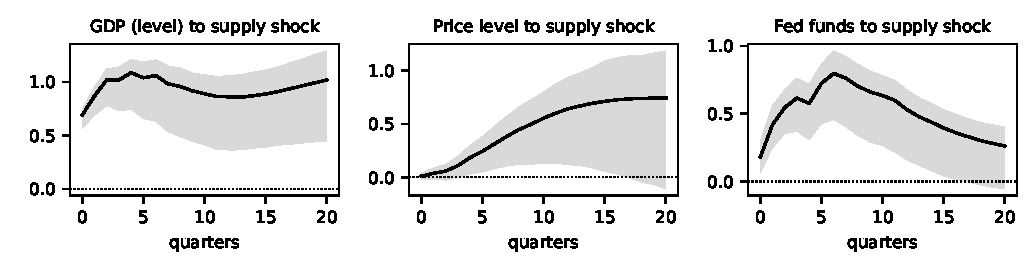
\includegraphics[width=\textwidth]{figures/ch15_14.pdf}
\end{center}

\emph{Comments.}  The shock raises output persistently --- about $1\%$ after a year and still $1\%$ after five
years (90\% band at $h=20$: $[0.44,1.29]$) --- consistent with a permanent supply improvement.  The fed funds
rate rises by up to $0.7$ points and returns toward zero, a systematic policy tightening.  But the price
level \emph{rises} steadily ($0.45\%$ at two years, band $[0.12,0.66]$), whereas a favourable aggregate supply
shock should lower prices.  So the identified ``supply'' shock behaves like a demand shock, which casts
doubt on the recursive identification of Section 15.23 (the assumption that output does not respond
to demand within the quarter).
\end{ex}

%%---------------------------------------------------------------------------
\begin{ex}{15.15}
Monthly 1973m2--2007m12, $n=415$; responses to one-standard-deviation shocks, 24 months.

\begin{center}
\begin{tabular}{lccccccc}
\toprule
months & 0 & 1 & 3 & 6 & 12 & 18 & 24\\
\midrule
oil supply shock          & $-0.32$ & $-0.42$ & $-1.47$ & $-0.71$ & $-0.71$ & $-0.61$ & $-0.53$\\
aggregate demand shock    & $4.44$ & $5.64$ & $5.40$ & $4.81$ & $4.05$ & $3.34$ & $2.71$\\
oil-specific demand shock & $0.00$ & $0.52$ & $1.17$ & $1.28$ & $0.73$ & $0.40$ & $0.14$\\
\bottomrule
\end{tabular}
\end{center}

\begin{center}
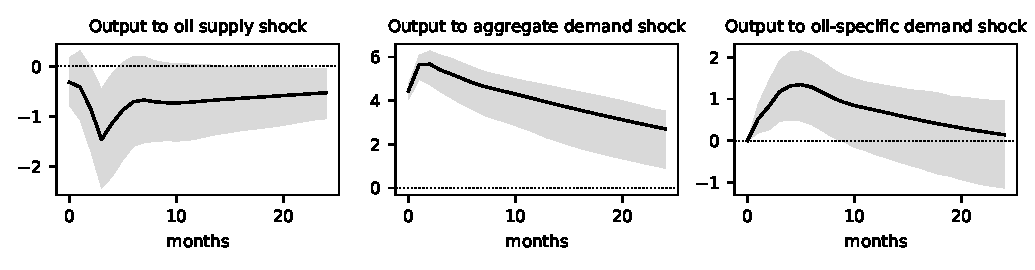
\includegraphics[width=\textwidth]{figures/ch15_15.pdf}
\end{center}

\emph{Comments.}  A supply disruption (lower oil production) lowers global real activity, with a trough of
about $-1.5$ after three months and a persistent negative effect, marginally significant at longer
horizons (90\% band at 24 months $[-1.05,-0.05]$).  An aggregate demand shock raises activity strongly and
very persistently (band at 24 months $[0.89,3.53]$) --- by construction it is the innovation in the activity
index itself.  An oil-specific (precautionary) demand shock has no impact effect by the ordering, a
small positive effect peaking at six months (band $[0.39,2.06]$), and nothing afterwards.  The main
lesson matches Kilian: global activity is driven mostly by its own demand shocks, while oil supply
shocks have modest and delayed real effects.  (For completeness, the real oil price rises by $6.1$ on impact
after an oil-specific demand shock, by $0.4$ after an aggregate demand shock rising to $4.8$ after two
years, and only briefly after a supply shock --- the pattern of Figure 15.2.)
\end{ex}

%%---------------------------------------------------------------------------
\begin{ex}{15.16}
\textbf{(a)}  Loan growth $=100\Delta\log(\text{realln})$.  Permits start in 1960m1, which fixes the sample; with eight
initial conditions $n=688$ (1960m9--2017m12).  Permits and starts are in thousands of units at annual rates.

\textbf{(b)}  $\text{AIC}=n\log|\wh\Sigma|+2\times$(number of coefficients), on the common sample:
\begin{center}
\small
\begin{tabular}{lcccccccc}
\toprule
$p$ & 1 & 2 & 3 & 4 & 5 & 6 & 7 & 8\\
\midrule
AIC & $11015.9$ & $10876.1$ & $10833.6$ & $10779.1$ & $10767.4$ & $\mathbf{10739.8}$ & $10744.8$ & $10758.2$\\
\bottomrule
\end{tabular}
\end{center}
AIC selects $p=6$.

\textbf{(c)}  Responses of housing starts (thousands, annual rate) to one-standard-deviation orthogonalized
shocks:
\begin{center}
\begin{tabular}{lccccccc}
\toprule
months & 0 & 1 & 3 & 6 & 12 & 24 & 36\\
\midrule
permit shock   & $53.5$ & $62.3$ & $71.7$ & $69.4$ & $67.5$ & $48.5$ & $32.3$\\
starts shock   & $75.7$ & $15.4$ & $18.8$ & $27.4$ & $21.3$ & $15.7$ & $11.2$\\
loan shock     & $0.0$ & $-3.9$ & $-9.1$ & $-9.8$ & $-15.7$ & $-14.3$ & $-9.9$\\
\bottomrule
\end{tabular}
\end{center}
\begin{center}
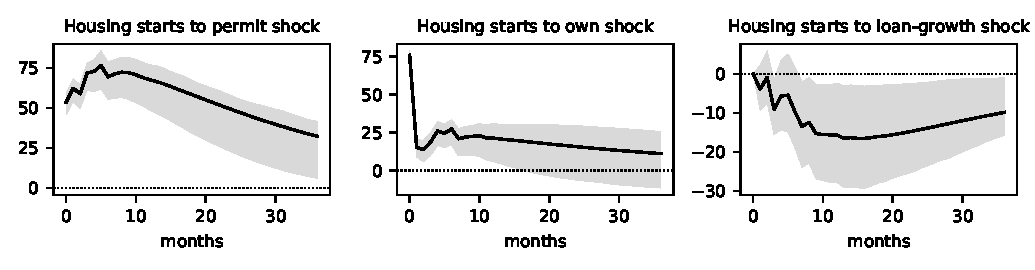
\includegraphics[width=\textwidth]{figures/ch15_16.pdf}
\end{center}

\textbf{(d)}  A permit shock raises starts immediately (because the permit and start innovations are highly
correlated, $0.58$, and permits are ordered first) and the effect builds for three months and lasts for
years: permits are the leading, persistent signal of construction.  A shock to starts that is
\emph{not} predicted by permits is mostly transitory --- it falls from $76$ to $15$ within a month --- consistent with
timing noise (weather, reporting) in monthly starts.  A shock raising real estate loan growth is
followed by \emph{lower} starts, significantly so at longer horizons (band at 24 months $[-24,-2]$).  One
reading is that loan growth reflects purchases of the existing stock and tighter subsequent credit
conditions; but this is a predictive pattern under a recursive ordering, not a structural credit-supply
effect.
\end{ex}

%%---------------------------------------------------------------------------
\begin{ex}{15.17}
Ordering $(e_I,e_P,e_Y,e_R)$ for investment, prices, GDP and the fed funds rate.

\textbf{(a)}
\[
  A=\begin{bmatrix}1&0&-1&0\\ 0&1&a_{23}&0\\ a_{31}&a_{32}&1&0\\ a_{41}&a_{42}&a_{43}&1\end{bmatrix},\qquad
  \var(\varepsilon_t)=\diag(\sigma_I^{2},\sigma_P^{2},\sigma_Y^{2},\sigma_R^{2}).
\]

\textbf{(b)}  Order condition: $6$ free coefficients plus $4$ variances $=10=m(m+1)/2$; exactly identified.  Rank
condition, equation by equation (Section 15.26): equation 1 has no free coefficient, so $\varepsilon_I=e_I-e_Y$ is
identified.  Equation 2 needs an instrument for $e_Y$ uncorrelated with $\varepsilon_P$; $\varepsilon_I$ qualifies if
$\cov(e_Y,\varepsilon_I)\neq0$.  Solving the first three equations, $\cov(e_Y,\varepsilon_I)\propto-a_{31}\sigma_I^{2}/\det(A_{11})$, so relevance
requires $a_{31}\neq0$.  Equation 3 uses $(\varepsilon_I,\varepsilon_P)$ as instruments for $(e_I,e_P)$, relevant because the
corresponding $2\times2$ block of $A_{11}^{-1}$ has determinant $1/\det A_{11}\neq0$.  Equation 4 uses all three earlier
shocks.  So the model is identified provided $a_{31}\neq0$ (GDP responds contemporaneously to investment)
and $\det A_{11}=1+a_{31}-a_{23}a_{32}\neq0$.

\textbf{(c)}  Simultaneous: the price equation contains $e_Y$ and the GDP equation contains $e_P$.  Unlike the
recursive example of Section 15.23, neither is predetermined within the quarter.

\textbf{(d)}  AIC (VARs with trend, $p=1,\dots,8$) is minimized at $p=6$, which justifies six lags.  Solving
$A\wh\Sigma A'=$ diagonal (the solution is unique):
\[
  \wh A=\begin{bmatrix}1&0&-1&0\\0&1&-0.062&0\\-0.154&0.403&1&0\\-0.043&-0.590&-0.096&1\end{bmatrix},
  \qquad \wh\sigma_\varepsilon=(2.63,\ 0.22,\ 0.41,\ 0.65).
\]
Written as structural equations: $e_P=0.062e_Y+\varepsilon_P$ (prices rise slightly with output, Phillips-curve
like); $e_Y=0.154e_I-0.403e_P+\varepsilon_Y$ (output rises with investment and falls with prices, a demand
relation); $e_R=0.043e_I+0.590e_P+0.096e_Y+\varepsilon_R$ (a Taylor-type rule responding mainly to prices).  The
signs are economically sensible.

\textbf{(e)}  Variables are in log levels, so responses need no cumulation (units: $\%$ for GDP and prices).
\begin{center}
\begin{tabular}{lccccccc}
\toprule
quarters & 0 & 1 & 2 & 4 & 8 & 12 & 20\\
\midrule
GDP to fed funds shock & $0.00$ & $0.03$ & $-0.18$ & $-0.32$ & $-0.59$ & $-0.53$ & $-0.32$\\
GDP to GDP shock       & $0.47$ & $0.56$ & $0.65$ & $0.62$ & $0.23$ & $0.07$ & $0.13$\\
prices to GDP shock    & $0.03$ & $0.06$ & $0.10$ & $0.21$ & $0.44$ & $0.59$ & $0.62$\\
\bottomrule
\end{tabular}
\end{center}
\begin{center}
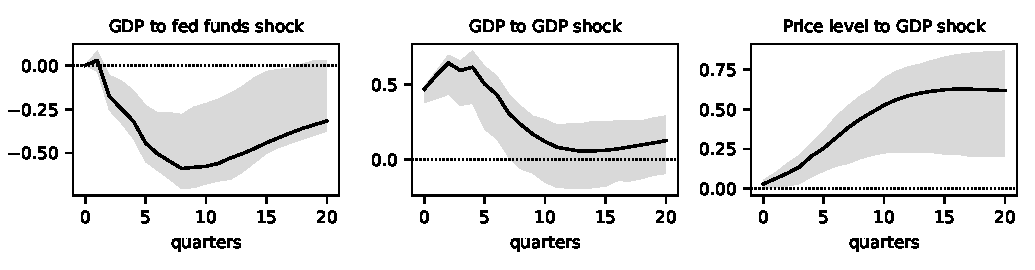
\includegraphics[width=\textwidth]{figures/ch15_17.pdf}
\end{center}
A monetary tightening ($0.65$ points) lowers GDP with a lag, by about $0.6\%$ after two years (band at 12 quarters
$[-0.65,-0.16]$) --- the textbook contractionary effect.  The GDP shock raises output temporarily (back near
zero after three years) while the price level rises steadily ($0.59\%$ at 12 quarters, band $[0.23,0.77]$): the
GDP shock behaves like an aggregate demand shock.
\end{ex}

%%---------------------------------------------------------------------------
\begin{ex}{15.18}
Ordering (supply $=-$oil, output, price).

\textbf{(a)}  $A=\begin{bmatrix}1&0&0\\0&1&a_{23}\\a_{31}&a_{32}&1\end{bmatrix}$ with diagonal shock covariance.

\textbf{(b)}  Order condition: $3+3=6=m(m+1)/2$, exactly identified.  Equation 1 has no free coefficients.
Equation 2 (output) needs $\varepsilon_1$ as instrument for the price innovation; relevance requires
$\cov(e_{3},\varepsilon_1)\propto-a_{31}\neq0$ --- the oil price must respond contemporaneously to supply shocks.  Equation 3
uses $(\varepsilon_1,\varepsilon_2)$, which is relevant whenever $1-a_{23}a_{32}\neq0$.  So identification requires $a_{31}\neq0$.

\textbf{(c)}  Four lags, as in Exercise 15.15 and Section 15.24, for comparability (monthly data would
support more).  The unique solution is
\[
  \wh A=\begin{bmatrix}1&0&0\\0&1&1.530\\-0.053&-2.622&1\end{bmatrix},\qquad \wh\sigma_\varepsilon=(20.0,\ 10.6,\ 12.8),
\]
i.e.\ $e_{\text{output}}=-1.53e_{\text{price}}+\varepsilon_2$ and $e_{\text{price}}=0.053e_{\text{supply}}+2.62e_{\text{output}}+\varepsilon_3$.  The implied
simultaneous effects are large, but they should not be taken at face value: the estimate
$\wh a_{31}=-0.053$ is close to zero and the correlation between the supply and price innovations is only
$0.03$.  The identifying condition $a_{31}\neq0$ is nearly violated, so the output equation is \emph{weakly}
identified --- the structural VAR analogue of a weak instrument.

\textbf{(d)}  Responses of the real oil price to one-standard-deviation structural shocks:
\begin{center}
\begin{tabular}{lccccccc}
\toprule
months & 0 & 1 & 3 & 6 & 12 & 18 & 24\\
\midrule
supply shock           & $0.21$ & $0.21$ & $1.32$ & $0.98$ & $0.48$ & $0.14$ & $-0.11$\\
aggregate demand shock & $5.54$ & $8.12$ & $8.11$ & $7.58$ & $7.48$ & $7.07$ & $6.51$\\
oil-specific demand    & $2.55$ & $3.32$ & $2.94$ & $1.74$ & $0.09$ & $-1.09$ & $-1.88$\\
\bottomrule
\end{tabular}
\end{center}
\begin{center}
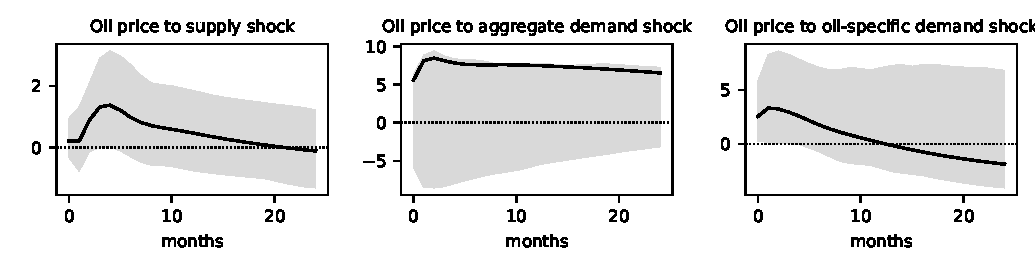
\includegraphics[width=\textwidth]{figures/ch15_18.pdf}
\end{center}
Compared with the recursive VAR of Exercise 15.15 (impact responses $0.21$, $0.40$, $6.09$), this model attributes
most of the contemporaneous oil-price variation to aggregate demand rather than to oil-specific demand,
and makes the demand effect large and persistent.  But the bootstrap bands are extremely wide (at six
months the 90\% band for the aggregate-demand response is $[-7.3,8.2]$), reflecting the weak identification
in (c).  The data cannot distinguish these structural stories; the recursive model's zero restriction on
the response of activity to prices is doing a great deal of work in Kilian's results.
\end{ex}

%%---------------------------------------------------------------------------
\begin{ex}{15.19}
Growth rates are $100\Delta\log$; $n=231$.

\textbf{(a)}  Money growth coefficients (lags 1--4): $0.044\ (0.057)$, $0.094\ (0.066)$, $-0.147\ (0.054)$, $0.048\ (0.051)$.
Wald statistic $8.98$, $\chi^{2}_4$ $p=0.062$.  Strict neutrality is not rejected at $5\%$ (it would be at $10\%$): there is
at most weak evidence that money growth helps predict GDP growth.

\textbf{(b)}  Sum of the money coefficients $0.038\ (0.039)$, $t=0.97$, $p=0.33$.  Long-run neutrality is not
rejected; the individual coefficients largely offset.

\textbf{(c)}  Estimate a VAR(4) in $(\Delta\text{GDP},\Delta\text{M1})$.  Let $A(1)=\I-\wh A_1-\cdots-\wh A_4$ and define the long-run response
matrix $C=A(1)^{-1}B$.  Long-run neutrality says the second (nominal) shock has no long-run effect on the level
of GDP: $C_{12}=0$, so $C$ is lower triangular and, as in Blanchard--Quah,
$\wh C=\operatorname{chol}\bigl(\wh A(1)^{-1}\wh\Sigma\wh A(1)^{-1\prime}\bigr)$, $\wh B=\wh A(1)\wh C$.  Estimates:
$\wh C=\begin{bmatrix}1.367&0\\-0.791&3.212\end{bmatrix}$, $\wh B=\begin{bmatrix}0.739&-0.123\\0.081&0.942\end{bmatrix}$.  The first shock is the
``real'' shock (the only one with permanent output effects), the second the ``nominal'' shock.

\textbf{(d)}  Cumulated responses (levels, \%):
\begin{center}
\begin{tabular}{lccccccc}
\toprule
quarters & 0 & 1 & 2 & 4 & 8 & 12 & 24\\
\midrule
GDP to real shock      & $0.74$ & $0.94$ & $1.17$ & $1.29$ & $1.37$ & $1.37$ & $1.37$\\
GDP to nominal shock   & $-0.12$ & $-0.12$ & $-0.03$ & $-0.05$ & $-0.03$ & $-0.01$ & $0.00$\\
M1 to real shock       & $0.08$ & $0.01$ & $-0.09$ & $-0.31$ & $-0.59$ & $-0.72$ & $-0.79$\\
M1 to nominal shock    & $0.94$ & $1.44$ & $1.81$ & $2.36$ & $2.90$ & $3.10$ & $3.21$\\
\bottomrule
\end{tabular}
\end{center}
\begin{center}
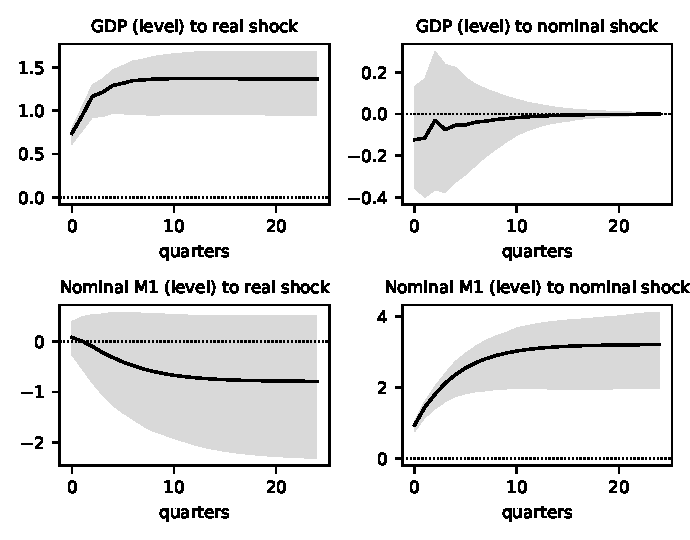
\includegraphics[width=0.8\textwidth]{figures/ch15_19.pdf}
\end{center}
The real shock raises GDP permanently by about $1.4\%$ and (insignificantly) lowers nominal money.  The
nominal shock permanently raises money by $3.2\%$ but has only a tiny, short-lived and \emph{negative} effect on
output (band at four quarters $[-0.33,0.22]$).  There is no evidence here of short-run non-neutrality
either, consistent with (a).  Of course the long-run neutrality result is imposed, not estimated: the
exercise shows what the data look like \emph{given} that identifying assumption.
\end{ex}

%%---------------------------------------------------------------------------
\begin{ex}{15.20}
\textbf{(a)}  With ordering (hours, GDP, inflation) and shocks (labor supply, technology, demand),
\[
  C=\begin{bmatrix}c_{11}&0&0\\c_{21}&c_{22}&0\\c_{31}&c_{32}&c_{33}\end{bmatrix}.
\]

\textbf{(b)}  Yes, exactly: identification needs $m(m-1)/2=3$ restrictions and three zeros are imposed.  Because
$C$ is lower triangular, $CC'=A(1)^{-1}\Sigma A(1)^{-1\prime}$ has the unique Cholesky solution (with positive diagonal).

\textbf{(c)}  On a common sample ($n=225$), AIC for $p=1,\dots,8$:
$-1075.0$, $-1086.2$, $-1083.6$, $\mathbf{-1086.6}$, $-1075.8$, $-1067.0$, $-1058.8$, $-1070.5$.  AIC selects $p=4$.

\textbf{(d)}
\[
  \wh C=\begin{bmatrix}1.530&0&0\\1.060&0.700&0\\0.045&0.023&0.146\end{bmatrix}.
\]
Entries are long-run effects of one-standard-deviation shocks on the levels of hours and GDP ($\%$) and on
the \emph{level} of inflation (the cumulated change).  A labor-supply shock raises hours by $1.53\%$ and GDP by
$1.06\%$ in the long run --- an implied output elasticity of $0.69$, close to labor's income share.  A technology
shock raises GDP by $0.70\%$ with no long-run effect on hours.  Demand shocks move only long-run inflation
($0.15$ points).

\textbf{(e)}  Level of GDP (\%):
\begin{center}
\begin{tabular}{lccccccc}
\toprule
quarters & 0 & 1 & 2 & 4 & 8 & 12 & 24\\
\midrule
labor-supply shock & $0.61$ & $0.85$ & $1.05$ & $1.15$ & $1.10$ & $1.06$ & $1.06$\\
technology shock   & $0.37$ & $0.36$ & $0.46$ & $0.66$ & $0.71$ & $0.70$ & $0.70$\\
demand shock       & $0.13$ & $0.13$ & $0.11$ & $0.01$ & $-0.01$ & $0.00$ & $0.00$\\
\bottomrule
\end{tabular}
\end{center}
\begin{center}
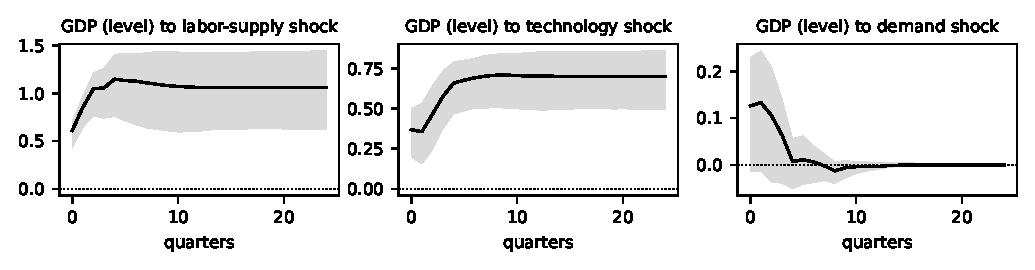
\includegraphics[width=\textwidth]{figures/ch15_20.pdf}
\end{center}
Both supply shocks have permanent, precisely estimated effects that are mostly in place within a year;
labor-supply shocks are the larger source of long-run output movements.  Demand shocks raise output
briefly ($0.13\%$) and die out within a year, and their effect is statistically indistinguishable from zero at
every horizon beyond impact.  The results mirror Shapiro and Watson's conclusion that permanent output
movements are driven by supply-side shocks.
\end{ex}

%% ===========================================================================
%% Chapter 16. Non-Stationary Time Series
%% ===========================================================================
\solchapter{16}{Non-Stationary Time Series}

\begin{center}
\begin{minipage}{0.86\textwidth}
\small
Solutions to all 14 exercises of Chapter 16 of Bruce E.\ Hansen, \emph{Econometrics}
(Princeton University Press, 2022).  Exercises 16.12--16.14 use \texttt{FRED-MD} (1959m1--2017m12, $708$
months).  P-values are asymptotic, interpolated linearly from the book's Tables 16.1 and 16.6--16.8 as
described in Section 16.13.  The code was checked against the book: it reproduces Table 16.2 (ADF and
KPSS), the Engle--Granger statistic $-4.0$, the VECM estimates of Tables 16.4--16.5 and the trace statistics
$31.6$, $2.8$ and Table 16.9 ($120$, $68.3$, $33.6$, $10.8$).
\end{minipage}
\end{center}

\bigskip
\hrule
\bigskip

Notation: $W(r)$ is standard Brownian motion; $\Rightarrow$ and $\convd$ both denote convergence in distribution, the
former for processes on $[0,1]$.  ``Case 1/2/3'' refer to ADF regressions with no deterministic terms, an
intercept, and an intercept and linear trend (the three ADF columns of Table 16.1).

%%---------------------------------------------------------------------------
\begin{ex}{16.1}
\textbf{(a)}  $S_t=\sum_{i=1}^{t}e_i$, so $\E[S_t]=0$ and $\var[S_t]=t\sigma^{2}$.

\textbf{(b)}  $Y_t=S_t/(\sigma\sqrt t)$.  Mean and variance are constant, but for $k\ge0$
\[
  \cov(Y_t,Y_{t+k})=\frac{\cov(S_t,S_t+e_{t+1}+\cdots+e_{t+k})}{\sigma^{2}\sqrt{t(t+k)}}=\frac{t\sigma^{2}}{\sigma^{2}\sqrt{t(t+k)}}=\sqrt{\frac{t}{t+k}},
\]
which depends on $t$ (e.g.\ $\cov(Y_1,Y_2)=0.71$ but $\cov(Y_{100},Y_{101})=0.995$).  So $Y_t$ is \textbf{not} covariance
stationary, and hence not strictly stationary either.  (With non-normal errors even the marginal
distribution changes with $t$: $Y_1=e_1/\sigma$ while $Y_t$ is approximately normal for large $t$.)  Standardizing
the first two moments does not remove the non-stationarity, which lives in the dependence structure.

\textbf{(c)}  By Theorem 16.1, $n^{-1/2}S_{\lfloor nr\rfloor}\Rightarrow\sigma W(r)$ on $[0,1]$, and $\lfloor nr\rfloor/n\to r$ uniformly in $r$.  Since
\[
  Y_{\lfloor nr\rfloor}=\frac{n^{-1/2}S_{\lfloor nr\rfloor}}{\sigma\sqrt{\lfloor nr\rfloor/n}}
\]
and $(f,g)\mapsto f/\sqrt g$ is continuous on functions with $g\ge\delta/2>0$, the continuous mapping theorem gives
\[
  Y_{\lfloor nr\rfloor}\Rightarrow \frac{W(r)}{\sqrt r},\qquad r\in[\delta,1].
\]
For each fixed $r$ the limit is $N(0,1)$, but as a process it is not stationary:
$\cov\bigl(W(r)/\sqrt r,\,W(s)/\sqrt s\bigr)=\sqrt{r/s}$ for $r\le s$.  The restriction $r\ge\delta>0$ is needed because the scaling
$1/\sqrt r$ explodes at $r=0$.
\end{ex}

%%---------------------------------------------------------------------------
\begin{ex}{16.2}
Write $\Theta(z)=\Theta(1)+(1-z)\Theta^{*}(z)$ with $\Theta(1)=\I+\Theta_1+\Theta_2$ and, by (16.4), $\Theta_j^{*}=-\sum_{\ell>j}\Theta_\ell$:
\[
  \Theta_0^{*}=-(\Theta_1+\Theta_2),\qquad \Theta_1^{*}=-\Theta_2,\qquad \Theta_j^{*}=\bzero\ (j\ge2).
\]
Check: $\Theta(1)+(1-z)(\Theta_0^{*}+\Theta_1^{*}z)=\Theta(1)+\Theta_0^{*}+(\Theta_1^{*}-\Theta_0^{*})z-\Theta_1^{*}z^{2}=\I+\Theta_1z+\Theta_2z^{2}$.  Hence
\[
  \Delta Y_t=\xi_t+U_t-U_{t-1},\qquad \xi_t=(\I+\Theta_1+\Theta_2)e_t,\qquad U_t=-(\Theta_1+\Theta_2)e_t-\Theta_2e_{t-1},
\]
and summing, $Y_t=S_t+U_t+V_0$ with permanent component $S_t=(\I+\Theta_1+\Theta_2)\sum_{i=1}^{t}e_i$, transitory MA(1)
component $U_t$, and initial condition $V_0=Y_0-U_0$.  For $\Theta_2=\bzero$ this reduces to the book's MA(1) example.
\end{ex}

%%---------------------------------------------------------------------------
\begin{ex}{16.3}
Assume, as in Theorem 16.4, that $(e_t,u_t)$ is strictly stationary with finite variances and summable
autocovariances, $X_0$ finite, and let $\omega_e^{2}>0$ be the long-run variance of $e_t$.

\textbf{(a)}  $\Delta Y_t=e_t+u_t-u_{t-1}$ is stationary.  Its long-run variance is the value at frequency zero of the
spectral density.  The filter $1-L$ vanishes at frequency zero, so $\Delta u_t$ contributes nothing, neither on its
own nor through its cross-covariance with $e_t$:
\[
  \omega^{2}_{\Delta Y}=\sum_{\ell=-\infty}^{\infty}\cov(\Delta Y_t,\Delta Y_{t-\ell})=\omega_e^{2}>0 .
\]
Hence $\Delta Y_t$ is $I(0)$ and $Y_t$ is $I(1)$.  (Directly: $Y_t$ has variance growing like $t\,\omega_e^{2}$, so it is not stationary.)

\textbf{(b)}  $n^{-1/2}Y_{\lfloor nr\rfloor}=n^{-1/2}X_0+n^{-1/2}\sum_{t\le\lfloor nr\rfloor}e_t+n^{-1/2}u_{\lfloor nr\rfloor}$.  The first term is $o_p(1)$.  The
second converges to $\omega_eW(r)$ by the FCLT (Theorem 16.4).  For the third, by the union bound and
strict stationarity,
\[
  \Pb{\max_{t\le n}|u_t|>\varepsilon\sqrt n}\le n\,\Pb{|u_1|>\varepsilon\sqrt n}\le\varepsilon^{-2}\,\E\bigl[u_1^{2}\indic\{|u_1|>\varepsilon\sqrt n\}\bigr]\to0,
\]
so it is $o_p(1)$ uniformly in $r$.  Therefore $n^{-1/2}Y_{\lfloor nr\rfloor}\Rightarrow\omega_eW(r)$, a Brownian motion with variance $\omega_e^{2}$: the
stationary noise is asymptotically invisible at this scale.
\end{ex}

%%---------------------------------------------------------------------------
\begin{ex}{16.4}
Let $\sigma^{2}=\var[e_t]>0$.

\textbf{(a)}  An i.i.d.\ sequence is strictly (hence weakly, given $\sigma^{2}<\infty$) stationary.  All autocovariances beyond
lag zero vanish, so the long-run variance is $\sigma^{2}>0$, and $Y_t$ is $I(0)$ by Definition 16.2.

\textbf{(b)}  $X_t=e_t-e_{t-1}$ is an MA(1), a fixed function of the stationary pair $(e_t,e_{t-1})$, so it is stationary.
Its autocovariances are $\gamma(0)=2\sigma^{2}$, $\gamma(\pm1)=-\sigma^{2}$, and $0$ otherwise, so its long-run variance is
$\omega^{2}=2\sigma^{2}-2\sigma^{2}=0$ (equivalently $b(1)^{2}\sigma^{2}$ with $b(z)=1-z$).  Definition 16.2 requires a positive long-run variance,
so $X_t$ is not $I(0)$.  It is over-differenced ($I(-1)$): its partial sums $\sum_{t\le n}X_t=e_n-e_0$ stay bounded in probability
instead of growing like $\sqrt n$.
\end{ex}

%%---------------------------------------------------------------------------
\begin{ex}{16.5}
Both series load on the random walk $U_t$, so both are $I(1)$ (assuming $\var[e_t]>0$).  The combination
$\beta'(Y_t,X_t)'=\beta_1Y_t+\beta_2X_t=(\beta_1+2\beta_2)U_t+\beta_1v_t+\beta_2w_t$ is stationary if and only if $\beta_1+2\beta_2=0$.  So the cointegrating
vector is
\[
  \beta=(2,\,-1)'\quad\text{or, normalized},\quad \beta=(1,\,-\tfrac12)',
\]
with equilibrium error $2Y_t-X_t=2v_t-w_t$, i.i.d.\ and hence $I(0)$ provided $\var[2v_t-w_t]>0$.  It is unique up to
scale, since any other direction leaves $U_t$ in the combination.
\end{ex}

%%---------------------------------------------------------------------------
\begin{ex}{16.6}
\emph{The limits are consistent at the boundary.}  As $\alpha\to1$ the stationary variance $1-\alpha^{2}\to0$: the $\sqrt n$-normalized
estimator becomes degenerate, which signals that a faster rate applies.  At $\alpha=1$ indeed
$\sqrt n(\wh\alpha-1)=n^{-1/2}\cdot n(\wh\alpha-1)=O_p(n^{-1/2})\convp0$, matching the ``$N(0,0)$'' limit.  With the correct rate $n$, Theorem 16.9
gives the non-degenerate Dickey--Fuller distribution $\int_0^1W\,dW/\int_0^1W^{2}$, which is skewed to the left (median below
zero), so $\wh\alpha$ is biased downward.

\emph{The convergence is not uniform.}  For each fixed $|\alpha|<1$ the normal approximation eventually works, but
the sample size needed grows without bound as $\alpha\to1$.  What matters is $n(1-\alpha)$, the number of
``half-lives'' in the sample.  The unifying device is local-to-unity asymptotics, $\alpha_n=1+c/n$ with $c\le0$ fixed,
under which
\[
  n(\wh\alpha-\alpha_n)\convd\frac{\int_0^1J_c\,dW}{\int_0^1J_c^{2}},\qquad J_c(r)=\int_0^re^{c(r-s)}dW(s),
\]
an Ornstein--Uhlenbeck process.  This family equals the Dickey--Fuller distribution at $c=0$ and, suitably
rescaled, tends to the normal as $c\to-\infty$.  In practice, when $n(1-\wh\alpha)$ is not large (say $\wh\alpha=0.95$ with
$n=100$) the $N(0,1-\alpha^{2})$ approximation is poor: $t$-ratios are skewed and conventional confidence intervals
under-cover.  Unit-root distributions, or intervals obtained by inverting such tests (Stock 1991;
Hansen's 1999 grid bootstrap), should be used.
\end{ex}

%%---------------------------------------------------------------------------
\begin{ex}{16.7}
Premultiply by $\beta'$: $\beta'Y_t-\beta'Y_{t-1}=\beta'\alpha\,\beta'Y_{t-1}+\beta'e_t$, i.e.
\[
  Z_t=(\I_r+\beta'\alpha)Z_{t-1}+\beta'e_t,
\]
an AR(1) (a VAR(1) when $r>1$) with coefficient $\I_r+\beta'\alpha$ and white-noise error $\beta'e_t$.  $Z_t$ is stationary if all
eigenvalues of $\I_r+\beta'\alpha$ lie inside the unit circle.  In the scalar case this means $-2<\beta'\alpha<0$: the adjustment
coefficients must push the equilibrium error back toward zero without overshooting.
\end{ex}

%%---------------------------------------------------------------------------
\begin{ex}{16.8}
Yes.  The statistic is $t=(0.9-1)/0.05=-2$, and they are implicitly comparing it with a normal critical value
($|t|>1.96$).  Under $H_0:\alpha=1$ the $t$-ratio does not have an asymptotic normal distribution but the
Dickey--Fuller $t$ distribution (Theorem 16.10), and the test is one-sided (reject for large negative values).
The right critical value depends on the deterministic terms.
\begin{itemize}[leftmargin=*]
\item As literally written (no intercept, Case 1): the 5\% critical value is $-1.94$ and the interpolated p-value
is $0.04+0.01\times(2.03-2.00)/0.09\approx0.043$.  The test barely rejects at 5\%, but for the wrong reason.
\item With an intercept, which is the usual specification since a no-intercept regression is appropriate only for
data with a known zero mean (Case 2): the 5\% critical value is $-2.86$ and the p-value is
$0.20+0.10\times(2.22-2.00)/0.25\approx0.29$.  No rejection.
\end{itemize}
Further caveats: the regression should include enough lagged differences for $e_t$ to be serially
uncorrelated (the ADF test), and failing to reject would not establish a unit root.
\end{ex}

%%---------------------------------------------------------------------------
\begin{ex}{16.9}
Yes.  The arithmetic is right ($0.9\pm1.96\times0.04$), but the interval is justified by normal asymptotics, which
fail near and at $\alpha=1$ (Exercise 16.6).  Whether $\alpha=1$ is consistent with the data must be judged by the
unit root distribution of $t=(0.9-1)/0.04=-2.5$:
\begin{itemize}[leftmargin=*]
\item no intercept (Case 1): p-value $\approx0.01+0.01\times(2.56-2.50)/0.25=0.012$, a rejection at 5\%;
\item intercept (Case 2): p-value $\approx0.10+0.05\times(2.57-2.50)/0.20=0.12$, no rejection;
\item intercept and trend (Case 3): p-value $\approx0.33$, no rejection.
\end{itemize}
In the realistic specifications $\alpha=1$ is \emph{not} rejected, so it belongs in any valid 95\% confidence set.  The
normal interval has the wrong coverage, because the $t$-ratio is skewed and the correct interval is not
symmetric about $\wh\alpha$.  A valid set collects the values $\alpha_0$ not rejected by a test with the right
(local-to-unity) critical values, or comes from a grid bootstrap.  And even a rejection only says that
$\alpha=1$ is unlikely, not that it is ``inconsistent with the data''.
\end{ex}

%%---------------------------------------------------------------------------
\begin{ex}{16.10}
Yes.  The critical value $-1.9$ is the Case 1 value ($-1.94$ in Table 16.1): the software treats $Z_t$ as a series
with no estimated deterministic components.  But the trend was estimated in the first step, and
detrending by least squares beforehand is algebraically equivalent (asymptotically) to including the
trend in the ADF regression.  The statistic therefore follows the \emph{detrended} Dickey--Fuller distribution
(Theorem 16.14, Case 3), with 5\% critical value $-3.41$.  Against the correct
table,
\[
  p\approx0.30+0.20\times\frac{2.56-2.50}{2.56-2.18}\approx0.33,
\]
so the unit root is \emph{not} rejected.  (Even under Case 1 the p-value would be about $1.2\%$, not below $1\%$.)
Estimating deterministic terms shifts the null distribution to the left; ignoring this makes stationarity
far too easy to ``find''.
\end{ex}

%%---------------------------------------------------------------------------
\begin{ex}{16.11}
Yes, several.
\begin{enumerate}[leftmargin=*]
\item \emph{Non-rejection is not acceptance.}  With an intercept the p-value is about $0.20+0.10\times0.22/0.25\approx0.29$.  The test
fails to reject a unit root, which means only that the data do not provide strong evidence against it.
Unit root tests have low power against persistent stationary alternatives, especially in short samples.
The correct statement is ``we cannot reject the hypothesis of a unit root.''
\item \emph{A unit root is implausible for this variable.}  A daily tweet count is non-negative and bounded in practice.  A
unit root process has variance growing linearly in time and eventually wanders arbitrarily far in both
directions, which a count cannot do.  Theory and context favour a stationary (possibly highly
persistent) count process.
\item \emph{Other features can masquerade as a unit root.}  Level shifts (a new office, a campaign, a platform change),
day-of-week effects and heteroskedasticity typical of count data all reduce the power of the ADF test
(Perron 1989).  A count model (e.g.\ Poisson autoregression) with breaks would be more appropriate.
\end{enumerate}
Consistent with Section 16.13, the test should be used to check a modeling presumption, not as a
rule for declaring a series a unit root process.
\end{ex}

%%---------------------------------------------------------------------------
\begin{ex}{16.12}
\emph{Method.}  The trend specification is chosen from the nature of the series (plotted below): a linear
trend (Case 3) for the growing aggregates in (a), (b), (e), (g) and for \emph{hwi}, which in this vintage (spliced
with JOLTS data) trends upward; an intercept only (Case 2) for housing starts and initial claims, which
fluctuate around a stable level.  Aggregates growing exponentially are logged (the book lists \emph{indpro},
\emph{clf16ov} and \emph{ipfuels} in levels; their level results are given in the notes).  The order $p$ minimizes AIC over
AR($p$), $p\le12$, fit with the same deterministic terms on a common sample starting 1960m1.  The ADF
regression $\Delta Y_t=\mu(+\delta t)+\rho Y_{t-1}+\sum_{j=1}^{p-1}\gamma_j\Delta Y_{t-j}+e_t$ then uses all available observations.  (Book typo: the
FRED-MD mnemonic for initial claims is \emph{claimsx}, not \emph{claims}.)

\begin{center}
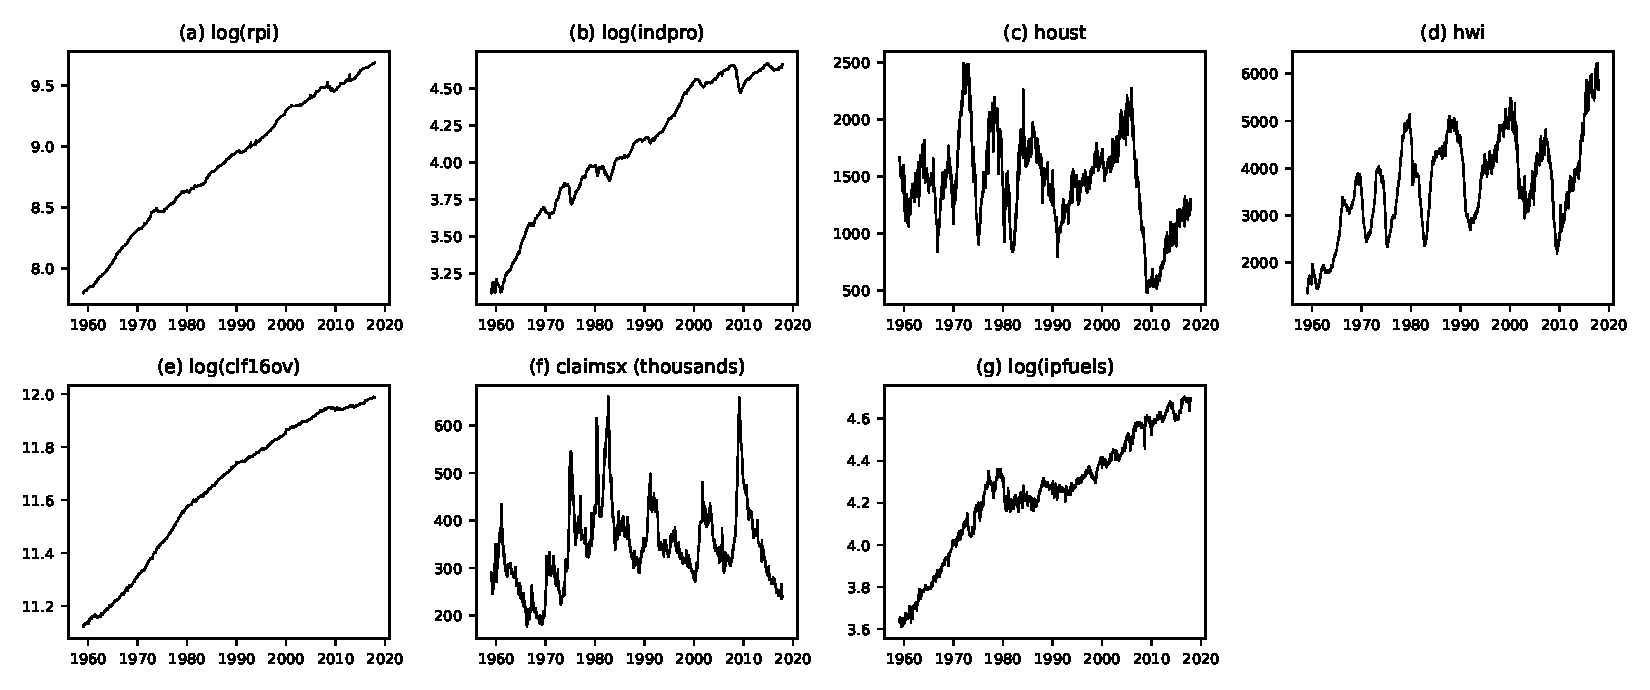
\includegraphics[width=\textwidth]{figures/ch16_12.pdf}
\end{center}

\begin{center}
\small
\begin{tabular}{llcccc}
\toprule
series & deterministic & $p$ & $\wh\rho$ (s.e.) & ADF & p-value\\
\midrule
(a) $\log(\textit{rpi})$     & trend     & 9  & $-0.0075$ $(0.0036)$ & $-2.09$ & $0.55$\\
(b) $\log(\textit{indpro})$  & trend     & 6  & $-0.0051$ $(0.0029)$ & $-1.74$ & $0.73$\\
(c) \emph{houst}             & intercept & 8  & $-0.0339$ $(0.0105)$ & $-3.22$ & $0.019$\\
(d) \emph{hwi}               & trend     & 10 & $-0.0271$ $(0.0070)$ & $-3.88$ & $0.013$\\
(e) $\log(\textit{clf16ov})$ & trend     & 8  & $\phantom{-}0.0023$ $(0.0018)$ & $\phantom{-}1.27$ & $>0.99$\\
(f) \emph{claimsx}           & intercept & 7  & $-0.0313$ $(0.0084)$ & $-3.72$ & $0.006$\\
(g) $\log(\textit{ipfuels})$ & trend     & 6  & $-0.0201$ $(0.0085)$ & $-2.36$ & $0.41$\\
\bottomrule
\end{tabular}
\end{center}

\emph{Notes on alternatives.}  In levels with trend: \emph{indpro} $p=5$, ADF $=-3.02$ ($p=0.13$); \emph{clf16ov} $p=12$, ADF $=0.33$
($p>0.99$); \emph{ipfuels} $p=3$, ADF $=-2.64$ ($p=0.27$).  Adding a trend to \emph{houst} gives $-3.47$ ($0.044$), to \emph{claimsx}
$-3.71$ ($0.022$); \emph{hwi} with intercept only gives $-3.22$ ($0.019$).  The intercept-only test on $\log(\textit{clf16ov})$ gives
$-4.51$ ($p<0.001$).  This is a spurious rejection from the wrong specification: the concave growth path
makes $\Delta Y_t$ fall as $Y_{t-1}$ rises, which looks like mean reversion when no trend is allowed.

\emph{Interpretation.}
\begin{itemize}[leftmargin=*]
\item Income, industrial production, the labor force and fuel production are consistent with unit roots
(p-values $0.41$--$0.99$), as expected for macroeconomic aggregates.  For the labor force $\wh\rho>0$: growth
has decelerated since the 1990s, a shape a linear trend cannot capture.
\item Housing starts and initial claims reject the unit root at 2\% and 1\%, consistent with cyclical,
mean-reverting series, though reversion is slow: the autoregressive coefficients sum to about $0.97$.
\item \emph{hwi} rejects at about 1\%.  But the series is a splice of the print help-wanted index and online vacancy data, and its
behaviour changes markedly after 2010, so the rejection should be read cautiously (see also the KPSS results in
Exercise 16.13).
\end{itemize}
\end{ex}

%%---------------------------------------------------------------------------
\begin{ex}{16.13}
Same transformations and deterministic specifications as in Exercise 16.12: KPSS$_2$ (detrended) for
trending series, KPSS$_1$ (demeaned) otherwise.  Following Section 16.14, $M=\lfloor3n^{1/3}\rfloor=26$ ($n=708$).  This is
large enough to control size for AR(1)-type persistence up to about $0.8$.  For sensitivity we also report
$M=6\approx4(n/100)^{1/4}$, a common short-lag rule.

\begin{center}
\small
\begin{tabular}{llcccc}
\toprule
series & test & KPSS ($M=26$) & p-value & KPSS ($M=6$) & p-value\\
\midrule
(a) $\log(\textit{rpi})$     & KPSS$_2$ & $0.446$ & $<0.001$ & $1.596$ & $<0.001$\\
(b) $\log(\textit{indpro})$  & KPSS$_2$ & $0.354$ & $<0.001$ & $1.219$ & $<0.001$\\
(c) \emph{houst}             & KPSS$_1$ & $0.455$ & $0.052$  & $1.454$ & $<0.001$\\
(d) \emph{hwi}               & KPSS$_2$ & $0.176$ & $0.026$  & $0.551$ & $<0.001$\\
(e) $\log(\textit{clf16ov})$ & KPSS$_2$ & $0.649$ & $<0.001$ & $2.423$ & $<0.001$\\
(f) \emph{claimsx}           & KPSS$_1$ & $0.423$ & $0.064$  & $1.283$ & $<0.001$\\
(g) $\log(\textit{ipfuels})$ & KPSS$_2$ & $0.320$ & $0.001$  & $1.126$ & $<0.001$\\
\bottomrule
\end{tabular}
\end{center}
In levels: \emph{indpro} $0.194$ ($p=0.018$), \emph{clf16ov} $0.512$ ($<0.001$), \emph{ipfuels} $0.278$ ($0.005$).

\emph{Choice of $M$ matters.}  With $M=6$ every series rejects stationarity decisively, but a short truncation
underestimates the long-run variance of a persistent stationary series and over-rejects.  Under the
unit root alternative the statistic falls roughly like $1/M$, as the table illustrates.  We base conclusions on
$M=26$.

\emph{Combining with the ADF results.}
\begin{itemize}[leftmargin=*]
\item (a), (b), (e), (g): KPSS rejects stationarity strongly and ADF does not reject a unit root.  The two tests
agree: these aggregates are best treated as $I(1)$.
\item (c) housing starts and (f) initial claims: ADF rejects a unit root while KPSS$_1$ does not reject stationarity at
5\% ($p=0.05$ and $0.06$, borderline).  Taken together the evidence favours stationary but very persistent
series.
\item (d) \emph{hwi}: both tests reject their nulls (ADF $p=0.013$, KPSS$_2$ $p=0.026$).  Neither ``trend stationary'' nor
``unit root'' describes the series well.  The conflict is typical of a series with structural breaks
(here the shift from print to online job advertising and the associated splice), and a
break-robust analysis would be needed.
\end{itemize}
\end{ex}

%%---------------------------------------------------------------------------
\begin{ex}{16.14}
The VAR order minimizes AIC over levels VARs with $p\le12$ (common sample from 1960m1).  The trace statistic is
$\text{LR}(r)=-n\sum_{j>r}\log(1-\wh\lambda_j)$, compared with Tables 16.6--16.8 using $m-r$ degrees of freedom.

\begin{center}
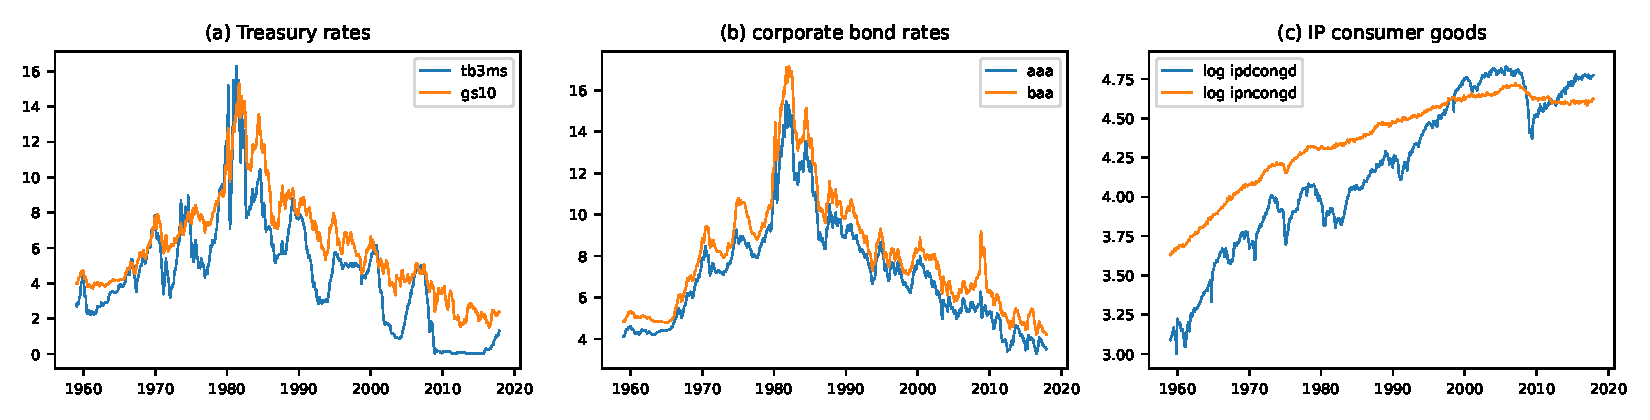
\includegraphics[width=\textwidth]{figures/ch16_14.pdf}
\end{center}

\emph{Trend specification.}  Interest rates are untrended, so we use Trend Model 2 (intercept restricted to the
cointegrating relation).  The IP series are trended and grow at different average rates
($2.9\%$ versus $1.7\%$ a year), so any cointegrating relation must allow a linear trend.  We report Trend Models 3
and 4.

\begin{center}
\small
\begin{tabular}{lcccccc}
\toprule
pair & model & $p$ & LR$(0)$ & p-value & LR$(1)$ & p-value\\
\midrule
(a) \emph{tb3ms}, \emph{gs10}    & 2 & 10 & $34.2$ & $<0.001$ & $2.45$ & $0.69$\\
(b) \emph{aaa}, \emph{baa}       & 2 & 8  & $25.4$ & $0.009$  & $1.70$ & $0.83$\\
(c) log IP durables, nondurables & 3 & 3  & $38.8$ & $<0.001$ & $4.37$ & $0.037$\\
(c) log IP durables, nondurables & 4 & 3  & $48.0$ & $<0.001$ & $7.83$ & $0.27$\\
\bottomrule
\end{tabular}
\end{center}

\textbf{(a)}  No cointegration is strongly rejected and $r=1$ is not rejected ($p=0.69$), so the rates are cointegrated
with one cointegrating vector.  The estimated relation is $\textit{tb3ms}-1.017\,\textit{gs10}+1.63$: the spread is stationary
with the 3-month rate on average about $1.6$ points below the 10-year rate, matching the quarterly results
of Table 16.4 and Section 16.21.  The conclusion is robust to $p$: with $p=4$, $\text{LR}(0)=33.3$ and $\text{LR}(1)=2.77$; with $p=12$, $29.6$ and $3.20$.

\textbf{(b)}  $\text{LR}(0)=25.4$ exceeds the 1\% critical value $25.1$ and $\text{LR}(1)=1.70$ is far from significant.  The AAA and BAA
yields are cointegrated, with relation $\textit{aaa}-0.924\,\textit{baa}+0.39$, so the default spread is stationary.
The coefficient is somewhat below one.  With $p=4$: $27.1$ and $1.54$; with $p=12$: $22.0$ ($p=0.03$) and $2.26$.  The rejection
of no cointegration weakens with longer lags but remains significant at 5\%.

\textbf{(c)}  Both specifications reject no cointegration at any conventional level.  Under Model 3, $\text{LR}(1)=4.37$
also rejects $r=1$ at 5\%, which would imply rank 2, i.e.\ two stationary series.  That contradicts the
unit root evidence for industrial production (Exercise 16.12).  The rejection is a symptom of
misspecification: Model 3 excludes a trend from the cointegrating relation, although the two series
trend at different rates.  Under Model 4, which allows a trend in the relation, $\text{LR}(1)=7.83$ ($p=0.27$), and
the results support $r=1$: $\log(\textit{ipdcongd})-1.39\log(\textit{ipncongd})$ is stationary around a linear trend.  With $p=12$
the same pattern holds ($\text{LR}(0)=31.9$, $p=0.01$; $\text{LR}(1)=9.18$, $p=0.17$).  The evidence for cointegration is
weaker than for the interest rates, and the large swings in the durables/nondurables gap visible in
the plot (e.g.\ after 2007) suggest the equilibrium error is very persistent.
\end{ex}

%% ===========================================================================
%% Chapter 17. Panel Data
%% ===========================================================================
\solchapter{17}{Panel Data}

\begin{center}
\begin{minipage}{0.86\textwidth}
\small
Solutions to all 18 exercises of Chapter 17 of Bruce E.\ Hansen, \emph{Econometrics}
(Princeton University Press, 2022).  Exercises 17.15--17.18 use \texttt{AB1991} and \texttt{Invest1993}.  The
dynamic panel GMM estimators were programmed directly, following Stata \texttt{xtdpd} conventions.  They
reproduce Blundell and Bond's (1998) estimates in (17.114) exactly, and the book's Table 17.3 to within
$0.002$ (see the remark in Exercise 17.17).  Robust standard errors are clustered by individual; two-step
standard errors use Windmeijer's (2005) correction.
\end{minipage}
\end{center}

\bigskip
\hrule
\bigskip

Notation: $\ol Y_i$ is the individual mean, $\dot Y_{it}=Y_{it}-\ol Y_i$ the within transformation, $M_i=\I_i-\bone_i(\bone_i'\bone_i)^{-1}\bone_i'$
and $P_i=\I_i-M_i$.  $N$ is the number of individuals and $n=\sum_iT_i$ the number of observations.  Observations are
independent across $i$ throughout.

%%---------------------------------------------------------------------------
\begin{ex}{17.1}
Under Assumption 17.1, $\E[e_i\given X_i]=0$ and $\E[e_ie_i'\given X_i]=\sigma_\varepsilon^{2}\Omega_i$ with $\Omega_i=\I_i+\bone_i\bone_i'\sigma_u^{2}/\sigma_\varepsilon^{2}$, and independence
across $i$ gives $\E[e_ie_j'\given X]=\bzero$ for $i\ne j$.

\textbf{(a)}  $\wh\beta_{\rm gls}-\beta=A^{-1}\sum_iX_i'\Omega_i^{-1}e_i$ with $A=\sum_iX_i'\Omega_i^{-1}X_i$.  Hence
\[
  V_{\rm gls}=A^{-1}\Bigl(\sum_iX_i'\Omega_i^{-1}\,\sigma_\varepsilon^{2}\Omega_i\,\Omega_i^{-1}X_i\Bigr)A^{-1}=\sigma_\varepsilon^{2}A^{-1}=\Bigl(\sum_{i=1}^{N}X_i'\Omega_i^{-1}X_i\Bigr)^{-1}\sigma_\varepsilon^{2}.
\]
Similarly $\wh\beta_{\rm pool}-\beta=(\sum_iX_i'X_i)^{-1}\sum_iX_i'e_i$, so
\[
  V_{\rm pool}=\Bigl(\sum_{i=1}^{N}X_i'X_i\Bigr)^{-1}\Bigl(\sum_{i=1}^{N}X_i'\Omega_iX_i\Bigr)\Bigl(\sum_{i=1}^{N}X_i'X_i\Bigr)^{-1}\sigma_\varepsilon^{2}.
\]
(Book typos: the sums in (17.11)--(17.12) run over individuals $i=1,\dots,N$, not $n$; and (17.12) omits the factor $\sigma_\varepsilon^{2}$.
Both variances must carry it for (17.13) to compare like with like.)

\textbf{(b)}  Stack $X=(X_1',\dots,X_N')'$ and $\Omega=\diag(\Omega_i)$.  Let $C=(X'X)^{-1}X'-(X'\Omega^{-1}X)^{-1}X'\Omega^{-1}$, so $CX=\bzero$.  Then
\[
  \frac{V_{\rm pool}}{\sigma_\varepsilon^{2}}=\bigl[(X'\Omega^{-1}X)^{-1}X'\Omega^{-1}+C\bigr]\Omega\bigl[\Omega^{-1}X(X'\Omega^{-1}X)^{-1}+C'\bigr]
  =(X'\Omega^{-1}X)^{-1}+C\Omega C',
\]
since the cross terms contain $CX=\bzero$.  As $C\Omega C'\ge0$, $V_{\rm gls}\le V_{\rm pool}$, with equality iff $C\Omega C'=\bzero$, e.g.\ when $\sigma_u^{2}=0$.
\end{ex}

%%---------------------------------------------------------------------------
\begin{ex}{17.2}
No.  $\wh\beta_{\rm fe}-\beta=(\sum_i\dot X_i'\dot X_i)^{-1}\sum_i\dot X_i'\varepsilon_i$ and $\dot X_i'\varepsilon_i=\sum_t\dot X_{it}\varepsilon_{it}$ with $\dot X_{it}=X_{it}-\ol X_i$.  The
individual mean $\ol X_i$ contains the regressors of \emph{all} periods, so unbiasedness needs $\E[\varepsilon_{it}\given X_{i1},\dots,X_{iT}]=0$: strict
exogeneity (17.18).  Contemporaneous exogeneity allows $X_{is}$, $s>t$, to respond to $\varepsilon_{it}$ (feedback), which makes
$\E[\ol X_i\varepsilon_{it}]\ne0$.

\emph{Example.}  $T=2$, $Y_{it}=X_{it}\beta+u_i+\varepsilon_{it}$ with $X_{it}=\varepsilon_{i,t-1}$ and $\varepsilon_{it}$ i.i.d.\ $(0,\sigma^{2})$.  Then $\E[\varepsilon_{it}\given X_{it}]=\E[\varepsilon_{it}\given\varepsilon_{i,t-1}]=0$.
But with $T=2$ the FE estimator is the regression of $\Delta Y_{i2}$ on $\Delta X_{i2}=\varepsilon_{i1}-\varepsilon_{i0}$ (Exercise 17.6), and
$\E[\Delta X_{i2}\Delta\varepsilon_{i2}]=\E[(\varepsilon_{i1}-\varepsilon_{i0})(\varepsilon_{i2}-\varepsilon_{i1})]=-\sigma^{2}$.  So $\wh\beta_{\rm fe}\convp\beta-\sigma^{2}/(2\sigma^{2})=\beta-\tfrac12$: biased and
inconsistent.  The leading case is the dynamic panel with a lagged dependent variable (Nickell bias), which
motivates Sections 17.36--17.42.
\end{ex}

%%---------------------------------------------------------------------------
\begin{ex}{17.3}
The inequality holds \emph{on average over $t$} in general, and for each $t$ under an exchangeability
condition, but not for every $t$ in general.

\emph{Averaged version.}  Let $\mu_t=\E[X_{it}]$ and $\wt X_{it}=X_{it}-\mu_t$.  Then $\dot X_{it}-\E[\dot X_{it}]=\wt X_{it}-\ol{\wt X}_i$.  The algebraic identity
$\sum_t(\wt X_{it}-\ol{\wt X}_i)^{2}=\sum_t\wt X_{it}^{2}-T\ol{\wt X}_i^{2}$ gives, taking expectations,
\[
  \sum_{t=1}^{T}\var[\dot X_{it}]=\sum_{t=1}^{T}\var[X_{it}]-T\var[\ol X_i]\le\sum_{t=1}^{T}\var[X_{it}] .
\]
This is the sense in which the within transformation ``reduces the variance of the regressors''.  It is the
population version of $\sum_i\dot X_i'\dot X_i\le\sum_iX_i'X_i$ used in (17.28).

\emph{Each $t$ under exchangeability.}  If $\var[X_{it}]=\sigma^{2}$ and $\cov(X_{it},X_{is})=c$ for all $t\ne s$ (e.g.\ $X_{it}=a_i+v_{it}$ with i.i.d.\
$v_{it}$), then $\cov(X_{it},\ol X_i)=\var[\ol X_i]=(\sigma^{2}+(T-1)c)/T$ and
\[
  \var[\dot X_{it}]=\sigma^{2}-2\cov(X_{it},\ol X_i)+\var[\ol X_i]=\frac{T-1}{T}(\sigma^{2}-c)\le\sigma^{2},
\]
because positive semi-definiteness requires $c\ge-\sigma^{2}/(T-1)$.

\emph{A counterexample for a single $t$.}  Take $T=3$ with unit variances and $\cov(X_1,X_2)=\cov(X_2,X_3)=-0.5$,
$\cov(X_1,X_3)=0.5$ (a valid covariance matrix, with determinant $0.5$).  Then $\dot X_{i2}=(-X_{i1}+2X_{i2}-X_{i3})/3$ has variance
$(1+4+1+2+1+2)/9=11/9>1$.  So the claim should be read as the averaged (or exchangeable) statement.
\end{ex}

%%---------------------------------------------------------------------------
\begin{ex}{17.4}
Since $M_i\bone_i=\bzero$ and $\dot X_i'M_i=\dot X_i'$, $\wh\beta_{\rm fe}-\beta=(\sum_i\dot X_i'\dot X_i)^{-1}\sum_i\dot X_i'\varepsilon_i$, a linear function of $\varepsilon$ given $X$.  With
$\Sigma_i=\E[\varepsilon_i\varepsilon_i'\given X_i]$ and $\E[\varepsilon_i\varepsilon_j'\given X]=\E[\varepsilon_i\given X_i]\E[\varepsilon_j'\given X_j]=\bzero$ for $i\ne j$ (independence and (17.18)),
\begin{align*}
  V_{\rm fe}&=\Bigl(\sum_i\dot X_i'\dot X_i\Bigr)^{-1}\Bigl(\sum_i\sum_j\dot X_i'\E[\varepsilon_i\varepsilon_j'\given X]\dot X_j\Bigr)\Bigl(\sum_i\dot X_i'\dot X_i\Bigr)^{-1}\\
  &=\Bigl(\sum_{i=1}^{N}\dot X_i'\dot X_i\Bigr)^{-1}\Bigl(\sum_{i=1}^{N}\dot X_i'\Sigma_i\dot X_i\Bigr)\Bigl(\sum_{i=1}^{N}\dot X_i'\dot X_i\Bigr)^{-1}.
\end{align*}
\end{ex}

%%---------------------------------------------------------------------------
\begin{ex}{17.5}
Under (17.25)--(17.26) and $u_i=0$, $V_{\rm pool}=\sigma_\varepsilon^{2}(\sum_iX_i'X_i)^{-1}$ and $V^{0}_{\rm fe}=\sigma_\varepsilon^{2}(\sum_i\dot X_i'\dot X_i)^{-1}$.  Because $\I_i=M_i+P_i$ with $P_i$
idempotent,
\[
  \sum_iX_i'X_i-\sum_i\dot X_i'\dot X_i=\sum_iX_i'P_iX_i=\sum_iT_i\,\ol X_i\ol X_i'\ \ge0 .
\]
For positive definite matrices $A\ge B>0$ implies $B^{-1}\ge A^{-1}$.  With $A=\sum_iX_i'X_i$ and $B=\sum_i\dot X_i'\dot X_i$ (assumed
invertible), $V^{0}_{\rm fe}\ge V_{\rm pool}$.  (The book's text refers to ``Exercise 17.28''; it means this exercise and
Exercise 17.3.)
\end{ex}

%%---------------------------------------------------------------------------
\begin{ex}{17.6}
With $T=2$, $\ol X_i=(X_{i1}+X_{i2})/2$, so $\dot X_{i1}=-\tfrac12\Delta X_{i2}$ and $\dot X_{i2}=\tfrac12\Delta X_{i2}$, and likewise for $Y$.  Therefore
\[
  \sum_t\dot X_{it}\dot X_{it}'=\tfrac12\Delta X_{i2}\Delta X_{i2}',\qquad \sum_t\dot X_{it}\dot Y_{it}=\tfrac12\Delta X_{i2}\Delta Y_{i2},
\]
and $\wh\beta_{\rm fe}=(\sum_i\tfrac12\Delta X_{i2}\Delta X_{i2}')^{-1}\sum_i\tfrac12\Delta X_{i2}\Delta Y_{i2}=\wh\beta_\Delta$.  (In an unbalanced panel with $T_i\le2$, individuals
with $T_i=1$ contribute zero to both estimators, so the equality still holds.)
\end{ex}

%%---------------------------------------------------------------------------
\begin{ex}{17.7}
In the random effects model the level error is $e_{it}=u_i+\varepsilon_{it}$ with $\E[e_{it}^{2}]=\sigma_u^{2}+\sigma_\varepsilon^{2}$ (by (17.9)--(17.10) and (17.6)).
$\wh e_{it}$ estimates $e_{it}$: $\wh e_{it}=e_{it}-X_{it}'(\wh\beta_{\rm fe}-\beta)$ and $\wh\beta_{\rm fe}$ is consistent under the random effects assumptions.
Hence $\wh\sigma_e^{2}\convp\sigma_u^{2}+\sigma_\varepsilon^{2}$ as $N\to\infty$, while $\wh\sigma_\varepsilon^{2}\convp\sigma_\varepsilon^{2}$.  A consistent estimator is
\[
  \wt\sigma_u^{2}=\max\bigl[0,\ \wh\sigma_e^{2}-\wh\sigma_\varepsilon^{2}\bigr].
\]
Remarks: if $X_{it}$ contains no intercept but $\E[u_i]\ne0$, use the demeaned residuals $\wh e_{it}-\ol{\wh e}$ in $\wh\sigma_e^{2}$.  A
finite-sample refinement divides by $n-k$ instead of $n$.  Unlike (17.44), this estimator does not require the
between regression, but it does rely on homoskedasticity ($\E[e_{it}^{2}]$ equal across $i,t$).
\end{ex}

%%---------------------------------------------------------------------------
\begin{ex}{17.8}
In full-sample notation (17.34), $Y=X\beta+Du+\varepsilon$, $\dot X=M_DX$ and $\wh\varepsilon=\dot Y-\dot X\wh\beta_{\rm fe}=(M_D-P_{\dot X})Y$ with $P_{\dot X}=\dot X(\dot X'\dot X)^{-1}\dot X'$.
Since $M_DD=\bzero$ and $(M_D-P_{\dot X})X=\dot X-\dot X=\bzero$, we get $\wh\varepsilon=Q\varepsilon$ with $Q=M_D-P_{\dot X}$.  $Q$ is symmetric and idempotent
($P_{\dot X}M_D=P_{\dot X}$), with $\tr Q=(n-N)-k$.  By (17.18), (17.25), (17.26) and independence across $i$, $\E[\varepsilon\varepsilon'\given X]=\sigma_\varepsilon^{2}\I_n$, so
\[
  \E[\wh\varepsilon'\wh\varepsilon\given X]=\E[\tr(Q\varepsilon\varepsilon')\given X]=\sigma_\varepsilon^{2}\tr Q=\sigma_\varepsilon^{2}(n-N-k),
\]
and $\E[\wh\sigma_\varepsilon^{2}\given X]=\sigma_\varepsilon^{2}$.  (The sum in (17.37) should run over $i=1,\dots,N$.)
\end{ex}

%%---------------------------------------------------------------------------
\begin{ex}{17.9}
$\sqrt N(\wh\beta_\Delta-\beta)=\bigl(N^{-1}\sum_i\Delta X_i'\Delta X_i\bigr)^{-1}N^{-1/2}\sum_i\Delta X_i'\Delta\varepsilon_i$.  The only moment condition used is
$\E[\Delta X_i'\Delta\varepsilon_i]=\sum_{t=2}^{T}\E[\Delta X_{it}\Delta\varepsilon_{it}]=0$, and
$\E[\Delta X_{it}\Delta\varepsilon_{it}]=\E[X_{it}\varepsilon_{it}]-\E[X_{i,t-1}\varepsilon_{it}]-\E[X_{it}\varepsilon_{i,t-1}]+\E[X_{i,t-1}\varepsilon_{i,t-1}]$ involves only adjacent periods.

\begin{quote}
\textbf{Theorem.}  Assume (1) $Y_{it}=X_{it}'\beta+u_i+\varepsilon_{it}$, $t=1,\dots,T$, $T\ge2$; (2) $(\varepsilon_i,X_i)$ i.i.d.\ across $i$; (3$'$) $\E[X_{is}\varepsilon_{it}]=0$
for $|s-t|\le1$; (4) $Q_\Delta=\E[\Delta X_i'\Delta X_i]>0$; (5) $\E\varepsilon_{it}^{4}<\infty$; (6) $\E\|X_{it}\|^{4}<\infty$.  Then as $N\to\infty$,
\[
  \sqrt N(\wh\beta_\Delta-\beta)\convd N\bigl(0,\ Q_\Delta^{-1}\Omega_\Delta Q_\Delta^{-1}\bigr),\qquad \Omega_\Delta=\E\bigl[\Delta X_i'\Delta\varepsilon_i\Delta\varepsilon_i'\Delta X_i\bigr].
\]
\end{quote}
\emph{Proof.}  By (2), (5), (6) and the WLLN, $N^{-1}\sum\Delta X_i'\Delta X_i\convp Q_\Delta$.  By (3$'$), $\Delta X_i'\Delta\varepsilon_i$ has mean zero; by (5)--(6) and
Cauchy--Schwarz it has finite variance $\Omega_\Delta$.  So the CLT applies, and the result follows from (4) and the CMT.

Assumption 3$'$ is strictly weaker than strict exogeneity: $X_{it}$ may be correlated with $\varepsilon_{is}$ for $|s-t|\ge2$, e.g.\
feedback from $\varepsilon_{it}$ to $X_{i,t+2}$ and beyond.  (The exact requirement is even weaker, $\sum_t\E[\Delta X_{it}\Delta\varepsilon_{it}]=0$, but 3$'$ is the
natural primitive condition.)  By contrast the within transformation uses all periods, so the FE estimator
needs exogeneity at all leads and lags.
\end{ex}

%%---------------------------------------------------------------------------
\begin{ex}{17.10}
With residuals built from the true $\beta$ and a balanced panel, $\wh\varepsilon_{it}=\varepsilon_{it}-\ol\varepsilon_i$.  By (17.26) the errors are conditionally uncorrelated
across $t$, so $\E[\varepsilon_{it}\ol\varepsilon_i\given X_i]=\sigma_{it}^{2}/T$ and $\E[\ol\varepsilon_i^{2}\given X_i]=T^{-2}\sum_s\sigma_{is}^{2}=\ol\sigma_i^{2}/T$ with $\ol\sigma_i^{2}=T^{-1}\sum_s\sigma_{is}^{2}$.  Hence
\[
  \E[\wh\varepsilon_{it}^{2}\given X_i]=\sigma_{it}^{2}-\frac{2\sigma_{it}^{2}}{T}+\frac{\ol\sigma_i^{2}}{T}=\Bigl(\frac{T-2}{T}\Bigr)\sigma_{it}^{2}+\frac{\ol\sigma_i^{2}}{T}.
\]
\end{ex}

%%---------------------------------------------------------------------------
\begin{ex}{17.11}
\textbf{(a)}  Summing (17.57) over $t$: $\sum_t\E[\wh\varepsilon_{it}^{2}\given X_i]=\frac{T-2}{T}T\ol\sigma_i^{2}+\ol\sigma_i^{2}=(T-1)\ol\sigma_i^{2}$, so $\E[\wh\sigma_i^{2}\given X_i]=\ol\sigma_i^{2}$ (the book's $\sigma_i^{2}$).

\textbf{(b)}  Write $S=(\dot X'\dot X)^{-1}$, $V_{\rm fe}=S(\sum_{i,t}\dot X_{it}\dot X_{it}'\sigma_{it}^{2})S$ and $B=S(\sum_i\dot X_i'\dot X_i\ol\sigma_i^{2})S$.  From the book's calculation (with $k=0$),
$\E[\wh V_{\rm fe}\given X]=\frac{T-2}{T-1}V_{\rm fe}+\frac1{T-1}B$, and by (a) $\E[\wh B_{\rm fe}\given X]=B$.  To remove the bias we need
\[
  \wt V_{\rm fe}=\frac{T-1}{T-2}\Bigl(\wh V_{\rm fe}-\frac1{T-1}\wh B_{\rm fe}\Bigr)=\frac{T-1}{T-2}\wh V_{\rm fe}-\frac1{T-2}\wh B_{\rm fe},
\]
for then $\E[\wt V_{\rm fe}\given X]=V_{\rm fe}+\frac{1}{T-2}B-\frac1{T-2}B=V_{\rm fe}$.

\rmk{Book typo in (17.58).  As printed, $\wt V_{\rm fe}=\frac{T-1}{T-2}\wh V_{\rm fe}-\frac1{T-1}\wh B_{\rm fe}$ has expectation
$V_{\rm fe}+\frac{1}{(T-1)(T-2)}B$ and is biased.  The factor $\frac{T-1}{T-2}$ must multiply the whole difference, as in Stock and Watson (2008);
equivalently, the coefficient on $\wh B_{\rm fe}$ is $\frac1{T-2}$.  This is also what the unbalanced formula (17.60) reduces to when
$T_i\equiv T$ (Exercise 17.12).}
\end{ex}

%%---------------------------------------------------------------------------
\begin{ex}{17.12}
\textbf{(a)--(b)}  Exercises 17.10--17.11(a) with $T$ replaced by $T_i$ and sums over the observed periods $t\in S_i$ (selection is
conditioned on, as in Assumption 17.3): $\E[\wh\varepsilon_{it}^{2}\given X_i]=\frac{T_i-2}{T_i}\sigma_{it}^{2}+\frac{\sigma_i^{2}}{T_i}$ and $\E[\wh\sigma_i^{2}\given X_i]=\sigma_i^{2}$, with $\sigma_i^{2}=T_i^{-1}\sum_{t\in S_i}\sigma_{it}^{2}$.

\textbf{(c)}  It suffices that $\E[\wt\Omega_{\rm fe}\given X]=\sum_i\sum_{t\in S_i}\dot X_{it}\dot X_{it}'\sigma_{it}^{2}$.
\begin{itemize}[leftmargin=*]
\item $T_i>2$: $\E\bigl[\frac{T_i\wh\varepsilon_{it}^{2}-\wh\sigma_i^{2}}{T_i-2}\given X_i\bigr]=\frac{(T_i-2)\sigma_{it}^{2}+\sigma_i^{2}-\sigma_i^{2}}{T_i-2}=\sigma_{it}^{2}$ for each $t$.
\item $T_i=2$: $\E\bigl[\frac{T_i\wh\varepsilon_{it}^{2}}{T_i-1}\given X_i\bigr]=2\bigl(0\cdot\sigma_{it}^{2}+\sigma_i^{2}/2\bigr)=\sigma_i^{2}$, which is not $\sigma_{it}^{2}$ term by term.  But with two periods
$\dot X_{i1}=-\dot X_{i2}$, so $\dot X_{i1}\dot X_{i1}'=\dot X_{i2}\dot X_{i2}'$ and $\sum_t\dot X_{it}\dot X_{it}'\sigma_i^{2}=\dot X_{i1}\dot X_{i1}'(\sigma_{i1}^{2}+\sigma_{i2}^{2})=\sum_t\dot X_{it}\dot X_{it}'\sigma_{it}^{2}$.
\item $T_i=1$: $\dot X_{i1}=0$, so these individuals contribute nothing to either side.
\end{itemize}
Summing over $i$ and pre- and post-multiplying by $(\dot X'\dot X)^{-1}$ gives $\E[\wt V_{\rm fe}\given X]=V_{\rm fe}$.  With $T_i\equiv T$,
$\wt\Omega_{\rm fe}=\frac{T}{T-2}\sum\dot X_{it}\dot X_{it}'\wh\varepsilon_{it}^{2}-\frac1{T-2}\sum_i\dot X_i'\dot X_i\wh\sigma_i^{2}$, i.e.\ $\wt V_{\rm fe}=\frac{T-1}{T-2}\wh V_{\rm fe}-\frac1{T-2}\wh B_{\rm fe}$, confirming the
correction to (17.58) noted in Exercise 17.11.
\end{ex}

%%---------------------------------------------------------------------------
\begin{ex}{17.13}
No.  The within transformation must be applied to each regressor, and the regressor is $X_{it}^{2}$.  Its within
transform is $(X^{2})^{\cdot}_{it}=X_{it}^{2}-\ol{X^{2}}_i$, not the square of the demeaned variable, $\dot X_{it}^{2}=(X_{it}-\ol X_i)^{2}$.  Demeaning the model
gives
\[
  \dot Y_{it}=\dot X_{it}\beta_1+(X^{2})^{\cdot}_{it}\beta_2+\dot\varepsilon_{it},\qquad (X^{2})^{\cdot}_{it}-\dot X_{it}^{2}=2\ol X_i\dot X_{it}-s_i^{2},\quad s_i^{2}=\ol{X^{2}}_i-\ol X_i^{2}.
\]
Using $\dot X_{it}^{2}$ therefore omits the term $(2\ol X_i\dot X_{it}-s_i^{2})\beta_2$, which is correlated with the included regressors.  The
estimator is inconsistent unless $\beta_2=0$.  (Equivalently, $\dot X_{it}^{2}$ keeps an interaction between the individual mean $\ol X_i$
and the regressor.)  The correct fixed effects estimator regresses $\dot Y_{it}$ on $\dot X_{it}$ and $(X^{2})^{\cdot}_{it}$: first create $Z_{it}=X_{it}^{2}$,
then demean it.  This is what \texttt{xtreg, fe} or the dummy-variable regression does automatically.
\end{ex}

%%---------------------------------------------------------------------------
\begin{ex}{17.14}
Just identification means $k_1=\ell_2$.  The instrument matrix $\mathcal Z=(\dot X_1,\dot X_2,\ol X_1,Z_1)$ then has as many columns as the
regressor matrix $\mathcal X=(X_1,X_2,Z_1,Z_2)$.  2SLS reduces to IV, which solves $\mathcal Z'(Y-\mathcal X\wh\theta)=0$.  Two facts do the work: a
within-transformed variable is orthogonal to every time-invariant variable, $\dot X_j'\ol X_1=\dot X_j'Z_1=\dot X_j'Z_2=0$, because
$\sum_{t}\dot X_{jit}=0$ for each $i$; and $\dot X_j'X_l=\dot X_j'\dot X_l$, $\dot X_j'Y=\dot X_j'\dot Y$.
\begin{itemize}[leftmargin=*]
\item The first two blocks of equations are $\dot X_j'(\dot Y-\dot X_1\wh\beta_1-\dot X_2\wh\beta_2)=0$, $j=1,2$: the normal equations of the within
regression.  So $(\wh\beta_1,\wh\beta_2)=\wh\beta_{\rm fe}$.
\item Define the estimated individual effects $\wh u_i=\ol Y_i-\ol X_{1i}'\wh\beta_1-\ol X_{2i}'\wh\beta_2$.  Because $\ol X_1$ and $Z_1$ are time invariant,
$\ol X_1'(Y-X_1\wh\beta_1-X_2\wh\beta_2-Z_1\gamma_1-Z_2\gamma_2)=\sum_iT_i\ol X_{1i}(\wh u_i-Z_{1i}'\gamma_1-Z_{2i}'\gamma_2)$, and similarly with $Z_1$.  The remaining
equations are therefore
\[
  \sum_{i=1}^{N}T_i\begin{pmatrix}Z_{1i}\\ \ol X_{1i}\end{pmatrix}\bigl(\wh u_i-Z_{1i}'\wh\gamma_1-Z_{2i}'\wh\gamma_2\bigr)=0,
\]
exactly the IV estimator in the regression of $\wh u_i$ on $(Z_{1i},Z_{2i})$ with instruments $(Z_{1i},\ol X_{1i})$: $Z_1$ instruments itself and
$\ol X_1$ instruments $Z_2$.  It is computed at the observation level (weights $T_i$; unweighted in a balanced panel).
\end{itemize}
\end{ex}

%%---------------------------------------------------------------------------
\begin{ex}{17.15}
Year effects enter as time dummies.  Arellano--Bond uses all lags $K_{i,t-2},K_{i,t-3},\dots$ as instruments for the
differenced equation ($751$ observations, 1978--1984, $36$ instruments).  Blundell--Bond adds the level equations
($891$ observations) with instrument $\Delta K_{i,t-1}$ ($44$ instruments).
\begin{center}
\begin{tabular}{lcc}
\toprule
estimator & $\wh\alpha$ & clustered s.e.\\
\midrule
pooled OLS (levels, year dummies) & $1.005$ & \\
fixed effects (within) & $0.708$ & \\
(a) Arellano--Bond one-step & $0.571$ & $(0.174)$\\
(b) Blundell--Bond one-step & $1.048$ & $(0.019)$\\
\bottomrule
\end{tabular}
\end{center}

\textbf{(c)}  The estimates differ enormously, and the Arellano--Bond estimate is even \emph{below} the within estimate,
which is itself biased downward (Nickell bias).  The explanation is weak identification (Section 17.40).  Log
capital is extremely persistent (pooled OLS gives $1.005$).  When $\alpha$ is near one, lagged levels are almost
uncorrelated with subsequent differences.  The Anderson--Hsiao first-stage coefficient of $\Delta K_{i,t-1}$ on $K_{i,t-2}$ is only
$0.008$, so the Arellano--Bond estimator is weakly identified: imprecise (s.e.\ $0.17$) and biased toward the
inconsistent least squares estimate of the differenced equation.  The Blundell--Bond level moments use
$\Delta K_{i,t-1}$ as an instrument for $K_{i,t-1}$ and remain informative near a unit root, hence the precise estimate.

The Blundell--Bond estimate $1.048$ exceeds one, however, and the level moments rest on mean
stationarity (17.101), which is dubious for a variable with a (near) unit root.  The two-step Hansen
statistics are $J=39.9$ (df $28$, $p=0.07$) for Arellano--Bond and $J=60.4$ (df $35$, $p=0.005$) for Blundell--Bond.  Their difference,
$20.5$ on $7$ df ($p\approx0.005$), rejects the additional level moments.  The data therefore say that $\alpha$ is close to
one but cannot pin it down credibly: Arellano--Bond is weakly identified, and Blundell--Bond's extra
assumption appears to fail.
\end{ex}

%%---------------------------------------------------------------------------
\begin{ex}{17.16}
One-step estimates with clustered standard errors:
\begin{center}
\small
\begin{tabular}{lccc}
\toprule
 & (a) AB, strictly exogenous & (b) AB, predetermined & (c) BB system\\
\midrule
$N_{i,t-1}$ & $0.489$ $(0.113)$ & $0.708$ $(0.084)$ & $0.871$ $(0.044)$\\
$W_{it}$    & $-0.467$ $(0.177)$ & $-0.709$ $(0.117)$ & $-0.782$ $(0.117)$\\
$W_{i,t-1}$ & $0.217$ $(0.106)$ & $0.500$ $(0.111)$ & $0.512$ $(0.169)$\\
$K_{it}$    & $0.313$ $(0.054)$ & $0.466$ $(0.101)$ & $0.472$ $(0.070)$\\
$K_{i,t-1}$ & $-0.031$ $(0.066)$ & $-0.215$ $(0.086)$ & $-0.360$ $(0.072)$\\
instruments & $40$ & $92$ & $114$\\
\bottomrule
\end{tabular}
\end{center}

\textbf{(a)}  Under strict exogeneity the differenced regressors $\Delta W_{it}$, $\Delta W_{i,t-1}$, $\Delta K_{it}$, $\Delta K_{i,t-1}$ serve as their own
instruments, and $N_{i,t-2},N_{i,t-3},\dots$ instrument the lagged dependent variable.

\textbf{(b)}  ``$W_{i,t-1},K_{i,t-1}$ predetermined'' means $\E[W_{i,t-1-s}\varepsilon_{it}]=0$ for $s\ge0$.  For the differenced equation at $t$ the valid
instruments are then $W_{i,t-2},W_{i,t-3},\dots$ (and likewise for $K$ and $N$): current wages and capital are allowed to be
endogenous.  This reproduces (17.114) \emph{exactly}: $0.7075\ (0.0842)$, $-0.7088\ (0.1171)$, $0.5000\ (0.1113)$, $0.4660\ (0.1010)$,
$-0.2151\ (0.0859)$.  Relative to (a), every coefficient is larger in magnitude: persistence rises from $0.49$ to $0.71$
and the wage and capital effects roughly double.  Treating wages and capital as strictly exogenous
ignores their feedback from employment shocks (e.g.\ a firm hit by a negative shock reduces both
employment and investment).  Using their differences as instruments then biases the estimates toward
the (downward-biased) differenced least squares estimates.  The predetermined specification is more
credible.

\textbf{(c)}  Adding the level moments raises persistence to $0.87$ and roughly halves the standard error of the
lagged dependent variable, consistent with the weak-instrument argument of Section 17.40.  The wage
and capital coefficients are similar to (b).

\textbf{(d)}  Read as a partial-adjustment labor demand equation, employment adjusts slowly: $71$--$87\%$ of last
year's level carries over.  A $10\%$ wage increase lowers employment by about $7$--$8\%$ on impact, partly reversed
next year (positive $W_{i,t-1}$ coefficient); a $10\%$ capital increase raises employment by about $4.7\%$ on impact.  The
long-run elasticities (delta-method s.e.) are
\begin{center}
\begin{tabular}{lcc}
\toprule
 & AB (b) & BB (c)\\
\midrule
wage, $(\beta_W+\beta_{W,-1})/(1-\alpha)$ & $-0.71$ $(0.42)$ & $-2.09$ $(1.15)$\\
capital, $(\beta_K+\beta_{K,-1})/(1-\alpha)$ & $\phantom{-}0.86$ $(0.22)$ & $\phantom{-}0.87$ $(0.16)$\\
\bottomrule
\end{tabular}
\end{center}
Labor and capital are complements, with a long-run capital elasticity near one (constant returns would
imply one).  The long-run wage elasticity is negative as theory predicts, but imprecise: $1/(1-\wh\alpha)$
amplifies the uncertainty when $\wh\alpha$ is close to one.

\textbf{(e)}  Without clustering (classical one-step standard errors) the Blundell--Bond standard errors are
\[
  0.031,\ 0.089,\ 0.071,\ 0.057,\ 0.061\quad\text{instead of}\quad 0.044,\ 0.117,\ 0.169,\ 0.070,\ 0.072,
\]
i.e.\ too small by a factor of $1.2$--$1.4$ for most coefficients and by $2.4$ for $W_{i,t-1}$.  The classical formula is invalid
here for two reasons: the idiosyncratic errors are heteroskedastic across firms, and in the level
equations the error $u_i+\varepsilon_{it}$ is correlated within firm by construction.  Forgetting to cluster would
overstate precision substantially, e.g.\ making the lagged wage effect look highly significant ($t=7.2$
instead of $3.0$).
\end{ex}

%%---------------------------------------------------------------------------
\begin{ex}{17.17}
$1962$ firms, 1960--1991, $23{,}642$ differenced observations.  Following the exercise, no time effects are included.
Adding them changes $\wh\alpha$ by less than $0.02$: Arellano--Bond $0.592$, Blundell--Bond $0.625$ with all lags.

\rmk{Replication and a numerical caveat.  Very few firms are observed in 1960--1962 ($6$, $8$ and $13$).
Instrument columns built from those years are supported by so few firms that the two-step weight
matrix $\wh\Omega=\sum_iZ_i'\wh u_i\wh u_i'Z_i$ is singular and must be inverted with a generalized inverse.  With a
careless pseudo-inverse the two-step estimates and naive standard errors become erratic.  With a
scale-invariant generalized inverse (used here; results unchanged for tolerances $10^{-6}$ to $10^{-14}$) the book's
Table 17.3 is reproduced to within $0.002$: $0.3174\ (0.0173)$ and $0.0297\ (0.0112)$ versus $0.3191\ (0.0172)$ and $0.0309\ (0.0112)$.
The remaining gap reflects Stata's different choice of generalized inverse.}

\textbf{(a)--(b)}  With all available lags as instruments:
\begin{center}
\begin{tabular}{lccc}
\toprule
 & $\wh\alpha$ & Windmeijer s.e. & Hansen $J$ (df, p)\\
\midrule
(a) Arellano--Bond two-step & $0.576$ & $(0.056)$ & $513$ ($422$, $0.002$)\\
(b) Blundell--Bond two-step & $0.641$ & $(0.046)$ & $560$ ($452$, $<0.001$)\\
\bottomrule
\end{tabular}
\end{center}
Leverage is moderately persistent: about $60\%$ of a shock to debt/assets remains after one year.

\textbf{(c)}  Estimates of $\alpha$ (first-lag coefficient), with robust / classical standard errors:
\begin{center}
\small\setlength{\tabcolsep}{3.4pt}
\begin{tabular}{llcccc}
\toprule
 & & \multicolumn{2}{c}{Arellano--Bond} & \multicolumn{2}{c}{Blundell--Bond}\\
\cmidrule(lr){3-4}\cmidrule(lr){5-6}
model & instrument lags & one-step & two-step & one-step & two-step\\
\midrule
AR(1) & all    & $0.550$ $(0.060|0.013)$ & $0.576$ $(0.056|0.010)$ & $0.630$ $(0.053|0.008)$ & $0.641$ $(0.046|0.006)$\\
AR(1) & 2--6   & $0.548$ $(0.077|0.014)$ & $0.584$ $(0.063|0.013)$ & $0.634$ $(0.058|0.008)$ & $0.643$ $(0.044|0.008)$\\
AR(1) & 2--3   & $0.516$ $(0.087|0.015)$ & $0.658$ $(0.052|0.027)$ & $0.630$ $(0.058|0.008)$ & $0.627$ $(0.038|0.012)$\\
AR(2) & all    & $0.528$ $(0.051|0.014)$ & $0.554$ $(0.048|0.010)$ & $0.636$ $(0.040|0.009)$ & $0.646$ $(0.034|0.005)$\\
AR(2) & 2--6   & $0.532$ $(0.069|0.016)$ & $0.587$ $(0.055|0.015)$ & $0.647$ $(0.048|0.009)$ & $0.654$ $(0.035|0.007)$\\
AR(2) & 2--3   & $0.494$ $(0.089|0.018)$ & $0.618$ $(0.053|0.031)$ & $0.645$ $(0.049|0.010)$ & $0.645$ $(0.033|0.011)$\\
\bottomrule
\end{tabular}
\end{center}
The AR(2) coefficient is small, $0.03$--$0.06$, and mostly insignificant with robust standard errors
(e.g.\ $0.044\ (0.027)$ for two-step Arellano--Bond, $0.026\ (0.046)$ for two-step Blundell--Bond), so AR(1) is adequate.
\begin{itemize}[leftmargin=*]
\item \emph{Coefficients.}  The biggest difference is Arellano--Bond versus Blundell--Bond: the system estimates are
typically $0.05$--$0.15$ higher (the exception is two-step Arellano--Bond with lags 2--3), consistent with a
downward weak-instrument bias of the difference estimator.  Within
Arellano--Bond the estimate is also sensitive to the step and the instrument set.  With lags 2--3 the
one-step estimate is $0.52$ but the two-step estimate is $0.66$.  Blundell--Bond is remarkably stable ($0.63$--$0.65$)
across all variations.  AR(1) versus AR(2) hardly matters.
\item \emph{Standard errors.}  By far the biggest difference is classical versus robust: classical standard errors are
typically $3$--$8$ times smaller, which would grossly overstate precision.  Among robust standard errors the
two-step (Windmeijer-corrected) ones are somewhat smaller than one-step, and the one-step robust
standard errors rise as fewer instrument lags are used, as expected.
\item The Hansen tests reject the overidentifying restrictions in every specification.  This is a sign of
heterogeneity or misspecification (e.g.\ remaining serial correlation in $\varepsilon_{it}$) that deserves further
investigation, keeping in mind that $J$ tests are unreliable with hundreds of instruments.
\end{itemize}
\end{ex}

%%---------------------------------------------------------------------------
\begin{ex}{17.18}
All regressors are dated $t-1$ and predetermined, so the differenced equation at $t$ uses $D,I,Q,CF$ dated $t-2$
and earlier as instruments.  The level equation (Blundell--Bond) uses their first differences dated $t-1$.

\textbf{(a)--(b)}  Two-step estimates with Windmeijer standard errors:
\begin{center}
\small
\begin{tabular}{lcccc}
\toprule
 & \multicolumn{2}{c}{Arellano--Bond} & \multicolumn{2}{c}{Blundell--Bond}\\
\cmidrule(lr){2-3}\cmidrule(lr){4-5}
instrument lags & all & 2--6 & all & 2--6\\
\midrule
$D_{i,t-1}$  & $0.508$ $(0.065)$ & $0.520$ $(0.082)$ & $0.600$ $(0.057)$ & $0.621$ $(0.060)$\\
$I_{i,t-1}$  & $-0.095$ $(0.071)$ & $-0.053$ $(0.066)$ & $-0.041$ $(0.059)$ & $-0.010$ $(0.053)$\\
$Q_{i,t-1}$  & $0.0003$ $(0.0013)$ & $0.0004$ $(0.0013)$ & $0.0006$ $(0.0011)$ & $0.0006$ $(0.0011)$\\
$CF_{i,t-1}$ & $-0.043$ $(0.017)$ & $-0.060$ $(0.026)$ & $-0.037$ $(0.017)$ & $-0.042$ $(0.021)$\\
instruments  & $1692$ & $560$ & $1813$ & $681$\\
Hansen $J$ (p) & $1516$ ($1.00$) & $756$ ($<0.001$) & $1666$ ($0.99$) & $903$ ($<0.001$)\\
\bottomrule
\end{tabular}
\end{center}
\emph{Interpretation.}  Leverage is persistent ($\wh\alpha\approx0.5$--$0.6$).  Higher cash flow is followed by lower leverage, the one
robust finding ($t\approx-2.0$ to $-2.5$ in every column).  This is consistent with the pecking-order view that firms repay
debt from internal funds.  Lagged investment and Tobin's $Q$ have no significant effect on debt.

\emph{Too many instruments.}  With all lags there are $1692$ (AB) and $1813$ (BB) instruments for only $1962$ firms.
The $1692$--$1813$-dimensional estimate of $\Omega$ is a sum of $1962$ rank-one terms and is nearly singular.  The two-step
estimator then collapses to the one-step estimator (they agree to three decimals), the naive two-step
standard errors are essentially zero, and the $J$ statistic has p-value $\approx1$, a telltale symptom of
instrument proliferation rather than evidence of valid moments.  Restricting to lags 2--6 gives a
well-behaved two-step estimator and a $J$ test with power (it rejects).  Specifications (a) and (b) should
therefore be reported with a limited lag depth.

\textbf{(c)}  Highlights from the full grid (one- and two-step, AB and BB, lags all / 2--6 / 2--3):
\begin{itemize}[leftmargin=*]
\item \emph{Coefficients.}  The investment coefficient is the most fragile.  It ranges from $-0.13$ (Arellano--Bond
one-step, lags 2--3) to $+0.035$ (Blundell--Bond two-step, lags 2--3), changing sign with the step and the lag depth.  Its
sign should not be interpreted.  The persistence $\alpha$ again depends mainly on the estimator (Arellano--Bond
$0.49$--$0.52$ versus Blundell--Bond $0.60$--$0.62$).  The cash-flow coefficient is stable, between $-0.04$ and $-0.07$.
\item \emph{Standard errors.}  Classical versus robust is again the dominant factor: e.g.\ for $\wh\alpha$ (AB, lags 2--6) the one-step
classical s.e.\ is $0.011$ versus robust $0.082$.  With too many instruments the uncorrected two-step standard errors
collapse toward zero, which makes the Windmeijer correction (or one-step robust inference) essential.
\end{itemize}
\end{ex}

%% ===========================================================================
%% Chapter 18. Difference in Differences
%% ===========================================================================
\solchapter{18}{Difference in Differences}

\begin{center}
\begin{minipage}{0.86\textwidth}
\small
Solutions to all 8 exercises of Chapter 18 of Bruce E.\ Hansen, \emph{Econometrics}
(Princeton University Press, 2022).  Exercises 18.6--18.8 use \texttt{CK1994}, \texttt{DS2004} and \texttt{BMN2016}.
Before answering them we reproduced the chapter's numbers.  Tables 18.1--18.3, regressions (18.2) and (18.4),
the regional tests ($p=0.60$, $p=0.23$), the police estimate $-0.087$ and (18.7) all match.  (18.8) matches up to
rounding except that we obtain $+0.005\ (0.005)$ rather than $-0.005$ for the \emph{OffOutFlows} coefficient.  Standard
errors are clustered at the unit level (restaurant, city block, state), with Stata's small-sample
adjustment.
\end{minipage}
\end{center}

\bigskip
\hrule
\bigskip

%%---------------------------------------------------------------------------
\begin{ex}{18.1}
The claim concerns variables that vary only at the \emph{state-by-time} level, like $\text{Time}_t$ and $D_{it}=\text{State}_i\text{Time}_t$.
It is false for general individual-level variables: demeaning $X_{it}$ at the state level leaves the
individual's own mean deviation, which is not orthogonal to that individual's dummy.

\textbf{(a)}  Let individual $j$ belong to state $s(j)$ and let $W_{st}$ be a state-by-time variable.  Its state-demeaned
version is $\wt W_{it}=W_{s(i)t}-\ol W_{s(i)}$, where $\ol W_s$ is the mean over all observations in state $s$.  In a balanced panel
every individual is observed in the same $T$ periods, so $\ol W_s=T^{-1}\sum_tW_{st}$.  The inner product with the dummy
$d_{j,it}=\indic\{i=j\}$ is
\[
  \sum_{i,t}d_{j,it}\wt W_{it}=\sum_{t=1}^{T}\bigl(W_{s(j)t}-\ol W_{s(j)}\bigr)=T\ol W_{s(j)}-T\ol W_{s(j)}=0 .
\]
The same holds for variables demeaned at the state level and by time (two-way demeaning), since the
time means are also state-by-time variables.

\textbf{(b)}  No.  If individual $j$ is observed only in periods $S_j$, then $\ol W_s$ is a weighted average over periods,
with weights proportional to the number of individuals observed in each period.  In general
$\sum_{t\in S_j}(W_{st}-\ol W_s)\ne0$.  In the unbalanced Card--Krueger sample ($794$ observations, some restaurants observed
once) the state-dummy regression gives $\wh\theta=2.754$ while restaurant fixed effects give $2.750$: close, but not
identical.

\textbf{(c)}  By Frisch--Waugh--Lovell, $\wh\theta=\wt D'Y/\wt D'\wt D$, where $\wt D$ is the residual from projecting $D$ on the other
regressors.  In the first regression these are the state and time dummies, so $\wt D$ is $D$ two-way
demeaned at the state and time level, a state-by-time variable.  The individual dummies span the state
dummies, so the second regression's controls are the state dummies, the time dummies and the extra
directions $M_SI$ (individual dummies residualized on state and time dummies).  By (a), $\wt D$ is orthogonal to
every individual dummy and hence to $M_SI$.  Projecting further on $M_SI$ therefore leaves $\wt D$ unchanged, and
both regressions produce the same $\wt D$ and the same $\wh\theta$ (and the same coefficient on $\text{Time}_t$).  The extra
restaurant dummies only absorb within-state heterogeneity in $Y$, which changes the residuals and hence
the standard errors, not the estimate.
\end{ex}

%%---------------------------------------------------------------------------
\begin{ex}{18.2}
The regressors $(1,\text{State},D)$ take three distinct values, one for each of the groups: control state (both
periods), treated state before, and treated state after.  The regression is saturated in these three
groups, so the fitted values equal the group means: $\wh\beta_0=\ol Y_{0\cdot}$ (control state, pooled over both periods),
$\wh\beta_0+\wh\beta_1=\ol Y_{10}$, and $\wh\beta_0+\wh\beta_1+\wh\theta=\ol Y_{11}$.

\textbf{(a)}  $\wh\theta=\ol Y_{11}-\ol Y_{10}$, the change over time in the treated state's mean.

\textbf{(b)}  The formula involves only treated-state observations.  The control observations affect only $\wh\beta_0$
(and, through it, $\wh\beta_1$), never $\wh\theta$.

\textbf{(c)}  No.  It is a single \emph{difference} (before--after) estimator with no control group.

\textbf{(d)}  It estimates the treatment effect only if the outcome in the treated state would not have
changed in the absence of treatment: no time effect ($\beta_2=0$), i.e.\ no common shocks, trends or seasonal
differences between the two periods.  In the Card--Krueger data this assumption is clearly violated.
Pennsylvania employment fell by $2.3$, so the before--after estimate $0.47$ differs sharply from the
difference-in-difference estimate $2.75$.
\end{ex}

%%---------------------------------------------------------------------------
\begin{ex}{18.3}
Use fixed-effects 2SLS (Section 17.28) with two-way effects.  Eliminate $u_i$ with the within transformation
and include time dummies, or equivalently apply the two-way within transformation $\ddot Y_{it},\ddot D_{it},\ddot Z_{it}$.  Then
estimate
\[
  \wh\theta=\frac{\sum_{i,t}\ddot Z_{it}\ddot Y_{it}}{\sum_{i,t}\ddot Z_{it}\ddot D_{it}}\qquad\text{(just identified; with several instruments use 2SLS or GMM)},
\]
i.e.\ 2SLS of $Y$ on $D$ with unit and time fixed effects, instrumenting $D$ by $Z$.  In Stata:
\texttt{xtivreg y (d = z) i.year, fe vce(cluster id)}.  Requirements:
\begin{itemize}[leftmargin=*]
\item \emph{Exogeneity}: $\E[Z_{is}\varepsilon_{it}]=0$ for all $s,t$, since the within transformation mixes periods.
\item \emph{Relevance}: $\ddot Z$ must be correlated with $\ddot D$, so $Z$ must vary over time within units and differentially
across units; a purely cross-sectional instrument is absorbed by $u_i$.
\end{itemize}
Standard errors should be clustered by unit.  With a binary instrument and $T=2$ the estimator is the ratio
of two diff-in-diffs, $\wh\theta=\text{DiD}(Y)/\text{DiD}(D)$ (a ``Wald'' or fuzzy diff-in-diff estimator).  With heterogeneous effects it
estimates a LATE-type average for units whose treatment responds to $Z$.
\end{ex}

%%---------------------------------------------------------------------------
\begin{ex}{18.4}
With $T=2$, let $d_j$ be the unit (region) dummies and $\text{Time}_t$ the post-period dummy.
\begin{itemize}[leftmargin=*]
\item \emph{Treatment effects.}  The treatment dummy is the sum of the treated units' post-period interactions,
$D_{it}=\sum_{j\in\text{treated}}d_{j,i}\text{Time}_t$.  Adding all $N_2$ interactions alongside $D_{it}$ creates perfect collinearity.  Dropping one
makes the omitted unit the baseline: $\theta$ becomes its treatment effect and the $N_2-1$ interaction coefficients
measure the other units' deviations from it.  Homogeneity is the hypothesis that these $N_2-1$
coefficients are zero.
\item \emph{Control effects.}  All $N$ unit-by-post interactions sum to $\text{Time}_t$, and the treated ones sum to $D_{it}$.  So the
control units' interactions sum to $\text{Time}_t-D_{it}$, collinear with the included time effect and treatment dummy.
Only $N_1-1$ can be added, measuring the other control units' time effects relative to the base control
unit.  Equal control effects is the hypothesis that these are zero.
\end{itemize}
In both cases the number of free parameters is the number of distinct unit-specific changes ($N_2$ or
$N_1$) minus the one common effect already in the model.
\end{ex}

%%---------------------------------------------------------------------------
\begin{ex}{18.5}
\textbf{(a)}  Difference in differences: $(16.72-15.23)-(18.10-16.42)=1.49-1.68=-0.19$.  Wages grew by $0.19$ less in
Wisconsin than in Minnesota.

\textbf{(b)}  $\text{Act10}=\text{Wisconsin}\times\text{Post2010}$, so the regression is saturated in the four state-period cells.  OLS fitted
values equal the cell means, which are exactly the county averages given in the exercise.  Hence $\wh\alpha=16.42$,
$\wh\delta=18.10-16.42=1.68$, and $\wh\beta=-0.19$, the diff-in-diff estimate, whatever the number of counties per state.

\textbf{(c)}  $\wh\gamma=15.23-16.42=-1.19$, the pre-period Wisconsin--Minnesota difference.

(In the book's table the periods ``2001--2010'' and ``2010--2020'' overlap in 2010.  The post period should be 2011--2020,
matching the regressor definition.)
\end{ex}

%%---------------------------------------------------------------------------
\begin{ex}{18.6}
\textbf{(a)}  Price is missing for $57$ of $820$ observations.  Deleting them and their paired observations leaves a balanced
panel of $356$ restaurants ($288$ in New Jersey, $68$ in Pennsylvania), $712$ observations.  The meal price averages $\$3.33$.

\textbf{(b)}  Average price of a meal (dollars):
\begin{center}
\begin{tabular}{lccc}
\toprule
 & New Jersey & Pennsylvania & Difference\\
\midrule
Before increase & $3.359$ & $3.088$ & $0.271$\\
After increase  & $3.425$ & $3.054$ & $0.371$\\
Difference      & $0.066$ & $-0.034$ & $0.100$\\
\bottomrule
\end{tabular}
\end{center}
Meal prices rose by $6.6$ cents in New Jersey and fell by $3.4$ cents in Pennsylvania, a diff-in-diff increase of
$10$ cents, about $3\%$ of the pre-period New Jersey price.

\textbf{(c)}  With standard errors clustered by restaurant,
\[
  \text{price}_{it}=\underset{(0.074)}{3.088}+\underset{(0.084)}{0.271}\,\text{State}_i-\underset{(0.037)}{0.034}\,\text{Time}_t+\underset{(0.044)}{0.100}\,D_{it}.
\]
\textbf{(d)}  State fixed effects: $\wh\theta=0.100$, $\text{Time}=-0.034$.  With classical standard errors (as in \texttt{xtreg, fe} with the
state as panel; clustering by two states is impossible) the standard errors are $0.121$ and $0.109$.  Clustered
by restaurant they are $0.044$ and $0.037$.

\textbf{(e)}  Restaurant fixed effects, clustered: $\wh\theta=0.100\ (0.044)$, $\text{Time}=-0.034\ (0.037)$.

\textbf{(f)}  The point estimates are identical in (c), (d) and (e), as Exercise 18.1 predicts for a balanced panel.
The standard errors are not.  The classical state-FE standard errors ignore the strong within-restaurant
correlation of prices over time, and the restaurant effects absorb most of the price variation.  With
clustered standard errors, $t=2.27$ and $p\approx0.02$: the minimum wage increase raised meal prices by about $10$ cents.
In logs the effect is $2.9\%\ (1.3\%)$.  Most of it comes from the entree price ($7.5$ cents, s.e.\ $4.2$); fry and soda prices
did not change differentially.

\textbf{(g)}  Average meal price by region:
\begin{center}
\begin{tabular}{lccccc}
\toprule
 & South NJ & Central NJ & North NJ & PA 1 & PA 2\\
\midrule
Before increase & $3.314$ & $3.484$ & $3.340$ & $3.136$ & $3.052$\\
After increase  & $3.375$ & $3.480$ & $3.432$ & $3.072$ & $3.040$\\
Difference      & $0.061$ & $-0.004$ & $0.092$ & $-0.063$ & $-0.012$\\
restaurants     & $80$ & $52$ & $156$ & $29$ & $39$\\
\bottomrule
\end{tabular}
\end{center}
Prices rose in South and North New Jersey (6--9 cents) but not in Central New Jersey.  They fell slightly
in both Pennsylvania regions, more in PA 1 (Philadelphia suburbs).

\textbf{(h)}  Adding $\text{Time}\times$South NJ and $\text{Time}\times$North NJ (Central NJ as the base) gives interaction coefficients $0.065\ (0.071)$
and $0.096\ (0.066)$.  The joint Wald test is $2.19$ with $p=0.34$ ($\chi^{2}_2$).  Homogeneous treatment effects are not
rejected, although the point estimates suggest a smaller effect in Central NJ.

\textbf{(i)}  Adding $\text{Time}\times$PA 1 gives $-0.051\ (0.083)$, $p=0.54$.  Equal control effects are not rejected, supporting the
use of Pennsylvania as a single control group.
\end{ex}

%%---------------------------------------------------------------------------
\begin{ex}{18.7}
The sample has $876$ blocks: $37$ contain a protected institution, $161$ are one block away and $678$ further away.
July is excluded, leaving $7008$ block-months.

\textbf{(a)}  Excluding the $37$ protected blocks, average car thefts per block per month:
\begin{center}
\begin{tabular}{lccc}
\toprule
 & One block away & More than one block & Difference\\
\midrule
April--June      & $0.0921$ & $0.0959$ & $-0.0038$\\
August--December & $0.0963$ & $0.1067$ & $-0.0104$\\
Difference       & $0.0042$ & $0.0108$ & $-0.0067$\\
\bottomrule
\end{tabular}
\end{center}
The diff-in-diff estimate is $-0.007$ thefts per block-month, less than a tenth of the same-block effect ($-0.087$).

\textbf{(b)}  With block and month fixed effects and standard errors clustered by block:
\[
  \text{thefts}_{it}=-\underset{(0.0303)}{0.0883}\,\text{Same}_i\times\text{Post}_t-\underset{(0.0157)}{0.0067}\,\text{One}_i\times\text{Post}_t+u_i+v_t+\varepsilon_{it}.
\]
The difference between the two effects is $-0.082\ (0.033)$.  Adding a two-blocks-away treatment gives
$-0.0045\ (0.0137)$, also negligible.

\textbf{(c)}  No.  The deterrence effect is large and significant on the protected block ($t=-2.9$, a $78\%$ reduction) but
statistically and economically negligible one block away ($t=-0.4$), and significantly smaller than the
same-block effect.  Police presence reduces car theft only in its immediate vicinity.  There is also no
evidence that theft was displaced to neighbouring blocks, which would show up as a positive coefficient.
This supports the chapter's caution against extrapolating the result to broad crime deterrence.
\end{ex}

%%---------------------------------------------------------------------------
\begin{ex}{18.8}
We do both beverages.  The regressions are state fixed-effects models of log per-capita sales on Sunday
on- and off-premise sales hours, the unemployment rate, the cross-border outflow variables and year
effects.  The second specification adds state-specific linear trends.  Standard errors are clustered by
state ($47$ states, $1722$ state-years, 1970--2007).
\begin{center}
\small
\begin{tabular}{lcccc}
\toprule
 & \multicolumn{2}{c}{log beer} & \multicolumn{2}{c}{log wine}\\
\cmidrule(lr){2-3}\cmidrule(lr){4-5}
 & (18.7) & (18.8) trends & (18.7) & (18.8) trends\\
\midrule
OnHours      & $0.0011$ $(0.0028)$ & $-0.0013$ $(0.0022)$ & $0.0059$ $(0.0037)$ & $0.0032$ $(0.0028)$\\
OffHours     & $0.0030$ $(0.0019)$ & $0.0005$ $(0.0020)$ & $-0.0031$ $(0.0040)$ & $0.0014$ $(0.0029)$\\
UR           & $-0.0004$ $(0.0037)$ & $-0.0070$ $(0.0026)$ & $-0.0048$ $(0.0061)$ & $-0.0039$ $(0.0049)$\\
OnOutFlows   & $0.0044$ $(0.0049)$ & $-0.0008$ $(0.0017)$ & $-0.0030$ $(0.0048)$ & $0.0030$ $(0.0027)$\\
OffOutFlows  & $0.0003$ $(0.0047)$ & $-0.0001$ $(0.0028)$ & $0.0055$ $(0.0071)$ & $0.0041$ $(0.0048)$\\
\bottomrule
\end{tabular}
\end{center}
For comparison, the liquor regressions give $\text{OnHours}=0.0109\ (0.0030)$ without and $0.0002\ (0.0020)$ with state trends.

\emph{Interpretation.}
\begin{itemize}[leftmargin=*]
\item Unlike liquor, neither beer nor wine sales respond significantly to Sunday on- or off-premise sales
hours, with or without state trends.  All hour coefficients are below $0.006$ in absolute value (under $0.6\%$
per additional allowed hour) and none is significant at 5\%; the largest, wine on-premise, has $t=1.6$.
Extending Sunday sales hours seems to shift the timing of purchases rather than raise consumption.
This is consistent with the book's reading of the off-premise liquor results and with rational
consumers who plan purchases around known hours.
\item The cross-border outflow variables are insignificant, so there is no evidence of cross-state shopping
in response to neighbours' hours.
\item Year effects are jointly highly significant for both beverages ($p<0.001$), reflecting strong national trends
(e.g.\ per-capita beer sales rose steadily through the 1970s).  Adding state-specific trends mostly reduces the
standard errors and makes the unemployment effect on beer significant ($-0.7\%$ per point): beer sales are
pro-cyclical once state trends are controlled for.
\item As with liquor, results that appear without state trends (the liquor OnHours effect) can vanish once
trends are allowed.  For beer and wine there is no such effect to begin with, so the conclusion that
Sunday sales laws do not affect beer or wine consumption is robust to the trend specification.
\end{itemize}
\end{ex}

%% ===========================================================================
%% Chapter 19. Nonparametric Regression
%% ===========================================================================
\solchapter{19}{Nonparametric Regression}

\begin{center}
\begin{minipage}{0.86\textwidth}
\small
Solutions to all 11 exercises of Chapter 19 of Bruce E.\ Hansen, \emph{Econometrics}
(Princeton University Press, 2022).  Exercises 19.7--19.11 use \texttt{DDK2011}, \texttt{cps09mar}, \texttt{Invest1993},
\texttt{RR2010} and \texttt{FRED-QD}.  We follow the chapter's methods and Hansen's R code: Gaussian kernel,
Fan--Gijbels rule-of-thumb bandwidth $h_{\rm rot}$ (19.9) from a quartic pilot, and leave-one-out
cross-validation over $[h_{\rm rot}/3,\,3h_{\rm rot}]$, whose minimizer is used unless it falls on the grid boundary.
Pointwise 95\% bands use (19.18) with leave-one-out prediction errors (clustered versions where noted).
Replication checks: the chapter's CPS example gives $h_{\rm rot}=5.14$ and $h_{\rm cv}=4.34$ (book: $5.14$, $4.32$).  The DDK girls
example gives conventional $h_{\rm cv}=12.2$ and clustered $h_{\rm cv}=6.2$ (book: $12.3$, $6.2$).  Figures are in \texttt{figures/}.
\end{minipage}
\end{center}

\bigskip
\hrule
\bigskip

Notation: $B(x)$ is the bias function ($B_{\rm nw}(x)=\frac12m''(x)+f(x)^{-1}f'(x)m'(x)$, $B_{\rm LL}(x)=\frac12m''(x)$), $R_K=\int K^{2}$,
$\ol B=\int B(x)^{2}f(x)w(x)dx$ and $\ol{\sigma^{2}}=\int\sigma^{2}(x)w(x)dx$, so that $\text{AIMSE}=h^{4}\ol B+R_K\ol{\sigma^{2}}/(nh)$ (19.5).

%%---------------------------------------------------------------------------
\begin{ex}{19.1}
Let $Y^{*}=cY$ with $c=100$.  Then $m^{*}(x)=cm(x)$ and $e^{*}=ce$, so $\sigma^{2*}(x)=c^{2}\sigma^{2}(x)$.  Both bias functions are linear in
$m$ and its derivatives, so $B^{*}(x)=cB(x)$ and $\ol B^{*}=c^{2}\ol B$, while $\ol{\sigma^{2}}^{*}=c^{2}\ol{\sigma^{2}}$.  Therefore
\[
  h_0^{*}=\Bigl(\frac{R_K\ol{\sigma^{2}}^{*}}{4\ol B^{*}}\Bigr)^{1/5}n^{-1/5}=\Bigl(\frac{R_Kc^{2}\ol{\sigma^{2}}}{4c^{2}\ol B}\Bigr)^{1/5}n^{-1/5}=h_0 .
\]
The bandwidth should not change.  This makes sense: $h$ is measured in units of $X$, and rescaling $Y$ multiplies
both the squared bias and the variance by $c^{2}$, so the bias--variance trade-off, and the estimator itself up
to the factor $c$, are unchanged.  (Rescaling $X$ by $c$ would instead multiply $h_0$ by $c$.)
\end{ex}

%%---------------------------------------------------------------------------
\begin{ex}{19.2}
Let $g(h)=h^{4}\ol B+a/h$ with $a=R_K\ol{\sigma^{2}}/n>0$ and $\ol B>0$.  Then $g'(h)=4h^{3}\ol B-a/h^{2}$, which is negative for small $h$,
positive for large $h$, and zero only at $h^{5}=a/(4\ol B)$.  Also $g''(h)=12h^{2}\ol B+2a/h^{3}>0$, so $g$ is strictly convex on
$h>0$ and the stationary point is the unique global minimizer:
\[
  h_0=\Bigl(\frac{a}{4\ol B}\Bigr)^{1/5}=\Bigl(\frac{R_K\ol{\sigma^{2}}}{4\ol B}\Bigr)^{1/5}n^{-1/5},
\]
which is (19.6).  Substituting, $g(h_0)=h_0^{-1}(h_0^{5}\ol B+a)=\frac54a/h_0=\frac54\,4^{1/5}(R_K^{4}\ol B\,\ol{\sigma^{2}}^{4})^{1/5}n^{-4/5}\approx1.65(R_K^{4}\ol B\,\ol{\sigma^{2}}^{4})^{1/5}n^{-4/5}$.
This is the book's expression.  The printed $(R_K^{4}\ol B\sigma^{8})^{1/5}$ reads correctly with $\sigma^{8}=(\ol{\sigma^{2}})^{4}$.
\end{ex}

%%---------------------------------------------------------------------------
\begin{ex}{19.3}
The asymptotic bias is $h^{2}B_{\rm LL}(x)=\frac12h^{2}m''(x)$.  Where $m$ is convex ($m''>0$) the estimator is biased
\emph{upward}; where $m$ is concave ($m''<0$) it is biased \emph{downward}; near inflection points ($m''=0$) the leading bias
vanishes.  The bias grows with curvature and with $h^{2}$, and does not depend on the slope.

This is intuitive.  The local linear estimator fits a straight line to the data in a window around $x$,
which amounts to replacing $m$ by a local weighted average of a linear approximation.  In a convex
region the function lies above its tangent, so the fitted line in the window sits above $m(x)$ at the centre.
By Jensen's inequality averaging a convex function lifts it.  In a concave region the opposite
happens.  Smoothing therefore flattens peaks (downward bias at local maxima) and fills in troughs
(upward bias at local minima), the ``smoothing bias'' of Figure 19.2.
\end{ex}

%%---------------------------------------------------------------------------
\begin{ex}{19.4}
With $m'=\beta$ and $m''=0$,
\[
  B_{\rm nw}(x)=\beta\,\frac{f'(x)}{f(x)}=\beta\,\frac{d}{dx}\log f(x).
\]
For $\beta>0$: $B(x)>0$ where the density is increasing ($f'(x)>0$, e.g.\ to the left of the mode of a unimodal
density) and $B(x)<0$ where it is decreasing (to the right of the mode).  For $\beta<0$ the signs reverse: negative
bias where $f'>0$ and positive where $f'<0$.

\emph{Intuition.}  NW is a local \emph{average} of $Y$.  Where $f'(x)>0$ the window around $x$ contains more observations to the
right of $x$ than to the left.  If $m$ is increasing these observations have larger $Y$ values, so the average
overshoots $m(x)$; if $m$ is decreasing it undershoots.  (By contrast the local linear estimator has zero bias
here, since it fits the line exactly; the design bias of NW is removed by the local slope term.)
\end{ex}

%%---------------------------------------------------------------------------
\begin{ex}{19.5}
With $m'=m''=0$, $B_{\rm nw}(x)=0$ for all $x$, so $\ol B=0$ and $\text{AIMSE}(h)=R_K\ol{\sigma^{2}}/(nh)$.  This is strictly decreasing in $h$, so
there is no finite minimizer: formally $h_0=(R_K\ol{\sigma^{2}}/(4\cdot0))^{1/5}n^{-1/5}=\infty$.  With no bias to trade off
against variance, the optimal procedure uses all observations with equal weight.  As $h\to\infty$ the NW
estimator becomes the global sample mean $\ol Y$, the natural estimator of a constant regression function,
unbiased with variance $\sigma^{2}/n$ (the parametric rate instead of $(nh)^{-1}$).  In practice cross-validation tends to
select very large bandwidths when the regression is flat.
\end{ex}

%%---------------------------------------------------------------------------
\begin{ex}{19.6}
With a common bandwidth and a product kernel (Section 19.23),
\[
  \text{AIMSE}(h)=h^{4}\ol B_d+\frac{a_d}{nh^{d}},\qquad \ol B_d=\int_S\Bigl(\sum_{j=1}^{d}B_j(x)\Bigr)^{2}f(x)w(x)\,dx,\quad a_d=R_K^{d}\int_S\sigma^{2}(x)w(x)\,dx .
\]
Assume $\ol B_d>0$.  The derivative $4h^{3}\ol B_d-d\,a_d/(nh^{d+1})$ is negative for small $h$, positive for large $h$, and vanishes at a
single point, so the unique minimizer solves $h^{d+4}=d\,a_d/(4\ol B_dn)$:
\[
  h_0=\Bigl(\frac{d\,a_d}{4\ol B_d}\Bigr)^{1/(4+d)}n^{-1/(4+d)}=c\,n^{-1/(4+d)} .
\]
At $h_0$, $a_d/(nh_0^{d})=4\ol B_dh_0^{4}/d$, so
\[
  \text{AIMSE}(h_0)=\Bigl(1+\frac4d\Bigr)\ol B_d\,h_0^{4}=\Bigl(1+\frac4d\Bigr)\ol B_d\,c^{4}\,n^{-4/(4+d)}=O\bigl(n^{-4/(4+d)}\bigr).
\]
For $d=1$ this is Theorem 19.3.  As $d$ grows, the variance term $(nh^{d})^{-1}$ forces larger bandwidths and slower
convergence: $n^{-4/5}$, $n^{-2/3}$, $n^{-4/7}$, \dots\ for $d=1,2,3$.
\end{ex}

%%---------------------------------------------------------------------------
\begin{ex}{19.7}
Tracked boys: $n=1473$ in $60$ schools.  As in Section 19.21 we use the raw total score, delete-school (clustered)
cross-validation and clustered standard errors.  Bandwidths: $h_{\rm rot}=5.4$, conventional $h_{\rm cv}=9.4$, clustered $h_{\rm cv}=8.9$ (used).
For the girls the same procedure gives $h=6.3$.
\begin{center}
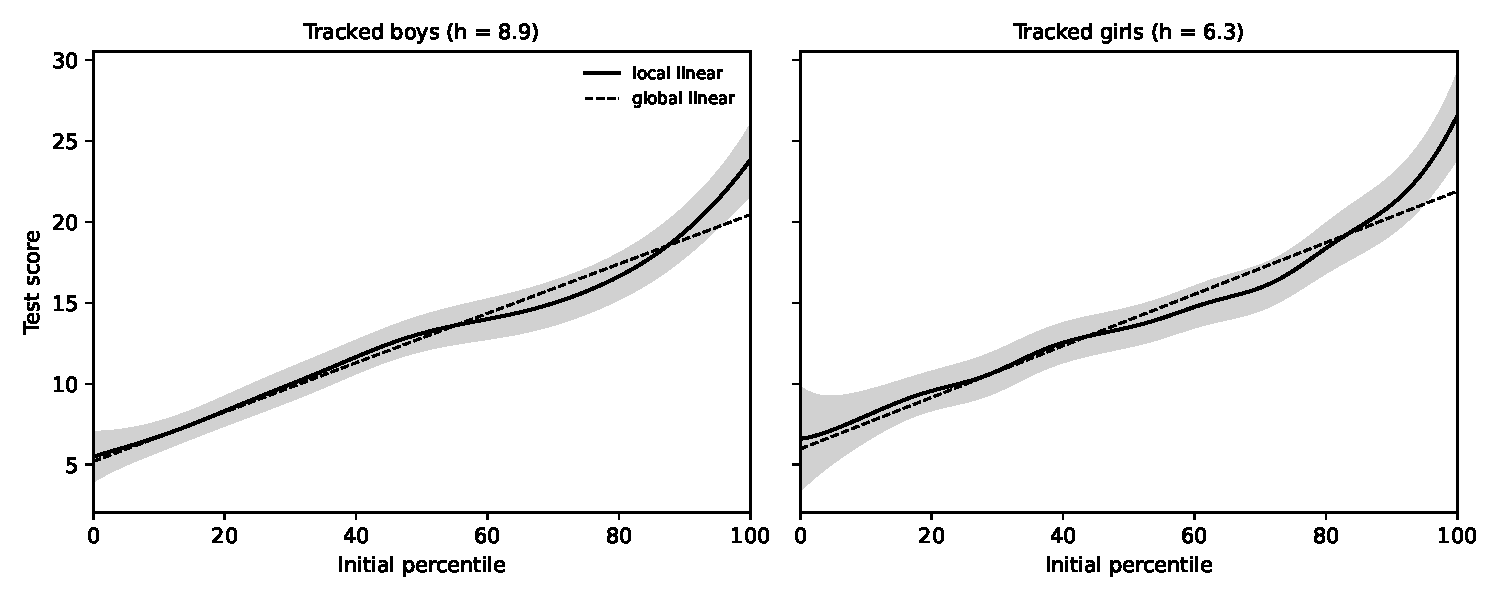
\includegraphics[width=\textwidth]{figures/ch19_07.pdf}
\end{center}
\begin{center}
\small
\begin{tabular}{lccccccc}
\toprule
initial percentile & 0 & 10 & 25 & 50 & 75 & 90 & 100\\
\midrule
boys  & $5.5$ $(0.8)$ & $6.7$ $(0.5)$ & $9.2$ $(0.5)$ & $13.1$ $(0.6)$ & $15.7$ $(0.7)$ & $19.4$ $(0.8)$ & $23.8$ $(1.1)$\\
girls & $6.6$ $(1.7)$ & $8.0$ $(0.8)$ & $10.1$ $(0.6)$ & $13.5$ $(0.6)$ & $17.0$ $(0.7)$ & $21.1$ $(0.9)$ & $26.6$ $(1.4)$\\
\bottomrule
\end{tabular}
\end{center}
\emph{Similarities.}  For both groups the relationship is close to the global linear fit (boys $5.2+0.152x$, girls $6.0+0.159x$)
up to about the 80th percentile, and then becomes convex: students starting at the top gain more than
a linear control predicts.  Clustered standard errors are about $1.5$ times the unclustered ones in both samples.

\emph{Differences.}  The girls' curve lies somewhat above the boys' curve, especially at the top (26.6 versus 23.8 at the
100th percentile), and its upper-tail convexity is stronger (4.6 versus 3.4 points above the linear fit at 100).
The boys' curve is smoother because clustered CV selects a larger bandwidth.  The pointwise bands overlap
almost everywhere, so the gender differences are not statistically decisive.
\end{ex}

%%---------------------------------------------------------------------------
\begin{ex}{19.8}
Men $n=1179$, women $n=640$.  Bandwidths (CV): NW $2.9$ (men), $3.7$ (women); LL $5.0$ (men), $6.0$ (women).  The ROT bandwidths are
$3.2$ and $3.8$.
\begin{center}
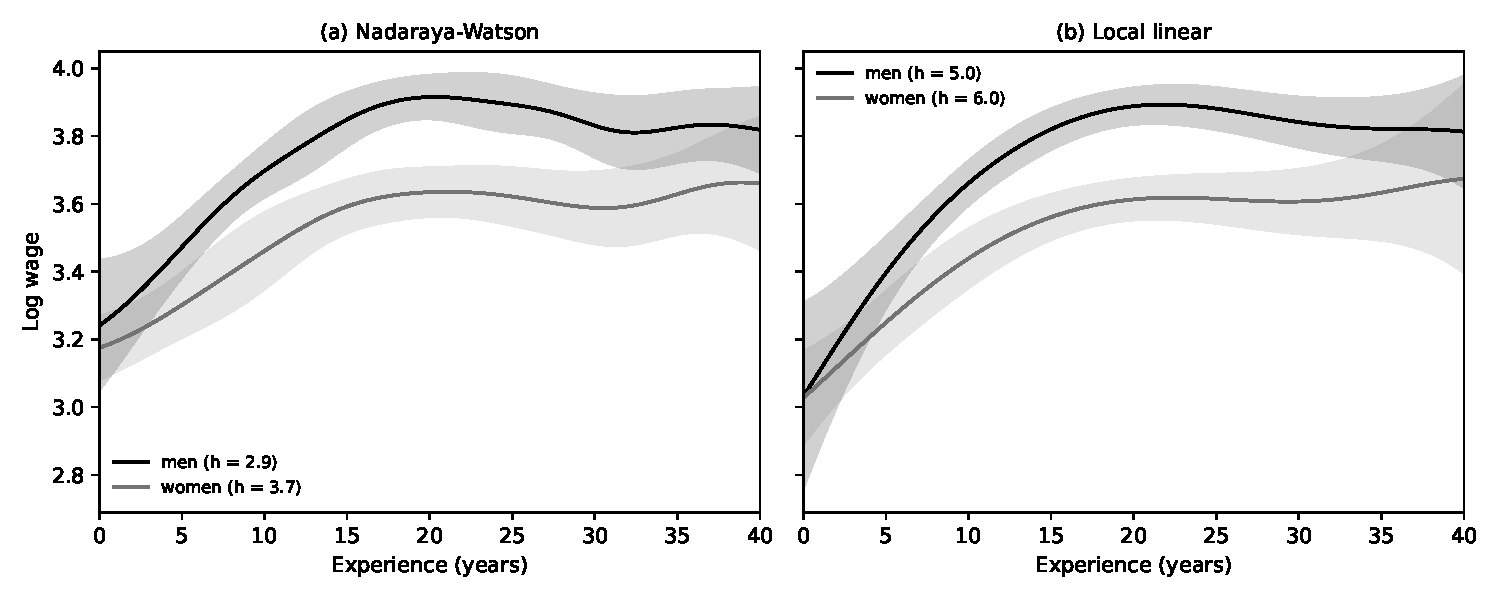
\includegraphics[width=\textwidth]{figures/ch19_08.pdf}
\end{center}
\begin{center}
\small
\begin{tabular}{lccccccc}
\toprule
experience & 0 & 5 & 10 & 20 & 30 & 35 & 40\\
\midrule
men, NW    & $3.24$ $(0.10)$ & $3.47$ $(0.05)$ & $3.70$ $(0.04)$ & $3.92$ $(0.03)$ & $3.83$ $(0.05)$ & $3.83$ $(0.05)$ & $3.82$ $(0.07)$\\
men, LL    & $3.03$ $(0.14)$ & $3.40$ $(0.06)$ & $3.66$ $(0.04)$ & $3.89$ $(0.03)$ & $3.84$ $(0.04)$ & $3.82$ $(0.05)$ & $3.81$ $(0.09)$\\
women, NW  & $3.18$ $(0.05)$ & $3.30$ $(0.05)$ & $3.46$ $(0.06)$ & $3.64$ $(0.04)$ & $3.59$ $(0.06)$ & $3.63$ $(0.06)$ & $3.66$ $(0.10)$\\
women, LL  & $3.03$ $(0.07)$ & $3.25$ $(0.05)$ & $3.44$ $(0.05)$ & $3.61$ $(0.03)$ & $3.61$ $(0.05)$ & $3.63$ $(0.07)$ & $3.67$ $(0.14)$\\
\bottomrule
\end{tabular}
\end{center}
\textbf{(a)}  For both sexes wages rise steeply for the first 15--20 years (by roughly $70$--$85$ log points for men and $45$--$60$
for women, depending on the estimator) and then flatten.  Women earn substantially less than men at every
experience level beyond the first few years, with a gap of about $0.15$--$0.30$ log points.  For men the NW estimate falls by $0.10$ log points
between 20 and 40 years, but the pointwise bands at 20 ($3.92\pm0.07$) and at 30--40 overlap heavily.  For women
there is no decline at all.  The evidence therefore does not support a fall in expected wages after 20 years
for this group: the profile is better described as flat after about 20 years.

\textbf{(b)}  The local linear estimates are smoother (CV selects larger bandwidths) and differ from NW mainly at the
boundaries.  At zero experience LL is $0.15$--$0.2$ lower, because NW is biased upward at a left boundary when
the regression is increasing (Theorem 19.5).  The LL bands are wider at both boundaries (e.g.\ $0.14$ versus $0.10$ at 0 for men,
and $0.14$ versus $0.10$ at 40 for women).  The conclusions are unchanged: rapid growth followed by a plateau, with no
significant decline.
\end{ex}

%%---------------------------------------------------------------------------
\begin{ex}{19.9}
$n=26{,}247$ firm-years ($1934$ firms); the quartiles of $Q$ are $0.40$, $0.73$ and $1.36$.  Because these are panel data, the bands use
standard errors clustered by firm, which are $1.2$--$1.3$ times the unclustered ones.  Bandwidths: $h_{\rm rot}=0.18$.  LL
cross-validation selects $0.10$.  For NW the CV criterion keeps falling down to the smallest bandwidth considered
($h_{\rm rot}/3$), driven by NW's boundary bias at $Q\approx0$, so we use $h_{\rm rot}$ for NW.
\begin{center}
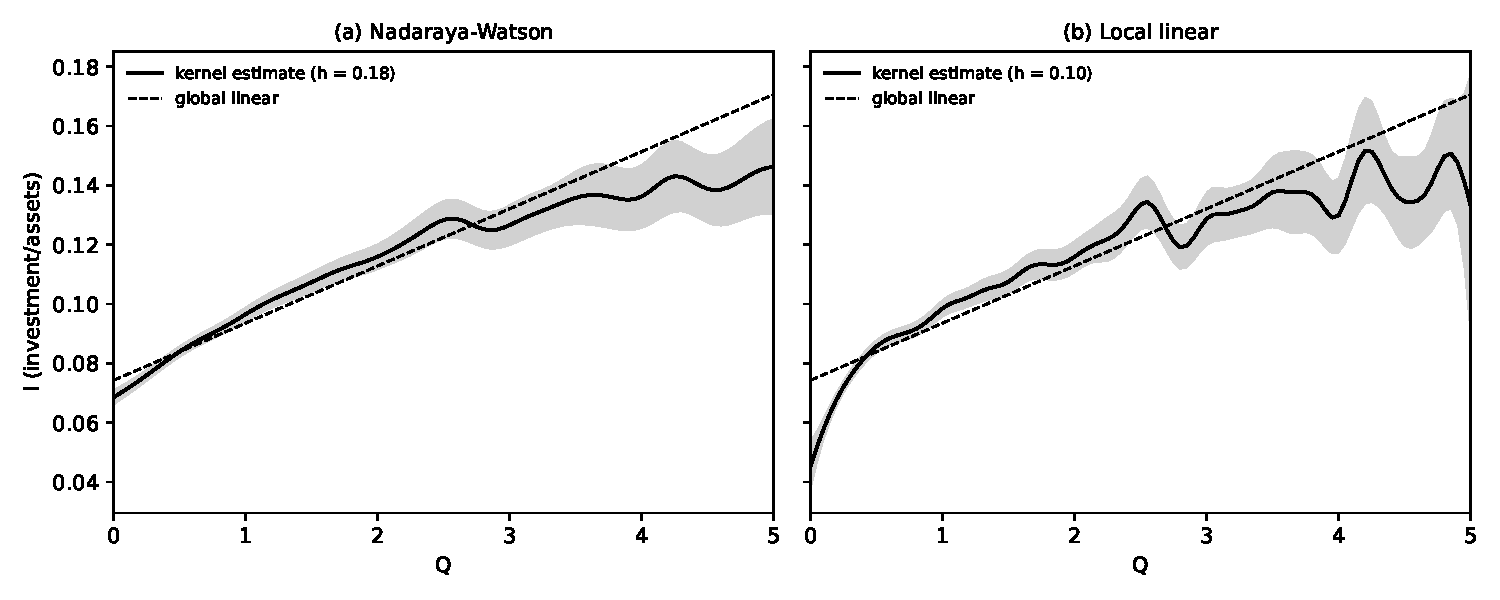
\includegraphics[width=\textwidth]{figures/ch19_09.pdf}
\end{center}
Estimated $\E[I\given Q]$ (clustered s.e.):
\begin{center}
\small
\begin{tabular}{lccccccccc}
\toprule
$Q$ & 0 & 0.25 & 0.5 & 1 & 1.5 & 2 & 3 & 4 & 5\\
\midrule
NW & $0.069$ & $0.076$ & $0.084$ & $0.097$ & $0.107$ & $0.116$ & $0.127$ & $0.136$ & $0.146$\\
LL & $0.045$ & $0.072$ & $0.086$ & $0.099$ & $0.108$ & $0.116$ & $0.129$ & $0.130$ & $0.133$\\
s.e.\ (LL) & $(0.004)$ & $(0.001)$ & $(0.001)$ & $(0.001)$ & $(0.002)$ & $(0.003)$ & $(0.005)$ & $(0.007)$ & $(0.023)$\\
\bottomrule
\end{tabular}
\end{center}
\textbf{(c)}  Yes.  The global linear fit is $I=0.074+0.019Q$.  The local linear estimate is steep for low $Q$ (investment rises by
4 percentage points as $Q$ goes from 0 to $0.5$), has a slope close to $0.02$ between 0.5 and 3, and flattens
above 3.  The linear fit lies outside the (tight) bands near $Q=0$ and for $Q$ above about $3.5$.  Investment is a concave
function of $Q$, in contrast to the linear specification implied by the $Q$ theory of investment.  (The NW estimate
misses the steep initial segment because of boundary bias.  Its CV preference for ever-smaller
bandwidths is a symptom of exactly this.)
\end{ex}

%%---------------------------------------------------------------------------
\begin{ex}{19.10}
$n=219$.  Debt/GDP ranges from $0$ to $121\%$ but exceeds 90\% in only six years (1944--1949).  Bandwidths: $h_{\rm rot}=13.4$; CV selects
$24.0$ for NW and $37.1$ for LL.
\begin{center}
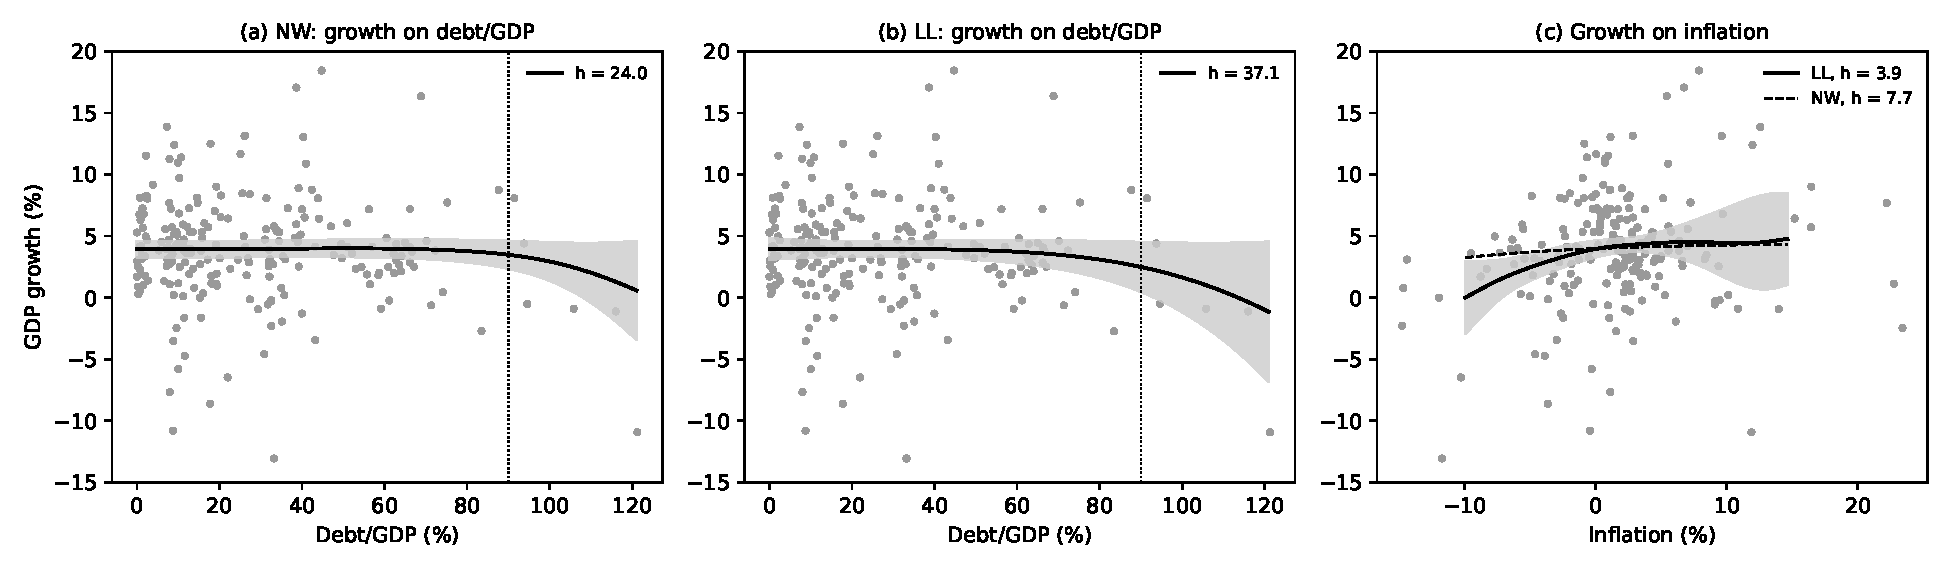
\includegraphics[width=\textwidth]{figures/ch19_10.pdf}
\end{center}
\textbf{(a)--(b)}  Both estimates are flat at about $3.9$--$4.0\%$ growth for debt ratios up to 50--60\%.  Above that they decline:
NW $3.78\ (0.46)$ at 80\%, $3.48\ (0.57)$ at 90\%, $2.94\ (0.79)$ at 100\%; LL $3.09\ (0.76)$ at 80\%, $2.49\ (1.03)$ at 90\%, $1.64\ (1.43)$ at 100\%.  The pointwise bands
widen rapidly above 80\%.

\textbf{(c)}  There is weak evidence of a decline in growth at high debt levels, but no evidence of a break at 90\%.
The estimated decline is gradual (a smooth kernel fit cannot show a threshold, and there is no visible
jump in the data), and the difference between growth at 30\% and at 90\% debt is well within sampling error.
Most importantly, the high-debt observations are the six post-war years 1944--1949, when output fell as
wartime production was unwound (average growth $-0.2\%$ versus $4.0\%$ in all other years).  The negative association at
high debt reflects this single episode, whose causality runs from war to both debt and the post-war
output contraction, not from debt to growth.

\textbf{(d)}  Growth on inflation: NW ($h=7.7$) rises gently from $3.2\%$ at $-10\%$ inflation to $4.3\%$ at $15\%$.  LL (the CV minimizer is at the grid
boundary, so $h_{\rm rot}=3.9$ is used) shows the shape more clearly: $2.5\ (0.5)$ at $-5\%$, $4.0\ (0.3)$ at $0\%$, $4.2$ at $2\%$, $4.5$ at $5\%$.  Deflation years
are associated with markedly lower growth.  Above about $5\%$ inflation the estimate is flat and imprecise.  The
deflation--low growth association comes largely from 19th-century and early-20th-century depressions.  It is a
correlation in a nonstationary historical sample, not a causal effect of inflation.
\end{ex}

%%---------------------------------------------------------------------------
\begin{ex}{19.11}
$n=234$ quarterly observations (1959Q3--2017Q4), mean annualized growth $3.1\%$.  Evaluation region: the 2.5--97.5\% quantiles of
$Y_{t-1}$, $[-4.3,\,9.4]$.  Bandwidths: $h_{\rm rot}=3.44$.  CV selects $2.22$ for NW, while for LL the CV criterion is minimized at the largest
bandwidth considered ($3h_{\rm rot}$), i.e.\ it prefers an essentially linear fit, so $h_{\rm rot}$ is used for the plot.
\begin{center}
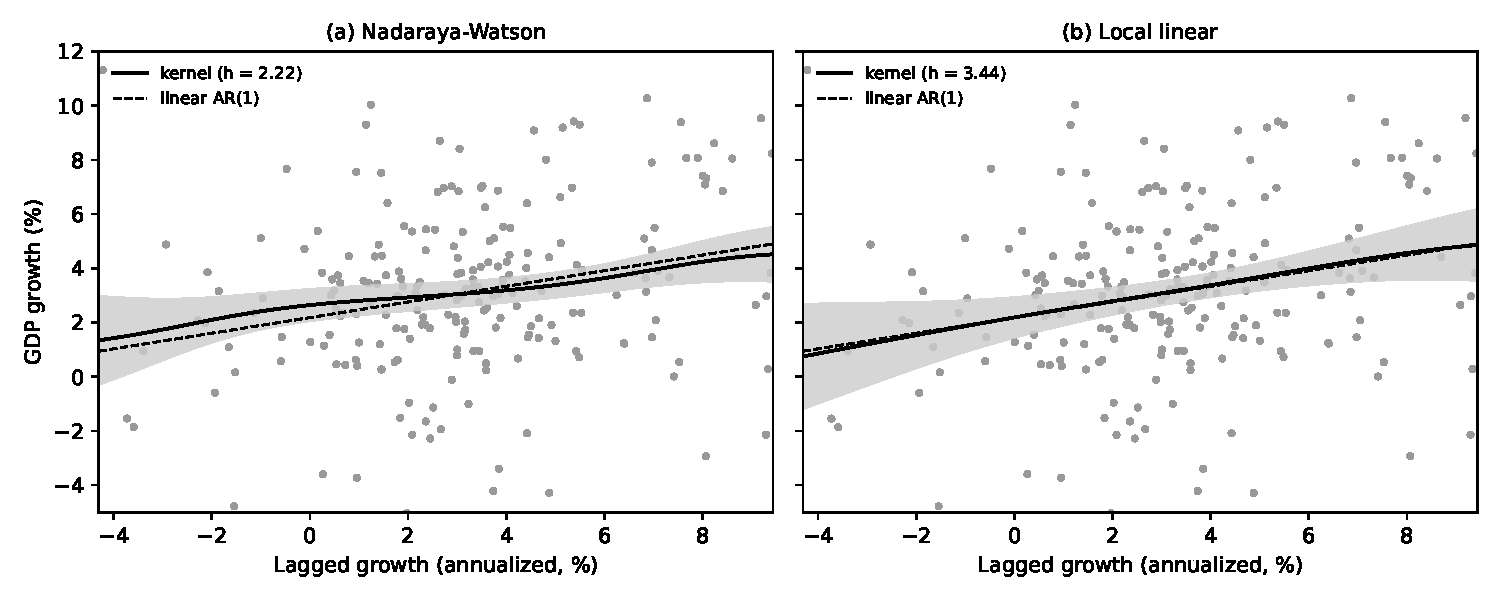
\includegraphics[width=\textwidth]{figures/ch19_11.pdf}
\end{center}
Estimates of $m(x)$ (s.e.): NW $2.10\ (0.42)$ at $x=-2$, $2.64\ (0.29)$ at 0, $3.04\ (0.23)$ at 3, $3.64\ (0.25)$ at 6, $4.24\ (0.38)$ at 8; LL $1.54\ (0.62)$, $2.19\ (0.37)$,
$3.08\ (0.22)$, $3.99\ (0.31)$, $4.56\ (0.50)$ at the same points.  The linear AR(1) is $\wh Y_t=2.18+0.288Y_{t-1}$.

\textbf{(d)}  No.  Both kernel estimates are close to the linear AR(1) line, which lies inside the 95\% bands over the
whole range.  Cross-validation for the local linear estimator prefers the largest bandwidth, i.e.\ linearity.
The NW estimate is slightly flatter in the middle and steeper at the extremes, but the deviations are small
relative to the bands.  With 234 observations there is no detectable nonlinearity in the conditional mean of
U.S.\ GDP growth.  Asymmetries between recessions and expansions, if present, are not captured by a
nonlinear function of last quarter's growth alone.
\end{ex}

%% ===========================================================================
%% Chapter 20. Series Regression
%% ===========================================================================
\solchapter{20}{Series Regression}

\begin{center}
\begin{minipage}{0.86\textwidth}
\small
Solutions to all 18 exercises of Chapter 20 of Bruce E.\ Hansen, \emph{Econometrics}
(Princeton University Press, 2022).  The empirical exercises use \texttt{cps09mar}, \texttt{RR2010}, \texttt{DDK2011},
\texttt{CHJ2004} and \texttt{AL1999}.  Following Section 20.18, standard errors are HC3 (computed from leave-one-out
prediction errors), or delete-cluster versions for clustered data.  Cross-validation is the leave-one-out
criterion $\text{CV}=n^{-1}\sum\wt e_i^{2}$ (Section 20.17).  As a check, the Angrist--Lavy reading-score NPIV estimates of Table 20.1,
the Wald statistic $12.7$ ($p=0.013$) and the effect $-2.96\ (1.21)$ are reproduced exactly.  Figures are in \texttt{figures/}.
\end{minipage}
\end{center}

\bigskip
\hrule
\bigskip

%%---------------------------------------------------------------------------
\begin{ex}{20.1}
For $X>2$ both spline terms are active, so the slope is $2+5-3=4$.  (For $X<1$ it is $2$; for $1<X<2$ it is $7$.)
\end{ex}

%%---------------------------------------------------------------------------
\begin{ex}{20.2}
$m_K$ is continuous and piecewise linear with slopes $\beta_1$ on $(-\infty,\tau_1)$, $\beta_1+\beta_2$ on $(\tau_1,\tau_2)$, $\beta_1+\beta_2+\beta_3$ on $(\tau_2,\tau_3)$ and
$\beta_1+\beta_2+\beta_3+\beta_4$ on $(\tau_3,\infty)$.  A continuous piecewise-linear function is non-decreasing iff every slope is non-negative:
\[
  \beta_1\ge0,\qquad \beta_1+\beta_2\ge0,\qquad \beta_1+\beta_2+\beta_3\ge0,\qquad \beta_1+\beta_2+\beta_3+\beta_4\ge0 .
\]
(On a bounded support $[a,b]\ni\tau_1,\tau_2,\tau_3$ the same four conditions apply.)
\end{ex}

%%---------------------------------------------------------------------------
\begin{ex}{20.3}
A continuous piecewise-linear function is concave iff its slopes are non-increasing, i.e.\ each change of slope
at a knot is non-positive:
\[
  \beta_2\le0,\qquad \beta_3\le0,\qquad \beta_4\le0,
\]
with $\beta_0,\beta_1$ unrestricted.
\end{ex}

%%---------------------------------------------------------------------------
\begin{ex}{20.4}
(The book prints $\beta_2x^{3}$; for a quadratic spline the term is $\beta_2x^{2}$.)  The function is continuously differentiable, and
its second derivative is piecewise constant:
\[
  m_K''(x)=\begin{cases}2\beta_2, & x<\tau_1,\\ 2(\beta_2+\beta_3), & \tau_1<x<\tau_2,\\ 2(\beta_2+\beta_3+\beta_4), & \tau_2<x<\tau_3,\\ 2(\beta_2+\beta_3+\beta_4+\beta_5), & x>\tau_3.\end{cases}
\]
A $C^{1}$ function with piecewise continuous second derivative is concave iff $m''\le0$ wherever it exists:
\[
  \beta_2\le0,\qquad \beta_2+\beta_3\le0,\qquad \beta_2+\beta_3+\beta_4\le0,\qquad \beta_2+\beta_3+\beta_4+\beta_5\le0 .
\]
(With the literal cubic term, $m''$ is linear within each segment.  Concavity then requires $m''\le0$ at both endpoints of
every segment of the support; on an unbounded support it forces $\beta_2=0$.)
\end{ex}

%%---------------------------------------------------------------------------
\begin{ex}{20.5}
Take the linear spline regressor $(X-\tau)\indic\{X\ge\tau\}$.  If $\tau\ge\max_iX_i$ it equals zero for every observation, so the design
matrix has a zero column and its coefficient is not identified.  If $\tau\le\min_iX_i$ it equals $X_i-\tau$ for every observation, an
exact linear combination of the intercept and $X_i$: perfect collinearity again.  The same holds for
higher-order splines: below the support $(X-\tau)^{p}$ is a polynomial of degree $p$ already spanned by $1,X,\dots,X^{p}$.  In
either case $\bs X'\bs X$ is singular and OLS cannot be computed (software drops the variable).  The knot adds
flexibility only by splitting the sample, so it must lie strictly inside the support, with enough
observations on both sides to estimate the change in slope precisely.
\end{ex}

%%---------------------------------------------------------------------------
\begin{ex}{20.6}
\textbf{(a)}  $\wh m_K'(x)=\wh\beta_1+2\wh\beta_2x+3\wh\beta_3x^{2}+\cdots+p\wh\beta_px^{p-1}$.

\textbf{(b)}  Yes: $\wh m_K'(x)=a_K(x)'\wh\beta_K$ with $a_K(x)=(0,1,2x,\dots,px^{p-1})'$.  The functional $\theta=a(m)=m'(x)$ is linear in $m$.

\textbf{(c)}  By Theorem 20.8, with $K=p+1$ and $r_K=m-m_K$,
\[
  \frac{\sqrt n\bigl(\wh m_K'(x)-m'(x)+r_K'(x)\bigr)}{V_K^{1/2}}\convd N(0,1),\qquad V_K=a_K(x)'Q_K^{-1}\Omega_KQ_K^{-1}a_K(x).
\]
The bias is the derivative of the approximation error, $r_K'(x)$.

\textbf{(d)}  With $\wh V_{\wh\beta}$ the HC3 covariance matrix (20.32), $s(\wh m_K'(x))=\sqrt{a_K(x)'\wh V_{\wh\beta}a_K(x)}$, and a 95\% pointwise interval is
$\wh m_K'(x)\pm1.96\,s(\wh m_K'(x))$.  As for $\wh m_K(x)$, the interval ignores the bias $r_K'(x)$: it is valid under undersmoothing, or
as an interval for the pseudo-true derivative.  Derivatives are estimated less precisely than levels,
especially near the boundary, where $|a_K(x)|$ is large.
\end{ex}

%%---------------------------------------------------------------------------
\begin{ex}{20.7}
$\text{CV}(K)=n^{-1}\sum_i\wt e_i^{2}$ with $\wt e_i=\wh e_i/(1-h_{ii})$.
\begin{itemize}[leftmargin=*]
\item \emph{Rescaling $Y$ to $cY$} multiplies every residual and prediction error by $c$ and leaves the leverages unchanged.
So $\text{CV}(K)$ is multiplied by $c^{2}$ for every $K$ and the minimizing $K$ is unchanged.
\item \emph{Rescaling $X$ to $cX$}: for polynomials, $\{1,cX,\dots,(cX)^{p}\}$ spans the same space as $\{1,X,\dots,X^{p}\}$.  The same is true for
splines when the knots are rescaled with $X$ ($(cX-c\tau)^{p}=c^{p}(X-\tau)^{p}$).  Fitted values, residuals and leverages are unchanged,
so the CV function and its minimizer are unchanged.  (If spline knots are kept fixed in the original
units while $X$ is rescaled, the model itself changes.)
\end{itemize}
Scaling does matter numerically: rescaling $X$ to $[0,1]$ reduces the ill-conditioning of high-order
polynomial designs, which is why the exercises below do it.
\end{ex}

%%---------------------------------------------------------------------------
\begin{ex}{20.8}
Write $e_K=e+r_K(X)$ with $r_K(x)=m(x)-X_K(x)'\beta_K$ the approximation error.

\textbf{(a)}  In general no: $\E[e_K\given Z]=\E[e\given Z]+\E[r_K(X)\given Z]=\E[r_K(X)\given Z]$, which is non-zero because $X$ depends on $Z$ (relevance) and
$r_K\ne0$ unless $m$ lies exactly in the span of $X_K$.

\textbf{(b)}  Yes, if $\E[Z_KX_K']$ is non-singular: define $\beta_K=\E[Z_KX_K']^{-1}\E[Z_KY]$.  Then $\E[Z_Ke_K]=\E[Z_KY]-\E[Z_KX_K']\beta_K=0$ by construction.
This is the just-identified IV projection coefficient; its approximation error need not be small in any
$L_2$ sense.

\textbf{(c)}  In general no.  $\E[Z_Le_K]=\E[Z_Lm(X)]-\E[Z_LX_K']\beta_K$ is $L$ equations in $K<L$ unknowns.  They have a solution only if
$\E[Z_Lm(X)]$ lies in the column space of $\E[Z_LX_K']$, e.g.\ if $r_K\equiv0$.  With a genuine approximation error the
overidentifying restrictions fail.  $\beta_K$ can then only be defined as a pseudo-true GMM value that makes
$\E[Z_Le_K]$ as small as possible, and overidentification tests will tend to reject for small $K$.
\end{ex}

%%---------------------------------------------------------------------------
\begin{ex}{20.9}
$n=50{,}742$.  Experience ($\text{age}-\text{education}-6$) ranges from $-4$ to $75$ and is rescaled as $(x-\min)/(\max-\min)$.
\begin{center}
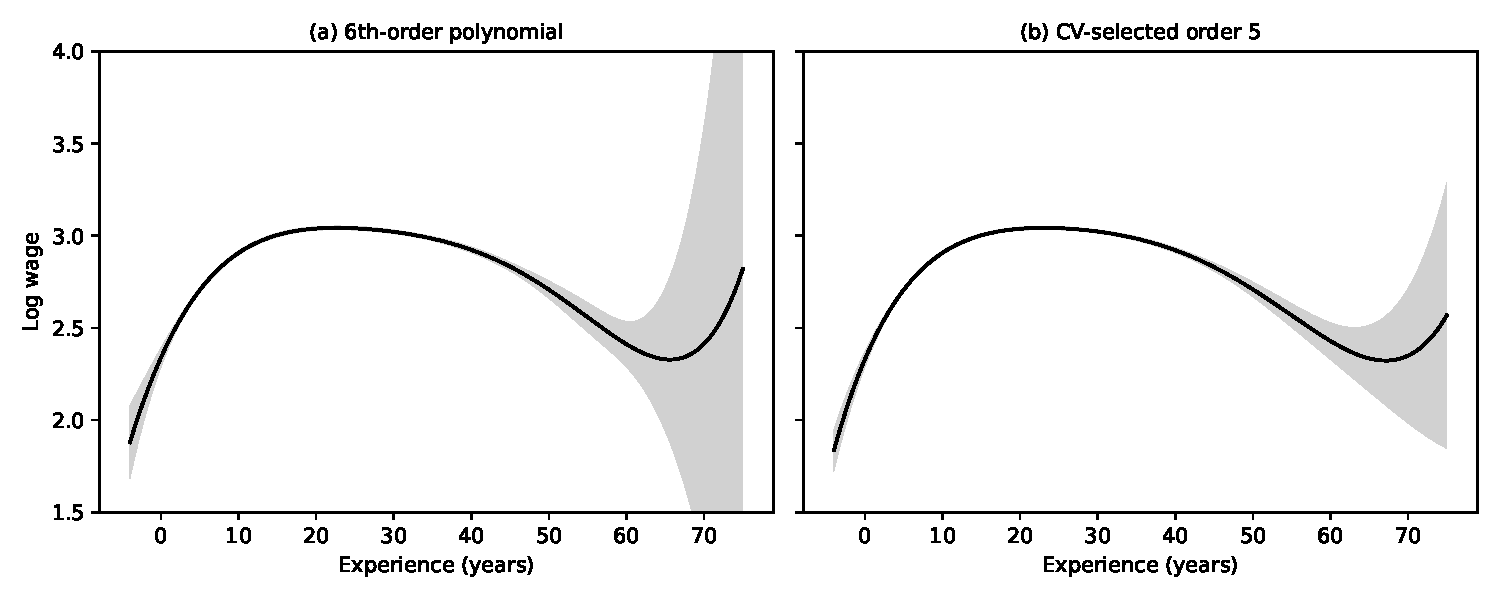
\includegraphics[width=\textwidth]{figures/ch20_09.pdf}
\end{center}
Selected values of the 6th-order fit (s.e.): $2.34\ (0.03)$ at 0 years, $2.91\ (0.006)$ at 10, $3.04\ (0.005)$ at 20, $3.02\ (0.005)$ at 30,
$2.92\ (0.008)$ at 40, $2.71\ (0.02)$ at 50, $2.41\ (0.06)$ at 60, $2.33\ (0.20)$ at 65 and $2.41\ (0.61)$ at 70.

\textbf{(c)}  Log wages rise steeply over the first ten years (by about 57 log points), flatten around 20--30 years, and decline
after about 35 years, by roughly 60 log points by 60 years of experience.  This is a concave profile,
similar to but more flexible than the quadratic Mincer specification.  Above about 60 years the estimate turns
\emph{up} again, but this is not credible.  Only 3 of the $50{,}742$ workers have more than 65 years of experience (and 25 more than
60), so the polynomial is determined almost entirely by its behaviour elsewhere.  The pointwise band
widens explosively (the s.e.\ at 70 is $0.6$, i.e.\ $\pm120$ log points).  The upturn is a boundary artefact of a global
polynomial with a large regressor norm $\zeta_K(x)$ at the edge of the support (Section 20.18).  No conclusion should be
drawn for experience above about 60.
\end{ex}

%%---------------------------------------------------------------------------
\begin{ex}{20.10}
\begin{center}
\small
\begin{tabular}{lcccccccc}
\toprule
order & 1 & 2 & 3 & 4 & 5 & 6 & 7 & 8\\
\midrule
CV & $0.45408$ & $0.44027$ & $0.43921$ & $0.43891$ & $\mathbf{0.43878}$ & $0.43886$ & $0.43892$ & $0.43878$\\
AIC$+41000$ & $940.0$ & $-627.9$ & $-749.3$ & $-785.3$ & $\mathbf{-798.9}$ & $-797.4$ & $-796.4$ & $-798.0$\\
\bottomrule
\end{tabular}
\end{center}
\textbf{(a)}  Both criteria select order 5 (order 8 is a near tie), a large improvement over the quadratic.

\textbf{(b)}  The order-5 estimate is shown in panel (b) of the figure in Exercise 20.9.  It is practically identical to the
order-6 fit up to 60 years of experience.  Its bands are narrower at the upper boundary (s.e.\ $0.09$ at 65 and $0.19$ at
70), and the spurious upturn is milder.  The interpretation is unchanged: rapid early growth, a peak around 20--25
years ($\approx3.04$), and a gradual decline.
\end{ex}

%%---------------------------------------------------------------------------
\begin{ex}{20.11}
Education ranges from 0 to 20 years but takes only a few distinct values (0, 4, 6, 8, 9, \dots, 14, 16, 18, 20).
\begin{center}
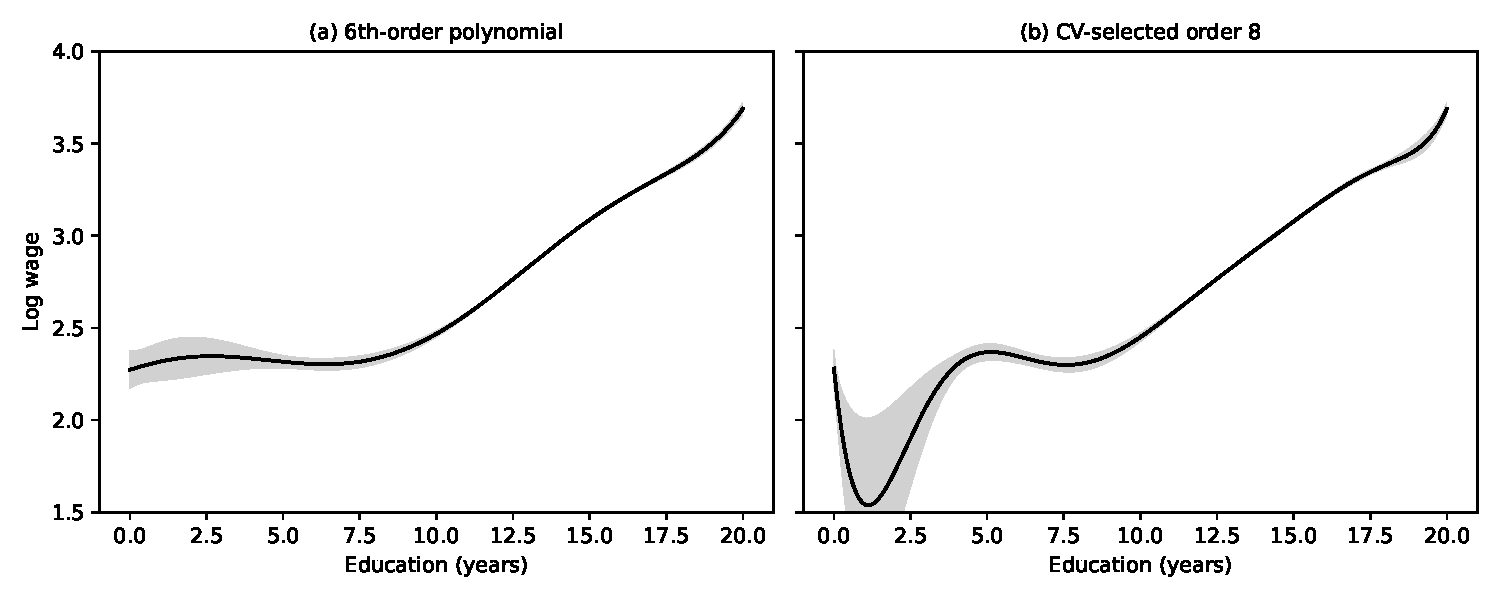
\includegraphics[width=\textwidth]{figures/ch20_11.pdf}
\end{center}
Fitted values (s.e.): $2.27\ (0.05)$ at 0, $2.33\ (0.03)$ at 4, $2.33\ (0.02)$ at 8, $2.47\ (0.01)$ at 10, $2.70\ (0.004)$ at 12, $2.96\ (0.004)$ at 14,
$3.20\ (0.005)$ at 16, $3.38\ (0.008)$ at 18 and $3.69\ (0.02)$ at 20.  The return to schooling is essentially zero below 8 years and about $10$--$15\%$ per year above 10
years.  This is the convex profile seen in earlier chapters.  Precision is lowest at low education, where there are few
workers.
\end{ex}

%%---------------------------------------------------------------------------
\begin{ex}{20.12}
CV $\times10^{5}$ for orders 1--8: $36868$, $36623$, $36563$, $36563$, $36514$, $36511$, $36512$, $\mathbf{36507}$; AIC is also minimized at order 8.  The criterion
keeps falling, slightly, up to the largest order considered, though orders 5--8 are within $0.02\%$ of each other.
The order-8 estimate (panel (b) above) is very close to the order-6 fit: flat below 8 years and steep
and convex above.  With so few distinct values of education, high-order polynomials are close to
fitting a separate mean for each education level.
\end{ex}

%%---------------------------------------------------------------------------
\begin{ex}{20.13}
\begin{center}
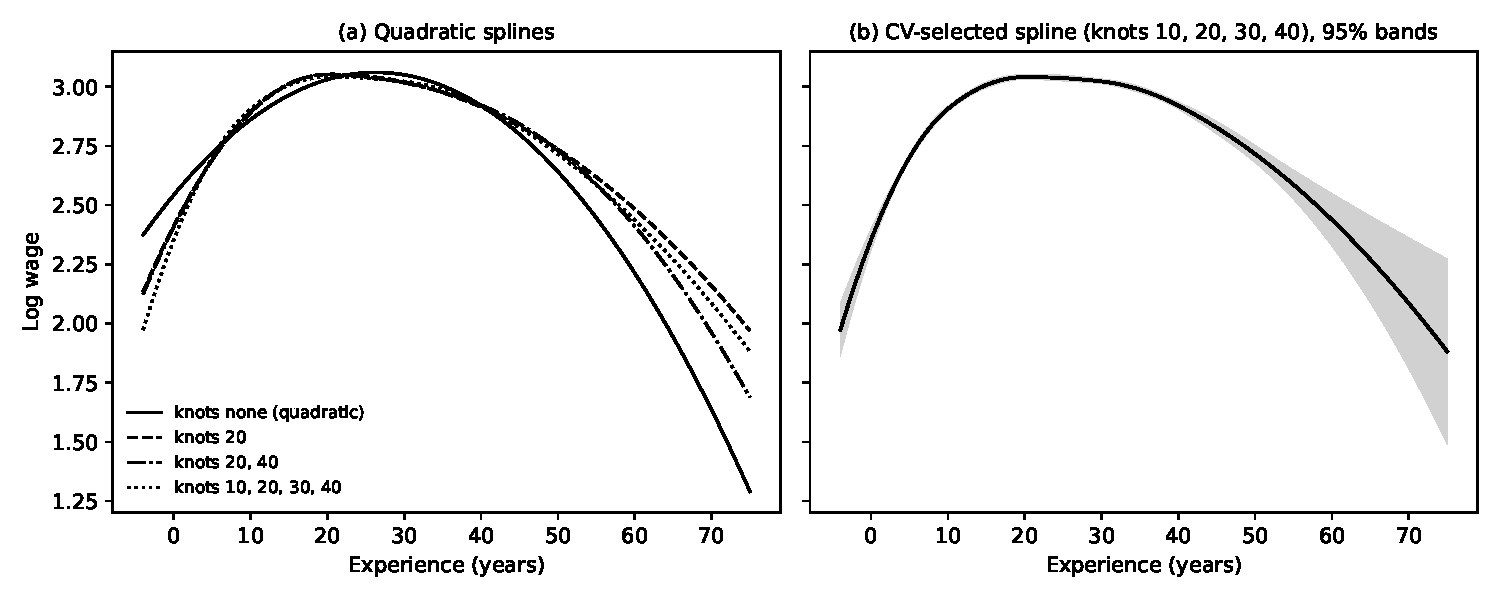
\includegraphics[width=\textwidth]{figures/ch20_13.pdf}
\end{center}
\textbf{(a)}  All four agree between about 5 and 45 years: a peak of $\approx3.04$--$3.05$ around 20--25 years.  The quadratic is too
rigid.  It overstates wages at zero experience ($2.54$ versus $2.35$--$2.41$ for the splines) and forces an
accelerating decline (to $1.64$ at 70 years).  The spline models allow a steep early rise followed by a flat
middle section.

\textbf{(b)}  CV: $0.44027$ (quadratic), $0.43891$ (knot 20), $0.43891$ (knots 20, 40), $\mathbf{0.43882}$ (knots 10, 20, 30, 40).  AIC ($+41000$):
$-627.9$, $-784.2$, $-784.9$, $\mathbf{-795.2}$.  Both select the four-knot spline.

\textbf{(c)}  The four-knot spline (right panel) rises from $2.35$ at 0 to $3.04$ at 20 years, is flat to 30 years, and declines to
$2.72$ at 50 and $2.44$ at 60.  The bands are tight except at the boundaries.

\textbf{(d)}  The order-5 polynomial has a marginally smaller CV ($0.43878$ versus $0.43882$), but the difference is negligible.  The
spline is preferable for interpretation and extrapolation: it does not produce the implausible upturn
beyond 60 years that the polynomials show, because each quadratic piece depends only locally on the
data.
\end{ex}

%%---------------------------------------------------------------------------
\begin{ex}{20.14}
\begin{center}
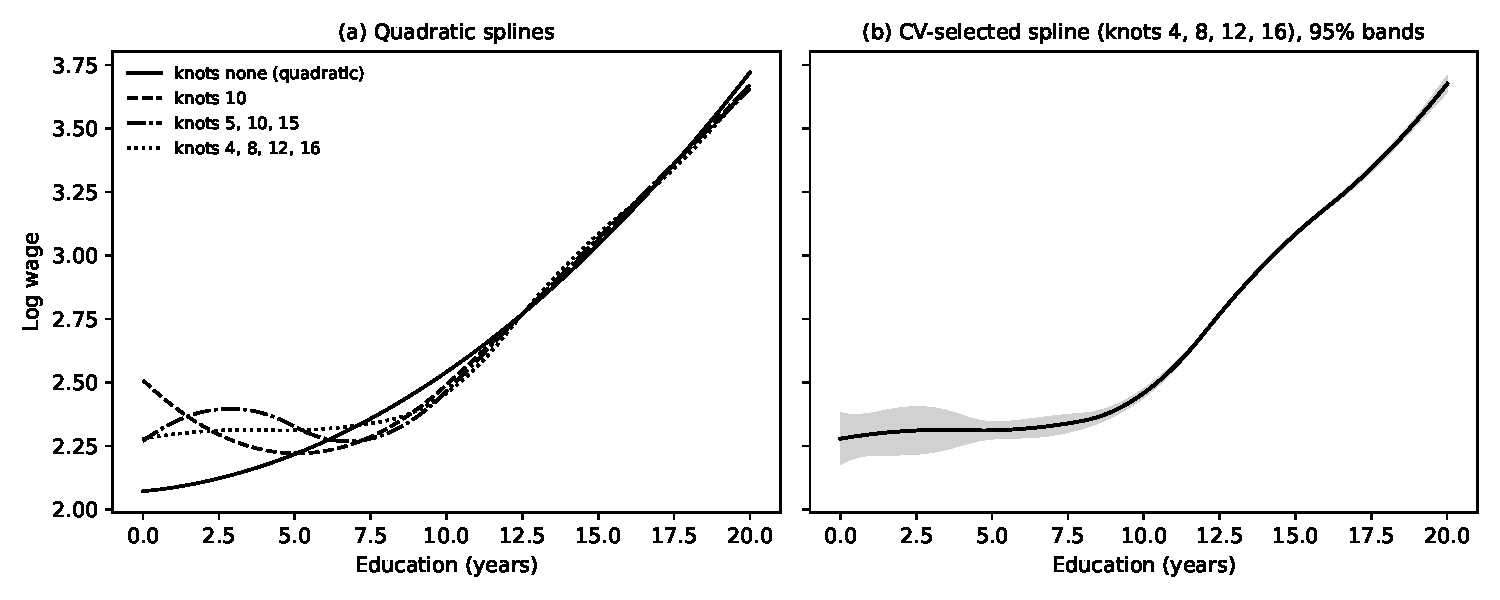
\includegraphics[width=\textwidth]{figures/ch20_14.pdf}
\end{center}
\textbf{(a)}  The quadratic is smooth and convex but misses the flat segment at low education; the one-knot spline
overshoots at 0 years ($2.51$).  The three- and four-knot splines capture a flat profile up to 8 years and a steep,
roughly linear-convex rise afterwards.

\textbf{(b)}  CV: $0.36623$, $0.36559$, $0.36535$, $\mathbf{0.36516}$; AIC ($+51000$): $30.0$, $-58.4$, $-91.6$, $\mathbf{-117.6}$.  The four-knot spline is selected.

\textbf{(c)}  Selected fit (s.e.): $2.31\ (0.03)$ at 4, $2.35\ (0.02)$ at 8, $2.70\ (0.004)$ at 12, $2.97\ (0.005)$ at 14, $3.19\ (0.005)$ at 16, $3.40\ (0.007)$ at 18 and
$3.68\ (0.02)$ at 20.  Returns are near zero through primary school and about $11$--$14\%$ per year above 10 years.

\textbf{(d)}  The order-8 polynomial has a slightly lower CV ($0.36507$ versus $0.36516$), so by CV the polynomial wins
narrowly.  The two fits are visually indistinguishable where the data are dense.  Given only a dozen
distinct education values, either is acceptable; a set of education dummies would be the natural
saturated alternative.
\end{ex}

%%---------------------------------------------------------------------------
\begin{ex}{20.15}
$n=218$ (1792--2009).  Estimates, with HC3 standard errors:
\begin{center}
\small
\begin{tabular}{lcccc}
\toprule
 & $\wh\alpha$ & slope of $m$, segment 1 & segment 2 & segment 3\\
\midrule
(1) linear & $0.300$ $(0.092)$ & $-0.008$ $(0.014)$ & & \\
(2) knot at 60 & $0.284$ $(0.093)$ & $0.010$ $(0.014)$ & $-0.076$ $(0.070)$ & \\
(3) knots at 40, 80 & $0.280$ $(0.094)$ & $0.034$ $(0.025)$ & $-0.053$ & $-0.071$\\
\midrule
CV & \multicolumn{4}{l}{$18.29$ (1), $18.41$ (2), $18.60$ (3); \quad AIC: $631.1$, $630.1$, $630.0$}\\
\bottomrule
\end{tabular}
\end{center}
\begin{center}
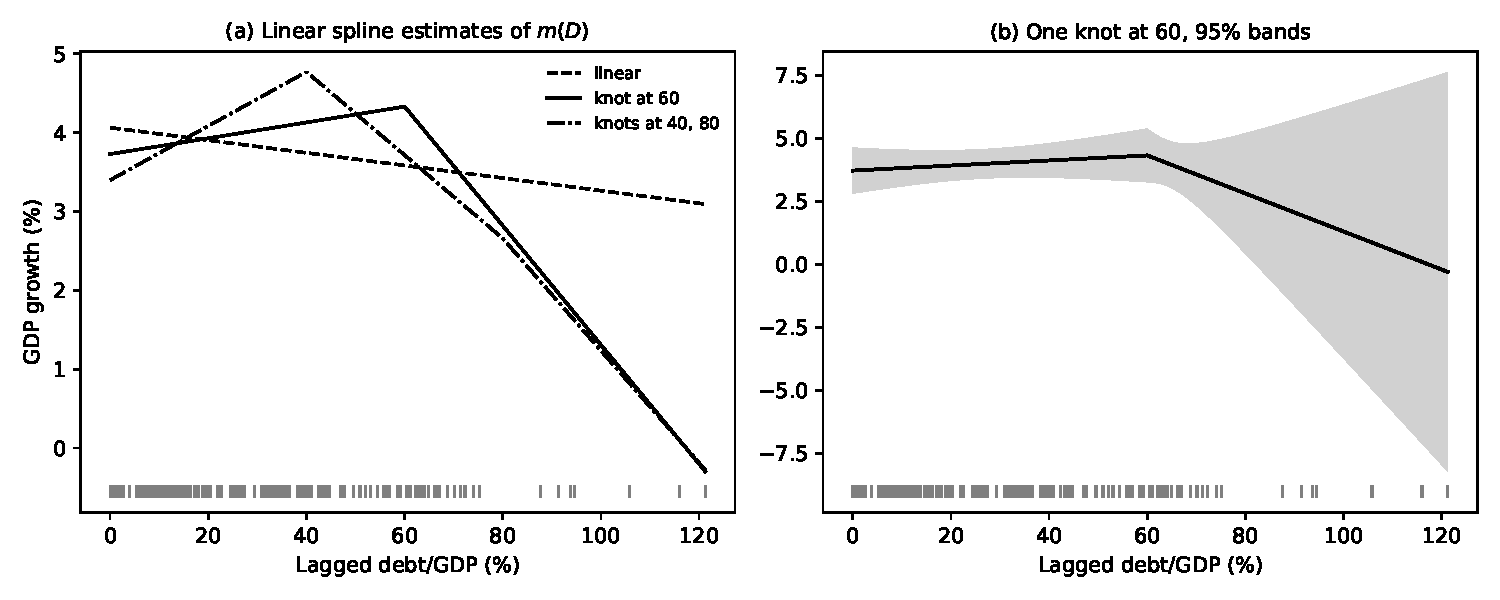
\includegraphics[width=\textwidth]{figures/ch20_15.pdf}
\end{center}
\textbf{(c)}  CV prefers the linear model; AIC prefers the spline models by a trivial margin (about $1$ point).  With no
decisive evidence, the simplest model is preferred.

\textbf{(d)}  There is no significant evidence that debt affects subsequent growth.  In the linear model the slope is
$-0.008$ percentage points of growth per point of debt/GDP ($t=-0.6$).  In the one-knot model the slope above 60\% is
$-0.076\ (0.070)$, negative but insignificant, and the band in panel (b) is very wide above 60.  The apparent
``kink'' is driven by only seven observations with debt above 80\%: 1944--1950, the post-war demobilization,
when output fell as military spending was cut.  That episode is a special historical event rather than
evidence of a general threshold at 90\%.  U.S.\ data alone cannot support the Reinhart--Rogoff claim.
\end{ex}

%%---------------------------------------------------------------------------
\begin{ex}{20.16}
We use the raw total score (\emph{totalscore}, as in Section 19.21); $n=5304$ pupils in $111$ schools.
\begin{center}
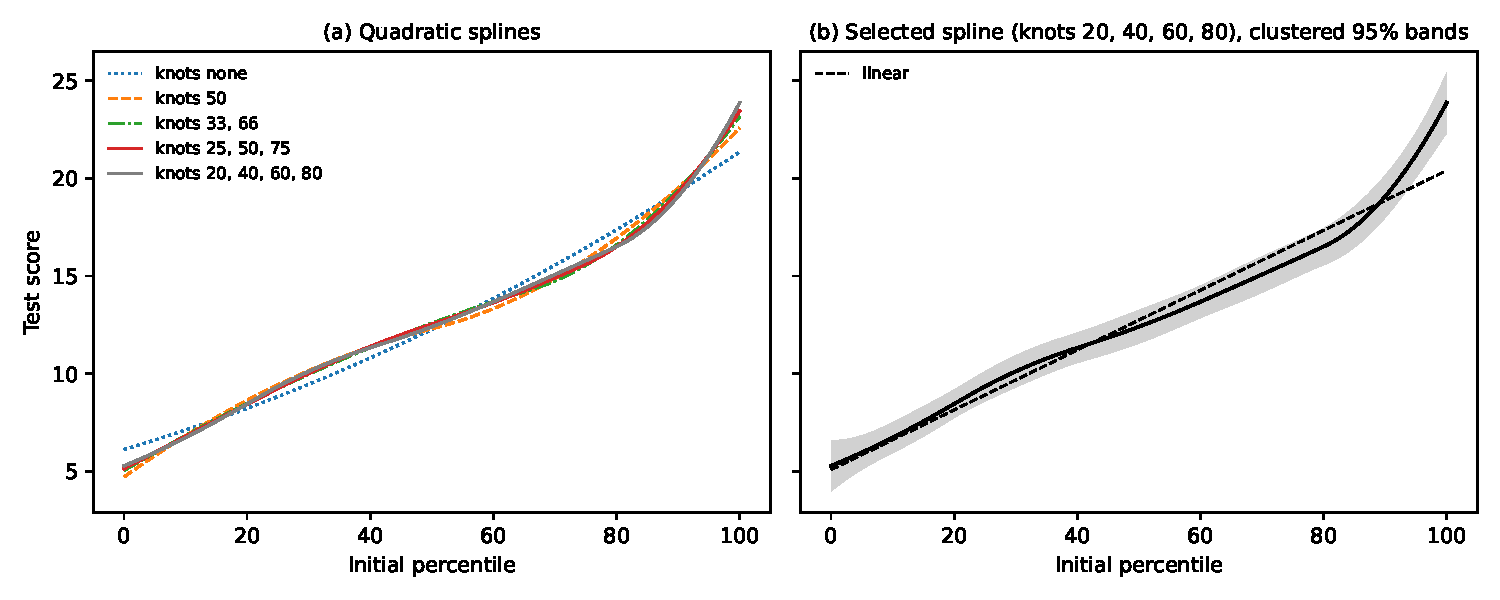
\includegraphics[width=\textwidth]{figures/ch20_16.pdf}
\end{center}
\textbf{(a)}  All specifications agree: scores rise with the initial percentile, roughly linearly up to about 80
and more steeply above.  The pure quadratic differs slightly at the extremes.

\textbf{(b)}  Leave-school-out CV: $63.244$, $62.954$, $62.932$, $62.924$, $\mathbf{62.923}$ (conventional CV and AIC give the same ranking up to ties).  Any
knot improves on the quadratic, and the models with three or four knots are essentially tied.  We select the four-knot
spline, the CV minimizer, noting that the three-knot model is practically equivalent.

\textbf{(c)}  Fitted scores (clustered s.e.): $5.3\ (0.7)$ at percentile 0, $6.7\ (0.4)$ at 10, $9.3\ (0.4)$ at 25, $12.4\ (0.4)$ at 50, $15.8\ (0.5)$ at 75,
$19.1\ (0.6)$ at 90 and $23.9\ (0.8)$ at 100.  The slope is about $0.13$ points per percentile in the middle of the distribution, rising
to about $0.2$ between the 75th and 90th percentiles and about $0.5$ in the top decile.  Students who start at the top of the distribution gain more than a linear control
would predict, the same conclusion as the kernel analysis of Section 19.21.  A linear specification of the
percentile control, as in Duflo, Dupas and Kremer, is adequate except in the top quintile.
\end{ex}

%%---------------------------------------------------------------------------
\begin{ex}{20.17}
$n=8684$ households; income is rescaled to units of $100{,}000$ pesos.  Orders 1--12 were compared by CV.
\begin{itemize}[leftmargin=*]
\item \textbf{(a)} No controls: CV is minimized at order 11 (orders 10 and 11 are virtually tied; order 12 and higher
deteriorate sharply as the design becomes ill-conditioned).
\item \textbf{(b)} Paper's 15 controls (education dummies, age, female, married, children, household size, employment
status): CV selects order 6 (AIC 7).
\item \textbf{(c)} A smaller demographic set (age, female, married, size, both-work, not-employed): CV selects order 7.  Its
best CV ($3.333\times10^{8}$) is worse than with the full control set ($3.060\times10^{8}$; no controls: $3.824\times10^{8}$), so the paper's
controls are preferred by CV.
\end{itemize}
\begin{center}
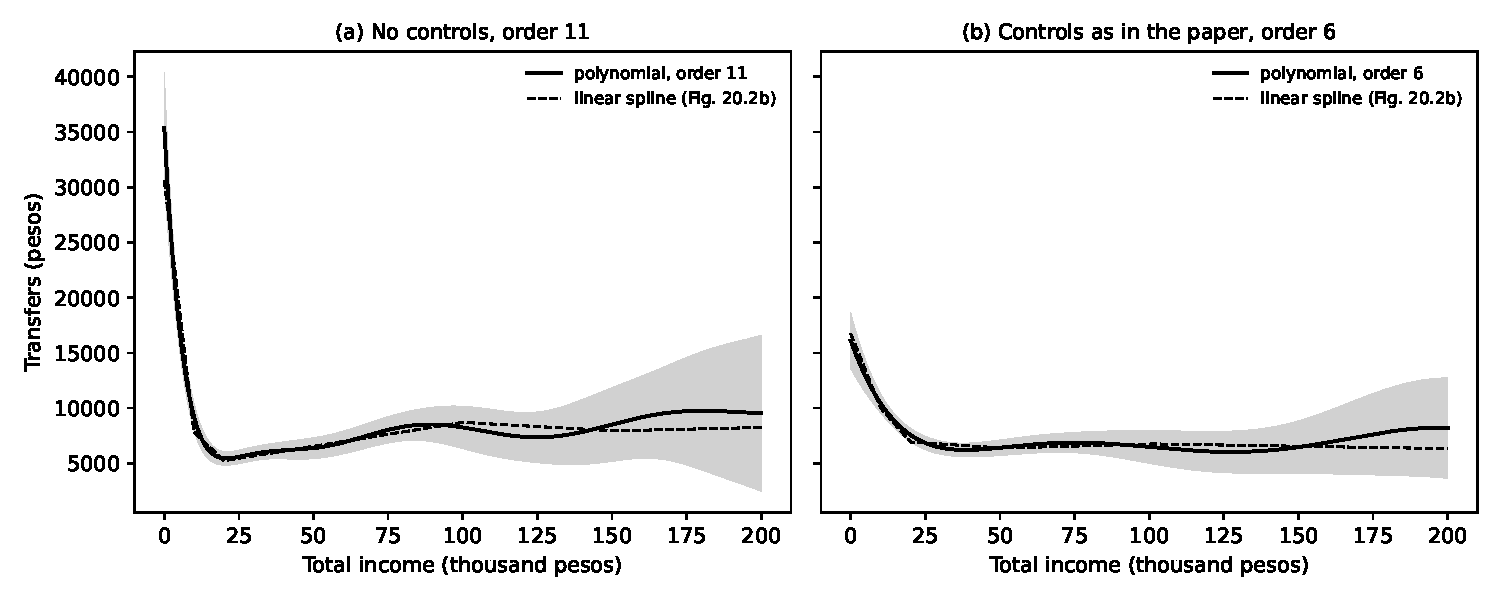
\includegraphics[width=\textwidth]{figures/ch20_17.pdf}
\end{center}
Estimated transfers (s.e.) with the paper's controls, at the mean of the controls: $16{,}106\ (1290)$ at zero income, $10{,}443\ (444)$
at $10{,}000$, $7578\ (309)$ at $20{,}000$, $6428\ (310)$ at $30{,}000$, $6411\ (361)$ at $50{,}000$, $6485\ (757)$ at $100{,}000$ and $6467\ (1216)$ at $150{,}000$ pesos.

\emph{Comparison with Figure 20.2(b).}  With controls, the polynomial closely tracks the book's linear spline
(dashed).  Transfers fall steeply at low incomes, with average slopes of $-0.57$ between 0 and $10{,}000$ pesos and $-0.29$
between $10{,}000$ and $20{,}000$ (the spline gives $-0.7$ and $-0.3$).  They are then essentially flat from about $25{,}000$ pesos
onward.  This is the crowding-out pattern predicted by altruistic transfer models, though with a
slope smaller than the theoretical $-1$.  The polynomial is smoother around the knots and its bands widen
at high incomes, where data are sparse.  Without controls the initial decline is much steeper (average slope
$-2.6$ below $10{,}000$ pesos): part of what looks like crowding out is explained by household characteristics
(education, employment status, household composition) that are correlated with very low income.  The
estimate above $150{,}000$ pesos is imprecise in all specifications.
\end{ex}

%%---------------------------------------------------------------------------
\begin{ex}{20.18}
Same specification as Table 20.1: cubics in $c=\text{classize}/40$ and $d=\text{disadvantaged}/14$, the interaction $cd$, enrollment and a
grade-4 dummy.  Instruments are $p/40$, $(p/40)^{2}$, $(p/40)^{3}$ and $(p/40)d$, where $p$ is the Maimonides prediction
$p=\text{enrollment}/(1+\lfloor(\text{enrollment}-1)/40\rfloor)$.  Standard errors are clustered by school.

(Two book typos.  (20.42) should read $1+\lfloor(\text{enrollment}-1)/40\rfloor$ in the denominator, as in the book's own code.  In the
class-size effect $\theta=\frac12\beta_1+\frac34\beta_2+\frac78\beta_3+\frac12\beta_7\ol d$, the last term involves the interaction coefficient $\beta_7$, not $\beta_4$.  With $\ol d\approx1$
this reproduces $\wh\theta=-2.96\ (1.21)$ for reading.)
\begin{center}
\small
\begin{tabular}{lcc}
\toprule
 & reading (Table 20.1) & math\\
\midrule
$c$, $c^{2}$, $c^{3}$ & $34.2$, $-61.2$, $29.0$ & $22.7$, $-28.1$, $10.0$\\
 & $(33.5)$, $(53.0)$, $(26.9)$ & $(45.0)$, $(71.7)$, $(36.6)$\\
$cd$ & $0.81$ $(1.77)$ & $-2.68$ $(2.24)$\\
$d$, $d^{2}$, $d^{3}$ & $-12.4$, $3.33$, $-0.377$ & $-7.95$, $2.90$, $-0.387$\\
 & $(1.7)$, $(0.54)$, $(0.078)$ & $(2.17)$, $(0.70)$, $(0.098)$\\
enrollment & $0.015$ $(0.007)$ & $0.030$ $(0.008)$\\
grade 4 & $-1.96$ $(0.16)$ & $1.53$ $(0.22)$\\
\midrule
Wald, no class-size effect ($\chi^{2}_4$) & $12.7$ ($p=0.013$) & $3.1$ ($p=0.54$)\\
$\theta$: class size $20\to40$ & $-2.96$ $(1.21)$ & $-2.27$ $(1.58)$\\
\bottomrule
\end{tabular}
\end{center}
\begin{center}
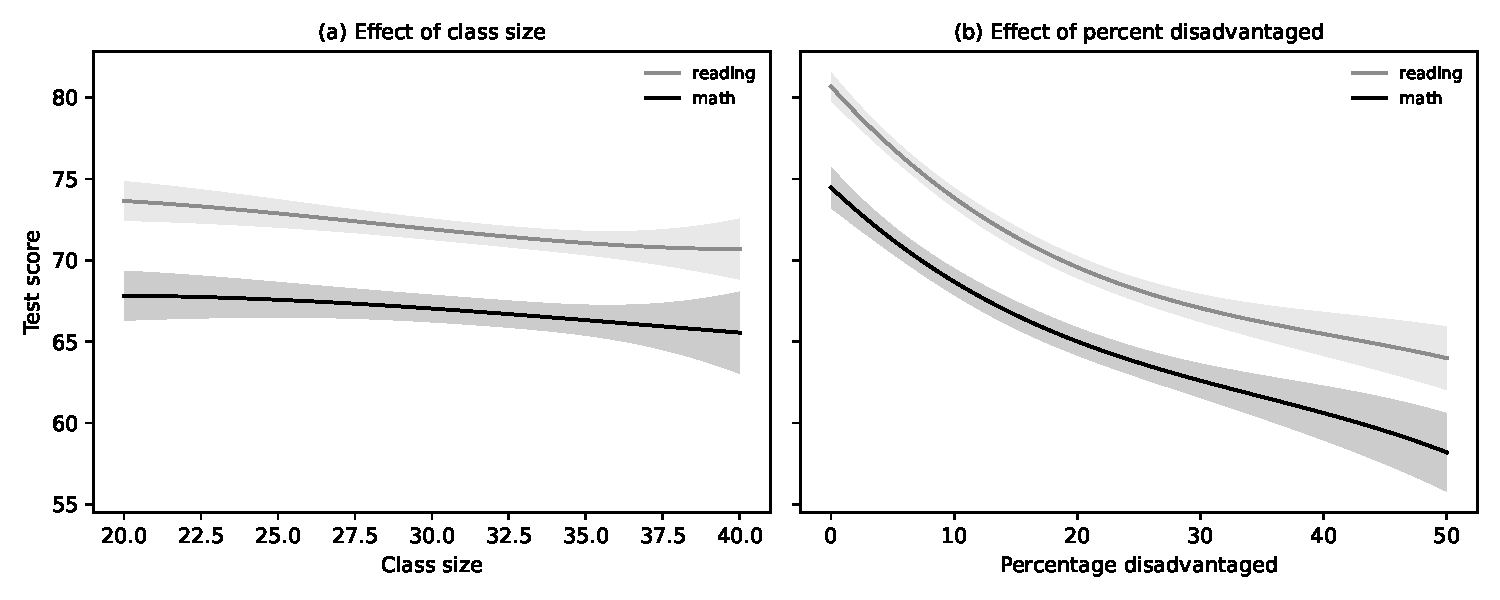
\includegraphics[width=\textwidth]{figures/ch20_18.pdf}
\end{center}
\emph{Comparison.}  The estimated class-size effect on math is similar in magnitude to that on reading, a
decline of about $2.3$ points as class size rises from 20 to 40, again nearly linear.  But it is estimated less
precisely and is not statistically significant: the Wald test of no class-size effect has $p=0.54$, and $\wh\theta$ has
$t=-1.4$.  The effect of the share of disadvantaged students is again large, nonlinear and precisely
estimated: math scores fall from $74.5$ at 0\% to $65.0$ at 20\% and $58.2$ at 50\% disadvantaged, a decline of about 16 points,
similar to that for reading.  Fourth graders score higher than fifth graders in math but lower in reading;
since the tests differ by grade, such level differences are not comparable.  Overall, the nonparametric IV evidence for a class-size effect is
substantially weaker for math than for reading.
\end{ex}

%% ===========================================================================
%% Chapter 21. Regression Discontinuity
%% ===========================================================================
\solchapter{21}{Regression Discontinuity}

\begin{center}
\begin{minipage}{0.86\textwidth}
\small
Solutions to all 9 exercises of Chapter 21 of Bruce E.\ Hansen, \emph{Econometrics}
(Princeton University Press, 2022).  Exercises 21.5--21.9 use \texttt{LM2007} (Ludwig and Miller's Head Start data, 2783
counties, cut-off $c=59.1984$).  Local linear RDD estimates use the normalized Triangular kernel
$K(u)=(1-|u|/\sqrt6)\indic\{|u|<\sqrt6\}/\sqrt6$, estimated separately on each side of the cut-off.  Standard errors follow Section 21.5,
using leave-one-out prediction errors.  The baseline estimate of Table 21.1, $-1.51\ (0.71)$, is reproduced exactly.
\end{minipage}
\end{center}

\bigskip
\hrule
\bigskip

Notation: $m(x)=\E[Y\given X=x]$, $m_d(x)=\E[Y_d\given X=x]$, $m(c\pm)$ the one-sided limits, and $\theta(x)=m_1(x)-m_0(x)$.

%%---------------------------------------------------------------------------
\begin{ex}{21.1}
Now $m(x)=m_1(x)\indic\{x\le c\}+m_0(x)\indic\{x>c\}$.  Under continuity of $m_0$ and $m_1$ at $c$,
\[
  \theta=\theta(c)=m_1(c)-m_0(c)=m(c-)-m(c+).
\]
Only the sign convention changes: the treated side is now the left side, so $\wh\theta=\wh m(c-)-\wh m(c+)$.  Estimation is
otherwise identical (separate local linear fits on each side, the same bandwidth choices and standard
errors).  In regression form (21.4) define $D=\indic\{X\le c\}$ and the interaction $(X-c)D$; then $\wh\theta$ is again the coefficient
on $D$.  Whether the point $X=c$ is assigned to the treated or untreated side is immaterial for a continuous
running variable.
\end{ex}

%%---------------------------------------------------------------------------
\begin{ex}{21.2}
There are two discontinuities.  If $m_0$ and $m_1$ are continuous at $c_1$ and at $c_2$,
\[
  \theta(c_1)=m(c_1+)-m(c_1-),\qquad \theta(c_2)=m(c_2-)-m(c_2+).
\]
At $c_1$ units switch from untreated to treated, and at $c_2$ from treated to untreated.  So the conditional ATEs
at the two cut-offs are identified, and can be estimated by one-sided local linear regressions at each
boundary.  The hypothesis $\theta(c_1)=\theta(c_2)$ can be tested.  Nothing more is identified without extrapolation:
inside $(c_1,c_2)$ only $m_1$ is observed and outside only $m_0$, so $\theta(x)$ for other $x$ requires assumptions about the
unobserved potential-outcome functions.
\end{ex}

%%---------------------------------------------------------------------------
\begin{ex}{21.3}
The observed outcome is $Y=Y_0\indic\{X<c\}+Y_1\indic\{X\ge c\}$.  The indicators are functions of $X$, so conditional on $X=x$ they are
constants and can be taken outside the expectation:
\begin{align*}
  m(x)=\E[Y\given X=x]&=\indic\{x<c\}\E[Y_0\given X=x]+\indic\{x\ge c\}\E[Y_1\given X=x]\\
  &=m_0(x)\indic\{x<c\}+m_1(x)\indic\{x\ge c\}.
\end{align*}
\end{ex}

%%---------------------------------------------------------------------------
\begin{ex}{21.4}
The regressors of (21.4), $(1,\ X,\ (X-c)D,\ D)$, span the same space as $\bigl((1-D),\ (1-D)(X-c),\ D,\ D(X-c)\bigr)$: a separate intercept and slope
on each side of the cut-off, expressed in deviations from $c$.  A regression on this reparameterization
decouples, so the fit is the same as two separate least squares regressions of $Y$ on $(1,X-c)$: one on
$c-h\le X<c$ and one on $c\le X\le c+h$.  In the original parameterization the left intercept at $c$ is $\beta_0+\beta_1c$ and the
right intercept is $\beta_0+\beta_1c+\theta$.  Hence
\[
  \wh\theta=\wh m(c+)-\wh m(c-).
\]
An unweighted least squares fit of $(1,X-c)$ on the observations with $|X-c|\le h$ is exactly the local linear estimator at the
boundary point $x=c$ with the (unnormalized) Rectangular kernel $K(u)=\frac12\indic\{|u|\le1\}$ and bandwidth $h$, computed from
one side.  So (21.4) is the RDD local linear estimator (21.2) with that kernel.  The normalized (unit-variance)
Rectangular kernel has support $[-\sqrt3,\sqrt3]$, so a normalized bandwidth $h$ corresponds to the window $\pm h\sqrt3$.  One
caveat: the conventional (homoskedastic) regression standard errors from (21.4) impose a common error
variance on both sides.  Heteroskedasticity-robust standard errors coincide with those of the two separate
regressions.
\end{ex}

%%---------------------------------------------------------------------------
\begin{ex}{21.5}
Least squares on the window, White (HC0) standard errors as in the book's code:
\begin{center}
\begin{tabular}{lccccc}
\toprule
window & $n$ & $\wh\beta_0$ & $\wh\beta_1$ & $\wh\beta_3$ & $\wh\theta$\\
\midrule
$c\pm7$    & $427$  & $-4.13$ $(10.69)$ & $0.130$ $(0.196)$ & $0.004$ $(0.227)$ & $-1.86$ $(1.06)$\\
$c\pm8$    & $482$  & $-3.11$ $(9.13)$ & $0.111$ $(0.168)$ & $0.181$ $(0.235)$ & $-2.20$ $(1.06)$\\
$c\pm13.8$ & $751$  & $-1.01$ $(3.32)$ & $0.074$ $(0.066)$ & $0.044$ $(0.100)$ & $-1.57$ $(0.74)$\\
$c\pm20$   & $1059$ & $-0.01$ $(2.02)$ & $0.056$ $(0.041)$ & $0.009$ $(0.061)$ & $-1.30$ $(0.61)$\\
\bottomrule
\end{tabular}
\end{center}
\rmk{Book discrepancy.  The text says (21.5) uses the window $59.1984\pm13.8$ with $482$ observations.  But the reported estimates,
$-3.11\ (9.13)$, $0.11\ (0.17)$, $0.18\ (0.23)$, $-2.20\ (1.06)$, and the sample size $482$ are exactly those of the window $\pm8$ (row 2).  The window
$\pm13.8$ contains $751$ counties and gives $\wh\theta=-1.57\ (0.74)$, very close to the Triangular-kernel estimate of Table 21.1.  (The book's
R code computes $h_0=h\sqrt3$ but then selects the sample with $h$.)}

The estimated effect is negative for every window: grant-writing assistance lowered Head Start-related
mortality among 5--9 year olds by $1.3$--$2.2$ deaths per 100,000.  Narrower windows give larger effects and larger
standard errors: with $\pm7$ the effect is significant only at 10\% ($p=0.08$), while with $\pm13.8$ and $\pm20$, $p=0.03$.
\end{ex}

%%---------------------------------------------------------------------------
\begin{ex}{21.6}
\begin{center}
\begin{tabular}{lcccc}
\toprule
$h$ (normalized) & $h$ ($[-1,1]$ Triangular) & $\wh\theta$ & s.e. & p-value\\
\midrule
4  & 9.8  & $-2.10$ & $(1.02)$ & $0.038$\\
8  & 19.6 & $-1.51$ & $(0.71)$ & $0.035$\\
12 & 29.4 & $-1.25$ & $(0.58)$ & $0.030$\\
\bottomrule
\end{tabular}
\end{center}
The baseline $-1.51\ (0.71)$ reproduces Table 21.1.  The estimated untreated mortality at the cut-off is $\wh m(c-)=3.31$, so the
effect is a reduction of about 45\%.  Halving the bandwidth raises the estimated effect to $-2.1$ and inflates
the standard error by about 40\%.  Increasing it to 12 shrinks both.  This is the expected bias--variance pattern
(Section 21.6): larger bandwidths straighten the fitted curves, and in particular the curvature above the
cut-off, attenuating the jump.  All three estimates are significant at 5\%.
\end{ex}

%%---------------------------------------------------------------------------
\begin{ex}{21.7}
Injuries are not a target of Head Start's health services, so no discontinuity is expected.
\begin{center}
\begin{tabular}{lccc}
\toprule
$h$ & 4 & 8 & 12\\
\midrule
$\wh\theta$ (s.e.) & $0.25$ $(3.32)$ & $1.62$ $(2.58)$ & $1.17$ $(2.31)$\\
\bottomrule
\end{tabular}
\end{center}
(Simple regression, window $\pm13.8$: $2.42\ (2.71)$.)  Relative to a baseline injury mortality of about $23$ per 100,000 at the cut-off,
the estimates are small, positive and far from significant at every bandwidth.  There is no discontinuity
in non-targeted child mortality.  This supports the interpretation that the Head Start-related estimate
reflects the program rather than a general discontinuity in child health or data quality at the cut-off.
\end{ex}

%%---------------------------------------------------------------------------
\begin{ex}{21.8}
\begin{center}
\begin{tabular}{lccc}
\toprule
$h$ & 4 & 8 & 12\\
\midrule
$\wh\theta$ (s.e.) & $2.33$ $(5.89)$ & $4.48$ $(4.35)$ & $6.34$ $(3.84)$\\
\bottomrule
\end{tabular}
\end{center}
(Simple regression, $\pm13.8$: $4.57\ (4.57)$.)  Adults were not exposed to Head Start, so their mortality from the same causes is a
natural placebo.  The estimates are positive, not negative, and insignificant ($p=0.30$ at $h=8$; $p=0.10$ at $h=12$).  They are
tiny relative to the adult rate of about $132$ per 100,000 (3\%).  There is no evidence of a mortality
reduction among adults, as expected if the child effect is due to Head Start.
\end{ex}

%%---------------------------------------------------------------------------
\begin{ex}{21.9}
\begin{center}
\begin{tabular}{lccc}
\toprule
$h$ & 4 & 8 & 12\\
\midrule
$\wh\theta$ (s.e.) & $-3.74$ $(1.74)$ & $-1.90$ $(1.66)$ & $-1.17$ $(1.52)$\\
p-value & $0.032$ & $0.25$ & $0.44$\\
\bottomrule
\end{tabular}
\end{center}
(Simple regression, $\pm13.8$: $-1.58\ (1.83)$.)  Before the program existed there should be no discontinuity.  At the baseline bandwidth
$h=8$ the estimate is insignificant, as are those at $h=12$ and in the simple regression.  This is the evidence
Ludwig and Miller use to argue that the post-program jump is causal.  Two cautions are in order, however.
The point estimates are negative and, in absolute terms, as large as the post-program effect.  At the
small bandwidth $h=4$ the pre-period estimate is significant ($p=0.03$).  Relative to the much higher 1959--64 mortality
rate ($\approx9.8$ per 100,000 at the cut-off versus $3.3$ in 1973--83) the pre-period jump is proportionally smaller (about 20\% versus
45\%).  But the placebo test is not sharp enough to rule out a pre-existing discontinuity.  The post-program
estimate should therefore be viewed as suggestive rather than conclusive.  A difference-in-discontinuities
comparison (post minus pre) would be a natural next step.
\end{ex}

\medskip
\noindent\textbf{Figure.}  Local linear RDD fits with 95\% pointwise bands ($h=8$) for the four outcomes of Exercises 21.6--21.9.
\begin{center}
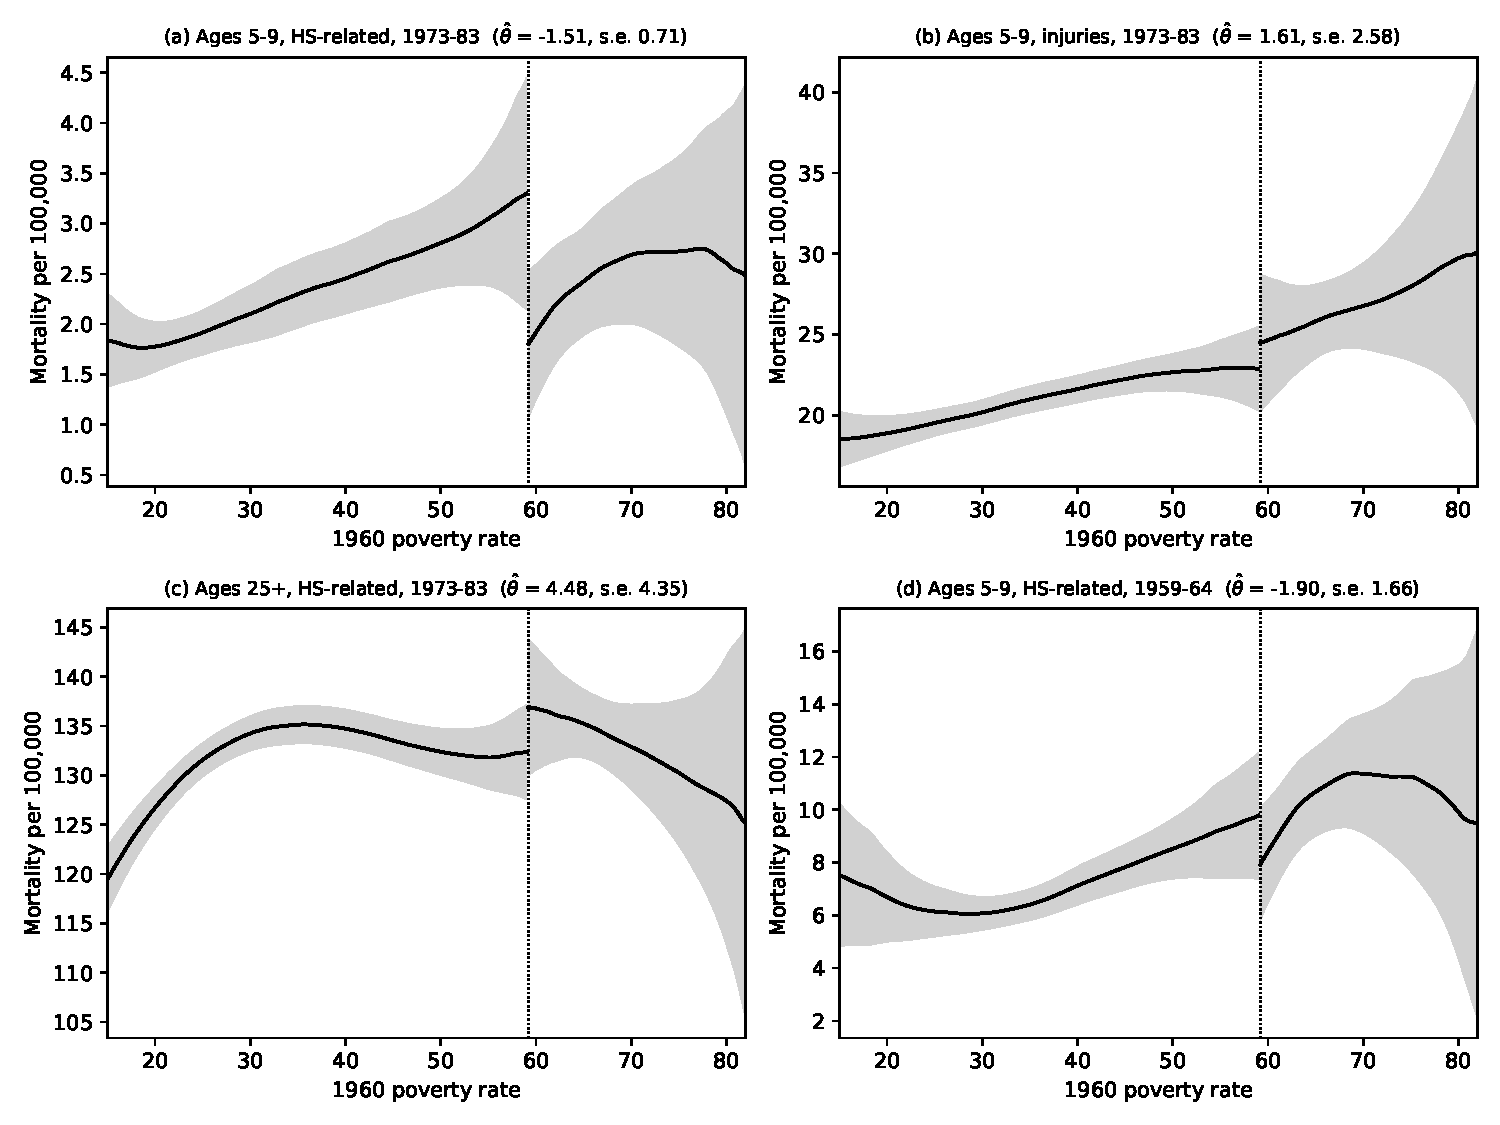
\includegraphics[width=\textwidth]{figures/ch21_rdd.pdf}
\end{center}

%% ===========================================================================
%% Chapter 22. M-Estimators
%% ===========================================================================
\solchapter{22}{M-Estimators}

\begin{center}
\begin{minipage}{0.86\textwidth}
\small
Solutions to all 4 exercises of Chapter 22 of Bruce E.\ Hansen, \emph{Econometrics}
(Princeton University Press, 2022).  All asymptotic covariance matrices follow Theorem 22.4: $\sqrt n(\wh\theta-\theta_0)\convd N(0,V)$ with
$V=Q^{-1}\Omega Q^{-1}$, $Q=\E\bigl[\partial^{2}\rho/\partial\theta\partial\theta'\bigr]$ and $\Omega=\E[\psi\psi']$.
\end{minipage}
\end{center}

\bigskip
\hrule
\bigskip

Notation: $e=Y-X'\theta_0$.  For Exercises 22.2--22.4 we give $V$ in general and also in the leading special case where $e$ is
independent of $X$, which lets the expectations factor.

%%---------------------------------------------------------------------------
\begin{ex}{22.1}
\textbf{(a)}  By independence, $\Pc{Y\le y}{X=x}=\Pc{e\le y-x'\theta}{X=x}=F(y-x'\theta)$, where $F$ is the distribution function of $e$.
Differentiating in $y$ gives the conditional density $f(y-x'\theta)$.

\textbf{(b)}  The MLE is the m-estimator with the negative log-density:
\[
  \rho(Y,X,\theta)=-\log f(Y-X'\theta),\qquad \psi(Y,X,\theta)=\frac{\partial\rho}{\partial\theta}=X\,\frac{f'(Y-X'\theta)}{f(Y-X'\theta)}=-X\,\phi(Y-X'\theta),
\]
where $\phi(u)=-f'(u)/f(u)$ is the location score of $f$.

\textbf{(c)}  At $\theta_0$, $\psi_i=-X_i\phi(e_i)$, and $\E[\phi(e)]=\int f'(u)\,du=0$, so the scores have mean zero.  With $\mathcal I_f=\E[\phi(e)^{2}]=\int(f')^{2}/f$ (the Fisher
information for location) and independence,
\[
  \Omega=\E[XX'\phi(e)^{2}]=\E[XX']\,\mathcal I_f .
\]
For the Hessian, $S(\theta)=\E[-\log f(e-X'(\theta-\theta_0))]$, so $Q=\E[XX']\,\E[\phi'(e)]$ when $f$ is twice differentiable.  Integrating by parts,
\[
  \E[\phi'(e)]=\int\Bigl(\frac{f'(u)^{2}}{f(u)}-f''(u)\Bigr)du=\mathcal I_f
\]
(the boundary terms vanish under the usual regularity conditions).  The same limit holds with only one
derivative, by differentiating $\E[X\phi(e-X'\delta)]$ under the integral.  So $Q=\Omega$, the information matrix equality, and
\[
  V=Q^{-1}=\bigl(\E[XX']\bigr)^{-1}\frac{1}{\mathcal I_f}.
\]
For normal errors $\mathcal I_f=1/\sigma^{2}$ and $V=\sigma^{2}\E[XX']^{-1}$, the OLS variance.  For other densities $\mathcal I_f>1/\var[e]$ (Cram\'er--Rao), so the MLE
improves on OLS.  For example, Laplace errors with scale $b$ have $\mathcal I_f=1/b^{2}=2/\var[e]$, halving the variance.
\end{ex}

%%---------------------------------------------------------------------------
\begin{ex}{22.2}
\textbf{(a)}  $\rho(Y,X,\theta)=g(Y-X'\theta)$ and, for differentiable $g$, $\psi(Y,X,\theta)=-X\,g'(Y-X'\theta)$.

\textbf{(b)}  The estimand $\theta_0$ is defined by the population first-order condition $\E[X\,g'(Y-X'\theta_0)]=0$.  This equals the regression
coefficient only if $\E[g'(e)\given X]=0$, e.g.\ when $e$ is symmetric about zero given $X$ and $g$ is even.  With $e=Y-X'\theta_0$ and $g$ twice
differentiable,
\[
  Q=\E\bigl[XX'g''(e)\bigr],\qquad \Omega=\E\bigl[XX'g'(e)^{2}\bigr],\qquad V=Q^{-1}\Omega Q^{-1}.
\]
If $e$ is independent of $X$,
\[
  V=\bigl(\E[XX']\bigr)^{-1}\frac{\E[g'(e)^{2}]}{\bigl(\E[g''(e)]\bigr)^{2}} .
\]
(If $g$ is not twice differentiable, as for LAD, $Q$ is computed as $\partial^{2}S(\theta)/\partial\theta\partial\theta'$ at $\theta_0$; see Section 22.7.)  Least squares,
$g(u)=u^{2}/2$, gives $\E[g'^{2}]/(\E g'')^{2}=\sigma^{2}$, as it should.
\end{ex}

%%---------------------------------------------------------------------------
\begin{ex}{22.3}
\textbf{(a)}  $g$ is a flat-bottomed, strictly convex, even function (left panel below).  It is a polynomial, so it is continuous
and infinitely differentiable: $g'(u)=u^{3}$ and $g''(u)=3u^{2}$.  Compared with least squares it penalizes small residuals less
and large residuals much more.
\begin{center}
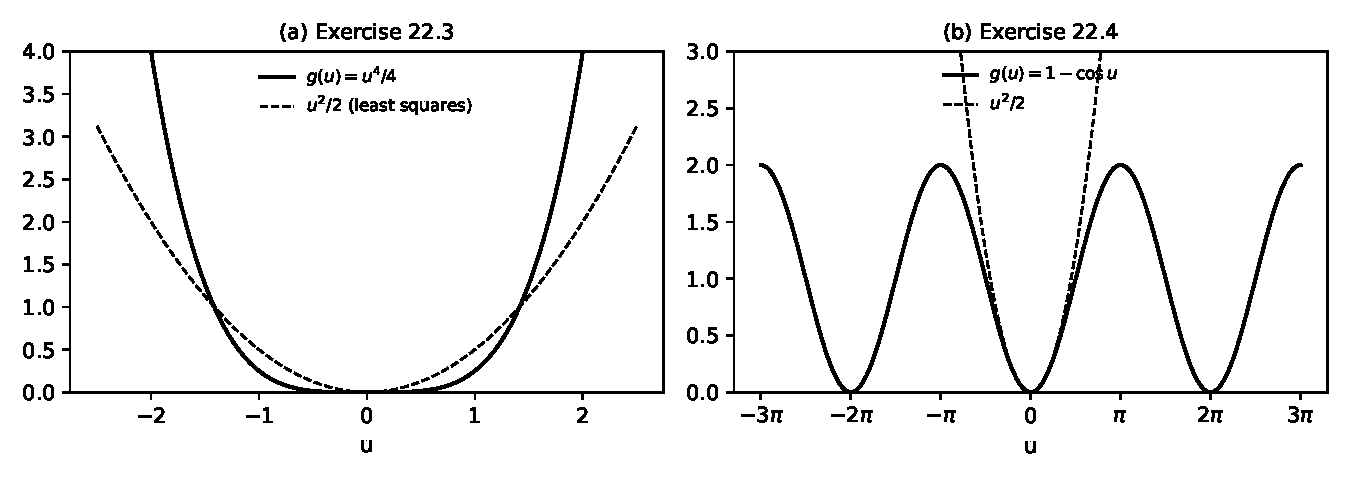
\includegraphics[width=0.95\textwidth]{figures/ch22_g.pdf}
\end{center}
\textbf{(b)}  $\rho(Y,X,\theta)=\frac14(Y-X'\theta)^{4}$ and $\psi(Y,X,\theta)=-X(Y-X'\theta)^{3}$.

\textbf{(c)}  With $e=Y-X'\theta_0$, where $\theta_0$ solves $\E[Xe^{3}]=0$,
\[
  Q=3\,\E[XX'e^{2}],\qquad \Omega=\E[XX'e^{6}],\qquad V=\tfrac19\bigl(\E[XX'e^{2}]\bigr)^{-1}\E[XX'e^{6}]\bigl(\E[XX'e^{2}]\bigr)^{-1},
\]
which requires $\E\|X\|^{2}e^{6}<\infty$.  Under independence, $V=\E[XX']^{-1}\,\E[e^{6}]/\bigl(9\sigma^{4}\bigr)$ with $\sigma^{2}=\E[e^{2}]$.  For normal errors $\E[e^{6}]=15\sigma^{6}$, so $V=\frac53\sigma^{2}\E[XX']^{-1}$,
67\% larger than OLS.  For light-tailed (platykurtic) errors it can beat OLS.  For uniform errors on $[-a,a]$,
$\E e^{6}/(9\sigma^{4})=(a^{6}/7)/(9a^{4}/9)=a^{2}/7$ versus $\sigma^{2}=a^{2}/3$, so the fourth-power estimator is more than twice as
efficient as OLS.  The criterion is strictly convex, so the minimizer is unique and easy to compute.
\end{ex}

%%---------------------------------------------------------------------------
\begin{ex}{22.4}
\textbf{(a)}  $g$ is even, bounded between 0 and 2, and periodic with period $2\pi$.  It behaves like $u^{2}/2$ near zero but levels off, so
it is not convex (right panel above).  It is continuous and infinitely differentiable: $g'(u)=\sin u$, $g''(u)=\cos u$.

\textbf{(b)}  $\rho(Y,X,\theta)=1-\cos(Y-X'\theta)$ and $\psi(Y,X,\theta)=-X\sin(Y-X'\theta)$.

\textbf{(c)}  With $\theta_0$ solving $\E[X\sin(Y-X'\theta_0)]=0$,
\[
  Q=\E\bigl[XX'\cos(e)\bigr],\qquad \Omega=\E\bigl[XX'\sin^{2}(e)\bigr],\qquad V=Q^{-1}\Omega Q^{-1},
\]
and under independence $V=\E[XX']^{-1}\,\E[\sin^{2}e]/(\E[\cos e])^{2}$.  Theorem 22.4 requires $Q>0$, i.e.\ $\E[\cos e]>0$: the errors must be concentrated
well within $(-\pi/2,\pi/2)$ relative to the period.  For $e\sim N(0,\sigma^{2})$, $\E\cos e=e^{-\sigma^{2}/2}$ and $\E\sin^{2}e=(1-e^{-2\sigma^{2}})/2$, so
\[
  V=\E[XX']^{-1}\sinh(\sigma^{2})\approx\sigma^{2}\E[XX']^{-1}\quad\text{for small }\sigma^{2},
\]
nearly efficient for small errors but rapidly worse as $\sigma$ grows.

\emph{Remarks.}  Because $\psi$ is bounded ($|\sin|\le1$) and redescending, the estimator is robust to outliers, like Andrews' sine
estimator.  But periodicity creates identification problems.  If $X$ contains an intercept, the criterion is unchanged
when the intercept is shifted by $2\pi$, so $\theta$ is identified only up to that shift.  More generally $S(\theta)$ has multiple
local minima, so a restricted parameter space and good starting values (e.g.\ OLS) are needed.  The data
should be scaled so that the residuals are small relative to $\pi$.
\end{ex}

%% ===========================================================================
%% Chapter 23. Nonlinear Least Squares
%% ===========================================================================
\solchapter{23}{Nonlinear Least Squares}

\begin{center}
\begin{minipage}{0.86\textwidth}
\small
Solutions to all 10 exercises of Chapter 23 of Bruce E.\ Hansen, \emph{Econometrics}
(Princeton University Press, 2022).  Exercises 23.8--23.10 use \texttt{PSS2017}, \texttt{RR2010} and \texttt{Nerlove1963}.  As a check, the
CES and regression-kink estimates of Table 23.1 are reproduced to the reported precision.  Standard errors
use (23.6) with the NLLS gradient $\wh m_{\theta i}$ as the effective regressor: heteroskedasticity-robust, or clustered by country
for the CES model.
\end{minipage}
\end{center}

\bigskip
\hrule
\bigskip

%%---------------------------------------------------------------------------
\begin{ex}{23.1}
\textbf{(a)}  The CEF is the constant $\exp(\theta)$, which is nonlinear in $\theta$, so formally this is a nonlinear regression model.  But it is
nonlinear only because of the parameterization: with $\mu=\exp(\theta)$ it becomes the linear intercept-only model $Y=\mu+e$.

\textbf{(b)}  Yes.  Estimate $\mu$ by least squares, $\wh\mu=\ol Y$, and set $\wh\theta=\log\ol Y$ (defined when $\ol Y>0$).

\textbf{(c)}  It is the same.  NLLS minimizes $\sum(Y_i-e^{\theta})^{2}$, and the first-order condition $-2e^{\theta}\sum(Y_i-e^{\theta})=0$ gives $e^{\wh\theta}=\ol Y$.  Least squares is
invariant to one-to-one reparameterization.  If $\ol Y\le0$ the NLLS criterion has no minimizer (it decreases as $\theta\to-\infty$),
matching the fact that $\log\ol Y$ is undefined.
\end{ex}

%%---------------------------------------------------------------------------
\begin{ex}{23.2}
No, not in the sense of this chapter, although it looks like one.  A nonlinear regression model has the
form $Y=m(X,\theta)+e$ with $\E[e\given X]=0$ for a fixed dependent variable.  Here the dependent variable itself depends on the
parameter $\lambda$, and the model restricts $\E[Y^{(\lambda)}\given X]$, not $\E[Y\given X]$.  The implied CEF of $Y$,
\[
  \E[Y\given X]=\E\bigl[\bigl(1+\lambda(\beta_0+\beta_1X+e)\bigr)^{1/\lambda}\given X\bigr],
\]
depends on the whole conditional distribution of $e$, not just on $(\lambda,\beta_0,\beta_1)$.  Consequently NLLS on $\sum(Y_i^{(\lambda)}-\beta_0-\beta_1X_i)^{2}$
is not valid.  The criterion is not comparable across $\lambda$, because the scale of $Y^{(\lambda)}$ changes with $\lambda$, and minimizing it
over $\lambda$ can simply shrink the dependent variable.  The model is a transformation model.  It is estimated by
maximum likelihood (e.g.\ under normal $e$), whose log-likelihood includes the Jacobian term $(\lambda-1)\sum\log Y_i$.  Equivalently, one
can use least squares on $Y^{(\lambda)}$ divided by $\dot Y^{\lambda-1}$ with $\dot Y$ the geometric mean.
\end{ex}

%%---------------------------------------------------------------------------
\begin{ex}{23.3}
\textbf{(a)}  No.  For any $k\ne0$, $(k\beta_1,k\beta_2,k\beta_3)$ gives the same regression function, so the parameters are identified only up to
scale.

\textbf{(b)}  The ratios are identified (provided $\beta_1\ne0$, $\beta_3\ne0$, and $X$ takes at least two values).  Normalize $\beta_1=1$ and write
\[
  Y=\frac{1}{\gamma_1+\gamma_2X}+e,\qquad \gamma_1=\beta_2/\beta_1,\quad \gamma_2=\beta_3/\beta_1,
\]
and estimate $(\gamma_1,\gamma_2)$ by NLLS with robust standard errors.  Equivalent normalizations are possible, e.g.\ $\beta_2=1$ giving
$Y=\delta_1/(1+\delta_2X)$ with $\delta_1=\beta_1/\beta_2$, $\delta_2=\beta_3/\beta_2$.  If $\beta_1=0$ the regression function is identically zero and neither ratio is
identified.
\end{ex}

%%---------------------------------------------------------------------------
\begin{ex}{23.4}
\textbf{(a)}  Yes, provided $\beta_1\ne0$ and $X$ is non-degenerate.  If $m(x)=\beta_1e^{\beta_2x}=b_1e^{b_2x}$ at two values $x_1\ne x_2$, dividing gives
$e^{\beta_2(x_1-x_2)}=e^{b_2(x_1-x_2)}$, so $b_2=\beta_2$ and then $b_1=\beta_1$.  If $\beta_1=0$, $\beta_2$ is not identified; if $X$ is constant, only $\beta_1e^{\beta_2X}$ is.

\textbf{(b)}  The linearized regressor is $m_\theta(X,\theta)=\bigl(e^{\beta_2X},\ \beta_1Xe^{\beta_2X}\bigr)'$.  With $\wh m_{\theta i}=m_\theta(X_i,\wh\theta)$ and NLLS residuals $\wh e_i$,
\[
  \wh Q=\frac1n\sum_{i=1}^{n}\wh m_{\theta i}\wh m_{\theta i}',\qquad \wh\Omega=\frac1n\sum_{i=1}^{n}\wh m_{\theta i}\wh m_{\theta i}'\wh e_i^{2},\qquad \wh V_{\wh\theta}=\frac1n\wh Q^{-1}\wh\Omega\wh Q^{-1},
\]
with standard errors the square roots of the diagonal of $\wh V_{\wh\theta}$ (or $n^{-1}\wh Q^{-1}\wh\sigma^{2}$ under homoskedasticity).
\end{ex}

%%---------------------------------------------------------------------------
\begin{ex}{23.5}
The conditional log-likelihood is
\[
  \ell_n(\theta,\sigma^{2})=-\frac n2\log(2\pi\sigma^{2})-\frac1{2\sigma^{2}}\sum_{i=1}^{n}\bigl(Y_i-m(X_i,\theta)\bigr)^{2}.
\]
For any $\sigma^{2}$, maximizing over $\theta$ is equivalent to minimizing the sum of squared errors, so $\wh\theta_{\rm mle}=\wh\theta_{\rm nlls}$.  Concentrating,
$\partial\ell_n/\partial\sigma^{2}=0$ gives $\wh\sigma^{2}_{\rm mle}=n^{-1}\sum_i\bigl(Y_i-m(X_i,\wh\theta)\bigr)^{2}$, the average squared NLLS residual.
\end{ex}

%%---------------------------------------------------------------------------
\begin{ex}{23.6}
\textbf{(a)}  The order condition is $\ell\ge k$.  The local rank condition is that $G=\E\bigl[\partial g/\partial\theta'\bigr]=-\E\bigl[ZX'\exp(X'\theta_0)\bigr]$ has full column rank $k$.

\textbf{(b)}  The moment function is $g_i(\theta)=Z_i\bigl(Y_i-\exp(X_i'\theta)\bigr)$ with $\ol g_n(\theta)=n^{-1}\sum_ig_i(\theta)$.  The GMM estimator is
\[
  \wh\theta=\argmin_\theta\ \ol g_n(\theta)'\,\bs W\,\ol g_n(\theta),
\]
computed numerically.  A natural first step uses $\bs W=(n^{-1}\sum Z_iZ_i')^{-1}$ (nonlinear 2SLS).  With first-step residuals $\wt e_i$, the
efficient two-step estimator uses $\bs W=\wh\Omega^{-1}$, $\wh\Omega=n^{-1}\sum_iZ_iZ_i'\wt e_i^{2}$.  If $\ell=k$ it simply solves $\ol g_n(\theta)=0$.

\textbf{(c)}  Let $\wh G=-n^{-1}\sum_iZ_iX_i'\exp(X_i'\wh\theta)$ and $\wh\Omega=n^{-1}\sum_iZ_iZ_i'\wh e_i^{2}$ with $\wh e_i=Y_i-\exp(X_i'\wh\theta)$.  For efficient GMM $\wh V=(\wh G'\wh\Omega^{-1}\wh G)^{-1}$; for a
general weight matrix $\wh V=(\wh G'\bs W\wh G)^{-1}\wh G'\bs W\wh\Omega\bs W\wh G(\wh G'\bs W\wh G)^{-1}$.  Standard errors are the square roots of the diagonal of $n^{-1}\wh V$.
\end{ex}

%%---------------------------------------------------------------------------
\begin{ex}{23.7}
By the delta method $m(x,\wh\theta)$ is asymptotically normal, with variance equal to the quadratic form of the
gradient $m_\theta(x,\theta_0)$ in $\var[\wh\theta]$.  Hence
\[
  m(x,\wh\theta)\pm1.96\sqrt{m_\theta(x,\wh\theta)'\wh V\,m_\theta(x,\wh\theta)},\qquad m_\theta(x,\theta)=\frac{\partial}{\partial\theta}m(x,\theta),
\]
with the derivative computed analytically or numerically.  For strongly nonlinear $m$ the interval may be
improved by forming it on a transformed scale where $m$ is closer to linear and mapping back (e.g.\ on $\log m$
when $m>0$), or by a bootstrap.
\end{ex}

%%---------------------------------------------------------------------------
\begin{ex}{23.8}
The alternative inputs are available for $338$ country-years ($26$ countries).  They are measured in currency units
(around $10^{10}$), so we express them in billions.  This only shifts $\beta$ by $\nu\log10^{9}$ and helps the numerical
optimization.  NLLS uses a multi-start search.  Standard errors are clustered by country, with $\sigma=1/(1-\rho)$ by the delta method.
\begin{center}
\begin{tabular}{lcc}
\toprule
 & capacities (Table 23.1) & capital stocks\\
\midrule
$\rho$ & $0.36$ $(0.29)$ & $0.41$ $(0.25)$\\
$\nu$ & $1.05$ $(0.03)$ & $1.04$ $(0.03)$\\
$\alpha$ & $0.39$ $(0.06)$ & $0.32$ $(0.04)$\\
$\beta$ & $1.66$ $(0.30)$ & $9.02$ $(0.08)$ (inputs in billions)\\
$\sigma=1/(1-\rho)$ & $1.57$ $(0.71)$ & $1.70$ $(0.73)$\\
$n$ & $390$ & $338$\\
\bottomrule
\end{tabular}
\end{center}
The capacity column reproduces Table 23.1, except the standard error of $\sigma$.  The delta method gives
$s(\wh\sigma)=s(\wh\rho)/(1-\wh\rho)^{2}=0.288/0.405=0.71$.  The book's $0.46$ equals $s(\wh\rho)/(1-\wh\rho)$, which omits a factor $(1-\wh\rho)^{-1}$.

\emph{Comparison.}  The results are robust.  The substitution parameter is again positive ($\wh\rho=0.41$, $\wh\sigma=1.7$): clean and dirty
generation are substitutes, with an elasticity of substitution above one.  But the estimate is imprecise
($t=1.6$ for $\rho=0$), so Cobb--Douglas cannot be rejected.  The scale elasticity is essentially unchanged at $1.04$,
mildly increasing returns.  The main difference is the share parameter.  With capital stocks, clean capital
gets a smaller weight ($0.32$ versus $0.39$), more precisely estimated.  Dirty technology remains the dominant input.
\end{ex}

%%---------------------------------------------------------------------------
\begin{ex}{23.9}
Model: $\pi_t=\beta_1(D_{t-1}-c)_-+\beta_2(D_{t-1}-c)_++\beta_3\pi_{t-1}+\beta_4+e_t$, $n=218$.  We estimate it by concentrated least squares over $c$
(a fine grid between the 5\% and 95\% quantiles of debt, then local refinement), with robust standard
errors.  As a check, the same code with $Y$ = GDP growth reproduces Table 23.1: $0.033\ (0.025)$, $-0.067\ (0.047)$,
$0.28\ (0.09)$, $3.78\ (0.68)$, $c=43.9\ (11.9)$.
\[
  \wh\pi_t=-\underset{(0.116)}{0.108}(D_{t-1}-\underset{(9.5)}{15.8})_-+\underset{(0.018)}{0.041}(D_{t-1}-15.8)_++\underset{(0.095)}{0.458}\pi_{t-1}-\underset{(0.60)}{0.16}.
\]
\begin{center}
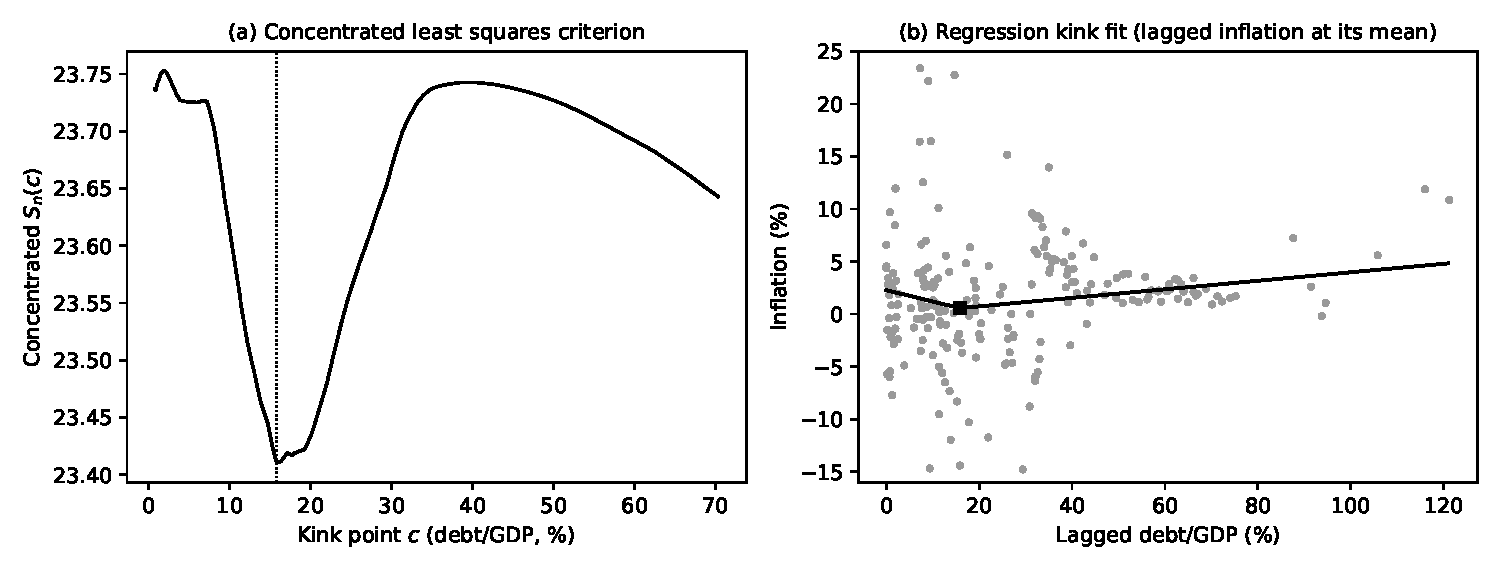
\includegraphics[width=\textwidth]{figures/ch23_09.pdf}
\end{center}
\emph{Interpretation.}  Below a debt ratio of about 16\% the slope is negative but insignificant.  Above it, inflation rises
with debt: each 10 points of debt/GDP are associated with $0.4$ points higher inflation in the next year,
significant at 5\%, plus the persistence captured by $\wh\beta_3=0.46$.  But the kink is poorly determined.  The concentrated
criterion (panel (a)) is very flat, and every $c$ between about 9\% and 70\% gives a sum of squared errors within 1\% of the
minimum.  The kink model reduces the sum of squared errors by only 1.4\% relative to a linear AR(1) with debt
(slope $0.019$).  Moreover, the standard error of $\wh c$ is not reliable because the regression kink estimator has a
non-standard distribution when the kink is weakly identified.  The evidence is consistent with a mild
positive association between high debt and subsequent inflation, most visible in war and post-war
episodes, rather than a well-defined threshold.
\end{ex}

%%---------------------------------------------------------------------------
\begin{ex}{23.10}
(The text's ``for values much above $\beta_7$'' should read ``much above $\gamma$''.)

\textbf{(a)}  $\log Q$ ranges from $0.69$ to $9.72$ ($n=145$).  Its 10th--15th smallest values are $3.09$--$3.76$ and its 10th--15th largest $8.67$--$8.97$.  We
restrict $\gamma\in[3.56,\ 8.72]$, the 13th smallest to the 13th largest observation, so that at least 13 firms lie on each side.

\textbf{(b)}  A multi-start local optimizer over all five parameters with $\gamma$ constrained to this range
($25\times5$ starting values) converges to a single minimum:
\[
  \wh\beta_1=-5.321,\quad \wh\beta_2=0.438,\quad \wh\beta_3=0.371,\quad \wh\beta_4=0.224,\quad \wh\gamma=6.875,\qquad \text{SSR}=14.272,
\]
against $22.114$ for the linear model.  If $\gamma$ is left unrestricted the global minimum ($\text{SSR}=12.94$) is at $\gamma=-0.78$, outside
the range of the data.  There the transition function is nearly constant except for the smallest firms, and the
fit relies on huge offsetting coefficients ($\wh\beta_2=16.3$, $\wh\beta_4=-15.4$).  This degenerate solution is exactly what
the restriction in (a) is designed to exclude.

\textbf{(c)}  Concentrating out the linear coefficients by OLS for each $\gamma$ on a grid of 4001 points gives the same estimates
($\wh\gamma=6.875$, SSR $14.272$).  The concentrated criterion has a single local minimum in the admissible range (panel (a)),
so the two methods agree.  Concentration is faster and more reliable, since it only requires a
one-dimensional search.
\begin{center}
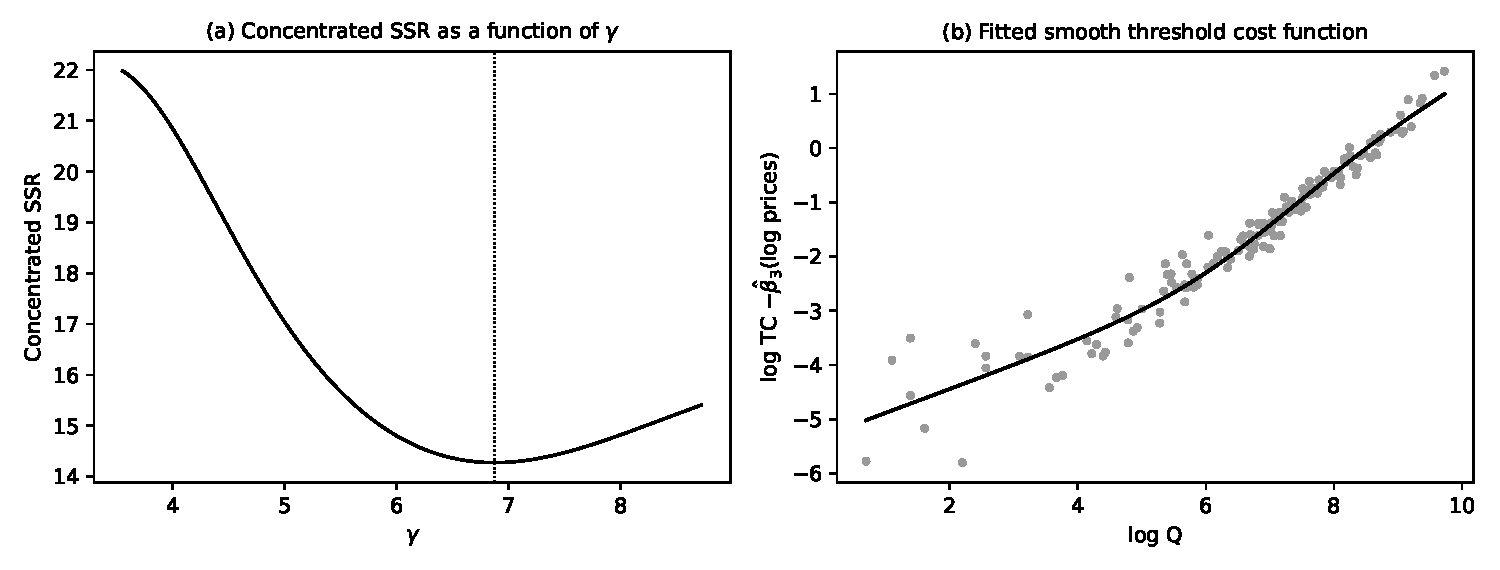
\includegraphics[width=\textwidth]{figures/ch23_10.pdf}
\end{center}
\textbf{(d)}  Heteroskedasticity-robust (homoskedastic) standard errors from (23.6):
\begin{gather*}
  \wh\beta_1=-5.32\ (0.49),\quad \wh\beta_2=0.438\ (0.100),\quad \wh\beta_3=0.371\ (0.044),\\
  \wh\beta_4=0.224\ (0.055),\quad \wh\gamma=6.88\ (0.36),
\end{gather*}
with homoskedastic values $0.60$, $0.048$, $0.062$, $0.029$ and $0.32$.  The cost elasticity with respect to output is $0.44$ for small
firms and $0.44+0.22=0.66$ for large firms.  The transition is centred at $\log Q=6.9$ (about $970$ million kWh), with $68$ firms
below and $77$ above.  Economies of scale are strong for small utilities (returns to scale $1/0.44\approx2.3$) and weaker,
though still present, for large ones ($1/0.66\approx1.5$).  This is the pattern Nerlove found by splitting the sample by
size, here captured by a smooth parametric transition.  The standard error of $\wh\gamma$ relies on smoothness of the
logistic transition; it would not be valid for a sharp threshold.
\end{ex}

%% ===========================================================================
%% Chapter 24. Quantile Regression
%% ===========================================================================
\solchapter{24}{Quantile Regression}

\begin{center}
\begin{minipage}{0.86\textwidth}
\small
Solutions to all 16 exercises of Chapter 24 of Bruce E.\ Hansen, \emph{Econometrics}
(Princeton University Press, 2022).  Quantile regressions are computed exactly by linear programming (the
Koenker--Bassett dual).  The code reproduces the tracking coefficients of Table 24.2 ($0.069$, $0.136$, $0.125$, $0.185$,
$0.151$).  Standard errors are nonparametric bootstrap standard errors (500 replications; 1000 clustered by school
for DDK), with 95\% bias-corrected (BC) percentile intervals as recommended in Section 24.8.
\end{minipage}
\end{center}

\bigskip
\hrule
\bigskip

Notation: $\rho_\tau(u)=u(\tau-\indic\{u<0\})$ is the check function, $\psi_\tau(u)=\tau-\indic\{u<0\}$, $F(\cdot\given x)$ is the conditional
distribution function of $Y$, and $q_\tau(x)$ is its $\tau$th quantile.

%%---------------------------------------------------------------------------
\begin{ex}{24.1}
Continuity implies $F(m(x)\given x)=\frac12$ and $\Pc{Y=m(x)}{X=x}=0$.  Hence
\begin{align*}
  \E[\sgn(e)\given X=x]&=\Pc{Y>m(x)}{X=x}-\Pc{Y<m(x)}{X=x}\\
  &=\bigl(1-F(m(x)\given x)\bigr)-F(m(x)\given x)=\tfrac12-\tfrac12=0.
\end{align*}
\end{ex}

%%---------------------------------------------------------------------------
\begin{ex}{24.2}
Fix $x$, write $m=m(x)$ and $F(\cdot)=F(\cdot\given x)$, and take $\theta>m$.  Pointwise,
\[
  |y-\theta|-|y-m|=\begin{cases}\theta-m, & y\le m,\\ \theta+m-2y\ \ge\ -(\theta-m), & m<y<\theta,\\ -(\theta-m), & y\ge\theta,\end{cases}
\]
so $|y-\theta|-|y-m|\ge(\theta-m)\bigl(\indic\{y\le m\}-\indic\{y>m\}\bigr)$.  Taking conditional expectations, which are finite since $\E|Y|<\infty$,
\[
  \E\bigl[|Y-\theta|-|Y-m|\given X=x\bigr]\ge(\theta-m)\bigl(F(m)-(1-F(m))\bigr)=(\theta-m)\bigl(2F(m)-1\bigr)=0 .
\]
The case $\theta<m$ is symmetric.  Hence $m$ minimizes $\E[|Y-\theta|\given X=x]$ (uniquely if $F$ is strictly increasing at $m$).
\end{ex}

%%---------------------------------------------------------------------------
\begin{ex}{24.3}
$\E[\psi(Y-\theta)]=\tau-\Pb{Y<\theta}$, so the condition says $\Pb{Y<\theta}=\tau$.
\begin{itemize}[leftmargin=*]
\item If $Y$ is continuously distributed, then $F(\theta)=\Pb{Y<\theta}=\tau$, so $\theta$ is a $\tau$th quantile.  If $F$ is flat at level $\tau$, every point of the
flat interval is a solution, and all of them are $\tau$-quantiles in the sense of minimizing $\E[\rho_\tau(Y-\theta)]$.
\item In general any solution satisfies $\Pb{Y<\theta}\le\tau\le\Pb{Y\le\theta}$, which is the defining property of a (generalized) $\tau$-quantile.  So
when a solution exists it is a quantile.
\item But with atoms a solution may not exist.  If $Y$ is Bernoulli$(\frac12)$ and $\tau=0.3$, $\Pb{Y<\theta}\in\{0,\frac12,1\}$ never equals $0.3$, although the
quantile ($0$) exists.  The moment condition characterizes quantiles only for continuous distributions,
which is why Theorem 24.2 assumes continuity.  The check-function minimization (24.12) always defines the
quantile.
\end{itemize}
\end{ex}

%%---------------------------------------------------------------------------
\begin{ex}{24.4}
\textbf{(a)}  By symmetry $\text{med}[e\given X]=0$ and, when $\E|e|<\infty$, $\E[e\given X]=0$.  Hence $\E[Y\given X]=\text{med}[Y\given X]=X'\beta$.

\textbf{(b)}  The same $\beta$: the mean and median regressions coincide, so both estimators are consistent for it (OLS
needs finite variance for $\sqrt n$-asymptotics).

\textbf{(c)}  The choice is about efficiency and robustness.  If $e$ is independent of $X$ with variance $\sigma^{2}$ and density $f$, the asymptotic
variances are $\sigma^{2}\E[XX']^{-1}$ for OLS and $\{4f(0)^{2}\}^{-1}\E[XX']^{-1}$ for LAD.
\begin{itemize}[leftmargin=*]
\item Normal errors: $\{4f(0)^{2}\}^{-1}=\pi\sigma^{2}/2$, so OLS is more efficient (LAD has 57\% larger variance).  Prefer OLS for near-normal or
light-tailed errors.
\item Laplace errors: $\{4f(0)^{2}\}^{-1}=\sigma^{2}/2$, so LAD has half the variance.  More generally prefer LAD for heavy-tailed errors or
outliers, where OLS is inefficient.  For Cauchy errors OLS is not even consistent while LAD works.
\end{itemize}
Also prefer LAD if the median is the object of interest or the data contain gross errors or top-coding.  Prefer
OLS if the conditional mean is of interest (e.g.\ for aggregation), since without symmetry the two estimate
different coefficients.
\end{ex}

%%---------------------------------------------------------------------------
\begin{ex}{24.5}
No.  $R^{2}=1-\sum\wh e_i^{2}/\sum(Y_i-\ol Y)^{2}$ measures fit in terms of squared errors, and OLS minimizes the sum of squared errors
by construction.  Therefore OLS has the highest $R^{2}$ among all linear fits, including LAD, in every sample.  The
comparison is guaranteed in advance and says nothing about which estimator is more accurate for $\beta$.  By the
same logic LAD would ``win'' on the sum of absolute errors.  The choice should rest on the object of interest
(conditional mean or median) and on the likely error distribution: efficiency, robustness to outliers,
heavy tails (Exercise 24.4).
\end{ex}

%%---------------------------------------------------------------------------
\begin{ex}{24.6}
$\E[\psi_\tau(e)\given X=x]=\tau-\Pc{Y<q_\tau(x)}{X=x}=\tau-F(q_\tau(x)\given x)=\tau-\tau=0$, using continuity: $F(q_\tau(x)\given x)=\tau$, and $\Pc{Y=q_\tau(x)}{X=x}=0$.
\end{ex}

%%---------------------------------------------------------------------------
\begin{ex}{24.7}
Fix $x$, let $q=q_\tau(x)$, $F=F(\cdot\given x)$, and take $\theta>q$.  Pointwise:
\begin{itemize}[leftmargin=*]
\item $y\le q$: both arguments are $\le0$, so $\rho_\tau(y-\theta)-\rho_\tau(y-q)=-(1-\tau)(y-\theta)+(1-\tau)(y-q)=(1-\tau)(\theta-q)$;
\item $y\ge\theta$: $\tau(y-\theta)-\tau(y-q)=-\tau(\theta-q)$;
\item $q<y<\theta$: $-(1-\tau)(y-\theta)-\tau(y-q)\ge-\tau(\theta-q)$, since the first term is positive and $y-q<\theta-q$.
\end{itemize}
Hence $\rho_\tau(y-\theta)-\rho_\tau(y-q)\ge(\theta-q)\bigl[(1-\tau)\indic\{y\le q\}-\tau\indic\{y>q\}\bigr]$, and taking expectations,
\[
  \E\bigl[\rho_\tau(Y-\theta)-\rho_\tau(Y-q)\given X=x\bigr]\ge(\theta-q)\bigl[(1-\tau)F(q)-\tau(1-F(q))\bigr]=(\theta-q)\bigl(F(q)-\tau\bigr)=0 .
\]
The case $\theta<q$ is symmetric.  So $q_\tau(x)$ minimizes the expected check loss.  For $\tau=\frac12$ this is Exercise 24.2 ($\rho_{1/2}(u)=\frac12|u|$).
\end{ex}

%%---------------------------------------------------------------------------
\begin{ex}{24.8}
$Q_\tau[Y\given X]$ takes only two values, $q_\tau(0)$ and $q_\tau(1)$.  Any function of a binary variable is linear in it:
\[
  Q_\tau[Y\given X]=q_\tau(0)+\bigl(q_\tau(1)-q_\tau(0)\bigr)X .
\]
\end{ex}

%%---------------------------------------------------------------------------
\begin{ex}{24.9}
The pair takes four values, so the conditional quantile is saturated by an interaction model:
\[
  Q_\tau[Y\given X_1,X_2]=\alpha+\beta_1X_1+\beta_2X_2+\beta_3X_1X_2,
\]
with $\alpha=q_\tau(0,0)$, $\beta_1=q_\tau(1,0)-q_\tau(0,0)$, $\beta_2=q_\tau(0,1)-q_\tau(0,0)$ and $\beta_3=q_\tau(1,1)-q_\tau(1,0)-q_\tau(0,1)+q_\tau(0,0)$.  Without the interaction the linear
model is generally misspecified.  Unlike the mean, quantiles are not additive, so even independent effects
of $X_1$ and $X_2$ on $Y$ do not in general produce $\beta_3=0$.
\end{ex}

%%---------------------------------------------------------------------------
\begin{ex}{24.10}
First identify $Q_\tau$ as the Hessian of $M(\beta)=\E[\rho_\tau(Y-X'\beta)]$.  Since $\E[\psi_\tau(Y-X'\beta)\given X]=\tau-F(X'\beta\given X)$, the gradient is
$-\E\bigl[X(\tau-F(X'\beta\given X))\bigr]$ and the Hessian is $\E\bigl[XX'f_{Y\given X}(X'\beta\given X)\bigr]$.  At $\beta_\tau$, with $e=Y-X'\beta_\tau$, $f_{Y\given X}(X'\beta_\tau\given X)=f_\tau(0\given X)$, so
$Q_\tau=\E[XX'f_\tau(0\given X)]$ as in (24.18).  If the error density at zero does not depend on $x$, $f_\tau(0\given x)=f_\tau(0)$ for all $x$, then it factors out
of the expectation:
\[
  Q_\tau=\E\bigl[XX'f_\tau(0\given X)\bigr]=\E[XX']\,f_\tau(0),
\]
which is (24.19).
\end{ex}

%%---------------------------------------------------------------------------
\begin{ex}{24.11}
Under correct specification $Q_\tau[Y\given X]=X'\beta_\tau$, so $\Pc{e<0}{X}=\tau$ (continuous distribution).  Since $\indic\{e<0\}^{2}=\indic\{e<0\}$,
\[
  \E[\psi_\tau^{2}\given X]=\E\bigl[\tau^{2}-2\tau\indic\{e<0\}+\indic\{e<0\}\given X\bigr]=\tau^{2}-2\tau^{2}+\tau=\tau(1-\tau).
\]
By iterated expectations $\Omega_\tau=\E\bigl[XX'\E[\psi_\tau^{2}\given X]\bigr]=\tau(1-\tau)\E[XX']=\tau(1-\tau)Q$.  (Section 24.8's formula for $\wh\Omega_\tau$ should be scaled by $1/n$,
not $1/h$.)
\end{ex}

%%---------------------------------------------------------------------------
\begin{ex}{24.12}
With $h(0,x,u)=0$, the causal effect is $C(x,u)=h(1,x,u)$.  Assumption 24.1.3 is used in the proof of Theorem 24.5 only to
interchange $h(d,x,\cdot)$ with the quantile operator, $Q_\tau[h(d,X,U)\given X=x]=h(d,x,Q_\tau[U\given X=x])$ for $d=0,1$.
\begin{itemize}[leftmargin=*]
\item For $d=1$, $h(1,x,u)=C(x,u)$ is increasing in $u$ by Assumption 24.1.2, so the interchange holds without 24.1.3.
\item For $d=0$, $h(0,x,u)=0$ is constant, so $Q_\tau[h(0,X,U)\given X=x]=0=h(0,x,Q_\tau[U\given X=x])$ trivially.
\end{itemize}
Hence, using Assumption 24.1.4 to replace $Q_\tau[h(d,X,U)\given X=x]$ by $q_\tau(d,x)=Q_\tau[Y\given D=d,X=x]$,
\[
  \begin{aligned}
  Q_\tau(x)&=Q_\tau[C(X,U)\given X=x]=C(x,Q_\tau[U\given X=x])\\
  &=Q_\tau[h(1,X,U)\given X=x]-0=q_\tau(1,x)-q_\tau(0,x)=D_\tau(x).
  \end{aligned}
\]
Monotonicity of the untreated response is automatic here, so only 24.1.1, 24.1.2 and 24.1.4 are needed.  (The exercise's
``$h(0,X_2,U)$'' should read $h(0,X,U)$.)
\end{ex}

%%---------------------------------------------------------------------------
\begin{ex}{24.13}
$n=3393$ (OLS slope $0.137$).  Bootstrap standard errors in parentheses:
\begin{center}
\begin{tabular}{lccccc}
\toprule
$\tau$ & 0.1 & 0.3 & 0.5 & 0.7 & 0.9\\
\midrule
education & $0.111$ $(0.011)$ & $0.134$ $(0.006)$ & $0.136$ $(0.006)$ & $0.138$ $(0.009)$ & $0.148$ $(0.012)$\\
95\% BC interval & $[0.087,0.128]$ & $[0.125,0.146]$ & $[0.119,0.145]$ & $[0.123,0.154]$ & $[0.129,0.169]$\\
intercept & $0.67$ $(0.14)$ & $0.79$ $(0.07)$ & $1.03$ $(0.08)$ & $1.29$ $(0.11)$ & $1.54$ $(0.15)$\\
\bottomrule
\end{tabular}
\end{center}
The return to a year of education rises with the quantile, from $11\%$ at the 10th percentile to $15\%$ at the 90th.  The
difference $q_{0.9}-q_{0.1}$ in slopes is $0.037$ (paired bootstrap s.e.\ $0.015$, 95\% interval $[0.015,0.073]$), so the increase is
statistically significant.  Education raises the whole conditional distribution of wages but stretches it:
wage dispersion among Hispanic men is larger at higher education levels.  The median return ($13.6\%$) is
close to the OLS estimate.
\end{ex}

%%---------------------------------------------------------------------------
\begin{ex}{24.14}
$n=2525$ (OLS slope $0.115$).
\begin{center}
\begin{tabular}{lccccc}
\toprule
$\tau$ & 0.1 & 0.3 & 0.5 & 0.7 & 0.9\\
\midrule
education & $0.097$ $(0.010)$ & $0.110$ $(0.008)$ & $0.118$ $(0.003)$ & $0.116$ $(0.005)$ & $0.118$ $(0.008)$\\
95\% BC interval & $[0.080,0.120]$ & $[0.101,0.126]$ & $[0.113,0.128]$ & $[0.105,0.127]$ & $[0.105,0.139]$\\
intercept & $0.75$ $(0.14)$ & $0.95$ $(0.11)$ & $1.07$ $(0.05)$ & $1.32$ $(0.08)$ & $1.66$ $(0.11)$\\
\bottomrule
\end{tabular}
\end{center}
For women the returns are lower than for men at every quantile above the 10th ($11$--$12\%$ versus $13$--$15\%$).  They are
nearly constant above the 30th percentile.  Only the 10th percentile shows a lower return ($9.7\%$).  The slope difference
$q_{0.9}-q_{0.1}=0.021$ (s.e.\ $0.012$, interval $[-0.008,0.042]$) is not significant.  So for Hispanic women education shifts the wage
distribution roughly uniformly (a location shift in log wages), with at most a smaller gain at the very
bottom, whereas for men it also increases dispersion.
\end{ex}

%%---------------------------------------------------------------------------
\begin{ex}{24.15}
$n=2980$ students in $60$ schools; OLS slope $0.156$.  Clustered bootstrap (1000 replications, resampling schools):
\begin{center}
\begin{tabular}{lccccc}
\toprule
$\tau$ & 0.1 & 0.3 & 0.5 & 0.7 & 0.9\\
\midrule
percentile & $0.092$ $(0.008)$ & $0.135$ $(0.008)$ & $0.167$ $(0.013)$ & $0.208$ $(0.013)$ & $0.199$ $(0.013)$\\
95\% BC interval & $[0.073,0.107]$ & $[0.119,0.151]$ & $[0.142,0.192]$ & $[0.181,0.231]$ & $[0.168,0.221]$\\
intercept & $-0.50$ $(0.17)$ & $1.46$ $(0.42)$ & $3.80$ $(0.49)$ & $6.64$ $(0.80)$ & $14.57$ $(1.24)$\\
\bottomrule
\end{tabular}
\end{center}
Yes, meaningfully.  The slope more than doubles from the 10th to the 70th quantile and stays high at the 90th.
The difference $q_{0.9}-q_{0.1}=0.107$ has paired bootstrap s.e.\ $0.016$ (95\% interval $[0.073,0.134]$).  Initial achievement therefore
predicts end-of-year scores much more strongly for students who do well conditional on their start
(upper quantiles) than for those who do poorly.  Equivalently, the conditional distribution of final
scores spreads out as initial percentile rises.  Low-percentile students are uniformly low, while
high-percentile students are more heterogeneous.  This fans out the regression lines, and is consistent
with the convexity of the mean found in Sections 19.21 and 20.16.  As always, these are descriptive quantile
relationships, not causal effects of initial scores.
\end{ex}

%%---------------------------------------------------------------------------
\begin{ex}{24.16}
Following the book's code, experience is scaled by 40 and the polynomial is evaluated for 0--45 years.  The samples
are college-educated ($\text{education}=16$) women: Black $n=517$, white $n=4140$.
\begin{center}
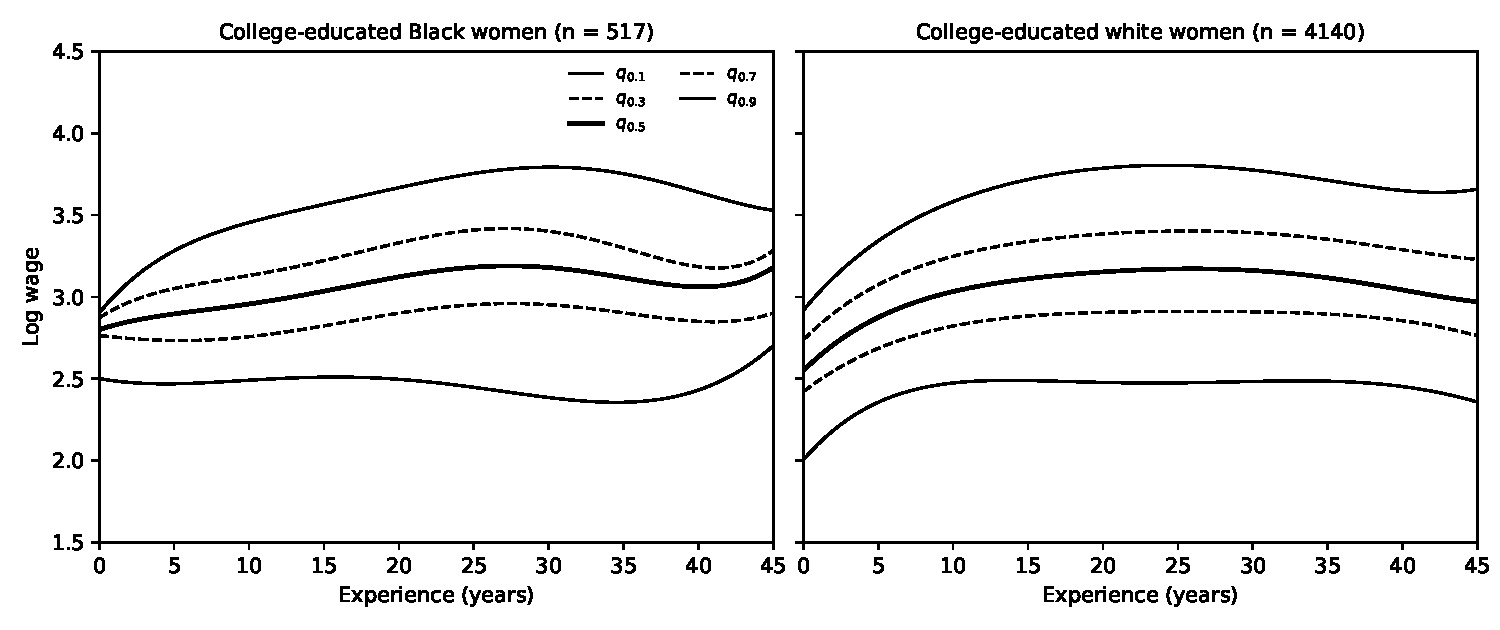
\includegraphics[width=\textwidth]{figures/ch24_16.pdf}
\end{center}
Fitted log wages:
\begin{center}
\small
\begin{tabular}{lcccccc|cccccc}
\toprule
 & \multicolumn{6}{c|}{Black women} & \multicolumn{6}{c}{white women}\\
experience & 0 & 5 & 10 & 20 & 30 & 40 & 0 & 5 & 10 & 20 & 30 & 40\\
\midrule
$q_{0.1}$ & 2.50 & 2.47 & 2.49 & 2.50 & 2.38 & 2.43 & 2.00 & 2.36 & 2.47 & 2.48 & 2.48 & 2.45\\
$q_{0.5}$ & 2.80 & 2.90 & 2.96 & 3.12 & 3.18 & 3.06 & 2.55 & 2.87 & 3.03 & 3.15 & 3.16 & 3.04\\
$q_{0.9}$ & 2.90 & 3.28 & 3.45 & 3.67 & 3.79 & 3.64 & 2.92 & 3.34 & 3.58 & 3.79 & 3.78 & 3.65\\
\bottomrule
\end{tabular}
\end{center}
\emph{Findings.}  For both groups the median profile rises by about 30--60 log points over the first 20--30 years and then
declines slightly.  The quantile functions fan out with experience, as in Figure 24.6: the 90--10 gap grows from
$0.4$ (Black) and $0.9$ (white) at entry to about $1.2$--$1.4$ log points after 20--30 years.  So wage heterogeneity increases more
than proportionately with experience.

\emph{Differences.}  At the top of the distribution the two profiles are very similar ($q_{0.9}\approx3.8$ at 30 years for both).  At
the bottom they differ.  The 10th percentile for Black women is essentially flat at about $2.5$ (no wage growth
with experience), whereas for white women it rises by almost 50 log points over the first ten years from a
lower starting value.  The higher entry values for Black women at low quantiles should be interpreted
cautiously: with only 517 observations the 5th-order polynomial is imprecise, especially at the
boundaries.  The flat bottom quantile nonetheless suggests that low-wage Black college-educated women
experience little wage progression, consistent with the book's observation that the lowest quantile
peaks early.
\end{ex}

%% ===========================================================================
%% Chapter 25. Binary Choice
%% ===========================================================================
\solchapter{25}{Binary Choice}

\begin{center}
\begin{minipage}{0.86\textwidth}
\small
Solutions to all 19 exercises of Chapter 25 of Bruce E.\ Hansen, \emph{Econometrics}
(Princeton University Press, 2022).  The empirical exercises use \texttt{cps09mar} (full-time workers, March 2009).
Probit models are estimated by maximum likelihood (Newton's method), with robust (sandwich)
standard errors.  Average partial effects (APE) are reported with delta-method standard errors; for dummy
regressors they are average discrete changes.
\end{minipage}
\end{center}

\bigskip
\hrule
\bigskip

Notation: $P[Y=1\given X]=G(X'\beta)$ with $G$ symmetric ($G(-u)=1-G(u)$), density $g=G'$, $Z=X$ if $Y=1$ and $Z=-X$ if $Y=0$,
$h(u)=\frac{d}{du}\log G(u)$ and $H(u)=-\frac{d^{2}}{du^{2}}\log G(u)$.

%%---------------------------------------------------------------------------
\begin{ex}{25.1}
Jacob's variable is $1-Y$, and $P[1-Y=1\given X]=1-\Phi(X'\beta)=\Phi(-X'\beta)$.  His log-likelihood at $b$ equals Emily's at $-b$, so his
MLE is exactly $-\wh\beta$: every coefficient, including the intercept, flips sign, and the standard errors are identical.
Marginal effects also flip sign.  (This uses the symmetry of the link, so it holds for logit too but not for
asymmetric links such as the complementary log-log.)
\end{ex}

%%---------------------------------------------------------------------------
\begin{ex}{25.2}
With $X^{*}=X/1000$ the index is $X\beta=X^{*}(1000\beta)$, so the likelihood is the same function after reparameterization.  By
invariance of the MLE, Julie's coefficient on that regressor is exactly $1000$ times Jackson's (standard error also
$\times1000$, $t$-ratio unchanged).  All other coefficients, fitted probabilities and marginal effects per dollar are
identical.
\end{ex}

%%---------------------------------------------------------------------------
\begin{ex}{25.3}
With $P(X)=P[Y=1\given X]$ and $e=Y-P(X)$: if $Y=1$ (probability $P(X)$) then $e=1-P(X)$; if $Y=0$ (probability $1-P(X)$) then $e=-P(X)$, which is
(25.1).  Then $\E[e\given X]=P(1-P)+(1-P)(-P)=0$ and
\[
  \var[e\given X]=\E[e^{2}\given X]=P(1-P)^{2}+(1-P)P^{2}=P(1-P)\bigl[(1-P)+P\bigr]=P(X)\bigl(1-P(X)\bigr),
\]
which is (25.2).
\end{ex}

%%---------------------------------------------------------------------------
\begin{ex}{25.4}
$\pi(Y\given X)=G(X'\beta)^{Y}\bigl(1-G(X'\beta)\bigr)^{1-Y}=G(X'\beta)^{Y}G(-X'\beta)^{1-Y}$ by symmetry.  If $Y=1$ this equals $G(X'\beta)=G(Z'\beta)$; if $Y=0$ it equals
$G(-X'\beta)=G(Z'\beta)$.
\end{ex}

%%---------------------------------------------------------------------------
\begin{ex}{25.5}
\textbf{(a)}  $\Lambda'(x)=e^{-x}/(1+e^{-x})^{2}=\Lambda(x)\cdot\dfrac{e^{-x}}{1+e^{-x}}=\Lambda(x)(1-\Lambda(x))$.
\textbf{(b)}  $\frac{d}{dx}\log\Lambda=\Lambda'/\Lambda=1-\Lambda$.
\textbf{(c)}  $-\frac{d}{dx}(1-\Lambda)=\Lambda'=\Lambda(1-\Lambda)$.
\textbf{(d)}  $0<\Lambda(1-\Lambda)\le\frac14$ since $p(1-p)\le\frac14$ on $[0,1]$; in particular $|H_{\rm logit}|\le1$.
\end{ex}

%%---------------------------------------------------------------------------
\begin{ex}{25.6}
\textbf{(a)}  $\frac{d}{dx}\log\Phi(x)=\phi(x)/\Phi(x)=\lambda(x)$.
\textbf{(b)}  Using $\phi'(x)=-x\phi(x)$,
\[
  -\frac{d}{dx}\lambda(x)=-\frac{\phi'(x)\Phi(x)-\phi(x)^{2}}{\Phi(x)^{2}}=\frac{x\phi(x)}{\Phi(x)}+\frac{\phi(x)^{2}}{\Phi(x)^{2}}=\lambda(x)\bigl(x+\lambda(x)\bigr).
\]
\end{ex}

%%---------------------------------------------------------------------------
\begin{ex}{25.7}
\textbf{(a)}  $\ell_n(\beta)=\sum_i\log G(Z_i'\beta)$, so by the chain rule $S_n(\beta)=\sum_iZ_ih(Z_i'\beta)$.  Differentiating again,
$\bs H_n(\beta)=-\sum_iZ_iZ_i'h'(Z_i'\beta)=\sum_iZ_iZ_i'H(Z_i'\beta)$, and $Z_iZ_i'=X_iX_i'$ because $Z_i=\pm X_i$.

\textbf{(b)}  For any $a\ne0$, $a'\bs H_n(\beta)a=\sum_i(a'X_i)^{2}H(Z_i'\beta)\ge0$, with equality only if $a'X_i=0$ for all $i$.  Given full rank $\sum X_iX_i'>0$
this is excluded, so $\bs H_n(\beta)>0$ for every $\beta$.

\textbf{(c)}  The Hessian of $\ell_n$ is $-\bs H_n(\beta)$, negative definite at every $\beta$, so $\ell_n$ is strictly concave on $\R^{k}$.  Any stationary point is
the unique global maximizer.  (A maximizer exists unless the data are perfectly separated.)
\end{ex}

%%---------------------------------------------------------------------------
\begin{ex}{25.8}
$0=\E[Zh(Z'\beta_0)]$.  Writing out the two cases, $Zh(Z'\beta)=X\bigl[Yg/G-(1-Y)g/(1-G)\bigr]$ with $g$ and $G$ evaluated at $X'\beta$.  This
simplifies to
\[
  \E\!\left[X\,\frac{g(X'\beta_0)}{G(X'\beta_0)\bigl(1-G(X'\beta_0)\bigr)}\bigl(Y-G(X'\beta_0)\bigr)\right]=0 ,
\]
a weighted orthogonality condition between the regressors and the ``residual'' $Y-G(X'\beta_0)$.
\end{ex}

%%---------------------------------------------------------------------------
\begin{ex}{25.9}
For the logit $g/(\Lambda(1-\Lambda))=1$, so $\displaystyle\sum_{i=1}^{n}X_i\bigl(Y_i-\Lambda(X_i'\wh\beta_{\rm logit})\bigr)=0$.  In particular, with an intercept, the average fitted
probability equals the sample frequency $\ol Y$.
\end{ex}

%%---------------------------------------------------------------------------
\begin{ex}{25.10}
$\displaystyle\sum_{i=1}^{n}X_i\frac{\phi(X_i'\wh\beta)}{\Phi(X_i'\wh\beta)\bigl(1-\Phi(X_i'\wh\beta)\bigr)}\bigl(Y_i-\Phi(X_i'\wh\beta)\bigr)=0$, or equivalently $\sum_iX_i\lambda(Z_i'\wh\beta)q_i=0$ with $q_i=2Y_i-1$.
\end{ex}

%%---------------------------------------------------------------------------
\begin{ex}{25.11}
By symmetry $h(-u)=g(u)/(1-G(u))$, so $h(Z'\beta)=Y\,g/G+(1-Y)\,g/(1-G)$ (all at $X'\beta$).  Squaring, the cross term vanishes because
$Y(1-Y)=0$:
\[
  h(Z'\beta)^{2}=\frac{g^{2}}{G^{2}}Y+\frac{g^{2}}{(1-G)^{2}}(1-Y)=\frac{g^{2}(Y-G)^{2}}{G^{2}(1-G)^{2}} .
\]
The last equality checks both cases: $Y=1$ gives $g^{2}(1-G)^{2}/(G^{2}(1-G)^{2})=g^{2}/G^{2}$ and $Y=0$ gives $g^{2}G^{2}/(G^{2}(1-G)^{2})=g^{2}/(1-G)^{2}$.  For the logit
$g=\Lambda(1-\Lambda)$, so the ratio $g^{2}/(G^{2}(1-G)^{2})$ is one and $h(Z'\beta)^{2}=(Y-\Lambda(X'\beta))^{2}$.
\end{ex}

%%---------------------------------------------------------------------------
\begin{ex}{25.12}
By (25.1), $Y=\Phi(X'\beta)+e$ with $\E[e\given X]=0$ is a nonlinear regression, so
\[
  \wh\beta_{\rm nlls}=\argmin_\beta\sum_{i=1}^{n}\bigl(Y_i-\Phi(X_i'\beta)\bigr)^{2},\qquad \text{first-order condition }\ \sum_iX_i\phi(X_i'\wh\beta)\bigl(Y_i-\Phi(X_i'\wh\beta)\bigr)=0 .
\]
It is consistent under correct specification.  Because $\var[e\given X]=\Phi(1-\Phi)$ is heteroskedastic, standard errors must use the
robust formula (23.6) with $\wh m_{\theta i}=X_i\phi(X_i'\wh\beta)$.  NLLS is less efficient than the MLE.  Weighted NLLS with weights
$1/\{\wt\Phi_i(1-\wt\Phi_i)\}$ from a first-step estimate has the MLE's first-order condition (Exercise 25.10), and iterating it
reproduces the MLE (iteratively reweighted least squares).
\end{ex}

%%---------------------------------------------------------------------------
\begin{ex}{25.13}
\textbf{(a)}  With $e_1=\rho e_2+\varepsilon$ and $e_2=Y_2-X'\gamma_1-Z'\gamma_2$, substitute into the structural equation:
$Y_1^{*}=X'\beta_1+Y_2\beta_2+\rho(Y_2-X'\gamma_1-Z'\gamma_2)+\varepsilon=\mu(\theta)+\varepsilon$.

\textbf{(b)}  Conditional on $(X,Z)$, $(e_1,e_2)$ is bivariate normal and $\varepsilon=e_1-\rho e_2$ with $\rho=\sigma_{12}/\sigma_2^{2}$ has $\cov(\varepsilon,e_2)=\sigma_{12}-\rho\sigma_2^{2}=0$.
Jointly normal and uncorrelated implies independent.  As $Y_2=X'\gamma_1+Z'\gamma_2+e_2$ is a function of $(X,Z,e_2)$, $\varepsilon$ is also
independent of $Y_2$ given $(X,Z)$.

\textbf{(c)}  Conditional on $(Y_2,X,Z)$, $\mu(\theta)$ is fixed and $\varepsilon\sim N(0,\sigma_\varepsilon^{2})$ with $\sigma_\varepsilon^{2}=\var(e_1)-\rho^{2}\sigma_2^{2}=1-\sigma_{12}^{2}/\sigma_2^{2}$ (by (b)).  Hence $Y_1^{*}\given(Y_2,X,Z)\sim N(\mu(\theta),\sigma_\varepsilon^{2})$
and $P[Y_1=1\given Y_2,X,Z]=\Phi(\mu(\theta)/\sigma_\varepsilon)$, which gives the likelihood in the text.
\end{ex}

%%---------------------------------------------------------------------------
\begin{ex}{25.14}
(For a binary choice model the observation rule should read $Y=\indic\{Y^{*}>0\}$.  As printed, $Y=Y^{*}\indic\{Y^{*}>0\}$ is a Tobit model,
in which $m$ and $\sigma^{2}$ are both identified.)

\textbf{(a)}  $P(x)=P[m(x)+e>0\given X=x]=\Phi\bigl(m(x)/\sigma(x)\bigr)$.

\textbf{(b)}  No.  Only the ratio $r(x)=m(x)/\sigma(x)=\Phi^{-1}(P(x))$ is identified: $(cm,c\sigma)$ for any function $c(x)>0$ gives the same response
probability.

\textbf{(c)}  Normalize $\sigma(x)\equiv1$.  Then $m(x)=\Phi^{-1}(P(x))$ is identified (equivalently, identify the ratio $m/\sigma$).

\textbf{(d)}  Not nonparametrically.  Any heteroskedastic model is observationally equivalent to a homoskedastic
one with $m^{*}=m/\sigma$, so ``allowing for heteroskedasticity'' adds nothing unless $m$ is restricted.  In a parametric
model, e.g.\ $m(x)=x'\beta$ with $\sigma(x)=\exp(z'\gamma)$, heteroskedasticity is identified only through the functional-form
restrictions, and it is better viewed as a more flexible model for the response probability.
\end{ex}

%%---------------------------------------------------------------------------
\begin{ex}{25.15}
$n=29{,}140$.  Only $2.25\%$ of men in this extract report union membership, far below the published 2009 U.S. rate of
about 12\%.  The \emph{union} indicator evidently captures only part of membership in these data, so it is best to
focus on relative magnitudes.
\begin{center}
\begin{tabular}{lcccc}
\toprule
 & coefficient & s.e. & APE (pp) & s.e.\\
\midrule
intercept & $-1.954$ & $(0.100)$ & & \\
age & $0.0079$ & $(0.0014)$ & $0.04$ & $(0.01)$\\
education & $-0.0255$ & $(0.0057)$ & $-0.14$ & $(0.03)$\\
Black & $-0.054$ & $(0.060)$ & $-0.27$ & $(0.29)$\\
Hispanic & $-0.298$ & $(0.059)$ & $-1.28$ & $(0.20)$\\
\bottomrule
\end{tabular}
\end{center}
Membership increases with age (seniority, and declining unionization of younger cohorts) and decreases with
education: unionized jobs are concentrated in blue-collar occupations.  Hispanic men are about $1.3$ percentage
points less likely to be members, over half the base rate, even controlling for education and age.  There is no
significant difference for Black men.
\end{ex}

%%---------------------------------------------------------------------------
\begin{ex}{25.16}
$n=21{,}602$, membership rate $2.0\%$.
\begin{center}
\begin{tabular}{lcccc}
\toprule
 & coefficient & s.e. & APE (pp) & s.e.\\
\midrule
intercept & $-3.095$ & $(0.141)$ & & \\
age & $0.0101$ & $(0.0017)$ & $0.05$ & $(0.01)$\\
education & $0.0435$ & $(0.0080)$ & $0.21$ & $(0.04)$\\
Black & $-0.047$ & $(0.062)$ & $-0.22$ & $(0.28)$\\
Hispanic & $-0.148$ & $(0.070)$ & $-0.63$ & $(0.27)$\\
\bottomrule
\end{tabular}
\end{center}
The age effect is similar to men's, but the education effect has the \emph{opposite} sign: more educated women are
more likely to be union members.  This reflects the composition of female union membership, concentrated in the
public sector and in professions such as teaching and nursing, whereas male membership is concentrated in
manual occupations.  The Hispanic gap is smaller than for men but still significant ($-0.6$ pp); Black women do not
differ significantly.
\end{ex}

%%---------------------------------------------------------------------------
\begin{ex}{25.17}
$n=5199$, $63\%$ married.  Following Figure 25.1 we use a probit in a quadratic spline of $\text{age}/100$ with knots at 40 and 60.  This
gives a smooth, flexible age profile that can rise, plateau and fall, while the probit link keeps probabilities
in $[0,1]$.  The spline improves substantially on a quadratic probit (AIC $6525$ versus $6560$).
\begin{center}
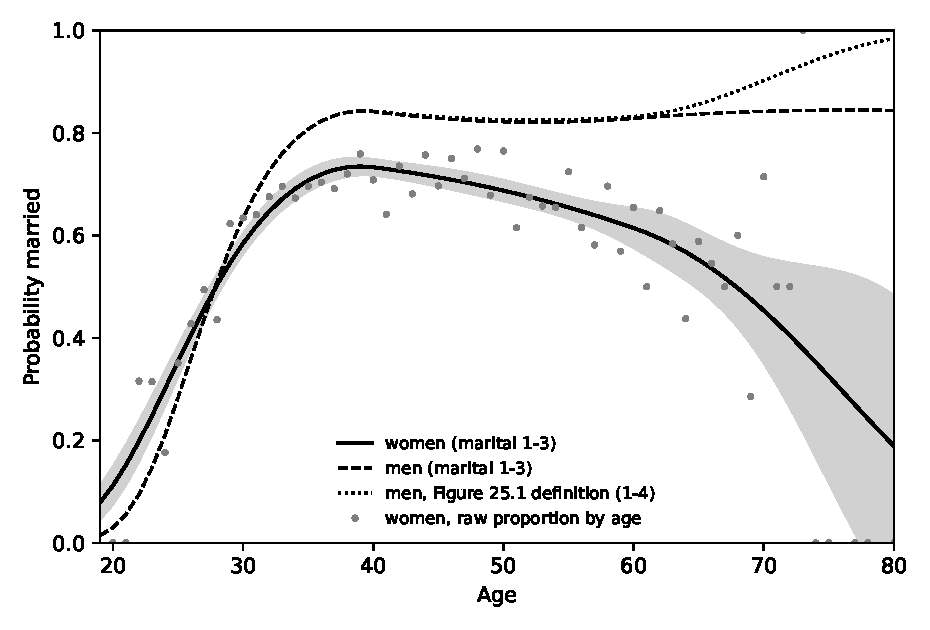
\includegraphics[width=0.75\textwidth]{figures/ch25_17.pdf}
\end{center}
Estimated probabilities: $0.20$ at age 22, $0.35$ at 25, $0.58$ at 30, $0.71$ at 35, $0.73$ at 40, $0.69$ at 50, $0.61$ at 60, $0.45$ at 70.

\emph{Comparison with men.}  College-educated men (same definition, $n=6441$): $0.09$ at 22, $0.28$ at 25, $0.64$ at 30, $0.84$ at 40, and about $0.83$
thereafter.  Women marry earlier (higher probabilities before about 27), but their probability plateaus lower
($0.73$ versus $0.84$) and declines steadily after 40, whereas men's stays flat.  The decline for women reflects
divorce and widowhood (widows are not counted as married here) with less remarriage, and women's
longer life expectancy.

\rmk{Coding note.  Figure 25.1's code defines ``married'' as marital $\le4$, which includes widowed (code 4).  With that
definition the men's curve rises toward one at old ages (dotted line, $0.98$ at 80), an artefact of counting widowers as
married.  With the exercise's definition (codes 1--3) it is flat after 40.}
\end{ex}

%%---------------------------------------------------------------------------
\begin{ex}{25.18}
Probit with the age spline of Exercise 25.17 (not reported; coefficients on $a=\text{age}/100$: $44.9$, $-57.0$, $60.5$, $-4.7$), $n=29{,}140$, $72\%$ married:
\begin{center}
\begin{tabular}{lcccc}
\toprule
 & coefficient & s.e. & APE (pp) & s.e.\\
\midrule
education & $0.0263$ & $(0.0031)$ & $0.78$ & $(0.09)$\\
Black & $-0.498$ & $(0.029)$ & $-16.4$ & $(1.0)$\\
Hispanic & $0.005$ & $(0.025)$ & $0.1$ & $(0.7)$\\
\bottomrule
\end{tabular}
\end{center}
For a white non-Hispanic man with mean education the probability of being married is $0.39$ at 25, $0.65$ at 30, $0.82$ at 40,
and stays around $0.81$--$0.84$ through 70.  Each additional year of education raises it by about $0.8$ points.  Black
men are 16 points less likely to be married, a very large gap given the controls.  Hispanic men do not differ from white men.
\end{ex}

%%---------------------------------------------------------------------------
\begin{ex}{25.19}
$n=21{,}602$, $59\%$ married.
\begin{center}
\begin{tabular}{lcccc}
\toprule
 & coefficient & s.e. & APE (pp) & s.e.\\
\midrule
education & $0.0256$ & $(0.0035)$ & $0.92$ & $(0.13)$\\
Black & $-0.645$ & $(0.027)$ & $-24.1$ & $(1.0)$\\
Hispanic & $-0.132$ & $(0.027)$ & $-4.8$ & $(1.0)$\\
\bottomrule
\end{tabular}
\end{center}
Profile for white non-Hispanic women with mean education: $0.39$ at 25, $0.58$ at 30, $0.72$ at 40, $0.69$ at 50, $0.62$ at 60 and $0.44$ at 70.  It peaks
around 40 and then declines, unlike men's.  The education effect is similar to men's (about $0.9$ points per
year).  The Black gap is even larger for women ($-24$ points), and Hispanic women are about 5 points less likely to be
married, whereas Hispanic men are not.  All results describe full-time workers, the population of the \texttt{cps09mar}
extract, so they combine marriage patterns with selection into full-time work, which differs by sex
and marital status.
\end{ex}

%% ===========================================================================
%% Chapter 26. Multiple Choice
%% ===========================================================================
\solchapter{26}{Multiple Choice}

\begin{center}
\begin{minipage}{0.86\textwidth}
\small
Solutions to all 18 exercises of Chapter 26 of Bruce E.\ Hansen, \emph{Econometrics}
(Princeton University Press, 2022).  The empirical exercises use \texttt{cps09mar} and \texttt{Koppelman} (2779 business travellers
choosing among train, air, bus and car).  All models were programmed directly and estimated by (simulated)
maximum likelihood, with standard errors from the inverse numerical Hessian.
\begin{itemize}[leftmargin=*]
\item Simple multinomial probit (iid normal errors): exact one-dimensional Gauss--Hermite quadrature.
\item Mixed logit: 400 (or 200) Halton draws per traveller.
\item General multinomial probit: the GHK simulator with 300 Halton draws.
\end{itemize}
The conditional logit and simple probit columns of Table 26.1 are reproduced exactly.  The nested and mixed
logit columns are reproduced up to three apparent typos, discussed in Exercises 26.16 and 26.17, and the
general probit column up to simulation error (Exercise 26.18).
\end{minipage}
\end{center}

\bigskip
\hrule
\bigskip

Notation: $P_j$ denotes response probabilities, $\mu_j=w'\beta_j+x_j'\gamma$ the systematic utility of alternative $j$, and $J$ the base alternative.

%%---------------------------------------------------------------------------
\begin{ex}{26.1}
Each term $\exp(x'\beta_j)$ is strictly positive, so $P_j(x)>0$.  The numerator is one of the positive terms of the denominator,
so $P_j(x)\le1$ (strictly less if $J\ge2$).  Summing over $j$, the numerators add up to the common denominator, so $\sum_jP_j(x)=1$.
\end{ex}

%%---------------------------------------------------------------------------
\begin{ex}{26.2}
Divide numerator and denominator by $\exp(x'\beta_J)$:
\[
  P_j(x)=\frac{\exp\bigl(x'(\beta_j-\beta_J)\bigr)}{\sum_{\ell=1}^{J}\exp\bigl(x'(\beta_\ell-\beta_J)\bigr)} .
\]
Adding a common vector to every $\beta_j$ leaves all probabilities unchanged, which is why one alternative must be normalized, e.g.\ $\beta_J=0$.
\end{ex}

%%---------------------------------------------------------------------------
\begin{ex}{26.3}
Write $D(x)=\sum_\ell\exp(x'\beta_\ell)$, so that $\partial D/\partial x=\sum_\ell\beta_\ell\exp(x'\beta_\ell)$.  By the quotient rule,
\[
  \frac{\partial P_j}{\partial x}=\frac{\beta_j\exp(x'\beta_j)}{D}-\frac{\exp(x'\beta_j)}{D}\cdot\frac{\sum_\ell\beta_\ell\exp(x'\beta_\ell)}{D}=P_j(x)\Bigl(\beta_j-\sum_{\ell=1}^{J}\beta_\ell P_\ell(x)\Bigr).
\]
\end{ex}

%%---------------------------------------------------------------------------
\begin{ex}{26.4}
Let $U_j=\mu_j+\varepsilon_j$ with $\varepsilon_j$ i.i.d.\ Type I extreme value, $F(\varepsilon)=\exp(-e^{-\varepsilon})$, $f(\varepsilon)=e^{-\varepsilon}\exp(-e^{-\varepsilon})$.  Conditioning on $\varepsilon_j$,
\[
  P_j=\int f(\varepsilon)\prod_{\ell\ne j}F(\varepsilon+\mu_j-\mu_\ell)\,d\varepsilon=\int e^{-\varepsilon}\exp\Bigl(-e^{-\varepsilon}\sum_{\ell=1}^{J}e^{\mu_\ell-\mu_j}\Bigr)d\varepsilon .
\]
With $t=e^{-\varepsilon}$ this is $\int_0^\infty\exp(-tS)\,dt=1/S$, where $S=\sum_\ell e^{\mu_\ell-\mu_j}$.  Hence $P_j=\exp(\mu_j)/\sum_\ell\exp(\mu_\ell)$, which is (26.8) with $\mu_j=w'\beta_j+x_j'\gamma$.  (This is
Theorem 26.1 with $\tau=1$ applied to general indices $\mu_j$.)
\end{ex}

%%---------------------------------------------------------------------------
\begin{ex}{26.5}
$x_j$ enters only $\mu_j$, with $\partial\mu_j/\partial x_j=\gamma$.  Hence
\[
  \frac{\partial P_j}{\partial x_j}=\gamma\frac{e^{\mu_j}}{D}-\frac{e^{\mu_j}}{D}\cdot\frac{\gamma e^{\mu_j}}{D}=\gamma P_j(1-P_j),\qquad
  \frac{\partial P_j}{\partial x_\ell}=-\frac{e^{\mu_j}}{D}\cdot\frac{\gamma e^{\mu_\ell}}{D}=-\gamma P_jP_\ell\quad(\ell\ne j).
\]
\end{ex}

%%---------------------------------------------------------------------------
\begin{ex}{26.6}
Divide numerator and denominator by $\exp(w'\beta_J+x_J'\gamma)$:
\[
  P_j(w,x)=\frac{\exp\bigl(w'(\beta_j-\beta_J)+(x_j-x_J)'\gamma\bigr)}{\sum_\ell\exp\bigl(w'(\beta_\ell-\beta_J)+(x_\ell-x_J)'\gamma\bigr)} .
\]
Only utility differences matter.  Adding a constant to all $x_j$ (e.g.\ a common price change) has no effect, and the $\beta_j$ are
identified only relative to the base.
\end{ex}

%%---------------------------------------------------------------------------
\begin{ex}{26.7}
By (26.9), $\text{AME}_{jj}=\E\bigl[\gamma P_j(W,X)(1-P_j(W,X))\bigr]$.  The plug-in estimator is
\[
  \wh{\text{AME}}_{jj}=\wh\gamma\,\frac1n\sum_{i=1}^{n}\wh P_j(W_i,X_i)\bigl(1-\wh P_j(W_i,X_i)\bigr),\qquad \wh P_j(W_i,X_i)=P_j(W_i,X_i\given\wh\theta),
\]
with standard errors from the delta method, i.e.\ the gradient of this smooth function of $\wh\theta$ times the estimated covariance of $\wh\theta$.
\end{ex}

%%---------------------------------------------------------------------------
\begin{ex}{26.8}
The two probabilities in (26.8) share the denominator $\sum_\ell\exp(w'\beta_\ell+x_\ell'\gamma)$, which cancels:
$P_j/P_\ell=\exp(w'\beta_j+x_j'\gamma)/\exp(w'\beta_\ell+x_\ell'\gamma)$.
\end{ex}

%%---------------------------------------------------------------------------
\begin{ex}{26.9}
Set $w'\beta_j=w'\beta_\ell=0$ in (26.11): $P_j/P_\ell=\exp(x_j'\gamma)/\exp(x_\ell'\gamma)=\exp\bigl((x_j-x_\ell)'\gamma\bigr)$.  The odds between two alternatives depend only on
the difference in their attributes, not on any other alternative: independence of irrelevant alternatives.
\end{ex}

%%---------------------------------------------------------------------------
\begin{ex}{26.10}
By Theorem 26.2, $P_{jk}=P_{k\given j}P_j$, and the group probability cancels:
\[
  \frac{P_{jk}}{P_{j\ell}}=\frac{P_{k\given j}}{P_{\ell\given j}}=\exp\Bigl(\frac{\mu_{jk}-\mu_{j\ell}}{\tau_j}\Bigr).
\]
This depends only on the utilities of $k$ and $\ell$.  IIA therefore holds within a nest: a change in an alternative in another nest
(e.g.\ a cheaper air fare) changes the probabilities of train and bus in the same proportion, so their relative odds are
unchanged.  The nested logit relaxes IIA only across nests.
\end{ex}

%%---------------------------------------------------------------------------
\begin{ex}{26.11}
The group probabilities share a denominator, so
\[
  \frac{P_j}{P_\ell}=\frac{\bigl(\sum_{m}\exp(\mu_{jm}/\tau_j)\bigr)^{\tau_j}}{\bigl(\sum_{m}\exp(\mu_{\ell m}/\tau_\ell)\bigr)^{\tau_\ell}}=\frac{\exp(\tau_jI_j)}{\exp(\tau_\ell I_\ell)},\qquad I_j=\log\sum_m\exp(\mu_{jm}/\tau_j),
\]
which involves only the alternatives in groups $j$ and $\ell$ (through their inclusive values $I_j$, $I_\ell$).  IIA holds at the group level:
the relative odds of two nests are unaffected by changes in a third nest.  Within the model, substitution
patterns are flexible only in the sense that alternatives in the same nest are closer substitutes.
\end{ex}

%%---------------------------------------------------------------------------
\begin{ex}{26.12}
Following Figure 26.1 we use college graduates, four categories (married, which includes widowed as in the book's
coding; separated; divorced; never married), and a quadratic spline in $\text{age}/100$ with a knot at 40.  Samples: men $n=6441$,
women $n=5199$.
\begin{center}
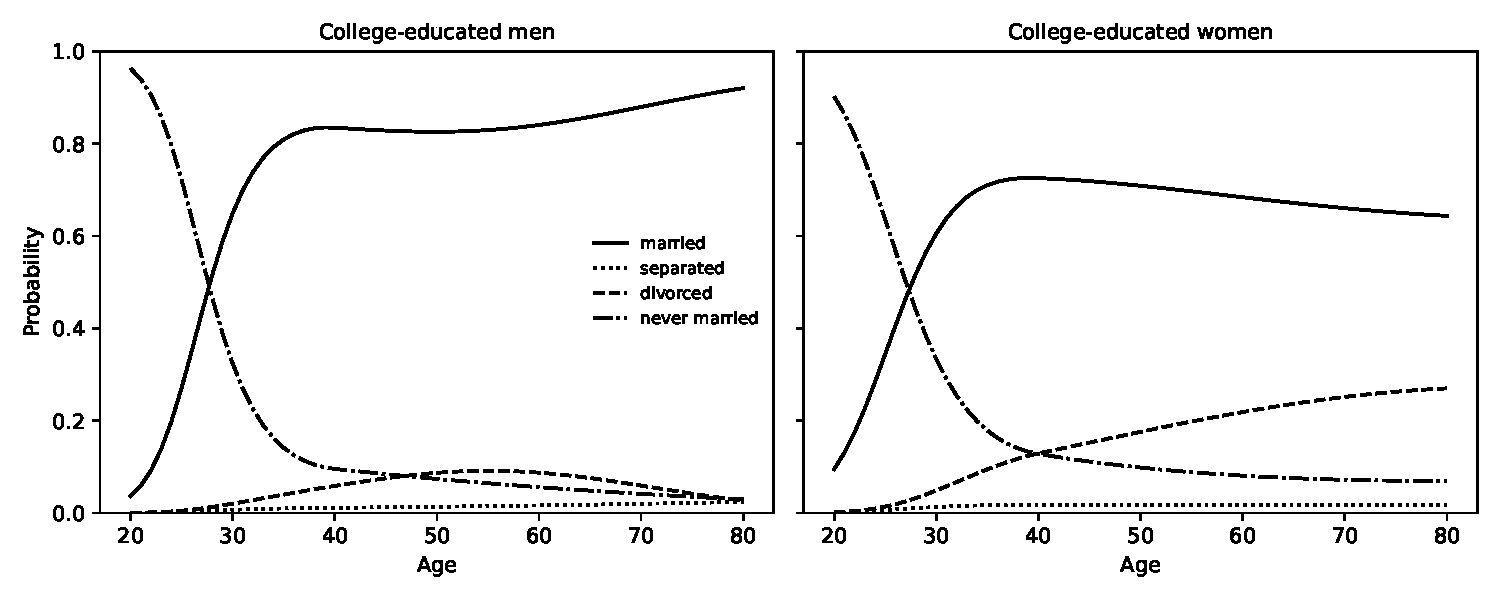
\includegraphics[width=\textwidth]{figures/ch26_12.pdf}
\end{center}
\begin{center}
\small
\begin{tabular}{lcccc|cccc}
\toprule
 & \multicolumn{4}{c|}{men} & \multicolumn{4}{c}{women}\\
age & married & separated & divorced & never & married & separated & divorced & never\\
\midrule
25 & 0.27 & 0.00 & 0.01 & 0.72 & 0.35 & 0.01 & 0.01 & 0.64\\
30 & 0.65 & 0.01 & 0.02 & 0.32 & 0.61 & 0.01 & 0.05 & 0.33\\
40 & 0.84 & 0.01 & 0.06 & 0.10 & 0.73 & 0.02 & 0.13 & 0.13\\
50 & 0.83 & 0.01 & 0.09 & 0.07 & 0.71 & 0.02 & 0.18 & 0.10\\
60 & 0.84 & 0.02 & 0.09 & 0.06 & 0.68 & 0.02 & 0.22 & 0.08\\
70 & 0.88 & 0.02 & 0.06 & 0.04 & 0.66 & 0.02 & 0.25 & 0.07\\
\bottomrule
\end{tabular}
\end{center}
For both sexes the probability of never having married falls steeply between 25 and 40.  Men marry somewhat later
(72\% never married at 25 versus 64\% for women) but then reach a much higher married share ($0.84$ versus $0.73$ at 40).
After 40 the profiles diverge.  For men the married probability stays around $0.83$--$0.88$ and the divorced share peaks
below 10\% and then falls (remarriage).  For women the married probability declines slowly and the divorced share
keeps rising, to 25\% at 70.  Divorced women are much less likely than men to remarry.  Separation is rare for both.
\end{ex}

%%---------------------------------------------------------------------------
\begin{ex}{26.13}
$n=6645$ (married $48.8\%$, separated $2.7\%$, divorced $6.5\%$, never married $42.0\%$); base category: married.
\begin{center}
\begin{tabular}{lccc}
\toprule
 & separated & divorced & never married\\
\midrule
age & $-0.041$ $(0.019)$ & $0.054$ $(0.014)$ & $-0.195$ $(0.007)$\\
education & $-0.247$ $(0.028)$ & $-0.123$ $(0.020)$ & $-0.023$ $(0.012)$\\
constant & $1.68$ $(0.66)$ & $-1.91$ $(0.51)$ & $5.74$ $(0.24)$\\
\bottomrule
\end{tabular}
\end{center}
Average marginal effects (probability points per year): age $+3.3$ (married), $+0.1$ (separated), $+0.8$ (divorced), $-4.1$
(never married); education $+1.2$ (married), $-0.6$ (separated), $-0.6$ (divorced), $+0.05$ (never married).

\emph{Interpretation.}  Among young women, each year of age moves about four points of probability from never married to
married (and a little to divorced), the transition into marriage in the late twenties and early thirties.
Education barely changes the probability of never having married, but among those who have married it strongly
reduces separation and divorce.  At age 35, for example, $14.4\%$ of women with 12 years of schooling are divorced and $4.3\%$
separated, versus $9.7\%$ and $1.8\%$ with 16 years, so college-educated women are more often currently married ($0.72$ versus $0.65$).
\end{ex}

%%---------------------------------------------------------------------------
\begin{ex}{26.14}
All women ($n=21{,}602$), the same four categories and age spline, with alternative-specific coefficients and married as the
base.  The multinomial logit has log-likelihood $-19823.24$.

\emph{Choosing the nests.}  Alternatives that are close substitutes, i.e.\ share unobserved determinants, should be
grouped together.  Separated and divorced are both ``formerly married'' states (separation is often a step
towards divorce), so the natural structure is $\{\text{married}\}$, $\{\text{never married}\}$, $\{\text{separated},\text{divorced}\}$, with one dissimilarity
parameter.  We also tried $\{\text{married},\text{separated}\}$ versus $\{\text{divorced},\text{never married}\}$ (legally married or not) and $\{\text{ever married}\}$ versus
$\{\text{never married}\}$.  Results:
\begin{center}
\small
\begin{tabular}{lccc}
\toprule
nests & $\wh\tau$ (s.e.) & log-likelihood & LR vs.\ MNL\\
\midrule
$\{M\}$, $\{N\}$, $\{S,D\}$ & $180$ $(109)$ & $-19814.35$ & $17.8$\\
$\{M,S\}$, $\{D,N\}$ & $38.8$ $(34.0)$, $2.09$ $(0.72)$ & $-19820.66$ & $5.2$\\
$\{M,S,D\}$, $\{N\}$ & $1.06$ $(7.8)$ & $-19823.24$ & $0.0$\\
\bottomrule
\end{tabular}
\end{center}
None of the groupings supports a nested structure.  Consistency with random utility maximization requires $0<\tau\le1$, and
every unrestricted estimate exceeds one.  Restricting $\tau\le1$, the profile likelihood for the preferred nesting increases
monotonically in $\tau$ ($-19823.86$ at $\tau=0.3$, $-19823.59$ at $0.6$, $-19823.33$ at $0.9$, $-19823.24$ at $1$).  So the constrained MLE is $\tau=1$, i.e.\ the
multinomial logit.  With only individual-specific regressors (age) the dissimilarity parameter is also very weakly
identified, as the huge standard errors show.  The data give no reason to depart from IIA here.  A nested model
could still be motivated a priori, but it cannot be supported empirically with these regressors.
\end{ex}

%%---------------------------------------------------------------------------
\bigskip
\noindent\textbf{The transportation application (Exercises 26.15--26.18).}  The \texttt{Koppelman} data contain $n=2779$
business travellers, each choosing among train, air, bus and car.  Alternative-varying regressors are cost (dollars), in-vehicle
time \texttt{intime} and out-of-vehicle time \texttt{outtime} (minutes).  Individual-specific regressors are income and a dummy
for urban origin/destination, which enter with alternative-specific coefficients (train is the base).  All specifications below include
the nine alternative-specific coefficients (income, urban and a constant for air, bus and car).  The tables report only the cost and
time coefficients, as the exercises request.  LR denotes a likelihood ratio statistic.

%%---------------------------------------------------------------------------
\begin{ex}{26.15}
\begin{center}
\small
\begin{tabular}{lcccc}
\toprule
 & (a) Table 26.1 & (b) $+$outtime & (c) time $=$ in$+$out & (d) logs\\
\midrule
cost & $-0.0218$ $(0.0035)$ & $-0.0150$ $(0.0037)$ & $-0.0153$ $(0.0037)$ & $-4.67$ $(0.26)$\\
intime & $-0.0149$ $(0.0007)$ & $-0.0178$ $(0.0008)$ & & $-0.44$ $(0.25)$\\
outtime & & $-0.0309$ $(0.0027)$ & & \\
time & & & $-0.0176$ $(0.0008)$ & \\
car constant & $1.86$ $(0.19)$ & $-0.96$ $(0.30)$ & $0.25$ $(0.19)$ & $1.62$ $(0.20)$\\
log-likelihood & $-2100.6$ & $-2026.8$ & $-2040.8$ & $-2082.3$\\
\bottomrule
\end{tabular}
\end{center}
In (d) the coefficients are on $\log(\text{cost})$ and $\log(\text{intime})$.

\begin{enumerate}[label=(\alph*)]
\item Column (a) reproduces the conditional logit column of Table 26.1 exactly: cost $-0.022$, intime $-0.015$, and all
nine alternative-specific coefficients agree to the printed digits.  The implied value of in-vehicle time is $0.0149/0.0218=\$0.68$ per
minute, about $\$41$ per hour.
\item Out-of-vehicle time is highly significant ($t=-11.4$; LR $=147.6$ against (a)).  Its coefficient is $1.7$ times the in-vehicle
coefficient, the classic transportation finding that waiting and access time is valued well above riding time.  Controlling
for it, the cost coefficient falls by a third and the in-vehicle time coefficient rises slightly.  The implied values of time
are $\$1.19$/min ($\$71$/h) in-vehicle and $\$2.06$/min ($\$124$/h) out-of-vehicle.  The car constant swings from $+1.86$ to $-0.96$.  Car has no
out-of-vehicle time, so in (a) its constant was absorbing car's access-time advantage.
\item Model (c) is model (b) with the restriction $\gamma_{\rm in}=\gamma_{\rm out}$.  It fits much better than (a) but is rejected against (b):
LR $=2(2040.8-2026.8)=28.0$, against $\chi^2_1$ critical value $3.84$.  Adding the two times together is too restrictive, since travellers
dislike out-of-vehicle minutes more.
\item The log specification makes utility depend on proportional changes.  The cost coefficient $-4.67$ is now on
the elasticity scale: the own-cost elasticity of $P_j$ is $-4.67(1-P_j)$, e.g.\ about $-3.3$ for a mode with a $30\%$ share.  The log-time
coefficient becomes small and only marginally significant ($t=-1.7$).  Once cost enters in logs, relative cost differences
absorb most of what time was explaining.  The fit improves on (a) by 18.3 log-likelihood points with the same number
of parameters.  So among the two-regressor specifications the data prefer logs, but both are dominated by
specifications that include out-of-vehicle time.
\end{enumerate}
\end{ex}

%%---------------------------------------------------------------------------
\begin{ex}{26.16}
The model is the nested logit of Theorem 26.2.  Within group $g$ utilities are scaled by $1/\tau_g$, and the inclusive value is
$I_g=\log\sum_{k\in g}e^{\mu_k/\tau_g}$.  A singleton nest has no free $\tau$.  Consistency with random utility maximization requires
$0<\tau_g\le1$.
\begin{center}
\small
\begin{tabular}{lcccc}
\toprule
 & (a) Table 26.1 & (b) logs & (c) $\{C\},\{T,B,A\}$ & (d) $\{A\},\{T,B,C\}$\\
\midrule
cost & $-0.0014$ $(0.0016)$ & $-0.051$ $(0.009)$ & $-0.0265$ $(0.0028)$ & $-0.0333$ $(0.0055)$\\
intime & $-0.0054$ $(0.0010)$ & $0.018$ $(0.005)$ & $-0.0122$ $(0.0008)$ & $-0.0190$ $(0.0009)$\\
$\wh\tau$ & $0.236$ $(0.046)$ & $0.0057$ $(0.0010)$ & $0.664$ $(0.061)$ & $3.81$ $(0.62)$\\
log-likelihood & $-2044.4$ & $-2011.1$ & $-2091.5$ & $-2023.8$\\
\bottomrule
\end{tabular}
\end{center}
In (a) and (b) the groupings are $\{\text{car},\text{air}\}$ and $\{\text{train},\text{bus}\}$ with $\tau_{\rm train,bus}=1$, and $\wh\tau$ is $\tau_{\rm car,air}$.  In (c) and (d), $\wh\tau$ is the
parameter of the three-alternative nest.  In (b) the coefficients are on $\log(\text{cost})$ and $\log(\text{intime})$.  The conditional logit
log-likelihood is $-2100.6$.

\begin{enumerate}[label=(\alph*)]
\item With $\tau_{\rm train,bus}=1$ we reproduce the nested logit column of Table 26.1: intime $-0.005$, $\wh\tau_{\rm car,air}=0.24$ $(0.05)$, air income
$0.024$, bus coefficients $-0.049$, $-0.21$, $-1.55$, and car coefficients $0.017$, $-0.58$, $1.19$.  Two entries do not match:
\begin{itemize}[leftmargin=*]
\item The cost coefficient is $-0.0014$ $(0.0016)$, not $-0.011$ $(0.002)$.
\item The air--urban coefficient is $-0.28$ $(0.08)$, not $+0.28$ $(0.09)$.
\end{itemize}
Since every other coefficient agrees to the printed digits (which would be impossible if the cost coefficient really
differed by a factor of eight), these are almost certainly typos in the table ($-0.001$ misprinted as $-0.011$, and a dropped
minus sign).

\emph{Why the constraint is needed.}  Leaving $\tau_{\rm train,bus}$ free, the profile log-likelihood is bimodal:
\begin{center}
\small\setlength{\tabcolsep}{3.5pt}
\begin{tabular}{lccccccccc}
\toprule
$\tau_{\rm train,bus}$ & $0.1$ & $0.26$ & $0.5$ & $1$ & $1.5$ & $3$ & $10$ & $30$ & $100$\\
log-lik. & $-2045.8$ & $-2043.5$ & $-2043.9$ & $-2044.4$ & $-2044.5$ & $-2043.3$ & $-2038.5$ & $-2037.0$ & $-2037.9$\\
\bottomrule
\end{tabular}
\end{center}
There is a local maximum inside the admissible range, at $\tau_{\rm train,bus}=0.26$ $(0.14)$, but it is only $1.0$ log-likelihood points better than $\tau=1$.  The global
maximum is near $\tau\approx30$, far outside $(0,1]$, where the model is not a random utility model.  An unconstrained
optimizer therefore drifts to meaningless values.  The book imposes $\tau_{\rm train,bus}=1$, which the data do not reject
(LR $=1.9$ against the interior local maximum).

\emph{Interpretation.}  The car/air dissimilarity $0.24$ implies a correlation of about $1-0.24^2=0.94$ between the car and air shocks.  The
likelihood gain over conditional logit is large: LR $=112$.  With nesting, the cost coefficient becomes small and
insignificant, and the time coefficient falls by two-thirds.  Much of the apparent price and time sensitivity in conditional logit reflects IIA-forced
substitution patterns.  Within the nest, utilities are scaled by $1/\wh\tau\approx4.2$, so the within-nest cost and time sensitivities are
$-0.006$ and $-0.023$.
\item With logs, $\wh\tau_{\rm car,air}$ collapses to $0.006$.  The within-nest choice between car and air becomes almost deterministic
given the utilities.  The log-likelihood rises to $-2011.1$, but the log-intime coefficient is \emph{positive} and significant
($0.018$, or $0.018/0.0057=3.1$ within the nest).  A dissimilarity parameter at the edge of the parameter space together with a
wrong-signed time effect indicates a model that fits by near-perfect prediction within the $\{\text{car},\text{air}\}$
nest, not an economically meaningful specification.
\item \emph{Rationale:} car is private transport, while train, bus and air are common carriers with schedules, terminals and access
and egress time.  Their unobserved attributes (reliability, comfort, the inconvenience of fixed departure times) plausibly
move together.  The estimate $\wh\tau=0.66$ lies in $(0,1)$, so the model is RUM-consistent, and conditional logit is rejected (LR $=18.2$).
But the fit is much worse than the $\{\text{car},\text{air}\}$ nesting of (a), by 47 log-likelihood points with the same number of parameters.  The
data point to car and air as the closest substitutes, not the three public modes.
\item \emph{Rationale:} air is the only fast mode, and the three ground modes might share unobservables such as tolerance for long
journeys.  But $\wh\tau=3.81$ $(0.62)$ is significantly greater than one, so the estimated model is not consistent with utility
maximization and cannot be interpreted as a nesting.  The high log-likelihood, and the implausibly large constants
(car $6.15$, air--urban $-1.18$), reflect the model using $\tau>1$ to generate more substitution between air and the ground
modes than IIA allows.  This is the same car--air closeness captured by (a), achieved through an inadmissible
parameter.  The grouping does not make sense for these data.
\end{enumerate}
\end{ex}

%%---------------------------------------------------------------------------
\begin{ex}{26.17}
Simulated ML with Halton draws: 400 in (a), 200 in (b) and (c).  With 100 draws, model (a) gives log-likelihood $-2095.2$ and coefficients
identical to four digits, so simulation error is negligible.
\begin{center}
\small
\begin{tabular}{lccc}
\toprule
 & (a) Table 26.1 & (b) time $=$ in$+$out & (c) lognormal\\
\midrule
cost & $-0.0226$ $(0.0037)$ & $0.0072$ $(0.0059)$ & $-0.0221$ $(0.0036)$\\
time coefficient: mean & $-0.0168$ $(0.0010)$ & $-0.0304$ $(0.0023)$ & $-0.0159$\\
time coefficient: s.d. & $0.0048$ $(0.0011)$ & $0.0168$ $(0.0021)$ & $0.0034$\\
lognormal $(\mu,\sigma)$ & & & $-4.160$ $(0.054)$, $0.208$ $(0.052)$\\
log-likelihood & $-2095.5$ & $-1994.7$ & $-2098.0$\\
\bottomrule
\end{tabular}
\end{center}
\begin{enumerate}[label=(\alph*)]
\item These reproduce the mixed logit column of Table 26.1: cost $-0.023$ $(0.004)$, $\sigma(\text{intime})=0.0048$ $(0.0011)$, air $0.040$, $0.35$, $-2.72$, bus
$-0.050$, $-0.24$, $-1.82$, and car $0.008$, $-1.01$, $1.89$, with matching standard errors.  The exception is the mean intime coefficient,
which we estimate at $-0.0168$ $(0.0010)$, whereas the table and text print $-0.014$.  All other entries, including the standard
deviation, agree, so the printed value appears to be a typo (perhaps carried over from the conditional logit column,
$-0.015$).  The standard deviation is about $30\%$ of the mean, so the implied probability of a wrong-signed time coefficient is
$\Phi(-0.0168/0.0048)=\Phi(-3.5)\approx0.0002$.  Against conditional logit, LR $=10.2$.  Since $\sigma=0$ lies on the boundary, the relevant null
distribution is $\frac12\chi^2_0+\frac12\chi^2_1$, giving $p<0.001$.  Heterogeneity in time costs is statistically significant, but the other coefficients
barely move.
\item Using total travel time, the random coefficient has mean $-0.030$ and a large standard deviation, $0.017$.  The fit improves
greatly over the conditional logit with the same regressors (LR $=2(2040.8-1994.7)=92$).  But the cost coefficient turns
positive and insignificant.  Across modes, cost and travel time tend to move in opposite directions (air is expensive and fast).  With a
widely dispersed time coefficient, heterogeneous time valuation absorbs the variation that the cost coefficient
captured before.  The price effect is no longer identified in practice, and a value of time cannot be computed.  This is
a warning that mixed logit estimates can be fragile, not evidence that travellers ignore cost.  A random cost coefficient
or a sign restriction on it would be natural next steps.
\item The lognormal coefficient on nintime has median $e^{\wh\mu}=0.0156$, mean $e^{\wh\mu+\wh\sigma^2/2}=0.0159$ and s.d.\ $0.0034$.  So the intime
coefficient has mean $-0.016$ and cannot take the wrong sign.  The cost coefficient and the constants are essentially unchanged.
\emph{Comparison:} models (a) and (c) have the same number of parameters and are non-nested, so we compare
log-likelihoods directly (equivalently AIC or BIC).  The normal specification fits better by $2.5$ points.  The sign restriction buys
nothing here, because the normal assigns only $0.02\%$ probability to positive time coefficients.  And the lognormal's right skew
is not supported.  Substantively, both models agree on the average disutility of time ($-0.017$ versus $-0.016$) and on modest
heterogeneity (s.d.\ $0.005$ versus $0.003$).
\end{enumerate}
\end{ex}

%%---------------------------------------------------------------------------
\begin{ex}{26.18}
\emph{Identification and computation.}  Only utility differences matter.  Take train as the base: the model depends on
$\Omega=\var(\varepsilon_{\rm air}-\varepsilon_{\rm train},\varepsilon_{\rm bus}-\varepsilon_{\rm train},\varepsilon_{\rm car}-\varepsilon_{\rm train})$, a $3\times3$ matrix with six elements.  Fixing the scale by $\Omega_{11}=\sigma^2_{\rm air}=2$ (the
book's ``scale alternative'' air) leaves five free covariance parameters.  We parameterize $\Omega=LL'$ with $L$ lower triangular and $L_{11}=\sqrt2$,
and evaluate the three-dimensional choice probabilities with the GHK simulator (300 Halton draws).  For each
traveller the differences are taken relative to the \emph{chosen} alternative.

A common shortcut assumes a train error independent of the others, with $\var=1$, and a free covariance among
air, bus and car.  It implies $\Omega-\iota\iota'\succeq0$, a strict subset of the admissible $\Omega$.  That restricted model reaches only
log-likelihood $-2019.4$, and it does not reproduce the table.
\begin{center}
\small
\begin{tabular}{lccc}
\toprule
 & (a) ours & Table 26.1 & (b) logs\\
\midrule
cost & $-0.0050$ $(0.0021)$ & $-0.005$ $(0.002)$ & $-4.12$ $(0.56)$\\
intime & $-0.0055$ $(0.0007)$ & $-0.005$ $(0.001)$ & $0.26$ $(0.24)$\\
air: income, urban, const. & $0.018$, $-0.38$, $0.31$ & $0.018$, $-0.38$, $0.32$ & $0.022$, $-0.18$, $4.70$\\
bus: income, urban, const. & $-0.008$, $-0.13$, $-0.28$ & $-0.008$, $-0.14$, $-0.23$ & $-0.131$, $-0.26$, $-11.9$\\
car: income, urban, const. & $0.013$, $-0.79$, $1.51$ & $0.013$, $-0.79$, $1.51$ & $0.011$, $-1.11$, $2.11$\\
$\sigma^2_{\rm bus}$, $\sigma^2_{\rm car}$ & $0.41$, $3.86$ & $0.41$, $3.8$ & $40.2$, $6.97$\\
$\rho_{\rm air,bus}$, $\rho_{\rm air,car}$, $\rho_{\rm car,bus}$ & $0.58$, $0.99$, $0.57$ & $0.60$, $0.99$, $0.60$ & $0.23$, $0.93$, $0.12$\\
log-likelihood & $-2017.5$ & --- & $-1979.0$\\
\bottomrule
\end{tabular}
\end{center}
In (b) the cost and intime coefficients are on the logarithms.

\begin{enumerate}[label=(\alph*)]
\item Column (a) reproduces the general probit column of Table 26.1, together with its standard errors (cost $0.0021$, intime $0.0007$,
air constant $0.23$, car constant $0.20$, \dots).  Seven of the eleven coefficients agree to the printed digits, and all eleven agree to within a tenth of a standard
error.  The largest gap, the bus constant ($-0.28$ versus $-0.23$, s.e.\ $0.58$), is simulation error from a different simulator and
different draws.  The covariance estimates agree with the book's table of variances and correlations.  Relative to the
simple probit with i.i.d.\ errors, the five covariance parameters raise the log-likelihood by $91.8$ (LR $=183.6$, 5 degrees of freedom).

\emph{Interpretation.}  As the book notes, the cost and time coefficients are much smaller than in conditional logit, and so
are the implied marginal effects.  Their ratio, the value of in-vehicle time, is $0.0055/0.0050=\$1.10$ per minute ($\$66$ per hour), versus $\$41$
per hour in conditional logit.  The estimated correlation between the air and car shocks (relative to train) is $0.99$.  This
is the probit counterpart of the nested logit's small $\wh\tau_{\rm car,air}=0.24$: car and air are close substitutes, so independent errors are
misspecified.
\item With logs, the log-likelihood rises to $-1979.0$, a gain of $38.5$ with the same number of parameters.  So the log
specification fits much better, as it did for conditional logit (Exercise 26.15(d)).  Both starting values converge to the same maximum
($-1978.99$).  The restricted ``independent train error'' parameterization reaches $-1979.03$, so the optimum is not a numerical
artefact.  The findings:
\begin{itemize}[leftmargin=*]
\item Log cost is strongly significant ($-4.12$, $t=-7.4$).  Log in-vehicle time has the wrong sign and is insignificant ($0.26$, $t=1.1$).  In every model with
cost in logs, travel time loses most of its explanatory power (Exercises 26.15(d), 26.16(b)): proportional cost differences
absorb what travel time explained in levels.  The time effect is not robust to functional form.
\item The air--car correlation remains high ($0.93$).
\item The bus-difference variance explodes to $40$, and the bus coefficients become meaningless (constant $-11.9$, s.e.\ $14.3$).  Only $10$ of the
$2779$ travellers ($0.36\%$) chose the bus, so the bus utility, and in particular its scale, is barely identified.  The likelihood is
nearly flat in that direction, and nothing should be read into those parameters.
\end{itemize}
\end{enumerate}
\end{ex}

%% ===========================================================================
%% Chapter 27. Censoring and Selection
%% ===========================================================================
\solchapter{27}{Censoring and Selection}

\begin{center}
\begin{minipage}{0.86\textwidth}
\small
Solutions to all 11 exercises of Chapter 27 of Bruce E.\ Hansen, \emph{Econometrics}
(Princeton University Press, 2022).  Exercises 27.9--27.11 use \texttt{CHJ2004}, \texttt{cps09mar} and \texttt{DDK2011}.
\begin{itemize}[leftmargin=*]
\item Tobit: maximum likelihood with robust (sandwich) standard errors.
\item CLAD: Buchinsky's iterated LAD algorithm, with exact LAD by linear programming.  Standard errors are
nonparametric bootstrap (100 replications).
\item OLS: heteroskedasticity-robust standard errors, clustered by school for DDK.
\end{itemize}
\end{minipage}
\end{center}

\bigskip
\hrule
\bigskip

Notation: $\phi,\Phi$ are the standard normal density and distribution function, $\lambda(x)=\phi(x)/\Phi(x)$ is the inverse Mills ratio, and
$\mu=X'\beta$.  We repeatedly use $\E[z\indic\{z>a\}]=\phi(a)$ and $\E[z\given z>a]=\phi(a)/(1-\Phi(a))$ for $z\sim N(0,1)$.

%%---------------------------------------------------------------------------
\begin{ex}{27.1}
Given $X$, $Y^{*}=\mu+\sigma z$ with $z\sim N(0,1)$, and $Y^{*}>0\iff z>-\mu/\sigma$.

\emph{(27.2).}  $Y=Y^{*}\indic\{Y^{*}>0\}$, so
\begin{align*}
  \E[Y\given X]&=\mu\Pb{z>-\mu/\sigma}+\sigma\E\bigl[z\indic\{z>-\mu/\sigma\}\bigr]=\mu\Phi(\mu/\sigma)+\sigma\phi(-\mu/\sigma)\\
  &=X'\beta\,\Phi\Bigl(\frac{X'\beta}{\sigma}\Bigr)+\sigma\phi\Bigl(\frac{X'\beta}{\sigma}\Bigr).
\end{align*}
\emph{(27.3).}  $\E[Y^{*}\given X,Y^{*}>0]=\mu+\sigma\E[z\given z>-\mu/\sigma]=\mu+\sigma\dfrac{\phi(\mu/\sigma)}{1-\Phi(-\mu/\sigma)}=X'\beta+\sigma\lambda\Bigl(\dfrac{X'\beta}{\sigma}\Bigr)$, using the symmetry of $\phi$.
\end{ex}

%%---------------------------------------------------------------------------
\begin{ex}{27.2}
No.  In the observed sample,
\[
  \E[Y\given X,\text{observed}]=X'\beta+\E\bigl[e\given e\le\tau-X'\beta\bigr]=X'\beta-\sigma\lambda\Bigl(\frac{\tau-X'\beta}{\sigma}\Bigr),
\]
since $\E[z\given z\le c]=-\phi(c)/\Phi(c)$.  The correction term is always negative and grows in magnitude as $X'\beta$ approaches and
exceeds $\tau$.  Units with high predicted $Y$ are observed only when their error is sufficiently negative.  The observed
regression function therefore lies below $X'\beta$ and bends downward at the top, approaching $\tau$.  OLS estimates the
best linear approximation to this concave function.  It is inconsistent, with slopes typically attenuated
toward zero (for normal regressors, Greene's result gives the factor $1-\pi$, where $\pi$ is the probability of truncation).  The
problem is that selection depends on $Y$, and hence on $e$.
\end{ex}

%%---------------------------------------------------------------------------
\begin{ex}{27.3}
\textbf{(a)}  Yes.  Selection depends only on $X$, and $e$ is independent of $X$, so $\E[e\given X,X_1>0]=0$.  OLS on the selected sample converges to
$\E[XX'\given X_1>0]^{-1}\E[XY\given X_1>0]=\beta$, provided $\E[XX'\given X_1>0]$ is non-singular.  Exogenous selection on regressors only changes the design
distribution.

\textbf{(b)}  No.  Selection on $Y$ is selection on $e$: $\E[Y\given X,Y>0]=X'\beta+\sigma\lambda(X'\beta/\sigma)$ by (27.3).  The probability limit is
\begin{align*}
  \plim\wh\beta&=\E[XX'\given Y>0]^{-1}\E\bigl[X\bigl(X'\beta+\sigma\lambda(X'\beta/\sigma)\bigr)\given Y>0\bigr]\\
  &=\beta+\sigma\,\E[XX'\given Y>0]^{-1}\E\bigl[X\lambda(X'\beta/\sigma)\given Y>0\bigr]\ne\beta .
\end{align*}
Since $\lambda$ is decreasing, the omitted term is negatively correlated with $X'\beta$, and the slopes are attenuated.  (The question's
``consistent for $\wh\beta$'' should read ``for $\beta$''.)
\end{ex}

%%---------------------------------------------------------------------------
\begin{ex}{27.4}
Using all observations, including the zeros,
\[
  (\wh\beta,\wh\sigma)=\argmin_{\beta,\sigma>0}\sum_{i=1}^{n}\Bigl(Y_i-X_i'\beta\,\Phi\bigl(X_i'\beta/\sigma\bigr)-\sigma\phi\bigl(X_i'\beta/\sigma\bigr)\Bigr)^{2}.
\]
It is consistent under the Tobit model (the regression function is correctly specified), but less efficient than the Tobit MLE.
The errors are heteroskedastic, so robust standard errors (23.6) should be used.  Starting values can come from OLS or Tobit.
\end{ex}

%%---------------------------------------------------------------------------
\begin{ex}{27.5}
Using only the uncensored observations $Y_i>0$,
\[
  (\wh\beta,\wh\sigma)=\argmin_{\beta,\sigma>0}\sum_{i:Y_i>0}\Bigl(Y_i-X_i'\beta-\sigma\lambda\bigl(X_i'\beta/\sigma\bigr)\Bigr)^{2},
\]
with robust standard errors.  Identification of $\sigma$ separately from $\beta$ relies on the nonlinearity of $\lambda$ and hence on the normality
assumption.  The estimator can be poorly behaved when $X'\beta/\sigma$ is large for most observations, where $\lambda$ is nearly
linear.
\end{ex}

%%---------------------------------------------------------------------------
\begin{ex}{27.6}
With $\mu_i=\beta_0+X_i\beta_1$ and $\sigma_i=(\gamma_0+X_i^{2}\gamma_1)^{1/2}$, a censored observation has probability $\Pb{Y^{*}\le0\given X_i}=\Phi(-\mu_i/\sigma_i)$ and an uncensored one has
density $\sigma_i^{-1}\phi((Y_i-\mu_i)/\sigma_i)$.  Hence
\[
  \ell_n(\beta_0,\beta_1,\gamma_0,\gamma_1)=\sum_{i=1}^{n}\Bigl\{\indic\{Y_i=0\}\log\Phi\Bigl(-\frac{\mu_i}{\sigma_i}\Bigr)+\indic\{Y_i>0\}\Bigl[-\tfrac12\log\bigl(2\pi\sigma_i^{2}\bigr)-\frac{(Y_i-\mu_i)^{2}}{2\sigma_i^{2}}\Bigr]\Bigr\}.
\]
\end{ex}

%%---------------------------------------------------------------------------
\begin{ex}{27.7}
$S=1\iff u>-X'\gamma$.  Project $e=\sigma_{21}u+\varepsilon$ ($\var(u)=1$), where $\varepsilon$ is normal, uncorrelated with $u$, hence independent of $u$ (and of $X$).  Then
\begin{align*}
  \E[Y\given X,S=1]&=X'\beta+\sigma_{21}\E[u\given u>-X'\gamma]+\E[\varepsilon\given u>-X'\gamma]\\
  &=X'\beta+\sigma_{21}\frac{\phi(-X'\gamma)}{1-\Phi(-X'\gamma)}+0=X'\beta+\sigma_{21}\lambda(X'\gamma).
\end{align*}
\end{ex}

%%---------------------------------------------------------------------------
\begin{ex}{27.8}
The same argument with selection $S=1\iff u>-Z'\gamma$: writing $e=\sigma_{21}u+\varepsilon$ with $\varepsilon$ independent of $(u,X,Z)$,
$\E[Y\given X,Z,S=1]=X'\beta+\sigma_{21}\E[u\given u>-Z'\gamma]=X'\beta+\sigma_{21}\lambda(Z'\gamma)$.
\end{ex}

%%---------------------------------------------------------------------------
\begin{ex}{27.9}
$n=8684$ households.  Mean in-kind transfers are $1.73$ thousand pesos, the median $0.41$.  The slope below the kink is the income
coefficient, and the slope above is the sum of the two coefficients:
\begin{center}
\begin{tabular}{lcccc}
\toprule
 & constant & income & Dincome & slope above 1\\
\midrule
(a) OLS & $2.70$ $(0.62)$ & $-1.53$ $(0.63)$ & $1.55$ $(0.63)$ & $0.012$\\
(c) OLS, $\text{tinkind}>0$ & $3.56$ $(0.77)$ & $-2.14$ $(0.79)$ & $2.16$ $(0.79)$ & $0.021$\\
(d) Tobit & $1.73$ $(0.80)$ & $-1.56$ $(0.81)$ & $1.57$ $(0.81)$ & $0.009$\\
(e) CLAD & $0.96$ $(0.40)$ & $-0.56$ $(0.40)$ & $0.56$ $(0.40)$ & $0.000$\\
\bottomrule
\end{tabular}
\end{center}
\textbf{(b)}  $25.4\%$ of households report zero in-kind transfers.  Greene's rule of thumb (27.4) suggests an attenuation of OLS slopes of
roughly that order, so censoring bias is a potential concern.

\textbf{(f)}  All estimators tell the same qualitative story: in-kind transfers decline with income at very low income,
and the relationship is flat above 1000 pesos.  Two features drive the differences.
\begin{itemize}[leftmargin=*]
\item \emph{The kink sits at the very bottom of the income distribution.}  Only 82 households (0.9\%) have income below 1000 pesos, so
the ``low-income'' slope is estimated from a handful of observations, while Dincome is almost collinear with income.
\item \emph{The estimators target different objects.}  OLS and Tobit are close.  Censoring barely affects the slopes because
income hardly changes the probability of a zero, so Greene's normal-regressor bound is pessimistic here.  Dropping
the zeros (c) biases the intercept upward and exaggerates the low-income slope: selection on $Y>0$.  CLAD
estimates the conditional median, which is much smaller than the mean because transfers are highly
skewed (a few large transfers).  Its slopes are about a third of Tobit's, and the Tobit normality assumption is clearly
violated by the long right tail.
\end{itemize}
Robustness: with the kink at 20 (20,000 pesos, as in Figure 20.2(b)) the below-kink slopes are OLS $-0.032\ (0.011)$, truncated $-0.029$,
Tobit $-0.062\ (0.014)$ and CLAD $-0.015\ (0.004)$, and all above-kink slopes are near zero.  So the crowding-out of in-kind transfers is small in
pesos and limited to the poorest households.
\end{ex}

%%---------------------------------------------------------------------------
\begin{ex}{27.10}
$23.5\%$ of observations are capped.  Estimates, with implied returns to schooling $\partial\E/\partial\text{edu}=\beta_1+2\beta_2\,\text{edu}$:
\begin{center}
\small
\begin{tabular}{lccccc}
\toprule
 & edu & edu$^{2}$ & return at 12 & at 16 & at 20\\
\midrule
(a) OLS, uncapped & $0.118$ $(0.018)$ & $-0.0000$ $(0.0006)$ & $0.118$ & $0.118$ & $0.118$\\
(b) OLS, capped & $0.239$ $(0.013)$ & $-0.0053$ $(0.0004)$ & $0.113$ & $0.070$ & $0.028$\\
(c) OLS, drop capped & $0.211$ $(0.021)$ & $-0.0052$ $(0.0007)$ & $0.085$ & $0.043$ & $0.001$\\
(d) Tobit & $0.162$ $(0.020)$ & $-0.0015$ $(0.0007)$ & $0.125$ & $0.113$ & $0.101$\\
(e) CLAD (cap 3.3) & $0.112$ $(0.24)$ & $0.0000$ $(0.008)$ & $0.112$ & $0.112$ & $0.112$\\
\bottomrule
\end{tabular}
\end{center}
\textbf{(a)}  The uncapped regression is essentially linear, with a constant return of about $12\%$ per year of schooling.

\textbf{(b)}  With capped data one would conclude that returns fall sharply with education, from $11\%$ at 12 years to under $3\%$ at 20,
a spurious concavity.  The more educated are more likely to earn above the cap, so their mean is pulled down most.

\textbf{(c)}  Dropping capped observations makes it worse: returns fall from $8.5\%$ to zero.  Truncation removes exactly the
high-wage workers among the educated.

\textbf{(d)}  Tobit largely undoes the censoring: returns of $12.5\%$ declining mildly to $10\%$, close to (a).  The remaining concavity
reflects departures from homoskedastic normality.

\textbf{(e)}  CLAD reproduces the linear profile with a $11.2\%$ return, since the median is unaffected by capping where the median is below the
cap.  The cap is lowered to 3.3 because at 3.4 the fitted median exceeds the cap for the highly educated, leaving
too little uncensored information.  Its bootstrap standard errors are large: few distinct education values lie in the
uncensored region, so three coefficients are determined by essentially four conditional medians.

\textbf{(f)}  Censoring from above flattens the top of the regression (attenuation), and truncation flattens it further.
Censored-regression methods recover the latent relationship: Tobit through the normality assumption (efficient
but model dependent), CLAD through a median restriction (robust but imprecise).
\end{ex}

%%---------------------------------------------------------------------------
\begin{ex}{27.11}
$n=5304$; $57\%$ of standardized scores are negative, so they are censored at zero in (b).
\begin{center}
\begin{tabular}{lcccc}
\toprule
 & tracking & percentile & percentile$^{2}$ & constant\\
\midrule
(a) OLS, testscore & $0.163$ $(0.077)$ & $0.0104$ $(0.0018)$ & $0.00007$ $(0.00002)$ & $-0.85$ $(0.06)$\\
(b) OLS, ctest & $0.089$ $(0.050)$ & $-0.0020$ $(0.0011)$ & $0.00011$ $(0.00001)$ & $0.09$ $(0.03)$\\
(c) OLS, ctest $>0$ & $0.077$ $(0.062)$ & $-0.0060$ $(0.0030)$ & $0.00012$ $(0.00002)$ & $0.75$ $(0.10)$\\
\bottomrule
\end{tabular}
\end{center}
\textbf{(a)}  Tracking raises end-of-year scores by $0.16$ standard deviations (significant at 5\%), and scores increase with the initial
percentile, slightly convexly.

\textbf{(b)}  With censored data the tracking effect is roughly halved ($0.09$, significant only at 10\%).  The percentile profile
changes shape: the linear term turns negative, suggesting a U-shaped relation.  An unaware researcher
would understate the effect of tracking and misread the role of initial achievement.

\textbf{(c)}  Dropping the censored observations shrinks the tracking effect further ($0.08$, insignificant) and distorts the
percentile profile more, because the remaining sample is selected on the outcome.

\textbf{(d)}  With 57\% censoring the attenuation is large.  Greene's approximation predicts slopes multiplied by roughly $1-0.57=0.43$,
i.e.\ $0.163\times0.43\approx0.07$, close to (b).  Censoring removes all variation among low scorers, so effects that operate at the bottom
of the distribution (and the curvature in percentile) are lost.  Truncation additionally selects students
with positive errors, whose conditional mean depends on the regressors.  A censored regression method (Tobit
gives a tracking effect of $0.21$, or CLAD) would be needed to recover the latent effect.
\end{ex}

%% ===========================================================================
%% Chapter 28. Model Selection, Stein Shrinkage, and Model Averaging
%% ===========================================================================
\solchapter{28}{Model Selection, Stein Shrinkage, and Model Averaging}

\begin{center}
\begin{minipage}{0.86\textwidth}
\small
Solutions to all 12 exercises of Chapter 28 of Bruce E.\ Hansen, \emph{Econometrics}
(Princeton University Press, 2022).  Exercise 28.12 uses \texttt{cps09mar}.  The code reproduces Table 28.1 (Asian
women) exactly for the returns, standard errors, BIC, AIC and CV, and for FIC$^{*}$ in models 4--9; see the remark in
Exercise 28.12.
\end{minipage}
\end{center}

\bigskip
\hrule
\bigskip

Notation: $\wh\theta\sim(\theta,V)$ is $K\times1$, $\text{wmse}[\wt\theta]=\E[(\wt\theta-\theta)'V^{-1}(\wt\theta-\theta)]$, and $\lambda=\theta'V^{-1}\theta$.

%%---------------------------------------------------------------------------
\begin{ex}{28.1}
$\text{wmse}[\wh\theta]=\E[\tr(V^{-1}(\wh\theta-\theta)(\wh\theta-\theta)')]=\tr(V^{-1}V)=K$.  For $\wt\theta=0$, $\text{wmse}[\wt\theta]=(0-\theta)'V^{-1}(0-\theta)=\theta'V^{-1}\theta=\lambda$.
\end{ex}

%%---------------------------------------------------------------------------
\begin{ex}{28.2}
WLS is linear: $\wh m=AY$ with $A=X(X'\Omega X)^{-1}X'\Omega$, $\Omega=\diag(\omega_i)$.  Its trace is $\tr A=\tr\bigl((X'\Omega X)^{-1}X'\Omega X\bigr)=k$.  By (28.14),
\[
  C_p=\sum_{i=1}^{n}\bigl(Y_i-X_i'\wh\beta_{\rm wls}\bigr)^{2}+2\wt\sigma^{2}k ,
\]
the unweighted sum of squared WLS residuals plus the usual penalty.  Under homoskedasticity the WLS weights are
not efficient, but the criterion is still unbiased (after subtracting $e'e$) for $R=\E\sum(\wh m_i-m_i)^{2}$ by Theorem 28.5.
\end{ex}

%%---------------------------------------------------------------------------
\begin{ex}{28.3}
For normal regression $\text{AIC}=n\log\wh\sigma^{2}+2K+\text{const}$.  Removing regressor $j$ changes $K$ by $-1$ and the residual sum of squares from $\text{SSE}$
to $\text{SSE}_{-j}$.  The $F$ statistic for $\beta_j=0$ equals the squared classical $t$-ratio,
\[
  t_j^{2}=F_j=\frac{\text{SSE}_{-j}-\text{SSE}}{\text{SSE}/(n-k)}\quad\Longrightarrow\quad \text{SSE}_{-j}=\text{SSE}\Bigl(1+\frac{t_j^{2}}{n-k}\Bigr).
\]
Therefore $\text{AIC}_{-j}-\text{AIC}=n\log\bigl(1+t_j^{2}/(n-k)\bigr)-2$, a strictly increasing function of $t_j^{2}$ that is the same for every $j$.  The omission
with the smallest impact on AIC is the one with the smallest $t_j^{2}$, i.e.\ the smallest $|t_j|$.  (It lowers AIC iff $t_j^{2}<(n-k)(e^{2/n}-1)\approx2$,
the familiar $|t|<\sqrt2$, $p\approx0.16$ rule; the book's $p=0.32$ quote is the two-sided version.)
\end{ex}

%%---------------------------------------------------------------------------
\begin{ex}{28.4}
Adding any one regressor raises the AIC penalty by the same amount, so the best addition is the one that most
reduces $\text{SSE}=\|\wh e\|^{2}$, where $\wh e=MY$ and $M$ is the annihilator of the active set.  By FWL, adding $x$ gives the new residual
$\wh e-\wt x(\wt x'\wt x)^{-1}\wt x'\wh e$ with $\wt x=Mx$, so
\[
  \text{SSE}_{\rm new}=\|\wh e\|^{2}-\frac{(\wt x'\wh e)^{2}}{\wt x'\wt x}=\|\wh e\|^{2}\bigl(1-\cos^{2}\angle(\wt x,\wh e)\bigr).
\]
Geometrically, the reduction is the squared length of the projection of $\wh e$ on $\wt x$: the regressor whose (partialled) direction is
most parallel to $\wh e$ reduces SSE most.  Since $\wh e\perp$ the active set, $\wt x'\wh e=x'\wh e$, and $\cos\angle(\wt x,\wh e)$ is the correlation between $\wh e$ and $\wt x$.  So the
optimal choice maximizes the absolute correlation between the residual and the regressor partialled on the active set.
(With the intercept in the active set, centred correlations and centred residuals coincide with these
cosines.)  It coincides with the largest absolute correlation between $\wh e$ and $x$ itself when the candidate regressors
have equal norms after partialling out the active set, e.g.\ when they are standardized and orthogonal to the
active set.  This is the normalization used by LARS.
\end{ex}

%%---------------------------------------------------------------------------
\begin{ex}{28.5}
With considerable caution.  The reported model was chosen because its coefficients were significant, so the
estimates are selected on their own realizations.
\begin{itemize}[leftmargin=*]
\item They are biased away from zero (a winner's curse / pretest bias).
\item The reported $t$-ratios overstate the evidence: conditional on selection their distribution is not $N(0,1)$, so
nominal $p$-values and confidence intervals are invalid.  Section 28.17 shows that coverage can be far below the
nominal level.
\item The implicit multiple testing across specifications further inflates the false-positive rate.
\end{itemize}
A reader should discount the significance, ask to see all the estimated specifications (a specification curve
or robustness table), and prefer estimates chosen by a pre-specified criterion (CV, AIC, FIC) or averaged across
models.
\end{ex}

%%---------------------------------------------------------------------------
\begin{ex}{28.6}
For $\wt\theta=(1-w)\wh\theta$: $\E[\wt\theta]-\theta=-w\theta$ (28.21), $\var[\wt\theta]=(1-w)^{2}V$ (28.22), and
\[
  \text{wmse}[\wt\theta]=\tr\bigl(V^{-1}\bigl[(1-w)^{2}V+w^{2}\theta\theta'\bigr]\bigr)=K(1-w)^{2}+w^{2}\lambda \qquad(28.23).
\]
\begin{enumerate}[leftmargin=*]
\item $K(1-w)^{2}+w^{2}\lambda<K\iff w\bigl[w(K+\lambda)-2K\bigr]<0\iff0<w<2K/(K+\lambda)$.
\item The derivative $-2K(1-w)+2w\lambda$ vanishes at $w_0=K/(K+\lambda)$; the function is a convex quadratic, so this is the minimum.
\item $\text{wmse}=K\bigl(\frac{\lambda}{K+\lambda}\bigr)^{2}+\lambda\bigl(\frac{K}{K+\lambda}\bigr)^{2}=\frac{K\lambda(\lambda+K)}{(K+\lambda)^{2}}=\frac{K\lambda}{K+\lambda}$.
\end{enumerate}
\end{ex}

%%---------------------------------------------------------------------------
\begin{ex}{28.7}
Writing $\wh\theta=\theta+(\wh\theta-\theta)$, $\E[\wh\theta'V^{-1}\wh\theta]=\theta'V^{-1}\theta+2\theta'V^{-1}\E[\wh\theta-\theta]+\E[(\wh\theta-\theta)'V^{-1}(\wh\theta-\theta)]=\lambda+0+\tr(V^{-1}V)=\lambda+K$.  Hence $\E[\wh\lambda]=\lambda$.
\end{ex}

%%---------------------------------------------------------------------------
\begin{ex}{28.8}
With $V=I$ and $r=0$, $\wh\theta-\wh\theta_R=P\wh\theta$ where $P=R(R'R)^{-1}R'$ is idempotent of rank $q$.  The estimator is $\wt\theta=\wh\theta-(q-2)g(\wh\theta)$ with
$g(x)=Px/(x'Px)$.  Then, with $Z=\wh\theta-\theta\sim N(0,I_K)$,
\[
  \text{wmse}[\wt\theta]=\E\|Z\|^{2}-2(q-2)\E\bigl[Z'g(\wh\theta)\bigr]+(q-2)^{2}\E\|g(\wh\theta)\|^{2}.
\]
\emph{Stein's lemma.}  For $X\sim N(\theta,I)$ and weakly differentiable $g$ with $\E|\partial g_j/\partial x_j|<\infty$, $\E[(X-\theta)'g(X)]=\E[\operatorname{div}g(X)]$ (integrate by
parts coordinate by coordinate, using $\phi'(u)=-u\phi(u)$).  Here
\[
  \operatorname{div}g(x)=\frac{\tr P}{x'Px}-\frac{2x'PPx}{(x'Px)^{2}}=\frac{q-2}{x'Px},\qquad \|g(x)\|^{2}=\frac{x'PPx}{(x'Px)^{2}}=\frac1{x'Px}.
\]
The integrability condition holds because $\E[1/Q]<\infty$ for $Q=\wh\theta'P\wh\theta$ when $q>2$.  Hence
\[
  \text{wmse}[\wt\theta]=K-2(q-2)^{2}\E[Q^{-1}]+(q-2)^{2}\E[Q^{-1}]=K-(q-2)^{2}\E[Q^{-1}].
\]
Since $P$ is idempotent of rank $q$, $Q\sim\chi_q^{2}(\lambda_R)$ with non-centrality $\theta'P\theta=\theta'R(R'R)^{-1}R'\theta=\lambda_R$.  So $\E[Q^{-1}]=J_q(\lambda_R)>0$ and
$\text{wmse}[\wt\theta]=K-(q-2)^{2}J_q(\lambda_R)<K=\text{wmse}[\wh\theta]$ for every $\theta$: uniform improvement when $q>2$.
\end{ex}

%%---------------------------------------------------------------------------
\begin{ex}{28.9}
\textbf{(a)}  $\wt\theta=w\wh\theta_1+(1-w)\wh\theta_2$ is unbiased with $\text{mse}=\tr\var[\wt\theta]=w^{2}\tr V_1+(1-w)^{2}\tr V_2$ (no cross term by uncorrelatedness).  The first-order
condition $w\tr V_1=(1-w)\tr V_2$ gives $w=\tr V_2/(\tr V_1+\tr V_2)=\frac{1/\tr V_1}{1/\tr V_1+1/\tr V_2}$, which is the stated formula.

\textbf{(b)}  Minimizing $\sum_mw_m^{2}\tr V_m$ subject to $\sum_mw_m=1$ (Lagrangian) gives $w_m\tr V_m=\text{const}$, so
\[
  \wt\theta=\frac{\sum_{m=1}^{M}\wh\theta_m/\tr V_m}{\sum_{m=1}^{M}1/\tr V_m},\qquad \text{mse}[\wt\theta]=\Bigl(\sum_{m=1}^{M}\frac1{\tr V_m}\Bigr)^{-1}.
\]
\textbf{(c)}  Inverse-variance weighting: each estimator is weighted by its precision, as in GLS or meta-analysis.  The combined
MSE is smaller than that of the best single estimator.  Nothing is gained from an imprecise estimator only if its
variance is infinite.
\end{ex}

%%---------------------------------------------------------------------------
\begin{ex}{28.10}
\textbf{(a)}  Because the weights sum to one, $\wh e(w)=\sum_mw_m(Y-\wh Y_m)=Y-\sum_mw_m\wh Y_m$, and $\tr P(w)=\sum_mw_m\tr P_m=\sum_mw_mk_m$.  Hence
$C(w)=\wh e(w)'\wh e(w)+2\sigma^{2}\tr P(w)$ is the stated expression.

\textbf{(b)}  For nested models $\wh e_m-\wh e_M=(P_M-P_m)Y$ lies in the column space of $X_M$, orthogonal to $\wh e_M$.  So
$\|\wh e(w)\|^{2}=\|\wh e_M\|^{2}+\|\sum_mw_m(\wh e_m-\wh e_M)\|^{2}\ge\|\wh e_M\|^{2}$, with equality at $w=(0,\dots,0,1)$.  Without the penalty all weight goes to the largest model,
the usual overfitting of in-sample fit.
\end{ex}

%%---------------------------------------------------------------------------
\begin{ex}{28.11}
The JMA criterion is the sum of squared leave-one-out residuals of the averaged fit, $\sum_i\bigl(\sum_mw_m\wt e_{mi}\bigr)^{2}$ with $\wt e_{mi}=Y_i-\wt Y_{mi}$.  Since
$\sum_mw_m=1$, $\sum_mw_m\wt e_{mi}=Y_i-\sum_mw_m\wt Y_{mi}$.
\end{ex}

%%---------------------------------------------------------------------------
\begin{ex}{28.12}
Same nine regressions of log wage on married, three region dummies, an education specification (college dummy /
linear spline with a knot at 9 / six education dummies), and experience polynomials of order 2, 4, 6.  The focus is the return
to experience $\mu=m(30)-m(0)$.  AIC and BIC are in the book's units ($n\log(2\pi\wh\sigma^{2})$ plus penalty with $K=k$).  CV is the sum of squared
leave-one-out errors, and $\text{FIC}^{*}=n(\wt\mu-\wh\mu)^{2}+2ns(\wt\mu)^{2}$ with $\wh\mu$ from model 9 and HC1 standard errors.
\begin{center}
\small
\begin{tabular}{lccccccccc}
\toprule
model & 1 & 2 & 3 & 4 & 5 & 6 & 7 & 8 & 9\\
education & college & spline & dummy & college & spline & dummy & college & spline & dummy\\
experience & 2 & 2 & 2 & 4 & 4 & 4 & 6 & 6 & 6\\
\midrule
return (\%) & 25 & 35 & 35 & 37 & 47 & 47 & 38 & 47 & 47\\
s.e. & 4 & 4 & 4 & 5 & 5 & 5 & 7 & 7 & 7\\
BIC & 1811 & \textbf{1432} & 1465 & 1814 & 1434 & 1467 & 1830 & 1450 & 1483\\
AIC & 1763 & 1378 & 1387 & 1754 & \textbf{1368} & 1377 & 1758 & 1372 & 1381\\
CV & 860 & 756 & 759 & 857 & \textbf{753} & 756 & 857 & 754 & 757\\
FIC$^{*}$ & 165 & 53 & 52 & 46 & \textbf{13} & 13 & 55 & 28 & 33\\
\bottomrule
\end{tabular}
\end{center}
\emph{Selection.}  BIC selects model 2 (spline, quadratic experience; return $35\%$).  AIC, CV and FIC all select model 5 (spline,
quartic experience; return $47\%$), with model 6 essentially tied on FIC.

\emph{Interpretation.}  Two dimensions matter.  First, education enters much better as a spline with a knot at 9 years than as a
single college dummy: every criterion improves by hundreds of points, and the college-dummy models give much
smaller returns to experience because education and experience are negatively correlated.  The six dummies
add parameters without improving fit.  Second, the quadratic in experience is too restrictive: moving to a
quartic raises the return from $35\%$ to $47\%$, and AIC, CV and FIC agree.  BIC's heavier penalty ($\log n\approx8$) keeps the quadratic, but
the BIC difference between models 2 and 5 is only 2 points.  Given the agreement of AIC, CV and the focused criterion, the
preferred model is model 5: the return to 30 years of experience for Hispanic women is about $47\%$ (s.e.\ $5\%$), larger and
more precisely estimated than the $37\%$ found for Asian women.  The flatness of CV across models 5, 6, 8 and 9 (all with the
same $47\%$ estimate) is reassuring.  Once education is modelled flexibly and experience at least quartically, the
estimate is robust.

\rmk{Replication note.  For Asian women our code gives exactly the book's returns, standard errors, BIC, AIC, CV and FIC$^{*}$ for
models 4--9.  For models 1--3 we obtain FIC$^{*}=126$, 77, 84 rather than the printed 86, 48, 53; the printed values correspond to a
reference estimate of about $0.385$ instead of model 9's $0.45$.  The FIC choice (model 5) is the same.  The book's AIC and BIC values
omit the constant $n$ and count $K=k$ rather than $k+1$ as in (28.3)--(28.4), which shifts all models equally.}
\end{ex}

%% ===========================================================================
%% Chapter 29. Machine Learning
%% ===========================================================================
\solchapter{29}{Machine Learning}

\begin{center}
\begin{minipage}{0.86\textwidth}
\small
Solutions to all 10 exercises of Chapter 29 of Bruce E.\ Hansen, \emph{Econometrics}
(Princeton University Press, 2022).  Exercises 29.9--29.10 use \texttt{cps09mar}.  The Lasso is computed as in
\texttt{glmnet}: standardized regressors, an unpenalized intercept, coordinate descent along a decreasing path of 100
penalties, and 10-fold cross-validation, reporting both the CV-minimizing penalty ($\lambda_{\min}$) and the ``1se'' penalty.
\end{minipage}
\end{center}

\bigskip
\hrule
\bigskip

Notation: $A_\lambda=X'X+\Lambda$ (with $\Lambda=\lambda I_p$ unless stated otherwise), $\wh\beta_{\rm ridge}=A_\lambda^{-1}X'Y$, $\wh e_i(\lambda)=Y_i-X_i'\wh\beta_{\rm ridge}$, and $h_{ii}=X_i'A_\lambda^{-1}X_i$.

%%---------------------------------------------------------------------------
\begin{ex}{29.1}
The leave-one-out estimator is $\wh\beta_{-i}=(A_\lambda-X_iX_i')^{-1}(X'Y-X_iY_i)$.  (The book's display writes $\sum_{j\ne i}X_jY_i$; it should be $X_jY_j$.)  By
Sherman--Morrison,
\[
  (A_\lambda-X_iX_i')^{-1}=A_\lambda^{-1}+\frac{A_\lambda^{-1}X_iX_i'A_\lambda^{-1}}{1-h_{ii}} .
\]
Hence
\[
  \wh\beta_{-i}=\wh\beta_{\rm ridge}-A_\lambda^{-1}X_iY_i+\frac{A_\lambda^{-1}X_i\bigl(X_i'\wh\beta_{\rm ridge}-h_{ii}Y_i\bigr)}{1-h_{ii}}=\wh\beta_{\rm ridge}-\frac{A_\lambda^{-1}X_i\,\wh e_i(\lambda)}{1-h_{ii}} .
\]
Therefore $e_i(\lambda)=Y_i-X_i'\wh\beta_{-i}=\wh e_i(\lambda)+h_{ii}\wh e_i(\lambda)/(1-h_{ii})=\wh e_i(\lambda)/(1-h_{ii})$, exactly as for least squares (Theorem 3.7), with the ridge
``leverage'' $h_{ii}$.
\end{ex}

%%---------------------------------------------------------------------------
\begin{ex}{29.2}
The ridge fit is linear in $Y$: $\wh m=X\wh\beta_{\rm ridge}=AY$ with $A=XA_\lambda^{-1}X'$, a function of $X$ only.  The Mallows criterion (28.14) is
$\wh e'\wh e+2\wh\sigma^{2}\tr(A)$, and $\tr(A)=\tr(XA_\lambda^{-1}X')=\tr(A_\lambda^{-1}X'X)$.  So
$C(\lambda)=\sum_i\wh e_i(\lambda)^{2}+2\wh\sigma^{2}\tr\bigl((X'X+\Lambda)^{-1}X'X\bigr)$, which is (29.7).  The trace is the ``effective number of parameters'', decreasing from $p$ at $\lambda=0$
towards $0$.
\end{ex}

%%---------------------------------------------------------------------------
\begin{ex}{29.3}
With $Y=X\beta+e$ and $\E[e\given X]=0$, $\E[\wh\beta_{\rm ridge}\given X]=A_\lambda^{-1}X'X\beta=A_\lambda^{-1}(A_\lambda-\lambda I_p)\beta=\beta-\lambda A_\lambda^{-1}\beta$, so the bias is $-\lambda(X'X+\lambda I_p)^{-1}\beta$ (29.8).  Since
$\wh\beta_{\rm ridge}-\E[\wh\beta_{\rm ridge}\given X]=A_\lambda^{-1}X'e$ and $\E[ee'\given X]=D$ under independent sampling, $\var[\wh\beta_{\rm ridge}\given X]=A_\lambda^{-1}X'DXA_\lambda^{-1}$ (29.9).
\end{ex}

%%---------------------------------------------------------------------------
\begin{ex}{29.4}
$X^{*\prime}X^{*}=X'X+\lambda I_p$ and $X^{*\prime}Y^{*}=X'Y+\sqrt\lambda\,\bzero=X'Y$, so $(X^{*\prime}X^{*})^{-1}X^{*\prime}Y^{*}=(X'X+\lambda I_p)^{-1}X'Y=\wh\beta_{\rm ridge}$.  Equivalently, the augmented sum of squared
errors is $\|Y-Xb\|^{2}+\lambda\|b\|^{2}$, the ridge criterion.  The $p$ pseudo-observations ``pull'' each coefficient toward zero.
\end{ex}

%%---------------------------------------------------------------------------
\begin{ex}{29.5}
Least squares (weakly; strictly for $\lambda>0$ unless the least squares coefficients are zero).  It minimizes the sum of squared
residuals over all $b$, so any other coefficient vector, including the ridge estimate, has a larger SSE and a lower
$R^{2}$ (with the same intercept treatment).  Ridge sacrifices in-sample fit for lower variance and better
out-of-sample prediction, so a lower $R^{2}$ is not a reason to prefer least squares.
\end{ex}

%%---------------------------------------------------------------------------
\begin{ex}{29.6}
The criterion is $\|Y-X(b_1+b_2)\|^{2}+\lambda(\|b_1\|^{2}+\|b_2\|^{2})$.  For a given sum $s=b_1+b_2$ the fit is fixed.  The penalty is strictly convex, and
$\|b_1\|^{2}+\|b_2\|^{2}\ge\frac12\|s\|^{2}$ with equality iff $b_1=b_2=s/2$.  So at the optimum $\wh\beta_1=\wh\beta_2=s/2$, where $s$ minimizes $\|Y-Xs\|^{2}+\frac\lambda2\|s\|^{2}$.  This gives
$s=(X'X+\frac\lambda2I_p)^{-1}X'Y$ and $\wh\beta_1=\wh\beta_2=\frac12(X'X+\wt\lambda I_p)^{-1}X'Y$.  Ridge does not need $X$ (here $\wt X$) to have full column rank: $\wt X'\wt X+\lambda I_{2p}$ is invertible
for any $\lambda>0$, and the strictly convex penalty splits the weight equally between perfectly collinear regressors.
\end{ex}

%%---------------------------------------------------------------------------
\begin{ex}{29.7}
The criterion is $\|Y-X(b_1+b_2)\|^{2}+\lambda(\|b_1\|_1+\|b_2\|_1)$.  By the triangle inequality $\|b_1\|_1+\|b_2\|_1\ge\|b_1+b_2\|_1$, with equality iff $b_{1j}b_{2j}\ge0$ for every $j$
(same signs coordinatewise).  Minimizing over $s=b_1+b_2$ therefore gives the Lasso problem $\|Y-Xs\|^{2}+\lambda\|s\|_1$, so $\wh\beta_1+\wh\beta_2=\wh\beta_{\rm Lasso}$.  But
any split with $b_1+b_2=\wh\beta_{\rm Lasso}$ and matching signs, e.g.\ $b_1=\alpha\wh\beta_{\rm Lasso}$, $b_2=(1-\alpha)\wh\beta_{\rm Lasso}$ for any $\alpha\in[0,1]$, attains the same minimum.  The individual
coefficients are indeterminate.  The $\ell_1$ penalty is not strictly convex, unlike ridge; the elastic net restores
uniqueness by adding a small ridge component.
\end{ex}

%%---------------------------------------------------------------------------
\begin{ex}{29.8}
No.  A tree splits on thresholds of a single variable, $X\le c$ versus $X>c$.  Since $x\mapsto x^{2}$ is strictly increasing on $[0,\infty)$, $\{X^{2}\le c\}=\{X\le\sqrt c\}$: every split
available on $X^{2}$ is already available on $X$, and the fitted tree (partition and leaf means) is unchanged.  Regression trees
are invariant to monotone transformations of the regressors, so polynomial terms add no flexibility.  They only
change tie-breaking and the reported split values.  Trees gain flexibility by adding genuinely different
variables or more splits, not transformations.
\end{ex}

%%---------------------------------------------------------------------------
\begin{ex}{29.9}
There are 27 candidate regressors, and some are redundant by construction.  No worker in \texttt{cps09mar} has exactly 15
years of education (the coding jumps from 14 to 16), so that dummy is identically zero, leaving 26 usable regressors.  The five marital dummies and
the four region dummies each sum to one, so they are collinear with the unpenalized intercept.  The Lasso still
has a solution; as in Exercise 29.7 it simply picks one representation.  With 10-fold cross-validation along a
path of 100 penalties ($\lambda$ in \texttt{glmnet} units, i.e.\ for the criterion $\frac1{2n}\text{SSE}+\lambda\|\beta\|_1$ on standardized regressors):
\begin{center}
\small
\begin{tabular}{lll}
\toprule
 & $\lambda_{\min}=0.00008$ (CV MSE $0.336$) & $\lambda_{\rm 1se}=0.062$ (CV MSE $0.353$)\\
\midrule
selected regressors & 20 of 26 & 3 of 26\\
education & $-0.0004$ & $0.082$\\
edu12, 13, 14 & $0.19$, $0.34$, $0.52$ & $-0.083$, --, --\\
edu16, 18, 20 & $0.85$, $1.01$, $1.24$ & $0.016$, --, --\\
experience powers & $x$: $2.64$, $x^{2}$: $-5.78$, $x^{3}$: $4.13$, $x^{6}$: $-0.71$, $x^{9}$: $0.09$ & none\\
marital & div.\ $0.06$, sep.\ $-0.15$, wid.\ $-0.05$, never $-0.03$ & none\\
region & NE $0.07$, MW $-0.14$, S $-0.07$ & none\\
union & $-0.04$ & none\\
\bottomrule
\end{tabular}
\end{center}
(Experience enters as $x=\text{experience}/40$.  The $\lambda_{\min}$ fit implies a log-wage gain of $0.36$ over the first 10 years and $0.35$ at 30
years.)

\emph{Interpretation.}  The CV criterion is minimized at an almost negligible penalty.  The $\lambda_{\min}$ model is essentially the least
squares regression (residual variance $0.324$ for OLS with all regressors), with only the redundant or weakest
terms dropped.  Education works through the dummy categories (the linear term is zeroed), and experience
through a few low-order powers, a concave profile that peaks at about 15 years.  The ``1se'' rule instead
selects a very sparse model with education alone: a linear return of about $8\%$ per year plus two tiny dummies,
and no experience, marital, regional or union effects.  With $n=1149$ the CV curve is flat enough that the 1se rule
shrinks away real but imprecisely estimated effects (the experience profile).  For description $\lambda_{\min}$ is
preferable; the 1se model is a parsimonious prediction model that sacrifices about $5\%$ in CV MSE.
\end{ex}

%%---------------------------------------------------------------------------
\begin{ex}{29.10}
\begin{center}
\small
\begin{tabular}{lll}
\toprule
 & $\lambda_{\min}=0.00003$ (CV MSE $0.311$) & $\lambda_{\rm 1se}=0.028$ (CV MSE $0.327$)\\
\midrule
selected regressors & 21 of 26 & 11 of 26\\
education & $0.028$ & $0.071$\\
edu12, 13, 14 & $0.16$, $0.35$, $0.44$ & $-0.041$, --, $0.009$\\
edu16, 18, 20 & $0.55$, $0.80$, $1.06$ & $0.046$, $0.162$, $0.230$\\
experience powers & $x$: $2.15$, $x^{2}$: $-2.35$, $x^{4}$: $0.88$ & $x$: $0.258$\\
 & $x^{5}$: $0.26$, $x^{7}$: $-0.44$, $x^{9}$: $0.09$ & \\
marital & married $0.07$, sep.\ $-0.07$, wid.\ $0.15$, never $-0.09$ & married $0.056$, never $-0.115$\\
region & NE $0.03$, MW $-0.03$, S $-0.10$ & S $-0.047$\\
union & $0.31$ & $0.098$\\
\bottomrule
\end{tabular}
\end{center}
The $\lambda_{\min}$ fit implies log-wage gains of $0.39$ after 10 years and $0.58$ after 30 years of experience; the 1se model implies $0.19$ at 30
years.

\emph{Interpretation.}  Again $\lambda_{\min}$ is tiny and the fitted model is close to least squares (OLS residual variance $0.307$).  But
with four times the sample size the 1se model is much richer than for Asian women.  It keeps education, with
large graduate-degree premia (MA $+16\%$, PhD/professional $+23\%$ on top of a $7\%$ per-year return), a linear experience term, the
marriage premium (married $+6\%$, never married $-12\%$), a South discount, and a substantial union premium ($+10\%$ in the
sparse model, $+31\%$ at $\lambda_{\min}$).  The union premium is large for Hispanic men but was zeroed for Asian women, and marital
status matters for Hispanic men but not for Asian women.  The two samples differ in both sex and ethnicity, so these
contrasts are descriptive.  They are in line with familiar patterns (a marriage premium for men, stronger union
effects in blue-collar employment).  Across both samples the
Lasso's model choice depends strongly on the tuning rule and on the sample size, so the 1se model should not be
read as evidence that the excluded variables have zero effect.
\end{ex}

\end{document}
